\chapter{Making Planets for Nigel} 

\begin{q}{Jeff Minter's Development Diary in Zzap Magazine\cite{planner}}
17 February 1986 

Redid the graphics completely, came up with some really
nice looking metallic planet structures that I'll probably stick with. Started
to write the \icode{GenPlan} routine that'll generate random planets at will. Good to
have a C64 that can generate planets in its spare time. Wrote pulsation
routines for the colours; looks well good with some of the planet structures.
The metallic look seems to be 'in' at the moment so this first planet will go
down well. There will be five planet surface types in all, I reckon, probably
do one with grass and sea a bit like 'Sheep in Space', cos I did like that one.
It'll be nice to have completely different planet surfaces in top and bottom of
the screen. The neat thing is that all the surfaces have the same basic
structures, all I do is fit different graphics around each one. 
\end{q}

Making planets is easy. 

When making a planet, ensure you perform each of the following
simple steps in the order given below.

\begin{figure}[H]
  {
    \begin{adjustbox}{width=10cm,center}
      \surface{planets/planet1Charset_Random_Step1.png}
    \end{adjustbox}
  }\caption[]{Step One: Add the sea across the entire surface of the planet.}
\end{figure}

\begin{figure}[H]
  {
    \begin{adjustbox}{width=10cm,center}
      \surface{planets/planet1Charset_Random_Step2.png}
    \end{adjustbox}
  }\caption[]{Step Two: Insert a land mass at least 32 bytes and at most 128 bytes long.}
\end{figure}

\begin{figure}[H]
  {
    \begin{adjustbox}{width=10cm,center}
      \surface{planets/planet1Charset_Random_Step3.png}
    \end{adjustbox}
  }\caption[]{Step Three: Add a random structure every 13 to 29 bytes.}
\end{figure}

\begin{figure}[H]
  {
    \begin{adjustbox}{width=10cm,center}
      \surface{planets/planet1Charset_Random_Step4.png}
    \end{adjustbox}
  }\caption[]{Step Four: Add warp gates at the beginning and end of the planet surface.}
\end{figure}

Now you have not just a layout for one planet, but a layout for all five.

\begin{figure}[H]
  {
      \begin{subfigure}{0.4\textwidth}
        \surface{planets/planet2Charset_Random_Step4.png}
      \end{subfigure}
      \begin{subfigure}{0.4\textwidth}
        \surface{planets/planet3Charset_Random_Step4.png}
      \end{subfigure}
      \begin{subfigure}{0.4\textwidth}
        \surface{planets/planet4Charset_Random_Step4.png}
      \end{subfigure}
      \hspace{2.75cm}
      \begin{subfigure}{0.4\textwidth}
        \surface{planets/planet5Charset_Random_Step4.png}
      \end{subfigure}
  }\caption[]{A layout that will suit all the planets in your life.}
\end{figure}

But making planets isn't all simple steps and big picture decisions. There are also
trifling details for the little people to wrestle with.

\subsection{Step One: Creating the Sea}

Making a sea is very easy. You come up with a character than can be repeated 1024 times to fill the
surface of the planet.

\begin{figure}[H]
{
  \setlength{\tabcolsep}{3.0pt}
  \setlength\cmidrulewidth{\heavyrulewidth} % Make cmidrule = 
    \begin{adjustbox}{width=10cm,center}
  \begin{subfigure}{0.3\textwidth}
  \input{planets/planet1Charset_\$40}
  \end{subfigure}
  \begin{subfigure}{0.3\textwidth}
  \input{planets/planet1Charset_\$42}
  \end{subfigure}
  \end{adjustbox}
}\caption[]{There are two characters used for creating the sea and they're both the same! This will make more sense when
we look at the land, where they are different.}
\end{figure}
\subfile{planets/planet1Charset_sea}

The bit that needs explaining is how you define the character. If it was a simple bitmap then we could imagine the
character as 8 rows of 8 bits and where a bit is set to 1 you color that pixel in. That is not the case. You can
see how the bits are actually set below:

\begin{figure}[H]
  {
    \setlength{\tabcolsep}{3.0pt}
    \setlength\cmidrulewidth{\heavyrulewidth} % Make cmidrule = 
    \begin{adjustbox}{width=4cm,center}
      \begin{tikzpicture}

        \def\BACKGROUNDONE{brown}
        \def\BACKGROUNDTWO{lightblue}
        \def\CHARCOLOR{lightgreen}
        \draw[step=1.0,gray,thin] (0,0) grid (8,8);
        \fill[\BACKGROUNDTWO] (2,5) rectangle ++ (1,1);
        \fill[\BACKGROUNDTWO] (3,5) rectangle ++ (1,1);
        \fill[\BACKGROUNDTWO] (6,4) rectangle ++ (1,1);
        \fill[\BACKGROUNDTWO] (7,4) rectangle ++ (1,1);
        \fill[\BACKGROUNDTWO] (0,3) rectangle ++ (1,1);
        \fill[\BACKGROUNDTWO] (1,3) rectangle ++ (1,1);
        \fill[\BACKGROUNDTWO] (4,3) rectangle ++ (1,1);
        \fill[\BACKGROUNDTWO] (5,3) rectangle ++ (1,1);
        \fill[\BACKGROUNDTWO] (6,3) rectangle ++ (1,1);
        \fill[\BACKGROUNDTWO] (7,3) rectangle ++ (1,1);
        \fill[\BACKGROUNDTWO] (0,2) rectangle ++ (1,1);
        \fill[\BACKGROUNDTWO] (1,2) rectangle ++ (1,1);
        \fill[\BACKGROUNDTWO] (2,2) rectangle ++ (1,1);
        \fill[\BACKGROUNDTWO] (3,2) rectangle ++ (1,1);
        \fill[\BACKGROUNDTWO] (4,2) rectangle ++ (1,1);
        \fill[\BACKGROUNDTWO] (5,2) rectangle ++ (1,1);
        \fill[\BACKGROUNDTWO] (6,2) rectangle ++ (1,1);
        \fill[\BACKGROUNDTWO] (7,2) rectangle ++ (1,1);
        \fill[\BACKGROUNDTWO] (0,1) rectangle ++ (1,1);
        \fill[\BACKGROUNDTWO] (1,1) rectangle ++ (1,1);
        \fill[\BACKGROUNDTWO] (2,1) rectangle ++ (1,1);
        \fill[\BACKGROUNDTWO] (3,1) rectangle ++ (1,1);
        \fill[\BACKGROUNDTWO] (4,1) rectangle ++ (1,1);
        \fill[\BACKGROUNDTWO] (5,1) rectangle ++ (1,1);
        \fill[\BACKGROUNDTWO] (6,1) rectangle ++ (1,1);
        \fill[\BACKGROUNDTWO] (7,1) rectangle ++ (1,1);
        \fill[\BACKGROUNDTWO] (0,0) rectangle ++ (1,1);
        \fill[\BACKGROUNDTWO] (1,0) rectangle ++ (1,1);
        \fill[\BACKGROUNDTWO] (2,0) rectangle ++ (1,1);
        \fill[\BACKGROUNDTWO] (3,0) rectangle ++ (1,1);
        \fill[\BACKGROUNDTWO] (4,0) rectangle ++ (1,1);
        \fill[\BACKGROUNDTWO] (5,0) rectangle ++ (1,1);
        \fill[\BACKGROUNDTWO] (6,0) rectangle ++ (1,1);
        \fill[\BACKGROUNDTWO] (7,0) rectangle ++ (1,1);
        \node[matrix of math nodes,anchor=south west,inner sep=0pt,
              nodes={draw,minimum size=1cm,anchor=center},
              column sep=-\pgflinewidth,row sep=-\pgflinewidth]
              {0 & 0  & 0 & 0 & 0 & 0 & 0 & 0\\
               0 & 0  & 0 & 0 & 0 & 0 & 0 & 0\\
               0 & 0  & 1 & 0 & 0 & 0 & 0 & 0\\
               0 & 0  & 0 & 0 & 0 & 0 & 1 & 0\\
               1 & 0  & 0 & 0 & 1 & 0 & 1 & 0\\
               1 & 0  & 1 & 0 & 1 & 0 & 1 & 0\\
               1 & 0  & 1 & 0 & 1 & 0 & 1 & 0\\
               1 & 0  & 1 & 0 & 1 & 0 & 1 & 0\\};

      \end{tikzpicture}
    \end{adjustbox}
  }\caption{planet1Charset \$40 representing a tile of sea.}
\end{figure}

Look closely at the picture above and you should see how it works. What is happening is that we fill
two adjacent cells with blue when together they form the value \icode{10}. So
we create graphic characters not with a simple bit-map but with a map of bit pairs. Each pair of bits is treated as a
unit giving us four units on each row. Maybe it's intuitively obvious that \icode{00}
means 'blank' or 'background' but I've pointed that out to you now just in case.

\lstset{style=6502Style}
\CopyPartialFile{../iridisalpha/src/graphics/planet_textures.asm}{tmp.asm}{644}{654}%
\lstinputlisting[caption=Character \icode{\$40} representing the sea as it is defined in the source code. A full eight bytes are required
to define each character\, so not cheap.,basicstyle=\tiny]{tmp.asm}

Is that all there is to it? No. Before we look at how me might color things other than blue, let's look at how we color them
with the big blue brush we have so far. The first thing we do is clear down the entire surface of the planet:

\begin{lstlisting}[caption=The surface data is stored from \icode{\$8000} to \icode{\$8FFF}. This code overwrites it all with 
the value \$60\, which is an empty bitmap.]
        ; Clear down the planet surface data from $8000 to $8FFF.
        ; There are 4 layers:
        ; Top Layer:    $8000 to $83FF - 256 bytes 
        ; Second Layer: $8400 to $87FF - 256 bytes 
        ; Third Layer:  $8800 to $8BFF - 256 bytes 
        ; Bottom Layer: $8C00 to $8FFF - 256 bytes 
        LDY #$00
ClearPlanetHiPtrs   
        ; $60 is an empty character and gets written to the entire
        ; range from $8000 to $8FFF.
        LDA #$60
ClearPlanetLoPtrs   
        STA (planetSurfaceDataPtrLo),Y
        DEY
        BNE ClearPlanetLoPtrs
        INC planetSurfaceDataPtrHi
        LDA planetSurfaceDataPtrHi
        CMP (#>planetSurfaceData) + $10
        BNE ClearPlanetHiPtrs
\end{lstlisting}

\CopyPartialFile{../iridisalpha/src/graphics/planet_textures.asm}{tmp.asm}{965}{974}%
\lstinputlisting[caption=The empty character bit map (all zeroes) used to overwrite the surface before populating it.,basicstyle=\tiny]{tmp.asm}

With the planet surface cleared out (overwritten with all \icode{\$60}s) we can now.. overwrite it all again with sequences of
\icode{\$40,\$42}. No, that's not right. We're only overwriting the bottom layer - the surface layer - this time. This is the
layer that contains the land and/or sea and it lives between \icode{\$8C00} and \icode{\$8FFF} which if your hexadecimal
arithmetic is better than mine you will realize is 1024 bytes (\icode{\$400} in hex).

\begin{lstlisting}[caption=Filling the entire bottom surface of the planet with \icode{\$40,\$42}\, which gives us the sea. Our next step is
to overwrite some of this with land.]
        ; Fill $8C00 to $8FFF with a $40,$42 pattern. These are the
        ; character values that represent 'sea' on the planet.
        LDA #$8C
        STA planetSurfaceDataPtrHi
WriteSeaLoop   
        LDA #$40
        STA (planetSurfaceDataPtrLo),Y
        LDA #$42
        INY
        STA (planetSurfaceDataPtrLo),Y
        DEY
        ; Move the pointers forward by 2 bytes
        LDA planetSurfaceDataPtrLo
        CLC
        ADC #$02
        STA planetSurfaceDataPtrLo
        LDA planetSurfaceDataPtrHi
        ADC #$00
        STA planetSurfaceDataPtrHi
        ; Loop until $8FFF
        CMP #$90
        BNE WriteSeaLoop
\end{lstlisting}

\subfile{planets/planet1Charset_SeaAgain}

\subsection{Step Two: Creating the Land}

Is that all there is to it? Painting things with blue? No. 

There are other possible values aside from \icode{10} and \icode{00} that we
could use to paint colors. We could also have \icode{11} and \icode{01}. This
is useful since we want to color things in with more than one color. We have
blue assigned to \icode{10} on Planet 1, while for the land we can use two
other colors: \icode{11} which we will assign 'green' and \icode{01} which we
will assign 'brown'. We can assign whatever colors we like but we can only
choose three, not counting the background. This is the kind of limitation you
run into when you only allow two bits for assigning possible colors.

\begin{figure}[H]
{
  \setlength{\tabcolsep}{3.0pt}
  \setlength\cmidrulewidth{\heavyrulewidth} % Make cmidrule = 
    \begin{adjustbox}{width=10cm,center}
  \begin{subfigure}{0.3\textwidth}
  \input{planets/planet1Charset_\$41_bits}
  \end{subfigure}
  \begin{subfigure}{0.3\textwidth}
  \input{planets/planet1Charset_\$43_bits}
  \end{subfigure}
  \end{adjustbox}
}\caption[]{Planet 1 Land uses two different characters that alternate to generate the land surface.}
\end{figure}
\subfile{planets/planet1Charset_land}

The location and length of the landmass is randomly generated with a couple of constraints:
it must be at least 128 bytes  and not more than 256 bytes from the start of surface and it must be at least 32 bytes
and not more than 150 bytes long. The result is that the planet surface will be mostly sea
since the entire surface is 1024 bytes long.

Picking a random number between 128 and 256 is slightly convoluted in assembly:

\begin{lstlisting}[caption=Convoluted.]
        ; Get a random number between 0 and 256 and store
        ; in A.
        JSR PutProceduralByteInAccumulatorRegister
        ; Ensure the random number is between 128 and 256.
        AND #$7F ; e.g. $92 becomes $12.
        CLC      ; Clear the carry so addition doesn't overflow.
        ADC #$7F ; e.g. Adding $7F to $12 gives $91 (145).
        ; Store the result.
        STA charSetDataPtrHi
\end{lstlisting}

\begin{q}
A Neat Little Trick?

\begin{lstlisting}[caption=Neat.]
PutProceduralByteInAccumulatorRegister
randomIntToIncrement   =*+$01
        LDA randomPlanetData
        INC randomIntToIncrement
        RTS
\end{lstlisting}

This little snippet's job is to return a quasi-random byte for use in the planet generation
routines. To achieve this, it does something quite fiendish that is more or less unhead of in modern
programming: it mutates itself.

When called for the first time it loads a value from the address at \icode{randomPlanetData} to the accumulator. On first
run \icode{randomPlanetData} points to the address \icode{\$9ABB} which contains the value \icode{\$42}:

\CopyPartialFile{../iridisalpha/src/graphics/planet_surface.asm}{tmp.asm}{619}{621}%
\lstinputlisting[caption=Not Quite Random Bytes]{tmp.asm}

Before returning this value as its result it alters itself by changing
\icode{randomPlanetData} to reference \icode{\$9ABC} (\icode{INC
randomIntToIncrement}). In other words, it increments the pointer. In the
assembly listing we make \icode{randomIntToIncrement} reference the position
that holds \icode{randomPlanetData} by positioning it one byte before and
adding a 1 to shift is reference beyond the byte holding \icode{LDA} to
\icode{randomPlanetData}.

Every time the routine is called it increments the reference again so that the next time it will pick up whatever
  lies in the bytes beyond \icode{9ABB}. The results it returns are never truly random, but random enough
  to permit the procedural generation of planets that they're used for.

\end{q}

With a random start position selected, a similar convolution is performed to choose the length of the land mass:

\begin{lstlisting}[caption=A convolution.]
        ; Randomly generate the length of the land section, but
        ; make it at least 32 bytes and not more than 150.
        JSR PutProceduralByteInAccumulatorRegister
        AND #$7F ; Random number between 0 and 128
        CLC
        ADC #$20 ; Add 32
        STA planetSurfaceDataPtrLo

\end{lstlisting}

Since the random number we get can be anything between \icode{\$00 - \$FF} (i.e. 0 and 255) and we want a number
that's between 0 and 128 we need to do a bitwise \icode{AND} to mask out Bit 7 which by itself is 128.

\begin{figure}[H]
  {
    \setlength{\tabcolsep}{3.0pt}
    \setlength\cmidrulewidth{\heavyrulewidth} % Make cmidrule = 
    \begin{adjustbox}{width=10cm,center}

      \begin{tabular}{rllllllll}
        \toprule
        Byte & Bit 7 & Bit 6 & Bit 5 & Bit 4 & Bit 3 & Bit 2 & Bit 1 & Bit 0        \\
        \midrule
        \$FC & 1 & 1 & 1 & 1 & 1 & 1 & 0 & 0 \\
        \$7F & 0 & 1 & 1 & 1 & 1 & 1 & 1 & 1 \\
        \midrule
        Result; \$7C & 0 & 1 & 1 & 1 & 1 & 1 & 0 & 0 \\
        \addlinespace
        \bottomrule
      \end{tabular}

    \end{adjustbox}

  }\caption*{AND'ing \$FC and \$7F gives \$7C (124).}
\end{figure}

With the position and length selected we can start laying turf. We don't just plop down our basic land tiles. Posh
and proper means giving the shore of the land its own look and feel. This we have in the characters \icode{\$5C} and
\icode{\$5E} in our character set: 

\begin{figure}[H]
{
  \setlength{\tabcolsep}{3.0pt}
  \setlength\cmidrulewidth{\heavyrulewidth} % Make cmidrule = 
    \begin{adjustbox}{width=15cm,center}
  \begin{subfigure}{0.3\textwidth}
  \input{planets/tilesheets/planet1Charset_tilesheet_\$5C}
  \end{subfigure}
  \begin{subfigure}{0.3\textwidth}
  \input{planets/tilesheets/planet1Charset_tilesheet_\$5E}
  \end{subfigure}
  \begin{subfigure}{0.3\textwidth}
  \input{planets/tilesheets/planet1Charset_tilesheet_\$5D}
  \end{subfigure}
  \begin{subfigure}{0.3\textwidth}
  \input{planets/tilesheets/planet1Charset_tilesheet_\$5F}
  \end{subfigure}
  \end{adjustbox}
}\caption[]{Character tiles for the left shore (\$5C,\$5E) and the right shore (\$5D,\$5F).}
\end{figure}

Now we can put the rest of the land down:

\lstinputlisting[caption=Write pairs of \icode{\$41,\$43} for the main land mass.]{tmp.asm}
\begin{lstlisting}[caption=Write pairs of \icode{\$41,\$43} for the main land mass.]
        ; Draw the land from the randomly chosen position for up to
        ; 150 bytes, depending on the randomly chosen length of the land
        ; chosen above and storedin planetSurfaceDataPtrLo.
DrawLandMassLoop   
        INC charSetDataPtrHi
        BNE b7420

        INC charSetDataPtrLo
b7420   JSR StoreRandomPositionInPlanetInPlanetPtr
        LDY #$00
        LDA #$41
        STA (planetPtrLo),Y
        LDA #$43
        INY
        STA (planetPtrLo),Y
        DEC planetSurfaceDataPtrLo
        BNE DrawLandMassLoop
\end{lstlisting}

And finally the right shore:

\begin{lstlisting}[caption=Drawing the right hand shore..]
        ; Draw the right short of the land, represented by the chars in
        ; $5D/$5F.
        INY
        LDA #$5D
        STA (planetPtrLo),Y
        LDA #$5F
        INY
        STA (planetPtrLo),Y
\end{lstlisting}


\subsection{Step Three: Structures Structures Structures}
The routines for adding structures to the planet are the opportunity to observe some assembly language cleverness.
For each structure we draw we have to decide two things: where to drop it on the surface and what type of structure
to draw. Apart from the Warp Gates, there are four structure types available. 

\begin{figure}[H]
  {
    \setlength{\tabcolsep}{3.0pt}
    \setlength\cmidrulewidth{\heavyrulewidth} % Make cmidrule = 
    \begin{adjustbox}{width=15cm,center}
      \begin{subfigure}{0.3\textwidth}
        
\begin{figure}[H]
  {
    \setlength{\tabcolsep}{3.0pt}
    \setlength\cmidrulewidth{\heavyrulewidth} % Make cmidrule = 
    \begin{adjustbox}{width=3cm,center}
      \begin{tikzpicture}

\def\BACKGROUNDONE{brown}
\def\BACKGROUNDTWO{lightblue}
\def\CHARCOLOR{lightgreen}
	\fill[\BACKGROUNDTWO] (20,15) rectangle ++ (1,1);
	\fill[\BACKGROUNDTWO] (21,15) rectangle ++ (1,1);
	\fill[\BACKGROUNDTWO] (22,15) rectangle ++ (1,1);
	\fill[\BACKGROUNDTWO] (23,15) rectangle ++ (1,1);
	\fill[\BACKGROUNDTWO] (18,14) rectangle ++ (1,1);
	\fill[\BACKGROUNDTWO] (19,14) rectangle ++ (1,1);
	\fill[\BACKGROUNDTWO] (20,14) rectangle ++ (1,1);
	\fill[\BACKGROUNDTWO] (21,14) rectangle ++ (1,1);
	\fill[\BACKGROUNDTWO] (22,14) rectangle ++ (1,1);
	\fill[\BACKGROUNDTWO] (23,14) rectangle ++ (1,1);
	\fill[\BACKGROUNDTWO] (16,13) rectangle ++ (1,1);
	\fill[\BACKGROUNDTWO] (17,13) rectangle ++ (1,1);
	\fill[\BACKGROUNDTWO] (18,13) rectangle ++ (1,1);
	\fill[\BACKGROUNDTWO] (19,13) rectangle ++ (1,1);
	\fill[\BACKGROUNDTWO] (20,13) rectangle ++ (1,1);
	\fill[\BACKGROUNDTWO] (21,13) rectangle ++ (1,1);
	\fill[\BACKGROUNDONE] (22,13) rectangle ++ (1,1);
	\fill[\BACKGROUNDONE] (23,13) rectangle ++ (1,1);
	\fill[\BACKGROUNDTWO] (16,12) rectangle ++ (1,1);
	\fill[\BACKGROUNDTWO] (17,12) rectangle ++ (1,1);
	\fill[\BACKGROUNDTWO] (18,12) rectangle ++ (1,1);
	\fill[\BACKGROUNDTWO] (19,12) rectangle ++ (1,1);
	\fill[\BACKGROUNDTWO] (20,12) rectangle ++ (1,1);
	\fill[\BACKGROUNDTWO] (21,12) rectangle ++ (1,1);
	\fill[\BACKGROUNDONE] (22,12) rectangle ++ (1,1);
	\fill[\BACKGROUNDONE] (23,12) rectangle ++ (1,1);
	\fill[\BACKGROUNDTWO] (16,11) rectangle ++ (1,1);
	\fill[\BACKGROUNDTWO] (17,11) rectangle ++ (1,1);
	\fill[\BACKGROUNDTWO] (18,11) rectangle ++ (1,1);
	\fill[\BACKGROUNDTWO] (19,11) rectangle ++ (1,1);
	\fill[\BACKGROUNDONE] (22,11) rectangle ++ (1,1);
	\fill[\BACKGROUNDONE] (23,11) rectangle ++ (1,1);
	\fill[\BACKGROUNDONE] (18,10) rectangle ++ (1,1);
	\fill[\BACKGROUNDONE] (19,10) rectangle ++ (1,1);
	\fill[\BACKGROUNDONE] (20,10) rectangle ++ (1,1);
	\fill[\BACKGROUNDONE] (21,10) rectangle ++ (1,1);
	\fill[\BACKGROUNDONE] (22,10) rectangle ++ (1,1);
	\fill[\BACKGROUNDONE] (23,10) rectangle ++ (1,1);
	\fill[\BACKGROUNDONE] (20,9) rectangle ++ (1,1);
	\fill[\BACKGROUNDONE] (21,9) rectangle ++ (1,1);
	\fill[\BACKGROUNDONE] (22,9) rectangle ++ (1,1);
	\fill[\BACKGROUNDONE] (23,9) rectangle ++ (1,1);
	\fill[\BACKGROUNDONE] (22,8) rectangle ++ (1,1);
	\fill[\BACKGROUNDONE] (23,8) rectangle ++ (1,1);
	\fill[\BACKGROUNDTWO] (24,15) rectangle ++ (1,1);
	\fill[\BACKGROUNDTWO] (25,15) rectangle ++ (1,1);
	\fill[\BACKGROUNDTWO] (24,14) rectangle ++ (1,1);
	\fill[\BACKGROUNDTWO] (25,14) rectangle ++ (1,1);
	\fill[\BACKGROUNDTWO] (26,14) rectangle ++ (1,1);
	\fill[\BACKGROUNDTWO] (27,14) rectangle ++ (1,1);
	\fill[\BACKGROUNDTWO] (28,14) rectangle ++ (1,1);
	\fill[\BACKGROUNDTWO] (29,14) rectangle ++ (1,1);
	\fill[\BACKGROUNDTWO] (30,14) rectangle ++ (1,1);
	\fill[\BACKGROUNDTWO] (31,14) rectangle ++ (1,1);
	\fill[\BACKGROUNDONE] (24,13) rectangle ++ (1,1);
	\fill[\BACKGROUNDONE] (25,13) rectangle ++ (1,1);
	\fill[\BACKGROUNDTWO] (26,13) rectangle ++ (1,1);
	\fill[\BACKGROUNDTWO] (27,13) rectangle ++ (1,1);
	\fill[\BACKGROUNDTWO] (28,13) rectangle ++ (1,1);
	\fill[\BACKGROUNDTWO] (29,13) rectangle ++ (1,1);
	\fill[\BACKGROUNDTWO] (30,13) rectangle ++ (1,1);
	\fill[\BACKGROUNDTWO] (31,13) rectangle ++ (1,1);
	\fill[\BACKGROUNDONE] (24,12) rectangle ++ (1,1);
	\fill[\BACKGROUNDONE] (25,12) rectangle ++ (1,1);
	\fill[\BACKGROUNDTWO] (28,12) rectangle ++ (1,1);
	\fill[\BACKGROUNDTWO] (29,12) rectangle ++ (1,1);
	\fill[\BACKGROUNDTWO] (30,12) rectangle ++ (1,1);
	\fill[\BACKGROUNDTWO] (31,12) rectangle ++ (1,1);
	\fill[\BACKGROUNDONE] (24,11) rectangle ++ (1,1);
	\fill[\BACKGROUNDONE] (25,11) rectangle ++ (1,1);
	\fill[\BACKGROUNDONE] (28,11) rectangle ++ (1,1);
	\fill[\BACKGROUNDONE] (29,11) rectangle ++ (1,1);
	\fill[\BACKGROUNDONE] (24,10) rectangle ++ (1,1);
	\fill[\BACKGROUNDONE] (25,10) rectangle ++ (1,1);
	\fill[\BACKGROUNDONE] (26,10) rectangle ++ (1,1);
	\fill[\BACKGROUNDONE] (27,10) rectangle ++ (1,1);
	\fill[\BACKGROUNDONE] (28,10) rectangle ++ (1,1);
	\fill[\BACKGROUNDONE] (29,10) rectangle ++ (1,1);
	\fill[\BACKGROUNDONE] (24,9) rectangle ++ (1,1);
	\fill[\BACKGROUNDONE] (25,9) rectangle ++ (1,1);
	\fill[\BACKGROUNDONE] (26,9) rectangle ++ (1,1);
	\fill[\BACKGROUNDONE] (27,9) rectangle ++ (1,1);
	\fill[\BACKGROUNDONE] (24,8) rectangle ++ (1,1);
	\fill[\BACKGROUNDONE] (25,8) rectangle ++ (1,1);
	\fill[\CHARCOLOR] (0,7) rectangle ++ (1,1);
	\fill[\CHARCOLOR] (1,7) rectangle ++ (1,1);
	\fill[\CHARCOLOR] (4,7) rectangle ++ (1,1);
	\fill[\CHARCOLOR] (5,7) rectangle ++ (1,1);
	\fill[\CHARCOLOR] (0,6) rectangle ++ (1,1);
	\fill[\CHARCOLOR] (1,6) rectangle ++ (1,1);
	\fill[\CHARCOLOR] (4,6) rectangle ++ (1,1);
	\fill[\CHARCOLOR] (5,6) rectangle ++ (1,1);
	\fill[\CHARCOLOR] (6,6) rectangle ++ (1,1);
	\fill[\CHARCOLOR] (7,6) rectangle ++ (1,1);
	\fill[\CHARCOLOR] (0,5) rectangle ++ (1,1);
	\fill[\CHARCOLOR] (1,5) rectangle ++ (1,1);
	\fill[\CHARCOLOR] (2,5) rectangle ++ (1,1);
	\fill[\CHARCOLOR] (3,5) rectangle ++ (1,1);
	\fill[\CHARCOLOR] (4,5) rectangle ++ (1,1);
	\fill[\CHARCOLOR] (5,5) rectangle ++ (1,1);
	\fill[\CHARCOLOR] (6,5) rectangle ++ (1,1);
	\fill[\CHARCOLOR] (7,5) rectangle ++ (1,1);
	\fill[\CHARCOLOR] (0,4) rectangle ++ (1,1);
	\fill[\CHARCOLOR] (1,4) rectangle ++ (1,1);
	\fill[\CHARCOLOR] (2,4) rectangle ++ (1,1);
	\fill[\CHARCOLOR] (3,4) rectangle ++ (1,1);
	\fill[\CHARCOLOR] (4,4) rectangle ++ (1,1);
	\fill[\CHARCOLOR] (5,4) rectangle ++ (1,1);
	\fill[\CHARCOLOR] (6,4) rectangle ++ (1,1);
	\fill[\CHARCOLOR] (7,4) rectangle ++ (1,1);
	\fill[\CHARCOLOR] (0,3) rectangle ++ (1,1);
	\fill[\CHARCOLOR] (1,3) rectangle ++ (1,1);
	\fill[\BACKGROUNDONE] (2,3) rectangle ++ (1,1);
	\fill[\BACKGROUNDONE] (3,3) rectangle ++ (1,1);
	\fill[\CHARCOLOR] (4,3) rectangle ++ (1,1);
	\fill[\CHARCOLOR] (5,3) rectangle ++ (1,1);
	\fill[\BACKGROUNDONE] (6,3) rectangle ++ (1,1);
	\fill[\BACKGROUNDONE] (7,3) rectangle ++ (1,1);
	\fill[\BACKGROUNDONE] (0,2) rectangle ++ (1,1);
	\fill[\BACKGROUNDONE] (1,2) rectangle ++ (1,1);
	\fill[\BACKGROUNDONE] (2,2) rectangle ++ (1,1);
	\fill[\BACKGROUNDONE] (3,2) rectangle ++ (1,1);
	\fill[\BACKGROUNDONE] (4,2) rectangle ++ (1,1);
	\fill[\BACKGROUNDONE] (5,2) rectangle ++ (1,1);
	\fill[\BACKGROUNDONE] (6,2) rectangle ++ (1,1);
	\fill[\BACKGROUNDONE] (7,2) rectangle ++ (1,1);
	\fill[\BACKGROUNDONE] (0,1) rectangle ++ (1,1);
	\fill[\BACKGROUNDONE] (1,1) rectangle ++ (1,1);
	\fill[\BACKGROUNDONE] (2,1) rectangle ++ (1,1);
	\fill[\BACKGROUNDONE] (3,1) rectangle ++ (1,1);
	\fill[\BACKGROUNDONE] (4,1) rectangle ++ (1,1);
	\fill[\BACKGROUNDONE] (5,1) rectangle ++ (1,1);
	\fill[\BACKGROUNDONE] (6,1) rectangle ++ (1,1);
	\fill[\BACKGROUNDONE] (7,1) rectangle ++ (1,1);
	\fill[\BACKGROUNDONE] (0,0) rectangle ++ (1,1);
	\fill[\BACKGROUNDONE] (1,0) rectangle ++ (1,1);
	\fill[\BACKGROUNDONE] (2,0) rectangle ++ (1,1);
	\fill[\BACKGROUNDONE] (3,0) rectangle ++ (1,1);
	\fill[\BACKGROUNDONE] (4,0) rectangle ++ (1,1);
	\fill[\BACKGROUNDONE] (5,0) rectangle ++ (1,1);
	\fill[\BACKGROUNDONE] (6,0) rectangle ++ (1,1);
	\fill[\BACKGROUNDONE] (7,0) rectangle ++ (1,1);
	\fill[\CHARCOLOR] (8,7) rectangle ++ (1,1);
	\fill[\CHARCOLOR] (9,7) rectangle ++ (1,1);
	\fill[\CHARCOLOR] (14,7) rectangle ++ (1,1);
	\fill[\CHARCOLOR] (15,7) rectangle ++ (1,1);
	\fill[\CHARCOLOR] (8,6) rectangle ++ (1,1);
	\fill[\CHARCOLOR] (9,6) rectangle ++ (1,1);
	\fill[\CHARCOLOR] (10,6) rectangle ++ (1,1);
	\fill[\CHARCOLOR] (11,6) rectangle ++ (1,1);
	\fill[\CHARCOLOR] (14,6) rectangle ++ (1,1);
	\fill[\CHARCOLOR] (15,6) rectangle ++ (1,1);
	\fill[\CHARCOLOR] (8,5) rectangle ++ (1,1);
	\fill[\CHARCOLOR] (9,5) rectangle ++ (1,1);
	\fill[\CHARCOLOR] (10,5) rectangle ++ (1,1);
	\fill[\CHARCOLOR] (11,5) rectangle ++ (1,1);
	\fill[\CHARCOLOR] (12,5) rectangle ++ (1,1);
	\fill[\CHARCOLOR] (13,5) rectangle ++ (1,1);
	\fill[\CHARCOLOR] (14,5) rectangle ++ (1,1);
	\fill[\CHARCOLOR] (15,5) rectangle ++ (1,1);
	\fill[\CHARCOLOR] (8,4) rectangle ++ (1,1);
	\fill[\CHARCOLOR] (9,4) rectangle ++ (1,1);
	\fill[\CHARCOLOR] (10,4) rectangle ++ (1,1);
	\fill[\CHARCOLOR] (11,4) rectangle ++ (1,1);
	\fill[\CHARCOLOR] (12,4) rectangle ++ (1,1);
	\fill[\CHARCOLOR] (13,4) rectangle ++ (1,1);
	\fill[\CHARCOLOR] (14,4) rectangle ++ (1,1);
	\fill[\CHARCOLOR] (15,4) rectangle ++ (1,1);
	\fill[\BACKGROUNDONE] (8,3) rectangle ++ (1,1);
	\fill[\BACKGROUNDONE] (9,3) rectangle ++ (1,1);
	\fill[\CHARCOLOR] (10,3) rectangle ++ (1,1);
	\fill[\CHARCOLOR] (11,3) rectangle ++ (1,1);
	\fill[\CHARCOLOR] (12,3) rectangle ++ (1,1);
	\fill[\CHARCOLOR] (13,3) rectangle ++ (1,1);
	\fill[\BACKGROUNDONE] (14,3) rectangle ++ (1,1);
	\fill[\BACKGROUNDONE] (15,3) rectangle ++ (1,1);
	\fill[\BACKGROUNDONE] (8,2) rectangle ++ (1,1);
	\fill[\BACKGROUNDONE] (9,2) rectangle ++ (1,1);
	\fill[\BACKGROUNDONE] (10,2) rectangle ++ (1,1);
	\fill[\BACKGROUNDONE] (11,2) rectangle ++ (1,1);
	\fill[\BACKGROUNDONE] (12,2) rectangle ++ (1,1);
	\fill[\BACKGROUNDONE] (13,2) rectangle ++ (1,1);
	\fill[\BACKGROUNDONE] (14,2) rectangle ++ (1,1);
	\fill[\BACKGROUNDONE] (15,2) rectangle ++ (1,1);
	\fill[\BACKGROUNDONE] (8,1) rectangle ++ (1,1);
	\fill[\BACKGROUNDONE] (9,1) rectangle ++ (1,1);
	\fill[\BACKGROUNDONE] (10,1) rectangle ++ (1,1);
	\fill[\BACKGROUNDONE] (11,1) rectangle ++ (1,1);
	\fill[\BACKGROUNDONE] (12,1) rectangle ++ (1,1);
	\fill[\BACKGROUNDONE] (13,1) rectangle ++ (1,1);
	\fill[\BACKGROUNDONE] (14,1) rectangle ++ (1,1);
	\fill[\BACKGROUNDONE] (15,1) rectangle ++ (1,1);
	\fill[\BACKGROUNDONE] (8,0) rectangle ++ (1,1);
	\fill[\BACKGROUNDONE] (9,0) rectangle ++ (1,1);
	\fill[\BACKGROUNDONE] (10,0) rectangle ++ (1,1);
	\fill[\BACKGROUNDONE] (11,0) rectangle ++ (1,1);
	\fill[\BACKGROUNDONE] (12,0) rectangle ++ (1,1);
	\fill[\BACKGROUNDONE] (13,0) rectangle ++ (1,1);
	\fill[\BACKGROUNDONE] (14,0) rectangle ++ (1,1);
	\fill[\BACKGROUNDONE] (15,0) rectangle ++ (1,1);
	\fill[\CHARCOLOR] (20,7) rectangle ++ (1,1);
	\fill[\CHARCOLOR] (21,7) rectangle ++ (1,1);
	\fill[\BACKGROUNDONE] (22,7) rectangle ++ (1,1);
	\fill[\BACKGROUNDONE] (23,7) rectangle ++ (1,1);
	\fill[\CHARCOLOR] (16,6) rectangle ++ (1,1);
	\fill[\CHARCOLOR] (17,6) rectangle ++ (1,1);
	\fill[\CHARCOLOR] (18,6) rectangle ++ (1,1);
	\fill[\CHARCOLOR] (19,6) rectangle ++ (1,1);
	\fill[\CHARCOLOR] (20,6) rectangle ++ (1,1);
	\fill[\CHARCOLOR] (21,6) rectangle ++ (1,1);
	\fill[\BACKGROUNDONE] (22,6) rectangle ++ (1,1);
	\fill[\BACKGROUNDONE] (23,6) rectangle ++ (1,1);
	\fill[\CHARCOLOR] (16,5) rectangle ++ (1,1);
	\fill[\CHARCOLOR] (17,5) rectangle ++ (1,1);
	\fill[\CHARCOLOR] (18,5) rectangle ++ (1,1);
	\fill[\CHARCOLOR] (19,5) rectangle ++ (1,1);
	\fill[\CHARCOLOR] (20,5) rectangle ++ (1,1);
	\fill[\CHARCOLOR] (21,5) rectangle ++ (1,1);
	\fill[\BACKGROUNDONE] (22,5) rectangle ++ (1,1);
	\fill[\BACKGROUNDONE] (23,5) rectangle ++ (1,1);
	\fill[\CHARCOLOR] (16,4) rectangle ++ (1,1);
	\fill[\CHARCOLOR] (17,4) rectangle ++ (1,1);
	\fill[\CHARCOLOR] (18,4) rectangle ++ (1,1);
	\fill[\CHARCOLOR] (19,4) rectangle ++ (1,1);
	\fill[\CHARCOLOR] (20,4) rectangle ++ (1,1);
	\fill[\CHARCOLOR] (21,4) rectangle ++ (1,1);
	\fill[\BACKGROUNDONE] (22,4) rectangle ++ (1,1);
	\fill[\BACKGROUNDONE] (23,4) rectangle ++ (1,1);
	\fill[\BACKGROUNDONE] (16,3) rectangle ++ (1,1);
	\fill[\BACKGROUNDONE] (17,3) rectangle ++ (1,1);
	\fill[\CHARCOLOR] (18,3) rectangle ++ (1,1);
	\fill[\CHARCOLOR] (19,3) rectangle ++ (1,1);
	\fill[\BACKGROUNDONE] (20,3) rectangle ++ (1,1);
	\fill[\BACKGROUNDONE] (21,3) rectangle ++ (1,1);
	\fill[\BACKGROUNDONE] (22,3) rectangle ++ (1,1);
	\fill[\BACKGROUNDONE] (23,3) rectangle ++ (1,1);
	\fill[\BACKGROUNDONE] (16,2) rectangle ++ (1,1);
	\fill[\BACKGROUNDONE] (17,2) rectangle ++ (1,1);
	\fill[\BACKGROUNDONE] (18,2) rectangle ++ (1,1);
	\fill[\BACKGROUNDONE] (19,2) rectangle ++ (1,1);
	\fill[\BACKGROUNDONE] (20,2) rectangle ++ (1,1);
	\fill[\BACKGROUNDONE] (21,2) rectangle ++ (1,1);
	\fill[\BACKGROUNDONE] (22,2) rectangle ++ (1,1);
	\fill[\BACKGROUNDONE] (23,2) rectangle ++ (1,1);
	\fill[\BACKGROUNDONE] (16,1) rectangle ++ (1,1);
	\fill[\BACKGROUNDONE] (17,1) rectangle ++ (1,1);
	\fill[\BACKGROUNDONE] (18,1) rectangle ++ (1,1);
	\fill[\BACKGROUNDONE] (19,1) rectangle ++ (1,1);
	\fill[\BACKGROUNDONE] (20,1) rectangle ++ (1,1);
	\fill[\BACKGROUNDONE] (21,1) rectangle ++ (1,1);
	\fill[\BACKGROUNDONE] (22,1) rectangle ++ (1,1);
	\fill[\BACKGROUNDONE] (23,1) rectangle ++ (1,1);
	\fill[\BACKGROUNDONE] (16,0) rectangle ++ (1,1);
	\fill[\BACKGROUNDONE] (17,0) rectangle ++ (1,1);
	\fill[\BACKGROUNDONE] (18,0) rectangle ++ (1,1);
	\fill[\BACKGROUNDONE] (19,0) rectangle ++ (1,1);
	\fill[\BACKGROUNDONE] (20,0) rectangle ++ (1,1);
	\fill[\BACKGROUNDONE] (21,0) rectangle ++ (1,1);
	\fill[\BACKGROUNDONE] (22,0) rectangle ++ (1,1);
	\fill[\BACKGROUNDONE] (23,0) rectangle ++ (1,1);
	\fill[\BACKGROUNDONE] (24,7) rectangle ++ (1,1);
	\fill[\BACKGROUNDONE] (25,7) rectangle ++ (1,1);
	\fill[\CHARCOLOR] (26,7) rectangle ++ (1,1);
	\fill[\CHARCOLOR] (27,7) rectangle ++ (1,1);
	\fill[\BACKGROUNDONE] (24,6) rectangle ++ (1,1);
	\fill[\BACKGROUNDONE] (25,6) rectangle ++ (1,1);
	\fill[\CHARCOLOR] (26,6) rectangle ++ (1,1);
	\fill[\CHARCOLOR] (27,6) rectangle ++ (1,1);
	\fill[\CHARCOLOR] (28,6) rectangle ++ (1,1);
	\fill[\CHARCOLOR] (29,6) rectangle ++ (1,1);
	\fill[\BACKGROUNDONE] (24,5) rectangle ++ (1,1);
	\fill[\BACKGROUNDONE] (25,5) rectangle ++ (1,1);
	\fill[\CHARCOLOR] (26,5) rectangle ++ (1,1);
	\fill[\CHARCOLOR] (27,5) rectangle ++ (1,1);
	\fill[\CHARCOLOR] (28,5) rectangle ++ (1,1);
	\fill[\CHARCOLOR] (29,5) rectangle ++ (1,1);
	\fill[\CHARCOLOR] (30,5) rectangle ++ (1,1);
	\fill[\CHARCOLOR] (31,5) rectangle ++ (1,1);
	\fill[\BACKGROUNDONE] (24,4) rectangle ++ (1,1);
	\fill[\BACKGROUNDONE] (25,4) rectangle ++ (1,1);
	\fill[\CHARCOLOR] (26,4) rectangle ++ (1,1);
	\fill[\CHARCOLOR] (27,4) rectangle ++ (1,1);
	\fill[\CHARCOLOR] (28,4) rectangle ++ (1,1);
	\fill[\CHARCOLOR] (29,4) rectangle ++ (1,1);
	\fill[\CHARCOLOR] (30,4) rectangle ++ (1,1);
	\fill[\CHARCOLOR] (31,4) rectangle ++ (1,1);
	\fill[\BACKGROUNDONE] (24,3) rectangle ++ (1,1);
	\fill[\BACKGROUNDONE] (25,3) rectangle ++ (1,1);
	\fill[\BACKGROUNDONE] (26,3) rectangle ++ (1,1);
	\fill[\BACKGROUNDONE] (27,3) rectangle ++ (1,1);
	\fill[\CHARCOLOR] (28,3) rectangle ++ (1,1);
	\fill[\CHARCOLOR] (29,3) rectangle ++ (1,1);
	\fill[\CHARCOLOR] (30,3) rectangle ++ (1,1);
	\fill[\CHARCOLOR] (31,3) rectangle ++ (1,1);
	\fill[\BACKGROUNDONE] (24,2) rectangle ++ (1,1);
	\fill[\BACKGROUNDONE] (25,2) rectangle ++ (1,1);
	\fill[\BACKGROUNDONE] (26,2) rectangle ++ (1,1);
	\fill[\BACKGROUNDONE] (27,2) rectangle ++ (1,1);
	\fill[\CHARCOLOR] (28,2) rectangle ++ (1,1);
	\fill[\CHARCOLOR] (29,2) rectangle ++ (1,1);
	\fill[\BACKGROUNDONE] (30,2) rectangle ++ (1,1);
	\fill[\BACKGROUNDONE] (31,2) rectangle ++ (1,1);
	\fill[\BACKGROUNDONE] (24,1) rectangle ++ (1,1);
	\fill[\BACKGROUNDONE] (25,1) rectangle ++ (1,1);
	\fill[\BACKGROUNDONE] (26,1) rectangle ++ (1,1);
	\fill[\BACKGROUNDONE] (27,1) rectangle ++ (1,1);
	\fill[\BACKGROUNDONE] (28,1) rectangle ++ (1,1);
	\fill[\BACKGROUNDONE] (29,1) rectangle ++ (1,1);
	\fill[\BACKGROUNDONE] (30,1) rectangle ++ (1,1);
	\fill[\BACKGROUNDONE] (31,1) rectangle ++ (1,1);
	\fill[\BACKGROUNDONE] (24,0) rectangle ++ (1,1);
	\fill[\BACKGROUNDONE] (25,0) rectangle ++ (1,1);
	\fill[\BACKGROUNDONE] (26,0) rectangle ++ (1,1);
	\fill[\BACKGROUNDONE] (27,0) rectangle ++ (1,1);
	\fill[\BACKGROUNDONE] (28,0) rectangle ++ (1,1);
	\fill[\BACKGROUNDONE] (29,0) rectangle ++ (1,1);
	\fill[\BACKGROUNDONE] (30,0) rectangle ++ (1,1);
	\fill[\BACKGROUNDONE] (31,0) rectangle ++ (1,1);
	\fill[\CHARCOLOR] (32,7) rectangle ++ (1,1);
	\fill[\CHARCOLOR] (33,7) rectangle ++ (1,1);
	\fill[\CHARCOLOR] (36,7) rectangle ++ (1,1);
	\fill[\CHARCOLOR] (37,7) rectangle ++ (1,1);
	\fill[\CHARCOLOR] (32,6) rectangle ++ (1,1);
	\fill[\CHARCOLOR] (33,6) rectangle ++ (1,1);
	\fill[\CHARCOLOR] (36,6) rectangle ++ (1,1);
	\fill[\CHARCOLOR] (37,6) rectangle ++ (1,1);
	\fill[\CHARCOLOR] (38,6) rectangle ++ (1,1);
	\fill[\CHARCOLOR] (39,6) rectangle ++ (1,1);
	\fill[\CHARCOLOR] (32,5) rectangle ++ (1,1);
	\fill[\CHARCOLOR] (33,5) rectangle ++ (1,1);
	\fill[\CHARCOLOR] (34,5) rectangle ++ (1,1);
	\fill[\CHARCOLOR] (35,5) rectangle ++ (1,1);
	\fill[\CHARCOLOR] (36,5) rectangle ++ (1,1);
	\fill[\CHARCOLOR] (37,5) rectangle ++ (1,1);
	\fill[\CHARCOLOR] (38,5) rectangle ++ (1,1);
	\fill[\CHARCOLOR] (39,5) rectangle ++ (1,1);
	\fill[\CHARCOLOR] (32,4) rectangle ++ (1,1);
	\fill[\CHARCOLOR] (33,4) rectangle ++ (1,1);
	\fill[\CHARCOLOR] (34,4) rectangle ++ (1,1);
	\fill[\CHARCOLOR] (35,4) rectangle ++ (1,1);
	\fill[\CHARCOLOR] (36,4) rectangle ++ (1,1);
	\fill[\CHARCOLOR] (37,4) rectangle ++ (1,1);
	\fill[\CHARCOLOR] (38,4) rectangle ++ (1,1);
	\fill[\CHARCOLOR] (39,4) rectangle ++ (1,1);
	\fill[\CHARCOLOR] (32,3) rectangle ++ (1,1);
	\fill[\CHARCOLOR] (33,3) rectangle ++ (1,1);
	\fill[\BACKGROUNDONE] (34,3) rectangle ++ (1,1);
	\fill[\BACKGROUNDONE] (35,3) rectangle ++ (1,1);
	\fill[\CHARCOLOR] (36,3) rectangle ++ (1,1);
	\fill[\CHARCOLOR] (37,3) rectangle ++ (1,1);
	\fill[\BACKGROUNDONE] (38,3) rectangle ++ (1,1);
	\fill[\BACKGROUNDONE] (39,3) rectangle ++ (1,1);
	\fill[\BACKGROUNDONE] (32,2) rectangle ++ (1,1);
	\fill[\BACKGROUNDONE] (33,2) rectangle ++ (1,1);
	\fill[\BACKGROUNDONE] (34,2) rectangle ++ (1,1);
	\fill[\BACKGROUNDONE] (35,2) rectangle ++ (1,1);
	\fill[\BACKGROUNDONE] (36,2) rectangle ++ (1,1);
	\fill[\BACKGROUNDONE] (37,2) rectangle ++ (1,1);
	\fill[\BACKGROUNDONE] (38,2) rectangle ++ (1,1);
	\fill[\BACKGROUNDONE] (39,2) rectangle ++ (1,1);
	\fill[\BACKGROUNDONE] (32,1) rectangle ++ (1,1);
	\fill[\BACKGROUNDONE] (33,1) rectangle ++ (1,1);
	\fill[\BACKGROUNDONE] (34,1) rectangle ++ (1,1);
	\fill[\BACKGROUNDONE] (35,1) rectangle ++ (1,1);
	\fill[\BACKGROUNDONE] (36,1) rectangle ++ (1,1);
	\fill[\BACKGROUNDONE] (37,1) rectangle ++ (1,1);
	\fill[\BACKGROUNDONE] (38,1) rectangle ++ (1,1);
	\fill[\BACKGROUNDONE] (39,1) rectangle ++ (1,1);
	\fill[\BACKGROUNDONE] (32,0) rectangle ++ (1,1);
	\fill[\BACKGROUNDONE] (33,0) rectangle ++ (1,1);
	\fill[\BACKGROUNDONE] (34,0) rectangle ++ (1,1);
	\fill[\BACKGROUNDONE] (35,0) rectangle ++ (1,1);
	\fill[\BACKGROUNDONE] (36,0) rectangle ++ (1,1);
	\fill[\BACKGROUNDONE] (37,0) rectangle ++ (1,1);
	\fill[\BACKGROUNDONE] (38,0) rectangle ++ (1,1);
	\fill[\BACKGROUNDONE] (39,0) rectangle ++ (1,1);
	\fill[\CHARCOLOR] (40,7) rectangle ++ (1,1);
	\fill[\CHARCOLOR] (41,7) rectangle ++ (1,1);
	\fill[\CHARCOLOR] (46,7) rectangle ++ (1,1);
	\fill[\CHARCOLOR] (47,7) rectangle ++ (1,1);
	\fill[\CHARCOLOR] (40,6) rectangle ++ (1,1);
	\fill[\CHARCOLOR] (41,6) rectangle ++ (1,1);
	\fill[\CHARCOLOR] (42,6) rectangle ++ (1,1);
	\fill[\CHARCOLOR] (43,6) rectangle ++ (1,1);
	\fill[\CHARCOLOR] (46,6) rectangle ++ (1,1);
	\fill[\CHARCOLOR] (47,6) rectangle ++ (1,1);
	\fill[\CHARCOLOR] (40,5) rectangle ++ (1,1);
	\fill[\CHARCOLOR] (41,5) rectangle ++ (1,1);
	\fill[\CHARCOLOR] (42,5) rectangle ++ (1,1);
	\fill[\CHARCOLOR] (43,5) rectangle ++ (1,1);
	\fill[\CHARCOLOR] (44,5) rectangle ++ (1,1);
	\fill[\CHARCOLOR] (45,5) rectangle ++ (1,1);
	\fill[\CHARCOLOR] (46,5) rectangle ++ (1,1);
	\fill[\CHARCOLOR] (47,5) rectangle ++ (1,1);
	\fill[\CHARCOLOR] (40,4) rectangle ++ (1,1);
	\fill[\CHARCOLOR] (41,4) rectangle ++ (1,1);
	\fill[\CHARCOLOR] (42,4) rectangle ++ (1,1);
	\fill[\CHARCOLOR] (43,4) rectangle ++ (1,1);
	\fill[\CHARCOLOR] (44,4) rectangle ++ (1,1);
	\fill[\CHARCOLOR] (45,4) rectangle ++ (1,1);
	\fill[\CHARCOLOR] (46,4) rectangle ++ (1,1);
	\fill[\CHARCOLOR] (47,4) rectangle ++ (1,1);
	\fill[\BACKGROUNDONE] (40,3) rectangle ++ (1,1);
	\fill[\BACKGROUNDONE] (41,3) rectangle ++ (1,1);
	\fill[\CHARCOLOR] (42,3) rectangle ++ (1,1);
	\fill[\CHARCOLOR] (43,3) rectangle ++ (1,1);
	\fill[\CHARCOLOR] (44,3) rectangle ++ (1,1);
	\fill[\CHARCOLOR] (45,3) rectangle ++ (1,1);
	\fill[\BACKGROUNDONE] (46,3) rectangle ++ (1,1);
	\fill[\BACKGROUNDONE] (47,3) rectangle ++ (1,1);
	\fill[\BACKGROUNDONE] (40,2) rectangle ++ (1,1);
	\fill[\BACKGROUNDONE] (41,2) rectangle ++ (1,1);
	\fill[\BACKGROUNDONE] (42,2) rectangle ++ (1,1);
	\fill[\BACKGROUNDONE] (43,2) rectangle ++ (1,1);
	\fill[\BACKGROUNDONE] (44,2) rectangle ++ (1,1);
	\fill[\BACKGROUNDONE] (45,2) rectangle ++ (1,1);
	\fill[\BACKGROUNDONE] (46,2) rectangle ++ (1,1);
	\fill[\BACKGROUNDONE] (47,2) rectangle ++ (1,1);
	\fill[\BACKGROUNDONE] (40,1) rectangle ++ (1,1);
	\fill[\BACKGROUNDONE] (41,1) rectangle ++ (1,1);
	\fill[\BACKGROUNDONE] (42,1) rectangle ++ (1,1);
	\fill[\BACKGROUNDONE] (43,1) rectangle ++ (1,1);
	\fill[\BACKGROUNDONE] (44,1) rectangle ++ (1,1);
	\fill[\BACKGROUNDONE] (45,1) rectangle ++ (1,1);
	\fill[\BACKGROUNDONE] (46,1) rectangle ++ (1,1);
	\fill[\BACKGROUNDONE] (47,1) rectangle ++ (1,1);
	\fill[\BACKGROUNDONE] (40,0) rectangle ++ (1,1);
	\fill[\BACKGROUNDONE] (41,0) rectangle ++ (1,1);
	\fill[\BACKGROUNDONE] (42,0) rectangle ++ (1,1);
	\fill[\BACKGROUNDONE] (43,0) rectangle ++ (1,1);
	\fill[\BACKGROUNDONE] (44,0) rectangle ++ (1,1);
	\fill[\BACKGROUNDONE] (45,0) rectangle ++ (1,1);
	\fill[\BACKGROUNDONE] (46,0) rectangle ++ (1,1);
	\fill[\BACKGROUNDONE] (47,0) rectangle ++ (1,1);

      \end{tikzpicture}
    \end{adjustbox}
  }\caption{planet1Charset\ littleStructureData}
\end{figure}

      \end{subfigure}
      \begin{subfigure}{0.3\textwidth}
        
\begin{figure}[H]
  {
    \setlength{\tabcolsep}{3.0pt}
    \setlength\cmidrulewidth{\heavyrulewidth} % Make cmidrule = 
    \begin{adjustbox}{width=3cm,center}
      \begin{tikzpicture}

\def\BACKGROUNDONE{brown}
\def\BACKGROUNDTWO{lightblue}
\def\CHARCOLOR{lightgreen}
	\fill[\CHARCOLOR] (12,15) rectangle ++ (1,1);
	\fill[\CHARCOLOR] (13,15) rectangle ++ (1,1);
	\fill[\CHARCOLOR] (14,15) rectangle ++ (1,1);
	\fill[\CHARCOLOR] (15,15) rectangle ++ (1,1);
	\fill[\CHARCOLOR] (10,14) rectangle ++ (1,1);
	\fill[\CHARCOLOR] (11,14) rectangle ++ (1,1);
	\fill[\CHARCOLOR] (10,13) rectangle ++ (1,1);
	\fill[\CHARCOLOR] (11,13) rectangle ++ (1,1);
	\fill[\CHARCOLOR] (10,12) rectangle ++ (1,1);
	\fill[\CHARCOLOR] (11,12) rectangle ++ (1,1);
	\fill[\CHARCOLOR] (14,12) rectangle ++ (1,1);
	\fill[\CHARCOLOR] (15,12) rectangle ++ (1,1);
	\fill[\CHARCOLOR] (8,11) rectangle ++ (1,1);
	\fill[\CHARCOLOR] (9,11) rectangle ++ (1,1);
	\fill[\CHARCOLOR] (14,11) rectangle ++ (1,1);
	\fill[\CHARCOLOR] (15,11) rectangle ++ (1,1);
	\fill[\CHARCOLOR] (12,10) rectangle ++ (1,1);
	\fill[\CHARCOLOR] (13,10) rectangle ++ (1,1);
	\fill[\CHARCOLOR] (12,9) rectangle ++ (1,1);
	\fill[\CHARCOLOR] (13,9) rectangle ++ (1,1);
	\fill[\CHARCOLOR] (16,15) rectangle ++ (1,1);
	\fill[\CHARCOLOR] (17,15) rectangle ++ (1,1);
	\fill[\CHARCOLOR] (20,15) rectangle ++ (1,1);
	\fill[\CHARCOLOR] (21,15) rectangle ++ (1,1);
	\fill[\CHARCOLOR] (16,14) rectangle ++ (1,1);
	\fill[\CHARCOLOR] (17,14) rectangle ++ (1,1);
	\fill[\CHARCOLOR] (18,14) rectangle ++ (1,1);
	\fill[\CHARCOLOR] (19,14) rectangle ++ (1,1);
	\fill[\CHARCOLOR] (20,14) rectangle ++ (1,1);
	\fill[\CHARCOLOR] (21,14) rectangle ++ (1,1);
	\fill[\CHARCOLOR] (22,14) rectangle ++ (1,1);
	\fill[\CHARCOLOR] (23,14) rectangle ++ (1,1);
	\fill[\CHARCOLOR] (16,13) rectangle ++ (1,1);
	\fill[\CHARCOLOR] (17,13) rectangle ++ (1,1);
	\fill[\CHARCOLOR] (18,13) rectangle ++ (1,1);
	\fill[\CHARCOLOR] (19,13) rectangle ++ (1,1);
	\fill[\CHARCOLOR] (22,13) rectangle ++ (1,1);
	\fill[\CHARCOLOR] (23,13) rectangle ++ (1,1);
	\fill[\CHARCOLOR] (18,12) rectangle ++ (1,1);
	\fill[\CHARCOLOR] (19,12) rectangle ++ (1,1);
	\fill[\CHARCOLOR] (20,12) rectangle ++ (1,1);
	\fill[\CHARCOLOR] (21,12) rectangle ++ (1,1);
	\fill[\CHARCOLOR] (22,12) rectangle ++ (1,1);
	\fill[\CHARCOLOR] (23,12) rectangle ++ (1,1);
	\fill[\CHARCOLOR] (18,11) rectangle ++ (1,1);
	\fill[\CHARCOLOR] (19,11) rectangle ++ (1,1);
	\fill[\CHARCOLOR] (22,11) rectangle ++ (1,1);
	\fill[\CHARCOLOR] (23,11) rectangle ++ (1,1);
	\fill[\CHARCOLOR] (18,10) rectangle ++ (1,1);
	\fill[\CHARCOLOR] (19,10) rectangle ++ (1,1);
	\fill[\BACKGROUNDONE] (22,10) rectangle ++ (1,1);
	\fill[\BACKGROUNDONE] (23,10) rectangle ++ (1,1);
	\fill[\CHARCOLOR] (16,9) rectangle ++ (1,1);
	\fill[\CHARCOLOR] (17,9) rectangle ++ (1,1);
	\fill[\BACKGROUNDONE] (22,9) rectangle ++ (1,1);
	\fill[\BACKGROUNDONE] (23,9) rectangle ++ (1,1);
	\fill[\BACKGROUNDONE] (22,8) rectangle ++ (1,1);
	\fill[\BACKGROUNDONE] (23,8) rectangle ++ (1,1);
	\fill[\CHARCOLOR] (24,15) rectangle ++ (1,1);
	\fill[\CHARCOLOR] (25,15) rectangle ++ (1,1);
	\fill[\CHARCOLOR] (28,15) rectangle ++ (1,1);
	\fill[\CHARCOLOR] (29,15) rectangle ++ (1,1);
	\fill[\CHARCOLOR] (30,15) rectangle ++ (1,1);
	\fill[\CHARCOLOR] (31,15) rectangle ++ (1,1);
	\fill[\CHARCOLOR] (24,14) rectangle ++ (1,1);
	\fill[\CHARCOLOR] (25,14) rectangle ++ (1,1);
	\fill[\CHARCOLOR] (26,14) rectangle ++ (1,1);
	\fill[\CHARCOLOR] (27,14) rectangle ++ (1,1);
	\fill[\CHARCOLOR] (28,14) rectangle ++ (1,1);
	\fill[\CHARCOLOR] (29,14) rectangle ++ (1,1);
	\fill[\CHARCOLOR] (24,13) rectangle ++ (1,1);
	\fill[\CHARCOLOR] (25,13) rectangle ++ (1,1);
	\fill[\CHARCOLOR] (26,13) rectangle ++ (1,1);
	\fill[\CHARCOLOR] (27,13) rectangle ++ (1,1);
	\fill[\CHARCOLOR] (28,13) rectangle ++ (1,1);
	\fill[\CHARCOLOR] (29,13) rectangle ++ (1,1);
	\fill[\CHARCOLOR] (30,13) rectangle ++ (1,1);
	\fill[\CHARCOLOR] (31,13) rectangle ++ (1,1);
	\fill[\CHARCOLOR] (24,12) rectangle ++ (1,1);
	\fill[\CHARCOLOR] (25,12) rectangle ++ (1,1);
	\fill[\CHARCOLOR] (28,12) rectangle ++ (1,1);
	\fill[\CHARCOLOR] (29,12) rectangle ++ (1,1);
	\fill[\CHARCOLOR] (30,12) rectangle ++ (1,1);
	\fill[\CHARCOLOR] (31,12) rectangle ++ (1,1);
	\fill[\CHARCOLOR] (24,11) rectangle ++ (1,1);
	\fill[\CHARCOLOR] (25,11) rectangle ++ (1,1);
	\fill[\CHARCOLOR] (28,11) rectangle ++ (1,1);
	\fill[\CHARCOLOR] (29,11) rectangle ++ (1,1);
	\fill[\CHARCOLOR] (30,11) rectangle ++ (1,1);
	\fill[\CHARCOLOR] (31,11) rectangle ++ (1,1);
	\fill[\BACKGROUNDONE] (24,10) rectangle ++ (1,1);
	\fill[\BACKGROUNDONE] (25,10) rectangle ++ (1,1);
	\fill[\CHARCOLOR] (28,10) rectangle ++ (1,1);
	\fill[\CHARCOLOR] (29,10) rectangle ++ (1,1);
	\fill[\BACKGROUNDONE] (24,9) rectangle ++ (1,1);
	\fill[\BACKGROUNDONE] (25,9) rectangle ++ (1,1);
	\fill[\CHARCOLOR] (30,9) rectangle ++ (1,1);
	\fill[\CHARCOLOR] (31,9) rectangle ++ (1,1);
	\fill[\BACKGROUNDONE] (24,8) rectangle ++ (1,1);
	\fill[\BACKGROUNDONE] (25,8) rectangle ++ (1,1);
	\fill[\CHARCOLOR] (32,14) rectangle ++ (1,1);
	\fill[\CHARCOLOR] (33,14) rectangle ++ (1,1);
	\fill[\CHARCOLOR] (34,14) rectangle ++ (1,1);
	\fill[\CHARCOLOR] (35,14) rectangle ++ (1,1);
	\fill[\CHARCOLOR] (34,13) rectangle ++ (1,1);
	\fill[\CHARCOLOR] (35,13) rectangle ++ (1,1);
	\fill[\CHARCOLOR] (36,13) rectangle ++ (1,1);
	\fill[\CHARCOLOR] (37,13) rectangle ++ (1,1);
	\fill[\CHARCOLOR] (36,12) rectangle ++ (1,1);
	\fill[\CHARCOLOR] (37,12) rectangle ++ (1,1);
	\fill[\CHARCOLOR] (32,11) rectangle ++ (1,1);
	\fill[\CHARCOLOR] (33,11) rectangle ++ (1,1);
	\fill[\CHARCOLOR] (36,11) rectangle ++ (1,1);
	\fill[\CHARCOLOR] (37,11) rectangle ++ (1,1);
	\fill[\CHARCOLOR] (32,10) rectangle ++ (1,1);
	\fill[\CHARCOLOR] (33,10) rectangle ++ (1,1);
	\fill[\CHARCOLOR] (38,10) rectangle ++ (1,1);
	\fill[\CHARCOLOR] (39,10) rectangle ++ (1,1);
	\fill[\CHARCOLOR] (34,9) rectangle ++ (1,1);
	\fill[\CHARCOLOR] (35,9) rectangle ++ (1,1);
	\fill[\CHARCOLOR] (0,7) rectangle ++ (1,1);
	\fill[\CHARCOLOR] (1,7) rectangle ++ (1,1);
	\fill[\CHARCOLOR] (4,7) rectangle ++ (1,1);
	\fill[\CHARCOLOR] (5,7) rectangle ++ (1,1);
	\fill[\CHARCOLOR] (0,6) rectangle ++ (1,1);
	\fill[\CHARCOLOR] (1,6) rectangle ++ (1,1);
	\fill[\CHARCOLOR] (4,6) rectangle ++ (1,1);
	\fill[\CHARCOLOR] (5,6) rectangle ++ (1,1);
	\fill[\CHARCOLOR] (6,6) rectangle ++ (1,1);
	\fill[\CHARCOLOR] (7,6) rectangle ++ (1,1);
	\fill[\CHARCOLOR] (0,5) rectangle ++ (1,1);
	\fill[\CHARCOLOR] (1,5) rectangle ++ (1,1);
	\fill[\CHARCOLOR] (2,5) rectangle ++ (1,1);
	\fill[\CHARCOLOR] (3,5) rectangle ++ (1,1);
	\fill[\CHARCOLOR] (4,5) rectangle ++ (1,1);
	\fill[\CHARCOLOR] (5,5) rectangle ++ (1,1);
	\fill[\CHARCOLOR] (6,5) rectangle ++ (1,1);
	\fill[\CHARCOLOR] (7,5) rectangle ++ (1,1);
	\fill[\CHARCOLOR] (0,4) rectangle ++ (1,1);
	\fill[\CHARCOLOR] (1,4) rectangle ++ (1,1);
	\fill[\CHARCOLOR] (2,4) rectangle ++ (1,1);
	\fill[\CHARCOLOR] (3,4) rectangle ++ (1,1);
	\fill[\CHARCOLOR] (4,4) rectangle ++ (1,1);
	\fill[\CHARCOLOR] (5,4) rectangle ++ (1,1);
	\fill[\CHARCOLOR] (6,4) rectangle ++ (1,1);
	\fill[\CHARCOLOR] (7,4) rectangle ++ (1,1);
	\fill[\CHARCOLOR] (0,3) rectangle ++ (1,1);
	\fill[\CHARCOLOR] (1,3) rectangle ++ (1,1);
	\fill[\BACKGROUNDONE] (2,3) rectangle ++ (1,1);
	\fill[\BACKGROUNDONE] (3,3) rectangle ++ (1,1);
	\fill[\CHARCOLOR] (4,3) rectangle ++ (1,1);
	\fill[\CHARCOLOR] (5,3) rectangle ++ (1,1);
	\fill[\BACKGROUNDONE] (6,3) rectangle ++ (1,1);
	\fill[\BACKGROUNDONE] (7,3) rectangle ++ (1,1);
	\fill[\BACKGROUNDONE] (0,2) rectangle ++ (1,1);
	\fill[\BACKGROUNDONE] (1,2) rectangle ++ (1,1);
	\fill[\BACKGROUNDONE] (2,2) rectangle ++ (1,1);
	\fill[\BACKGROUNDONE] (3,2) rectangle ++ (1,1);
	\fill[\BACKGROUNDONE] (4,2) rectangle ++ (1,1);
	\fill[\BACKGROUNDONE] (5,2) rectangle ++ (1,1);
	\fill[\BACKGROUNDONE] (6,2) rectangle ++ (1,1);
	\fill[\BACKGROUNDONE] (7,2) rectangle ++ (1,1);
	\fill[\BACKGROUNDONE] (0,1) rectangle ++ (1,1);
	\fill[\BACKGROUNDONE] (1,1) rectangle ++ (1,1);
	\fill[\BACKGROUNDONE] (2,1) rectangle ++ (1,1);
	\fill[\BACKGROUNDONE] (3,1) rectangle ++ (1,1);
	\fill[\BACKGROUNDONE] (4,1) rectangle ++ (1,1);
	\fill[\BACKGROUNDONE] (5,1) rectangle ++ (1,1);
	\fill[\BACKGROUNDONE] (6,1) rectangle ++ (1,1);
	\fill[\BACKGROUNDONE] (7,1) rectangle ++ (1,1);
	\fill[\BACKGROUNDONE] (0,0) rectangle ++ (1,1);
	\fill[\BACKGROUNDONE] (1,0) rectangle ++ (1,1);
	\fill[\BACKGROUNDONE] (2,0) rectangle ++ (1,1);
	\fill[\BACKGROUNDONE] (3,0) rectangle ++ (1,1);
	\fill[\BACKGROUNDONE] (4,0) rectangle ++ (1,1);
	\fill[\BACKGROUNDONE] (5,0) rectangle ++ (1,1);
	\fill[\BACKGROUNDONE] (6,0) rectangle ++ (1,1);
	\fill[\BACKGROUNDONE] (7,0) rectangle ++ (1,1);
	\fill[\CHARCOLOR] (8,7) rectangle ++ (1,1);
	\fill[\CHARCOLOR] (9,7) rectangle ++ (1,1);
	\fill[\CHARCOLOR] (10,7) rectangle ++ (1,1);
	\fill[\CHARCOLOR] (11,7) rectangle ++ (1,1);
	\fill[\CHARCOLOR] (12,7) rectangle ++ (1,1);
	\fill[\CHARCOLOR] (13,7) rectangle ++ (1,1);
	\fill[\CHARCOLOR] (14,7) rectangle ++ (1,1);
	\fill[\CHARCOLOR] (15,7) rectangle ++ (1,1);
	\fill[\CHARCOLOR] (8,6) rectangle ++ (1,1);
	\fill[\CHARCOLOR] (9,6) rectangle ++ (1,1);
	\fill[\CHARCOLOR] (10,6) rectangle ++ (1,1);
	\fill[\CHARCOLOR] (11,6) rectangle ++ (1,1);
	\fill[\CHARCOLOR] (12,6) rectangle ++ (1,1);
	\fill[\CHARCOLOR] (13,6) rectangle ++ (1,1);
	\fill[\CHARCOLOR] (14,6) rectangle ++ (1,1);
	\fill[\CHARCOLOR] (15,6) rectangle ++ (1,1);
	\fill[\CHARCOLOR] (8,5) rectangle ++ (1,1);
	\fill[\CHARCOLOR] (9,5) rectangle ++ (1,1);
	\fill[\BACKGROUNDONE] (10,5) rectangle ++ (1,1);
	\fill[\BACKGROUNDONE] (11,5) rectangle ++ (1,1);
	\fill[\CHARCOLOR] (12,5) rectangle ++ (1,1);
	\fill[\CHARCOLOR] (13,5) rectangle ++ (1,1);
	\fill[\BACKGROUNDONE] (14,5) rectangle ++ (1,1);
	\fill[\BACKGROUNDONE] (15,5) rectangle ++ (1,1);
	\fill[\CHARCOLOR] (8,4) rectangle ++ (1,1);
	\fill[\CHARCOLOR] (9,4) rectangle ++ (1,1);
	\fill[\CHARCOLOR] (10,4) rectangle ++ (1,1);
	\fill[\CHARCOLOR] (11,4) rectangle ++ (1,1);
	\fill[\BACKGROUNDONE] (12,4) rectangle ++ (1,1);
	\fill[\BACKGROUNDONE] (13,4) rectangle ++ (1,1);
	\fill[\CHARCOLOR] (14,4) rectangle ++ (1,1);
	\fill[\CHARCOLOR] (15,4) rectangle ++ (1,1);
	\fill[\CHARCOLOR] (8,3) rectangle ++ (1,1);
	\fill[\CHARCOLOR] (9,3) rectangle ++ (1,1);
	\fill[\CHARCOLOR] (10,3) rectangle ++ (1,1);
	\fill[\CHARCOLOR] (11,3) rectangle ++ (1,1);
	\fill[\CHARCOLOR] (12,3) rectangle ++ (1,1);
	\fill[\CHARCOLOR] (13,3) rectangle ++ (1,1);
	\fill[\CHARCOLOR] (14,3) rectangle ++ (1,1);
	\fill[\CHARCOLOR] (15,3) rectangle ++ (1,1);
	\fill[\BACKGROUNDONE] (8,2) rectangle ++ (1,1);
	\fill[\BACKGROUNDONE] (9,2) rectangle ++ (1,1);
	\fill[\BACKGROUNDONE] (10,2) rectangle ++ (1,1);
	\fill[\BACKGROUNDONE] (11,2) rectangle ++ (1,1);
	\fill[\BACKGROUNDONE] (12,2) rectangle ++ (1,1);
	\fill[\BACKGROUNDONE] (13,2) rectangle ++ (1,1);
	\fill[\BACKGROUNDONE] (14,2) rectangle ++ (1,1);
	\fill[\BACKGROUNDONE] (15,2) rectangle ++ (1,1);
	\fill[\BACKGROUNDONE] (8,1) rectangle ++ (1,1);
	\fill[\BACKGROUNDONE] (9,1) rectangle ++ (1,1);
	\fill[\BACKGROUNDONE] (10,1) rectangle ++ (1,1);
	\fill[\BACKGROUNDONE] (11,1) rectangle ++ (1,1);
	\fill[\BACKGROUNDONE] (12,1) rectangle ++ (1,1);
	\fill[\BACKGROUNDONE] (13,1) rectangle ++ (1,1);
	\fill[\BACKGROUNDONE] (14,1) rectangle ++ (1,1);
	\fill[\BACKGROUNDONE] (15,1) rectangle ++ (1,1);
	\fill[\BACKGROUNDONE] (8,0) rectangle ++ (1,1);
	\fill[\BACKGROUNDONE] (9,0) rectangle ++ (1,1);
	\fill[\BACKGROUNDONE] (10,0) rectangle ++ (1,1);
	\fill[\BACKGROUNDONE] (11,0) rectangle ++ (1,1);
	\fill[\BACKGROUNDONE] (12,0) rectangle ++ (1,1);
	\fill[\BACKGROUNDONE] (13,0) rectangle ++ (1,1);
	\fill[\BACKGROUNDONE] (14,0) rectangle ++ (1,1);
	\fill[\BACKGROUNDONE] (15,0) rectangle ++ (1,1);
	\fill[\CHARCOLOR] (16,7) rectangle ++ (1,1);
	\fill[\CHARCOLOR] (17,7) rectangle ++ (1,1);
	\fill[\CHARCOLOR] (18,7) rectangle ++ (1,1);
	\fill[\CHARCOLOR] (19,7) rectangle ++ (1,1);
	\fill[\CHARCOLOR] (20,7) rectangle ++ (1,1);
	\fill[\CHARCOLOR] (21,7) rectangle ++ (1,1);
	\fill[\BACKGROUNDONE] (22,7) rectangle ++ (1,1);
	\fill[\BACKGROUNDONE] (23,7) rectangle ++ (1,1);
	\fill[\BACKGROUNDONE] (16,6) rectangle ++ (1,1);
	\fill[\BACKGROUNDONE] (17,6) rectangle ++ (1,1);
	\fill[\BACKGROUNDONE] (18,6) rectangle ++ (1,1);
	\fill[\BACKGROUNDONE] (19,6) rectangle ++ (1,1);
	\fill[\CHARCOLOR] (20,6) rectangle ++ (1,1);
	\fill[\CHARCOLOR] (21,6) rectangle ++ (1,1);
	\fill[\BACKGROUNDONE] (22,6) rectangle ++ (1,1);
	\fill[\BACKGROUNDONE] (23,6) rectangle ++ (1,1);
	\fill[\CHARCOLOR] (16,5) rectangle ++ (1,1);
	\fill[\CHARCOLOR] (17,5) rectangle ++ (1,1);
	\fill[\CHARCOLOR] (18,5) rectangle ++ (1,1);
	\fill[\CHARCOLOR] (19,5) rectangle ++ (1,1);
	\fill[\BACKGROUNDONE] (20,5) rectangle ++ (1,1);
	\fill[\BACKGROUNDONE] (21,5) rectangle ++ (1,1);
	\fill[\BACKGROUNDONE] (22,5) rectangle ++ (1,1);
	\fill[\BACKGROUNDONE] (23,5) rectangle ++ (1,1);
	\fill[\CHARCOLOR] (16,4) rectangle ++ (1,1);
	\fill[\CHARCOLOR] (17,4) rectangle ++ (1,1);
	\fill[\CHARCOLOR] (18,4) rectangle ++ (1,1);
	\fill[\CHARCOLOR] (19,4) rectangle ++ (1,1);
	\fill[\CHARCOLOR] (20,4) rectangle ++ (1,1);
	\fill[\CHARCOLOR] (21,4) rectangle ++ (1,1);
	\fill[\BACKGROUNDONE] (22,4) rectangle ++ (1,1);
	\fill[\BACKGROUNDONE] (23,4) rectangle ++ (1,1);
	\fill[\CHARCOLOR] (16,3) rectangle ++ (1,1);
	\fill[\CHARCOLOR] (17,3) rectangle ++ (1,1);
	\fill[\CHARCOLOR] (18,3) rectangle ++ (1,1);
	\fill[\CHARCOLOR] (19,3) rectangle ++ (1,1);
	\fill[\CHARCOLOR] (20,3) rectangle ++ (1,1);
	\fill[\CHARCOLOR] (21,3) rectangle ++ (1,1);
	\fill[\BACKGROUNDONE] (22,3) rectangle ++ (1,1);
	\fill[\BACKGROUNDONE] (23,3) rectangle ++ (1,1);
	\fill[\CHARCOLOR] (16,2) rectangle ++ (1,1);
	\fill[\CHARCOLOR] (17,2) rectangle ++ (1,1);
	\fill[\CHARCOLOR] (18,2) rectangle ++ (1,1);
	\fill[\CHARCOLOR] (19,2) rectangle ++ (1,1);
	\fill[\BACKGROUNDONE] (20,2) rectangle ++ (1,1);
	\fill[\BACKGROUNDONE] (21,2) rectangle ++ (1,1);
	\fill[\BACKGROUNDONE] (22,2) rectangle ++ (1,1);
	\fill[\BACKGROUNDONE] (23,2) rectangle ++ (1,1);
	\fill[\BACKGROUNDONE] (16,1) rectangle ++ (1,1);
	\fill[\BACKGROUNDONE] (17,1) rectangle ++ (1,1);
	\fill[\BACKGROUNDONE] (18,1) rectangle ++ (1,1);
	\fill[\BACKGROUNDONE] (19,1) rectangle ++ (1,1);
	\fill[\BACKGROUNDONE] (20,1) rectangle ++ (1,1);
	\fill[\BACKGROUNDONE] (21,1) rectangle ++ (1,1);
	\fill[\BACKGROUNDONE] (22,1) rectangle ++ (1,1);
	\fill[\BACKGROUNDONE] (23,1) rectangle ++ (1,1);
	\fill[\BACKGROUNDONE] (16,0) rectangle ++ (1,1);
	\fill[\BACKGROUNDONE] (17,0) rectangle ++ (1,1);
	\fill[\BACKGROUNDONE] (18,0) rectangle ++ (1,1);
	\fill[\BACKGROUNDONE] (19,0) rectangle ++ (1,1);
	\fill[\BACKGROUNDONE] (20,0) rectangle ++ (1,1);
	\fill[\BACKGROUNDONE] (21,0) rectangle ++ (1,1);
	\fill[\BACKGROUNDONE] (22,0) rectangle ++ (1,1);
	\fill[\BACKGROUNDONE] (23,0) rectangle ++ (1,1);
	\fill[\BACKGROUNDONE] (24,7) rectangle ++ (1,1);
	\fill[\BACKGROUNDONE] (25,7) rectangle ++ (1,1);
	\fill[\CHARCOLOR] (26,7) rectangle ++ (1,1);
	\fill[\CHARCOLOR] (27,7) rectangle ++ (1,1);
	\fill[\CHARCOLOR] (28,7) rectangle ++ (1,1);
	\fill[\CHARCOLOR] (29,7) rectangle ++ (1,1);
	\fill[\CHARCOLOR] (30,7) rectangle ++ (1,1);
	\fill[\CHARCOLOR] (31,7) rectangle ++ (1,1);
	\fill[\BACKGROUNDONE] (24,6) rectangle ++ (1,1);
	\fill[\BACKGROUNDONE] (25,6) rectangle ++ (1,1);
	\fill[\CHARCOLOR] (26,6) rectangle ++ (1,1);
	\fill[\CHARCOLOR] (27,6) rectangle ++ (1,1);
	\fill[\BACKGROUNDONE] (28,6) rectangle ++ (1,1);
	\fill[\BACKGROUNDONE] (29,6) rectangle ++ (1,1);
	\fill[\CHARCOLOR] (30,6) rectangle ++ (1,1);
	\fill[\CHARCOLOR] (31,6) rectangle ++ (1,1);
	\fill[\BACKGROUNDONE] (24,5) rectangle ++ (1,1);
	\fill[\BACKGROUNDONE] (25,5) rectangle ++ (1,1);
	\fill[\BACKGROUNDONE] (26,5) rectangle ++ (1,1);
	\fill[\BACKGROUNDONE] (27,5) rectangle ++ (1,1);
	\fill[\CHARCOLOR] (28,5) rectangle ++ (1,1);
	\fill[\CHARCOLOR] (29,5) rectangle ++ (1,1);
	\fill[\BACKGROUNDONE] (30,5) rectangle ++ (1,1);
	\fill[\BACKGROUNDONE] (31,5) rectangle ++ (1,1);
	\fill[\BACKGROUNDONE] (24,4) rectangle ++ (1,1);
	\fill[\BACKGROUNDONE] (25,4) rectangle ++ (1,1);
	\fill[\CHARCOLOR] (26,4) rectangle ++ (1,1);
	\fill[\CHARCOLOR] (27,4) rectangle ++ (1,1);
	\fill[\CHARCOLOR] (28,4) rectangle ++ (1,1);
	\fill[\CHARCOLOR] (29,4) rectangle ++ (1,1);
	\fill[\CHARCOLOR] (30,4) rectangle ++ (1,1);
	\fill[\CHARCOLOR] (31,4) rectangle ++ (1,1);
	\fill[\BACKGROUNDONE] (24,3) rectangle ++ (1,1);
	\fill[\BACKGROUNDONE] (25,3) rectangle ++ (1,1);
	\fill[\BACKGROUNDONE] (26,3) rectangle ++ (1,1);
	\fill[\BACKGROUNDONE] (27,3) rectangle ++ (1,1);
	\fill[\BACKGROUNDONE] (28,3) rectangle ++ (1,1);
	\fill[\BACKGROUNDONE] (29,3) rectangle ++ (1,1);
	\fill[\BACKGROUNDONE] (30,3) rectangle ++ (1,1);
	\fill[\BACKGROUNDONE] (31,3) rectangle ++ (1,1);
	\fill[\BACKGROUNDONE] (24,2) rectangle ++ (1,1);
	\fill[\BACKGROUNDONE] (25,2) rectangle ++ (1,1);
	\fill[\BACKGROUNDONE] (26,2) rectangle ++ (1,1);
	\fill[\BACKGROUNDONE] (27,2) rectangle ++ (1,1);
	\fill[\BACKGROUNDONE] (28,2) rectangle ++ (1,1);
	\fill[\BACKGROUNDONE] (29,2) rectangle ++ (1,1);
	\fill[\BACKGROUNDONE] (30,2) rectangle ++ (1,1);
	\fill[\BACKGROUNDONE] (31,2) rectangle ++ (1,1);
	\fill[\BACKGROUNDONE] (24,1) rectangle ++ (1,1);
	\fill[\BACKGROUNDONE] (25,1) rectangle ++ (1,1);
	\fill[\BACKGROUNDONE] (26,1) rectangle ++ (1,1);
	\fill[\BACKGROUNDONE] (27,1) rectangle ++ (1,1);
	\fill[\BACKGROUNDONE] (28,1) rectangle ++ (1,1);
	\fill[\BACKGROUNDONE] (29,1) rectangle ++ (1,1);
	\fill[\BACKGROUNDONE] (30,1) rectangle ++ (1,1);
	\fill[\BACKGROUNDONE] (31,1) rectangle ++ (1,1);
	\fill[\BACKGROUNDONE] (24,0) rectangle ++ (1,1);
	\fill[\BACKGROUNDONE] (25,0) rectangle ++ (1,1);
	\fill[\BACKGROUNDONE] (26,0) rectangle ++ (1,1);
	\fill[\BACKGROUNDONE] (27,0) rectangle ++ (1,1);
	\fill[\BACKGROUNDONE] (28,0) rectangle ++ (1,1);
	\fill[\BACKGROUNDONE] (29,0) rectangle ++ (1,1);
	\fill[\BACKGROUNDONE] (30,0) rectangle ++ (1,1);
	\fill[\BACKGROUNDONE] (31,0) rectangle ++ (1,1);
	\fill[\CHARCOLOR] (32,7) rectangle ++ (1,1);
	\fill[\CHARCOLOR] (33,7) rectangle ++ (1,1);
	\fill[\CHARCOLOR] (34,7) rectangle ++ (1,1);
	\fill[\CHARCOLOR] (35,7) rectangle ++ (1,1);
	\fill[\CHARCOLOR] (36,7) rectangle ++ (1,1);
	\fill[\CHARCOLOR] (37,7) rectangle ++ (1,1);
	\fill[\CHARCOLOR] (38,7) rectangle ++ (1,1);
	\fill[\CHARCOLOR] (39,7) rectangle ++ (1,1);
	\fill[\CHARCOLOR] (32,6) rectangle ++ (1,1);
	\fill[\CHARCOLOR] (33,6) rectangle ++ (1,1);
	\fill[\BACKGROUNDONE] (34,6) rectangle ++ (1,1);
	\fill[\BACKGROUNDONE] (35,6) rectangle ++ (1,1);
	\fill[\CHARCOLOR] (36,6) rectangle ++ (1,1);
	\fill[\CHARCOLOR] (37,6) rectangle ++ (1,1);
	\fill[\CHARCOLOR] (38,6) rectangle ++ (1,1);
	\fill[\CHARCOLOR] (39,6) rectangle ++ (1,1);
	\fill[\BACKGROUNDONE] (32,5) rectangle ++ (1,1);
	\fill[\BACKGROUNDONE] (33,5) rectangle ++ (1,1);
	\fill[\CHARCOLOR] (34,5) rectangle ++ (1,1);
	\fill[\CHARCOLOR] (35,5) rectangle ++ (1,1);
	\fill[\BACKGROUNDONE] (36,5) rectangle ++ (1,1);
	\fill[\BACKGROUNDONE] (37,5) rectangle ++ (1,1);
	\fill[\CHARCOLOR] (38,5) rectangle ++ (1,1);
	\fill[\CHARCOLOR] (39,5) rectangle ++ (1,1);
	\fill[\CHARCOLOR] (32,4) rectangle ++ (1,1);
	\fill[\CHARCOLOR] (33,4) rectangle ++ (1,1);
	\fill[\CHARCOLOR] (34,4) rectangle ++ (1,1);
	\fill[\CHARCOLOR] (35,4) rectangle ++ (1,1);
	\fill[\CHARCOLOR] (36,4) rectangle ++ (1,1);
	\fill[\CHARCOLOR] (37,4) rectangle ++ (1,1);
	\fill[\BACKGROUNDONE] (38,4) rectangle ++ (1,1);
	\fill[\BACKGROUNDONE] (39,4) rectangle ++ (1,1);
	\fill[\CHARCOLOR] (32,3) rectangle ++ (1,1);
	\fill[\CHARCOLOR] (33,3) rectangle ++ (1,1);
	\fill[\BACKGROUNDONE] (34,3) rectangle ++ (1,1);
	\fill[\BACKGROUNDONE] (35,3) rectangle ++ (1,1);
	\fill[\CHARCOLOR] (36,3) rectangle ++ (1,1);
	\fill[\CHARCOLOR] (37,3) rectangle ++ (1,1);
	\fill[\BACKGROUNDONE] (38,3) rectangle ++ (1,1);
	\fill[\BACKGROUNDONE] (39,3) rectangle ++ (1,1);
	\fill[\BACKGROUNDONE] (32,2) rectangle ++ (1,1);
	\fill[\BACKGROUNDONE] (33,2) rectangle ++ (1,1);
	\fill[\BACKGROUNDONE] (34,2) rectangle ++ (1,1);
	\fill[\BACKGROUNDONE] (35,2) rectangle ++ (1,1);
	\fill[\BACKGROUNDONE] (36,2) rectangle ++ (1,1);
	\fill[\BACKGROUNDONE] (37,2) rectangle ++ (1,1);
	\fill[\BACKGROUNDONE] (38,2) rectangle ++ (1,1);
	\fill[\BACKGROUNDONE] (39,2) rectangle ++ (1,1);
	\fill[\BACKGROUNDONE] (32,1) rectangle ++ (1,1);
	\fill[\BACKGROUNDONE] (33,1) rectangle ++ (1,1);
	\fill[\BACKGROUNDONE] (34,1) rectangle ++ (1,1);
	\fill[\BACKGROUNDONE] (35,1) rectangle ++ (1,1);
	\fill[\BACKGROUNDONE] (36,1) rectangle ++ (1,1);
	\fill[\BACKGROUNDONE] (37,1) rectangle ++ (1,1);
	\fill[\BACKGROUNDONE] (38,1) rectangle ++ (1,1);
	\fill[\BACKGROUNDONE] (39,1) rectangle ++ (1,1);
	\fill[\BACKGROUNDONE] (32,0) rectangle ++ (1,1);
	\fill[\BACKGROUNDONE] (33,0) rectangle ++ (1,1);
	\fill[\BACKGROUNDONE] (34,0) rectangle ++ (1,1);
	\fill[\BACKGROUNDONE] (35,0) rectangle ++ (1,1);
	\fill[\BACKGROUNDONE] (36,0) rectangle ++ (1,1);
	\fill[\BACKGROUNDONE] (37,0) rectangle ++ (1,1);
	\fill[\BACKGROUNDONE] (38,0) rectangle ++ (1,1);
	\fill[\BACKGROUNDONE] (39,0) rectangle ++ (1,1);
	\fill[\CHARCOLOR] (40,7) rectangle ++ (1,1);
	\fill[\CHARCOLOR] (41,7) rectangle ++ (1,1);
	\fill[\CHARCOLOR] (46,7) rectangle ++ (1,1);
	\fill[\CHARCOLOR] (47,7) rectangle ++ (1,1);
	\fill[\CHARCOLOR] (40,6) rectangle ++ (1,1);
	\fill[\CHARCOLOR] (41,6) rectangle ++ (1,1);
	\fill[\CHARCOLOR] (42,6) rectangle ++ (1,1);
	\fill[\CHARCOLOR] (43,6) rectangle ++ (1,1);
	\fill[\CHARCOLOR] (46,6) rectangle ++ (1,1);
	\fill[\CHARCOLOR] (47,6) rectangle ++ (1,1);
	\fill[\CHARCOLOR] (40,5) rectangle ++ (1,1);
	\fill[\CHARCOLOR] (41,5) rectangle ++ (1,1);
	\fill[\CHARCOLOR] (42,5) rectangle ++ (1,1);
	\fill[\CHARCOLOR] (43,5) rectangle ++ (1,1);
	\fill[\CHARCOLOR] (44,5) rectangle ++ (1,1);
	\fill[\CHARCOLOR] (45,5) rectangle ++ (1,1);
	\fill[\CHARCOLOR] (46,5) rectangle ++ (1,1);
	\fill[\CHARCOLOR] (47,5) rectangle ++ (1,1);
	\fill[\CHARCOLOR] (40,4) rectangle ++ (1,1);
	\fill[\CHARCOLOR] (41,4) rectangle ++ (1,1);
	\fill[\CHARCOLOR] (42,4) rectangle ++ (1,1);
	\fill[\CHARCOLOR] (43,4) rectangle ++ (1,1);
	\fill[\CHARCOLOR] (44,4) rectangle ++ (1,1);
	\fill[\CHARCOLOR] (45,4) rectangle ++ (1,1);
	\fill[\CHARCOLOR] (46,4) rectangle ++ (1,1);
	\fill[\CHARCOLOR] (47,4) rectangle ++ (1,1);
	\fill[\BACKGROUNDONE] (40,3) rectangle ++ (1,1);
	\fill[\BACKGROUNDONE] (41,3) rectangle ++ (1,1);
	\fill[\CHARCOLOR] (42,3) rectangle ++ (1,1);
	\fill[\CHARCOLOR] (43,3) rectangle ++ (1,1);
	\fill[\CHARCOLOR] (44,3) rectangle ++ (1,1);
	\fill[\CHARCOLOR] (45,3) rectangle ++ (1,1);
	\fill[\BACKGROUNDONE] (46,3) rectangle ++ (1,1);
	\fill[\BACKGROUNDONE] (47,3) rectangle ++ (1,1);
	\fill[\BACKGROUNDONE] (40,2) rectangle ++ (1,1);
	\fill[\BACKGROUNDONE] (41,2) rectangle ++ (1,1);
	\fill[\BACKGROUNDONE] (42,2) rectangle ++ (1,1);
	\fill[\BACKGROUNDONE] (43,2) rectangle ++ (1,1);
	\fill[\BACKGROUNDONE] (44,2) rectangle ++ (1,1);
	\fill[\BACKGROUNDONE] (45,2) rectangle ++ (1,1);
	\fill[\BACKGROUNDONE] (46,2) rectangle ++ (1,1);
	\fill[\BACKGROUNDONE] (47,2) rectangle ++ (1,1);
	\fill[\BACKGROUNDONE] (40,1) rectangle ++ (1,1);
	\fill[\BACKGROUNDONE] (41,1) rectangle ++ (1,1);
	\fill[\BACKGROUNDONE] (42,1) rectangle ++ (1,1);
	\fill[\BACKGROUNDONE] (43,1) rectangle ++ (1,1);
	\fill[\BACKGROUNDONE] (44,1) rectangle ++ (1,1);
	\fill[\BACKGROUNDONE] (45,1) rectangle ++ (1,1);
	\fill[\BACKGROUNDONE] (46,1) rectangle ++ (1,1);
	\fill[\BACKGROUNDONE] (47,1) rectangle ++ (1,1);
	\fill[\BACKGROUNDONE] (40,0) rectangle ++ (1,1);
	\fill[\BACKGROUNDONE] (41,0) rectangle ++ (1,1);
	\fill[\BACKGROUNDONE] (42,0) rectangle ++ (1,1);
	\fill[\BACKGROUNDONE] (43,0) rectangle ++ (1,1);
	\fill[\BACKGROUNDONE] (44,0) rectangle ++ (1,1);
	\fill[\BACKGROUNDONE] (45,0) rectangle ++ (1,1);
	\fill[\BACKGROUNDONE] (46,0) rectangle ++ (1,1);
	\fill[\BACKGROUNDONE] (47,0) rectangle ++ (1,1);

      \end{tikzpicture}
    \end{adjustbox}
  }\caption{planet1Charset\ mediumStructureData}
\end{figure}

      \end{subfigure}
      \begin{subfigure}{0.3\textwidth}
        
\begin{figure}[H]
  {
    \setlength{\tabcolsep}{3.0pt}
    \setlength\cmidrulewidth{\heavyrulewidth} % Make cmidrule = 
    \begin{adjustbox}{width=15cm,center}
      \begin{tikzpicture}

\def\BACKGROUNDONE{brown}
\def\BACKGROUNDTWO{lightblue}
\def\CHARCOLOR{lightgreen}
	\draw[step=1.0,gray,very thin] (0,0) grid (128,32);
	\fill[\CHARCOLOR] (42,31) rectangle ++ (1,1);
	\fill[\CHARCOLOR] (43,31) rectangle ++ (1,1);
	\fill[\CHARCOLOR] (46,31) rectangle ++ (1,1);
	\fill[\CHARCOLOR] (47,31) rectangle ++ (1,1);
	\fill[\CHARCOLOR] (42,30) rectangle ++ (1,1);
	\fill[\CHARCOLOR] (43,30) rectangle ++ (1,1);
	\fill[\CHARCOLOR] (44,30) rectangle ++ (1,1);
	\fill[\CHARCOLOR] (45,30) rectangle ++ (1,1);
	\fill[\CHARCOLOR] (46,30) rectangle ++ (1,1);
	\fill[\CHARCOLOR] (47,30) rectangle ++ (1,1);
	\fill[\CHARCOLOR] (44,29) rectangle ++ (1,1);
	\fill[\CHARCOLOR] (45,29) rectangle ++ (1,1);
	\fill[\CHARCOLOR] (46,29) rectangle ++ (1,1);
	\fill[\CHARCOLOR] (47,29) rectangle ++ (1,1);
	\fill[\BACKGROUNDTWO] (42,28) rectangle ++ (1,1);
	\fill[\BACKGROUNDTWO] (43,28) rectangle ++ (1,1);
	\fill[\BACKGROUNDTWO] (44,28) rectangle ++ (1,1);
	\fill[\BACKGROUNDTWO] (45,28) rectangle ++ (1,1);
	\fill[\CHARCOLOR] (46,28) rectangle ++ (1,1);
	\fill[\CHARCOLOR] (47,28) rectangle ++ (1,1);
	\fill[\BACKGROUNDTWO] (40,27) rectangle ++ (1,1);
	\fill[\BACKGROUNDTWO] (41,27) rectangle ++ (1,1);
	\fill[\BACKGROUNDTWO] (42,27) rectangle ++ (1,1);
	\fill[\BACKGROUNDTWO] (43,27) rectangle ++ (1,1);
	\fill[\BACKGROUNDTWO] (44,27) rectangle ++ (1,1);
	\fill[\BACKGROUNDTWO] (45,27) rectangle ++ (1,1);
	\fill[\BACKGROUNDTWO] (46,27) rectangle ++ (1,1);
	\fill[\BACKGROUNDTWO] (47,27) rectangle ++ (1,1);
	\fill[\BACKGROUNDTWO] (40,26) rectangle ++ (1,1);
	\fill[\BACKGROUNDTWO] (41,26) rectangle ++ (1,1);
	\fill[\BACKGROUNDTWO] (42,26) rectangle ++ (1,1);
	\fill[\BACKGROUNDTWO] (43,26) rectangle ++ (1,1);
	\fill[\BACKGROUNDTWO] (44,26) rectangle ++ (1,1);
	\fill[\BACKGROUNDTWO] (45,26) rectangle ++ (1,1);
	\fill[\BACKGROUNDTWO] (46,26) rectangle ++ (1,1);
	\fill[\BACKGROUNDTWO] (47,26) rectangle ++ (1,1);
	\fill[\BACKGROUNDTWO] (40,25) rectangle ++ (1,1);
	\fill[\BACKGROUNDTWO] (41,25) rectangle ++ (1,1);
	\fill[\BACKGROUNDTWO] (42,25) rectangle ++ (1,1);
	\fill[\BACKGROUNDTWO] (43,25) rectangle ++ (1,1);
	\fill[\BACKGROUNDTWO] (46,25) rectangle ++ (1,1);
	\fill[\BACKGROUNDTWO] (47,25) rectangle ++ (1,1);
	\fill[\BACKGROUNDTWO] (40,24) rectangle ++ (1,1);
	\fill[\BACKGROUNDTWO] (41,24) rectangle ++ (1,1);
	\fill[\BACKGROUNDTWO] (42,24) rectangle ++ (1,1);
	\fill[\BACKGROUNDTWO] (43,24) rectangle ++ (1,1);
	\fill[\BACKGROUNDTWO] (46,24) rectangle ++ (1,1);
	\fill[\BACKGROUNDTWO] (47,24) rectangle ++ (1,1);
	\fill[\CHARCOLOR] (48,31) rectangle ++ (1,1);
	\fill[\CHARCOLOR] (49,31) rectangle ++ (1,1);
	\fill[\CHARCOLOR] (50,31) rectangle ++ (1,1);
	\fill[\CHARCOLOR] (51,31) rectangle ++ (1,1);
	\fill[\CHARCOLOR] (50,30) rectangle ++ (1,1);
	\fill[\CHARCOLOR] (51,30) rectangle ++ (1,1);
	\fill[\CHARCOLOR] (52,30) rectangle ++ (1,1);
	\fill[\CHARCOLOR] (53,30) rectangle ++ (1,1);
	\fill[\CHARCOLOR] (52,29) rectangle ++ (1,1);
	\fill[\CHARCOLOR] (53,29) rectangle ++ (1,1);
	\fill[\CHARCOLOR] (48,28) rectangle ++ (1,1);
	\fill[\CHARCOLOR] (49,28) rectangle ++ (1,1);
	\fill[\BACKGROUNDTWO] (50,28) rectangle ++ (1,1);
	\fill[\BACKGROUNDTWO] (51,28) rectangle ++ (1,1);
	\fill[\CHARCOLOR] (52,28) rectangle ++ (1,1);
	\fill[\CHARCOLOR] (53,28) rectangle ++ (1,1);
	\fill[\BACKGROUNDTWO] (48,27) rectangle ++ (1,1);
	\fill[\BACKGROUNDTWO] (49,27) rectangle ++ (1,1);
	\fill[\CHARCOLOR] (52,27) rectangle ++ (1,1);
	\fill[\CHARCOLOR] (53,27) rectangle ++ (1,1);
	\fill[\BACKGROUNDTWO] (48,26) rectangle ++ (1,1);
	\fill[\BACKGROUNDTWO] (49,26) rectangle ++ (1,1);
	\fill[\CHARCOLOR] (52,26) rectangle ++ (1,1);
	\fill[\CHARCOLOR] (53,26) rectangle ++ (1,1);
	\fill[\BACKGROUNDTWO] (48,25) rectangle ++ (1,1);
	\fill[\BACKGROUNDTWO] (49,25) rectangle ++ (1,1);
	\fill[\CHARCOLOR] (52,25) rectangle ++ (1,1);
	\fill[\CHARCOLOR] (53,25) rectangle ++ (1,1);
	\fill[\BACKGROUNDTWO] (48,24) rectangle ++ (1,1);
	\fill[\BACKGROUNDTWO] (49,24) rectangle ++ (1,1);
	\fill[\CHARCOLOR] (52,24) rectangle ++ (1,1);
	\fill[\CHARCOLOR] (53,24) rectangle ++ (1,1);
	\fill[\BACKGROUNDTWO] (40,23) rectangle ++ (1,1);
	\fill[\BACKGROUNDTWO] (41,23) rectangle ++ (1,1);
	\fill[\BACKGROUNDTWO] (48,23) rectangle ++ (1,1);
	\fill[\BACKGROUNDTWO] (49,23) rectangle ++ (1,1);
	\fill[\CHARCOLOR] (50,23) rectangle ++ (1,1);
	\fill[\CHARCOLOR] (51,23) rectangle ++ (1,1);
	\fill[\CHARCOLOR] (52,23) rectangle ++ (1,1);
	\fill[\CHARCOLOR] (53,23) rectangle ++ (1,1);
	\fill[\CHARCOLOR] (50,22) rectangle ++ (1,1);
	\fill[\CHARCOLOR] (51,22) rectangle ++ (1,1);
	\fill[\CHARCOLOR] (50,21) rectangle ++ (1,1);
	\fill[\CHARCOLOR] (51,21) rectangle ++ (1,1);
	\fill[\CHARCOLOR] (50,20) rectangle ++ (1,1);
	\fill[\CHARCOLOR] (51,20) rectangle ++ (1,1);
	\fill[\CHARCOLOR] (48,19) rectangle ++ (1,1);
	\fill[\CHARCOLOR] (49,19) rectangle ++ (1,1);
	\fill[\CHARCOLOR] (50,19) rectangle ++ (1,1);
	\fill[\CHARCOLOR] (51,19) rectangle ++ (1,1);
	\fill[\CHARCOLOR] (48,18) rectangle ++ (1,1);
	\fill[\CHARCOLOR] (49,18) rectangle ++ (1,1);
	\fill[\CHARCOLOR] (50,18) rectangle ++ (1,1);
	\fill[\CHARCOLOR] (51,18) rectangle ++ (1,1);
	\fill[\CHARCOLOR] (48,17) rectangle ++ (1,1);
	\fill[\CHARCOLOR] (49,17) rectangle ++ (1,1);
	\fill[\CHARCOLOR] (48,16) rectangle ++ (1,1);
	\fill[\CHARCOLOR] (49,16) rectangle ++ (1,1);
	\fill[\CHARCOLOR] (46,13) rectangle ++ (1,1);
	\fill[\CHARCOLOR] (47,13) rectangle ++ (1,1);
	\fill[\CHARCOLOR] (46,12) rectangle ++ (1,1);
	\fill[\CHARCOLOR] (47,12) rectangle ++ (1,1);
	\fill[\CHARCOLOR] (46,11) rectangle ++ (1,1);
	\fill[\CHARCOLOR] (47,11) rectangle ++ (1,1);
	\fill[\CHARCOLOR] (40,10) rectangle ++ (1,1);
	\fill[\CHARCOLOR] (41,10) rectangle ++ (1,1);
	\fill[\CHARCOLOR] (46,10) rectangle ++ (1,1);
	\fill[\CHARCOLOR] (47,10) rectangle ++ (1,1);
	\fill[\CHARCOLOR] (42,9) rectangle ++ (1,1);
	\fill[\CHARCOLOR] (43,9) rectangle ++ (1,1);
	\fill[\CHARCOLOR] (46,9) rectangle ++ (1,1);
	\fill[\CHARCOLOR] (47,9) rectangle ++ (1,1);
	\fill[\CHARCOLOR] (42,8) rectangle ++ (1,1);
	\fill[\CHARCOLOR] (43,8) rectangle ++ (1,1);
	\fill[\CHARCOLOR] (46,8) rectangle ++ (1,1);
	\fill[\CHARCOLOR] (47,8) rectangle ++ (1,1);
	\fill[\CHARCOLOR] (48,15) rectangle ++ (1,1);
	\fill[\CHARCOLOR] (49,15) rectangle ++ (1,1);
	\fill[\CHARCOLOR] (48,14) rectangle ++ (1,1);
	\fill[\CHARCOLOR] (49,14) rectangle ++ (1,1);
	\fill[\CHARCOLOR] (48,13) rectangle ++ (1,1);
	\fill[\CHARCOLOR] (49,13) rectangle ++ (1,1);
	\fill[\CHARCOLOR] (54,13) rectangle ++ (1,1);
	\fill[\CHARCOLOR] (55,13) rectangle ++ (1,1);
	\fill[\CHARCOLOR] (48,12) rectangle ++ (1,1);
	\fill[\CHARCOLOR] (49,12) rectangle ++ (1,1);
	\fill[\CHARCOLOR] (52,12) rectangle ++ (1,1);
	\fill[\CHARCOLOR] (53,12) rectangle ++ (1,1);
	\fill[\CHARCOLOR] (52,11) rectangle ++ (1,1);
	\fill[\CHARCOLOR] (53,11) rectangle ++ (1,1);
	\fill[\CHARCOLOR] (52,10) rectangle ++ (1,1);
	\fill[\CHARCOLOR] (53,10) rectangle ++ (1,1);
	\fill[\CHARCOLOR] (52,9) rectangle ++ (1,1);
	\fill[\CHARCOLOR] (53,9) rectangle ++ (1,1);
	\fill[\CHARCOLOR] (48,8) rectangle ++ (1,1);
	\fill[\CHARCOLOR] (49,8) rectangle ++ (1,1);
	\fill[\CHARCOLOR] (52,8) rectangle ++ (1,1);
	\fill[\CHARCOLOR] (53,8) rectangle ++ (1,1);
	\fill[\CHARCOLOR] (0,7) rectangle ++ (1,1);
	\fill[\CHARCOLOR] (1,7) rectangle ++ (1,1);
	\fill[\CHARCOLOR] (4,7) rectangle ++ (1,1);
	\fill[\CHARCOLOR] (5,7) rectangle ++ (1,1);
	\fill[\CHARCOLOR] (0,6) rectangle ++ (1,1);
	\fill[\CHARCOLOR] (1,6) rectangle ++ (1,1);
	\fill[\CHARCOLOR] (4,6) rectangle ++ (1,1);
	\fill[\CHARCOLOR] (5,6) rectangle ++ (1,1);
	\fill[\CHARCOLOR] (6,6) rectangle ++ (1,1);
	\fill[\CHARCOLOR] (7,6) rectangle ++ (1,1);
	\fill[\CHARCOLOR] (0,5) rectangle ++ (1,1);
	\fill[\CHARCOLOR] (1,5) rectangle ++ (1,1);
	\fill[\CHARCOLOR] (2,5) rectangle ++ (1,1);
	\fill[\CHARCOLOR] (3,5) rectangle ++ (1,1);
	\fill[\CHARCOLOR] (4,5) rectangle ++ (1,1);
	\fill[\CHARCOLOR] (5,5) rectangle ++ (1,1);
	\fill[\CHARCOLOR] (6,5) rectangle ++ (1,1);
	\fill[\CHARCOLOR] (7,5) rectangle ++ (1,1);
	\fill[\CHARCOLOR] (0,4) rectangle ++ (1,1);
	\fill[\CHARCOLOR] (1,4) rectangle ++ (1,1);
	\fill[\CHARCOLOR] (2,4) rectangle ++ (1,1);
	\fill[\CHARCOLOR] (3,4) rectangle ++ (1,1);
	\fill[\CHARCOLOR] (4,4) rectangle ++ (1,1);
	\fill[\CHARCOLOR] (5,4) rectangle ++ (1,1);
	\fill[\CHARCOLOR] (6,4) rectangle ++ (1,1);
	\fill[\CHARCOLOR] (7,4) rectangle ++ (1,1);
	\fill[\CHARCOLOR] (0,3) rectangle ++ (1,1);
	\fill[\CHARCOLOR] (1,3) rectangle ++ (1,1);
	\fill[\BACKGROUNDONE] (2,3) rectangle ++ (1,1);
	\fill[\BACKGROUNDONE] (3,3) rectangle ++ (1,1);
	\fill[\CHARCOLOR] (4,3) rectangle ++ (1,1);
	\fill[\CHARCOLOR] (5,3) rectangle ++ (1,1);
	\fill[\BACKGROUNDONE] (6,3) rectangle ++ (1,1);
	\fill[\BACKGROUNDONE] (7,3) rectangle ++ (1,1);
	\fill[\BACKGROUNDONE] (0,2) rectangle ++ (1,1);
	\fill[\BACKGROUNDONE] (1,2) rectangle ++ (1,1);
	\fill[\BACKGROUNDONE] (2,2) rectangle ++ (1,1);
	\fill[\BACKGROUNDONE] (3,2) rectangle ++ (1,1);
	\fill[\BACKGROUNDONE] (4,2) rectangle ++ (1,1);
	\fill[\BACKGROUNDONE] (5,2) rectangle ++ (1,1);
	\fill[\BACKGROUNDONE] (6,2) rectangle ++ (1,1);
	\fill[\BACKGROUNDONE] (7,2) rectangle ++ (1,1);
	\fill[\BACKGROUNDONE] (0,1) rectangle ++ (1,1);
	\fill[\BACKGROUNDONE] (1,1) rectangle ++ (1,1);
	\fill[\BACKGROUNDONE] (2,1) rectangle ++ (1,1);
	\fill[\BACKGROUNDONE] (3,1) rectangle ++ (1,1);
	\fill[\BACKGROUNDONE] (4,1) rectangle ++ (1,1);
	\fill[\BACKGROUNDONE] (5,1) rectangle ++ (1,1);
	\fill[\BACKGROUNDONE] (6,1) rectangle ++ (1,1);
	\fill[\BACKGROUNDONE] (7,1) rectangle ++ (1,1);
	\fill[\BACKGROUNDONE] (0,0) rectangle ++ (1,1);
	\fill[\BACKGROUNDONE] (1,0) rectangle ++ (1,1);
	\fill[\BACKGROUNDONE] (2,0) rectangle ++ (1,1);
	\fill[\BACKGROUNDONE] (3,0) rectangle ++ (1,1);
	\fill[\BACKGROUNDONE] (4,0) rectangle ++ (1,1);
	\fill[\BACKGROUNDONE] (5,0) rectangle ++ (1,1);
	\fill[\BACKGROUNDONE] (6,0) rectangle ++ (1,1);
	\fill[\BACKGROUNDONE] (7,0) rectangle ++ (1,1);
	\fill[\CHARCOLOR] (8,7) rectangle ++ (1,1);
	\fill[\CHARCOLOR] (9,7) rectangle ++ (1,1);
	\fill[\CHARCOLOR] (14,7) rectangle ++ (1,1);
	\fill[\CHARCOLOR] (15,7) rectangle ++ (1,1);
	\fill[\CHARCOLOR] (8,6) rectangle ++ (1,1);
	\fill[\CHARCOLOR] (9,6) rectangle ++ (1,1);
	\fill[\CHARCOLOR] (10,6) rectangle ++ (1,1);
	\fill[\CHARCOLOR] (11,6) rectangle ++ (1,1);
	\fill[\CHARCOLOR] (14,6) rectangle ++ (1,1);
	\fill[\CHARCOLOR] (15,6) rectangle ++ (1,1);
	\fill[\CHARCOLOR] (8,5) rectangle ++ (1,1);
	\fill[\CHARCOLOR] (9,5) rectangle ++ (1,1);
	\fill[\CHARCOLOR] (10,5) rectangle ++ (1,1);
	\fill[\CHARCOLOR] (11,5) rectangle ++ (1,1);
	\fill[\CHARCOLOR] (12,5) rectangle ++ (1,1);
	\fill[\CHARCOLOR] (13,5) rectangle ++ (1,1);
	\fill[\CHARCOLOR] (14,5) rectangle ++ (1,1);
	\fill[\CHARCOLOR] (15,5) rectangle ++ (1,1);
	\fill[\CHARCOLOR] (8,4) rectangle ++ (1,1);
	\fill[\CHARCOLOR] (9,4) rectangle ++ (1,1);
	\fill[\CHARCOLOR] (10,4) rectangle ++ (1,1);
	\fill[\CHARCOLOR] (11,4) rectangle ++ (1,1);
	\fill[\CHARCOLOR] (12,4) rectangle ++ (1,1);
	\fill[\CHARCOLOR] (13,4) rectangle ++ (1,1);
	\fill[\CHARCOLOR] (14,4) rectangle ++ (1,1);
	\fill[\CHARCOLOR] (15,4) rectangle ++ (1,1);
	\fill[\BACKGROUNDONE] (8,3) rectangle ++ (1,1);
	\fill[\BACKGROUNDONE] (9,3) rectangle ++ (1,1);
	\fill[\CHARCOLOR] (10,3) rectangle ++ (1,1);
	\fill[\CHARCOLOR] (11,3) rectangle ++ (1,1);
	\fill[\CHARCOLOR] (12,3) rectangle ++ (1,1);
	\fill[\CHARCOLOR] (13,3) rectangle ++ (1,1);
	\fill[\BACKGROUNDONE] (14,3) rectangle ++ (1,1);
	\fill[\BACKGROUNDONE] (15,3) rectangle ++ (1,1);
	\fill[\BACKGROUNDONE] (8,2) rectangle ++ (1,1);
	\fill[\BACKGROUNDONE] (9,2) rectangle ++ (1,1);
	\fill[\BACKGROUNDONE] (10,2) rectangle ++ (1,1);
	\fill[\BACKGROUNDONE] (11,2) rectangle ++ (1,1);
	\fill[\BACKGROUNDONE] (12,2) rectangle ++ (1,1);
	\fill[\BACKGROUNDONE] (13,2) rectangle ++ (1,1);
	\fill[\BACKGROUNDONE] (14,2) rectangle ++ (1,1);
	\fill[\BACKGROUNDONE] (15,2) rectangle ++ (1,1);
	\fill[\BACKGROUNDONE] (8,1) rectangle ++ (1,1);
	\fill[\BACKGROUNDONE] (9,1) rectangle ++ (1,1);
	\fill[\BACKGROUNDONE] (10,1) rectangle ++ (1,1);
	\fill[\BACKGROUNDONE] (11,1) rectangle ++ (1,1);
	\fill[\BACKGROUNDONE] (12,1) rectangle ++ (1,1);
	\fill[\BACKGROUNDONE] (13,1) rectangle ++ (1,1);
	\fill[\BACKGROUNDONE] (14,1) rectangle ++ (1,1);
	\fill[\BACKGROUNDONE] (15,1) rectangle ++ (1,1);
	\fill[\BACKGROUNDONE] (8,0) rectangle ++ (1,1);
	\fill[\BACKGROUNDONE] (9,0) rectangle ++ (1,1);
	\fill[\BACKGROUNDONE] (10,0) rectangle ++ (1,1);
	\fill[\BACKGROUNDONE] (11,0) rectangle ++ (1,1);
	\fill[\BACKGROUNDONE] (12,0) rectangle ++ (1,1);
	\fill[\BACKGROUNDONE] (13,0) rectangle ++ (1,1);
	\fill[\BACKGROUNDONE] (14,0) rectangle ++ (1,1);
	\fill[\BACKGROUNDONE] (15,0) rectangle ++ (1,1);
	\fill[\CHARCOLOR] (16,7) rectangle ++ (1,1);
	\fill[\CHARCOLOR] (17,7) rectangle ++ (1,1);
	\fill[\CHARCOLOR] (20,7) rectangle ++ (1,1);
	\fill[\CHARCOLOR] (21,7) rectangle ++ (1,1);
	\fill[\CHARCOLOR] (16,6) rectangle ++ (1,1);
	\fill[\CHARCOLOR] (17,6) rectangle ++ (1,1);
	\fill[\CHARCOLOR] (20,6) rectangle ++ (1,1);
	\fill[\CHARCOLOR] (21,6) rectangle ++ (1,1);
	\fill[\CHARCOLOR] (22,6) rectangle ++ (1,1);
	\fill[\CHARCOLOR] (23,6) rectangle ++ (1,1);
	\fill[\CHARCOLOR] (16,5) rectangle ++ (1,1);
	\fill[\CHARCOLOR] (17,5) rectangle ++ (1,1);
	\fill[\CHARCOLOR] (18,5) rectangle ++ (1,1);
	\fill[\CHARCOLOR] (19,5) rectangle ++ (1,1);
	\fill[\CHARCOLOR] (20,5) rectangle ++ (1,1);
	\fill[\CHARCOLOR] (21,5) rectangle ++ (1,1);
	\fill[\CHARCOLOR] (22,5) rectangle ++ (1,1);
	\fill[\CHARCOLOR] (23,5) rectangle ++ (1,1);
	\fill[\CHARCOLOR] (16,4) rectangle ++ (1,1);
	\fill[\CHARCOLOR] (17,4) rectangle ++ (1,1);
	\fill[\CHARCOLOR] (18,4) rectangle ++ (1,1);
	\fill[\CHARCOLOR] (19,4) rectangle ++ (1,1);
	\fill[\CHARCOLOR] (20,4) rectangle ++ (1,1);
	\fill[\CHARCOLOR] (21,4) rectangle ++ (1,1);
	\fill[\CHARCOLOR] (22,4) rectangle ++ (1,1);
	\fill[\CHARCOLOR] (23,4) rectangle ++ (1,1);
	\fill[\CHARCOLOR] (16,3) rectangle ++ (1,1);
	\fill[\CHARCOLOR] (17,3) rectangle ++ (1,1);
	\fill[\BACKGROUNDONE] (18,3) rectangle ++ (1,1);
	\fill[\BACKGROUNDONE] (19,3) rectangle ++ (1,1);
	\fill[\CHARCOLOR] (20,3) rectangle ++ (1,1);
	\fill[\CHARCOLOR] (21,3) rectangle ++ (1,1);
	\fill[\BACKGROUNDONE] (22,3) rectangle ++ (1,1);
	\fill[\BACKGROUNDONE] (23,3) rectangle ++ (1,1);
	\fill[\BACKGROUNDONE] (16,2) rectangle ++ (1,1);
	\fill[\BACKGROUNDONE] (17,2) rectangle ++ (1,1);
	\fill[\BACKGROUNDONE] (18,2) rectangle ++ (1,1);
	\fill[\BACKGROUNDONE] (19,2) rectangle ++ (1,1);
	\fill[\BACKGROUNDONE] (20,2) rectangle ++ (1,1);
	\fill[\BACKGROUNDONE] (21,2) rectangle ++ (1,1);
	\fill[\BACKGROUNDONE] (22,2) rectangle ++ (1,1);
	\fill[\BACKGROUNDONE] (23,2) rectangle ++ (1,1);
	\fill[\BACKGROUNDONE] (16,1) rectangle ++ (1,1);
	\fill[\BACKGROUNDONE] (17,1) rectangle ++ (1,1);
	\fill[\BACKGROUNDONE] (18,1) rectangle ++ (1,1);
	\fill[\BACKGROUNDONE] (19,1) rectangle ++ (1,1);
	\fill[\BACKGROUNDONE] (20,1) rectangle ++ (1,1);
	\fill[\BACKGROUNDONE] (21,1) rectangle ++ (1,1);
	\fill[\BACKGROUNDONE] (22,1) rectangle ++ (1,1);
	\fill[\BACKGROUNDONE] (23,1) rectangle ++ (1,1);
	\fill[\BACKGROUNDONE] (16,0) rectangle ++ (1,1);
	\fill[\BACKGROUNDONE] (17,0) rectangle ++ (1,1);
	\fill[\BACKGROUNDONE] (18,0) rectangle ++ (1,1);
	\fill[\BACKGROUNDONE] (19,0) rectangle ++ (1,1);
	\fill[\BACKGROUNDONE] (20,0) rectangle ++ (1,1);
	\fill[\BACKGROUNDONE] (21,0) rectangle ++ (1,1);
	\fill[\BACKGROUNDONE] (22,0) rectangle ++ (1,1);
	\fill[\BACKGROUNDONE] (23,0) rectangle ++ (1,1);
	\fill[\CHARCOLOR] (24,7) rectangle ++ (1,1);
	\fill[\CHARCOLOR] (25,7) rectangle ++ (1,1);
	\fill[\CHARCOLOR] (30,7) rectangle ++ (1,1);
	\fill[\CHARCOLOR] (31,7) rectangle ++ (1,1);
	\fill[\CHARCOLOR] (24,6) rectangle ++ (1,1);
	\fill[\CHARCOLOR] (25,6) rectangle ++ (1,1);
	\fill[\CHARCOLOR] (26,6) rectangle ++ (1,1);
	\fill[\CHARCOLOR] (27,6) rectangle ++ (1,1);
	\fill[\CHARCOLOR] (30,6) rectangle ++ (1,1);
	\fill[\CHARCOLOR] (31,6) rectangle ++ (1,1);
	\fill[\CHARCOLOR] (24,5) rectangle ++ (1,1);
	\fill[\CHARCOLOR] (25,5) rectangle ++ (1,1);
	\fill[\CHARCOLOR] (26,5) rectangle ++ (1,1);
	\fill[\CHARCOLOR] (27,5) rectangle ++ (1,1);
	\fill[\CHARCOLOR] (28,5) rectangle ++ (1,1);
	\fill[\CHARCOLOR] (29,5) rectangle ++ (1,1);
	\fill[\CHARCOLOR] (30,5) rectangle ++ (1,1);
	\fill[\CHARCOLOR] (31,5) rectangle ++ (1,1);
	\fill[\CHARCOLOR] (24,4) rectangle ++ (1,1);
	\fill[\CHARCOLOR] (25,4) rectangle ++ (1,1);
	\fill[\CHARCOLOR] (26,4) rectangle ++ (1,1);
	\fill[\CHARCOLOR] (27,4) rectangle ++ (1,1);
	\fill[\CHARCOLOR] (28,4) rectangle ++ (1,1);
	\fill[\CHARCOLOR] (29,4) rectangle ++ (1,1);
	\fill[\CHARCOLOR] (30,4) rectangle ++ (1,1);
	\fill[\CHARCOLOR] (31,4) rectangle ++ (1,1);
	\fill[\BACKGROUNDONE] (24,3) rectangle ++ (1,1);
	\fill[\BACKGROUNDONE] (25,3) rectangle ++ (1,1);
	\fill[\CHARCOLOR] (26,3) rectangle ++ (1,1);
	\fill[\CHARCOLOR] (27,3) rectangle ++ (1,1);
	\fill[\CHARCOLOR] (28,3) rectangle ++ (1,1);
	\fill[\CHARCOLOR] (29,3) rectangle ++ (1,1);
	\fill[\BACKGROUNDONE] (30,3) rectangle ++ (1,1);
	\fill[\BACKGROUNDONE] (31,3) rectangle ++ (1,1);
	\fill[\BACKGROUNDONE] (24,2) rectangle ++ (1,1);
	\fill[\BACKGROUNDONE] (25,2) rectangle ++ (1,1);
	\fill[\BACKGROUNDONE] (26,2) rectangle ++ (1,1);
	\fill[\BACKGROUNDONE] (27,2) rectangle ++ (1,1);
	\fill[\BACKGROUNDONE] (28,2) rectangle ++ (1,1);
	\fill[\BACKGROUNDONE] (29,2) rectangle ++ (1,1);
	\fill[\BACKGROUNDONE] (30,2) rectangle ++ (1,1);
	\fill[\BACKGROUNDONE] (31,2) rectangle ++ (1,1);
	\fill[\BACKGROUNDONE] (24,1) rectangle ++ (1,1);
	\fill[\BACKGROUNDONE] (25,1) rectangle ++ (1,1);
	\fill[\BACKGROUNDONE] (26,1) rectangle ++ (1,1);
	\fill[\BACKGROUNDONE] (27,1) rectangle ++ (1,1);
	\fill[\BACKGROUNDONE] (28,1) rectangle ++ (1,1);
	\fill[\BACKGROUNDONE] (29,1) rectangle ++ (1,1);
	\fill[\BACKGROUNDONE] (30,1) rectangle ++ (1,1);
	\fill[\BACKGROUNDONE] (31,1) rectangle ++ (1,1);
	\fill[\BACKGROUNDONE] (24,0) rectangle ++ (1,1);
	\fill[\BACKGROUNDONE] (25,0) rectangle ++ (1,1);
	\fill[\BACKGROUNDONE] (26,0) rectangle ++ (1,1);
	\fill[\BACKGROUNDONE] (27,0) rectangle ++ (1,1);
	\fill[\BACKGROUNDONE] (28,0) rectangle ++ (1,1);
	\fill[\BACKGROUNDONE] (29,0) rectangle ++ (1,1);
	\fill[\BACKGROUNDONE] (30,0) rectangle ++ (1,1);
	\fill[\BACKGROUNDONE] (31,0) rectangle ++ (1,1);
	\fill[\CHARCOLOR] (32,7) rectangle ++ (1,1);
	\fill[\CHARCOLOR] (33,7) rectangle ++ (1,1);
	\fill[\CHARCOLOR] (36,7) rectangle ++ (1,1);
	\fill[\CHARCOLOR] (37,7) rectangle ++ (1,1);
	\fill[\CHARCOLOR] (32,6) rectangle ++ (1,1);
	\fill[\CHARCOLOR] (33,6) rectangle ++ (1,1);
	\fill[\CHARCOLOR] (36,6) rectangle ++ (1,1);
	\fill[\CHARCOLOR] (37,6) rectangle ++ (1,1);
	\fill[\CHARCOLOR] (38,6) rectangle ++ (1,1);
	\fill[\CHARCOLOR] (39,6) rectangle ++ (1,1);
	\fill[\CHARCOLOR] (32,5) rectangle ++ (1,1);
	\fill[\CHARCOLOR] (33,5) rectangle ++ (1,1);
	\fill[\CHARCOLOR] (34,5) rectangle ++ (1,1);
	\fill[\CHARCOLOR] (35,5) rectangle ++ (1,1);
	\fill[\CHARCOLOR] (36,5) rectangle ++ (1,1);
	\fill[\CHARCOLOR] (37,5) rectangle ++ (1,1);
	\fill[\CHARCOLOR] (38,5) rectangle ++ (1,1);
	\fill[\CHARCOLOR] (39,5) rectangle ++ (1,1);
	\fill[\CHARCOLOR] (32,4) rectangle ++ (1,1);
	\fill[\CHARCOLOR] (33,4) rectangle ++ (1,1);
	\fill[\CHARCOLOR] (34,4) rectangle ++ (1,1);
	\fill[\CHARCOLOR] (35,4) rectangle ++ (1,1);
	\fill[\CHARCOLOR] (36,4) rectangle ++ (1,1);
	\fill[\CHARCOLOR] (37,4) rectangle ++ (1,1);
	\fill[\CHARCOLOR] (38,4) rectangle ++ (1,1);
	\fill[\CHARCOLOR] (39,4) rectangle ++ (1,1);
	\fill[\CHARCOLOR] (32,3) rectangle ++ (1,1);
	\fill[\CHARCOLOR] (33,3) rectangle ++ (1,1);
	\fill[\BACKGROUNDONE] (34,3) rectangle ++ (1,1);
	\fill[\BACKGROUNDONE] (35,3) rectangle ++ (1,1);
	\fill[\CHARCOLOR] (36,3) rectangle ++ (1,1);
	\fill[\CHARCOLOR] (37,3) rectangle ++ (1,1);
	\fill[\BACKGROUNDONE] (38,3) rectangle ++ (1,1);
	\fill[\BACKGROUNDONE] (39,3) rectangle ++ (1,1);
	\fill[\BACKGROUNDONE] (32,2) rectangle ++ (1,1);
	\fill[\BACKGROUNDONE] (33,2) rectangle ++ (1,1);
	\fill[\BACKGROUNDONE] (34,2) rectangle ++ (1,1);
	\fill[\BACKGROUNDONE] (35,2) rectangle ++ (1,1);
	\fill[\BACKGROUNDONE] (36,2) rectangle ++ (1,1);
	\fill[\BACKGROUNDONE] (37,2) rectangle ++ (1,1);
	\fill[\BACKGROUNDONE] (38,2) rectangle ++ (1,1);
	\fill[\BACKGROUNDONE] (39,2) rectangle ++ (1,1);
	\fill[\BACKGROUNDONE] (32,1) rectangle ++ (1,1);
	\fill[\BACKGROUNDONE] (33,1) rectangle ++ (1,1);
	\fill[\BACKGROUNDONE] (34,1) rectangle ++ (1,1);
	\fill[\BACKGROUNDONE] (35,1) rectangle ++ (1,1);
	\fill[\BACKGROUNDONE] (36,1) rectangle ++ (1,1);
	\fill[\BACKGROUNDONE] (37,1) rectangle ++ (1,1);
	\fill[\BACKGROUNDONE] (38,1) rectangle ++ (1,1);
	\fill[\BACKGROUNDONE] (39,1) rectangle ++ (1,1);
	\fill[\BACKGROUNDONE] (32,0) rectangle ++ (1,1);
	\fill[\BACKGROUNDONE] (33,0) rectangle ++ (1,1);
	\fill[\BACKGROUNDONE] (34,0) rectangle ++ (1,1);
	\fill[\BACKGROUNDONE] (35,0) rectangle ++ (1,1);
	\fill[\BACKGROUNDONE] (36,0) rectangle ++ (1,1);
	\fill[\BACKGROUNDONE] (37,0) rectangle ++ (1,1);
	\fill[\BACKGROUNDONE] (38,0) rectangle ++ (1,1);
	\fill[\BACKGROUNDONE] (39,0) rectangle ++ (1,1);
	\fill[\CHARCOLOR] (42,7) rectangle ++ (1,1);
	\fill[\CHARCOLOR] (43,7) rectangle ++ (1,1);
	\fill[\CHARCOLOR] (46,7) rectangle ++ (1,1);
	\fill[\CHARCOLOR] (47,7) rectangle ++ (1,1);
	\fill[\CHARCOLOR] (42,6) rectangle ++ (1,1);
	\fill[\CHARCOLOR] (43,6) rectangle ++ (1,1);
	\fill[\CHARCOLOR] (40,5) rectangle ++ (1,1);
	\fill[\CHARCOLOR] (41,5) rectangle ++ (1,1);
	\fill[\CHARCOLOR] (42,5) rectangle ++ (1,1);
	\fill[\CHARCOLOR] (43,5) rectangle ++ (1,1);
	\fill[\CHARCOLOR] (44,5) rectangle ++ (1,1);
	\fill[\CHARCOLOR] (45,5) rectangle ++ (1,1);
	\fill[\CHARCOLOR] (40,4) rectangle ++ (1,1);
	\fill[\CHARCOLOR] (41,4) rectangle ++ (1,1);
	\fill[\CHARCOLOR] (42,4) rectangle ++ (1,1);
	\fill[\CHARCOLOR] (43,4) rectangle ++ (1,1);
	\fill[\CHARCOLOR] (44,4) rectangle ++ (1,1);
	\fill[\CHARCOLOR] (45,4) rectangle ++ (1,1);
	\fill[\CHARCOLOR] (46,4) rectangle ++ (1,1);
	\fill[\CHARCOLOR] (47,4) rectangle ++ (1,1);
	\fill[\CHARCOLOR] (40,3) rectangle ++ (1,1);
	\fill[\CHARCOLOR] (41,3) rectangle ++ (1,1);
	\fill[\CHARCOLOR] (42,3) rectangle ++ (1,1);
	\fill[\CHARCOLOR] (43,3) rectangle ++ (1,1);
	\fill[\CHARCOLOR] (44,3) rectangle ++ (1,1);
	\fill[\CHARCOLOR] (45,3) rectangle ++ (1,1);
	\fill[\CHARCOLOR] (46,3) rectangle ++ (1,1);
	\fill[\CHARCOLOR] (47,3) rectangle ++ (1,1);
	\fill[\BACKGROUNDONE] (40,2) rectangle ++ (1,1);
	\fill[\BACKGROUNDONE] (41,2) rectangle ++ (1,1);
	\fill[\BACKGROUNDONE] (42,2) rectangle ++ (1,1);
	\fill[\BACKGROUNDONE] (43,2) rectangle ++ (1,1);
	\fill[\CHARCOLOR] (44,2) rectangle ++ (1,1);
	\fill[\CHARCOLOR] (45,2) rectangle ++ (1,1);
	\fill[\BACKGROUNDONE] (46,2) rectangle ++ (1,1);
	\fill[\BACKGROUNDONE] (47,2) rectangle ++ (1,1);
	\fill[\BACKGROUNDONE] (40,1) rectangle ++ (1,1);
	\fill[\BACKGROUNDONE] (41,1) rectangle ++ (1,1);
	\fill[\BACKGROUNDONE] (42,1) rectangle ++ (1,1);
	\fill[\BACKGROUNDONE] (43,1) rectangle ++ (1,1);
	\fill[\BACKGROUNDONE] (44,1) rectangle ++ (1,1);
	\fill[\BACKGROUNDONE] (45,1) rectangle ++ (1,1);
	\fill[\BACKGROUNDONE] (46,1) rectangle ++ (1,1);
	\fill[\BACKGROUNDONE] (47,1) rectangle ++ (1,1);
	\fill[\BACKGROUNDONE] (40,0) rectangle ++ (1,1);
	\fill[\BACKGROUNDONE] (41,0) rectangle ++ (1,1);
	\fill[\BACKGROUNDONE] (42,0) rectangle ++ (1,1);
	\fill[\BACKGROUNDONE] (43,0) rectangle ++ (1,1);
	\fill[\BACKGROUNDONE] (44,0) rectangle ++ (1,1);
	\fill[\BACKGROUNDONE] (45,0) rectangle ++ (1,1);
	\fill[\BACKGROUNDONE] (46,0) rectangle ++ (1,1);
	\fill[\BACKGROUNDONE] (47,0) rectangle ++ (1,1);
	\fill[\CHARCOLOR] (48,7) rectangle ++ (1,1);
	\fill[\CHARCOLOR] (49,7) rectangle ++ (1,1);
	\fill[\CHARCOLOR] (52,7) rectangle ++ (1,1);
	\fill[\CHARCOLOR] (53,7) rectangle ++ (1,1);
	\fill[\CHARCOLOR] (48,6) rectangle ++ (1,1);
	\fill[\CHARCOLOR] (49,6) rectangle ++ (1,1);
	\fill[\CHARCOLOR] (52,6) rectangle ++ (1,1);
	\fill[\CHARCOLOR] (53,6) rectangle ++ (1,1);
	\fill[\CHARCOLOR] (48,5) rectangle ++ (1,1);
	\fill[\CHARCOLOR] (49,5) rectangle ++ (1,1);
	\fill[\CHARCOLOR] (52,5) rectangle ++ (1,1);
	\fill[\CHARCOLOR] (53,5) rectangle ++ (1,1);
	\fill[\CHARCOLOR] (54,5) rectangle ++ (1,1);
	\fill[\CHARCOLOR] (55,5) rectangle ++ (1,1);
	\fill[\CHARCOLOR] (48,4) rectangle ++ (1,1);
	\fill[\CHARCOLOR] (49,4) rectangle ++ (1,1);
	\fill[\CHARCOLOR] (50,4) rectangle ++ (1,1);
	\fill[\CHARCOLOR] (51,4) rectangle ++ (1,1);
	\fill[\CHARCOLOR] (52,4) rectangle ++ (1,1);
	\fill[\CHARCOLOR] (53,4) rectangle ++ (1,1);
	\fill[\CHARCOLOR] (54,4) rectangle ++ (1,1);
	\fill[\CHARCOLOR] (55,4) rectangle ++ (1,1);
	\fill[\CHARCOLOR] (48,3) rectangle ++ (1,1);
	\fill[\CHARCOLOR] (49,3) rectangle ++ (1,1);
	\fill[\CHARCOLOR] (50,3) rectangle ++ (1,1);
	\fill[\CHARCOLOR] (51,3) rectangle ++ (1,1);
	\fill[\BACKGROUNDONE] (52,3) rectangle ++ (1,1);
	\fill[\BACKGROUNDONE] (53,3) rectangle ++ (1,1);
	\fill[\CHARCOLOR] (54,3) rectangle ++ (1,1);
	\fill[\CHARCOLOR] (55,3) rectangle ++ (1,1);
	\fill[\CHARCOLOR] (48,2) rectangle ++ (1,1);
	\fill[\CHARCOLOR] (49,2) rectangle ++ (1,1);
	\fill[\BACKGROUNDONE] (50,2) rectangle ++ (1,1);
	\fill[\BACKGROUNDONE] (51,2) rectangle ++ (1,1);
	\fill[\BACKGROUNDONE] (52,2) rectangle ++ (1,1);
	\fill[\BACKGROUNDONE] (53,2) rectangle ++ (1,1);
	\fill[\BACKGROUNDONE] (54,2) rectangle ++ (1,1);
	\fill[\BACKGROUNDONE] (55,2) rectangle ++ (1,1);
	\fill[\BACKGROUNDONE] (48,1) rectangle ++ (1,1);
	\fill[\BACKGROUNDONE] (49,1) rectangle ++ (1,1);
	\fill[\BACKGROUNDONE] (50,1) rectangle ++ (1,1);
	\fill[\BACKGROUNDONE] (51,1) rectangle ++ (1,1);
	\fill[\BACKGROUNDONE] (52,1) rectangle ++ (1,1);
	\fill[\BACKGROUNDONE] (53,1) rectangle ++ (1,1);
	\fill[\BACKGROUNDONE] (54,1) rectangle ++ (1,1);
	\fill[\BACKGROUNDONE] (55,1) rectangle ++ (1,1);
	\fill[\BACKGROUNDONE] (48,0) rectangle ++ (1,1);
	\fill[\BACKGROUNDONE] (49,0) rectangle ++ (1,1);
	\fill[\BACKGROUNDONE] (50,0) rectangle ++ (1,1);
	\fill[\BACKGROUNDONE] (51,0) rectangle ++ (1,1);
	\fill[\BACKGROUNDONE] (52,0) rectangle ++ (1,1);
	\fill[\BACKGROUNDONE] (53,0) rectangle ++ (1,1);
	\fill[\BACKGROUNDONE] (54,0) rectangle ++ (1,1);
	\fill[\BACKGROUNDONE] (55,0) rectangle ++ (1,1);
	\fill[\CHARCOLOR] (56,7) rectangle ++ (1,1);
	\fill[\CHARCOLOR] (57,7) rectangle ++ (1,1);
	\fill[\CHARCOLOR] (62,7) rectangle ++ (1,1);
	\fill[\CHARCOLOR] (63,7) rectangle ++ (1,1);
	\fill[\CHARCOLOR] (56,6) rectangle ++ (1,1);
	\fill[\CHARCOLOR] (57,6) rectangle ++ (1,1);
	\fill[\CHARCOLOR] (58,6) rectangle ++ (1,1);
	\fill[\CHARCOLOR] (59,6) rectangle ++ (1,1);
	\fill[\CHARCOLOR] (62,6) rectangle ++ (1,1);
	\fill[\CHARCOLOR] (63,6) rectangle ++ (1,1);
	\fill[\CHARCOLOR] (56,5) rectangle ++ (1,1);
	\fill[\CHARCOLOR] (57,5) rectangle ++ (1,1);
	\fill[\CHARCOLOR] (58,5) rectangle ++ (1,1);
	\fill[\CHARCOLOR] (59,5) rectangle ++ (1,1);
	\fill[\CHARCOLOR] (60,5) rectangle ++ (1,1);
	\fill[\CHARCOLOR] (61,5) rectangle ++ (1,1);
	\fill[\CHARCOLOR] (62,5) rectangle ++ (1,1);
	\fill[\CHARCOLOR] (63,5) rectangle ++ (1,1);
	\fill[\CHARCOLOR] (56,4) rectangle ++ (1,1);
	\fill[\CHARCOLOR] (57,4) rectangle ++ (1,1);
	\fill[\CHARCOLOR] (58,4) rectangle ++ (1,1);
	\fill[\CHARCOLOR] (59,4) rectangle ++ (1,1);
	\fill[\CHARCOLOR] (60,4) rectangle ++ (1,1);
	\fill[\CHARCOLOR] (61,4) rectangle ++ (1,1);
	\fill[\CHARCOLOR] (62,4) rectangle ++ (1,1);
	\fill[\CHARCOLOR] (63,4) rectangle ++ (1,1);
	\fill[\BACKGROUNDONE] (56,3) rectangle ++ (1,1);
	\fill[\BACKGROUNDONE] (57,3) rectangle ++ (1,1);
	\fill[\CHARCOLOR] (58,3) rectangle ++ (1,1);
	\fill[\CHARCOLOR] (59,3) rectangle ++ (1,1);
	\fill[\CHARCOLOR] (60,3) rectangle ++ (1,1);
	\fill[\CHARCOLOR] (61,3) rectangle ++ (1,1);
	\fill[\BACKGROUNDONE] (62,3) rectangle ++ (1,1);
	\fill[\BACKGROUNDONE] (63,3) rectangle ++ (1,1);
	\fill[\BACKGROUNDONE] (56,2) rectangle ++ (1,1);
	\fill[\BACKGROUNDONE] (57,2) rectangle ++ (1,1);
	\fill[\BACKGROUNDONE] (58,2) rectangle ++ (1,1);
	\fill[\BACKGROUNDONE] (59,2) rectangle ++ (1,1);
	\fill[\BACKGROUNDONE] (60,2) rectangle ++ (1,1);
	\fill[\BACKGROUNDONE] (61,2) rectangle ++ (1,1);
	\fill[\BACKGROUNDONE] (62,2) rectangle ++ (1,1);
	\fill[\BACKGROUNDONE] (63,2) rectangle ++ (1,1);
	\fill[\BACKGROUNDONE] (56,1) rectangle ++ (1,1);
	\fill[\BACKGROUNDONE] (57,1) rectangle ++ (1,1);
	\fill[\BACKGROUNDONE] (58,1) rectangle ++ (1,1);
	\fill[\BACKGROUNDONE] (59,1) rectangle ++ (1,1);
	\fill[\BACKGROUNDONE] (60,1) rectangle ++ (1,1);
	\fill[\BACKGROUNDONE] (61,1) rectangle ++ (1,1);
	\fill[\BACKGROUNDONE] (62,1) rectangle ++ (1,1);
	\fill[\BACKGROUNDONE] (63,1) rectangle ++ (1,1);
	\fill[\BACKGROUNDONE] (56,0) rectangle ++ (1,1);
	\fill[\BACKGROUNDONE] (57,0) rectangle ++ (1,1);
	\fill[\BACKGROUNDONE] (58,0) rectangle ++ (1,1);
	\fill[\BACKGROUNDONE] (59,0) rectangle ++ (1,1);
	\fill[\BACKGROUNDONE] (60,0) rectangle ++ (1,1);
	\fill[\BACKGROUNDONE] (61,0) rectangle ++ (1,1);
	\fill[\BACKGROUNDONE] (62,0) rectangle ++ (1,1);
	\fill[\BACKGROUNDONE] (63,0) rectangle ++ (1,1);
	\fill[\CHARCOLOR] (64,7) rectangle ++ (1,1);
	\fill[\CHARCOLOR] (65,7) rectangle ++ (1,1);
	\fill[\CHARCOLOR] (68,7) rectangle ++ (1,1);
	\fill[\CHARCOLOR] (69,7) rectangle ++ (1,1);
	\fill[\CHARCOLOR] (64,6) rectangle ++ (1,1);
	\fill[\CHARCOLOR] (65,6) rectangle ++ (1,1);
	\fill[\CHARCOLOR] (68,6) rectangle ++ (1,1);
	\fill[\CHARCOLOR] (69,6) rectangle ++ (1,1);
	\fill[\CHARCOLOR] (70,6) rectangle ++ (1,1);
	\fill[\CHARCOLOR] (71,6) rectangle ++ (1,1);
	\fill[\CHARCOLOR] (64,5) rectangle ++ (1,1);
	\fill[\CHARCOLOR] (65,5) rectangle ++ (1,1);
	\fill[\CHARCOLOR] (66,5) rectangle ++ (1,1);
	\fill[\CHARCOLOR] (67,5) rectangle ++ (1,1);
	\fill[\CHARCOLOR] (68,5) rectangle ++ (1,1);
	\fill[\CHARCOLOR] (69,5) rectangle ++ (1,1);
	\fill[\CHARCOLOR] (70,5) rectangle ++ (1,1);
	\fill[\CHARCOLOR] (71,5) rectangle ++ (1,1);
	\fill[\CHARCOLOR] (64,4) rectangle ++ (1,1);
	\fill[\CHARCOLOR] (65,4) rectangle ++ (1,1);
	\fill[\CHARCOLOR] (66,4) rectangle ++ (1,1);
	\fill[\CHARCOLOR] (67,4) rectangle ++ (1,1);
	\fill[\CHARCOLOR] (68,4) rectangle ++ (1,1);
	\fill[\CHARCOLOR] (69,4) rectangle ++ (1,1);
	\fill[\CHARCOLOR] (70,4) rectangle ++ (1,1);
	\fill[\CHARCOLOR] (71,4) rectangle ++ (1,1);
	\fill[\CHARCOLOR] (64,3) rectangle ++ (1,1);
	\fill[\CHARCOLOR] (65,3) rectangle ++ (1,1);
	\fill[\BACKGROUNDONE] (66,3) rectangle ++ (1,1);
	\fill[\BACKGROUNDONE] (67,3) rectangle ++ (1,1);
	\fill[\CHARCOLOR] (68,3) rectangle ++ (1,1);
	\fill[\CHARCOLOR] (69,3) rectangle ++ (1,1);
	\fill[\BACKGROUNDONE] (70,3) rectangle ++ (1,1);
	\fill[\BACKGROUNDONE] (71,3) rectangle ++ (1,1);
	\fill[\BACKGROUNDONE] (64,2) rectangle ++ (1,1);
	\fill[\BACKGROUNDONE] (65,2) rectangle ++ (1,1);
	\fill[\BACKGROUNDONE] (66,2) rectangle ++ (1,1);
	\fill[\BACKGROUNDONE] (67,2) rectangle ++ (1,1);
	\fill[\BACKGROUNDONE] (68,2) rectangle ++ (1,1);
	\fill[\BACKGROUNDONE] (69,2) rectangle ++ (1,1);
	\fill[\BACKGROUNDONE] (70,2) rectangle ++ (1,1);
	\fill[\BACKGROUNDONE] (71,2) rectangle ++ (1,1);
	\fill[\BACKGROUNDONE] (64,1) rectangle ++ (1,1);
	\fill[\BACKGROUNDONE] (65,1) rectangle ++ (1,1);
	\fill[\BACKGROUNDONE] (66,1) rectangle ++ (1,1);
	\fill[\BACKGROUNDONE] (67,1) rectangle ++ (1,1);
	\fill[\BACKGROUNDONE] (68,1) rectangle ++ (1,1);
	\fill[\BACKGROUNDONE] (69,1) rectangle ++ (1,1);
	\fill[\BACKGROUNDONE] (70,1) rectangle ++ (1,1);
	\fill[\BACKGROUNDONE] (71,1) rectangle ++ (1,1);
	\fill[\BACKGROUNDONE] (64,0) rectangle ++ (1,1);
	\fill[\BACKGROUNDONE] (65,0) rectangle ++ (1,1);
	\fill[\BACKGROUNDONE] (66,0) rectangle ++ (1,1);
	\fill[\BACKGROUNDONE] (67,0) rectangle ++ (1,1);
	\fill[\BACKGROUNDONE] (68,0) rectangle ++ (1,1);
	\fill[\BACKGROUNDONE] (69,0) rectangle ++ (1,1);
	\fill[\BACKGROUNDONE] (70,0) rectangle ++ (1,1);
	\fill[\BACKGROUNDONE] (71,0) rectangle ++ (1,1);
	\fill[\CHARCOLOR] (72,7) rectangle ++ (1,1);
	\fill[\CHARCOLOR] (73,7) rectangle ++ (1,1);
	\fill[\CHARCOLOR] (78,7) rectangle ++ (1,1);
	\fill[\CHARCOLOR] (79,7) rectangle ++ (1,1);
	\fill[\CHARCOLOR] (72,6) rectangle ++ (1,1);
	\fill[\CHARCOLOR] (73,6) rectangle ++ (1,1);
	\fill[\CHARCOLOR] (74,6) rectangle ++ (1,1);
	\fill[\CHARCOLOR] (75,6) rectangle ++ (1,1);
	\fill[\CHARCOLOR] (78,6) rectangle ++ (1,1);
	\fill[\CHARCOLOR] (79,6) rectangle ++ (1,1);
	\fill[\CHARCOLOR] (72,5) rectangle ++ (1,1);
	\fill[\CHARCOLOR] (73,5) rectangle ++ (1,1);
	\fill[\CHARCOLOR] (74,5) rectangle ++ (1,1);
	\fill[\CHARCOLOR] (75,5) rectangle ++ (1,1);
	\fill[\CHARCOLOR] (76,5) rectangle ++ (1,1);
	\fill[\CHARCOLOR] (77,5) rectangle ++ (1,1);
	\fill[\CHARCOLOR] (78,5) rectangle ++ (1,1);
	\fill[\CHARCOLOR] (79,5) rectangle ++ (1,1);
	\fill[\CHARCOLOR] (72,4) rectangle ++ (1,1);
	\fill[\CHARCOLOR] (73,4) rectangle ++ (1,1);
	\fill[\CHARCOLOR] (74,4) rectangle ++ (1,1);
	\fill[\CHARCOLOR] (75,4) rectangle ++ (1,1);
	\fill[\CHARCOLOR] (76,4) rectangle ++ (1,1);
	\fill[\CHARCOLOR] (77,4) rectangle ++ (1,1);
	\fill[\CHARCOLOR] (78,4) rectangle ++ (1,1);
	\fill[\CHARCOLOR] (79,4) rectangle ++ (1,1);
	\fill[\BACKGROUNDONE] (72,3) rectangle ++ (1,1);
	\fill[\BACKGROUNDONE] (73,3) rectangle ++ (1,1);
	\fill[\CHARCOLOR] (74,3) rectangle ++ (1,1);
	\fill[\CHARCOLOR] (75,3) rectangle ++ (1,1);
	\fill[\CHARCOLOR] (76,3) rectangle ++ (1,1);
	\fill[\CHARCOLOR] (77,3) rectangle ++ (1,1);
	\fill[\BACKGROUNDONE] (78,3) rectangle ++ (1,1);
	\fill[\BACKGROUNDONE] (79,3) rectangle ++ (1,1);
	\fill[\BACKGROUNDONE] (72,2) rectangle ++ (1,1);
	\fill[\BACKGROUNDONE] (73,2) rectangle ++ (1,1);
	\fill[\BACKGROUNDONE] (74,2) rectangle ++ (1,1);
	\fill[\BACKGROUNDONE] (75,2) rectangle ++ (1,1);
	\fill[\BACKGROUNDONE] (76,2) rectangle ++ (1,1);
	\fill[\BACKGROUNDONE] (77,2) rectangle ++ (1,1);
	\fill[\BACKGROUNDONE] (78,2) rectangle ++ (1,1);
	\fill[\BACKGROUNDONE] (79,2) rectangle ++ (1,1);
	\fill[\BACKGROUNDONE] (72,1) rectangle ++ (1,1);
	\fill[\BACKGROUNDONE] (73,1) rectangle ++ (1,1);
	\fill[\BACKGROUNDONE] (74,1) rectangle ++ (1,1);
	\fill[\BACKGROUNDONE] (75,1) rectangle ++ (1,1);
	\fill[\BACKGROUNDONE] (76,1) rectangle ++ (1,1);
	\fill[\BACKGROUNDONE] (77,1) rectangle ++ (1,1);
	\fill[\BACKGROUNDONE] (78,1) rectangle ++ (1,1);
	\fill[\BACKGROUNDONE] (79,1) rectangle ++ (1,1);
	\fill[\BACKGROUNDONE] (72,0) rectangle ++ (1,1);
	\fill[\BACKGROUNDONE] (73,0) rectangle ++ (1,1);
	\fill[\BACKGROUNDONE] (74,0) rectangle ++ (1,1);
	\fill[\BACKGROUNDONE] (75,0) rectangle ++ (1,1);
	\fill[\BACKGROUNDONE] (76,0) rectangle ++ (1,1);
	\fill[\BACKGROUNDONE] (77,0) rectangle ++ (1,1);
	\fill[\BACKGROUNDONE] (78,0) rectangle ++ (1,1);
	\fill[\BACKGROUNDONE] (79,0) rectangle ++ (1,1);
	\fill[\CHARCOLOR] (80,7) rectangle ++ (1,1);
	\fill[\CHARCOLOR] (81,7) rectangle ++ (1,1);
	\fill[\CHARCOLOR] (84,7) rectangle ++ (1,1);
	\fill[\CHARCOLOR] (85,7) rectangle ++ (1,1);
	\fill[\CHARCOLOR] (80,6) rectangle ++ (1,1);
	\fill[\CHARCOLOR] (81,6) rectangle ++ (1,1);
	\fill[\CHARCOLOR] (84,6) rectangle ++ (1,1);
	\fill[\CHARCOLOR] (85,6) rectangle ++ (1,1);
	\fill[\CHARCOLOR] (86,6) rectangle ++ (1,1);
	\fill[\CHARCOLOR] (87,6) rectangle ++ (1,1);
	\fill[\CHARCOLOR] (80,5) rectangle ++ (1,1);
	\fill[\CHARCOLOR] (81,5) rectangle ++ (1,1);
	\fill[\CHARCOLOR] (82,5) rectangle ++ (1,1);
	\fill[\CHARCOLOR] (83,5) rectangle ++ (1,1);
	\fill[\CHARCOLOR] (84,5) rectangle ++ (1,1);
	\fill[\CHARCOLOR] (85,5) rectangle ++ (1,1);
	\fill[\CHARCOLOR] (86,5) rectangle ++ (1,1);
	\fill[\CHARCOLOR] (87,5) rectangle ++ (1,1);
	\fill[\CHARCOLOR] (80,4) rectangle ++ (1,1);
	\fill[\CHARCOLOR] (81,4) rectangle ++ (1,1);
	\fill[\CHARCOLOR] (82,4) rectangle ++ (1,1);
	\fill[\CHARCOLOR] (83,4) rectangle ++ (1,1);
	\fill[\CHARCOLOR] (84,4) rectangle ++ (1,1);
	\fill[\CHARCOLOR] (85,4) rectangle ++ (1,1);
	\fill[\CHARCOLOR] (86,4) rectangle ++ (1,1);
	\fill[\CHARCOLOR] (87,4) rectangle ++ (1,1);
	\fill[\CHARCOLOR] (80,3) rectangle ++ (1,1);
	\fill[\CHARCOLOR] (81,3) rectangle ++ (1,1);
	\fill[\BACKGROUNDONE] (82,3) rectangle ++ (1,1);
	\fill[\BACKGROUNDONE] (83,3) rectangle ++ (1,1);
	\fill[\CHARCOLOR] (84,3) rectangle ++ (1,1);
	\fill[\CHARCOLOR] (85,3) rectangle ++ (1,1);
	\fill[\BACKGROUNDONE] (86,3) rectangle ++ (1,1);
	\fill[\BACKGROUNDONE] (87,3) rectangle ++ (1,1);
	\fill[\BACKGROUNDONE] (80,2) rectangle ++ (1,1);
	\fill[\BACKGROUNDONE] (81,2) rectangle ++ (1,1);
	\fill[\BACKGROUNDONE] (82,2) rectangle ++ (1,1);
	\fill[\BACKGROUNDONE] (83,2) rectangle ++ (1,1);
	\fill[\BACKGROUNDONE] (84,2) rectangle ++ (1,1);
	\fill[\BACKGROUNDONE] (85,2) rectangle ++ (1,1);
	\fill[\BACKGROUNDONE] (86,2) rectangle ++ (1,1);
	\fill[\BACKGROUNDONE] (87,2) rectangle ++ (1,1);
	\fill[\BACKGROUNDONE] (80,1) rectangle ++ (1,1);
	\fill[\BACKGROUNDONE] (81,1) rectangle ++ (1,1);
	\fill[\BACKGROUNDONE] (82,1) rectangle ++ (1,1);
	\fill[\BACKGROUNDONE] (83,1) rectangle ++ (1,1);
	\fill[\BACKGROUNDONE] (84,1) rectangle ++ (1,1);
	\fill[\BACKGROUNDONE] (85,1) rectangle ++ (1,1);
	\fill[\BACKGROUNDONE] (86,1) rectangle ++ (1,1);
	\fill[\BACKGROUNDONE] (87,1) rectangle ++ (1,1);
	\fill[\BACKGROUNDONE] (80,0) rectangle ++ (1,1);
	\fill[\BACKGROUNDONE] (81,0) rectangle ++ (1,1);
	\fill[\BACKGROUNDONE] (82,0) rectangle ++ (1,1);
	\fill[\BACKGROUNDONE] (83,0) rectangle ++ (1,1);
	\fill[\BACKGROUNDONE] (84,0) rectangle ++ (1,1);
	\fill[\BACKGROUNDONE] (85,0) rectangle ++ (1,1);
	\fill[\BACKGROUNDONE] (86,0) rectangle ++ (1,1);
	\fill[\BACKGROUNDONE] (87,0) rectangle ++ (1,1);
	\fill[\CHARCOLOR] (88,7) rectangle ++ (1,1);
	\fill[\CHARCOLOR] (89,7) rectangle ++ (1,1);
	\fill[\CHARCOLOR] (94,7) rectangle ++ (1,1);
	\fill[\CHARCOLOR] (95,7) rectangle ++ (1,1);
	\fill[\CHARCOLOR] (88,6) rectangle ++ (1,1);
	\fill[\CHARCOLOR] (89,6) rectangle ++ (1,1);
	\fill[\CHARCOLOR] (90,6) rectangle ++ (1,1);
	\fill[\CHARCOLOR] (91,6) rectangle ++ (1,1);
	\fill[\CHARCOLOR] (94,6) rectangle ++ (1,1);
	\fill[\CHARCOLOR] (95,6) rectangle ++ (1,1);
	\fill[\CHARCOLOR] (88,5) rectangle ++ (1,1);
	\fill[\CHARCOLOR] (89,5) rectangle ++ (1,1);
	\fill[\CHARCOLOR] (90,5) rectangle ++ (1,1);
	\fill[\CHARCOLOR] (91,5) rectangle ++ (1,1);
	\fill[\CHARCOLOR] (92,5) rectangle ++ (1,1);
	\fill[\CHARCOLOR] (93,5) rectangle ++ (1,1);
	\fill[\CHARCOLOR] (94,5) rectangle ++ (1,1);
	\fill[\CHARCOLOR] (95,5) rectangle ++ (1,1);
	\fill[\CHARCOLOR] (88,4) rectangle ++ (1,1);
	\fill[\CHARCOLOR] (89,4) rectangle ++ (1,1);
	\fill[\CHARCOLOR] (90,4) rectangle ++ (1,1);
	\fill[\CHARCOLOR] (91,4) rectangle ++ (1,1);
	\fill[\CHARCOLOR] (92,4) rectangle ++ (1,1);
	\fill[\CHARCOLOR] (93,4) rectangle ++ (1,1);
	\fill[\CHARCOLOR] (94,4) rectangle ++ (1,1);
	\fill[\CHARCOLOR] (95,4) rectangle ++ (1,1);
	\fill[\BACKGROUNDONE] (88,3) rectangle ++ (1,1);
	\fill[\BACKGROUNDONE] (89,3) rectangle ++ (1,1);
	\fill[\CHARCOLOR] (90,3) rectangle ++ (1,1);
	\fill[\CHARCOLOR] (91,3) rectangle ++ (1,1);
	\fill[\CHARCOLOR] (92,3) rectangle ++ (1,1);
	\fill[\CHARCOLOR] (93,3) rectangle ++ (1,1);
	\fill[\BACKGROUNDONE] (94,3) rectangle ++ (1,1);
	\fill[\BACKGROUNDONE] (95,3) rectangle ++ (1,1);
	\fill[\BACKGROUNDONE] (88,2) rectangle ++ (1,1);
	\fill[\BACKGROUNDONE] (89,2) rectangle ++ (1,1);
	\fill[\BACKGROUNDONE] (90,2) rectangle ++ (1,1);
	\fill[\BACKGROUNDONE] (91,2) rectangle ++ (1,1);
	\fill[\BACKGROUNDONE] (92,2) rectangle ++ (1,1);
	\fill[\BACKGROUNDONE] (93,2) rectangle ++ (1,1);
	\fill[\BACKGROUNDONE] (94,2) rectangle ++ (1,1);
	\fill[\BACKGROUNDONE] (95,2) rectangle ++ (1,1);
	\fill[\BACKGROUNDONE] (88,1) rectangle ++ (1,1);
	\fill[\BACKGROUNDONE] (89,1) rectangle ++ (1,1);
	\fill[\BACKGROUNDONE] (90,1) rectangle ++ (1,1);
	\fill[\BACKGROUNDONE] (91,1) rectangle ++ (1,1);
	\fill[\BACKGROUNDONE] (92,1) rectangle ++ (1,1);
	\fill[\BACKGROUNDONE] (93,1) rectangle ++ (1,1);
	\fill[\BACKGROUNDONE] (94,1) rectangle ++ (1,1);
	\fill[\BACKGROUNDONE] (95,1) rectangle ++ (1,1);
	\fill[\BACKGROUNDONE] (88,0) rectangle ++ (1,1);
	\fill[\BACKGROUNDONE] (89,0) rectangle ++ (1,1);
	\fill[\BACKGROUNDONE] (90,0) rectangle ++ (1,1);
	\fill[\BACKGROUNDONE] (91,0) rectangle ++ (1,1);
	\fill[\BACKGROUNDONE] (92,0) rectangle ++ (1,1);
	\fill[\BACKGROUNDONE] (93,0) rectangle ++ (1,1);
	\fill[\BACKGROUNDONE] (94,0) rectangle ++ (1,1);
	\fill[\BACKGROUNDONE] (95,0) rectangle ++ (1,1);
	\fill[\CHARCOLOR] (96,7) rectangle ++ (1,1);
	\fill[\CHARCOLOR] (97,7) rectangle ++ (1,1);
	\fill[\CHARCOLOR] (100,7) rectangle ++ (1,1);
	\fill[\CHARCOLOR] (101,7) rectangle ++ (1,1);
	\fill[\CHARCOLOR] (96,6) rectangle ++ (1,1);
	\fill[\CHARCOLOR] (97,6) rectangle ++ (1,1);
	\fill[\CHARCOLOR] (100,6) rectangle ++ (1,1);
	\fill[\CHARCOLOR] (101,6) rectangle ++ (1,1);
	\fill[\CHARCOLOR] (102,6) rectangle ++ (1,1);
	\fill[\CHARCOLOR] (103,6) rectangle ++ (1,1);
	\fill[\CHARCOLOR] (96,5) rectangle ++ (1,1);
	\fill[\CHARCOLOR] (97,5) rectangle ++ (1,1);
	\fill[\CHARCOLOR] (98,5) rectangle ++ (1,1);
	\fill[\CHARCOLOR] (99,5) rectangle ++ (1,1);
	\fill[\CHARCOLOR] (100,5) rectangle ++ (1,1);
	\fill[\CHARCOLOR] (101,5) rectangle ++ (1,1);
	\fill[\CHARCOLOR] (102,5) rectangle ++ (1,1);
	\fill[\CHARCOLOR] (103,5) rectangle ++ (1,1);
	\fill[\CHARCOLOR] (96,4) rectangle ++ (1,1);
	\fill[\CHARCOLOR] (97,4) rectangle ++ (1,1);
	\fill[\CHARCOLOR] (98,4) rectangle ++ (1,1);
	\fill[\CHARCOLOR] (99,4) rectangle ++ (1,1);
	\fill[\CHARCOLOR] (100,4) rectangle ++ (1,1);
	\fill[\CHARCOLOR] (101,4) rectangle ++ (1,1);
	\fill[\CHARCOLOR] (102,4) rectangle ++ (1,1);
	\fill[\CHARCOLOR] (103,4) rectangle ++ (1,1);
	\fill[\CHARCOLOR] (96,3) rectangle ++ (1,1);
	\fill[\CHARCOLOR] (97,3) rectangle ++ (1,1);
	\fill[\BACKGROUNDONE] (98,3) rectangle ++ (1,1);
	\fill[\BACKGROUNDONE] (99,3) rectangle ++ (1,1);
	\fill[\CHARCOLOR] (100,3) rectangle ++ (1,1);
	\fill[\CHARCOLOR] (101,3) rectangle ++ (1,1);
	\fill[\BACKGROUNDONE] (102,3) rectangle ++ (1,1);
	\fill[\BACKGROUNDONE] (103,3) rectangle ++ (1,1);
	\fill[\BACKGROUNDONE] (96,2) rectangle ++ (1,1);
	\fill[\BACKGROUNDONE] (97,2) rectangle ++ (1,1);
	\fill[\BACKGROUNDONE] (98,2) rectangle ++ (1,1);
	\fill[\BACKGROUNDONE] (99,2) rectangle ++ (1,1);
	\fill[\BACKGROUNDONE] (100,2) rectangle ++ (1,1);
	\fill[\BACKGROUNDONE] (101,2) rectangle ++ (1,1);
	\fill[\BACKGROUNDONE] (102,2) rectangle ++ (1,1);
	\fill[\BACKGROUNDONE] (103,2) rectangle ++ (1,1);
	\fill[\BACKGROUNDONE] (96,1) rectangle ++ (1,1);
	\fill[\BACKGROUNDONE] (97,1) rectangle ++ (1,1);
	\fill[\BACKGROUNDONE] (98,1) rectangle ++ (1,1);
	\fill[\BACKGROUNDONE] (99,1) rectangle ++ (1,1);
	\fill[\BACKGROUNDONE] (100,1) rectangle ++ (1,1);
	\fill[\BACKGROUNDONE] (101,1) rectangle ++ (1,1);
	\fill[\BACKGROUNDONE] (102,1) rectangle ++ (1,1);
	\fill[\BACKGROUNDONE] (103,1) rectangle ++ (1,1);
	\fill[\BACKGROUNDONE] (96,0) rectangle ++ (1,1);
	\fill[\BACKGROUNDONE] (97,0) rectangle ++ (1,1);
	\fill[\BACKGROUNDONE] (98,0) rectangle ++ (1,1);
	\fill[\BACKGROUNDONE] (99,0) rectangle ++ (1,1);
	\fill[\BACKGROUNDONE] (100,0) rectangle ++ (1,1);
	\fill[\BACKGROUNDONE] (101,0) rectangle ++ (1,1);
	\fill[\BACKGROUNDONE] (102,0) rectangle ++ (1,1);
	\fill[\BACKGROUNDONE] (103,0) rectangle ++ (1,1);
	\fill[\CHARCOLOR] (104,7) rectangle ++ (1,1);
	\fill[\CHARCOLOR] (105,7) rectangle ++ (1,1);
	\fill[\CHARCOLOR] (110,7) rectangle ++ (1,1);
	\fill[\CHARCOLOR] (111,7) rectangle ++ (1,1);
	\fill[\CHARCOLOR] (104,6) rectangle ++ (1,1);
	\fill[\CHARCOLOR] (105,6) rectangle ++ (1,1);
	\fill[\CHARCOLOR] (106,6) rectangle ++ (1,1);
	\fill[\CHARCOLOR] (107,6) rectangle ++ (1,1);
	\fill[\CHARCOLOR] (110,6) rectangle ++ (1,1);
	\fill[\CHARCOLOR] (111,6) rectangle ++ (1,1);
	\fill[\CHARCOLOR] (104,5) rectangle ++ (1,1);
	\fill[\CHARCOLOR] (105,5) rectangle ++ (1,1);
	\fill[\CHARCOLOR] (106,5) rectangle ++ (1,1);
	\fill[\CHARCOLOR] (107,5) rectangle ++ (1,1);
	\fill[\CHARCOLOR] (108,5) rectangle ++ (1,1);
	\fill[\CHARCOLOR] (109,5) rectangle ++ (1,1);
	\fill[\CHARCOLOR] (110,5) rectangle ++ (1,1);
	\fill[\CHARCOLOR] (111,5) rectangle ++ (1,1);
	\fill[\CHARCOLOR] (104,4) rectangle ++ (1,1);
	\fill[\CHARCOLOR] (105,4) rectangle ++ (1,1);
	\fill[\CHARCOLOR] (106,4) rectangle ++ (1,1);
	\fill[\CHARCOLOR] (107,4) rectangle ++ (1,1);
	\fill[\CHARCOLOR] (108,4) rectangle ++ (1,1);
	\fill[\CHARCOLOR] (109,4) rectangle ++ (1,1);
	\fill[\CHARCOLOR] (110,4) rectangle ++ (1,1);
	\fill[\CHARCOLOR] (111,4) rectangle ++ (1,1);
	\fill[\BACKGROUNDONE] (104,3) rectangle ++ (1,1);
	\fill[\BACKGROUNDONE] (105,3) rectangle ++ (1,1);
	\fill[\CHARCOLOR] (106,3) rectangle ++ (1,1);
	\fill[\CHARCOLOR] (107,3) rectangle ++ (1,1);
	\fill[\CHARCOLOR] (108,3) rectangle ++ (1,1);
	\fill[\CHARCOLOR] (109,3) rectangle ++ (1,1);
	\fill[\BACKGROUNDONE] (110,3) rectangle ++ (1,1);
	\fill[\BACKGROUNDONE] (111,3) rectangle ++ (1,1);
	\fill[\BACKGROUNDONE] (104,2) rectangle ++ (1,1);
	\fill[\BACKGROUNDONE] (105,2) rectangle ++ (1,1);
	\fill[\BACKGROUNDONE] (106,2) rectangle ++ (1,1);
	\fill[\BACKGROUNDONE] (107,2) rectangle ++ (1,1);
	\fill[\BACKGROUNDONE] (108,2) rectangle ++ (1,1);
	\fill[\BACKGROUNDONE] (109,2) rectangle ++ (1,1);
	\fill[\BACKGROUNDONE] (110,2) rectangle ++ (1,1);
	\fill[\BACKGROUNDONE] (111,2) rectangle ++ (1,1);
	\fill[\BACKGROUNDONE] (104,1) rectangle ++ (1,1);
	\fill[\BACKGROUNDONE] (105,1) rectangle ++ (1,1);
	\fill[\BACKGROUNDONE] (106,1) rectangle ++ (1,1);
	\fill[\BACKGROUNDONE] (107,1) rectangle ++ (1,1);
	\fill[\BACKGROUNDONE] (108,1) rectangle ++ (1,1);
	\fill[\BACKGROUNDONE] (109,1) rectangle ++ (1,1);
	\fill[\BACKGROUNDONE] (110,1) rectangle ++ (1,1);
	\fill[\BACKGROUNDONE] (111,1) rectangle ++ (1,1);
	\fill[\BACKGROUNDONE] (104,0) rectangle ++ (1,1);
	\fill[\BACKGROUNDONE] (105,0) rectangle ++ (1,1);
	\fill[\BACKGROUNDONE] (106,0) rectangle ++ (1,1);
	\fill[\BACKGROUNDONE] (107,0) rectangle ++ (1,1);
	\fill[\BACKGROUNDONE] (108,0) rectangle ++ (1,1);
	\fill[\BACKGROUNDONE] (109,0) rectangle ++ (1,1);
	\fill[\BACKGROUNDONE] (110,0) rectangle ++ (1,1);
	\fill[\BACKGROUNDONE] (111,0) rectangle ++ (1,1);
	\fill[\CHARCOLOR] (112,7) rectangle ++ (1,1);
	\fill[\CHARCOLOR] (113,7) rectangle ++ (1,1);
	\fill[\CHARCOLOR] (116,7) rectangle ++ (1,1);
	\fill[\CHARCOLOR] (117,7) rectangle ++ (1,1);
	\fill[\CHARCOLOR] (112,6) rectangle ++ (1,1);
	\fill[\CHARCOLOR] (113,6) rectangle ++ (1,1);
	\fill[\CHARCOLOR] (116,6) rectangle ++ (1,1);
	\fill[\CHARCOLOR] (117,6) rectangle ++ (1,1);
	\fill[\CHARCOLOR] (118,6) rectangle ++ (1,1);
	\fill[\CHARCOLOR] (119,6) rectangle ++ (1,1);
	\fill[\CHARCOLOR] (112,5) rectangle ++ (1,1);
	\fill[\CHARCOLOR] (113,5) rectangle ++ (1,1);
	\fill[\CHARCOLOR] (114,5) rectangle ++ (1,1);
	\fill[\CHARCOLOR] (115,5) rectangle ++ (1,1);
	\fill[\CHARCOLOR] (116,5) rectangle ++ (1,1);
	\fill[\CHARCOLOR] (117,5) rectangle ++ (1,1);
	\fill[\CHARCOLOR] (118,5) rectangle ++ (1,1);
	\fill[\CHARCOLOR] (119,5) rectangle ++ (1,1);
	\fill[\CHARCOLOR] (112,4) rectangle ++ (1,1);
	\fill[\CHARCOLOR] (113,4) rectangle ++ (1,1);
	\fill[\CHARCOLOR] (114,4) rectangle ++ (1,1);
	\fill[\CHARCOLOR] (115,4) rectangle ++ (1,1);
	\fill[\CHARCOLOR] (116,4) rectangle ++ (1,1);
	\fill[\CHARCOLOR] (117,4) rectangle ++ (1,1);
	\fill[\CHARCOLOR] (118,4) rectangle ++ (1,1);
	\fill[\CHARCOLOR] (119,4) rectangle ++ (1,1);
	\fill[\CHARCOLOR] (112,3) rectangle ++ (1,1);
	\fill[\CHARCOLOR] (113,3) rectangle ++ (1,1);
	\fill[\BACKGROUNDONE] (114,3) rectangle ++ (1,1);
	\fill[\BACKGROUNDONE] (115,3) rectangle ++ (1,1);
	\fill[\CHARCOLOR] (116,3) rectangle ++ (1,1);
	\fill[\CHARCOLOR] (117,3) rectangle ++ (1,1);
	\fill[\BACKGROUNDONE] (118,3) rectangle ++ (1,1);
	\fill[\BACKGROUNDONE] (119,3) rectangle ++ (1,1);
	\fill[\BACKGROUNDONE] (112,2) rectangle ++ (1,1);
	\fill[\BACKGROUNDONE] (113,2) rectangle ++ (1,1);
	\fill[\BACKGROUNDONE] (114,2) rectangle ++ (1,1);
	\fill[\BACKGROUNDONE] (115,2) rectangle ++ (1,1);
	\fill[\BACKGROUNDONE] (116,2) rectangle ++ (1,1);
	\fill[\BACKGROUNDONE] (117,2) rectangle ++ (1,1);
	\fill[\BACKGROUNDONE] (118,2) rectangle ++ (1,1);
	\fill[\BACKGROUNDONE] (119,2) rectangle ++ (1,1);
	\fill[\BACKGROUNDONE] (112,1) rectangle ++ (1,1);
	\fill[\BACKGROUNDONE] (113,1) rectangle ++ (1,1);
	\fill[\BACKGROUNDONE] (114,1) rectangle ++ (1,1);
	\fill[\BACKGROUNDONE] (115,1) rectangle ++ (1,1);
	\fill[\BACKGROUNDONE] (116,1) rectangle ++ (1,1);
	\fill[\BACKGROUNDONE] (117,1) rectangle ++ (1,1);
	\fill[\BACKGROUNDONE] (118,1) rectangle ++ (1,1);
	\fill[\BACKGROUNDONE] (119,1) rectangle ++ (1,1);
	\fill[\BACKGROUNDONE] (112,0) rectangle ++ (1,1);
	\fill[\BACKGROUNDONE] (113,0) rectangle ++ (1,1);
	\fill[\BACKGROUNDONE] (114,0) rectangle ++ (1,1);
	\fill[\BACKGROUNDONE] (115,0) rectangle ++ (1,1);
	\fill[\BACKGROUNDONE] (116,0) rectangle ++ (1,1);
	\fill[\BACKGROUNDONE] (117,0) rectangle ++ (1,1);
	\fill[\BACKGROUNDONE] (118,0) rectangle ++ (1,1);
	\fill[\BACKGROUNDONE] (119,0) rectangle ++ (1,1);
	\fill[\CHARCOLOR] (120,7) rectangle ++ (1,1);
	\fill[\CHARCOLOR] (121,7) rectangle ++ (1,1);
	\fill[\CHARCOLOR] (126,7) rectangle ++ (1,1);
	\fill[\CHARCOLOR] (127,7) rectangle ++ (1,1);
	\fill[\CHARCOLOR] (120,6) rectangle ++ (1,1);
	\fill[\CHARCOLOR] (121,6) rectangle ++ (1,1);
	\fill[\CHARCOLOR] (122,6) rectangle ++ (1,1);
	\fill[\CHARCOLOR] (123,6) rectangle ++ (1,1);
	\fill[\CHARCOLOR] (126,6) rectangle ++ (1,1);
	\fill[\CHARCOLOR] (127,6) rectangle ++ (1,1);
	\fill[\CHARCOLOR] (120,5) rectangle ++ (1,1);
	\fill[\CHARCOLOR] (121,5) rectangle ++ (1,1);
	\fill[\CHARCOLOR] (122,5) rectangle ++ (1,1);
	\fill[\CHARCOLOR] (123,5) rectangle ++ (1,1);
	\fill[\CHARCOLOR] (124,5) rectangle ++ (1,1);
	\fill[\CHARCOLOR] (125,5) rectangle ++ (1,1);
	\fill[\CHARCOLOR] (126,5) rectangle ++ (1,1);
	\fill[\CHARCOLOR] (127,5) rectangle ++ (1,1);
	\fill[\CHARCOLOR] (120,4) rectangle ++ (1,1);
	\fill[\CHARCOLOR] (121,4) rectangle ++ (1,1);
	\fill[\CHARCOLOR] (122,4) rectangle ++ (1,1);
	\fill[\CHARCOLOR] (123,4) rectangle ++ (1,1);
	\fill[\CHARCOLOR] (124,4) rectangle ++ (1,1);
	\fill[\CHARCOLOR] (125,4) rectangle ++ (1,1);
	\fill[\CHARCOLOR] (126,4) rectangle ++ (1,1);
	\fill[\CHARCOLOR] (127,4) rectangle ++ (1,1);
	\fill[\BACKGROUNDONE] (120,3) rectangle ++ (1,1);
	\fill[\BACKGROUNDONE] (121,3) rectangle ++ (1,1);
	\fill[\CHARCOLOR] (122,3) rectangle ++ (1,1);
	\fill[\CHARCOLOR] (123,3) rectangle ++ (1,1);
	\fill[\CHARCOLOR] (124,3) rectangle ++ (1,1);
	\fill[\CHARCOLOR] (125,3) rectangle ++ (1,1);
	\fill[\BACKGROUNDONE] (126,3) rectangle ++ (1,1);
	\fill[\BACKGROUNDONE] (127,3) rectangle ++ (1,1);
	\fill[\BACKGROUNDONE] (120,2) rectangle ++ (1,1);
	\fill[\BACKGROUNDONE] (121,2) rectangle ++ (1,1);
	\fill[\BACKGROUNDONE] (122,2) rectangle ++ (1,1);
	\fill[\BACKGROUNDONE] (123,2) rectangle ++ (1,1);
	\fill[\BACKGROUNDONE] (124,2) rectangle ++ (1,1);
	\fill[\BACKGROUNDONE] (125,2) rectangle ++ (1,1);
	\fill[\BACKGROUNDONE] (126,2) rectangle ++ (1,1);
	\fill[\BACKGROUNDONE] (127,2) rectangle ++ (1,1);
	\fill[\BACKGROUNDONE] (120,1) rectangle ++ (1,1);
	\fill[\BACKGROUNDONE] (121,1) rectangle ++ (1,1);
	\fill[\BACKGROUNDONE] (122,1) rectangle ++ (1,1);
	\fill[\BACKGROUNDONE] (123,1) rectangle ++ (1,1);
	\fill[\BACKGROUNDONE] (124,1) rectangle ++ (1,1);
	\fill[\BACKGROUNDONE] (125,1) rectangle ++ (1,1);
	\fill[\BACKGROUNDONE] (126,1) rectangle ++ (1,1);
	\fill[\BACKGROUNDONE] (127,1) rectangle ++ (1,1);
	\fill[\BACKGROUNDONE] (120,0) rectangle ++ (1,1);
	\fill[\BACKGROUNDONE] (121,0) rectangle ++ (1,1);
	\fill[\BACKGROUNDONE] (122,0) rectangle ++ (1,1);
	\fill[\BACKGROUNDONE] (123,0) rectangle ++ (1,1);
	\fill[\BACKGROUNDONE] (124,0) rectangle ++ (1,1);
	\fill[\BACKGROUNDONE] (125,0) rectangle ++ (1,1);
	\fill[\BACKGROUNDONE] (126,0) rectangle ++ (1,1);
	\fill[\BACKGROUNDONE] (127,0) rectangle ++ (1,1);

      \end{tikzpicture}
    \end{adjustbox}
  }\caption{planet1Charset\ nextLargestStructure}
\end{figure}

      \end{subfigure}
      \begin{subfigure}{0.3\textwidth}
        
\begin{figure}[H]
  {
    \setlength{\tabcolsep}{3.0pt}
    \setlength\cmidrulewidth{\heavyrulewidth} % Make cmidrule = 
    \begin{adjustbox}{width=3cm,center}
      \begin{tikzpicture}

\def\BACKGROUNDONE{brown}
\def\BACKGROUNDTWO{lightblue}
\def\CHARCOLOR{lightgreen}
	\fill[\CHARCOLOR] (4,31) rectangle ++ (1,1);
	\fill[\CHARCOLOR] (5,31) rectangle ++ (1,1);
	\fill[\CHARCOLOR] (6,31) rectangle ++ (1,1);
	\fill[\CHARCOLOR] (7,31) rectangle ++ (1,1);
	\fill[\CHARCOLOR] (2,30) rectangle ++ (1,1);
	\fill[\CHARCOLOR] (3,30) rectangle ++ (1,1);
	\fill[\CHARCOLOR] (4,30) rectangle ++ (1,1);
	\fill[\CHARCOLOR] (5,30) rectangle ++ (1,1);
	\fill[\CHARCOLOR] (6,30) rectangle ++ (1,1);
	\fill[\CHARCOLOR] (7,30) rectangle ++ (1,1);
	\fill[\CHARCOLOR] (2,29) rectangle ++ (1,1);
	\fill[\CHARCOLOR] (3,29) rectangle ++ (1,1);
	\fill[\CHARCOLOR] (4,29) rectangle ++ (1,1);
	\fill[\CHARCOLOR] (5,29) rectangle ++ (1,1);
	\fill[\CHARCOLOR] (6,29) rectangle ++ (1,1);
	\fill[\CHARCOLOR] (7,29) rectangle ++ (1,1);
	\fill[\CHARCOLOR] (0,28) rectangle ++ (1,1);
	\fill[\CHARCOLOR] (1,28) rectangle ++ (1,1);
	\fill[\CHARCOLOR] (2,28) rectangle ++ (1,1);
	\fill[\CHARCOLOR] (3,28) rectangle ++ (1,1);
	\fill[\CHARCOLOR] (4,28) rectangle ++ (1,1);
	\fill[\CHARCOLOR] (5,28) rectangle ++ (1,1);
	\fill[\CHARCOLOR] (6,28) rectangle ++ (1,1);
	\fill[\CHARCOLOR] (7,28) rectangle ++ (1,1);
	\fill[\CHARCOLOR] (0,27) rectangle ++ (1,1);
	\fill[\CHARCOLOR] (1,27) rectangle ++ (1,1);
	\fill[\CHARCOLOR] (2,27) rectangle ++ (1,1);
	\fill[\CHARCOLOR] (3,27) rectangle ++ (1,1);
	\fill[\CHARCOLOR] (4,27) rectangle ++ (1,1);
	\fill[\CHARCOLOR] (5,27) rectangle ++ (1,1);
	\fill[\CHARCOLOR] (6,27) rectangle ++ (1,1);
	\fill[\CHARCOLOR] (7,27) rectangle ++ (1,1);
	\fill[\CHARCOLOR] (0,26) rectangle ++ (1,1);
	\fill[\CHARCOLOR] (1,26) rectangle ++ (1,1);
	\fill[\CHARCOLOR] (2,26) rectangle ++ (1,1);
	\fill[\CHARCOLOR] (3,26) rectangle ++ (1,1);
	\fill[\CHARCOLOR] (4,26) rectangle ++ (1,1);
	\fill[\CHARCOLOR] (5,26) rectangle ++ (1,1);
	\fill[\CHARCOLOR] (6,26) rectangle ++ (1,1);
	\fill[\CHARCOLOR] (7,26) rectangle ++ (1,1);
	\fill[\CHARCOLOR] (0,25) rectangle ++ (1,1);
	\fill[\CHARCOLOR] (1,25) rectangle ++ (1,1);
	\fill[\CHARCOLOR] (2,25) rectangle ++ (1,1);
	\fill[\CHARCOLOR] (3,25) rectangle ++ (1,1);
	\fill[\CHARCOLOR] (4,25) rectangle ++ (1,1);
	\fill[\CHARCOLOR] (5,25) rectangle ++ (1,1);
	\fill[\CHARCOLOR] (6,25) rectangle ++ (1,1);
	\fill[\CHARCOLOR] (7,25) rectangle ++ (1,1);
	\fill[\CHARCOLOR] (0,24) rectangle ++ (1,1);
	\fill[\CHARCOLOR] (1,24) rectangle ++ (1,1);
	\fill[\CHARCOLOR] (2,24) rectangle ++ (1,1);
	\fill[\CHARCOLOR] (3,24) rectangle ++ (1,1);
	\fill[\CHARCOLOR] (4,24) rectangle ++ (1,1);
	\fill[\CHARCOLOR] (5,24) rectangle ++ (1,1);
	\fill[\CHARCOLOR] (6,24) rectangle ++ (1,1);
	\fill[\CHARCOLOR] (7,24) rectangle ++ (1,1);
	\fill[\CHARCOLOR] (8,31) rectangle ++ (1,1);
	\fill[\CHARCOLOR] (9,31) rectangle ++ (1,1);
	\fill[\CHARCOLOR] (10,31) rectangle ++ (1,1);
	\fill[\CHARCOLOR] (11,31) rectangle ++ (1,1);
	\fill[\CHARCOLOR] (8,30) rectangle ++ (1,1);
	\fill[\CHARCOLOR] (9,30) rectangle ++ (1,1);
	\fill[\CHARCOLOR] (10,30) rectangle ++ (1,1);
	\fill[\CHARCOLOR] (11,30) rectangle ++ (1,1);
	\fill[\CHARCOLOR] (12,30) rectangle ++ (1,1);
	\fill[\CHARCOLOR] (13,30) rectangle ++ (1,1);
	\fill[\CHARCOLOR] (14,30) rectangle ++ (1,1);
	\fill[\CHARCOLOR] (15,30) rectangle ++ (1,1);
	\fill[\CHARCOLOR] (8,29) rectangle ++ (1,1);
	\fill[\CHARCOLOR] (9,29) rectangle ++ (1,1);
	\fill[\CHARCOLOR] (10,29) rectangle ++ (1,1);
	\fill[\CHARCOLOR] (11,29) rectangle ++ (1,1);
	\fill[\CHARCOLOR] (12,29) rectangle ++ (1,1);
	\fill[\CHARCOLOR] (13,29) rectangle ++ (1,1);
	\fill[\CHARCOLOR] (14,29) rectangle ++ (1,1);
	\fill[\CHARCOLOR] (15,29) rectangle ++ (1,1);
	\fill[\CHARCOLOR] (8,28) rectangle ++ (1,1);
	\fill[\CHARCOLOR] (9,28) rectangle ++ (1,1);
	\fill[\CHARCOLOR] (10,28) rectangle ++ (1,1);
	\fill[\CHARCOLOR] (11,28) rectangle ++ (1,1);
	\fill[\CHARCOLOR] (12,28) rectangle ++ (1,1);
	\fill[\CHARCOLOR] (13,28) rectangle ++ (1,1);
	\fill[\CHARCOLOR] (14,28) rectangle ++ (1,1);
	\fill[\CHARCOLOR] (15,28) rectangle ++ (1,1);
	\fill[\CHARCOLOR] (8,27) rectangle ++ (1,1);
	\fill[\CHARCOLOR] (9,27) rectangle ++ (1,1);
	\fill[\CHARCOLOR] (10,27) rectangle ++ (1,1);
	\fill[\CHARCOLOR] (11,27) rectangle ++ (1,1);
	\fill[\CHARCOLOR] (12,27) rectangle ++ (1,1);
	\fill[\CHARCOLOR] (13,27) rectangle ++ (1,1);
	\fill[\CHARCOLOR] (14,27) rectangle ++ (1,1);
	\fill[\CHARCOLOR] (15,27) rectangle ++ (1,1);
	\fill[\CHARCOLOR] (8,26) rectangle ++ (1,1);
	\fill[\CHARCOLOR] (9,26) rectangle ++ (1,1);
	\fill[\CHARCOLOR] (10,26) rectangle ++ (1,1);
	\fill[\CHARCOLOR] (11,26) rectangle ++ (1,1);
	\fill[\CHARCOLOR] (12,26) rectangle ++ (1,1);
	\fill[\CHARCOLOR] (13,26) rectangle ++ (1,1);
	\fill[\CHARCOLOR] (14,26) rectangle ++ (1,1);
	\fill[\CHARCOLOR] (15,26) rectangle ++ (1,1);
	\fill[\CHARCOLOR] (8,25) rectangle ++ (1,1);
	\fill[\CHARCOLOR] (9,25) rectangle ++ (1,1);
	\fill[\CHARCOLOR] (10,25) rectangle ++ (1,1);
	\fill[\CHARCOLOR] (11,25) rectangle ++ (1,1);
	\fill[\CHARCOLOR] (12,25) rectangle ++ (1,1);
	\fill[\CHARCOLOR] (13,25) rectangle ++ (1,1);
	\fill[\CHARCOLOR] (14,25) rectangle ++ (1,1);
	\fill[\CHARCOLOR] (15,25) rectangle ++ (1,1);
	\fill[\CHARCOLOR] (8,24) rectangle ++ (1,1);
	\fill[\CHARCOLOR] (9,24) rectangle ++ (1,1);
	\fill[\CHARCOLOR] (10,24) rectangle ++ (1,1);
	\fill[\CHARCOLOR] (11,24) rectangle ++ (1,1);
	\fill[\CHARCOLOR] (12,24) rectangle ++ (1,1);
	\fill[\CHARCOLOR] (13,24) rectangle ++ (1,1);
	\fill[\CHARCOLOR] (14,24) rectangle ++ (1,1);
	\fill[\CHARCOLOR] (15,24) rectangle ++ (1,1);
	\fill[\CHARCOLOR] (16,31) rectangle ++ (1,1);
	\fill[\CHARCOLOR] (17,31) rectangle ++ (1,1);
	\fill[\CHARCOLOR] (18,31) rectangle ++ (1,1);
	\fill[\CHARCOLOR] (19,31) rectangle ++ (1,1);
	\fill[\CHARCOLOR] (16,30) rectangle ++ (1,1);
	\fill[\CHARCOLOR] (17,30) rectangle ++ (1,1);
	\fill[\CHARCOLOR] (18,30) rectangle ++ (1,1);
	\fill[\CHARCOLOR] (19,30) rectangle ++ (1,1);
	\fill[\CHARCOLOR] (20,30) rectangle ++ (1,1);
	\fill[\CHARCOLOR] (21,30) rectangle ++ (1,1);
	\fill[\CHARCOLOR] (22,30) rectangle ++ (1,1);
	\fill[\CHARCOLOR] (23,30) rectangle ++ (1,1);
	\fill[\CHARCOLOR] (16,29) rectangle ++ (1,1);
	\fill[\CHARCOLOR] (17,29) rectangle ++ (1,1);
	\fill[\CHARCOLOR] (18,29) rectangle ++ (1,1);
	\fill[\CHARCOLOR] (19,29) rectangle ++ (1,1);
	\fill[\CHARCOLOR] (20,29) rectangle ++ (1,1);
	\fill[\CHARCOLOR] (21,29) rectangle ++ (1,1);
	\fill[\CHARCOLOR] (22,29) rectangle ++ (1,1);
	\fill[\CHARCOLOR] (23,29) rectangle ++ (1,1);
	\fill[\CHARCOLOR] (16,28) rectangle ++ (1,1);
	\fill[\CHARCOLOR] (17,28) rectangle ++ (1,1);
	\fill[\CHARCOLOR] (18,28) rectangle ++ (1,1);
	\fill[\CHARCOLOR] (19,28) rectangle ++ (1,1);
	\fill[\CHARCOLOR] (20,28) rectangle ++ (1,1);
	\fill[\CHARCOLOR] (21,28) rectangle ++ (1,1);
	\fill[\CHARCOLOR] (22,28) rectangle ++ (1,1);
	\fill[\CHARCOLOR] (23,28) rectangle ++ (1,1);
	\fill[\CHARCOLOR] (16,27) rectangle ++ (1,1);
	\fill[\CHARCOLOR] (17,27) rectangle ++ (1,1);
	\fill[\CHARCOLOR] (18,27) rectangle ++ (1,1);
	\fill[\CHARCOLOR] (19,27) rectangle ++ (1,1);
	\fill[\CHARCOLOR] (20,27) rectangle ++ (1,1);
	\fill[\CHARCOLOR] (21,27) rectangle ++ (1,1);
	\fill[\CHARCOLOR] (22,27) rectangle ++ (1,1);
	\fill[\CHARCOLOR] (23,27) rectangle ++ (1,1);
	\fill[\CHARCOLOR] (16,26) rectangle ++ (1,1);
	\fill[\CHARCOLOR] (17,26) rectangle ++ (1,1);
	\fill[\CHARCOLOR] (18,26) rectangle ++ (1,1);
	\fill[\CHARCOLOR] (19,26) rectangle ++ (1,1);
	\fill[\CHARCOLOR] (20,26) rectangle ++ (1,1);
	\fill[\CHARCOLOR] (21,26) rectangle ++ (1,1);
	\fill[\CHARCOLOR] (22,26) rectangle ++ (1,1);
	\fill[\CHARCOLOR] (23,26) rectangle ++ (1,1);
	\fill[\CHARCOLOR] (16,25) rectangle ++ (1,1);
	\fill[\CHARCOLOR] (17,25) rectangle ++ (1,1);
	\fill[\CHARCOLOR] (18,25) rectangle ++ (1,1);
	\fill[\CHARCOLOR] (19,25) rectangle ++ (1,1);
	\fill[\CHARCOLOR] (20,25) rectangle ++ (1,1);
	\fill[\CHARCOLOR] (21,25) rectangle ++ (1,1);
	\fill[\CHARCOLOR] (22,25) rectangle ++ (1,1);
	\fill[\CHARCOLOR] (23,25) rectangle ++ (1,1);
	\fill[\CHARCOLOR] (16,24) rectangle ++ (1,1);
	\fill[\CHARCOLOR] (17,24) rectangle ++ (1,1);
	\fill[\BACKGROUNDONE] (18,24) rectangle ++ (1,1);
	\fill[\BACKGROUNDONE] (19,24) rectangle ++ (1,1);
	\fill[\CHARCOLOR] (20,24) rectangle ++ (1,1);
	\fill[\CHARCOLOR] (21,24) rectangle ++ (1,1);
	\fill[\CHARCOLOR] (22,24) rectangle ++ (1,1);
	\fill[\CHARCOLOR] (23,24) rectangle ++ (1,1);
	\fill[\CHARCOLOR] (24,31) rectangle ++ (1,1);
	\fill[\CHARCOLOR] (25,31) rectangle ++ (1,1);
	\fill[\CHARCOLOR] (26,31) rectangle ++ (1,1);
	\fill[\CHARCOLOR] (27,31) rectangle ++ (1,1);
	\fill[\CHARCOLOR] (28,31) rectangle ++ (1,1);
	\fill[\CHARCOLOR] (29,31) rectangle ++ (1,1);
	\fill[\CHARCOLOR] (30,31) rectangle ++ (1,1);
	\fill[\CHARCOLOR] (31,31) rectangle ++ (1,1);
	\fill[\CHARCOLOR] (24,30) rectangle ++ (1,1);
	\fill[\CHARCOLOR] (25,30) rectangle ++ (1,1);
	\fill[\CHARCOLOR] (26,30) rectangle ++ (1,1);
	\fill[\CHARCOLOR] (27,30) rectangle ++ (1,1);
	\fill[\CHARCOLOR] (28,30) rectangle ++ (1,1);
	\fill[\CHARCOLOR] (29,30) rectangle ++ (1,1);
	\fill[\CHARCOLOR] (30,30) rectangle ++ (1,1);
	\fill[\CHARCOLOR] (31,30) rectangle ++ (1,1);
	\fill[\CHARCOLOR] (24,29) rectangle ++ (1,1);
	\fill[\CHARCOLOR] (25,29) rectangle ++ (1,1);
	\fill[\CHARCOLOR] (26,29) rectangle ++ (1,1);
	\fill[\CHARCOLOR] (27,29) rectangle ++ (1,1);
	\fill[\CHARCOLOR] (28,29) rectangle ++ (1,1);
	\fill[\CHARCOLOR] (29,29) rectangle ++ (1,1);
	\fill[\CHARCOLOR] (30,29) rectangle ++ (1,1);
	\fill[\CHARCOLOR] (31,29) rectangle ++ (1,1);
	\fill[\CHARCOLOR] (24,28) rectangle ++ (1,1);
	\fill[\CHARCOLOR] (25,28) rectangle ++ (1,1);
	\fill[\CHARCOLOR] (26,28) rectangle ++ (1,1);
	\fill[\CHARCOLOR] (27,28) rectangle ++ (1,1);
	\fill[\CHARCOLOR] (28,28) rectangle ++ (1,1);
	\fill[\CHARCOLOR] (29,28) rectangle ++ (1,1);
	\fill[\CHARCOLOR] (30,28) rectangle ++ (1,1);
	\fill[\CHARCOLOR] (31,28) rectangle ++ (1,1);
	\fill[\CHARCOLOR] (24,27) rectangle ++ (1,1);
	\fill[\CHARCOLOR] (25,27) rectangle ++ (1,1);
	\fill[\CHARCOLOR] (26,27) rectangle ++ (1,1);
	\fill[\CHARCOLOR] (27,27) rectangle ++ (1,1);
	\fill[\CHARCOLOR] (28,27) rectangle ++ (1,1);
	\fill[\CHARCOLOR] (29,27) rectangle ++ (1,1);
	\fill[\CHARCOLOR] (30,27) rectangle ++ (1,1);
	\fill[\CHARCOLOR] (31,27) rectangle ++ (1,1);
	\fill[\CHARCOLOR] (24,26) rectangle ++ (1,1);
	\fill[\CHARCOLOR] (25,26) rectangle ++ (1,1);
	\fill[\CHARCOLOR] (26,26) rectangle ++ (1,1);
	\fill[\CHARCOLOR] (27,26) rectangle ++ (1,1);
	\fill[\CHARCOLOR] (28,26) rectangle ++ (1,1);
	\fill[\CHARCOLOR] (29,26) rectangle ++ (1,1);
	\fill[\CHARCOLOR] (30,26) rectangle ++ (1,1);
	\fill[\CHARCOLOR] (31,26) rectangle ++ (1,1);
	\fill[\CHARCOLOR] (24,25) rectangle ++ (1,1);
	\fill[\CHARCOLOR] (25,25) rectangle ++ (1,1);
	\fill[\CHARCOLOR] (26,25) rectangle ++ (1,1);
	\fill[\CHARCOLOR] (27,25) rectangle ++ (1,1);
	\fill[\CHARCOLOR] (28,25) rectangle ++ (1,1);
	\fill[\CHARCOLOR] (29,25) rectangle ++ (1,1);
	\fill[\CHARCOLOR] (30,25) rectangle ++ (1,1);
	\fill[\CHARCOLOR] (31,25) rectangle ++ (1,1);
	\fill[\CHARCOLOR] (24,24) rectangle ++ (1,1);
	\fill[\CHARCOLOR] (25,24) rectangle ++ (1,1);
	\fill[\CHARCOLOR] (26,24) rectangle ++ (1,1);
	\fill[\CHARCOLOR] (27,24) rectangle ++ (1,1);
	\fill[\CHARCOLOR] (28,24) rectangle ++ (1,1);
	\fill[\CHARCOLOR] (29,24) rectangle ++ (1,1);
	\fill[\BACKGROUNDONE] (30,24) rectangle ++ (1,1);
	\fill[\BACKGROUNDONE] (31,24) rectangle ++ (1,1);
	\fill[\CHARCOLOR] (36,31) rectangle ++ (1,1);
	\fill[\CHARCOLOR] (37,31) rectangle ++ (1,1);
	\fill[\CHARCOLOR] (38,31) rectangle ++ (1,1);
	\fill[\CHARCOLOR] (39,31) rectangle ++ (1,1);
	\fill[\CHARCOLOR] (32,30) rectangle ++ (1,1);
	\fill[\CHARCOLOR] (33,30) rectangle ++ (1,1);
	\fill[\CHARCOLOR] (34,30) rectangle ++ (1,1);
	\fill[\CHARCOLOR] (35,30) rectangle ++ (1,1);
	\fill[\CHARCOLOR] (36,30) rectangle ++ (1,1);
	\fill[\CHARCOLOR] (37,30) rectangle ++ (1,1);
	\fill[\CHARCOLOR] (38,30) rectangle ++ (1,1);
	\fill[\CHARCOLOR] (39,30) rectangle ++ (1,1);
	\fill[\CHARCOLOR] (32,29) rectangle ++ (1,1);
	\fill[\CHARCOLOR] (33,29) rectangle ++ (1,1);
	\fill[\CHARCOLOR] (34,29) rectangle ++ (1,1);
	\fill[\CHARCOLOR] (35,29) rectangle ++ (1,1);
	\fill[\CHARCOLOR] (36,29) rectangle ++ (1,1);
	\fill[\CHARCOLOR] (37,29) rectangle ++ (1,1);
	\fill[\CHARCOLOR] (38,29) rectangle ++ (1,1);
	\fill[\CHARCOLOR] (39,29) rectangle ++ (1,1);
	\fill[\CHARCOLOR] (32,28) rectangle ++ (1,1);
	\fill[\CHARCOLOR] (33,28) rectangle ++ (1,1);
	\fill[\CHARCOLOR] (34,28) rectangle ++ (1,1);
	\fill[\CHARCOLOR] (35,28) rectangle ++ (1,1);
	\fill[\CHARCOLOR] (36,28) rectangle ++ (1,1);
	\fill[\CHARCOLOR] (37,28) rectangle ++ (1,1);
	\fill[\CHARCOLOR] (38,28) rectangle ++ (1,1);
	\fill[\CHARCOLOR] (39,28) rectangle ++ (1,1);
	\fill[\CHARCOLOR] (32,27) rectangle ++ (1,1);
	\fill[\CHARCOLOR] (33,27) rectangle ++ (1,1);
	\fill[\CHARCOLOR] (34,27) rectangle ++ (1,1);
	\fill[\CHARCOLOR] (35,27) rectangle ++ (1,1);
	\fill[\CHARCOLOR] (36,27) rectangle ++ (1,1);
	\fill[\CHARCOLOR] (37,27) rectangle ++ (1,1);
	\fill[\CHARCOLOR] (38,27) rectangle ++ (1,1);
	\fill[\CHARCOLOR] (39,27) rectangle ++ (1,1);
	\fill[\CHARCOLOR] (32,26) rectangle ++ (1,1);
	\fill[\CHARCOLOR] (33,26) rectangle ++ (1,1);
	\fill[\CHARCOLOR] (34,26) rectangle ++ (1,1);
	\fill[\CHARCOLOR] (35,26) rectangle ++ (1,1);
	\fill[\CHARCOLOR] (36,26) rectangle ++ (1,1);
	\fill[\CHARCOLOR] (37,26) rectangle ++ (1,1);
	\fill[\CHARCOLOR] (38,26) rectangle ++ (1,1);
	\fill[\CHARCOLOR] (39,26) rectangle ++ (1,1);
	\fill[\CHARCOLOR] (32,25) rectangle ++ (1,1);
	\fill[\CHARCOLOR] (33,25) rectangle ++ (1,1);
	\fill[\CHARCOLOR] (34,25) rectangle ++ (1,1);
	\fill[\CHARCOLOR] (35,25) rectangle ++ (1,1);
	\fill[\CHARCOLOR] (36,25) rectangle ++ (1,1);
	\fill[\CHARCOLOR] (37,25) rectangle ++ (1,1);
	\fill[\CHARCOLOR] (38,25) rectangle ++ (1,1);
	\fill[\CHARCOLOR] (39,25) rectangle ++ (1,1);
	\fill[\CHARCOLOR] (32,24) rectangle ++ (1,1);
	\fill[\CHARCOLOR] (33,24) rectangle ++ (1,1);
	\fill[\CHARCOLOR] (34,24) rectangle ++ (1,1);
	\fill[\CHARCOLOR] (35,24) rectangle ++ (1,1);
	\fill[\CHARCOLOR] (36,24) rectangle ++ (1,1);
	\fill[\CHARCOLOR] (37,24) rectangle ++ (1,1);
	\fill[\CHARCOLOR] (38,24) rectangle ++ (1,1);
	\fill[\CHARCOLOR] (39,24) rectangle ++ (1,1);
	\fill[\CHARCOLOR] (40,30) rectangle ++ (1,1);
	\fill[\CHARCOLOR] (41,30) rectangle ++ (1,1);
	\fill[\CHARCOLOR] (42,30) rectangle ++ (1,1);
	\fill[\CHARCOLOR] (43,30) rectangle ++ (1,1);
	\fill[\CHARCOLOR] (40,29) rectangle ++ (1,1);
	\fill[\CHARCOLOR] (41,29) rectangle ++ (1,1);
	\fill[\CHARCOLOR] (42,29) rectangle ++ (1,1);
	\fill[\CHARCOLOR] (43,29) rectangle ++ (1,1);
	\fill[\CHARCOLOR] (44,29) rectangle ++ (1,1);
	\fill[\CHARCOLOR] (45,29) rectangle ++ (1,1);
	\fill[\CHARCOLOR] (40,28) rectangle ++ (1,1);
	\fill[\CHARCOLOR] (41,28) rectangle ++ (1,1);
	\fill[\CHARCOLOR] (42,28) rectangle ++ (1,1);
	\fill[\CHARCOLOR] (43,28) rectangle ++ (1,1);
	\fill[\CHARCOLOR] (44,28) rectangle ++ (1,1);
	\fill[\CHARCOLOR] (45,28) rectangle ++ (1,1);
	\fill[\CHARCOLOR] (40,27) rectangle ++ (1,1);
	\fill[\CHARCOLOR] (41,27) rectangle ++ (1,1);
	\fill[\CHARCOLOR] (42,27) rectangle ++ (1,1);
	\fill[\CHARCOLOR] (43,27) rectangle ++ (1,1);
	\fill[\CHARCOLOR] (44,27) rectangle ++ (1,1);
	\fill[\CHARCOLOR] (45,27) rectangle ++ (1,1);
	\fill[\CHARCOLOR] (46,27) rectangle ++ (1,1);
	\fill[\CHARCOLOR] (47,27) rectangle ++ (1,1);
	\fill[\CHARCOLOR] (40,26) rectangle ++ (1,1);
	\fill[\CHARCOLOR] (41,26) rectangle ++ (1,1);
	\fill[\CHARCOLOR] (42,26) rectangle ++ (1,1);
	\fill[\CHARCOLOR] (43,26) rectangle ++ (1,1);
	\fill[\CHARCOLOR] (44,26) rectangle ++ (1,1);
	\fill[\CHARCOLOR] (45,26) rectangle ++ (1,1);
	\fill[\CHARCOLOR] (46,26) rectangle ++ (1,1);
	\fill[\CHARCOLOR] (47,26) rectangle ++ (1,1);
	\fill[\CHARCOLOR] (40,25) rectangle ++ (1,1);
	\fill[\CHARCOLOR] (41,25) rectangle ++ (1,1);
	\fill[\CHARCOLOR] (42,25) rectangle ++ (1,1);
	\fill[\CHARCOLOR] (43,25) rectangle ++ (1,1);
	\fill[\CHARCOLOR] (44,25) rectangle ++ (1,1);
	\fill[\CHARCOLOR] (45,25) rectangle ++ (1,1);
	\fill[\CHARCOLOR] (46,25) rectangle ++ (1,1);
	\fill[\CHARCOLOR] (47,25) rectangle ++ (1,1);
	\fill[\CHARCOLOR] (40,24) rectangle ++ (1,1);
	\fill[\CHARCOLOR] (41,24) rectangle ++ (1,1);
	\fill[\CHARCOLOR] (42,24) rectangle ++ (1,1);
	\fill[\CHARCOLOR] (43,24) rectangle ++ (1,1);
	\fill[\CHARCOLOR] (44,24) rectangle ++ (1,1);
	\fill[\CHARCOLOR] (45,24) rectangle ++ (1,1);
	\fill[\CHARCOLOR] (46,24) rectangle ++ (1,1);
	\fill[\CHARCOLOR] (47,24) rectangle ++ (1,1);
	\fill[\CHARCOLOR] (2,23) rectangle ++ (1,1);
	\fill[\CHARCOLOR] (3,23) rectangle ++ (1,1);
	\fill[\CHARCOLOR] (4,23) rectangle ++ (1,1);
	\fill[\CHARCOLOR] (5,23) rectangle ++ (1,1);
	\fill[\CHARCOLOR] (6,23) rectangle ++ (1,1);
	\fill[\CHARCOLOR] (7,23) rectangle ++ (1,1);
	\fill[\CHARCOLOR] (2,22) rectangle ++ (1,1);
	\fill[\CHARCOLOR] (3,22) rectangle ++ (1,1);
	\fill[\CHARCOLOR] (4,22) rectangle ++ (1,1);
	\fill[\CHARCOLOR] (5,22) rectangle ++ (1,1);
	\fill[\CHARCOLOR] (2,21) rectangle ++ (1,1);
	\fill[\CHARCOLOR] (3,21) rectangle ++ (1,1);
	\fill[\CHARCOLOR] (4,21) rectangle ++ (1,1);
	\fill[\CHARCOLOR] (5,21) rectangle ++ (1,1);
	\fill[\CHARCOLOR] (4,20) rectangle ++ (1,1);
	\fill[\CHARCOLOR] (5,20) rectangle ++ (1,1);
	\fill[\CHARCOLOR] (4,19) rectangle ++ (1,1);
	\fill[\CHARCOLOR] (5,19) rectangle ++ (1,1);
	\fill[\CHARCOLOR] (4,18) rectangle ++ (1,1);
	\fill[\CHARCOLOR] (5,18) rectangle ++ (1,1);
	\fill[\CHARCOLOR] (4,17) rectangle ++ (1,1);
	\fill[\CHARCOLOR] (5,17) rectangle ++ (1,1);
	\fill[\CHARCOLOR] (8,23) rectangle ++ (1,1);
	\fill[\CHARCOLOR] (9,23) rectangle ++ (1,1);
	\fill[\CHARCOLOR] (10,23) rectangle ++ (1,1);
	\fill[\CHARCOLOR] (11,23) rectangle ++ (1,1);
	\fill[\CHARCOLOR] (12,23) rectangle ++ (1,1);
	\fill[\CHARCOLOR] (13,23) rectangle ++ (1,1);
	\fill[\CHARCOLOR] (14,23) rectangle ++ (1,1);
	\fill[\CHARCOLOR] (15,23) rectangle ++ (1,1);
	\fill[\CHARCOLOR] (8,22) rectangle ++ (1,1);
	\fill[\CHARCOLOR] (9,22) rectangle ++ (1,1);
	\fill[\CHARCOLOR] (10,22) rectangle ++ (1,1);
	\fill[\CHARCOLOR] (11,22) rectangle ++ (1,1);
	\fill[\CHARCOLOR] (12,22) rectangle ++ (1,1);
	\fill[\CHARCOLOR] (13,22) rectangle ++ (1,1);
	\fill[\CHARCOLOR] (14,22) rectangle ++ (1,1);
	\fill[\CHARCOLOR] (15,22) rectangle ++ (1,1);
	\fill[\CHARCOLOR] (8,21) rectangle ++ (1,1);
	\fill[\CHARCOLOR] (9,21) rectangle ++ (1,1);
	\fill[\CHARCOLOR] (10,21) rectangle ++ (1,1);
	\fill[\CHARCOLOR] (11,21) rectangle ++ (1,1);
	\fill[\CHARCOLOR] (12,21) rectangle ++ (1,1);
	\fill[\CHARCOLOR] (13,21) rectangle ++ (1,1);
	\fill[\CHARCOLOR] (8,20) rectangle ++ (1,1);
	\fill[\CHARCOLOR] (9,20) rectangle ++ (1,1);
	\fill[\CHARCOLOR] (12,20) rectangle ++ (1,1);
	\fill[\CHARCOLOR] (13,20) rectangle ++ (1,1);
	\fill[\CHARCOLOR] (12,19) rectangle ++ (1,1);
	\fill[\CHARCOLOR] (13,19) rectangle ++ (1,1);
	\fill[\CHARCOLOR] (16,23) rectangle ++ (1,1);
	\fill[\CHARCOLOR] (17,23) rectangle ++ (1,1);
	\fill[\CHARCOLOR] (18,23) rectangle ++ (1,1);
	\fill[\CHARCOLOR] (19,23) rectangle ++ (1,1);
	\fill[\BACKGROUNDONE] (20,23) rectangle ++ (1,1);
	\fill[\BACKGROUNDONE] (21,23) rectangle ++ (1,1);
	\fill[\CHARCOLOR] (22,23) rectangle ++ (1,1);
	\fill[\CHARCOLOR] (23,23) rectangle ++ (1,1);
	\fill[\CHARCOLOR] (16,22) rectangle ++ (1,1);
	\fill[\CHARCOLOR] (17,22) rectangle ++ (1,1);
	\fill[\CHARCOLOR] (18,22) rectangle ++ (1,1);
	\fill[\CHARCOLOR] (19,22) rectangle ++ (1,1);
	\fill[\CHARCOLOR] (20,22) rectangle ++ (1,1);
	\fill[\CHARCOLOR] (21,22) rectangle ++ (1,1);
	\fill[\BACKGROUNDONE] (22,22) rectangle ++ (1,1);
	\fill[\BACKGROUNDONE] (23,22) rectangle ++ (1,1);
	\fill[\CHARCOLOR] (16,21) rectangle ++ (1,1);
	\fill[\CHARCOLOR] (17,21) rectangle ++ (1,1);
	\fill[\CHARCOLOR] (18,21) rectangle ++ (1,1);
	\fill[\CHARCOLOR] (19,21) rectangle ++ (1,1);
	\fill[\CHARCOLOR] (20,21) rectangle ++ (1,1);
	\fill[\CHARCOLOR] (21,21) rectangle ++ (1,1);
	\fill[\CHARCOLOR] (22,21) rectangle ++ (1,1);
	\fill[\CHARCOLOR] (23,21) rectangle ++ (1,1);
	\fill[\CHARCOLOR] (18,20) rectangle ++ (1,1);
	\fill[\CHARCOLOR] (19,20) rectangle ++ (1,1);
	\fill[\BACKGROUNDONE] (20,20) rectangle ++ (1,1);
	\fill[\BACKGROUNDONE] (21,20) rectangle ++ (1,1);
	\fill[\CHARCOLOR] (22,20) rectangle ++ (1,1);
	\fill[\CHARCOLOR] (23,20) rectangle ++ (1,1);
	\fill[\CHARCOLOR] (18,19) rectangle ++ (1,1);
	\fill[\CHARCOLOR] (19,19) rectangle ++ (1,1);
	\fill[\BACKGROUNDONE] (20,19) rectangle ++ (1,1);
	\fill[\BACKGROUNDONE] (21,19) rectangle ++ (1,1);
	\fill[\BACKGROUNDONE] (22,19) rectangle ++ (1,1);
	\fill[\BACKGROUNDONE] (23,19) rectangle ++ (1,1);
	\fill[\BACKGROUNDONE] (20,18) rectangle ++ (1,1);
	\fill[\BACKGROUNDONE] (21,18) rectangle ++ (1,1);
	\fill[\BACKGROUNDONE] (22,18) rectangle ++ (1,1);
	\fill[\BACKGROUNDONE] (23,18) rectangle ++ (1,1);
	\fill[\BACKGROUNDONE] (20,17) rectangle ++ (1,1);
	\fill[\BACKGROUNDONE] (21,17) rectangle ++ (1,1);
	\fill[\BACKGROUNDONE] (22,17) rectangle ++ (1,1);
	\fill[\BACKGROUNDONE] (23,17) rectangle ++ (1,1);
	\fill[\BACKGROUNDONE] (20,16) rectangle ++ (1,1);
	\fill[\BACKGROUNDONE] (21,16) rectangle ++ (1,1);
	\fill[\BACKGROUNDONE] (22,16) rectangle ++ (1,1);
	\fill[\BACKGROUNDONE] (23,16) rectangle ++ (1,1);
	\fill[\CHARCOLOR] (24,23) rectangle ++ (1,1);
	\fill[\CHARCOLOR] (25,23) rectangle ++ (1,1);
	\fill[\BACKGROUNDONE] (26,23) rectangle ++ (1,1);
	\fill[\BACKGROUNDONE] (27,23) rectangle ++ (1,1);
	\fill[\BACKGROUNDONE] (28,23) rectangle ++ (1,1);
	\fill[\BACKGROUNDONE] (29,23) rectangle ++ (1,1);
	\fill[\CHARCOLOR] (30,23) rectangle ++ (1,1);
	\fill[\CHARCOLOR] (31,23) rectangle ++ (1,1);
	\fill[\BACKGROUNDONE] (24,22) rectangle ++ (1,1);
	\fill[\BACKGROUNDONE] (25,22) rectangle ++ (1,1);
	\fill[\BACKGROUNDONE] (26,22) rectangle ++ (1,1);
	\fill[\BACKGROUNDONE] (27,22) rectangle ++ (1,1);
	\fill[\CHARCOLOR] (28,22) rectangle ++ (1,1);
	\fill[\CHARCOLOR] (29,22) rectangle ++ (1,1);
	\fill[\CHARCOLOR] (30,22) rectangle ++ (1,1);
	\fill[\CHARCOLOR] (31,22) rectangle ++ (1,1);
	\fill[\BACKGROUNDONE] (24,21) rectangle ++ (1,1);
	\fill[\BACKGROUNDONE] (25,21) rectangle ++ (1,1);
	\fill[\CHARCOLOR] (26,21) rectangle ++ (1,1);
	\fill[\CHARCOLOR] (27,21) rectangle ++ (1,1);
	\fill[\CHARCOLOR] (28,21) rectangle ++ (1,1);
	\fill[\CHARCOLOR] (29,21) rectangle ++ (1,1);
	\fill[\CHARCOLOR] (30,21) rectangle ++ (1,1);
	\fill[\CHARCOLOR] (31,21) rectangle ++ (1,1);
	\fill[\BACKGROUNDONE] (24,20) rectangle ++ (1,1);
	\fill[\BACKGROUNDONE] (25,20) rectangle ++ (1,1);
	\fill[\CHARCOLOR] (26,20) rectangle ++ (1,1);
	\fill[\CHARCOLOR] (27,20) rectangle ++ (1,1);
	\fill[\CHARCOLOR] (30,20) rectangle ++ (1,1);
	\fill[\CHARCOLOR] (31,20) rectangle ++ (1,1);
	\fill[\BACKGROUNDONE] (24,19) rectangle ++ (1,1);
	\fill[\BACKGROUNDONE] (25,19) rectangle ++ (1,1);
	\fill[\CHARCOLOR] (26,19) rectangle ++ (1,1);
	\fill[\CHARCOLOR] (27,19) rectangle ++ (1,1);
	\fill[\CHARCOLOR] (30,19) rectangle ++ (1,1);
	\fill[\CHARCOLOR] (31,19) rectangle ++ (1,1);
	\fill[\BACKGROUNDONE] (24,18) rectangle ++ (1,1);
	\fill[\BACKGROUNDONE] (25,18) rectangle ++ (1,1);
	\fill[\CHARCOLOR] (26,18) rectangle ++ (1,1);
	\fill[\CHARCOLOR] (27,18) rectangle ++ (1,1);
	\fill[\BACKGROUNDONE] (24,17) rectangle ++ (1,1);
	\fill[\BACKGROUNDONE] (25,17) rectangle ++ (1,1);
	\fill[\BACKGROUNDONE] (26,17) rectangle ++ (1,1);
	\fill[\BACKGROUNDONE] (27,17) rectangle ++ (1,1);
	\fill[\BACKGROUNDONE] (24,16) rectangle ++ (1,1);
	\fill[\BACKGROUNDONE] (25,16) rectangle ++ (1,1);
	\fill[\BACKGROUNDONE] (26,16) rectangle ++ (1,1);
	\fill[\BACKGROUNDONE] (27,16) rectangle ++ (1,1);
	\fill[\CHARCOLOR] (32,23) rectangle ++ (1,1);
	\fill[\CHARCOLOR] (33,23) rectangle ++ (1,1);
	\fill[\CHARCOLOR] (34,23) rectangle ++ (1,1);
	\fill[\CHARCOLOR] (35,23) rectangle ++ (1,1);
	\fill[\CHARCOLOR] (36,23) rectangle ++ (1,1);
	\fill[\CHARCOLOR] (37,23) rectangle ++ (1,1);
	\fill[\CHARCOLOR] (38,23) rectangle ++ (1,1);
	\fill[\CHARCOLOR] (39,23) rectangle ++ (1,1);
	\fill[\CHARCOLOR] (32,22) rectangle ++ (1,1);
	\fill[\CHARCOLOR] (33,22) rectangle ++ (1,1);
	\fill[\CHARCOLOR] (34,22) rectangle ++ (1,1);
	\fill[\CHARCOLOR] (35,22) rectangle ++ (1,1);
	\fill[\CHARCOLOR] (36,22) rectangle ++ (1,1);
	\fill[\CHARCOLOR] (37,22) rectangle ++ (1,1);
	\fill[\CHARCOLOR] (38,22) rectangle ++ (1,1);
	\fill[\CHARCOLOR] (39,22) rectangle ++ (1,1);
	\fill[\CHARCOLOR] (32,21) rectangle ++ (1,1);
	\fill[\CHARCOLOR] (33,21) rectangle ++ (1,1);
	\fill[\CHARCOLOR] (34,21) rectangle ++ (1,1);
	\fill[\CHARCOLOR] (35,21) rectangle ++ (1,1);
	\fill[\CHARCOLOR] (38,21) rectangle ++ (1,1);
	\fill[\CHARCOLOR] (39,21) rectangle ++ (1,1);
	\fill[\CHARCOLOR] (34,20) rectangle ++ (1,1);
	\fill[\CHARCOLOR] (35,20) rectangle ++ (1,1);
	\fill[\CHARCOLOR] (38,20) rectangle ++ (1,1);
	\fill[\CHARCOLOR] (39,20) rectangle ++ (1,1);
	\fill[\CHARCOLOR] (34,19) rectangle ++ (1,1);
	\fill[\CHARCOLOR] (35,19) rectangle ++ (1,1);
	\fill[\CHARCOLOR] (38,19) rectangle ++ (1,1);
	\fill[\CHARCOLOR] (39,19) rectangle ++ (1,1);
	\fill[\CHARCOLOR] (38,18) rectangle ++ (1,1);
	\fill[\CHARCOLOR] (39,18) rectangle ++ (1,1);
	\fill[\CHARCOLOR] (38,17) rectangle ++ (1,1);
	\fill[\CHARCOLOR] (39,17) rectangle ++ (1,1);
	\fill[\CHARCOLOR] (40,23) rectangle ++ (1,1);
	\fill[\CHARCOLOR] (41,23) rectangle ++ (1,1);
	\fill[\CHARCOLOR] (42,23) rectangle ++ (1,1);
	\fill[\CHARCOLOR] (43,23) rectangle ++ (1,1);
	\fill[\CHARCOLOR] (44,23) rectangle ++ (1,1);
	\fill[\CHARCOLOR] (45,23) rectangle ++ (1,1);
	\fill[\CHARCOLOR] (40,22) rectangle ++ (1,1);
	\fill[\CHARCOLOR] (41,22) rectangle ++ (1,1);
	\fill[\CHARCOLOR] (42,22) rectangle ++ (1,1);
	\fill[\CHARCOLOR] (43,22) rectangle ++ (1,1);
	\fill[\CHARCOLOR] (44,22) rectangle ++ (1,1);
	\fill[\CHARCOLOR] (45,22) rectangle ++ (1,1);
	\fill[\CHARCOLOR] (42,21) rectangle ++ (1,1);
	\fill[\CHARCOLOR] (43,21) rectangle ++ (1,1);
	\fill[\CHARCOLOR] (42,20) rectangle ++ (1,1);
	\fill[\CHARCOLOR] (43,20) rectangle ++ (1,1);
	\fill[\BACKGROUNDONE] (20,15) rectangle ++ (1,1);
	\fill[\BACKGROUNDONE] (21,15) rectangle ++ (1,1);
	\fill[\BACKGROUNDONE] (22,15) rectangle ++ (1,1);
	\fill[\BACKGROUNDONE] (23,15) rectangle ++ (1,1);
	\fill[\BACKGROUNDONE] (20,14) rectangle ++ (1,1);
	\fill[\BACKGROUNDONE] (21,14) rectangle ++ (1,1);
	\fill[\BACKGROUNDONE] (22,14) rectangle ++ (1,1);
	\fill[\BACKGROUNDONE] (23,14) rectangle ++ (1,1);
	\fill[\BACKGROUNDONE] (20,13) rectangle ++ (1,1);
	\fill[\BACKGROUNDONE] (21,13) rectangle ++ (1,1);
	\fill[\BACKGROUNDONE] (22,13) rectangle ++ (1,1);
	\fill[\BACKGROUNDONE] (23,13) rectangle ++ (1,1);
	\fill[\BACKGROUNDONE] (20,12) rectangle ++ (1,1);
	\fill[\BACKGROUNDONE] (21,12) rectangle ++ (1,1);
	\fill[\BACKGROUNDONE] (22,12) rectangle ++ (1,1);
	\fill[\BACKGROUNDONE] (23,12) rectangle ++ (1,1);
	\fill[\BACKGROUNDONE] (20,11) rectangle ++ (1,1);
	\fill[\BACKGROUNDONE] (21,11) rectangle ++ (1,1);
	\fill[\BACKGROUNDONE] (22,11) rectangle ++ (1,1);
	\fill[\BACKGROUNDONE] (23,11) rectangle ++ (1,1);
	\fill[\BACKGROUNDONE] (20,10) rectangle ++ (1,1);
	\fill[\BACKGROUNDONE] (21,10) rectangle ++ (1,1);
	\fill[\BACKGROUNDONE] (22,10) rectangle ++ (1,1);
	\fill[\BACKGROUNDONE] (23,10) rectangle ++ (1,1);
	\fill[\BACKGROUNDONE] (20,9) rectangle ++ (1,1);
	\fill[\BACKGROUNDONE] (21,9) rectangle ++ (1,1);
	\fill[\BACKGROUNDONE] (22,9) rectangle ++ (1,1);
	\fill[\BACKGROUNDONE] (23,9) rectangle ++ (1,1);
	\fill[\BACKGROUNDONE] (20,8) rectangle ++ (1,1);
	\fill[\BACKGROUNDONE] (21,8) rectangle ++ (1,1);
	\fill[\BACKGROUNDONE] (22,8) rectangle ++ (1,1);
	\fill[\BACKGROUNDONE] (23,8) rectangle ++ (1,1);
	\fill[\BACKGROUNDONE] (24,15) rectangle ++ (1,1);
	\fill[\BACKGROUNDONE] (25,15) rectangle ++ (1,1);
	\fill[\BACKGROUNDONE] (26,15) rectangle ++ (1,1);
	\fill[\BACKGROUNDONE] (27,15) rectangle ++ (1,1);
	\fill[\BACKGROUNDONE] (24,14) rectangle ++ (1,1);
	\fill[\BACKGROUNDONE] (25,14) rectangle ++ (1,1);
	\fill[\BACKGROUNDONE] (26,14) rectangle ++ (1,1);
	\fill[\BACKGROUNDONE] (27,14) rectangle ++ (1,1);
	\fill[\BACKGROUNDONE] (24,13) rectangle ++ (1,1);
	\fill[\BACKGROUNDONE] (25,13) rectangle ++ (1,1);
	\fill[\BACKGROUNDONE] (26,13) rectangle ++ (1,1);
	\fill[\BACKGROUNDONE] (27,13) rectangle ++ (1,1);
	\fill[\BACKGROUNDONE] (24,12) rectangle ++ (1,1);
	\fill[\BACKGROUNDONE] (25,12) rectangle ++ (1,1);
	\fill[\BACKGROUNDONE] (26,12) rectangle ++ (1,1);
	\fill[\BACKGROUNDONE] (27,12) rectangle ++ (1,1);
	\fill[\BACKGROUNDONE] (24,11) rectangle ++ (1,1);
	\fill[\BACKGROUNDONE] (25,11) rectangle ++ (1,1);
	\fill[\BACKGROUNDONE] (26,11) rectangle ++ (1,1);
	\fill[\BACKGROUNDONE] (27,11) rectangle ++ (1,1);
	\fill[\BACKGROUNDONE] (24,10) rectangle ++ (1,1);
	\fill[\BACKGROUNDONE] (25,10) rectangle ++ (1,1);
	\fill[\BACKGROUNDONE] (26,10) rectangle ++ (1,1);
	\fill[\BACKGROUNDONE] (27,10) rectangle ++ (1,1);
	\fill[\BACKGROUNDONE] (24,9) rectangle ++ (1,1);
	\fill[\BACKGROUNDONE] (25,9) rectangle ++ (1,1);
	\fill[\BACKGROUNDONE] (26,9) rectangle ++ (1,1);
	\fill[\BACKGROUNDONE] (27,9) rectangle ++ (1,1);
	\fill[\BACKGROUNDONE] (24,8) rectangle ++ (1,1);
	\fill[\BACKGROUNDONE] (25,8) rectangle ++ (1,1);
	\fill[\BACKGROUNDONE] (26,8) rectangle ++ (1,1);
	\fill[\BACKGROUNDONE] (27,8) rectangle ++ (1,1);
	\fill[\CHARCOLOR] (0,7) rectangle ++ (1,1);
	\fill[\CHARCOLOR] (1,7) rectangle ++ (1,1);
	\fill[\CHARCOLOR] (4,7) rectangle ++ (1,1);
	\fill[\CHARCOLOR] (5,7) rectangle ++ (1,1);
	\fill[\CHARCOLOR] (0,6) rectangle ++ (1,1);
	\fill[\CHARCOLOR] (1,6) rectangle ++ (1,1);
	\fill[\CHARCOLOR] (4,6) rectangle ++ (1,1);
	\fill[\CHARCOLOR] (5,6) rectangle ++ (1,1);
	\fill[\CHARCOLOR] (6,6) rectangle ++ (1,1);
	\fill[\CHARCOLOR] (7,6) rectangle ++ (1,1);
	\fill[\CHARCOLOR] (0,5) rectangle ++ (1,1);
	\fill[\CHARCOLOR] (1,5) rectangle ++ (1,1);
	\fill[\CHARCOLOR] (2,5) rectangle ++ (1,1);
	\fill[\CHARCOLOR] (3,5) rectangle ++ (1,1);
	\fill[\CHARCOLOR] (4,5) rectangle ++ (1,1);
	\fill[\CHARCOLOR] (5,5) rectangle ++ (1,1);
	\fill[\CHARCOLOR] (6,5) rectangle ++ (1,1);
	\fill[\CHARCOLOR] (7,5) rectangle ++ (1,1);
	\fill[\CHARCOLOR] (0,4) rectangle ++ (1,1);
	\fill[\CHARCOLOR] (1,4) rectangle ++ (1,1);
	\fill[\CHARCOLOR] (2,4) rectangle ++ (1,1);
	\fill[\CHARCOLOR] (3,4) rectangle ++ (1,1);
	\fill[\CHARCOLOR] (4,4) rectangle ++ (1,1);
	\fill[\CHARCOLOR] (5,4) rectangle ++ (1,1);
	\fill[\CHARCOLOR] (6,4) rectangle ++ (1,1);
	\fill[\CHARCOLOR] (7,4) rectangle ++ (1,1);
	\fill[\CHARCOLOR] (0,3) rectangle ++ (1,1);
	\fill[\CHARCOLOR] (1,3) rectangle ++ (1,1);
	\fill[\BACKGROUNDONE] (2,3) rectangle ++ (1,1);
	\fill[\BACKGROUNDONE] (3,3) rectangle ++ (1,1);
	\fill[\CHARCOLOR] (4,3) rectangle ++ (1,1);
	\fill[\CHARCOLOR] (5,3) rectangle ++ (1,1);
	\fill[\BACKGROUNDONE] (6,3) rectangle ++ (1,1);
	\fill[\BACKGROUNDONE] (7,3) rectangle ++ (1,1);
	\fill[\BACKGROUNDONE] (0,2) rectangle ++ (1,1);
	\fill[\BACKGROUNDONE] (1,2) rectangle ++ (1,1);
	\fill[\BACKGROUNDONE] (2,2) rectangle ++ (1,1);
	\fill[\BACKGROUNDONE] (3,2) rectangle ++ (1,1);
	\fill[\BACKGROUNDONE] (4,2) rectangle ++ (1,1);
	\fill[\BACKGROUNDONE] (5,2) rectangle ++ (1,1);
	\fill[\BACKGROUNDONE] (6,2) rectangle ++ (1,1);
	\fill[\BACKGROUNDONE] (7,2) rectangle ++ (1,1);
	\fill[\BACKGROUNDONE] (0,1) rectangle ++ (1,1);
	\fill[\BACKGROUNDONE] (1,1) rectangle ++ (1,1);
	\fill[\BACKGROUNDONE] (2,1) rectangle ++ (1,1);
	\fill[\BACKGROUNDONE] (3,1) rectangle ++ (1,1);
	\fill[\BACKGROUNDONE] (4,1) rectangle ++ (1,1);
	\fill[\BACKGROUNDONE] (5,1) rectangle ++ (1,1);
	\fill[\BACKGROUNDONE] (6,1) rectangle ++ (1,1);
	\fill[\BACKGROUNDONE] (7,1) rectangle ++ (1,1);
	\fill[\BACKGROUNDONE] (0,0) rectangle ++ (1,1);
	\fill[\BACKGROUNDONE] (1,0) rectangle ++ (1,1);
	\fill[\BACKGROUNDONE] (2,0) rectangle ++ (1,1);
	\fill[\BACKGROUNDONE] (3,0) rectangle ++ (1,1);
	\fill[\BACKGROUNDONE] (4,0) rectangle ++ (1,1);
	\fill[\BACKGROUNDONE] (5,0) rectangle ++ (1,1);
	\fill[\BACKGROUNDONE] (6,0) rectangle ++ (1,1);
	\fill[\BACKGROUNDONE] (7,0) rectangle ++ (1,1);
	\fill[\CHARCOLOR] (8,7) rectangle ++ (1,1);
	\fill[\CHARCOLOR] (9,7) rectangle ++ (1,1);
	\fill[\CHARCOLOR] (14,7) rectangle ++ (1,1);
	\fill[\CHARCOLOR] (15,7) rectangle ++ (1,1);
	\fill[\CHARCOLOR] (8,6) rectangle ++ (1,1);
	\fill[\CHARCOLOR] (9,6) rectangle ++ (1,1);
	\fill[\CHARCOLOR] (10,6) rectangle ++ (1,1);
	\fill[\CHARCOLOR] (11,6) rectangle ++ (1,1);
	\fill[\CHARCOLOR] (14,6) rectangle ++ (1,1);
	\fill[\CHARCOLOR] (15,6) rectangle ++ (1,1);
	\fill[\CHARCOLOR] (8,5) rectangle ++ (1,1);
	\fill[\CHARCOLOR] (9,5) rectangle ++ (1,1);
	\fill[\CHARCOLOR] (10,5) rectangle ++ (1,1);
	\fill[\CHARCOLOR] (11,5) rectangle ++ (1,1);
	\fill[\CHARCOLOR] (12,5) rectangle ++ (1,1);
	\fill[\CHARCOLOR] (13,5) rectangle ++ (1,1);
	\fill[\CHARCOLOR] (14,5) rectangle ++ (1,1);
	\fill[\CHARCOLOR] (15,5) rectangle ++ (1,1);
	\fill[\CHARCOLOR] (8,4) rectangle ++ (1,1);
	\fill[\CHARCOLOR] (9,4) rectangle ++ (1,1);
	\fill[\CHARCOLOR] (10,4) rectangle ++ (1,1);
	\fill[\CHARCOLOR] (11,4) rectangle ++ (1,1);
	\fill[\CHARCOLOR] (12,4) rectangle ++ (1,1);
	\fill[\CHARCOLOR] (13,4) rectangle ++ (1,1);
	\fill[\CHARCOLOR] (14,4) rectangle ++ (1,1);
	\fill[\CHARCOLOR] (15,4) rectangle ++ (1,1);
	\fill[\BACKGROUNDONE] (8,3) rectangle ++ (1,1);
	\fill[\BACKGROUNDONE] (9,3) rectangle ++ (1,1);
	\fill[\CHARCOLOR] (10,3) rectangle ++ (1,1);
	\fill[\CHARCOLOR] (11,3) rectangle ++ (1,1);
	\fill[\CHARCOLOR] (12,3) rectangle ++ (1,1);
	\fill[\CHARCOLOR] (13,3) rectangle ++ (1,1);
	\fill[\BACKGROUNDONE] (14,3) rectangle ++ (1,1);
	\fill[\BACKGROUNDONE] (15,3) rectangle ++ (1,1);
	\fill[\BACKGROUNDONE] (8,2) rectangle ++ (1,1);
	\fill[\BACKGROUNDONE] (9,2) rectangle ++ (1,1);
	\fill[\BACKGROUNDONE] (10,2) rectangle ++ (1,1);
	\fill[\BACKGROUNDONE] (11,2) rectangle ++ (1,1);
	\fill[\BACKGROUNDONE] (12,2) rectangle ++ (1,1);
	\fill[\BACKGROUNDONE] (13,2) rectangle ++ (1,1);
	\fill[\BACKGROUNDONE] (14,2) rectangle ++ (1,1);
	\fill[\BACKGROUNDONE] (15,2) rectangle ++ (1,1);
	\fill[\BACKGROUNDONE] (8,1) rectangle ++ (1,1);
	\fill[\BACKGROUNDONE] (9,1) rectangle ++ (1,1);
	\fill[\BACKGROUNDONE] (10,1) rectangle ++ (1,1);
	\fill[\BACKGROUNDONE] (11,1) rectangle ++ (1,1);
	\fill[\BACKGROUNDONE] (12,1) rectangle ++ (1,1);
	\fill[\BACKGROUNDONE] (13,1) rectangle ++ (1,1);
	\fill[\BACKGROUNDONE] (14,1) rectangle ++ (1,1);
	\fill[\BACKGROUNDONE] (15,1) rectangle ++ (1,1);
	\fill[\BACKGROUNDONE] (8,0) rectangle ++ (1,1);
	\fill[\BACKGROUNDONE] (9,0) rectangle ++ (1,1);
	\fill[\BACKGROUNDONE] (10,0) rectangle ++ (1,1);
	\fill[\BACKGROUNDONE] (11,0) rectangle ++ (1,1);
	\fill[\BACKGROUNDONE] (12,0) rectangle ++ (1,1);
	\fill[\BACKGROUNDONE] (13,0) rectangle ++ (1,1);
	\fill[\BACKGROUNDONE] (14,0) rectangle ++ (1,1);
	\fill[\BACKGROUNDONE] (15,0) rectangle ++ (1,1);
	\fill[\BACKGROUNDONE] (20,7) rectangle ++ (1,1);
	\fill[\BACKGROUNDONE] (21,7) rectangle ++ (1,1);
	\fill[\BACKGROUNDONE] (22,7) rectangle ++ (1,1);
	\fill[\BACKGROUNDONE] (23,7) rectangle ++ (1,1);
	\fill[\CHARCOLOR] (18,6) rectangle ++ (1,1);
	\fill[\CHARCOLOR] (19,6) rectangle ++ (1,1);
	\fill[\BACKGROUNDONE] (20,6) rectangle ++ (1,1);
	\fill[\BACKGROUNDONE] (21,6) rectangle ++ (1,1);
	\fill[\BACKGROUNDONE] (22,6) rectangle ++ (1,1);
	\fill[\BACKGROUNDONE] (23,6) rectangle ++ (1,1);
	\fill[\CHARCOLOR] (16,5) rectangle ++ (1,1);
	\fill[\CHARCOLOR] (17,5) rectangle ++ (1,1);
	\fill[\CHARCOLOR] (18,5) rectangle ++ (1,1);
	\fill[\CHARCOLOR] (19,5) rectangle ++ (1,1);
	\fill[\BACKGROUNDONE] (20,5) rectangle ++ (1,1);
	\fill[\BACKGROUNDONE] (21,5) rectangle ++ (1,1);
	\fill[\BACKGROUNDONE] (22,5) rectangle ++ (1,1);
	\fill[\BACKGROUNDONE] (23,5) rectangle ++ (1,1);
	\fill[\CHARCOLOR] (16,4) rectangle ++ (1,1);
	\fill[\CHARCOLOR] (17,4) rectangle ++ (1,1);
	\fill[\CHARCOLOR] (18,4) rectangle ++ (1,1);
	\fill[\CHARCOLOR] (19,4) rectangle ++ (1,1);
	\fill[\BACKGROUNDONE] (20,4) rectangle ++ (1,1);
	\fill[\BACKGROUNDONE] (21,4) rectangle ++ (1,1);
	\fill[\BACKGROUNDONE] (22,4) rectangle ++ (1,1);
	\fill[\BACKGROUNDONE] (23,4) rectangle ++ (1,1);
	\fill[\CHARCOLOR] (16,3) rectangle ++ (1,1);
	\fill[\CHARCOLOR] (17,3) rectangle ++ (1,1);
	\fill[\BACKGROUNDONE] (18,3) rectangle ++ (1,1);
	\fill[\BACKGROUNDONE] (19,3) rectangle ++ (1,1);
	\fill[\BACKGROUNDONE] (20,3) rectangle ++ (1,1);
	\fill[\BACKGROUNDONE] (21,3) rectangle ++ (1,1);
	\fill[\BACKGROUNDONE] (22,3) rectangle ++ (1,1);
	\fill[\BACKGROUNDONE] (23,3) rectangle ++ (1,1);
	\fill[\BACKGROUNDONE] (16,2) rectangle ++ (1,1);
	\fill[\BACKGROUNDONE] (17,2) rectangle ++ (1,1);
	\fill[\BACKGROUNDONE] (18,2) rectangle ++ (1,1);
	\fill[\BACKGROUNDONE] (19,2) rectangle ++ (1,1);
	\fill[\BACKGROUNDONE] (20,2) rectangle ++ (1,1);
	\fill[\BACKGROUNDONE] (21,2) rectangle ++ (1,1);
	\fill[\BACKGROUNDONE] (22,2) rectangle ++ (1,1);
	\fill[\BACKGROUNDONE] (23,2) rectangle ++ (1,1);
	\fill[\BACKGROUNDONE] (16,1) rectangle ++ (1,1);
	\fill[\BACKGROUNDONE] (17,1) rectangle ++ (1,1);
	\fill[\BACKGROUNDONE] (18,1) rectangle ++ (1,1);
	\fill[\BACKGROUNDONE] (19,1) rectangle ++ (1,1);
	\fill[\BACKGROUNDONE] (20,1) rectangle ++ (1,1);
	\fill[\BACKGROUNDONE] (21,1) rectangle ++ (1,1);
	\fill[\BACKGROUNDONE] (22,1) rectangle ++ (1,1);
	\fill[\BACKGROUNDONE] (23,1) rectangle ++ (1,1);
	\fill[\BACKGROUNDONE] (16,0) rectangle ++ (1,1);
	\fill[\BACKGROUNDONE] (17,0) rectangle ++ (1,1);
	\fill[\BACKGROUNDONE] (18,0) rectangle ++ (1,1);
	\fill[\BACKGROUNDONE] (19,0) rectangle ++ (1,1);
	\fill[\BACKGROUNDONE] (20,0) rectangle ++ (1,1);
	\fill[\BACKGROUNDONE] (21,0) rectangle ++ (1,1);
	\fill[\BACKGROUNDONE] (22,0) rectangle ++ (1,1);
	\fill[\BACKGROUNDONE] (23,0) rectangle ++ (1,1);
	\fill[\BACKGROUNDONE] (24,7) rectangle ++ (1,1);
	\fill[\BACKGROUNDONE] (25,7) rectangle ++ (1,1);
	\fill[\BACKGROUNDONE] (26,7) rectangle ++ (1,1);
	\fill[\BACKGROUNDONE] (27,7) rectangle ++ (1,1);
	\fill[\BACKGROUNDONE] (24,6) rectangle ++ (1,1);
	\fill[\BACKGROUNDONE] (25,6) rectangle ++ (1,1);
	\fill[\BACKGROUNDONE] (26,6) rectangle ++ (1,1);
	\fill[\BACKGROUNDONE] (27,6) rectangle ++ (1,1);
	\fill[\CHARCOLOR] (28,6) rectangle ++ (1,1);
	\fill[\CHARCOLOR] (29,6) rectangle ++ (1,1);
	\fill[\BACKGROUNDONE] (24,5) rectangle ++ (1,1);
	\fill[\BACKGROUNDONE] (25,5) rectangle ++ (1,1);
	\fill[\BACKGROUNDONE] (26,5) rectangle ++ (1,1);
	\fill[\BACKGROUNDONE] (27,5) rectangle ++ (1,1);
	\fill[\CHARCOLOR] (28,5) rectangle ++ (1,1);
	\fill[\CHARCOLOR] (29,5) rectangle ++ (1,1);
	\fill[\CHARCOLOR] (30,5) rectangle ++ (1,1);
	\fill[\CHARCOLOR] (31,5) rectangle ++ (1,1);
	\fill[\BACKGROUNDONE] (24,4) rectangle ++ (1,1);
	\fill[\BACKGROUNDONE] (25,4) rectangle ++ (1,1);
	\fill[\BACKGROUNDONE] (26,4) rectangle ++ (1,1);
	\fill[\BACKGROUNDONE] (27,4) rectangle ++ (1,1);
	\fill[\CHARCOLOR] (28,4) rectangle ++ (1,1);
	\fill[\CHARCOLOR] (29,4) rectangle ++ (1,1);
	\fill[\CHARCOLOR] (30,4) rectangle ++ (1,1);
	\fill[\CHARCOLOR] (31,4) rectangle ++ (1,1);
	\fill[\BACKGROUNDONE] (24,3) rectangle ++ (1,1);
	\fill[\BACKGROUNDONE] (25,3) rectangle ++ (1,1);
	\fill[\BACKGROUNDONE] (26,3) rectangle ++ (1,1);
	\fill[\BACKGROUNDONE] (27,3) rectangle ++ (1,1);
	\fill[\BACKGROUNDONE] (28,3) rectangle ++ (1,1);
	\fill[\BACKGROUNDONE] (29,3) rectangle ++ (1,1);
	\fill[\CHARCOLOR] (30,3) rectangle ++ (1,1);
	\fill[\CHARCOLOR] (31,3) rectangle ++ (1,1);
	\fill[\BACKGROUNDONE] (24,2) rectangle ++ (1,1);
	\fill[\BACKGROUNDONE] (25,2) rectangle ++ (1,1);
	\fill[\BACKGROUNDONE] (26,2) rectangle ++ (1,1);
	\fill[\BACKGROUNDONE] (27,2) rectangle ++ (1,1);
	\fill[\BACKGROUNDONE] (28,2) rectangle ++ (1,1);
	\fill[\BACKGROUNDONE] (29,2) rectangle ++ (1,1);
	\fill[\BACKGROUNDONE] (30,2) rectangle ++ (1,1);
	\fill[\BACKGROUNDONE] (31,2) rectangle ++ (1,1);
	\fill[\BACKGROUNDONE] (24,1) rectangle ++ (1,1);
	\fill[\BACKGROUNDONE] (25,1) rectangle ++ (1,1);
	\fill[\BACKGROUNDONE] (26,1) rectangle ++ (1,1);
	\fill[\BACKGROUNDONE] (27,1) rectangle ++ (1,1);
	\fill[\BACKGROUNDONE] (28,1) rectangle ++ (1,1);
	\fill[\BACKGROUNDONE] (29,1) rectangle ++ (1,1);
	\fill[\BACKGROUNDONE] (30,1) rectangle ++ (1,1);
	\fill[\BACKGROUNDONE] (31,1) rectangle ++ (1,1);
	\fill[\BACKGROUNDONE] (24,0) rectangle ++ (1,1);
	\fill[\BACKGROUNDONE] (25,0) rectangle ++ (1,1);
	\fill[\BACKGROUNDONE] (26,0) rectangle ++ (1,1);
	\fill[\BACKGROUNDONE] (27,0) rectangle ++ (1,1);
	\fill[\BACKGROUNDONE] (28,0) rectangle ++ (1,1);
	\fill[\BACKGROUNDONE] (29,0) rectangle ++ (1,1);
	\fill[\BACKGROUNDONE] (30,0) rectangle ++ (1,1);
	\fill[\BACKGROUNDONE] (31,0) rectangle ++ (1,1);
	\fill[\CHARCOLOR] (32,7) rectangle ++ (1,1);
	\fill[\CHARCOLOR] (33,7) rectangle ++ (1,1);
	\fill[\CHARCOLOR] (36,7) rectangle ++ (1,1);
	\fill[\CHARCOLOR] (37,7) rectangle ++ (1,1);
	\fill[\CHARCOLOR] (32,6) rectangle ++ (1,1);
	\fill[\CHARCOLOR] (33,6) rectangle ++ (1,1);
	\fill[\CHARCOLOR] (36,6) rectangle ++ (1,1);
	\fill[\CHARCOLOR] (37,6) rectangle ++ (1,1);
	\fill[\CHARCOLOR] (38,6) rectangle ++ (1,1);
	\fill[\CHARCOLOR] (39,6) rectangle ++ (1,1);
	\fill[\CHARCOLOR] (32,5) rectangle ++ (1,1);
	\fill[\CHARCOLOR] (33,5) rectangle ++ (1,1);
	\fill[\CHARCOLOR] (34,5) rectangle ++ (1,1);
	\fill[\CHARCOLOR] (35,5) rectangle ++ (1,1);
	\fill[\CHARCOLOR] (36,5) rectangle ++ (1,1);
	\fill[\CHARCOLOR] (37,5) rectangle ++ (1,1);
	\fill[\CHARCOLOR] (38,5) rectangle ++ (1,1);
	\fill[\CHARCOLOR] (39,5) rectangle ++ (1,1);
	\fill[\CHARCOLOR] (32,4) rectangle ++ (1,1);
	\fill[\CHARCOLOR] (33,4) rectangle ++ (1,1);
	\fill[\CHARCOLOR] (34,4) rectangle ++ (1,1);
	\fill[\CHARCOLOR] (35,4) rectangle ++ (1,1);
	\fill[\CHARCOLOR] (36,4) rectangle ++ (1,1);
	\fill[\CHARCOLOR] (37,4) rectangle ++ (1,1);
	\fill[\CHARCOLOR] (38,4) rectangle ++ (1,1);
	\fill[\CHARCOLOR] (39,4) rectangle ++ (1,1);
	\fill[\CHARCOLOR] (32,3) rectangle ++ (1,1);
	\fill[\CHARCOLOR] (33,3) rectangle ++ (1,1);
	\fill[\BACKGROUNDONE] (34,3) rectangle ++ (1,1);
	\fill[\BACKGROUNDONE] (35,3) rectangle ++ (1,1);
	\fill[\CHARCOLOR] (36,3) rectangle ++ (1,1);
	\fill[\CHARCOLOR] (37,3) rectangle ++ (1,1);
	\fill[\BACKGROUNDONE] (38,3) rectangle ++ (1,1);
	\fill[\BACKGROUNDONE] (39,3) rectangle ++ (1,1);
	\fill[\BACKGROUNDONE] (32,2) rectangle ++ (1,1);
	\fill[\BACKGROUNDONE] (33,2) rectangle ++ (1,1);
	\fill[\BACKGROUNDONE] (34,2) rectangle ++ (1,1);
	\fill[\BACKGROUNDONE] (35,2) rectangle ++ (1,1);
	\fill[\BACKGROUNDONE] (36,2) rectangle ++ (1,1);
	\fill[\BACKGROUNDONE] (37,2) rectangle ++ (1,1);
	\fill[\BACKGROUNDONE] (38,2) rectangle ++ (1,1);
	\fill[\BACKGROUNDONE] (39,2) rectangle ++ (1,1);
	\fill[\BACKGROUNDONE] (32,1) rectangle ++ (1,1);
	\fill[\BACKGROUNDONE] (33,1) rectangle ++ (1,1);
	\fill[\BACKGROUNDONE] (34,1) rectangle ++ (1,1);
	\fill[\BACKGROUNDONE] (35,1) rectangle ++ (1,1);
	\fill[\BACKGROUNDONE] (36,1) rectangle ++ (1,1);
	\fill[\BACKGROUNDONE] (37,1) rectangle ++ (1,1);
	\fill[\BACKGROUNDONE] (38,1) rectangle ++ (1,1);
	\fill[\BACKGROUNDONE] (39,1) rectangle ++ (1,1);
	\fill[\BACKGROUNDONE] (32,0) rectangle ++ (1,1);
	\fill[\BACKGROUNDONE] (33,0) rectangle ++ (1,1);
	\fill[\BACKGROUNDONE] (34,0) rectangle ++ (1,1);
	\fill[\BACKGROUNDONE] (35,0) rectangle ++ (1,1);
	\fill[\BACKGROUNDONE] (36,0) rectangle ++ (1,1);
	\fill[\BACKGROUNDONE] (37,0) rectangle ++ (1,1);
	\fill[\BACKGROUNDONE] (38,0) rectangle ++ (1,1);
	\fill[\BACKGROUNDONE] (39,0) rectangle ++ (1,1);
	\fill[\CHARCOLOR] (40,7) rectangle ++ (1,1);
	\fill[\CHARCOLOR] (41,7) rectangle ++ (1,1);
	\fill[\CHARCOLOR] (46,7) rectangle ++ (1,1);
	\fill[\CHARCOLOR] (47,7) rectangle ++ (1,1);
	\fill[\CHARCOLOR] (40,6) rectangle ++ (1,1);
	\fill[\CHARCOLOR] (41,6) rectangle ++ (1,1);
	\fill[\CHARCOLOR] (42,6) rectangle ++ (1,1);
	\fill[\CHARCOLOR] (43,6) rectangle ++ (1,1);
	\fill[\CHARCOLOR] (46,6) rectangle ++ (1,1);
	\fill[\CHARCOLOR] (47,6) rectangle ++ (1,1);
	\fill[\CHARCOLOR] (40,5) rectangle ++ (1,1);
	\fill[\CHARCOLOR] (41,5) rectangle ++ (1,1);
	\fill[\CHARCOLOR] (42,5) rectangle ++ (1,1);
	\fill[\CHARCOLOR] (43,5) rectangle ++ (1,1);
	\fill[\CHARCOLOR] (44,5) rectangle ++ (1,1);
	\fill[\CHARCOLOR] (45,5) rectangle ++ (1,1);
	\fill[\CHARCOLOR] (46,5) rectangle ++ (1,1);
	\fill[\CHARCOLOR] (47,5) rectangle ++ (1,1);
	\fill[\CHARCOLOR] (40,4) rectangle ++ (1,1);
	\fill[\CHARCOLOR] (41,4) rectangle ++ (1,1);
	\fill[\CHARCOLOR] (42,4) rectangle ++ (1,1);
	\fill[\CHARCOLOR] (43,4) rectangle ++ (1,1);
	\fill[\CHARCOLOR] (44,4) rectangle ++ (1,1);
	\fill[\CHARCOLOR] (45,4) rectangle ++ (1,1);
	\fill[\CHARCOLOR] (46,4) rectangle ++ (1,1);
	\fill[\CHARCOLOR] (47,4) rectangle ++ (1,1);
	\fill[\BACKGROUNDONE] (40,3) rectangle ++ (1,1);
	\fill[\BACKGROUNDONE] (41,3) rectangle ++ (1,1);
	\fill[\CHARCOLOR] (42,3) rectangle ++ (1,1);
	\fill[\CHARCOLOR] (43,3) rectangle ++ (1,1);
	\fill[\CHARCOLOR] (44,3) rectangle ++ (1,1);
	\fill[\CHARCOLOR] (45,3) rectangle ++ (1,1);
	\fill[\BACKGROUNDONE] (46,3) rectangle ++ (1,1);
	\fill[\BACKGROUNDONE] (47,3) rectangle ++ (1,1);
	\fill[\BACKGROUNDONE] (40,2) rectangle ++ (1,1);
	\fill[\BACKGROUNDONE] (41,2) rectangle ++ (1,1);
	\fill[\BACKGROUNDONE] (42,2) rectangle ++ (1,1);
	\fill[\BACKGROUNDONE] (43,2) rectangle ++ (1,1);
	\fill[\BACKGROUNDONE] (44,2) rectangle ++ (1,1);
	\fill[\BACKGROUNDONE] (45,2) rectangle ++ (1,1);
	\fill[\BACKGROUNDONE] (46,2) rectangle ++ (1,1);
	\fill[\BACKGROUNDONE] (47,2) rectangle ++ (1,1);
	\fill[\BACKGROUNDONE] (40,1) rectangle ++ (1,1);
	\fill[\BACKGROUNDONE] (41,1) rectangle ++ (1,1);
	\fill[\BACKGROUNDONE] (42,1) rectangle ++ (1,1);
	\fill[\BACKGROUNDONE] (43,1) rectangle ++ (1,1);
	\fill[\BACKGROUNDONE] (44,1) rectangle ++ (1,1);
	\fill[\BACKGROUNDONE] (45,1) rectangle ++ (1,1);
	\fill[\BACKGROUNDONE] (46,1) rectangle ++ (1,1);
	\fill[\BACKGROUNDONE] (47,1) rectangle ++ (1,1);
	\fill[\BACKGROUNDONE] (40,0) rectangle ++ (1,1);
	\fill[\BACKGROUNDONE] (41,0) rectangle ++ (1,1);
	\fill[\BACKGROUNDONE] (42,0) rectangle ++ (1,1);
	\fill[\BACKGROUNDONE] (43,0) rectangle ++ (1,1);
	\fill[\BACKGROUNDONE] (44,0) rectangle ++ (1,1);
	\fill[\BACKGROUNDONE] (45,0) rectangle ++ (1,1);
	\fill[\BACKGROUNDONE] (46,0) rectangle ++ (1,1);
	\fill[\BACKGROUNDONE] (47,0) rectangle ++ (1,1);

      \end{tikzpicture}
    \end{adjustbox}
  }\caption{planet1Charset\ largestStructureData}
\end{figure}

      \end{subfigure}
    \end{adjustbox}
  }\caption[]{The four possible structure types for Planet 1.}
\end{figure}

\begin{figure}[H]
  {
    \setlength{\tabcolsep}{3.0pt}
    \setlength\cmidrulewidth{\heavyrulewidth} % Make cmidrule = 
    \begin{adjustbox}{width=15cm,center}
      \begin{subfigure}{0.3\textwidth}
        
\begin{figure}[H]
  {
    \setlength{\tabcolsep}{3.0pt}
    \setlength\cmidrulewidth{\heavyrulewidth} % Make cmidrule = 
    \begin{adjustbox}{width=15cm,center}
      \begin{tikzpicture}

\def\BACKGROUNDONE{gray}
\def\BACKGROUNDTWO{lightred}
\def\CHARCOLOR{brown}
	\draw[step=1.0,gray,very thin] (0,0) grid (128,32);
	\fill[\BACKGROUNDONE] (40,15) rectangle ++ (1,1);
	\fill[\BACKGROUNDONE] (41,15) rectangle ++ (1,1);
	\fill[\BACKGROUNDONE] (42,15) rectangle ++ (1,1);
	\fill[\BACKGROUNDONE] (43,15) rectangle ++ (1,1);
	\fill[\BACKGROUNDONE] (44,15) rectangle ++ (1,1);
	\fill[\BACKGROUNDONE] (45,15) rectangle ++ (1,1);
	\fill[\BACKGROUNDONE] (46,15) rectangle ++ (1,1);
	\fill[\BACKGROUNDONE] (47,15) rectangle ++ (1,1);
	\fill[\BACKGROUNDONE] (40,14) rectangle ++ (1,1);
	\fill[\BACKGROUNDONE] (41,14) rectangle ++ (1,1);
	\fill[\CHARCOLOR] (42,14) rectangle ++ (1,1);
	\fill[\CHARCOLOR] (43,14) rectangle ++ (1,1);
	\fill[\BACKGROUNDTWO] (44,14) rectangle ++ (1,1);
	\fill[\BACKGROUNDTWO] (45,14) rectangle ++ (1,1);
	\fill[\BACKGROUNDTWO] (46,14) rectangle ++ (1,1);
	\fill[\BACKGROUNDTWO] (47,14) rectangle ++ (1,1);
	\fill[\BACKGROUNDONE] (40,13) rectangle ++ (1,1);
	\fill[\BACKGROUNDONE] (41,13) rectangle ++ (1,1);
	\fill[\CHARCOLOR] (42,13) rectangle ++ (1,1);
	\fill[\CHARCOLOR] (43,13) rectangle ++ (1,1);
	\fill[\BACKGROUNDTWO] (44,13) rectangle ++ (1,1);
	\fill[\BACKGROUNDTWO] (45,13) rectangle ++ (1,1);
	\fill[\BACKGROUNDTWO] (46,13) rectangle ++ (1,1);
	\fill[\BACKGROUNDTWO] (47,13) rectangle ++ (1,1);
	\fill[\BACKGROUNDONE] (40,12) rectangle ++ (1,1);
	\fill[\BACKGROUNDONE] (41,12) rectangle ++ (1,1);
	\fill[\CHARCOLOR] (42,12) rectangle ++ (1,1);
	\fill[\CHARCOLOR] (43,12) rectangle ++ (1,1);
	\fill[\BACKGROUNDTWO] (44,12) rectangle ++ (1,1);
	\fill[\BACKGROUNDTWO] (45,12) rectangle ++ (1,1);
	\fill[\BACKGROUNDTWO] (46,12) rectangle ++ (1,1);
	\fill[\BACKGROUNDTWO] (47,12) rectangle ++ (1,1);
	\fill[\BACKGROUNDONE] (40,11) rectangle ++ (1,1);
	\fill[\BACKGROUNDONE] (41,11) rectangle ++ (1,1);
	\fill[\CHARCOLOR] (42,11) rectangle ++ (1,1);
	\fill[\CHARCOLOR] (43,11) rectangle ++ (1,1);
	\fill[\BACKGROUNDTWO] (44,11) rectangle ++ (1,1);
	\fill[\BACKGROUNDTWO] (45,11) rectangle ++ (1,1);
	\fill[\BACKGROUNDTWO] (46,11) rectangle ++ (1,1);
	\fill[\BACKGROUNDTWO] (47,11) rectangle ++ (1,1);
	\fill[\BACKGROUNDONE] (40,10) rectangle ++ (1,1);
	\fill[\BACKGROUNDONE] (41,10) rectangle ++ (1,1);
	\fill[\CHARCOLOR] (42,10) rectangle ++ (1,1);
	\fill[\CHARCOLOR] (43,10) rectangle ++ (1,1);
	\fill[\BACKGROUNDTWO] (44,10) rectangle ++ (1,1);
	\fill[\BACKGROUNDTWO] (45,10) rectangle ++ (1,1);
	\fill[\BACKGROUNDTWO] (46,10) rectangle ++ (1,1);
	\fill[\BACKGROUNDTWO] (47,10) rectangle ++ (1,1);
	\fill[\BACKGROUNDONE] (40,9) rectangle ++ (1,1);
	\fill[\BACKGROUNDONE] (41,9) rectangle ++ (1,1);
	\fill[\CHARCOLOR] (42,9) rectangle ++ (1,1);
	\fill[\CHARCOLOR] (43,9) rectangle ++ (1,1);
	\fill[\BACKGROUNDTWO] (44,9) rectangle ++ (1,1);
	\fill[\BACKGROUNDTWO] (45,9) rectangle ++ (1,1);
	\fill[\BACKGROUNDTWO] (46,9) rectangle ++ (1,1);
	\fill[\BACKGROUNDTWO] (47,9) rectangle ++ (1,1);
	\fill[\BACKGROUNDONE] (40,8) rectangle ++ (1,1);
	\fill[\BACKGROUNDONE] (41,8) rectangle ++ (1,1);
	\fill[\CHARCOLOR] (42,8) rectangle ++ (1,1);
	\fill[\CHARCOLOR] (43,8) rectangle ++ (1,1);
	\fill[\BACKGROUNDTWO] (44,8) rectangle ++ (1,1);
	\fill[\BACKGROUNDTWO] (45,8) rectangle ++ (1,1);
	\fill[\BACKGROUNDTWO] (46,8) rectangle ++ (1,1);
	\fill[\BACKGROUNDTWO] (47,8) rectangle ++ (1,1);
	\fill[\BACKGROUNDONE] (48,15) rectangle ++ (1,1);
	\fill[\BACKGROUNDONE] (49,15) rectangle ++ (1,1);
	\fill[\BACKGROUNDONE] (50,15) rectangle ++ (1,1);
	\fill[\BACKGROUNDONE] (51,15) rectangle ++ (1,1);
	\fill[\BACKGROUNDONE] (52,15) rectangle ++ (1,1);
	\fill[\BACKGROUNDONE] (53,15) rectangle ++ (1,1);
	\fill[\BACKGROUNDONE] (54,15) rectangle ++ (1,1);
	\fill[\BACKGROUNDONE] (55,15) rectangle ++ (1,1);
	\fill[\BACKGROUNDTWO] (48,14) rectangle ++ (1,1);
	\fill[\BACKGROUNDTWO] (49,14) rectangle ++ (1,1);
	\fill[\BACKGROUNDTWO] (50,14) rectangle ++ (1,1);
	\fill[\BACKGROUNDTWO] (51,14) rectangle ++ (1,1);
	\fill[\BACKGROUNDONE] (54,14) rectangle ++ (1,1);
	\fill[\BACKGROUNDONE] (55,14) rectangle ++ (1,1);
	\fill[\BACKGROUNDTWO] (48,13) rectangle ++ (1,1);
	\fill[\BACKGROUNDTWO] (49,13) rectangle ++ (1,1);
	\fill[\BACKGROUNDTWO] (50,13) rectangle ++ (1,1);
	\fill[\BACKGROUNDTWO] (51,13) rectangle ++ (1,1);
	\fill[\BACKGROUNDONE] (54,13) rectangle ++ (1,1);
	\fill[\BACKGROUNDONE] (55,13) rectangle ++ (1,1);
	\fill[\BACKGROUNDTWO] (48,12) rectangle ++ (1,1);
	\fill[\BACKGROUNDTWO] (49,12) rectangle ++ (1,1);
	\fill[\BACKGROUNDTWO] (50,12) rectangle ++ (1,1);
	\fill[\BACKGROUNDTWO] (51,12) rectangle ++ (1,1);
	\fill[\BACKGROUNDONE] (54,12) rectangle ++ (1,1);
	\fill[\BACKGROUNDONE] (55,12) rectangle ++ (1,1);
	\fill[\BACKGROUNDTWO] (48,11) rectangle ++ (1,1);
	\fill[\BACKGROUNDTWO] (49,11) rectangle ++ (1,1);
	\fill[\BACKGROUNDTWO] (50,11) rectangle ++ (1,1);
	\fill[\BACKGROUNDTWO] (51,11) rectangle ++ (1,1);
	\fill[\BACKGROUNDONE] (54,11) rectangle ++ (1,1);
	\fill[\BACKGROUNDONE] (55,11) rectangle ++ (1,1);
	\fill[\BACKGROUNDTWO] (48,10) rectangle ++ (1,1);
	\fill[\BACKGROUNDTWO] (49,10) rectangle ++ (1,1);
	\fill[\BACKGROUNDTWO] (50,10) rectangle ++ (1,1);
	\fill[\BACKGROUNDTWO] (51,10) rectangle ++ (1,1);
	\fill[\BACKGROUNDONE] (54,10) rectangle ++ (1,1);
	\fill[\BACKGROUNDONE] (55,10) rectangle ++ (1,1);
	\fill[\BACKGROUNDTWO] (48,9) rectangle ++ (1,1);
	\fill[\BACKGROUNDTWO] (49,9) rectangle ++ (1,1);
	\fill[\BACKGROUNDTWO] (50,9) rectangle ++ (1,1);
	\fill[\BACKGROUNDTWO] (51,9) rectangle ++ (1,1);
	\fill[\BACKGROUNDONE] (54,9) rectangle ++ (1,1);
	\fill[\BACKGROUNDONE] (55,9) rectangle ++ (1,1);
	\fill[\BACKGROUNDTWO] (48,8) rectangle ++ (1,1);
	\fill[\BACKGROUNDTWO] (49,8) rectangle ++ (1,1);
	\fill[\BACKGROUNDTWO] (50,8) rectangle ++ (1,1);
	\fill[\BACKGROUNDTWO] (51,8) rectangle ++ (1,1);
	\fill[\BACKGROUNDONE] (54,8) rectangle ++ (1,1);
	\fill[\BACKGROUNDONE] (55,8) rectangle ++ (1,1);
	\fill[\BACKGROUNDONE] (0,7) rectangle ++ (1,1);
	\fill[\BACKGROUNDONE] (1,7) rectangle ++ (1,1);
	\fill[\BACKGROUNDONE] (2,7) rectangle ++ (1,1);
	\fill[\BACKGROUNDONE] (3,7) rectangle ++ (1,1);
	\fill[\BACKGROUNDONE] (4,7) rectangle ++ (1,1);
	\fill[\BACKGROUNDONE] (5,7) rectangle ++ (1,1);
	\fill[\BACKGROUNDONE] (6,7) rectangle ++ (1,1);
	\fill[\BACKGROUNDONE] (7,7) rectangle ++ (1,1);
	\fill[\BACKGROUNDONE] (0,6) rectangle ++ (1,1);
	\fill[\BACKGROUNDONE] (1,6) rectangle ++ (1,1);
	\fill[\BACKGROUNDONE] (2,6) rectangle ++ (1,1);
	\fill[\BACKGROUNDONE] (3,6) rectangle ++ (1,1);
	\fill[\BACKGROUNDONE] (4,6) rectangle ++ (1,1);
	\fill[\BACKGROUNDONE] (5,6) rectangle ++ (1,1);
	\fill[\BACKGROUNDONE] (6,6) rectangle ++ (1,1);
	\fill[\BACKGROUNDONE] (7,6) rectangle ++ (1,1);
	\fill[\BACKGROUNDONE] (0,5) rectangle ++ (1,1);
	\fill[\BACKGROUNDONE] (1,5) rectangle ++ (1,1);
	\fill[\CHARCOLOR] (2,5) rectangle ++ (1,1);
	\fill[\CHARCOLOR] (3,5) rectangle ++ (1,1);
	\fill[\BACKGROUNDTWO] (4,5) rectangle ++ (1,1);
	\fill[\BACKGROUNDTWO] (5,5) rectangle ++ (1,1);
	\fill[\BACKGROUNDTWO] (6,5) rectangle ++ (1,1);
	\fill[\BACKGROUNDTWO] (7,5) rectangle ++ (1,1);
	\fill[\BACKGROUNDONE] (0,4) rectangle ++ (1,1);
	\fill[\BACKGROUNDONE] (1,4) rectangle ++ (1,1);
	\fill[\CHARCOLOR] (2,4) rectangle ++ (1,1);
	\fill[\CHARCOLOR] (3,4) rectangle ++ (1,1);
	\fill[\BACKGROUNDTWO] (4,4) rectangle ++ (1,1);
	\fill[\BACKGROUNDTWO] (5,4) rectangle ++ (1,1);
	\fill[\BACKGROUNDTWO] (6,4) rectangle ++ (1,1);
	\fill[\BACKGROUNDTWO] (7,4) rectangle ++ (1,1);
	\fill[\BACKGROUNDONE] (0,3) rectangle ++ (1,1);
	\fill[\BACKGROUNDONE] (1,3) rectangle ++ (1,1);
	\fill[\CHARCOLOR] (2,3) rectangle ++ (1,1);
	\fill[\CHARCOLOR] (3,3) rectangle ++ (1,1);
	\fill[\BACKGROUNDTWO] (4,3) rectangle ++ (1,1);
	\fill[\BACKGROUNDTWO] (5,3) rectangle ++ (1,1);
	\fill[\BACKGROUNDTWO] (6,3) rectangle ++ (1,1);
	\fill[\BACKGROUNDTWO] (7,3) rectangle ++ (1,1);
	\fill[\BACKGROUNDONE] (0,2) rectangle ++ (1,1);
	\fill[\BACKGROUNDONE] (1,2) rectangle ++ (1,1);
	\fill[\BACKGROUNDONE] (2,2) rectangle ++ (1,1);
	\fill[\BACKGROUNDONE] (3,2) rectangle ++ (1,1);
	\fill[\BACKGROUNDONE] (0,1) rectangle ++ (1,1);
	\fill[\BACKGROUNDONE] (1,1) rectangle ++ (1,1);
	\fill[\BACKGROUNDONE] (2,1) rectangle ++ (1,1);
	\fill[\BACKGROUNDONE] (3,1) rectangle ++ (1,1);
	\fill[\BACKGROUNDONE] (4,1) rectangle ++ (1,1);
	\fill[\BACKGROUNDONE] (5,1) rectangle ++ (1,1);
	\fill[\BACKGROUNDONE] (6,1) rectangle ++ (1,1);
	\fill[\BACKGROUNDONE] (7,1) rectangle ++ (1,1);
	\fill[\BACKGROUNDONE] (0,0) rectangle ++ (1,1);
	\fill[\BACKGROUNDONE] (1,0) rectangle ++ (1,1);
	\fill[\BACKGROUNDONE] (2,0) rectangle ++ (1,1);
	\fill[\BACKGROUNDONE] (3,0) rectangle ++ (1,1);
	\fill[\BACKGROUNDONE] (4,0) rectangle ++ (1,1);
	\fill[\BACKGROUNDONE] (5,0) rectangle ++ (1,1);
	\fill[\BACKGROUNDONE] (6,0) rectangle ++ (1,1);
	\fill[\BACKGROUNDONE] (7,0) rectangle ++ (1,1);
	\fill[\BACKGROUNDONE] (8,7) rectangle ++ (1,1);
	\fill[\BACKGROUNDONE] (9,7) rectangle ++ (1,1);
	\fill[\BACKGROUNDONE] (10,7) rectangle ++ (1,1);
	\fill[\BACKGROUNDONE] (11,7) rectangle ++ (1,1);
	\fill[\BACKGROUNDONE] (12,7) rectangle ++ (1,1);
	\fill[\BACKGROUNDONE] (13,7) rectangle ++ (1,1);
	\fill[\BACKGROUNDONE] (14,7) rectangle ++ (1,1);
	\fill[\BACKGROUNDONE] (15,7) rectangle ++ (1,1);
	\fill[\BACKGROUNDONE] (8,6) rectangle ++ (1,1);
	\fill[\BACKGROUNDONE] (9,6) rectangle ++ (1,1);
	\fill[\BACKGROUNDONE] (10,6) rectangle ++ (1,1);
	\fill[\BACKGROUNDONE] (11,6) rectangle ++ (1,1);
	\fill[\BACKGROUNDONE] (12,6) rectangle ++ (1,1);
	\fill[\BACKGROUNDONE] (13,6) rectangle ++ (1,1);
	\fill[\BACKGROUNDONE] (14,6) rectangle ++ (1,1);
	\fill[\BACKGROUNDONE] (15,6) rectangle ++ (1,1);
	\fill[\BACKGROUNDTWO] (8,5) rectangle ++ (1,1);
	\fill[\BACKGROUNDTWO] (9,5) rectangle ++ (1,1);
	\fill[\BACKGROUNDTWO] (10,5) rectangle ++ (1,1);
	\fill[\BACKGROUNDTWO] (11,5) rectangle ++ (1,1);
	\fill[\BACKGROUNDONE] (14,5) rectangle ++ (1,1);
	\fill[\BACKGROUNDONE] (15,5) rectangle ++ (1,1);
	\fill[\BACKGROUNDTWO] (8,4) rectangle ++ (1,1);
	\fill[\BACKGROUNDTWO] (9,4) rectangle ++ (1,1);
	\fill[\BACKGROUNDTWO] (10,4) rectangle ++ (1,1);
	\fill[\BACKGROUNDTWO] (11,4) rectangle ++ (1,1);
	\fill[\BACKGROUNDONE] (14,4) rectangle ++ (1,1);
	\fill[\BACKGROUNDONE] (15,4) rectangle ++ (1,1);
	\fill[\BACKGROUNDTWO] (8,3) rectangle ++ (1,1);
	\fill[\BACKGROUNDTWO] (9,3) rectangle ++ (1,1);
	\fill[\BACKGROUNDTWO] (10,3) rectangle ++ (1,1);
	\fill[\BACKGROUNDTWO] (11,3) rectangle ++ (1,1);
	\fill[\BACKGROUNDONE] (14,3) rectangle ++ (1,1);
	\fill[\BACKGROUNDONE] (15,3) rectangle ++ (1,1);
	\fill[\BACKGROUNDONE] (14,2) rectangle ++ (1,1);
	\fill[\BACKGROUNDONE] (15,2) rectangle ++ (1,1);
	\fill[\BACKGROUNDONE] (8,1) rectangle ++ (1,1);
	\fill[\BACKGROUNDONE] (9,1) rectangle ++ (1,1);
	\fill[\BACKGROUNDONE] (10,1) rectangle ++ (1,1);
	\fill[\BACKGROUNDONE] (11,1) rectangle ++ (1,1);
	\fill[\BACKGROUNDONE] (12,1) rectangle ++ (1,1);
	\fill[\BACKGROUNDONE] (13,1) rectangle ++ (1,1);
	\fill[\BACKGROUNDONE] (14,1) rectangle ++ (1,1);
	\fill[\BACKGROUNDONE] (15,1) rectangle ++ (1,1);
	\fill[\BACKGROUNDONE] (8,0) rectangle ++ (1,1);
	\fill[\BACKGROUNDONE] (9,0) rectangle ++ (1,1);
	\fill[\BACKGROUNDONE] (10,0) rectangle ++ (1,1);
	\fill[\BACKGROUNDONE] (11,0) rectangle ++ (1,1);
	\fill[\BACKGROUNDONE] (12,0) rectangle ++ (1,1);
	\fill[\BACKGROUNDONE] (13,0) rectangle ++ (1,1);
	\fill[\BACKGROUNDONE] (14,0) rectangle ++ (1,1);
	\fill[\BACKGROUNDONE] (15,0) rectangle ++ (1,1);
	\fill[\BACKGROUNDONE] (16,7) rectangle ++ (1,1);
	\fill[\BACKGROUNDONE] (17,7) rectangle ++ (1,1);
	\fill[\BACKGROUNDONE] (18,7) rectangle ++ (1,1);
	\fill[\BACKGROUNDONE] (19,7) rectangle ++ (1,1);
	\fill[\BACKGROUNDONE] (20,7) rectangle ++ (1,1);
	\fill[\BACKGROUNDONE] (21,7) rectangle ++ (1,1);
	\fill[\BACKGROUNDONE] (22,7) rectangle ++ (1,1);
	\fill[\BACKGROUNDONE] (23,7) rectangle ++ (1,1);
	\fill[\BACKGROUNDONE] (16,6) rectangle ++ (1,1);
	\fill[\BACKGROUNDONE] (17,6) rectangle ++ (1,1);
	\fill[\BACKGROUNDONE] (18,6) rectangle ++ (1,1);
	\fill[\BACKGROUNDONE] (19,6) rectangle ++ (1,1);
	\fill[\BACKGROUNDONE] (20,6) rectangle ++ (1,1);
	\fill[\BACKGROUNDONE] (21,6) rectangle ++ (1,1);
	\fill[\BACKGROUNDONE] (22,6) rectangle ++ (1,1);
	\fill[\BACKGROUNDONE] (23,6) rectangle ++ (1,1);
	\fill[\BACKGROUNDONE] (16,5) rectangle ++ (1,1);
	\fill[\BACKGROUNDONE] (17,5) rectangle ++ (1,1);
	\fill[\CHARCOLOR] (18,5) rectangle ++ (1,1);
	\fill[\CHARCOLOR] (19,5) rectangle ++ (1,1);
	\fill[\BACKGROUNDTWO] (20,5) rectangle ++ (1,1);
	\fill[\BACKGROUNDTWO] (21,5) rectangle ++ (1,1);
	\fill[\BACKGROUNDTWO] (22,5) rectangle ++ (1,1);
	\fill[\BACKGROUNDTWO] (23,5) rectangle ++ (1,1);
	\fill[\BACKGROUNDONE] (16,4) rectangle ++ (1,1);
	\fill[\BACKGROUNDONE] (17,4) rectangle ++ (1,1);
	\fill[\CHARCOLOR] (18,4) rectangle ++ (1,1);
	\fill[\CHARCOLOR] (19,4) rectangle ++ (1,1);
	\fill[\BACKGROUNDTWO] (20,4) rectangle ++ (1,1);
	\fill[\BACKGROUNDTWO] (21,4) rectangle ++ (1,1);
	\fill[\BACKGROUNDTWO] (22,4) rectangle ++ (1,1);
	\fill[\BACKGROUNDTWO] (23,4) rectangle ++ (1,1);
	\fill[\BACKGROUNDONE] (16,3) rectangle ++ (1,1);
	\fill[\BACKGROUNDONE] (17,3) rectangle ++ (1,1);
	\fill[\CHARCOLOR] (18,3) rectangle ++ (1,1);
	\fill[\CHARCOLOR] (19,3) rectangle ++ (1,1);
	\fill[\BACKGROUNDTWO] (20,3) rectangle ++ (1,1);
	\fill[\BACKGROUNDTWO] (21,3) rectangle ++ (1,1);
	\fill[\BACKGROUNDTWO] (22,3) rectangle ++ (1,1);
	\fill[\BACKGROUNDTWO] (23,3) rectangle ++ (1,1);
	\fill[\BACKGROUNDONE] (16,2) rectangle ++ (1,1);
	\fill[\BACKGROUNDONE] (17,2) rectangle ++ (1,1);
	\fill[\BACKGROUNDONE] (18,2) rectangle ++ (1,1);
	\fill[\BACKGROUNDONE] (19,2) rectangle ++ (1,1);
	\fill[\BACKGROUNDONE] (16,1) rectangle ++ (1,1);
	\fill[\BACKGROUNDONE] (17,1) rectangle ++ (1,1);
	\fill[\BACKGROUNDONE] (18,1) rectangle ++ (1,1);
	\fill[\BACKGROUNDONE] (19,1) rectangle ++ (1,1);
	\fill[\BACKGROUNDONE] (20,1) rectangle ++ (1,1);
	\fill[\BACKGROUNDONE] (21,1) rectangle ++ (1,1);
	\fill[\BACKGROUNDONE] (22,1) rectangle ++ (1,1);
	\fill[\BACKGROUNDONE] (23,1) rectangle ++ (1,1);
	\fill[\BACKGROUNDONE] (16,0) rectangle ++ (1,1);
	\fill[\BACKGROUNDONE] (17,0) rectangle ++ (1,1);
	\fill[\BACKGROUNDONE] (18,0) rectangle ++ (1,1);
	\fill[\BACKGROUNDONE] (19,0) rectangle ++ (1,1);
	\fill[\BACKGROUNDONE] (20,0) rectangle ++ (1,1);
	\fill[\BACKGROUNDONE] (21,0) rectangle ++ (1,1);
	\fill[\BACKGROUNDONE] (22,0) rectangle ++ (1,1);
	\fill[\BACKGROUNDONE] (23,0) rectangle ++ (1,1);
	\fill[\BACKGROUNDONE] (24,7) rectangle ++ (1,1);
	\fill[\BACKGROUNDONE] (25,7) rectangle ++ (1,1);
	\fill[\BACKGROUNDONE] (26,7) rectangle ++ (1,1);
	\fill[\BACKGROUNDONE] (27,7) rectangle ++ (1,1);
	\fill[\BACKGROUNDONE] (28,7) rectangle ++ (1,1);
	\fill[\BACKGROUNDONE] (29,7) rectangle ++ (1,1);
	\fill[\BACKGROUNDONE] (30,7) rectangle ++ (1,1);
	\fill[\BACKGROUNDONE] (31,7) rectangle ++ (1,1);
	\fill[\BACKGROUNDONE] (24,6) rectangle ++ (1,1);
	\fill[\BACKGROUNDONE] (25,6) rectangle ++ (1,1);
	\fill[\BACKGROUNDONE] (26,6) rectangle ++ (1,1);
	\fill[\BACKGROUNDONE] (27,6) rectangle ++ (1,1);
	\fill[\BACKGROUNDONE] (28,6) rectangle ++ (1,1);
	\fill[\BACKGROUNDONE] (29,6) rectangle ++ (1,1);
	\fill[\BACKGROUNDONE] (30,6) rectangle ++ (1,1);
	\fill[\BACKGROUNDONE] (31,6) rectangle ++ (1,1);
	\fill[\BACKGROUNDTWO] (24,5) rectangle ++ (1,1);
	\fill[\BACKGROUNDTWO] (25,5) rectangle ++ (1,1);
	\fill[\BACKGROUNDTWO] (26,5) rectangle ++ (1,1);
	\fill[\BACKGROUNDTWO] (27,5) rectangle ++ (1,1);
	\fill[\BACKGROUNDONE] (30,5) rectangle ++ (1,1);
	\fill[\BACKGROUNDONE] (31,5) rectangle ++ (1,1);
	\fill[\BACKGROUNDTWO] (24,4) rectangle ++ (1,1);
	\fill[\BACKGROUNDTWO] (25,4) rectangle ++ (1,1);
	\fill[\BACKGROUNDTWO] (26,4) rectangle ++ (1,1);
	\fill[\BACKGROUNDTWO] (27,4) rectangle ++ (1,1);
	\fill[\BACKGROUNDONE] (30,4) rectangle ++ (1,1);
	\fill[\BACKGROUNDONE] (31,4) rectangle ++ (1,1);
	\fill[\BACKGROUNDTWO] (24,3) rectangle ++ (1,1);
	\fill[\BACKGROUNDTWO] (25,3) rectangle ++ (1,1);
	\fill[\BACKGROUNDTWO] (26,3) rectangle ++ (1,1);
	\fill[\BACKGROUNDTWO] (27,3) rectangle ++ (1,1);
	\fill[\BACKGROUNDONE] (30,3) rectangle ++ (1,1);
	\fill[\BACKGROUNDONE] (31,3) rectangle ++ (1,1);
	\fill[\BACKGROUNDONE] (30,2) rectangle ++ (1,1);
	\fill[\BACKGROUNDONE] (31,2) rectangle ++ (1,1);
	\fill[\BACKGROUNDONE] (24,1) rectangle ++ (1,1);
	\fill[\BACKGROUNDONE] (25,1) rectangle ++ (1,1);
	\fill[\BACKGROUNDONE] (26,1) rectangle ++ (1,1);
	\fill[\BACKGROUNDONE] (27,1) rectangle ++ (1,1);
	\fill[\BACKGROUNDONE] (28,1) rectangle ++ (1,1);
	\fill[\BACKGROUNDONE] (29,1) rectangle ++ (1,1);
	\fill[\BACKGROUNDONE] (30,1) rectangle ++ (1,1);
	\fill[\BACKGROUNDONE] (31,1) rectangle ++ (1,1);
	\fill[\BACKGROUNDONE] (24,0) rectangle ++ (1,1);
	\fill[\BACKGROUNDONE] (25,0) rectangle ++ (1,1);
	\fill[\BACKGROUNDONE] (26,0) rectangle ++ (1,1);
	\fill[\BACKGROUNDONE] (27,0) rectangle ++ (1,1);
	\fill[\BACKGROUNDONE] (28,0) rectangle ++ (1,1);
	\fill[\BACKGROUNDONE] (29,0) rectangle ++ (1,1);
	\fill[\BACKGROUNDONE] (30,0) rectangle ++ (1,1);
	\fill[\BACKGROUNDONE] (31,0) rectangle ++ (1,1);
	\fill[\BACKGROUNDONE] (32,7) rectangle ++ (1,1);
	\fill[\BACKGROUNDONE] (33,7) rectangle ++ (1,1);
	\fill[\BACKGROUNDONE] (34,7) rectangle ++ (1,1);
	\fill[\BACKGROUNDONE] (35,7) rectangle ++ (1,1);
	\fill[\BACKGROUNDONE] (36,7) rectangle ++ (1,1);
	\fill[\BACKGROUNDONE] (37,7) rectangle ++ (1,1);
	\fill[\BACKGROUNDONE] (38,7) rectangle ++ (1,1);
	\fill[\BACKGROUNDONE] (39,7) rectangle ++ (1,1);
	\fill[\BACKGROUNDONE] (32,6) rectangle ++ (1,1);
	\fill[\BACKGROUNDONE] (33,6) rectangle ++ (1,1);
	\fill[\BACKGROUNDONE] (34,6) rectangle ++ (1,1);
	\fill[\BACKGROUNDONE] (35,6) rectangle ++ (1,1);
	\fill[\BACKGROUNDONE] (36,6) rectangle ++ (1,1);
	\fill[\BACKGROUNDONE] (37,6) rectangle ++ (1,1);
	\fill[\BACKGROUNDONE] (38,6) rectangle ++ (1,1);
	\fill[\BACKGROUNDONE] (39,6) rectangle ++ (1,1);
	\fill[\BACKGROUNDONE] (32,5) rectangle ++ (1,1);
	\fill[\BACKGROUNDONE] (33,5) rectangle ++ (1,1);
	\fill[\CHARCOLOR] (34,5) rectangle ++ (1,1);
	\fill[\CHARCOLOR] (35,5) rectangle ++ (1,1);
	\fill[\BACKGROUNDTWO] (36,5) rectangle ++ (1,1);
	\fill[\BACKGROUNDTWO] (37,5) rectangle ++ (1,1);
	\fill[\BACKGROUNDTWO] (38,5) rectangle ++ (1,1);
	\fill[\BACKGROUNDTWO] (39,5) rectangle ++ (1,1);
	\fill[\BACKGROUNDONE] (32,4) rectangle ++ (1,1);
	\fill[\BACKGROUNDONE] (33,4) rectangle ++ (1,1);
	\fill[\CHARCOLOR] (34,4) rectangle ++ (1,1);
	\fill[\CHARCOLOR] (35,4) rectangle ++ (1,1);
	\fill[\BACKGROUNDTWO] (36,4) rectangle ++ (1,1);
	\fill[\BACKGROUNDTWO] (37,4) rectangle ++ (1,1);
	\fill[\BACKGROUNDTWO] (38,4) rectangle ++ (1,1);
	\fill[\BACKGROUNDTWO] (39,4) rectangle ++ (1,1);
	\fill[\BACKGROUNDONE] (32,3) rectangle ++ (1,1);
	\fill[\BACKGROUNDONE] (33,3) rectangle ++ (1,1);
	\fill[\CHARCOLOR] (34,3) rectangle ++ (1,1);
	\fill[\CHARCOLOR] (35,3) rectangle ++ (1,1);
	\fill[\BACKGROUNDTWO] (36,3) rectangle ++ (1,1);
	\fill[\BACKGROUNDTWO] (37,3) rectangle ++ (1,1);
	\fill[\BACKGROUNDTWO] (38,3) rectangle ++ (1,1);
	\fill[\BACKGROUNDTWO] (39,3) rectangle ++ (1,1);
	\fill[\BACKGROUNDONE] (32,2) rectangle ++ (1,1);
	\fill[\BACKGROUNDONE] (33,2) rectangle ++ (1,1);
	\fill[\BACKGROUNDONE] (34,2) rectangle ++ (1,1);
	\fill[\BACKGROUNDONE] (35,2) rectangle ++ (1,1);
	\fill[\BACKGROUNDONE] (32,1) rectangle ++ (1,1);
	\fill[\BACKGROUNDONE] (33,1) rectangle ++ (1,1);
	\fill[\BACKGROUNDONE] (34,1) rectangle ++ (1,1);
	\fill[\BACKGROUNDONE] (35,1) rectangle ++ (1,1);
	\fill[\BACKGROUNDONE] (36,1) rectangle ++ (1,1);
	\fill[\BACKGROUNDONE] (37,1) rectangle ++ (1,1);
	\fill[\BACKGROUNDONE] (38,1) rectangle ++ (1,1);
	\fill[\BACKGROUNDONE] (39,1) rectangle ++ (1,1);
	\fill[\BACKGROUNDONE] (32,0) rectangle ++ (1,1);
	\fill[\BACKGROUNDONE] (33,0) rectangle ++ (1,1);
	\fill[\BACKGROUNDONE] (34,0) rectangle ++ (1,1);
	\fill[\BACKGROUNDONE] (35,0) rectangle ++ (1,1);
	\fill[\BACKGROUNDONE] (36,0) rectangle ++ (1,1);
	\fill[\BACKGROUNDONE] (37,0) rectangle ++ (1,1);
	\fill[\BACKGROUNDONE] (38,0) rectangle ++ (1,1);
	\fill[\BACKGROUNDONE] (39,0) rectangle ++ (1,1);
	\fill[\BACKGROUNDONE] (40,7) rectangle ++ (1,1);
	\fill[\BACKGROUNDONE] (41,7) rectangle ++ (1,1);
	\fill[\CHARCOLOR] (42,7) rectangle ++ (1,1);
	\fill[\CHARCOLOR] (43,7) rectangle ++ (1,1);
	\fill[\BACKGROUNDTWO] (44,7) rectangle ++ (1,1);
	\fill[\BACKGROUNDTWO] (45,7) rectangle ++ (1,1);
	\fill[\BACKGROUNDTWO] (46,7) rectangle ++ (1,1);
	\fill[\BACKGROUNDTWO] (47,7) rectangle ++ (1,1);
	\fill[\BACKGROUNDONE] (40,6) rectangle ++ (1,1);
	\fill[\BACKGROUNDONE] (41,6) rectangle ++ (1,1);
	\fill[\CHARCOLOR] (42,6) rectangle ++ (1,1);
	\fill[\CHARCOLOR] (43,6) rectangle ++ (1,1);
	\fill[\BACKGROUNDTWO] (44,6) rectangle ++ (1,1);
	\fill[\BACKGROUNDTWO] (45,6) rectangle ++ (1,1);
	\fill[\BACKGROUNDTWO] (46,6) rectangle ++ (1,1);
	\fill[\BACKGROUNDTWO] (47,6) rectangle ++ (1,1);
	\fill[\BACKGROUNDONE] (40,5) rectangle ++ (1,1);
	\fill[\BACKGROUNDONE] (41,5) rectangle ++ (1,1);
	\fill[\CHARCOLOR] (42,5) rectangle ++ (1,1);
	\fill[\CHARCOLOR] (43,5) rectangle ++ (1,1);
	\fill[\BACKGROUNDTWO] (44,5) rectangle ++ (1,1);
	\fill[\BACKGROUNDTWO] (45,5) rectangle ++ (1,1);
	\fill[\BACKGROUNDTWO] (46,5) rectangle ++ (1,1);
	\fill[\BACKGROUNDTWO] (47,5) rectangle ++ (1,1);
	\fill[\BACKGROUNDONE] (40,4) rectangle ++ (1,1);
	\fill[\BACKGROUNDONE] (41,4) rectangle ++ (1,1);
	\fill[\CHARCOLOR] (42,4) rectangle ++ (1,1);
	\fill[\CHARCOLOR] (43,4) rectangle ++ (1,1);
	\fill[\BACKGROUNDTWO] (44,4) rectangle ++ (1,1);
	\fill[\BACKGROUNDTWO] (45,4) rectangle ++ (1,1);
	\fill[\BACKGROUNDTWO] (46,4) rectangle ++ (1,1);
	\fill[\BACKGROUNDTWO] (47,4) rectangle ++ (1,1);
	\fill[\BACKGROUNDONE] (40,3) rectangle ++ (1,1);
	\fill[\BACKGROUNDONE] (41,3) rectangle ++ (1,1);
	\fill[\CHARCOLOR] (42,3) rectangle ++ (1,1);
	\fill[\CHARCOLOR] (43,3) rectangle ++ (1,1);
	\fill[\BACKGROUNDTWO] (44,3) rectangle ++ (1,1);
	\fill[\BACKGROUNDTWO] (45,3) rectangle ++ (1,1);
	\fill[\BACKGROUNDTWO] (46,3) rectangle ++ (1,1);
	\fill[\BACKGROUNDTWO] (47,3) rectangle ++ (1,1);
	\fill[\BACKGROUNDONE] (40,2) rectangle ++ (1,1);
	\fill[\BACKGROUNDONE] (41,2) rectangle ++ (1,1);
	\fill[\BACKGROUNDONE] (40,1) rectangle ++ (1,1);
	\fill[\BACKGROUNDONE] (41,1) rectangle ++ (1,1);
	\fill[\BACKGROUNDONE] (42,1) rectangle ++ (1,1);
	\fill[\BACKGROUNDONE] (43,1) rectangle ++ (1,1);
	\fill[\BACKGROUNDONE] (44,1) rectangle ++ (1,1);
	\fill[\BACKGROUNDONE] (45,1) rectangle ++ (1,1);
	\fill[\BACKGROUNDONE] (46,1) rectangle ++ (1,1);
	\fill[\BACKGROUNDONE] (47,1) rectangle ++ (1,1);
	\fill[\BACKGROUNDONE] (40,0) rectangle ++ (1,1);
	\fill[\BACKGROUNDONE] (41,0) rectangle ++ (1,1);
	\fill[\BACKGROUNDONE] (42,0) rectangle ++ (1,1);
	\fill[\BACKGROUNDONE] (43,0) rectangle ++ (1,1);
	\fill[\BACKGROUNDONE] (44,0) rectangle ++ (1,1);
	\fill[\BACKGROUNDONE] (45,0) rectangle ++ (1,1);
	\fill[\BACKGROUNDONE] (46,0) rectangle ++ (1,1);
	\fill[\BACKGROUNDONE] (47,0) rectangle ++ (1,1);
	\fill[\BACKGROUNDTWO] (48,7) rectangle ++ (1,1);
	\fill[\BACKGROUNDTWO] (49,7) rectangle ++ (1,1);
	\fill[\BACKGROUNDTWO] (50,7) rectangle ++ (1,1);
	\fill[\BACKGROUNDTWO] (51,7) rectangle ++ (1,1);
	\fill[\BACKGROUNDONE] (54,7) rectangle ++ (1,1);
	\fill[\BACKGROUNDONE] (55,7) rectangle ++ (1,1);
	\fill[\BACKGROUNDTWO] (48,6) rectangle ++ (1,1);
	\fill[\BACKGROUNDTWO] (49,6) rectangle ++ (1,1);
	\fill[\BACKGROUNDTWO] (50,6) rectangle ++ (1,1);
	\fill[\BACKGROUNDTWO] (51,6) rectangle ++ (1,1);
	\fill[\BACKGROUNDONE] (54,6) rectangle ++ (1,1);
	\fill[\BACKGROUNDONE] (55,6) rectangle ++ (1,1);
	\fill[\BACKGROUNDTWO] (48,5) rectangle ++ (1,1);
	\fill[\BACKGROUNDTWO] (49,5) rectangle ++ (1,1);
	\fill[\BACKGROUNDTWO] (50,5) rectangle ++ (1,1);
	\fill[\BACKGROUNDTWO] (51,5) rectangle ++ (1,1);
	\fill[\BACKGROUNDONE] (54,5) rectangle ++ (1,1);
	\fill[\BACKGROUNDONE] (55,5) rectangle ++ (1,1);
	\fill[\BACKGROUNDTWO] (48,4) rectangle ++ (1,1);
	\fill[\BACKGROUNDTWO] (49,4) rectangle ++ (1,1);
	\fill[\BACKGROUNDTWO] (50,4) rectangle ++ (1,1);
	\fill[\BACKGROUNDTWO] (51,4) rectangle ++ (1,1);
	\fill[\BACKGROUNDONE] (54,4) rectangle ++ (1,1);
	\fill[\BACKGROUNDONE] (55,4) rectangle ++ (1,1);
	\fill[\BACKGROUNDTWO] (48,3) rectangle ++ (1,1);
	\fill[\BACKGROUNDTWO] (49,3) rectangle ++ (1,1);
	\fill[\BACKGROUNDTWO] (50,3) rectangle ++ (1,1);
	\fill[\BACKGROUNDTWO] (51,3) rectangle ++ (1,1);
	\fill[\BACKGROUNDONE] (54,3) rectangle ++ (1,1);
	\fill[\BACKGROUNDONE] (55,3) rectangle ++ (1,1);
	\fill[\BACKGROUNDONE] (54,2) rectangle ++ (1,1);
	\fill[\BACKGROUNDONE] (55,2) rectangle ++ (1,1);
	\fill[\BACKGROUNDONE] (48,1) rectangle ++ (1,1);
	\fill[\BACKGROUNDONE] (49,1) rectangle ++ (1,1);
	\fill[\BACKGROUNDONE] (50,1) rectangle ++ (1,1);
	\fill[\BACKGROUNDONE] (51,1) rectangle ++ (1,1);
	\fill[\BACKGROUNDONE] (52,1) rectangle ++ (1,1);
	\fill[\BACKGROUNDONE] (53,1) rectangle ++ (1,1);
	\fill[\BACKGROUNDONE] (54,1) rectangle ++ (1,1);
	\fill[\BACKGROUNDONE] (55,1) rectangle ++ (1,1);
	\fill[\BACKGROUNDONE] (48,0) rectangle ++ (1,1);
	\fill[\BACKGROUNDONE] (49,0) rectangle ++ (1,1);
	\fill[\BACKGROUNDONE] (50,0) rectangle ++ (1,1);
	\fill[\BACKGROUNDONE] (51,0) rectangle ++ (1,1);
	\fill[\BACKGROUNDONE] (52,0) rectangle ++ (1,1);
	\fill[\BACKGROUNDONE] (53,0) rectangle ++ (1,1);
	\fill[\BACKGROUNDONE] (54,0) rectangle ++ (1,1);
	\fill[\BACKGROUNDONE] (55,0) rectangle ++ (1,1);
	\fill[\BACKGROUNDONE] (56,7) rectangle ++ (1,1);
	\fill[\BACKGROUNDONE] (57,7) rectangle ++ (1,1);
	\fill[\BACKGROUNDONE] (58,7) rectangle ++ (1,1);
	\fill[\BACKGROUNDONE] (59,7) rectangle ++ (1,1);
	\fill[\BACKGROUNDONE] (60,7) rectangle ++ (1,1);
	\fill[\BACKGROUNDONE] (61,7) rectangle ++ (1,1);
	\fill[\BACKGROUNDONE] (62,7) rectangle ++ (1,1);
	\fill[\BACKGROUNDONE] (63,7) rectangle ++ (1,1);
	\fill[\BACKGROUNDONE] (56,6) rectangle ++ (1,1);
	\fill[\BACKGROUNDONE] (57,6) rectangle ++ (1,1);
	\fill[\BACKGROUNDONE] (58,6) rectangle ++ (1,1);
	\fill[\BACKGROUNDONE] (59,6) rectangle ++ (1,1);
	\fill[\BACKGROUNDONE] (60,6) rectangle ++ (1,1);
	\fill[\BACKGROUNDONE] (61,6) rectangle ++ (1,1);
	\fill[\BACKGROUNDONE] (62,6) rectangle ++ (1,1);
	\fill[\BACKGROUNDONE] (63,6) rectangle ++ (1,1);
	\fill[\BACKGROUNDTWO] (56,5) rectangle ++ (1,1);
	\fill[\BACKGROUNDTWO] (57,5) rectangle ++ (1,1);
	\fill[\BACKGROUNDTWO] (58,5) rectangle ++ (1,1);
	\fill[\BACKGROUNDTWO] (59,5) rectangle ++ (1,1);
	\fill[\BACKGROUNDONE] (62,5) rectangle ++ (1,1);
	\fill[\BACKGROUNDONE] (63,5) rectangle ++ (1,1);
	\fill[\BACKGROUNDTWO] (56,4) rectangle ++ (1,1);
	\fill[\BACKGROUNDTWO] (57,4) rectangle ++ (1,1);
	\fill[\BACKGROUNDTWO] (58,4) rectangle ++ (1,1);
	\fill[\BACKGROUNDTWO] (59,4) rectangle ++ (1,1);
	\fill[\BACKGROUNDONE] (62,4) rectangle ++ (1,1);
	\fill[\BACKGROUNDONE] (63,4) rectangle ++ (1,1);
	\fill[\BACKGROUNDTWO] (56,3) rectangle ++ (1,1);
	\fill[\BACKGROUNDTWO] (57,3) rectangle ++ (1,1);
	\fill[\BACKGROUNDTWO] (58,3) rectangle ++ (1,1);
	\fill[\BACKGROUNDTWO] (59,3) rectangle ++ (1,1);
	\fill[\BACKGROUNDONE] (62,3) rectangle ++ (1,1);
	\fill[\BACKGROUNDONE] (63,3) rectangle ++ (1,1);
	\fill[\BACKGROUNDONE] (62,2) rectangle ++ (1,1);
	\fill[\BACKGROUNDONE] (63,2) rectangle ++ (1,1);
	\fill[\BACKGROUNDONE] (56,1) rectangle ++ (1,1);
	\fill[\BACKGROUNDONE] (57,1) rectangle ++ (1,1);
	\fill[\BACKGROUNDONE] (58,1) rectangle ++ (1,1);
	\fill[\BACKGROUNDONE] (59,1) rectangle ++ (1,1);
	\fill[\BACKGROUNDONE] (60,1) rectangle ++ (1,1);
	\fill[\BACKGROUNDONE] (61,1) rectangle ++ (1,1);
	\fill[\BACKGROUNDONE] (62,1) rectangle ++ (1,1);
	\fill[\BACKGROUNDONE] (63,1) rectangle ++ (1,1);
	\fill[\BACKGROUNDONE] (56,0) rectangle ++ (1,1);
	\fill[\BACKGROUNDONE] (57,0) rectangle ++ (1,1);
	\fill[\BACKGROUNDONE] (58,0) rectangle ++ (1,1);
	\fill[\BACKGROUNDONE] (59,0) rectangle ++ (1,1);
	\fill[\BACKGROUNDONE] (60,0) rectangle ++ (1,1);
	\fill[\BACKGROUNDONE] (61,0) rectangle ++ (1,1);
	\fill[\BACKGROUNDONE] (62,0) rectangle ++ (1,1);
	\fill[\BACKGROUNDONE] (63,0) rectangle ++ (1,1);
	\fill[\BACKGROUNDONE] (64,7) rectangle ++ (1,1);
	\fill[\BACKGROUNDONE] (65,7) rectangle ++ (1,1);
	\fill[\BACKGROUNDONE] (66,7) rectangle ++ (1,1);
	\fill[\BACKGROUNDONE] (67,7) rectangle ++ (1,1);
	\fill[\BACKGROUNDONE] (68,7) rectangle ++ (1,1);
	\fill[\BACKGROUNDONE] (69,7) rectangle ++ (1,1);
	\fill[\BACKGROUNDONE] (70,7) rectangle ++ (1,1);
	\fill[\BACKGROUNDONE] (71,7) rectangle ++ (1,1);
	\fill[\BACKGROUNDONE] (64,6) rectangle ++ (1,1);
	\fill[\BACKGROUNDONE] (65,6) rectangle ++ (1,1);
	\fill[\BACKGROUNDONE] (66,6) rectangle ++ (1,1);
	\fill[\BACKGROUNDONE] (67,6) rectangle ++ (1,1);
	\fill[\BACKGROUNDONE] (68,6) rectangle ++ (1,1);
	\fill[\BACKGROUNDONE] (69,6) rectangle ++ (1,1);
	\fill[\BACKGROUNDONE] (70,6) rectangle ++ (1,1);
	\fill[\BACKGROUNDONE] (71,6) rectangle ++ (1,1);
	\fill[\BACKGROUNDONE] (64,5) rectangle ++ (1,1);
	\fill[\BACKGROUNDONE] (65,5) rectangle ++ (1,1);
	\fill[\CHARCOLOR] (66,5) rectangle ++ (1,1);
	\fill[\CHARCOLOR] (67,5) rectangle ++ (1,1);
	\fill[\BACKGROUNDTWO] (68,5) rectangle ++ (1,1);
	\fill[\BACKGROUNDTWO] (69,5) rectangle ++ (1,1);
	\fill[\BACKGROUNDTWO] (70,5) rectangle ++ (1,1);
	\fill[\BACKGROUNDTWO] (71,5) rectangle ++ (1,1);
	\fill[\BACKGROUNDONE] (64,4) rectangle ++ (1,1);
	\fill[\BACKGROUNDONE] (65,4) rectangle ++ (1,1);
	\fill[\CHARCOLOR] (66,4) rectangle ++ (1,1);
	\fill[\CHARCOLOR] (67,4) rectangle ++ (1,1);
	\fill[\BACKGROUNDTWO] (68,4) rectangle ++ (1,1);
	\fill[\BACKGROUNDTWO] (69,4) rectangle ++ (1,1);
	\fill[\BACKGROUNDTWO] (70,4) rectangle ++ (1,1);
	\fill[\BACKGROUNDTWO] (71,4) rectangle ++ (1,1);
	\fill[\BACKGROUNDONE] (64,3) rectangle ++ (1,1);
	\fill[\BACKGROUNDONE] (65,3) rectangle ++ (1,1);
	\fill[\CHARCOLOR] (66,3) rectangle ++ (1,1);
	\fill[\CHARCOLOR] (67,3) rectangle ++ (1,1);
	\fill[\BACKGROUNDTWO] (68,3) rectangle ++ (1,1);
	\fill[\BACKGROUNDTWO] (69,3) rectangle ++ (1,1);
	\fill[\BACKGROUNDTWO] (70,3) rectangle ++ (1,1);
	\fill[\BACKGROUNDTWO] (71,3) rectangle ++ (1,1);
	\fill[\BACKGROUNDONE] (64,2) rectangle ++ (1,1);
	\fill[\BACKGROUNDONE] (65,2) rectangle ++ (1,1);
	\fill[\BACKGROUNDONE] (66,2) rectangle ++ (1,1);
	\fill[\BACKGROUNDONE] (67,2) rectangle ++ (1,1);
	\fill[\BACKGROUNDONE] (64,1) rectangle ++ (1,1);
	\fill[\BACKGROUNDONE] (65,1) rectangle ++ (1,1);
	\fill[\BACKGROUNDONE] (66,1) rectangle ++ (1,1);
	\fill[\BACKGROUNDONE] (67,1) rectangle ++ (1,1);
	\fill[\BACKGROUNDONE] (68,1) rectangle ++ (1,1);
	\fill[\BACKGROUNDONE] (69,1) rectangle ++ (1,1);
	\fill[\BACKGROUNDONE] (70,1) rectangle ++ (1,1);
	\fill[\BACKGROUNDONE] (71,1) rectangle ++ (1,1);
	\fill[\BACKGROUNDONE] (64,0) rectangle ++ (1,1);
	\fill[\BACKGROUNDONE] (65,0) rectangle ++ (1,1);
	\fill[\BACKGROUNDONE] (66,0) rectangle ++ (1,1);
	\fill[\BACKGROUNDONE] (67,0) rectangle ++ (1,1);
	\fill[\BACKGROUNDONE] (68,0) rectangle ++ (1,1);
	\fill[\BACKGROUNDONE] (69,0) rectangle ++ (1,1);
	\fill[\BACKGROUNDONE] (70,0) rectangle ++ (1,1);
	\fill[\BACKGROUNDONE] (71,0) rectangle ++ (1,1);
	\fill[\BACKGROUNDONE] (72,7) rectangle ++ (1,1);
	\fill[\BACKGROUNDONE] (73,7) rectangle ++ (1,1);
	\fill[\BACKGROUNDONE] (74,7) rectangle ++ (1,1);
	\fill[\BACKGROUNDONE] (75,7) rectangle ++ (1,1);
	\fill[\BACKGROUNDONE] (76,7) rectangle ++ (1,1);
	\fill[\BACKGROUNDONE] (77,7) rectangle ++ (1,1);
	\fill[\BACKGROUNDONE] (78,7) rectangle ++ (1,1);
	\fill[\BACKGROUNDONE] (79,7) rectangle ++ (1,1);
	\fill[\BACKGROUNDONE] (72,6) rectangle ++ (1,1);
	\fill[\BACKGROUNDONE] (73,6) rectangle ++ (1,1);
	\fill[\BACKGROUNDONE] (74,6) rectangle ++ (1,1);
	\fill[\BACKGROUNDONE] (75,6) rectangle ++ (1,1);
	\fill[\BACKGROUNDONE] (76,6) rectangle ++ (1,1);
	\fill[\BACKGROUNDONE] (77,6) rectangle ++ (1,1);
	\fill[\BACKGROUNDONE] (78,6) rectangle ++ (1,1);
	\fill[\BACKGROUNDONE] (79,6) rectangle ++ (1,1);
	\fill[\BACKGROUNDTWO] (72,5) rectangle ++ (1,1);
	\fill[\BACKGROUNDTWO] (73,5) rectangle ++ (1,1);
	\fill[\BACKGROUNDTWO] (74,5) rectangle ++ (1,1);
	\fill[\BACKGROUNDTWO] (75,5) rectangle ++ (1,1);
	\fill[\BACKGROUNDONE] (78,5) rectangle ++ (1,1);
	\fill[\BACKGROUNDONE] (79,5) rectangle ++ (1,1);
	\fill[\BACKGROUNDTWO] (72,4) rectangle ++ (1,1);
	\fill[\BACKGROUNDTWO] (73,4) rectangle ++ (1,1);
	\fill[\BACKGROUNDTWO] (74,4) rectangle ++ (1,1);
	\fill[\BACKGROUNDTWO] (75,4) rectangle ++ (1,1);
	\fill[\BACKGROUNDONE] (78,4) rectangle ++ (1,1);
	\fill[\BACKGROUNDONE] (79,4) rectangle ++ (1,1);
	\fill[\BACKGROUNDTWO] (72,3) rectangle ++ (1,1);
	\fill[\BACKGROUNDTWO] (73,3) rectangle ++ (1,1);
	\fill[\BACKGROUNDTWO] (74,3) rectangle ++ (1,1);
	\fill[\BACKGROUNDTWO] (75,3) rectangle ++ (1,1);
	\fill[\BACKGROUNDONE] (78,3) rectangle ++ (1,1);
	\fill[\BACKGROUNDONE] (79,3) rectangle ++ (1,1);
	\fill[\BACKGROUNDONE] (78,2) rectangle ++ (1,1);
	\fill[\BACKGROUNDONE] (79,2) rectangle ++ (1,1);
	\fill[\BACKGROUNDONE] (72,1) rectangle ++ (1,1);
	\fill[\BACKGROUNDONE] (73,1) rectangle ++ (1,1);
	\fill[\BACKGROUNDONE] (74,1) rectangle ++ (1,1);
	\fill[\BACKGROUNDONE] (75,1) rectangle ++ (1,1);
	\fill[\BACKGROUNDONE] (76,1) rectangle ++ (1,1);
	\fill[\BACKGROUNDONE] (77,1) rectangle ++ (1,1);
	\fill[\BACKGROUNDONE] (78,1) rectangle ++ (1,1);
	\fill[\BACKGROUNDONE] (79,1) rectangle ++ (1,1);
	\fill[\BACKGROUNDONE] (72,0) rectangle ++ (1,1);
	\fill[\BACKGROUNDONE] (73,0) rectangle ++ (1,1);
	\fill[\BACKGROUNDONE] (74,0) rectangle ++ (1,1);
	\fill[\BACKGROUNDONE] (75,0) rectangle ++ (1,1);
	\fill[\BACKGROUNDONE] (76,0) rectangle ++ (1,1);
	\fill[\BACKGROUNDONE] (77,0) rectangle ++ (1,1);
	\fill[\BACKGROUNDONE] (78,0) rectangle ++ (1,1);
	\fill[\BACKGROUNDONE] (79,0) rectangle ++ (1,1);
	\fill[\BACKGROUNDONE] (80,7) rectangle ++ (1,1);
	\fill[\BACKGROUNDONE] (81,7) rectangle ++ (1,1);
	\fill[\BACKGROUNDONE] (82,7) rectangle ++ (1,1);
	\fill[\BACKGROUNDONE] (83,7) rectangle ++ (1,1);
	\fill[\BACKGROUNDONE] (84,7) rectangle ++ (1,1);
	\fill[\BACKGROUNDONE] (85,7) rectangle ++ (1,1);
	\fill[\BACKGROUNDONE] (86,7) rectangle ++ (1,1);
	\fill[\BACKGROUNDONE] (87,7) rectangle ++ (1,1);
	\fill[\BACKGROUNDONE] (80,6) rectangle ++ (1,1);
	\fill[\BACKGROUNDONE] (81,6) rectangle ++ (1,1);
	\fill[\BACKGROUNDONE] (82,6) rectangle ++ (1,1);
	\fill[\BACKGROUNDONE] (83,6) rectangle ++ (1,1);
	\fill[\BACKGROUNDONE] (84,6) rectangle ++ (1,1);
	\fill[\BACKGROUNDONE] (85,6) rectangle ++ (1,1);
	\fill[\BACKGROUNDONE] (86,6) rectangle ++ (1,1);
	\fill[\BACKGROUNDONE] (87,6) rectangle ++ (1,1);
	\fill[\BACKGROUNDONE] (80,5) rectangle ++ (1,1);
	\fill[\BACKGROUNDONE] (81,5) rectangle ++ (1,1);
	\fill[\CHARCOLOR] (82,5) rectangle ++ (1,1);
	\fill[\CHARCOLOR] (83,5) rectangle ++ (1,1);
	\fill[\BACKGROUNDTWO] (84,5) rectangle ++ (1,1);
	\fill[\BACKGROUNDTWO] (85,5) rectangle ++ (1,1);
	\fill[\BACKGROUNDTWO] (86,5) rectangle ++ (1,1);
	\fill[\BACKGROUNDTWO] (87,5) rectangle ++ (1,1);
	\fill[\BACKGROUNDONE] (80,4) rectangle ++ (1,1);
	\fill[\BACKGROUNDONE] (81,4) rectangle ++ (1,1);
	\fill[\CHARCOLOR] (82,4) rectangle ++ (1,1);
	\fill[\CHARCOLOR] (83,4) rectangle ++ (1,1);
	\fill[\BACKGROUNDTWO] (84,4) rectangle ++ (1,1);
	\fill[\BACKGROUNDTWO] (85,4) rectangle ++ (1,1);
	\fill[\BACKGROUNDTWO] (86,4) rectangle ++ (1,1);
	\fill[\BACKGROUNDTWO] (87,4) rectangle ++ (1,1);
	\fill[\BACKGROUNDONE] (80,3) rectangle ++ (1,1);
	\fill[\BACKGROUNDONE] (81,3) rectangle ++ (1,1);
	\fill[\CHARCOLOR] (82,3) rectangle ++ (1,1);
	\fill[\CHARCOLOR] (83,3) rectangle ++ (1,1);
	\fill[\BACKGROUNDTWO] (84,3) rectangle ++ (1,1);
	\fill[\BACKGROUNDTWO] (85,3) rectangle ++ (1,1);
	\fill[\BACKGROUNDTWO] (86,3) rectangle ++ (1,1);
	\fill[\BACKGROUNDTWO] (87,3) rectangle ++ (1,1);
	\fill[\BACKGROUNDONE] (80,2) rectangle ++ (1,1);
	\fill[\BACKGROUNDONE] (81,2) rectangle ++ (1,1);
	\fill[\BACKGROUNDONE] (82,2) rectangle ++ (1,1);
	\fill[\BACKGROUNDONE] (83,2) rectangle ++ (1,1);
	\fill[\BACKGROUNDONE] (80,1) rectangle ++ (1,1);
	\fill[\BACKGROUNDONE] (81,1) rectangle ++ (1,1);
	\fill[\BACKGROUNDONE] (82,1) rectangle ++ (1,1);
	\fill[\BACKGROUNDONE] (83,1) rectangle ++ (1,1);
	\fill[\BACKGROUNDONE] (84,1) rectangle ++ (1,1);
	\fill[\BACKGROUNDONE] (85,1) rectangle ++ (1,1);
	\fill[\BACKGROUNDONE] (86,1) rectangle ++ (1,1);
	\fill[\BACKGROUNDONE] (87,1) rectangle ++ (1,1);
	\fill[\BACKGROUNDONE] (80,0) rectangle ++ (1,1);
	\fill[\BACKGROUNDONE] (81,0) rectangle ++ (1,1);
	\fill[\BACKGROUNDONE] (82,0) rectangle ++ (1,1);
	\fill[\BACKGROUNDONE] (83,0) rectangle ++ (1,1);
	\fill[\BACKGROUNDONE] (84,0) rectangle ++ (1,1);
	\fill[\BACKGROUNDONE] (85,0) rectangle ++ (1,1);
	\fill[\BACKGROUNDONE] (86,0) rectangle ++ (1,1);
	\fill[\BACKGROUNDONE] (87,0) rectangle ++ (1,1);
	\fill[\BACKGROUNDONE] (88,7) rectangle ++ (1,1);
	\fill[\BACKGROUNDONE] (89,7) rectangle ++ (1,1);
	\fill[\BACKGROUNDONE] (90,7) rectangle ++ (1,1);
	\fill[\BACKGROUNDONE] (91,7) rectangle ++ (1,1);
	\fill[\BACKGROUNDONE] (92,7) rectangle ++ (1,1);
	\fill[\BACKGROUNDONE] (93,7) rectangle ++ (1,1);
	\fill[\BACKGROUNDONE] (94,7) rectangle ++ (1,1);
	\fill[\BACKGROUNDONE] (95,7) rectangle ++ (1,1);
	\fill[\BACKGROUNDONE] (88,6) rectangle ++ (1,1);
	\fill[\BACKGROUNDONE] (89,6) rectangle ++ (1,1);
	\fill[\BACKGROUNDONE] (90,6) rectangle ++ (1,1);
	\fill[\BACKGROUNDONE] (91,6) rectangle ++ (1,1);
	\fill[\BACKGROUNDONE] (92,6) rectangle ++ (1,1);
	\fill[\BACKGROUNDONE] (93,6) rectangle ++ (1,1);
	\fill[\BACKGROUNDONE] (94,6) rectangle ++ (1,1);
	\fill[\BACKGROUNDONE] (95,6) rectangle ++ (1,1);
	\fill[\BACKGROUNDTWO] (88,5) rectangle ++ (1,1);
	\fill[\BACKGROUNDTWO] (89,5) rectangle ++ (1,1);
	\fill[\BACKGROUNDTWO] (90,5) rectangle ++ (1,1);
	\fill[\BACKGROUNDTWO] (91,5) rectangle ++ (1,1);
	\fill[\BACKGROUNDONE] (94,5) rectangle ++ (1,1);
	\fill[\BACKGROUNDONE] (95,5) rectangle ++ (1,1);
	\fill[\BACKGROUNDTWO] (88,4) rectangle ++ (1,1);
	\fill[\BACKGROUNDTWO] (89,4) rectangle ++ (1,1);
	\fill[\BACKGROUNDTWO] (90,4) rectangle ++ (1,1);
	\fill[\BACKGROUNDTWO] (91,4) rectangle ++ (1,1);
	\fill[\BACKGROUNDONE] (94,4) rectangle ++ (1,1);
	\fill[\BACKGROUNDONE] (95,4) rectangle ++ (1,1);
	\fill[\BACKGROUNDTWO] (88,3) rectangle ++ (1,1);
	\fill[\BACKGROUNDTWO] (89,3) rectangle ++ (1,1);
	\fill[\BACKGROUNDTWO] (90,3) rectangle ++ (1,1);
	\fill[\BACKGROUNDTWO] (91,3) rectangle ++ (1,1);
	\fill[\BACKGROUNDONE] (94,3) rectangle ++ (1,1);
	\fill[\BACKGROUNDONE] (95,3) rectangle ++ (1,1);
	\fill[\BACKGROUNDONE] (94,2) rectangle ++ (1,1);
	\fill[\BACKGROUNDONE] (95,2) rectangle ++ (1,1);
	\fill[\BACKGROUNDONE] (88,1) rectangle ++ (1,1);
	\fill[\BACKGROUNDONE] (89,1) rectangle ++ (1,1);
	\fill[\BACKGROUNDONE] (90,1) rectangle ++ (1,1);
	\fill[\BACKGROUNDONE] (91,1) rectangle ++ (1,1);
	\fill[\BACKGROUNDONE] (92,1) rectangle ++ (1,1);
	\fill[\BACKGROUNDONE] (93,1) rectangle ++ (1,1);
	\fill[\BACKGROUNDONE] (94,1) rectangle ++ (1,1);
	\fill[\BACKGROUNDONE] (95,1) rectangle ++ (1,1);
	\fill[\BACKGROUNDONE] (88,0) rectangle ++ (1,1);
	\fill[\BACKGROUNDONE] (89,0) rectangle ++ (1,1);
	\fill[\BACKGROUNDONE] (90,0) rectangle ++ (1,1);
	\fill[\BACKGROUNDONE] (91,0) rectangle ++ (1,1);
	\fill[\BACKGROUNDONE] (92,0) rectangle ++ (1,1);
	\fill[\BACKGROUNDONE] (93,0) rectangle ++ (1,1);
	\fill[\BACKGROUNDONE] (94,0) rectangle ++ (1,1);
	\fill[\BACKGROUNDONE] (95,0) rectangle ++ (1,1);
	\fill[\BACKGROUNDONE] (96,7) rectangle ++ (1,1);
	\fill[\BACKGROUNDONE] (97,7) rectangle ++ (1,1);
	\fill[\BACKGROUNDONE] (98,7) rectangle ++ (1,1);
	\fill[\BACKGROUNDONE] (99,7) rectangle ++ (1,1);
	\fill[\BACKGROUNDONE] (100,7) rectangle ++ (1,1);
	\fill[\BACKGROUNDONE] (101,7) rectangle ++ (1,1);
	\fill[\BACKGROUNDONE] (102,7) rectangle ++ (1,1);
	\fill[\BACKGROUNDONE] (103,7) rectangle ++ (1,1);
	\fill[\BACKGROUNDONE] (96,6) rectangle ++ (1,1);
	\fill[\BACKGROUNDONE] (97,6) rectangle ++ (1,1);
	\fill[\BACKGROUNDONE] (98,6) rectangle ++ (1,1);
	\fill[\BACKGROUNDONE] (99,6) rectangle ++ (1,1);
	\fill[\BACKGROUNDONE] (100,6) rectangle ++ (1,1);
	\fill[\BACKGROUNDONE] (101,6) rectangle ++ (1,1);
	\fill[\BACKGROUNDONE] (102,6) rectangle ++ (1,1);
	\fill[\BACKGROUNDONE] (103,6) rectangle ++ (1,1);
	\fill[\BACKGROUNDONE] (96,5) rectangle ++ (1,1);
	\fill[\BACKGROUNDONE] (97,5) rectangle ++ (1,1);
	\fill[\CHARCOLOR] (98,5) rectangle ++ (1,1);
	\fill[\CHARCOLOR] (99,5) rectangle ++ (1,1);
	\fill[\BACKGROUNDTWO] (100,5) rectangle ++ (1,1);
	\fill[\BACKGROUNDTWO] (101,5) rectangle ++ (1,1);
	\fill[\BACKGROUNDTWO] (102,5) rectangle ++ (1,1);
	\fill[\BACKGROUNDTWO] (103,5) rectangle ++ (1,1);
	\fill[\BACKGROUNDONE] (96,4) rectangle ++ (1,1);
	\fill[\BACKGROUNDONE] (97,4) rectangle ++ (1,1);
	\fill[\CHARCOLOR] (98,4) rectangle ++ (1,1);
	\fill[\CHARCOLOR] (99,4) rectangle ++ (1,1);
	\fill[\BACKGROUNDTWO] (100,4) rectangle ++ (1,1);
	\fill[\BACKGROUNDTWO] (101,4) rectangle ++ (1,1);
	\fill[\BACKGROUNDTWO] (102,4) rectangle ++ (1,1);
	\fill[\BACKGROUNDTWO] (103,4) rectangle ++ (1,1);
	\fill[\BACKGROUNDONE] (96,3) rectangle ++ (1,1);
	\fill[\BACKGROUNDONE] (97,3) rectangle ++ (1,1);
	\fill[\CHARCOLOR] (98,3) rectangle ++ (1,1);
	\fill[\CHARCOLOR] (99,3) rectangle ++ (1,1);
	\fill[\BACKGROUNDTWO] (100,3) rectangle ++ (1,1);
	\fill[\BACKGROUNDTWO] (101,3) rectangle ++ (1,1);
	\fill[\BACKGROUNDTWO] (102,3) rectangle ++ (1,1);
	\fill[\BACKGROUNDTWO] (103,3) rectangle ++ (1,1);
	\fill[\BACKGROUNDONE] (96,2) rectangle ++ (1,1);
	\fill[\BACKGROUNDONE] (97,2) rectangle ++ (1,1);
	\fill[\BACKGROUNDONE] (98,2) rectangle ++ (1,1);
	\fill[\BACKGROUNDONE] (99,2) rectangle ++ (1,1);
	\fill[\BACKGROUNDONE] (96,1) rectangle ++ (1,1);
	\fill[\BACKGROUNDONE] (97,1) rectangle ++ (1,1);
	\fill[\BACKGROUNDONE] (98,1) rectangle ++ (1,1);
	\fill[\BACKGROUNDONE] (99,1) rectangle ++ (1,1);
	\fill[\BACKGROUNDONE] (100,1) rectangle ++ (1,1);
	\fill[\BACKGROUNDONE] (101,1) rectangle ++ (1,1);
	\fill[\BACKGROUNDONE] (102,1) rectangle ++ (1,1);
	\fill[\BACKGROUNDONE] (103,1) rectangle ++ (1,1);
	\fill[\BACKGROUNDONE] (96,0) rectangle ++ (1,1);
	\fill[\BACKGROUNDONE] (97,0) rectangle ++ (1,1);
	\fill[\BACKGROUNDONE] (98,0) rectangle ++ (1,1);
	\fill[\BACKGROUNDONE] (99,0) rectangle ++ (1,1);
	\fill[\BACKGROUNDONE] (100,0) rectangle ++ (1,1);
	\fill[\BACKGROUNDONE] (101,0) rectangle ++ (1,1);
	\fill[\BACKGROUNDONE] (102,0) rectangle ++ (1,1);
	\fill[\BACKGROUNDONE] (103,0) rectangle ++ (1,1);
	\fill[\BACKGROUNDONE] (104,7) rectangle ++ (1,1);
	\fill[\BACKGROUNDONE] (105,7) rectangle ++ (1,1);
	\fill[\BACKGROUNDONE] (106,7) rectangle ++ (1,1);
	\fill[\BACKGROUNDONE] (107,7) rectangle ++ (1,1);
	\fill[\BACKGROUNDONE] (108,7) rectangle ++ (1,1);
	\fill[\BACKGROUNDONE] (109,7) rectangle ++ (1,1);
	\fill[\BACKGROUNDONE] (110,7) rectangle ++ (1,1);
	\fill[\BACKGROUNDONE] (111,7) rectangle ++ (1,1);
	\fill[\BACKGROUNDONE] (104,6) rectangle ++ (1,1);
	\fill[\BACKGROUNDONE] (105,6) rectangle ++ (1,1);
	\fill[\BACKGROUNDONE] (106,6) rectangle ++ (1,1);
	\fill[\BACKGROUNDONE] (107,6) rectangle ++ (1,1);
	\fill[\BACKGROUNDONE] (108,6) rectangle ++ (1,1);
	\fill[\BACKGROUNDONE] (109,6) rectangle ++ (1,1);
	\fill[\BACKGROUNDONE] (110,6) rectangle ++ (1,1);
	\fill[\BACKGROUNDONE] (111,6) rectangle ++ (1,1);
	\fill[\BACKGROUNDTWO] (104,5) rectangle ++ (1,1);
	\fill[\BACKGROUNDTWO] (105,5) rectangle ++ (1,1);
	\fill[\BACKGROUNDTWO] (106,5) rectangle ++ (1,1);
	\fill[\BACKGROUNDTWO] (107,5) rectangle ++ (1,1);
	\fill[\BACKGROUNDONE] (110,5) rectangle ++ (1,1);
	\fill[\BACKGROUNDONE] (111,5) rectangle ++ (1,1);
	\fill[\BACKGROUNDTWO] (104,4) rectangle ++ (1,1);
	\fill[\BACKGROUNDTWO] (105,4) rectangle ++ (1,1);
	\fill[\BACKGROUNDTWO] (106,4) rectangle ++ (1,1);
	\fill[\BACKGROUNDTWO] (107,4) rectangle ++ (1,1);
	\fill[\BACKGROUNDONE] (110,4) rectangle ++ (1,1);
	\fill[\BACKGROUNDONE] (111,4) rectangle ++ (1,1);
	\fill[\BACKGROUNDTWO] (104,3) rectangle ++ (1,1);
	\fill[\BACKGROUNDTWO] (105,3) rectangle ++ (1,1);
	\fill[\BACKGROUNDTWO] (106,3) rectangle ++ (1,1);
	\fill[\BACKGROUNDTWO] (107,3) rectangle ++ (1,1);
	\fill[\BACKGROUNDONE] (110,3) rectangle ++ (1,1);
	\fill[\BACKGROUNDONE] (111,3) rectangle ++ (1,1);
	\fill[\BACKGROUNDONE] (110,2) rectangle ++ (1,1);
	\fill[\BACKGROUNDONE] (111,2) rectangle ++ (1,1);
	\fill[\BACKGROUNDONE] (104,1) rectangle ++ (1,1);
	\fill[\BACKGROUNDONE] (105,1) rectangle ++ (1,1);
	\fill[\BACKGROUNDONE] (106,1) rectangle ++ (1,1);
	\fill[\BACKGROUNDONE] (107,1) rectangle ++ (1,1);
	\fill[\BACKGROUNDONE] (108,1) rectangle ++ (1,1);
	\fill[\BACKGROUNDONE] (109,1) rectangle ++ (1,1);
	\fill[\BACKGROUNDONE] (110,1) rectangle ++ (1,1);
	\fill[\BACKGROUNDONE] (111,1) rectangle ++ (1,1);
	\fill[\BACKGROUNDONE] (104,0) rectangle ++ (1,1);
	\fill[\BACKGROUNDONE] (105,0) rectangle ++ (1,1);
	\fill[\BACKGROUNDONE] (106,0) rectangle ++ (1,1);
	\fill[\BACKGROUNDONE] (107,0) rectangle ++ (1,1);
	\fill[\BACKGROUNDONE] (108,0) rectangle ++ (1,1);
	\fill[\BACKGROUNDONE] (109,0) rectangle ++ (1,1);
	\fill[\BACKGROUNDONE] (110,0) rectangle ++ (1,1);
	\fill[\BACKGROUNDONE] (111,0) rectangle ++ (1,1);
	\fill[\BACKGROUNDONE] (112,7) rectangle ++ (1,1);
	\fill[\BACKGROUNDONE] (113,7) rectangle ++ (1,1);
	\fill[\BACKGROUNDONE] (114,7) rectangle ++ (1,1);
	\fill[\BACKGROUNDONE] (115,7) rectangle ++ (1,1);
	\fill[\BACKGROUNDONE] (116,7) rectangle ++ (1,1);
	\fill[\BACKGROUNDONE] (117,7) rectangle ++ (1,1);
	\fill[\BACKGROUNDONE] (118,7) rectangle ++ (1,1);
	\fill[\BACKGROUNDONE] (119,7) rectangle ++ (1,1);
	\fill[\BACKGROUNDONE] (112,6) rectangle ++ (1,1);
	\fill[\BACKGROUNDONE] (113,6) rectangle ++ (1,1);
	\fill[\BACKGROUNDONE] (114,6) rectangle ++ (1,1);
	\fill[\BACKGROUNDONE] (115,6) rectangle ++ (1,1);
	\fill[\BACKGROUNDONE] (116,6) rectangle ++ (1,1);
	\fill[\BACKGROUNDONE] (117,6) rectangle ++ (1,1);
	\fill[\BACKGROUNDONE] (118,6) rectangle ++ (1,1);
	\fill[\BACKGROUNDONE] (119,6) rectangle ++ (1,1);
	\fill[\BACKGROUNDONE] (112,5) rectangle ++ (1,1);
	\fill[\BACKGROUNDONE] (113,5) rectangle ++ (1,1);
	\fill[\CHARCOLOR] (114,5) rectangle ++ (1,1);
	\fill[\CHARCOLOR] (115,5) rectangle ++ (1,1);
	\fill[\BACKGROUNDTWO] (116,5) rectangle ++ (1,1);
	\fill[\BACKGROUNDTWO] (117,5) rectangle ++ (1,1);
	\fill[\BACKGROUNDTWO] (118,5) rectangle ++ (1,1);
	\fill[\BACKGROUNDTWO] (119,5) rectangle ++ (1,1);
	\fill[\BACKGROUNDONE] (112,4) rectangle ++ (1,1);
	\fill[\BACKGROUNDONE] (113,4) rectangle ++ (1,1);
	\fill[\CHARCOLOR] (114,4) rectangle ++ (1,1);
	\fill[\CHARCOLOR] (115,4) rectangle ++ (1,1);
	\fill[\BACKGROUNDTWO] (116,4) rectangle ++ (1,1);
	\fill[\BACKGROUNDTWO] (117,4) rectangle ++ (1,1);
	\fill[\BACKGROUNDTWO] (118,4) rectangle ++ (1,1);
	\fill[\BACKGROUNDTWO] (119,4) rectangle ++ (1,1);
	\fill[\BACKGROUNDONE] (112,3) rectangle ++ (1,1);
	\fill[\BACKGROUNDONE] (113,3) rectangle ++ (1,1);
	\fill[\CHARCOLOR] (114,3) rectangle ++ (1,1);
	\fill[\CHARCOLOR] (115,3) rectangle ++ (1,1);
	\fill[\BACKGROUNDTWO] (116,3) rectangle ++ (1,1);
	\fill[\BACKGROUNDTWO] (117,3) rectangle ++ (1,1);
	\fill[\BACKGROUNDTWO] (118,3) rectangle ++ (1,1);
	\fill[\BACKGROUNDTWO] (119,3) rectangle ++ (1,1);
	\fill[\BACKGROUNDONE] (112,2) rectangle ++ (1,1);
	\fill[\BACKGROUNDONE] (113,2) rectangle ++ (1,1);
	\fill[\BACKGROUNDONE] (114,2) rectangle ++ (1,1);
	\fill[\BACKGROUNDONE] (115,2) rectangle ++ (1,1);
	\fill[\BACKGROUNDONE] (112,1) rectangle ++ (1,1);
	\fill[\BACKGROUNDONE] (113,1) rectangle ++ (1,1);
	\fill[\BACKGROUNDONE] (114,1) rectangle ++ (1,1);
	\fill[\BACKGROUNDONE] (115,1) rectangle ++ (1,1);
	\fill[\BACKGROUNDONE] (116,1) rectangle ++ (1,1);
	\fill[\BACKGROUNDONE] (117,1) rectangle ++ (1,1);
	\fill[\BACKGROUNDONE] (118,1) rectangle ++ (1,1);
	\fill[\BACKGROUNDONE] (119,1) rectangle ++ (1,1);
	\fill[\BACKGROUNDONE] (112,0) rectangle ++ (1,1);
	\fill[\BACKGROUNDONE] (113,0) rectangle ++ (1,1);
	\fill[\BACKGROUNDONE] (114,0) rectangle ++ (1,1);
	\fill[\BACKGROUNDONE] (115,0) rectangle ++ (1,1);
	\fill[\BACKGROUNDONE] (116,0) rectangle ++ (1,1);
	\fill[\BACKGROUNDONE] (117,0) rectangle ++ (1,1);
	\fill[\BACKGROUNDONE] (118,0) rectangle ++ (1,1);
	\fill[\BACKGROUNDONE] (119,0) rectangle ++ (1,1);
	\fill[\BACKGROUNDONE] (120,7) rectangle ++ (1,1);
	\fill[\BACKGROUNDONE] (121,7) rectangle ++ (1,1);
	\fill[\BACKGROUNDONE] (122,7) rectangle ++ (1,1);
	\fill[\BACKGROUNDONE] (123,7) rectangle ++ (1,1);
	\fill[\BACKGROUNDONE] (124,7) rectangle ++ (1,1);
	\fill[\BACKGROUNDONE] (125,7) rectangle ++ (1,1);
	\fill[\BACKGROUNDONE] (126,7) rectangle ++ (1,1);
	\fill[\BACKGROUNDONE] (127,7) rectangle ++ (1,1);
	\fill[\BACKGROUNDONE] (120,6) rectangle ++ (1,1);
	\fill[\BACKGROUNDONE] (121,6) rectangle ++ (1,1);
	\fill[\BACKGROUNDONE] (122,6) rectangle ++ (1,1);
	\fill[\BACKGROUNDONE] (123,6) rectangle ++ (1,1);
	\fill[\BACKGROUNDONE] (124,6) rectangle ++ (1,1);
	\fill[\BACKGROUNDONE] (125,6) rectangle ++ (1,1);
	\fill[\BACKGROUNDONE] (126,6) rectangle ++ (1,1);
	\fill[\BACKGROUNDONE] (127,6) rectangle ++ (1,1);
	\fill[\BACKGROUNDTWO] (120,5) rectangle ++ (1,1);
	\fill[\BACKGROUNDTWO] (121,5) rectangle ++ (1,1);
	\fill[\BACKGROUNDTWO] (122,5) rectangle ++ (1,1);
	\fill[\BACKGROUNDTWO] (123,5) rectangle ++ (1,1);
	\fill[\BACKGROUNDONE] (126,5) rectangle ++ (1,1);
	\fill[\BACKGROUNDONE] (127,5) rectangle ++ (1,1);
	\fill[\BACKGROUNDTWO] (120,4) rectangle ++ (1,1);
	\fill[\BACKGROUNDTWO] (121,4) rectangle ++ (1,1);
	\fill[\BACKGROUNDTWO] (122,4) rectangle ++ (1,1);
	\fill[\BACKGROUNDTWO] (123,4) rectangle ++ (1,1);
	\fill[\BACKGROUNDONE] (126,4) rectangle ++ (1,1);
	\fill[\BACKGROUNDONE] (127,4) rectangle ++ (1,1);
	\fill[\BACKGROUNDTWO] (120,3) rectangle ++ (1,1);
	\fill[\BACKGROUNDTWO] (121,3) rectangle ++ (1,1);
	\fill[\BACKGROUNDTWO] (122,3) rectangle ++ (1,1);
	\fill[\BACKGROUNDTWO] (123,3) rectangle ++ (1,1);
	\fill[\BACKGROUNDONE] (126,3) rectangle ++ (1,1);
	\fill[\BACKGROUNDONE] (127,3) rectangle ++ (1,1);
	\fill[\BACKGROUNDONE] (126,2) rectangle ++ (1,1);
	\fill[\BACKGROUNDONE] (127,2) rectangle ++ (1,1);
	\fill[\BACKGROUNDONE] (120,1) rectangle ++ (1,1);
	\fill[\BACKGROUNDONE] (121,1) rectangle ++ (1,1);
	\fill[\BACKGROUNDONE] (122,1) rectangle ++ (1,1);
	\fill[\BACKGROUNDONE] (123,1) rectangle ++ (1,1);
	\fill[\BACKGROUNDONE] (124,1) rectangle ++ (1,1);
	\fill[\BACKGROUNDONE] (125,1) rectangle ++ (1,1);
	\fill[\BACKGROUNDONE] (126,1) rectangle ++ (1,1);
	\fill[\BACKGROUNDONE] (127,1) rectangle ++ (1,1);
	\fill[\BACKGROUNDONE] (120,0) rectangle ++ (1,1);
	\fill[\BACKGROUNDONE] (121,0) rectangle ++ (1,1);
	\fill[\BACKGROUNDONE] (122,0) rectangle ++ (1,1);
	\fill[\BACKGROUNDONE] (123,0) rectangle ++ (1,1);
	\fill[\BACKGROUNDONE] (124,0) rectangle ++ (1,1);
	\fill[\BACKGROUNDONE] (125,0) rectangle ++ (1,1);
	\fill[\BACKGROUNDONE] (126,0) rectangle ++ (1,1);
	\fill[\BACKGROUNDONE] (127,0) rectangle ++ (1,1);

      \end{tikzpicture}
    \end{adjustbox}
  }\caption{planet2Charset\ littleStructureData}
\end{figure}

      \end{subfigure}
      \begin{subfigure}{0.3\textwidth}
        
\begin{figure}[H]
  {
    \setlength{\tabcolsep}{3.0pt}
    \setlength\cmidrulewidth{\heavyrulewidth} % Make cmidrule = 
    \begin{adjustbox}{width=3cm,center}
      \begin{tikzpicture}

\def\BACKGROUNDONE{gray}
\def\BACKGROUNDTWO{lightred}
\def\CHARCOLOR{brown}
	\fill[\CHARCOLOR] (10,15) rectangle ++ (1,1);
	\fill[\CHARCOLOR] (11,15) rectangle ++ (1,1);
	\fill[\BACKGROUNDONE] (12,15) rectangle ++ (1,1);
	\fill[\BACKGROUNDONE] (13,15) rectangle ++ (1,1);
	\fill[\CHARCOLOR] (8,14) rectangle ++ (1,1);
	\fill[\CHARCOLOR] (9,14) rectangle ++ (1,1);
	\fill[\BACKGROUNDONE] (10,14) rectangle ++ (1,1);
	\fill[\BACKGROUNDONE] (11,14) rectangle ++ (1,1);
	\fill[\BACKGROUNDONE] (12,14) rectangle ++ (1,1);
	\fill[\BACKGROUNDONE] (13,14) rectangle ++ (1,1);
	\fill[\CHARCOLOR] (10,13) rectangle ++ (1,1);
	\fill[\CHARCOLOR] (11,13) rectangle ++ (1,1);
	\fill[\BACKGROUNDONE] (12,13) rectangle ++ (1,1);
	\fill[\BACKGROUNDONE] (13,13) rectangle ++ (1,1);
	\fill[\CHARCOLOR] (10,12) rectangle ++ (1,1);
	\fill[\CHARCOLOR] (11,12) rectangle ++ (1,1);
	\fill[\BACKGROUNDONE] (12,12) rectangle ++ (1,1);
	\fill[\BACKGROUNDONE] (13,12) rectangle ++ (1,1);
	\fill[\BACKGROUNDONE] (14,12) rectangle ++ (1,1);
	\fill[\BACKGROUNDONE] (15,12) rectangle ++ (1,1);
	\fill[\CHARCOLOR] (10,11) rectangle ++ (1,1);
	\fill[\CHARCOLOR] (11,11) rectangle ++ (1,1);
	\fill[\BACKGROUNDONE] (12,11) rectangle ++ (1,1);
	\fill[\BACKGROUNDONE] (13,11) rectangle ++ (1,1);
	\fill[\BACKGROUNDONE] (14,11) rectangle ++ (1,1);
	\fill[\BACKGROUNDONE] (15,11) rectangle ++ (1,1);
	\fill[\CHARCOLOR] (12,10) rectangle ++ (1,1);
	\fill[\CHARCOLOR] (13,10) rectangle ++ (1,1);
	\fill[\BACKGROUNDONE] (14,10) rectangle ++ (1,1);
	\fill[\BACKGROUNDONE] (15,10) rectangle ++ (1,1);
	\fill[\CHARCOLOR] (14,9) rectangle ++ (1,1);
	\fill[\CHARCOLOR] (15,9) rectangle ++ (1,1);
	\fill[\CHARCOLOR] (12,8) rectangle ++ (1,1);
	\fill[\CHARCOLOR] (13,8) rectangle ++ (1,1);
	\fill[\BACKGROUNDONE] (14,8) rectangle ++ (1,1);
	\fill[\BACKGROUNDONE] (15,8) rectangle ++ (1,1);
	\fill[\BACKGROUNDONE] (16,13) rectangle ++ (1,1);
	\fill[\BACKGROUNDONE] (17,13) rectangle ++ (1,1);
	\fill[\CHARCOLOR] (18,13) rectangle ++ (1,1);
	\fill[\CHARCOLOR] (19,13) rectangle ++ (1,1);
	\fill[\BACKGROUNDONE] (20,13) rectangle ++ (1,1);
	\fill[\BACKGROUNDONE] (21,13) rectangle ++ (1,1);
	\fill[\CHARCOLOR] (16,12) rectangle ++ (1,1);
	\fill[\CHARCOLOR] (17,12) rectangle ++ (1,1);
	\fill[\BACKGROUNDONE] (18,12) rectangle ++ (1,1);
	\fill[\BACKGROUNDONE] (19,12) rectangle ++ (1,1);
	\fill[\BACKGROUNDONE] (20,12) rectangle ++ (1,1);
	\fill[\BACKGROUNDONE] (21,12) rectangle ++ (1,1);
	\fill[\BACKGROUNDONE] (22,12) rectangle ++ (1,1);
	\fill[\BACKGROUNDONE] (23,12) rectangle ++ (1,1);
	\fill[\BACKGROUNDONE] (16,11) rectangle ++ (1,1);
	\fill[\BACKGROUNDONE] (17,11) rectangle ++ (1,1);
	\fill[\BACKGROUNDONE] (18,11) rectangle ++ (1,1);
	\fill[\BACKGROUNDONE] (19,11) rectangle ++ (1,1);
	\fill[\BACKGROUNDONE] (20,11) rectangle ++ (1,1);
	\fill[\BACKGROUNDONE] (21,11) rectangle ++ (1,1);
	\fill[\BACKGROUNDONE] (22,11) rectangle ++ (1,1);
	\fill[\BACKGROUNDONE] (23,11) rectangle ++ (1,1);
	\fill[\BACKGROUNDONE] (16,10) rectangle ++ (1,1);
	\fill[\BACKGROUNDONE] (17,10) rectangle ++ (1,1);
	\fill[\BACKGROUNDONE] (18,10) rectangle ++ (1,1);
	\fill[\BACKGROUNDONE] (19,10) rectangle ++ (1,1);
	\fill[\CHARCOLOR] (20,10) rectangle ++ (1,1);
	\fill[\CHARCOLOR] (21,10) rectangle ++ (1,1);
	\fill[\BACKGROUNDONE] (22,10) rectangle ++ (1,1);
	\fill[\BACKGROUNDONE] (23,10) rectangle ++ (1,1);
	\fill[\BACKGROUNDONE] (16,9) rectangle ++ (1,1);
	\fill[\BACKGROUNDONE] (17,9) rectangle ++ (1,1);
	\fill[\BACKGROUNDONE] (20,9) rectangle ++ (1,1);
	\fill[\BACKGROUNDONE] (21,9) rectangle ++ (1,1);
	\fill[\CHARCOLOR] (22,9) rectangle ++ (1,1);
	\fill[\CHARCOLOR] (23,9) rectangle ++ (1,1);
	\fill[\BACKGROUNDONE] (16,8) rectangle ++ (1,1);
	\fill[\BACKGROUNDONE] (17,8) rectangle ++ (1,1);
	\fill[\BACKGROUNDONE] (18,8) rectangle ++ (1,1);
	\fill[\BACKGROUNDONE] (19,8) rectangle ++ (1,1);
	\fill[\CHARCOLOR] (20,8) rectangle ++ (1,1);
	\fill[\CHARCOLOR] (21,8) rectangle ++ (1,1);
	\fill[\BACKGROUNDONE] (22,8) rectangle ++ (1,1);
	\fill[\BACKGROUNDONE] (23,8) rectangle ++ (1,1);
	\fill[\CHARCOLOR] (24,13) rectangle ++ (1,1);
	\fill[\CHARCOLOR] (25,13) rectangle ++ (1,1);
	\fill[\BACKGROUNDONE] (26,13) rectangle ++ (1,1);
	\fill[\BACKGROUNDONE] (27,13) rectangle ++ (1,1);
	\fill[\BACKGROUNDONE] (28,13) rectangle ++ (1,1);
	\fill[\BACKGROUNDONE] (29,13) rectangle ++ (1,1);
	\fill[\BACKGROUNDONE] (24,12) rectangle ++ (1,1);
	\fill[\BACKGROUNDONE] (25,12) rectangle ++ (1,1);
	\fill[\BACKGROUNDONE] (26,12) rectangle ++ (1,1);
	\fill[\BACKGROUNDONE] (27,12) rectangle ++ (1,1);
	\fill[\BACKGROUNDONE] (28,12) rectangle ++ (1,1);
	\fill[\BACKGROUNDONE] (29,12) rectangle ++ (1,1);
	\fill[\BACKGROUNDONE] (30,12) rectangle ++ (1,1);
	\fill[\BACKGROUNDONE] (31,12) rectangle ++ (1,1);
	\fill[\BACKGROUNDONE] (24,11) rectangle ++ (1,1);
	\fill[\BACKGROUNDONE] (25,11) rectangle ++ (1,1);
	\fill[\BACKGROUNDONE] (26,11) rectangle ++ (1,1);
	\fill[\BACKGROUNDONE] (27,11) rectangle ++ (1,1);
	\fill[\BACKGROUNDONE] (28,11) rectangle ++ (1,1);
	\fill[\BACKGROUNDONE] (29,11) rectangle ++ (1,1);
	\fill[\BACKGROUNDONE] (30,11) rectangle ++ (1,1);
	\fill[\BACKGROUNDONE] (31,11) rectangle ++ (1,1);
	\fill[\BACKGROUNDONE] (24,10) rectangle ++ (1,1);
	\fill[\BACKGROUNDONE] (25,10) rectangle ++ (1,1);
	\fill[\CHARCOLOR] (26,10) rectangle ++ (1,1);
	\fill[\CHARCOLOR] (27,10) rectangle ++ (1,1);
	\fill[\BACKGROUNDONE] (28,10) rectangle ++ (1,1);
	\fill[\BACKGROUNDONE] (29,10) rectangle ++ (1,1);
	\fill[\BACKGROUNDONE] (30,10) rectangle ++ (1,1);
	\fill[\BACKGROUNDONE] (31,10) rectangle ++ (1,1);
	\fill[\CHARCOLOR] (28,9) rectangle ++ (1,1);
	\fill[\CHARCOLOR] (29,9) rectangle ++ (1,1);
	\fill[\BACKGROUNDONE] (30,9) rectangle ++ (1,1);
	\fill[\BACKGROUNDONE] (31,9) rectangle ++ (1,1);
	\fill[\BACKGROUNDONE] (24,8) rectangle ++ (1,1);
	\fill[\BACKGROUNDONE] (25,8) rectangle ++ (1,1);
	\fill[\CHARCOLOR] (28,8) rectangle ++ (1,1);
	\fill[\CHARCOLOR] (29,8) rectangle ++ (1,1);
	\fill[\BACKGROUNDONE] (30,8) rectangle ++ (1,1);
	\fill[\BACKGROUNDONE] (31,8) rectangle ++ (1,1);
	\fill[\CHARCOLOR] (32,15) rectangle ++ (1,1);
	\fill[\CHARCOLOR] (33,15) rectangle ++ (1,1);
	\fill[\BACKGROUNDONE] (34,15) rectangle ++ (1,1);
	\fill[\BACKGROUNDONE] (35,15) rectangle ++ (1,1);
	\fill[\CHARCOLOR] (32,14) rectangle ++ (1,1);
	\fill[\CHARCOLOR] (33,14) rectangle ++ (1,1);
	\fill[\BACKGROUNDONE] (34,14) rectangle ++ (1,1);
	\fill[\BACKGROUNDONE] (35,14) rectangle ++ (1,1);
	\fill[\BACKGROUNDONE] (36,14) rectangle ++ (1,1);
	\fill[\BACKGROUNDONE] (37,14) rectangle ++ (1,1);
	\fill[\CHARCOLOR] (32,13) rectangle ++ (1,1);
	\fill[\CHARCOLOR] (33,13) rectangle ++ (1,1);
	\fill[\BACKGROUNDONE] (34,13) rectangle ++ (1,1);
	\fill[\BACKGROUNDONE] (35,13) rectangle ++ (1,1);
	\fill[\CHARCOLOR] (32,12) rectangle ++ (1,1);
	\fill[\CHARCOLOR] (33,12) rectangle ++ (1,1);
	\fill[\BACKGROUNDONE] (34,12) rectangle ++ (1,1);
	\fill[\BACKGROUNDONE] (35,12) rectangle ++ (1,1);
	\fill[\BACKGROUNDONE] (32,11) rectangle ++ (1,1);
	\fill[\BACKGROUNDONE] (33,11) rectangle ++ (1,1);
	\fill[\BACKGROUNDONE] (34,11) rectangle ++ (1,1);
	\fill[\BACKGROUNDONE] (35,11) rectangle ++ (1,1);
	\fill[\BACKGROUNDONE] (32,10) rectangle ++ (1,1);
	\fill[\BACKGROUNDONE] (33,10) rectangle ++ (1,1);
	\fill[\BACKGROUNDONE] (32,8) rectangle ++ (1,1);
	\fill[\BACKGROUNDONE] (33,8) rectangle ++ (1,1);
	\fill[\BACKGROUNDONE] (0,7) rectangle ++ (1,1);
	\fill[\BACKGROUNDONE] (1,7) rectangle ++ (1,1);
	\fill[\BACKGROUNDONE] (2,7) rectangle ++ (1,1);
	\fill[\BACKGROUNDONE] (3,7) rectangle ++ (1,1);
	\fill[\BACKGROUNDONE] (4,7) rectangle ++ (1,1);
	\fill[\BACKGROUNDONE] (5,7) rectangle ++ (1,1);
	\fill[\BACKGROUNDONE] (6,7) rectangle ++ (1,1);
	\fill[\BACKGROUNDONE] (7,7) rectangle ++ (1,1);
	\fill[\BACKGROUNDONE] (0,6) rectangle ++ (1,1);
	\fill[\BACKGROUNDONE] (1,6) rectangle ++ (1,1);
	\fill[\BACKGROUNDONE] (2,6) rectangle ++ (1,1);
	\fill[\BACKGROUNDONE] (3,6) rectangle ++ (1,1);
	\fill[\BACKGROUNDONE] (4,6) rectangle ++ (1,1);
	\fill[\BACKGROUNDONE] (5,6) rectangle ++ (1,1);
	\fill[\BACKGROUNDONE] (6,6) rectangle ++ (1,1);
	\fill[\BACKGROUNDONE] (7,6) rectangle ++ (1,1);
	\fill[\BACKGROUNDONE] (0,5) rectangle ++ (1,1);
	\fill[\BACKGROUNDONE] (1,5) rectangle ++ (1,1);
	\fill[\CHARCOLOR] (2,5) rectangle ++ (1,1);
	\fill[\CHARCOLOR] (3,5) rectangle ++ (1,1);
	\fill[\BACKGROUNDTWO] (4,5) rectangle ++ (1,1);
	\fill[\BACKGROUNDTWO] (5,5) rectangle ++ (1,1);
	\fill[\BACKGROUNDTWO] (6,5) rectangle ++ (1,1);
	\fill[\BACKGROUNDTWO] (7,5) rectangle ++ (1,1);
	\fill[\BACKGROUNDONE] (0,4) rectangle ++ (1,1);
	\fill[\BACKGROUNDONE] (1,4) rectangle ++ (1,1);
	\fill[\CHARCOLOR] (2,4) rectangle ++ (1,1);
	\fill[\CHARCOLOR] (3,4) rectangle ++ (1,1);
	\fill[\BACKGROUNDTWO] (4,4) rectangle ++ (1,1);
	\fill[\BACKGROUNDTWO] (5,4) rectangle ++ (1,1);
	\fill[\BACKGROUNDTWO] (6,4) rectangle ++ (1,1);
	\fill[\BACKGROUNDTWO] (7,4) rectangle ++ (1,1);
	\fill[\BACKGROUNDONE] (0,3) rectangle ++ (1,1);
	\fill[\BACKGROUNDONE] (1,3) rectangle ++ (1,1);
	\fill[\CHARCOLOR] (2,3) rectangle ++ (1,1);
	\fill[\CHARCOLOR] (3,3) rectangle ++ (1,1);
	\fill[\BACKGROUNDTWO] (4,3) rectangle ++ (1,1);
	\fill[\BACKGROUNDTWO] (5,3) rectangle ++ (1,1);
	\fill[\BACKGROUNDTWO] (6,3) rectangle ++ (1,1);
	\fill[\BACKGROUNDTWO] (7,3) rectangle ++ (1,1);
	\fill[\BACKGROUNDONE] (0,2) rectangle ++ (1,1);
	\fill[\BACKGROUNDONE] (1,2) rectangle ++ (1,1);
	\fill[\BACKGROUNDONE] (2,2) rectangle ++ (1,1);
	\fill[\BACKGROUNDONE] (3,2) rectangle ++ (1,1);
	\fill[\BACKGROUNDONE] (0,1) rectangle ++ (1,1);
	\fill[\BACKGROUNDONE] (1,1) rectangle ++ (1,1);
	\fill[\BACKGROUNDONE] (2,1) rectangle ++ (1,1);
	\fill[\BACKGROUNDONE] (3,1) rectangle ++ (1,1);
	\fill[\BACKGROUNDONE] (4,1) rectangle ++ (1,1);
	\fill[\BACKGROUNDONE] (5,1) rectangle ++ (1,1);
	\fill[\BACKGROUNDONE] (6,1) rectangle ++ (1,1);
	\fill[\BACKGROUNDONE] (7,1) rectangle ++ (1,1);
	\fill[\BACKGROUNDONE] (0,0) rectangle ++ (1,1);
	\fill[\BACKGROUNDONE] (1,0) rectangle ++ (1,1);
	\fill[\BACKGROUNDONE] (2,0) rectangle ++ (1,1);
	\fill[\BACKGROUNDONE] (3,0) rectangle ++ (1,1);
	\fill[\BACKGROUNDONE] (4,0) rectangle ++ (1,1);
	\fill[\BACKGROUNDONE] (5,0) rectangle ++ (1,1);
	\fill[\BACKGROUNDONE] (6,0) rectangle ++ (1,1);
	\fill[\BACKGROUNDONE] (7,0) rectangle ++ (1,1);
	\fill[\BACKGROUNDONE] (8,7) rectangle ++ (1,1);
	\fill[\BACKGROUNDONE] (9,7) rectangle ++ (1,1);
	\fill[\BACKGROUNDONE] (10,7) rectangle ++ (1,1);
	\fill[\BACKGROUNDONE] (11,7) rectangle ++ (1,1);
	\fill[\BACKGROUNDONE] (12,7) rectangle ++ (1,1);
	\fill[\BACKGROUNDONE] (13,7) rectangle ++ (1,1);
	\fill[\BACKGROUNDONE] (14,7) rectangle ++ (1,1);
	\fill[\BACKGROUNDONE] (15,7) rectangle ++ (1,1);
	\fill[\BACKGROUNDONE] (8,6) rectangle ++ (1,1);
	\fill[\BACKGROUNDONE] (9,6) rectangle ++ (1,1);
	\fill[\BACKGROUNDONE] (10,6) rectangle ++ (1,1);
	\fill[\BACKGROUNDONE] (11,6) rectangle ++ (1,1);
	\fill[\BACKGROUNDONE] (12,6) rectangle ++ (1,1);
	\fill[\BACKGROUNDONE] (13,6) rectangle ++ (1,1);
	\fill[\BACKGROUNDONE] (14,6) rectangle ++ (1,1);
	\fill[\BACKGROUNDONE] (15,6) rectangle ++ (1,1);
	\fill[\BACKGROUNDONE] (8,5) rectangle ++ (1,1);
	\fill[\BACKGROUNDONE] (9,5) rectangle ++ (1,1);
	\fill[\CHARCOLOR] (10,5) rectangle ++ (1,1);
	\fill[\CHARCOLOR] (11,5) rectangle ++ (1,1);
	\fill[\BACKGROUNDTWO] (12,5) rectangle ++ (1,1);
	\fill[\BACKGROUNDTWO] (13,5) rectangle ++ (1,1);
	\fill[\BACKGROUNDTWO] (14,5) rectangle ++ (1,1);
	\fill[\BACKGROUNDTWO] (15,5) rectangle ++ (1,1);
	\fill[\BACKGROUNDONE] (8,4) rectangle ++ (1,1);
	\fill[\BACKGROUNDONE] (9,4) rectangle ++ (1,1);
	\fill[\CHARCOLOR] (10,4) rectangle ++ (1,1);
	\fill[\CHARCOLOR] (11,4) rectangle ++ (1,1);
	\fill[\BACKGROUNDTWO] (12,4) rectangle ++ (1,1);
	\fill[\BACKGROUNDTWO] (13,4) rectangle ++ (1,1);
	\fill[\BACKGROUNDTWO] (14,4) rectangle ++ (1,1);
	\fill[\BACKGROUNDTWO] (15,4) rectangle ++ (1,1);
	\fill[\BACKGROUNDONE] (8,3) rectangle ++ (1,1);
	\fill[\BACKGROUNDONE] (9,3) rectangle ++ (1,1);
	\fill[\CHARCOLOR] (10,3) rectangle ++ (1,1);
	\fill[\CHARCOLOR] (11,3) rectangle ++ (1,1);
	\fill[\BACKGROUNDTWO] (12,3) rectangle ++ (1,1);
	\fill[\BACKGROUNDTWO] (13,3) rectangle ++ (1,1);
	\fill[\BACKGROUNDTWO] (14,3) rectangle ++ (1,1);
	\fill[\BACKGROUNDTWO] (15,3) rectangle ++ (1,1);
	\fill[\BACKGROUNDONE] (8,2) rectangle ++ (1,1);
	\fill[\BACKGROUNDONE] (9,2) rectangle ++ (1,1);
	\fill[\BACKGROUNDONE] (10,2) rectangle ++ (1,1);
	\fill[\BACKGROUNDONE] (11,2) rectangle ++ (1,1);
	\fill[\BACKGROUNDONE] (8,1) rectangle ++ (1,1);
	\fill[\BACKGROUNDONE] (9,1) rectangle ++ (1,1);
	\fill[\BACKGROUNDONE] (10,1) rectangle ++ (1,1);
	\fill[\BACKGROUNDONE] (11,1) rectangle ++ (1,1);
	\fill[\BACKGROUNDONE] (12,1) rectangle ++ (1,1);
	\fill[\BACKGROUNDONE] (13,1) rectangle ++ (1,1);
	\fill[\BACKGROUNDONE] (14,1) rectangle ++ (1,1);
	\fill[\BACKGROUNDONE] (15,1) rectangle ++ (1,1);
	\fill[\BACKGROUNDONE] (8,0) rectangle ++ (1,1);
	\fill[\BACKGROUNDONE] (9,0) rectangle ++ (1,1);
	\fill[\BACKGROUNDONE] (10,0) rectangle ++ (1,1);
	\fill[\BACKGROUNDONE] (11,0) rectangle ++ (1,1);
	\fill[\BACKGROUNDONE] (12,0) rectangle ++ (1,1);
	\fill[\BACKGROUNDONE] (13,0) rectangle ++ (1,1);
	\fill[\BACKGROUNDONE] (14,0) rectangle ++ (1,1);
	\fill[\BACKGROUNDONE] (15,0) rectangle ++ (1,1);
	\fill[\BACKGROUNDONE] (16,7) rectangle ++ (1,1);
	\fill[\BACKGROUNDONE] (17,7) rectangle ++ (1,1);
	\fill[\BACKGROUNDONE] (18,7) rectangle ++ (1,1);
	\fill[\BACKGROUNDONE] (19,7) rectangle ++ (1,1);
	\fill[\BACKGROUNDONE] (20,7) rectangle ++ (1,1);
	\fill[\BACKGROUNDONE] (21,7) rectangle ++ (1,1);
	\fill[\BACKGROUNDONE] (22,7) rectangle ++ (1,1);
	\fill[\BACKGROUNDONE] (23,7) rectangle ++ (1,1);
	\fill[\BACKGROUNDONE] (16,6) rectangle ++ (1,1);
	\fill[\BACKGROUNDONE] (17,6) rectangle ++ (1,1);
	\fill[\BACKGROUNDONE] (18,6) rectangle ++ (1,1);
	\fill[\BACKGROUNDONE] (19,6) rectangle ++ (1,1);
	\fill[\BACKGROUNDONE] (20,6) rectangle ++ (1,1);
	\fill[\BACKGROUNDONE] (21,6) rectangle ++ (1,1);
	\fill[\BACKGROUNDONE] (22,6) rectangle ++ (1,1);
	\fill[\BACKGROUNDONE] (23,6) rectangle ++ (1,1);
	\fill[\BACKGROUNDTWO] (16,5) rectangle ++ (1,1);
	\fill[\BACKGROUNDTWO] (17,5) rectangle ++ (1,1);
	\fill[\BACKGROUNDTWO] (18,5) rectangle ++ (1,1);
	\fill[\BACKGROUNDTWO] (19,5) rectangle ++ (1,1);
	\fill[\BACKGROUNDTWO] (20,5) rectangle ++ (1,1);
	\fill[\BACKGROUNDTWO] (21,5) rectangle ++ (1,1);
	\fill[\BACKGROUNDTWO] (22,5) rectangle ++ (1,1);
	\fill[\BACKGROUNDTWO] (23,5) rectangle ++ (1,1);
	\fill[\BACKGROUNDTWO] (16,4) rectangle ++ (1,1);
	\fill[\BACKGROUNDTWO] (17,4) rectangle ++ (1,1);
	\fill[\BACKGROUNDTWO] (18,4) rectangle ++ (1,1);
	\fill[\BACKGROUNDTWO] (19,4) rectangle ++ (1,1);
	\fill[\BACKGROUNDTWO] (20,4) rectangle ++ (1,1);
	\fill[\BACKGROUNDTWO] (21,4) rectangle ++ (1,1);
	\fill[\BACKGROUNDTWO] (22,4) rectangle ++ (1,1);
	\fill[\BACKGROUNDTWO] (23,4) rectangle ++ (1,1);
	\fill[\BACKGROUNDTWO] (16,3) rectangle ++ (1,1);
	\fill[\BACKGROUNDTWO] (17,3) rectangle ++ (1,1);
	\fill[\BACKGROUNDTWO] (18,3) rectangle ++ (1,1);
	\fill[\BACKGROUNDTWO] (19,3) rectangle ++ (1,1);
	\fill[\BACKGROUNDTWO] (20,3) rectangle ++ (1,1);
	\fill[\BACKGROUNDTWO] (21,3) rectangle ++ (1,1);
	\fill[\BACKGROUNDTWO] (22,3) rectangle ++ (1,1);
	\fill[\BACKGROUNDTWO] (23,3) rectangle ++ (1,1);
	\fill[\BACKGROUNDONE] (16,1) rectangle ++ (1,1);
	\fill[\BACKGROUNDONE] (17,1) rectangle ++ (1,1);
	\fill[\BACKGROUNDONE] (18,1) rectangle ++ (1,1);
	\fill[\BACKGROUNDONE] (19,1) rectangle ++ (1,1);
	\fill[\BACKGROUNDONE] (20,1) rectangle ++ (1,1);
	\fill[\BACKGROUNDONE] (21,1) rectangle ++ (1,1);
	\fill[\BACKGROUNDONE] (22,1) rectangle ++ (1,1);
	\fill[\BACKGROUNDONE] (23,1) rectangle ++ (1,1);
	\fill[\BACKGROUNDONE] (16,0) rectangle ++ (1,1);
	\fill[\BACKGROUNDONE] (17,0) rectangle ++ (1,1);
	\fill[\BACKGROUNDONE] (18,0) rectangle ++ (1,1);
	\fill[\BACKGROUNDONE] (19,0) rectangle ++ (1,1);
	\fill[\BACKGROUNDONE] (20,0) rectangle ++ (1,1);
	\fill[\BACKGROUNDONE] (21,0) rectangle ++ (1,1);
	\fill[\BACKGROUNDONE] (22,0) rectangle ++ (1,1);
	\fill[\BACKGROUNDONE] (23,0) rectangle ++ (1,1);
	\fill[\BACKGROUNDONE] (24,7) rectangle ++ (1,1);
	\fill[\BACKGROUNDONE] (25,7) rectangle ++ (1,1);
	\fill[\BACKGROUNDONE] (26,7) rectangle ++ (1,1);
	\fill[\BACKGROUNDONE] (27,7) rectangle ++ (1,1);
	\fill[\BACKGROUNDONE] (28,7) rectangle ++ (1,1);
	\fill[\BACKGROUNDONE] (29,7) rectangle ++ (1,1);
	\fill[\BACKGROUNDONE] (30,7) rectangle ++ (1,1);
	\fill[\BACKGROUNDONE] (31,7) rectangle ++ (1,1);
	\fill[\BACKGROUNDONE] (24,6) rectangle ++ (1,1);
	\fill[\BACKGROUNDONE] (25,6) rectangle ++ (1,1);
	\fill[\BACKGROUNDONE] (26,6) rectangle ++ (1,1);
	\fill[\BACKGROUNDONE] (27,6) rectangle ++ (1,1);
	\fill[\BACKGROUNDONE] (28,6) rectangle ++ (1,1);
	\fill[\BACKGROUNDONE] (29,6) rectangle ++ (1,1);
	\fill[\BACKGROUNDONE] (30,6) rectangle ++ (1,1);
	\fill[\BACKGROUNDONE] (31,6) rectangle ++ (1,1);
	\fill[\BACKGROUNDTWO] (24,5) rectangle ++ (1,1);
	\fill[\BACKGROUNDTWO] (25,5) rectangle ++ (1,1);
	\fill[\BACKGROUNDTWO] (26,5) rectangle ++ (1,1);
	\fill[\BACKGROUNDTWO] (27,5) rectangle ++ (1,1);
	\fill[\BACKGROUNDTWO] (28,5) rectangle ++ (1,1);
	\fill[\BACKGROUNDTWO] (29,5) rectangle ++ (1,1);
	\fill[\BACKGROUNDTWO] (30,5) rectangle ++ (1,1);
	\fill[\BACKGROUNDTWO] (31,5) rectangle ++ (1,1);
	\fill[\BACKGROUNDTWO] (24,4) rectangle ++ (1,1);
	\fill[\BACKGROUNDTWO] (25,4) rectangle ++ (1,1);
	\fill[\BACKGROUNDTWO] (26,4) rectangle ++ (1,1);
	\fill[\BACKGROUNDTWO] (27,4) rectangle ++ (1,1);
	\fill[\BACKGROUNDTWO] (28,4) rectangle ++ (1,1);
	\fill[\BACKGROUNDTWO] (29,4) rectangle ++ (1,1);
	\fill[\BACKGROUNDTWO] (30,4) rectangle ++ (1,1);
	\fill[\BACKGROUNDTWO] (31,4) rectangle ++ (1,1);
	\fill[\BACKGROUNDTWO] (24,3) rectangle ++ (1,1);
	\fill[\BACKGROUNDTWO] (25,3) rectangle ++ (1,1);
	\fill[\BACKGROUNDTWO] (26,3) rectangle ++ (1,1);
	\fill[\BACKGROUNDTWO] (27,3) rectangle ++ (1,1);
	\fill[\BACKGROUNDTWO] (28,3) rectangle ++ (1,1);
	\fill[\BACKGROUNDTWO] (29,3) rectangle ++ (1,1);
	\fill[\BACKGROUNDTWO] (30,3) rectangle ++ (1,1);
	\fill[\BACKGROUNDTWO] (31,3) rectangle ++ (1,1);
	\fill[\BACKGROUNDONE] (24,1) rectangle ++ (1,1);
	\fill[\BACKGROUNDONE] (25,1) rectangle ++ (1,1);
	\fill[\BACKGROUNDONE] (26,1) rectangle ++ (1,1);
	\fill[\BACKGROUNDONE] (27,1) rectangle ++ (1,1);
	\fill[\BACKGROUNDONE] (28,1) rectangle ++ (1,1);
	\fill[\BACKGROUNDONE] (29,1) rectangle ++ (1,1);
	\fill[\BACKGROUNDONE] (30,1) rectangle ++ (1,1);
	\fill[\BACKGROUNDONE] (31,1) rectangle ++ (1,1);
	\fill[\BACKGROUNDONE] (24,0) rectangle ++ (1,1);
	\fill[\BACKGROUNDONE] (25,0) rectangle ++ (1,1);
	\fill[\BACKGROUNDONE] (26,0) rectangle ++ (1,1);
	\fill[\BACKGROUNDONE] (27,0) rectangle ++ (1,1);
	\fill[\BACKGROUNDONE] (28,0) rectangle ++ (1,1);
	\fill[\BACKGROUNDONE] (29,0) rectangle ++ (1,1);
	\fill[\BACKGROUNDONE] (30,0) rectangle ++ (1,1);
	\fill[\BACKGROUNDONE] (31,0) rectangle ++ (1,1);
	\fill[\BACKGROUNDONE] (32,7) rectangle ++ (1,1);
	\fill[\BACKGROUNDONE] (33,7) rectangle ++ (1,1);
	\fill[\BACKGROUNDONE] (34,7) rectangle ++ (1,1);
	\fill[\BACKGROUNDONE] (35,7) rectangle ++ (1,1);
	\fill[\BACKGROUNDONE] (36,7) rectangle ++ (1,1);
	\fill[\BACKGROUNDONE] (37,7) rectangle ++ (1,1);
	\fill[\BACKGROUNDONE] (38,7) rectangle ++ (1,1);
	\fill[\BACKGROUNDONE] (39,7) rectangle ++ (1,1);
	\fill[\BACKGROUNDONE] (32,6) rectangle ++ (1,1);
	\fill[\BACKGROUNDONE] (33,6) rectangle ++ (1,1);
	\fill[\BACKGROUNDONE] (34,6) rectangle ++ (1,1);
	\fill[\BACKGROUNDONE] (35,6) rectangle ++ (1,1);
	\fill[\BACKGROUNDONE] (36,6) rectangle ++ (1,1);
	\fill[\BACKGROUNDONE] (37,6) rectangle ++ (1,1);
	\fill[\BACKGROUNDONE] (38,6) rectangle ++ (1,1);
	\fill[\BACKGROUNDONE] (39,6) rectangle ++ (1,1);
	\fill[\BACKGROUNDTWO] (32,5) rectangle ++ (1,1);
	\fill[\BACKGROUNDTWO] (33,5) rectangle ++ (1,1);
	\fill[\BACKGROUNDTWO] (34,5) rectangle ++ (1,1);
	\fill[\BACKGROUNDTWO] (35,5) rectangle ++ (1,1);
	\fill[\BACKGROUNDONE] (38,5) rectangle ++ (1,1);
	\fill[\BACKGROUNDONE] (39,5) rectangle ++ (1,1);
	\fill[\BACKGROUNDTWO] (32,4) rectangle ++ (1,1);
	\fill[\BACKGROUNDTWO] (33,4) rectangle ++ (1,1);
	\fill[\BACKGROUNDTWO] (34,4) rectangle ++ (1,1);
	\fill[\BACKGROUNDTWO] (35,4) rectangle ++ (1,1);
	\fill[\BACKGROUNDONE] (38,4) rectangle ++ (1,1);
	\fill[\BACKGROUNDONE] (39,4) rectangle ++ (1,1);
	\fill[\BACKGROUNDTWO] (32,3) rectangle ++ (1,1);
	\fill[\BACKGROUNDTWO] (33,3) rectangle ++ (1,1);
	\fill[\BACKGROUNDTWO] (34,3) rectangle ++ (1,1);
	\fill[\BACKGROUNDTWO] (35,3) rectangle ++ (1,1);
	\fill[\BACKGROUNDONE] (38,3) rectangle ++ (1,1);
	\fill[\BACKGROUNDONE] (39,3) rectangle ++ (1,1);
	\fill[\BACKGROUNDONE] (38,2) rectangle ++ (1,1);
	\fill[\BACKGROUNDONE] (39,2) rectangle ++ (1,1);
	\fill[\BACKGROUNDONE] (32,1) rectangle ++ (1,1);
	\fill[\BACKGROUNDONE] (33,1) rectangle ++ (1,1);
	\fill[\BACKGROUNDONE] (34,1) rectangle ++ (1,1);
	\fill[\BACKGROUNDONE] (35,1) rectangle ++ (1,1);
	\fill[\BACKGROUNDONE] (36,1) rectangle ++ (1,1);
	\fill[\BACKGROUNDONE] (37,1) rectangle ++ (1,1);
	\fill[\BACKGROUNDONE] (38,1) rectangle ++ (1,1);
	\fill[\BACKGROUNDONE] (39,1) rectangle ++ (1,1);
	\fill[\BACKGROUNDONE] (32,0) rectangle ++ (1,1);
	\fill[\BACKGROUNDONE] (33,0) rectangle ++ (1,1);
	\fill[\BACKGROUNDONE] (34,0) rectangle ++ (1,1);
	\fill[\BACKGROUNDONE] (35,0) rectangle ++ (1,1);
	\fill[\BACKGROUNDONE] (36,0) rectangle ++ (1,1);
	\fill[\BACKGROUNDONE] (37,0) rectangle ++ (1,1);
	\fill[\BACKGROUNDONE] (38,0) rectangle ++ (1,1);
	\fill[\BACKGROUNDONE] (39,0) rectangle ++ (1,1);
	\fill[\BACKGROUNDONE] (40,7) rectangle ++ (1,1);
	\fill[\BACKGROUNDONE] (41,7) rectangle ++ (1,1);
	\fill[\BACKGROUNDONE] (42,7) rectangle ++ (1,1);
	\fill[\BACKGROUNDONE] (43,7) rectangle ++ (1,1);
	\fill[\BACKGROUNDONE] (44,7) rectangle ++ (1,1);
	\fill[\BACKGROUNDONE] (45,7) rectangle ++ (1,1);
	\fill[\BACKGROUNDONE] (46,7) rectangle ++ (1,1);
	\fill[\BACKGROUNDONE] (47,7) rectangle ++ (1,1);
	\fill[\BACKGROUNDONE] (40,6) rectangle ++ (1,1);
	\fill[\BACKGROUNDONE] (41,6) rectangle ++ (1,1);
	\fill[\BACKGROUNDONE] (42,6) rectangle ++ (1,1);
	\fill[\BACKGROUNDONE] (43,6) rectangle ++ (1,1);
	\fill[\BACKGROUNDONE] (44,6) rectangle ++ (1,1);
	\fill[\BACKGROUNDONE] (45,6) rectangle ++ (1,1);
	\fill[\BACKGROUNDONE] (46,6) rectangle ++ (1,1);
	\fill[\BACKGROUNDONE] (47,6) rectangle ++ (1,1);
	\fill[\BACKGROUNDTWO] (40,5) rectangle ++ (1,1);
	\fill[\BACKGROUNDTWO] (41,5) rectangle ++ (1,1);
	\fill[\BACKGROUNDTWO] (42,5) rectangle ++ (1,1);
	\fill[\BACKGROUNDTWO] (43,5) rectangle ++ (1,1);
	\fill[\BACKGROUNDONE] (46,5) rectangle ++ (1,1);
	\fill[\BACKGROUNDONE] (47,5) rectangle ++ (1,1);
	\fill[\BACKGROUNDTWO] (40,4) rectangle ++ (1,1);
	\fill[\BACKGROUNDTWO] (41,4) rectangle ++ (1,1);
	\fill[\BACKGROUNDTWO] (42,4) rectangle ++ (1,1);
	\fill[\BACKGROUNDTWO] (43,4) rectangle ++ (1,1);
	\fill[\BACKGROUNDONE] (46,4) rectangle ++ (1,1);
	\fill[\BACKGROUNDONE] (47,4) rectangle ++ (1,1);
	\fill[\BACKGROUNDTWO] (40,3) rectangle ++ (1,1);
	\fill[\BACKGROUNDTWO] (41,3) rectangle ++ (1,1);
	\fill[\BACKGROUNDTWO] (42,3) rectangle ++ (1,1);
	\fill[\BACKGROUNDTWO] (43,3) rectangle ++ (1,1);
	\fill[\BACKGROUNDONE] (46,3) rectangle ++ (1,1);
	\fill[\BACKGROUNDONE] (47,3) rectangle ++ (1,1);
	\fill[\BACKGROUNDONE] (46,2) rectangle ++ (1,1);
	\fill[\BACKGROUNDONE] (47,2) rectangle ++ (1,1);
	\fill[\BACKGROUNDONE] (40,1) rectangle ++ (1,1);
	\fill[\BACKGROUNDONE] (41,1) rectangle ++ (1,1);
	\fill[\BACKGROUNDONE] (42,1) rectangle ++ (1,1);
	\fill[\BACKGROUNDONE] (43,1) rectangle ++ (1,1);
	\fill[\BACKGROUNDONE] (44,1) rectangle ++ (1,1);
	\fill[\BACKGROUNDONE] (45,1) rectangle ++ (1,1);
	\fill[\BACKGROUNDONE] (46,1) rectangle ++ (1,1);
	\fill[\BACKGROUNDONE] (47,1) rectangle ++ (1,1);
	\fill[\BACKGROUNDONE] (40,0) rectangle ++ (1,1);
	\fill[\BACKGROUNDONE] (41,0) rectangle ++ (1,1);
	\fill[\BACKGROUNDONE] (42,0) rectangle ++ (1,1);
	\fill[\BACKGROUNDONE] (43,0) rectangle ++ (1,1);
	\fill[\BACKGROUNDONE] (44,0) rectangle ++ (1,1);
	\fill[\BACKGROUNDONE] (45,0) rectangle ++ (1,1);
	\fill[\BACKGROUNDONE] (46,0) rectangle ++ (1,1);
	\fill[\BACKGROUNDONE] (47,0) rectangle ++ (1,1);

      \end{tikzpicture}
    \end{adjustbox}
  }\caption{planet2Charset\ mediumStructureData}
\end{figure}

      \end{subfigure}
      \begin{subfigure}{0.3\textwidth}
        
\begin{figure}[H]
  {
    \setlength{\tabcolsep}{3.0pt}
    \setlength\cmidrulewidth{\heavyrulewidth} % Make cmidrule = 
    \begin{adjustbox}{width=3cm,center}
      \begin{tikzpicture}

\def\BACKGROUNDONE{gray}
\def\BACKGROUNDTWO{lightred}
\def\CHARCOLOR{brown}
	\fill[\BACKGROUNDTWO] (22,29) rectangle ++ (1,1);
	\fill[\BACKGROUNDTWO] (23,29) rectangle ++ (1,1);
	\fill[\CHARCOLOR] (20,28) rectangle ++ (1,1);
	\fill[\CHARCOLOR] (21,28) rectangle ++ (1,1);
	\fill[\BACKGROUNDONE] (22,28) rectangle ++ (1,1);
	\fill[\BACKGROUNDONE] (23,28) rectangle ++ (1,1);
	\fill[\CHARCOLOR] (18,27) rectangle ++ (1,1);
	\fill[\CHARCOLOR] (19,27) rectangle ++ (1,1);
	\fill[\BACKGROUNDONE] (20,27) rectangle ++ (1,1);
	\fill[\BACKGROUNDONE] (21,27) rectangle ++ (1,1);
	\fill[\CHARCOLOR] (18,26) rectangle ++ (1,1);
	\fill[\CHARCOLOR] (19,26) rectangle ++ (1,1);
	\fill[\BACKGROUNDONE] (20,26) rectangle ++ (1,1);
	\fill[\BACKGROUNDONE] (21,26) rectangle ++ (1,1);
	\fill[\CHARCOLOR] (18,25) rectangle ++ (1,1);
	\fill[\CHARCOLOR] (19,25) rectangle ++ (1,1);
	\fill[\BACKGROUNDONE] (20,25) rectangle ++ (1,1);
	\fill[\BACKGROUNDONE] (21,25) rectangle ++ (1,1);
	\fill[\CHARCOLOR] (20,24) rectangle ++ (1,1);
	\fill[\CHARCOLOR] (21,24) rectangle ++ (1,1);
	\fill[\BACKGROUNDONE] (22,24) rectangle ++ (1,1);
	\fill[\BACKGROUNDONE] (23,24) rectangle ++ (1,1);
	\fill[\BACKGROUNDTWO] (26,29) rectangle ++ (1,1);
	\fill[\BACKGROUNDTWO] (27,29) rectangle ++ (1,1);
	\fill[\CHARCOLOR] (26,28) rectangle ++ (1,1);
	\fill[\CHARCOLOR] (27,28) rectangle ++ (1,1);
	\fill[\BACKGROUNDONE] (28,28) rectangle ++ (1,1);
	\fill[\BACKGROUNDONE] (29,28) rectangle ++ (1,1);
	\fill[\CHARCOLOR] (28,27) rectangle ++ (1,1);
	\fill[\CHARCOLOR] (29,27) rectangle ++ (1,1);
	\fill[\BACKGROUNDONE] (30,27) rectangle ++ (1,1);
	\fill[\BACKGROUNDONE] (31,27) rectangle ++ (1,1);
	\fill[\CHARCOLOR] (28,26) rectangle ++ (1,1);
	\fill[\CHARCOLOR] (29,26) rectangle ++ (1,1);
	\fill[\BACKGROUNDONE] (30,26) rectangle ++ (1,1);
	\fill[\BACKGROUNDONE] (31,26) rectangle ++ (1,1);
	\fill[\CHARCOLOR] (28,25) rectangle ++ (1,1);
	\fill[\CHARCOLOR] (29,25) rectangle ++ (1,1);
	\fill[\BACKGROUNDONE] (30,25) rectangle ++ (1,1);
	\fill[\BACKGROUNDONE] (31,25) rectangle ++ (1,1);
	\fill[\CHARCOLOR] (26,24) rectangle ++ (1,1);
	\fill[\CHARCOLOR] (27,24) rectangle ++ (1,1);
	\fill[\BACKGROUNDONE] (28,24) rectangle ++ (1,1);
	\fill[\BACKGROUNDONE] (29,24) rectangle ++ (1,1);
	\fill[\CHARCOLOR] (22,23) rectangle ++ (1,1);
	\fill[\CHARCOLOR] (23,23) rectangle ++ (1,1);
	\fill[\CHARCOLOR] (22,22) rectangle ++ (1,1);
	\fill[\CHARCOLOR] (23,22) rectangle ++ (1,1);
	\fill[\CHARCOLOR] (20,21) rectangle ++ (1,1);
	\fill[\CHARCOLOR] (21,21) rectangle ++ (1,1);
	\fill[\BACKGROUNDONE] (22,21) rectangle ++ (1,1);
	\fill[\BACKGROUNDONE] (23,21) rectangle ++ (1,1);
	\fill[\CHARCOLOR] (18,20) rectangle ++ (1,1);
	\fill[\CHARCOLOR] (19,20) rectangle ++ (1,1);
	\fill[\BACKGROUNDONE] (20,20) rectangle ++ (1,1);
	\fill[\BACKGROUNDONE] (21,20) rectangle ++ (1,1);
	\fill[\CHARCOLOR] (18,19) rectangle ++ (1,1);
	\fill[\CHARCOLOR] (19,19) rectangle ++ (1,1);
	\fill[\BACKGROUNDONE] (20,19) rectangle ++ (1,1);
	\fill[\BACKGROUNDONE] (21,19) rectangle ++ (1,1);
	\fill[\CHARCOLOR] (18,18) rectangle ++ (1,1);
	\fill[\CHARCOLOR] (19,18) rectangle ++ (1,1);
	\fill[\BACKGROUNDONE] (20,18) rectangle ++ (1,1);
	\fill[\BACKGROUNDONE] (21,18) rectangle ++ (1,1);
	\fill[\CHARCOLOR] (20,17) rectangle ++ (1,1);
	\fill[\CHARCOLOR] (21,17) rectangle ++ (1,1);
	\fill[\BACKGROUNDONE] (22,17) rectangle ++ (1,1);
	\fill[\BACKGROUNDONE] (23,17) rectangle ++ (1,1);
	\fill[\CHARCOLOR] (22,16) rectangle ++ (1,1);
	\fill[\CHARCOLOR] (23,16) rectangle ++ (1,1);
	\fill[\BACKGROUNDONE] (24,23) rectangle ++ (1,1);
	\fill[\BACKGROUNDONE] (25,23) rectangle ++ (1,1);
	\fill[\BACKGROUNDONE] (26,23) rectangle ++ (1,1);
	\fill[\BACKGROUNDONE] (27,23) rectangle ++ (1,1);
	\fill[\BACKGROUNDONE] (24,22) rectangle ++ (1,1);
	\fill[\BACKGROUNDONE] (25,22) rectangle ++ (1,1);
	\fill[\BACKGROUNDONE] (26,22) rectangle ++ (1,1);
	\fill[\BACKGROUNDONE] (27,22) rectangle ++ (1,1);
	\fill[\CHARCOLOR] (26,21) rectangle ++ (1,1);
	\fill[\CHARCOLOR] (27,21) rectangle ++ (1,1);
	\fill[\BACKGROUNDONE] (28,21) rectangle ++ (1,1);
	\fill[\BACKGROUNDONE] (29,21) rectangle ++ (1,1);
	\fill[\CHARCOLOR] (28,20) rectangle ++ (1,1);
	\fill[\CHARCOLOR] (29,20) rectangle ++ (1,1);
	\fill[\BACKGROUNDONE] (30,20) rectangle ++ (1,1);
	\fill[\BACKGROUNDONE] (31,20) rectangle ++ (1,1);
	\fill[\CHARCOLOR] (28,19) rectangle ++ (1,1);
	\fill[\CHARCOLOR] (29,19) rectangle ++ (1,1);
	\fill[\BACKGROUNDONE] (30,19) rectangle ++ (1,1);
	\fill[\BACKGROUNDONE] (31,19) rectangle ++ (1,1);
	\fill[\CHARCOLOR] (28,18) rectangle ++ (1,1);
	\fill[\CHARCOLOR] (29,18) rectangle ++ (1,1);
	\fill[\BACKGROUNDONE] (30,18) rectangle ++ (1,1);
	\fill[\BACKGROUNDONE] (31,18) rectangle ++ (1,1);
	\fill[\CHARCOLOR] (26,17) rectangle ++ (1,1);
	\fill[\CHARCOLOR] (27,17) rectangle ++ (1,1);
	\fill[\BACKGROUNDONE] (28,17) rectangle ++ (1,1);
	\fill[\BACKGROUNDONE] (29,17) rectangle ++ (1,1);
	\fill[\BACKGROUNDONE] (24,16) rectangle ++ (1,1);
	\fill[\BACKGROUNDONE] (25,16) rectangle ++ (1,1);
	\fill[\BACKGROUNDONE] (26,16) rectangle ++ (1,1);
	\fill[\BACKGROUNDONE] (27,16) rectangle ++ (1,1);
	\fill[\BACKGROUNDTWO] (20,15) rectangle ++ (1,1);
	\fill[\BACKGROUNDTWO] (21,15) rectangle ++ (1,1);
	\fill[\BACKGROUNDTWO] (22,15) rectangle ++ (1,1);
	\fill[\BACKGROUNDTWO] (23,15) rectangle ++ (1,1);
	\fill[\BACKGROUNDTWO] (20,14) rectangle ++ (1,1);
	\fill[\BACKGROUNDTWO] (21,14) rectangle ++ (1,1);
	\fill[\BACKGROUNDTWO] (22,14) rectangle ++ (1,1);
	\fill[\BACKGROUNDTWO] (23,14) rectangle ++ (1,1);
	\fill[\CHARCOLOR] (22,13) rectangle ++ (1,1);
	\fill[\CHARCOLOR] (23,13) rectangle ++ (1,1);
	\fill[\BACKGROUNDTWO] (20,12) rectangle ++ (1,1);
	\fill[\BACKGROUNDTWO] (21,12) rectangle ++ (1,1);
	\fill[\BACKGROUNDTWO] (22,12) rectangle ++ (1,1);
	\fill[\BACKGROUNDTWO] (23,12) rectangle ++ (1,1);
	\fill[\BACKGROUNDTWO] (20,11) rectangle ++ (1,1);
	\fill[\BACKGROUNDTWO] (21,11) rectangle ++ (1,1);
	\fill[\BACKGROUNDTWO] (22,11) rectangle ++ (1,1);
	\fill[\BACKGROUNDTWO] (23,11) rectangle ++ (1,1);
	\fill[\CHARCOLOR] (22,10) rectangle ++ (1,1);
	\fill[\CHARCOLOR] (23,10) rectangle ++ (1,1);
	\fill[\BACKGROUNDONE] (20,9) rectangle ++ (1,1);
	\fill[\BACKGROUNDONE] (21,9) rectangle ++ (1,1);
	\fill[\BACKGROUNDTWO] (22,9) rectangle ++ (1,1);
	\fill[\BACKGROUNDTWO] (23,9) rectangle ++ (1,1);
	\fill[\BACKGROUNDONE] (18,8) rectangle ++ (1,1);
	\fill[\BACKGROUNDONE] (19,8) rectangle ++ (1,1);
	\fill[\BACKGROUNDONE] (20,8) rectangle ++ (1,1);
	\fill[\BACKGROUNDONE] (21,8) rectangle ++ (1,1);
	\fill[\BACKGROUNDTWO] (22,8) rectangle ++ (1,1);
	\fill[\BACKGROUNDTWO] (23,8) rectangle ++ (1,1);
	\fill[\BACKGROUNDTWO] (24,15) rectangle ++ (1,1);
	\fill[\BACKGROUNDTWO] (25,15) rectangle ++ (1,1);
	\fill[\BACKGROUNDTWO] (26,15) rectangle ++ (1,1);
	\fill[\BACKGROUNDTWO] (27,15) rectangle ++ (1,1);
	\fill[\BACKGROUNDTWO] (24,14) rectangle ++ (1,1);
	\fill[\BACKGROUNDTWO] (25,14) rectangle ++ (1,1);
	\fill[\BACKGROUNDTWO] (26,14) rectangle ++ (1,1);
	\fill[\BACKGROUNDTWO] (27,14) rectangle ++ (1,1);
	\fill[\BACKGROUNDONE] (24,13) rectangle ++ (1,1);
	\fill[\BACKGROUNDONE] (25,13) rectangle ++ (1,1);
	\fill[\BACKGROUNDTWO] (24,12) rectangle ++ (1,1);
	\fill[\BACKGROUNDTWO] (25,12) rectangle ++ (1,1);
	\fill[\BACKGROUNDTWO] (26,12) rectangle ++ (1,1);
	\fill[\BACKGROUNDTWO] (27,12) rectangle ++ (1,1);
	\fill[\BACKGROUNDTWO] (24,11) rectangle ++ (1,1);
	\fill[\BACKGROUNDTWO] (25,11) rectangle ++ (1,1);
	\fill[\BACKGROUNDTWO] (26,11) rectangle ++ (1,1);
	\fill[\BACKGROUNDTWO] (27,11) rectangle ++ (1,1);
	\fill[\BACKGROUNDONE] (24,10) rectangle ++ (1,1);
	\fill[\BACKGROUNDONE] (25,10) rectangle ++ (1,1);
	\fill[\BACKGROUNDTWO] (24,9) rectangle ++ (1,1);
	\fill[\BACKGROUNDTWO] (25,9) rectangle ++ (1,1);
	\fill[\BACKGROUNDONE] (26,9) rectangle ++ (1,1);
	\fill[\BACKGROUNDONE] (27,9) rectangle ++ (1,1);
	\fill[\BACKGROUNDTWO] (24,8) rectangle ++ (1,1);
	\fill[\BACKGROUNDTWO] (25,8) rectangle ++ (1,1);
	\fill[\BACKGROUNDONE] (26,8) rectangle ++ (1,1);
	\fill[\BACKGROUNDONE] (27,8) rectangle ++ (1,1);
	\fill[\BACKGROUNDONE] (28,8) rectangle ++ (1,1);
	\fill[\BACKGROUNDONE] (29,8) rectangle ++ (1,1);
	\fill[\BACKGROUNDONE] (0,7) rectangle ++ (1,1);
	\fill[\BACKGROUNDONE] (1,7) rectangle ++ (1,1);
	\fill[\BACKGROUNDONE] (2,7) rectangle ++ (1,1);
	\fill[\BACKGROUNDONE] (3,7) rectangle ++ (1,1);
	\fill[\BACKGROUNDONE] (4,7) rectangle ++ (1,1);
	\fill[\BACKGROUNDONE] (5,7) rectangle ++ (1,1);
	\fill[\BACKGROUNDONE] (6,7) rectangle ++ (1,1);
	\fill[\BACKGROUNDONE] (7,7) rectangle ++ (1,1);
	\fill[\BACKGROUNDONE] (0,6) rectangle ++ (1,1);
	\fill[\BACKGROUNDONE] (1,6) rectangle ++ (1,1);
	\fill[\BACKGROUNDONE] (2,6) rectangle ++ (1,1);
	\fill[\BACKGROUNDONE] (3,6) rectangle ++ (1,1);
	\fill[\BACKGROUNDONE] (4,6) rectangle ++ (1,1);
	\fill[\BACKGROUNDONE] (5,6) rectangle ++ (1,1);
	\fill[\BACKGROUNDONE] (6,6) rectangle ++ (1,1);
	\fill[\BACKGROUNDONE] (7,6) rectangle ++ (1,1);
	\fill[\BACKGROUNDONE] (0,5) rectangle ++ (1,1);
	\fill[\BACKGROUNDONE] (1,5) rectangle ++ (1,1);
	\fill[\CHARCOLOR] (2,5) rectangle ++ (1,1);
	\fill[\CHARCOLOR] (3,5) rectangle ++ (1,1);
	\fill[\BACKGROUNDTWO] (4,5) rectangle ++ (1,1);
	\fill[\BACKGROUNDTWO] (5,5) rectangle ++ (1,1);
	\fill[\BACKGROUNDTWO] (6,5) rectangle ++ (1,1);
	\fill[\BACKGROUNDTWO] (7,5) rectangle ++ (1,1);
	\fill[\BACKGROUNDONE] (0,4) rectangle ++ (1,1);
	\fill[\BACKGROUNDONE] (1,4) rectangle ++ (1,1);
	\fill[\CHARCOLOR] (2,4) rectangle ++ (1,1);
	\fill[\CHARCOLOR] (3,4) rectangle ++ (1,1);
	\fill[\BACKGROUNDTWO] (4,4) rectangle ++ (1,1);
	\fill[\BACKGROUNDTWO] (5,4) rectangle ++ (1,1);
	\fill[\BACKGROUNDTWO] (6,4) rectangle ++ (1,1);
	\fill[\BACKGROUNDTWO] (7,4) rectangle ++ (1,1);
	\fill[\BACKGROUNDONE] (0,3) rectangle ++ (1,1);
	\fill[\BACKGROUNDONE] (1,3) rectangle ++ (1,1);
	\fill[\CHARCOLOR] (2,3) rectangle ++ (1,1);
	\fill[\CHARCOLOR] (3,3) rectangle ++ (1,1);
	\fill[\BACKGROUNDTWO] (4,3) rectangle ++ (1,1);
	\fill[\BACKGROUNDTWO] (5,3) rectangle ++ (1,1);
	\fill[\BACKGROUNDTWO] (6,3) rectangle ++ (1,1);
	\fill[\BACKGROUNDTWO] (7,3) rectangle ++ (1,1);
	\fill[\BACKGROUNDONE] (0,2) rectangle ++ (1,1);
	\fill[\BACKGROUNDONE] (1,2) rectangle ++ (1,1);
	\fill[\BACKGROUNDONE] (2,2) rectangle ++ (1,1);
	\fill[\BACKGROUNDONE] (3,2) rectangle ++ (1,1);
	\fill[\BACKGROUNDONE] (0,1) rectangle ++ (1,1);
	\fill[\BACKGROUNDONE] (1,1) rectangle ++ (1,1);
	\fill[\BACKGROUNDONE] (2,1) rectangle ++ (1,1);
	\fill[\BACKGROUNDONE] (3,1) rectangle ++ (1,1);
	\fill[\BACKGROUNDONE] (4,1) rectangle ++ (1,1);
	\fill[\BACKGROUNDONE] (5,1) rectangle ++ (1,1);
	\fill[\BACKGROUNDONE] (6,1) rectangle ++ (1,1);
	\fill[\BACKGROUNDONE] (7,1) rectangle ++ (1,1);
	\fill[\BACKGROUNDONE] (0,0) rectangle ++ (1,1);
	\fill[\BACKGROUNDONE] (1,0) rectangle ++ (1,1);
	\fill[\BACKGROUNDONE] (2,0) rectangle ++ (1,1);
	\fill[\BACKGROUNDONE] (3,0) rectangle ++ (1,1);
	\fill[\BACKGROUNDONE] (4,0) rectangle ++ (1,1);
	\fill[\BACKGROUNDONE] (5,0) rectangle ++ (1,1);
	\fill[\BACKGROUNDONE] (6,0) rectangle ++ (1,1);
	\fill[\BACKGROUNDONE] (7,0) rectangle ++ (1,1);
	\fill[\BACKGROUNDONE] (8,7) rectangle ++ (1,1);
	\fill[\BACKGROUNDONE] (9,7) rectangle ++ (1,1);
	\fill[\BACKGROUNDONE] (10,7) rectangle ++ (1,1);
	\fill[\BACKGROUNDONE] (11,7) rectangle ++ (1,1);
	\fill[\BACKGROUNDONE] (12,7) rectangle ++ (1,1);
	\fill[\BACKGROUNDONE] (13,7) rectangle ++ (1,1);
	\fill[\BACKGROUNDONE] (14,7) rectangle ++ (1,1);
	\fill[\BACKGROUNDONE] (15,7) rectangle ++ (1,1);
	\fill[\BACKGROUNDONE] (8,6) rectangle ++ (1,1);
	\fill[\BACKGROUNDONE] (9,6) rectangle ++ (1,1);
	\fill[\BACKGROUNDONE] (10,6) rectangle ++ (1,1);
	\fill[\BACKGROUNDONE] (11,6) rectangle ++ (1,1);
	\fill[\BACKGROUNDONE] (12,6) rectangle ++ (1,1);
	\fill[\BACKGROUNDONE] (13,6) rectangle ++ (1,1);
	\fill[\BACKGROUNDONE] (14,6) rectangle ++ (1,1);
	\fill[\BACKGROUNDONE] (15,6) rectangle ++ (1,1);
	\fill[\BACKGROUNDTWO] (8,5) rectangle ++ (1,1);
	\fill[\BACKGROUNDTWO] (9,5) rectangle ++ (1,1);
	\fill[\BACKGROUNDTWO] (10,5) rectangle ++ (1,1);
	\fill[\BACKGROUNDTWO] (11,5) rectangle ++ (1,1);
	\fill[\BACKGROUNDONE] (14,5) rectangle ++ (1,1);
	\fill[\BACKGROUNDONE] (15,5) rectangle ++ (1,1);
	\fill[\BACKGROUNDTWO] (8,4) rectangle ++ (1,1);
	\fill[\BACKGROUNDTWO] (9,4) rectangle ++ (1,1);
	\fill[\BACKGROUNDTWO] (10,4) rectangle ++ (1,1);
	\fill[\BACKGROUNDTWO] (11,4) rectangle ++ (1,1);
	\fill[\BACKGROUNDONE] (14,4) rectangle ++ (1,1);
	\fill[\BACKGROUNDONE] (15,4) rectangle ++ (1,1);
	\fill[\BACKGROUNDTWO] (8,3) rectangle ++ (1,1);
	\fill[\BACKGROUNDTWO] (9,3) rectangle ++ (1,1);
	\fill[\BACKGROUNDTWO] (10,3) rectangle ++ (1,1);
	\fill[\BACKGROUNDTWO] (11,3) rectangle ++ (1,1);
	\fill[\BACKGROUNDONE] (14,3) rectangle ++ (1,1);
	\fill[\BACKGROUNDONE] (15,3) rectangle ++ (1,1);
	\fill[\BACKGROUNDONE] (14,2) rectangle ++ (1,1);
	\fill[\BACKGROUNDONE] (15,2) rectangle ++ (1,1);
	\fill[\BACKGROUNDONE] (8,1) rectangle ++ (1,1);
	\fill[\BACKGROUNDONE] (9,1) rectangle ++ (1,1);
	\fill[\BACKGROUNDONE] (10,1) rectangle ++ (1,1);
	\fill[\BACKGROUNDONE] (11,1) rectangle ++ (1,1);
	\fill[\BACKGROUNDONE] (12,1) rectangle ++ (1,1);
	\fill[\BACKGROUNDONE] (13,1) rectangle ++ (1,1);
	\fill[\BACKGROUNDONE] (14,1) rectangle ++ (1,1);
	\fill[\BACKGROUNDONE] (15,1) rectangle ++ (1,1);
	\fill[\BACKGROUNDONE] (8,0) rectangle ++ (1,1);
	\fill[\BACKGROUNDONE] (9,0) rectangle ++ (1,1);
	\fill[\BACKGROUNDONE] (10,0) rectangle ++ (1,1);
	\fill[\BACKGROUNDONE] (11,0) rectangle ++ (1,1);
	\fill[\BACKGROUNDONE] (12,0) rectangle ++ (1,1);
	\fill[\BACKGROUNDONE] (13,0) rectangle ++ (1,1);
	\fill[\BACKGROUNDONE] (14,0) rectangle ++ (1,1);
	\fill[\BACKGROUNDONE] (15,0) rectangle ++ (1,1);
	\fill[\BACKGROUNDONE] (16,7) rectangle ++ (1,1);
	\fill[\BACKGROUNDONE] (17,7) rectangle ++ (1,1);
	\fill[\BACKGROUNDONE] (18,7) rectangle ++ (1,1);
	\fill[\BACKGROUNDONE] (19,7) rectangle ++ (1,1);
	\fill[\BACKGROUNDONE] (20,7) rectangle ++ (1,1);
	\fill[\BACKGROUNDONE] (21,7) rectangle ++ (1,1);
	\fill[\BACKGROUNDTWO] (22,7) rectangle ++ (1,1);
	\fill[\BACKGROUNDTWO] (23,7) rectangle ++ (1,1);
	\fill[\BACKGROUNDONE] (16,6) rectangle ++ (1,1);
	\fill[\BACKGROUNDONE] (17,6) rectangle ++ (1,1);
	\fill[\BACKGROUNDONE] (18,6) rectangle ++ (1,1);
	\fill[\BACKGROUNDONE] (19,6) rectangle ++ (1,1);
	\fill[\BACKGROUNDONE] (20,6) rectangle ++ (1,1);
	\fill[\BACKGROUNDONE] (21,6) rectangle ++ (1,1);
	\fill[\BACKGROUNDTWO] (22,6) rectangle ++ (1,1);
	\fill[\BACKGROUNDTWO] (23,6) rectangle ++ (1,1);
	\fill[\BACKGROUNDONE] (16,5) rectangle ++ (1,1);
	\fill[\BACKGROUNDONE] (17,5) rectangle ++ (1,1);
	\fill[\BACKGROUNDONE] (18,5) rectangle ++ (1,1);
	\fill[\BACKGROUNDONE] (19,5) rectangle ++ (1,1);
	\fill[\BACKGROUNDTWO] (20,5) rectangle ++ (1,1);
	\fill[\BACKGROUNDTWO] (21,5) rectangle ++ (1,1);
	\fill[\BACKGROUNDONE] (22,5) rectangle ++ (1,1);
	\fill[\BACKGROUNDONE] (23,5) rectangle ++ (1,1);
	\fill[\BACKGROUNDONE] (16,4) rectangle ++ (1,1);
	\fill[\BACKGROUNDONE] (17,4) rectangle ++ (1,1);
	\fill[\BACKGROUNDONE] (18,4) rectangle ++ (1,1);
	\fill[\BACKGROUNDONE] (19,4) rectangle ++ (1,1);
	\fill[\BACKGROUNDTWO] (20,4) rectangle ++ (1,1);
	\fill[\BACKGROUNDTWO] (21,4) rectangle ++ (1,1);
	\fill[\BACKGROUNDONE] (22,4) rectangle ++ (1,1);
	\fill[\BACKGROUNDONE] (23,4) rectangle ++ (1,1);
	\fill[\BACKGROUNDONE] (16,3) rectangle ++ (1,1);
	\fill[\BACKGROUNDONE] (17,3) rectangle ++ (1,1);
	\fill[\BACKGROUNDTWO] (18,3) rectangle ++ (1,1);
	\fill[\BACKGROUNDTWO] (19,3) rectangle ++ (1,1);
	\fill[\BACKGROUNDONE] (20,3) rectangle ++ (1,1);
	\fill[\BACKGROUNDONE] (21,3) rectangle ++ (1,1);
	\fill[\BACKGROUNDONE] (22,3) rectangle ++ (1,1);
	\fill[\BACKGROUNDONE] (23,3) rectangle ++ (1,1);
	\fill[\BACKGROUNDONE] (16,2) rectangle ++ (1,1);
	\fill[\BACKGROUNDONE] (17,2) rectangle ++ (1,1);
	\fill[\BACKGROUNDTWO] (18,2) rectangle ++ (1,1);
	\fill[\BACKGROUNDTWO] (19,2) rectangle ++ (1,1);
	\fill[\BACKGROUNDONE] (20,2) rectangle ++ (1,1);
	\fill[\BACKGROUNDONE] (21,2) rectangle ++ (1,1);
	\fill[\BACKGROUNDONE] (22,2) rectangle ++ (1,1);
	\fill[\BACKGROUNDONE] (23,2) rectangle ++ (1,1);
	\fill[\BACKGROUNDONE] (16,1) rectangle ++ (1,1);
	\fill[\BACKGROUNDONE] (17,1) rectangle ++ (1,1);
	\fill[\BACKGROUNDONE] (18,1) rectangle ++ (1,1);
	\fill[\BACKGROUNDONE] (19,1) rectangle ++ (1,1);
	\fill[\BACKGROUNDTWO] (20,1) rectangle ++ (1,1);
	\fill[\BACKGROUNDTWO] (21,1) rectangle ++ (1,1);
	\fill[\BACKGROUNDONE] (22,1) rectangle ++ (1,1);
	\fill[\BACKGROUNDONE] (23,1) rectangle ++ (1,1);
	\fill[\BACKGROUNDONE] (16,0) rectangle ++ (1,1);
	\fill[\BACKGROUNDONE] (17,0) rectangle ++ (1,1);
	\fill[\BACKGROUNDONE] (18,0) rectangle ++ (1,1);
	\fill[\BACKGROUNDONE] (19,0) rectangle ++ (1,1);
	\fill[\BACKGROUNDONE] (20,0) rectangle ++ (1,1);
	\fill[\BACKGROUNDONE] (21,0) rectangle ++ (1,1);
	\fill[\BACKGROUNDONE] (22,0) rectangle ++ (1,1);
	\fill[\BACKGROUNDONE] (23,0) rectangle ++ (1,1);
	\fill[\BACKGROUNDTWO] (24,7) rectangle ++ (1,1);
	\fill[\BACKGROUNDTWO] (25,7) rectangle ++ (1,1);
	\fill[\BACKGROUNDONE] (26,7) rectangle ++ (1,1);
	\fill[\BACKGROUNDONE] (27,7) rectangle ++ (1,1);
	\fill[\BACKGROUNDONE] (28,7) rectangle ++ (1,1);
	\fill[\BACKGROUNDONE] (29,7) rectangle ++ (1,1);
	\fill[\BACKGROUNDONE] (30,7) rectangle ++ (1,1);
	\fill[\BACKGROUNDONE] (31,7) rectangle ++ (1,1);
	\fill[\BACKGROUNDTWO] (24,6) rectangle ++ (1,1);
	\fill[\BACKGROUNDTWO] (25,6) rectangle ++ (1,1);
	\fill[\BACKGROUNDONE] (26,6) rectangle ++ (1,1);
	\fill[\BACKGROUNDONE] (27,6) rectangle ++ (1,1);
	\fill[\BACKGROUNDONE] (28,6) rectangle ++ (1,1);
	\fill[\BACKGROUNDONE] (29,6) rectangle ++ (1,1);
	\fill[\BACKGROUNDONE] (30,6) rectangle ++ (1,1);
	\fill[\BACKGROUNDONE] (31,6) rectangle ++ (1,1);
	\fill[\BACKGROUNDONE] (24,5) rectangle ++ (1,1);
	\fill[\BACKGROUNDONE] (25,5) rectangle ++ (1,1);
	\fill[\BACKGROUNDTWO] (26,5) rectangle ++ (1,1);
	\fill[\BACKGROUNDTWO] (27,5) rectangle ++ (1,1);
	\fill[\BACKGROUNDONE] (28,5) rectangle ++ (1,1);
	\fill[\BACKGROUNDONE] (29,5) rectangle ++ (1,1);
	\fill[\BACKGROUNDONE] (30,5) rectangle ++ (1,1);
	\fill[\BACKGROUNDONE] (31,5) rectangle ++ (1,1);
	\fill[\BACKGROUNDONE] (24,4) rectangle ++ (1,1);
	\fill[\BACKGROUNDONE] (25,4) rectangle ++ (1,1);
	\fill[\BACKGROUNDONE] (26,4) rectangle ++ (1,1);
	\fill[\BACKGROUNDONE] (27,4) rectangle ++ (1,1);
	\fill[\BACKGROUNDTWO] (28,4) rectangle ++ (1,1);
	\fill[\BACKGROUNDTWO] (29,4) rectangle ++ (1,1);
	\fill[\BACKGROUNDONE] (30,4) rectangle ++ (1,1);
	\fill[\BACKGROUNDONE] (31,4) rectangle ++ (1,1);
	\fill[\BACKGROUNDONE] (24,3) rectangle ++ (1,1);
	\fill[\BACKGROUNDONE] (25,3) rectangle ++ (1,1);
	\fill[\BACKGROUNDONE] (26,3) rectangle ++ (1,1);
	\fill[\BACKGROUNDONE] (27,3) rectangle ++ (1,1);
	\fill[\BACKGROUNDTWO] (28,3) rectangle ++ (1,1);
	\fill[\BACKGROUNDTWO] (29,3) rectangle ++ (1,1);
	\fill[\BACKGROUNDONE] (30,3) rectangle ++ (1,1);
	\fill[\BACKGROUNDONE] (31,3) rectangle ++ (1,1);
	\fill[\BACKGROUNDONE] (24,2) rectangle ++ (1,1);
	\fill[\BACKGROUNDONE] (25,2) rectangle ++ (1,1);
	\fill[\BACKGROUNDTWO] (26,2) rectangle ++ (1,1);
	\fill[\BACKGROUNDTWO] (27,2) rectangle ++ (1,1);
	\fill[\BACKGROUNDONE] (28,2) rectangle ++ (1,1);
	\fill[\BACKGROUNDONE] (29,2) rectangle ++ (1,1);
	\fill[\BACKGROUNDONE] (30,2) rectangle ++ (1,1);
	\fill[\BACKGROUNDONE] (31,2) rectangle ++ (1,1);
	\fill[\BACKGROUNDONE] (24,1) rectangle ++ (1,1);
	\fill[\BACKGROUNDONE] (25,1) rectangle ++ (1,1);
	\fill[\BACKGROUNDONE] (26,1) rectangle ++ (1,1);
	\fill[\BACKGROUNDONE] (27,1) rectangle ++ (1,1);
	\fill[\BACKGROUNDONE] (28,1) rectangle ++ (1,1);
	\fill[\BACKGROUNDONE] (29,1) rectangle ++ (1,1);
	\fill[\BACKGROUNDONE] (30,1) rectangle ++ (1,1);
	\fill[\BACKGROUNDONE] (31,1) rectangle ++ (1,1);
	\fill[\BACKGROUNDONE] (24,0) rectangle ++ (1,1);
	\fill[\BACKGROUNDONE] (25,0) rectangle ++ (1,1);
	\fill[\BACKGROUNDONE] (26,0) rectangle ++ (1,1);
	\fill[\BACKGROUNDONE] (27,0) rectangle ++ (1,1);
	\fill[\BACKGROUNDONE] (28,0) rectangle ++ (1,1);
	\fill[\BACKGROUNDONE] (29,0) rectangle ++ (1,1);
	\fill[\BACKGROUNDONE] (30,0) rectangle ++ (1,1);
	\fill[\BACKGROUNDONE] (31,0) rectangle ++ (1,1);
	\fill[\BACKGROUNDONE] (32,7) rectangle ++ (1,1);
	\fill[\BACKGROUNDONE] (33,7) rectangle ++ (1,1);
	\fill[\BACKGROUNDONE] (34,7) rectangle ++ (1,1);
	\fill[\BACKGROUNDONE] (35,7) rectangle ++ (1,1);
	\fill[\BACKGROUNDONE] (36,7) rectangle ++ (1,1);
	\fill[\BACKGROUNDONE] (37,7) rectangle ++ (1,1);
	\fill[\BACKGROUNDONE] (38,7) rectangle ++ (1,1);
	\fill[\BACKGROUNDONE] (39,7) rectangle ++ (1,1);
	\fill[\BACKGROUNDONE] (32,6) rectangle ++ (1,1);
	\fill[\BACKGROUNDONE] (33,6) rectangle ++ (1,1);
	\fill[\BACKGROUNDONE] (34,6) rectangle ++ (1,1);
	\fill[\BACKGROUNDONE] (35,6) rectangle ++ (1,1);
	\fill[\BACKGROUNDONE] (36,6) rectangle ++ (1,1);
	\fill[\BACKGROUNDONE] (37,6) rectangle ++ (1,1);
	\fill[\BACKGROUNDONE] (38,6) rectangle ++ (1,1);
	\fill[\BACKGROUNDONE] (39,6) rectangle ++ (1,1);
	\fill[\BACKGROUNDONE] (32,5) rectangle ++ (1,1);
	\fill[\BACKGROUNDONE] (33,5) rectangle ++ (1,1);
	\fill[\CHARCOLOR] (34,5) rectangle ++ (1,1);
	\fill[\CHARCOLOR] (35,5) rectangle ++ (1,1);
	\fill[\BACKGROUNDTWO] (36,5) rectangle ++ (1,1);
	\fill[\BACKGROUNDTWO] (37,5) rectangle ++ (1,1);
	\fill[\BACKGROUNDTWO] (38,5) rectangle ++ (1,1);
	\fill[\BACKGROUNDTWO] (39,5) rectangle ++ (1,1);
	\fill[\BACKGROUNDONE] (32,4) rectangle ++ (1,1);
	\fill[\BACKGROUNDONE] (33,4) rectangle ++ (1,1);
	\fill[\CHARCOLOR] (34,4) rectangle ++ (1,1);
	\fill[\CHARCOLOR] (35,4) rectangle ++ (1,1);
	\fill[\BACKGROUNDTWO] (36,4) rectangle ++ (1,1);
	\fill[\BACKGROUNDTWO] (37,4) rectangle ++ (1,1);
	\fill[\BACKGROUNDTWO] (38,4) rectangle ++ (1,1);
	\fill[\BACKGROUNDTWO] (39,4) rectangle ++ (1,1);
	\fill[\BACKGROUNDONE] (32,3) rectangle ++ (1,1);
	\fill[\BACKGROUNDONE] (33,3) rectangle ++ (1,1);
	\fill[\CHARCOLOR] (34,3) rectangle ++ (1,1);
	\fill[\CHARCOLOR] (35,3) rectangle ++ (1,1);
	\fill[\BACKGROUNDTWO] (36,3) rectangle ++ (1,1);
	\fill[\BACKGROUNDTWO] (37,3) rectangle ++ (1,1);
	\fill[\BACKGROUNDTWO] (38,3) rectangle ++ (1,1);
	\fill[\BACKGROUNDTWO] (39,3) rectangle ++ (1,1);
	\fill[\BACKGROUNDONE] (32,2) rectangle ++ (1,1);
	\fill[\BACKGROUNDONE] (33,2) rectangle ++ (1,1);
	\fill[\BACKGROUNDONE] (34,2) rectangle ++ (1,1);
	\fill[\BACKGROUNDONE] (35,2) rectangle ++ (1,1);
	\fill[\BACKGROUNDONE] (32,1) rectangle ++ (1,1);
	\fill[\BACKGROUNDONE] (33,1) rectangle ++ (1,1);
	\fill[\BACKGROUNDONE] (34,1) rectangle ++ (1,1);
	\fill[\BACKGROUNDONE] (35,1) rectangle ++ (1,1);
	\fill[\BACKGROUNDONE] (36,1) rectangle ++ (1,1);
	\fill[\BACKGROUNDONE] (37,1) rectangle ++ (1,1);
	\fill[\BACKGROUNDONE] (38,1) rectangle ++ (1,1);
	\fill[\BACKGROUNDONE] (39,1) rectangle ++ (1,1);
	\fill[\BACKGROUNDONE] (32,0) rectangle ++ (1,1);
	\fill[\BACKGROUNDONE] (33,0) rectangle ++ (1,1);
	\fill[\BACKGROUNDONE] (34,0) rectangle ++ (1,1);
	\fill[\BACKGROUNDONE] (35,0) rectangle ++ (1,1);
	\fill[\BACKGROUNDONE] (36,0) rectangle ++ (1,1);
	\fill[\BACKGROUNDONE] (37,0) rectangle ++ (1,1);
	\fill[\BACKGROUNDONE] (38,0) rectangle ++ (1,1);
	\fill[\BACKGROUNDONE] (39,0) rectangle ++ (1,1);
	\fill[\BACKGROUNDONE] (40,7) rectangle ++ (1,1);
	\fill[\BACKGROUNDONE] (41,7) rectangle ++ (1,1);
	\fill[\BACKGROUNDONE] (42,7) rectangle ++ (1,1);
	\fill[\BACKGROUNDONE] (43,7) rectangle ++ (1,1);
	\fill[\BACKGROUNDONE] (44,7) rectangle ++ (1,1);
	\fill[\BACKGROUNDONE] (45,7) rectangle ++ (1,1);
	\fill[\BACKGROUNDONE] (46,7) rectangle ++ (1,1);
	\fill[\BACKGROUNDONE] (47,7) rectangle ++ (1,1);
	\fill[\BACKGROUNDONE] (40,6) rectangle ++ (1,1);
	\fill[\BACKGROUNDONE] (41,6) rectangle ++ (1,1);
	\fill[\BACKGROUNDONE] (42,6) rectangle ++ (1,1);
	\fill[\BACKGROUNDONE] (43,6) rectangle ++ (1,1);
	\fill[\BACKGROUNDONE] (44,6) rectangle ++ (1,1);
	\fill[\BACKGROUNDONE] (45,6) rectangle ++ (1,1);
	\fill[\BACKGROUNDONE] (46,6) rectangle ++ (1,1);
	\fill[\BACKGROUNDONE] (47,6) rectangle ++ (1,1);
	\fill[\BACKGROUNDTWO] (40,5) rectangle ++ (1,1);
	\fill[\BACKGROUNDTWO] (41,5) rectangle ++ (1,1);
	\fill[\BACKGROUNDTWO] (42,5) rectangle ++ (1,1);
	\fill[\BACKGROUNDTWO] (43,5) rectangle ++ (1,1);
	\fill[\BACKGROUNDONE] (46,5) rectangle ++ (1,1);
	\fill[\BACKGROUNDONE] (47,5) rectangle ++ (1,1);
	\fill[\BACKGROUNDTWO] (40,4) rectangle ++ (1,1);
	\fill[\BACKGROUNDTWO] (41,4) rectangle ++ (1,1);
	\fill[\BACKGROUNDTWO] (42,4) rectangle ++ (1,1);
	\fill[\BACKGROUNDTWO] (43,4) rectangle ++ (1,1);
	\fill[\BACKGROUNDONE] (46,4) rectangle ++ (1,1);
	\fill[\BACKGROUNDONE] (47,4) rectangle ++ (1,1);
	\fill[\BACKGROUNDTWO] (40,3) rectangle ++ (1,1);
	\fill[\BACKGROUNDTWO] (41,3) rectangle ++ (1,1);
	\fill[\BACKGROUNDTWO] (42,3) rectangle ++ (1,1);
	\fill[\BACKGROUNDTWO] (43,3) rectangle ++ (1,1);
	\fill[\BACKGROUNDONE] (46,3) rectangle ++ (1,1);
	\fill[\BACKGROUNDONE] (47,3) rectangle ++ (1,1);
	\fill[\BACKGROUNDONE] (46,2) rectangle ++ (1,1);
	\fill[\BACKGROUNDONE] (47,2) rectangle ++ (1,1);
	\fill[\BACKGROUNDONE] (40,1) rectangle ++ (1,1);
	\fill[\BACKGROUNDONE] (41,1) rectangle ++ (1,1);
	\fill[\BACKGROUNDONE] (42,1) rectangle ++ (1,1);
	\fill[\BACKGROUNDONE] (43,1) rectangle ++ (1,1);
	\fill[\BACKGROUNDONE] (44,1) rectangle ++ (1,1);
	\fill[\BACKGROUNDONE] (45,1) rectangle ++ (1,1);
	\fill[\BACKGROUNDONE] (46,1) rectangle ++ (1,1);
	\fill[\BACKGROUNDONE] (47,1) rectangle ++ (1,1);
	\fill[\BACKGROUNDONE] (40,0) rectangle ++ (1,1);
	\fill[\BACKGROUNDONE] (41,0) rectangle ++ (1,1);
	\fill[\BACKGROUNDONE] (42,0) rectangle ++ (1,1);
	\fill[\BACKGROUNDONE] (43,0) rectangle ++ (1,1);
	\fill[\BACKGROUNDONE] (44,0) rectangle ++ (1,1);
	\fill[\BACKGROUNDONE] (45,0) rectangle ++ (1,1);
	\fill[\BACKGROUNDONE] (46,0) rectangle ++ (1,1);
	\fill[\BACKGROUNDONE] (47,0) rectangle ++ (1,1);

      \end{tikzpicture}
    \end{adjustbox}
  }\caption{planet2Charset\ nextLargestStructure}
\end{figure}

      \end{subfigure}
      \begin{subfigure}{0.3\textwidth}
        
\begin{figure}[H]
  {
    \setlength{\tabcolsep}{3.0pt}
    \setlength\cmidrulewidth{\heavyrulewidth} % Make cmidrule = 
    \begin{adjustbox}{width=3cm,center}
      \begin{tikzpicture}

\def\BACKGROUNDONE{gray}
\def\BACKGROUNDTWO{lightred}
\def\CHARCOLOR{brown}
	\fill[\CHARCOLOR] (4,30) rectangle ++ (1,1);
	\fill[\CHARCOLOR] (5,30) rectangle ++ (1,1);
	\fill[\BACKGROUNDONE] (6,30) rectangle ++ (1,1);
	\fill[\BACKGROUNDONE] (7,30) rectangle ++ (1,1);
	\fill[\CHARCOLOR] (0,29) rectangle ++ (1,1);
	\fill[\CHARCOLOR] (1,29) rectangle ++ (1,1);
	\fill[\CHARCOLOR] (2,29) rectangle ++ (1,1);
	\fill[\CHARCOLOR] (3,29) rectangle ++ (1,1);
	\fill[\CHARCOLOR] (4,29) rectangle ++ (1,1);
	\fill[\CHARCOLOR] (5,29) rectangle ++ (1,1);
	\fill[\BACKGROUNDONE] (6,29) rectangle ++ (1,1);
	\fill[\BACKGROUNDONE] (7,29) rectangle ++ (1,1);
	\fill[\CHARCOLOR] (4,28) rectangle ++ (1,1);
	\fill[\CHARCOLOR] (5,28) rectangle ++ (1,1);
	\fill[\BACKGROUNDONE] (6,28) rectangle ++ (1,1);
	\fill[\BACKGROUNDONE] (7,28) rectangle ++ (1,1);
	\fill[\BACKGROUNDTWO] (0,27) rectangle ++ (1,1);
	\fill[\BACKGROUNDTWO] (1,27) rectangle ++ (1,1);
	\fill[\CHARCOLOR] (2,27) rectangle ++ (1,1);
	\fill[\CHARCOLOR] (3,27) rectangle ++ (1,1);
	\fill[\CHARCOLOR] (4,27) rectangle ++ (1,1);
	\fill[\CHARCOLOR] (5,27) rectangle ++ (1,1);
	\fill[\BACKGROUNDONE] (6,27) rectangle ++ (1,1);
	\fill[\BACKGROUNDONE] (7,27) rectangle ++ (1,1);
	\fill[\CHARCOLOR] (4,26) rectangle ++ (1,1);
	\fill[\CHARCOLOR] (5,26) rectangle ++ (1,1);
	\fill[\BACKGROUNDONE] (6,26) rectangle ++ (1,1);
	\fill[\BACKGROUNDONE] (7,26) rectangle ++ (1,1);
	\fill[\CHARCOLOR] (4,25) rectangle ++ (1,1);
	\fill[\CHARCOLOR] (5,25) rectangle ++ (1,1);
	\fill[\CHARCOLOR] (6,25) rectangle ++ (1,1);
	\fill[\CHARCOLOR] (7,25) rectangle ++ (1,1);
	\fill[\BACKGROUNDTWO] (0,24) rectangle ++ (1,1);
	\fill[\BACKGROUNDTWO] (1,24) rectangle ++ (1,1);
	\fill[\CHARCOLOR] (2,24) rectangle ++ (1,1);
	\fill[\CHARCOLOR] (3,24) rectangle ++ (1,1);
	\fill[\CHARCOLOR] (4,24) rectangle ++ (1,1);
	\fill[\CHARCOLOR] (5,24) rectangle ++ (1,1);
	\fill[\BACKGROUNDTWO] (6,24) rectangle ++ (1,1);
	\fill[\BACKGROUNDTWO] (7,24) rectangle ++ (1,1);
	\fill[\BACKGROUNDONE] (8,29) rectangle ++ (1,1);
	\fill[\BACKGROUNDONE] (9,29) rectangle ++ (1,1);
	\fill[\BACKGROUNDONE] (8,28) rectangle ++ (1,1);
	\fill[\BACKGROUNDONE] (9,28) rectangle ++ (1,1);
	\fill[\BACKGROUNDONE] (10,28) rectangle ++ (1,1);
	\fill[\BACKGROUNDONE] (11,28) rectangle ++ (1,1);
	\fill[\BACKGROUNDONE] (8,27) rectangle ++ (1,1);
	\fill[\BACKGROUNDONE] (9,27) rectangle ++ (1,1);
	\fill[\BACKGROUNDONE] (10,27) rectangle ++ (1,1);
	\fill[\BACKGROUNDONE] (11,27) rectangle ++ (1,1);
	\fill[\BACKGROUNDONE] (12,27) rectangle ++ (1,1);
	\fill[\BACKGROUNDONE] (13,27) rectangle ++ (1,1);
	\fill[\CHARCOLOR] (8,26) rectangle ++ (1,1);
	\fill[\CHARCOLOR] (9,26) rectangle ++ (1,1);
	\fill[\BACKGROUNDTWO] (10,26) rectangle ++ (1,1);
	\fill[\BACKGROUNDTWO] (11,26) rectangle ++ (1,1);
	\fill[\BACKGROUNDONE] (14,26) rectangle ++ (1,1);
	\fill[\BACKGROUNDONE] (15,26) rectangle ++ (1,1);
	\fill[\BACKGROUNDTWO] (8,25) rectangle ++ (1,1);
	\fill[\BACKGROUNDTWO] (9,25) rectangle ++ (1,1);
	\fill[\BACKGROUNDTWO] (10,25) rectangle ++ (1,1);
	\fill[\BACKGROUNDTWO] (11,25) rectangle ++ (1,1);
	\fill[\BACKGROUNDONE] (14,25) rectangle ++ (1,1);
	\fill[\BACKGROUNDONE] (15,25) rectangle ++ (1,1);
	\fill[\BACKGROUNDTWO] (8,24) rectangle ++ (1,1);
	\fill[\BACKGROUNDTWO] (9,24) rectangle ++ (1,1);
	\fill[\BACKGROUNDTWO] (10,24) rectangle ++ (1,1);
	\fill[\BACKGROUNDTWO] (11,24) rectangle ++ (1,1);
	\fill[\BACKGROUNDONE] (14,24) rectangle ++ (1,1);
	\fill[\BACKGROUNDONE] (15,24) rectangle ++ (1,1);
	\fill[\BACKGROUNDTWO] (18,30) rectangle ++ (1,1);
	\fill[\BACKGROUNDTWO] (19,30) rectangle ++ (1,1);
	\fill[\CHARCOLOR] (22,30) rectangle ++ (1,1);
	\fill[\CHARCOLOR] (23,30) rectangle ++ (1,1);
	\fill[\CHARCOLOR] (20,29) rectangle ++ (1,1);
	\fill[\CHARCOLOR] (21,29) rectangle ++ (1,1);
	\fill[\BACKGROUNDONE] (22,29) rectangle ++ (1,1);
	\fill[\BACKGROUNDONE] (23,29) rectangle ++ (1,1);
	\fill[\CHARCOLOR] (18,28) rectangle ++ (1,1);
	\fill[\CHARCOLOR] (19,28) rectangle ++ (1,1);
	\fill[\BACKGROUNDONE] (20,28) rectangle ++ (1,1);
	\fill[\BACKGROUNDONE] (21,28) rectangle ++ (1,1);
	\fill[\BACKGROUNDONE] (22,28) rectangle ++ (1,1);
	\fill[\BACKGROUNDONE] (23,28) rectangle ++ (1,1);
	\fill[\CHARCOLOR] (16,27) rectangle ++ (1,1);
	\fill[\CHARCOLOR] (17,27) rectangle ++ (1,1);
	\fill[\BACKGROUNDONE] (18,27) rectangle ++ (1,1);
	\fill[\BACKGROUNDONE] (19,27) rectangle ++ (1,1);
	\fill[\BACKGROUNDONE] (20,27) rectangle ++ (1,1);
	\fill[\BACKGROUNDONE] (21,27) rectangle ++ (1,1);
	\fill[\BACKGROUNDONE] (22,27) rectangle ++ (1,1);
	\fill[\BACKGROUNDONE] (23,27) rectangle ++ (1,1);
	\fill[\BACKGROUNDONE] (16,26) rectangle ++ (1,1);
	\fill[\BACKGROUNDONE] (17,26) rectangle ++ (1,1);
	\fill[\BACKGROUNDONE] (18,26) rectangle ++ (1,1);
	\fill[\BACKGROUNDONE] (19,26) rectangle ++ (1,1);
	\fill[\BACKGROUNDONE] (20,26) rectangle ++ (1,1);
	\fill[\BACKGROUNDONE] (21,26) rectangle ++ (1,1);
	\fill[\BACKGROUNDONE] (22,26) rectangle ++ (1,1);
	\fill[\BACKGROUNDONE] (23,26) rectangle ++ (1,1);
	\fill[\BACKGROUNDONE] (16,25) rectangle ++ (1,1);
	\fill[\BACKGROUNDONE] (17,25) rectangle ++ (1,1);
	\fill[\BACKGROUNDONE] (18,25) rectangle ++ (1,1);
	\fill[\BACKGROUNDONE] (19,25) rectangle ++ (1,1);
	\fill[\CHARCOLOR] (20,25) rectangle ++ (1,1);
	\fill[\CHARCOLOR] (21,25) rectangle ++ (1,1);
	\fill[\BACKGROUNDTWO] (22,25) rectangle ++ (1,1);
	\fill[\BACKGROUNDTWO] (23,25) rectangle ++ (1,1);
	\fill[\BACKGROUNDONE] (16,24) rectangle ++ (1,1);
	\fill[\BACKGROUNDONE] (17,24) rectangle ++ (1,1);
	\fill[\CHARCOLOR] (18,24) rectangle ++ (1,1);
	\fill[\CHARCOLOR] (19,24) rectangle ++ (1,1);
	\fill[\BACKGROUNDTWO] (20,24) rectangle ++ (1,1);
	\fill[\BACKGROUNDTWO] (21,24) rectangle ++ (1,1);
	\fill[\BACKGROUNDTWO] (22,24) rectangle ++ (1,1);
	\fill[\BACKGROUNDTWO] (23,24) rectangle ++ (1,1);
	\fill[\BACKGROUNDONE] (24,30) rectangle ++ (1,1);
	\fill[\BACKGROUNDONE] (25,30) rectangle ++ (1,1);
	\fill[\BACKGROUNDTWO] (28,30) rectangle ++ (1,1);
	\fill[\BACKGROUNDTWO] (29,30) rectangle ++ (1,1);
	\fill[\BACKGROUNDONE] (24,29) rectangle ++ (1,1);
	\fill[\BACKGROUNDONE] (25,29) rectangle ++ (1,1);
	\fill[\BACKGROUNDONE] (26,29) rectangle ++ (1,1);
	\fill[\BACKGROUNDONE] (27,29) rectangle ++ (1,1);
	\fill[\BACKGROUNDONE] (24,28) rectangle ++ (1,1);
	\fill[\BACKGROUNDONE] (25,28) rectangle ++ (1,1);
	\fill[\BACKGROUNDONE] (26,28) rectangle ++ (1,1);
	\fill[\BACKGROUNDONE] (27,28) rectangle ++ (1,1);
	\fill[\BACKGROUNDONE] (28,28) rectangle ++ (1,1);
	\fill[\BACKGROUNDONE] (29,28) rectangle ++ (1,1);
	\fill[\BACKGROUNDONE] (24,27) rectangle ++ (1,1);
	\fill[\BACKGROUNDONE] (25,27) rectangle ++ (1,1);
	\fill[\BACKGROUNDONE] (26,27) rectangle ++ (1,1);
	\fill[\BACKGROUNDONE] (27,27) rectangle ++ (1,1);
	\fill[\BACKGROUNDONE] (28,27) rectangle ++ (1,1);
	\fill[\BACKGROUNDONE] (29,27) rectangle ++ (1,1);
	\fill[\BACKGROUNDONE] (30,27) rectangle ++ (1,1);
	\fill[\BACKGROUNDONE] (31,27) rectangle ++ (1,1);
	\fill[\BACKGROUNDONE] (24,26) rectangle ++ (1,1);
	\fill[\BACKGROUNDONE] (25,26) rectangle ++ (1,1);
	\fill[\BACKGROUNDONE] (26,26) rectangle ++ (1,1);
	\fill[\BACKGROUNDONE] (27,26) rectangle ++ (1,1);
	\fill[\BACKGROUNDONE] (28,26) rectangle ++ (1,1);
	\fill[\BACKGROUNDONE] (29,26) rectangle ++ (1,1);
	\fill[\BACKGROUNDONE] (30,26) rectangle ++ (1,1);
	\fill[\BACKGROUNDONE] (31,26) rectangle ++ (1,1);
	\fill[\BACKGROUNDTWO] (24,25) rectangle ++ (1,1);
	\fill[\BACKGROUNDTWO] (25,25) rectangle ++ (1,1);
	\fill[\BACKGROUNDONE] (28,25) rectangle ++ (1,1);
	\fill[\BACKGROUNDONE] (29,25) rectangle ++ (1,1);
	\fill[\BACKGROUNDONE] (30,25) rectangle ++ (1,1);
	\fill[\BACKGROUNDONE] (31,25) rectangle ++ (1,1);
	\fill[\BACKGROUNDTWO] (24,24) rectangle ++ (1,1);
	\fill[\BACKGROUNDTWO] (25,24) rectangle ++ (1,1);
	\fill[\BACKGROUNDTWO] (26,24) rectangle ++ (1,1);
	\fill[\BACKGROUNDTWO] (27,24) rectangle ++ (1,1);
	\fill[\BACKGROUNDONE] (30,24) rectangle ++ (1,1);
	\fill[\BACKGROUNDONE] (31,24) rectangle ++ (1,1);
	\fill[\CHARCOLOR] (38,29) rectangle ++ (1,1);
	\fill[\CHARCOLOR] (39,29) rectangle ++ (1,1);
	\fill[\CHARCOLOR] (36,28) rectangle ++ (1,1);
	\fill[\CHARCOLOR] (37,28) rectangle ++ (1,1);
	\fill[\BACKGROUNDONE] (38,28) rectangle ++ (1,1);
	\fill[\BACKGROUNDONE] (39,28) rectangle ++ (1,1);
	\fill[\CHARCOLOR] (34,27) rectangle ++ (1,1);
	\fill[\CHARCOLOR] (35,27) rectangle ++ (1,1);
	\fill[\BACKGROUNDONE] (36,27) rectangle ++ (1,1);
	\fill[\BACKGROUNDONE] (37,27) rectangle ++ (1,1);
	\fill[\BACKGROUNDONE] (38,27) rectangle ++ (1,1);
	\fill[\BACKGROUNDONE] (39,27) rectangle ++ (1,1);
	\fill[\BACKGROUNDONE] (32,26) rectangle ++ (1,1);
	\fill[\BACKGROUNDONE] (33,26) rectangle ++ (1,1);
	\fill[\BACKGROUNDONE] (34,26) rectangle ++ (1,1);
	\fill[\BACKGROUNDONE] (35,26) rectangle ++ (1,1);
	\fill[\BACKGROUNDONE] (36,26) rectangle ++ (1,1);
	\fill[\BACKGROUNDONE] (37,26) rectangle ++ (1,1);
	\fill[\BACKGROUNDTWO] (38,26) rectangle ++ (1,1);
	\fill[\BACKGROUNDTWO] (39,26) rectangle ++ (1,1);
	\fill[\BACKGROUNDONE] (32,25) rectangle ++ (1,1);
	\fill[\BACKGROUNDONE] (33,25) rectangle ++ (1,1);
	\fill[\BACKGROUNDONE] (34,25) rectangle ++ (1,1);
	\fill[\BACKGROUNDONE] (35,25) rectangle ++ (1,1);
	\fill[\BACKGROUNDTWO] (36,25) rectangle ++ (1,1);
	\fill[\BACKGROUNDTWO] (37,25) rectangle ++ (1,1);
	\fill[\BACKGROUNDONE] (38,25) rectangle ++ (1,1);
	\fill[\BACKGROUNDONE] (39,25) rectangle ++ (1,1);
	\fill[\BACKGROUNDONE] (32,24) rectangle ++ (1,1);
	\fill[\BACKGROUNDONE] (33,24) rectangle ++ (1,1);
	\fill[\BACKGROUNDTWO] (34,24) rectangle ++ (1,1);
	\fill[\BACKGROUNDTWO] (35,24) rectangle ++ (1,1);
	\fill[\BACKGROUNDTWO] (36,24) rectangle ++ (1,1);
	\fill[\BACKGROUNDTWO] (37,24) rectangle ++ (1,1);
	\fill[\BACKGROUNDTWO] (38,24) rectangle ++ (1,1);
	\fill[\BACKGROUNDTWO] (39,24) rectangle ++ (1,1);
	\fill[\CHARCOLOR] (40,31) rectangle ++ (1,1);
	\fill[\CHARCOLOR] (41,31) rectangle ++ (1,1);
	\fill[\CHARCOLOR] (42,31) rectangle ++ (1,1);
	\fill[\CHARCOLOR] (43,31) rectangle ++ (1,1);
	\fill[\BACKGROUNDTWO] (44,31) rectangle ++ (1,1);
	\fill[\BACKGROUNDTWO] (45,31) rectangle ++ (1,1);
	\fill[\CHARCOLOR] (40,30) rectangle ++ (1,1);
	\fill[\CHARCOLOR] (41,30) rectangle ++ (1,1);
	\fill[\BACKGROUNDONE] (40,29) rectangle ++ (1,1);
	\fill[\BACKGROUNDONE] (41,29) rectangle ++ (1,1);
	\fill[\BACKGROUNDONE] (40,28) rectangle ++ (1,1);
	\fill[\BACKGROUNDONE] (41,28) rectangle ++ (1,1);
	\fill[\CHARCOLOR] (46,28) rectangle ++ (1,1);
	\fill[\CHARCOLOR] (47,28) rectangle ++ (1,1);
	\fill[\BACKGROUNDONE] (40,27) rectangle ++ (1,1);
	\fill[\BACKGROUNDONE] (41,27) rectangle ++ (1,1);
	\fill[\CHARCOLOR] (44,27) rectangle ++ (1,1);
	\fill[\CHARCOLOR] (45,27) rectangle ++ (1,1);
	\fill[\BACKGROUNDONE] (46,27) rectangle ++ (1,1);
	\fill[\BACKGROUNDONE] (47,27) rectangle ++ (1,1);
	\fill[\BACKGROUNDONE] (40,26) rectangle ++ (1,1);
	\fill[\BACKGROUNDONE] (41,26) rectangle ++ (1,1);
	\fill[\CHARCOLOR] (42,26) rectangle ++ (1,1);
	\fill[\CHARCOLOR] (43,26) rectangle ++ (1,1);
	\fill[\BACKGROUNDONE] (44,26) rectangle ++ (1,1);
	\fill[\BACKGROUNDONE] (45,26) rectangle ++ (1,1);
	\fill[\BACKGROUNDONE] (46,26) rectangle ++ (1,1);
	\fill[\BACKGROUNDONE] (47,26) rectangle ++ (1,1);
	\fill[\BACKGROUNDONE] (40,25) rectangle ++ (1,1);
	\fill[\BACKGROUNDONE] (41,25) rectangle ++ (1,1);
	\fill[\BACKGROUNDONE] (42,25) rectangle ++ (1,1);
	\fill[\BACKGROUNDONE] (43,25) rectangle ++ (1,1);
	\fill[\BACKGROUNDONE] (44,25) rectangle ++ (1,1);
	\fill[\BACKGROUNDONE] (45,25) rectangle ++ (1,1);
	\fill[\BACKGROUNDONE] (46,25) rectangle ++ (1,1);
	\fill[\BACKGROUNDONE] (47,25) rectangle ++ (1,1);
	\fill[\BACKGROUNDTWO] (40,24) rectangle ++ (1,1);
	\fill[\BACKGROUNDTWO] (41,24) rectangle ++ (1,1);
	\fill[\BACKGROUNDTWO] (42,24) rectangle ++ (1,1);
	\fill[\BACKGROUNDTWO] (43,24) rectangle ++ (1,1);
	\fill[\BACKGROUNDTWO] (44,24) rectangle ++ (1,1);
	\fill[\BACKGROUNDTWO] (45,24) rectangle ++ (1,1);
	\fill[\BACKGROUNDTWO] (46,24) rectangle ++ (1,1);
	\fill[\BACKGROUNDTWO] (47,24) rectangle ++ (1,1);
	\fill[\CHARCOLOR] (4,23) rectangle ++ (1,1);
	\fill[\CHARCOLOR] (5,23) rectangle ++ (1,1);
	\fill[\CHARCOLOR] (6,23) rectangle ++ (1,1);
	\fill[\CHARCOLOR] (7,23) rectangle ++ (1,1);
	\fill[\CHARCOLOR] (0,22) rectangle ++ (1,1);
	\fill[\CHARCOLOR] (1,22) rectangle ++ (1,1);
	\fill[\CHARCOLOR] (2,22) rectangle ++ (1,1);
	\fill[\CHARCOLOR] (3,22) rectangle ++ (1,1);
	\fill[\CHARCOLOR] (4,22) rectangle ++ (1,1);
	\fill[\CHARCOLOR] (5,22) rectangle ++ (1,1);
	\fill[\BACKGROUNDONE] (6,22) rectangle ++ (1,1);
	\fill[\BACKGROUNDONE] (7,22) rectangle ++ (1,1);
	\fill[\CHARCOLOR] (4,21) rectangle ++ (1,1);
	\fill[\CHARCOLOR] (5,21) rectangle ++ (1,1);
	\fill[\BACKGROUNDONE] (6,21) rectangle ++ (1,1);
	\fill[\BACKGROUNDONE] (7,21) rectangle ++ (1,1);
	\fill[\CHARCOLOR] (4,20) rectangle ++ (1,1);
	\fill[\CHARCOLOR] (5,20) rectangle ++ (1,1);
	\fill[\BACKGROUNDONE] (6,20) rectangle ++ (1,1);
	\fill[\BACKGROUNDONE] (7,20) rectangle ++ (1,1);
	\fill[\BACKGROUNDTWO] (0,19) rectangle ++ (1,1);
	\fill[\BACKGROUNDTWO] (1,19) rectangle ++ (1,1);
	\fill[\CHARCOLOR] (2,19) rectangle ++ (1,1);
	\fill[\CHARCOLOR] (3,19) rectangle ++ (1,1);
	\fill[\CHARCOLOR] (4,19) rectangle ++ (1,1);
	\fill[\CHARCOLOR] (5,19) rectangle ++ (1,1);
	\fill[\BACKGROUNDONE] (6,19) rectangle ++ (1,1);
	\fill[\BACKGROUNDONE] (7,19) rectangle ++ (1,1);
	\fill[\CHARCOLOR] (4,18) rectangle ++ (1,1);
	\fill[\CHARCOLOR] (5,18) rectangle ++ (1,1);
	\fill[\BACKGROUNDONE] (6,18) rectangle ++ (1,1);
	\fill[\BACKGROUNDONE] (7,18) rectangle ++ (1,1);
	\fill[\BACKGROUNDTWO] (8,23) rectangle ++ (1,1);
	\fill[\BACKGROUNDTWO] (9,23) rectangle ++ (1,1);
	\fill[\BACKGROUNDTWO] (10,23) rectangle ++ (1,1);
	\fill[\BACKGROUNDTWO] (11,23) rectangle ++ (1,1);
	\fill[\BACKGROUNDONE] (14,23) rectangle ++ (1,1);
	\fill[\BACKGROUNDONE] (15,23) rectangle ++ (1,1);
	\fill[\CHARCOLOR] (8,22) rectangle ++ (1,1);
	\fill[\CHARCOLOR] (9,22) rectangle ++ (1,1);
	\fill[\BACKGROUNDTWO] (10,22) rectangle ++ (1,1);
	\fill[\BACKGROUNDTWO] (11,22) rectangle ++ (1,1);
	\fill[\BACKGROUNDONE] (14,22) rectangle ++ (1,1);
	\fill[\BACKGROUNDONE] (15,22) rectangle ++ (1,1);
	\fill[\BACKGROUNDONE] (8,21) rectangle ++ (1,1);
	\fill[\BACKGROUNDONE] (9,21) rectangle ++ (1,1);
	\fill[\BACKGROUNDONE] (10,21) rectangle ++ (1,1);
	\fill[\BACKGROUNDONE] (11,21) rectangle ++ (1,1);
	\fill[\BACKGROUNDONE] (12,21) rectangle ++ (1,1);
	\fill[\BACKGROUNDONE] (13,21) rectangle ++ (1,1);
	\fill[\BACKGROUNDONE] (8,20) rectangle ++ (1,1);
	\fill[\BACKGROUNDONE] (9,20) rectangle ++ (1,1);
	\fill[\BACKGROUNDONE] (10,20) rectangle ++ (1,1);
	\fill[\BACKGROUNDONE] (11,20) rectangle ++ (1,1);
	\fill[\BACKGROUNDONE] (8,19) rectangle ++ (1,1);
	\fill[\BACKGROUNDONE] (9,19) rectangle ++ (1,1);
	\fill[\BACKGROUNDONE] (16,23) rectangle ++ (1,1);
	\fill[\BACKGROUNDONE] (17,23) rectangle ++ (1,1);
	\fill[\BACKGROUNDONE] (18,23) rectangle ++ (1,1);
	\fill[\BACKGROUNDONE] (19,23) rectangle ++ (1,1);
	\fill[\CHARCOLOR] (20,23) rectangle ++ (1,1);
	\fill[\CHARCOLOR] (21,23) rectangle ++ (1,1);
	\fill[\BACKGROUNDTWO] (22,23) rectangle ++ (1,1);
	\fill[\BACKGROUNDTWO] (23,23) rectangle ++ (1,1);
	\fill[\BACKGROUNDONE] (16,22) rectangle ++ (1,1);
	\fill[\BACKGROUNDONE] (17,22) rectangle ++ (1,1);
	\fill[\BACKGROUNDONE] (18,22) rectangle ++ (1,1);
	\fill[\BACKGROUNDONE] (19,22) rectangle ++ (1,1);
	\fill[\BACKGROUNDONE] (20,22) rectangle ++ (1,1);
	\fill[\BACKGROUNDONE] (21,22) rectangle ++ (1,1);
	\fill[\BACKGROUNDONE] (22,22) rectangle ++ (1,1);
	\fill[\BACKGROUNDONE] (23,22) rectangle ++ (1,1);
	\fill[\CHARCOLOR] (16,21) rectangle ++ (1,1);
	\fill[\CHARCOLOR] (17,21) rectangle ++ (1,1);
	\fill[\BACKGROUNDONE] (18,21) rectangle ++ (1,1);
	\fill[\BACKGROUNDONE] (19,21) rectangle ++ (1,1);
	\fill[\BACKGROUNDONE] (20,21) rectangle ++ (1,1);
	\fill[\BACKGROUNDONE] (21,21) rectangle ++ (1,1);
	\fill[\BACKGROUNDONE] (22,21) rectangle ++ (1,1);
	\fill[\BACKGROUNDONE] (23,21) rectangle ++ (1,1);
	\fill[\CHARCOLOR] (18,20) rectangle ++ (1,1);
	\fill[\CHARCOLOR] (19,20) rectangle ++ (1,1);
	\fill[\BACKGROUNDONE] (20,20) rectangle ++ (1,1);
	\fill[\BACKGROUNDONE] (21,20) rectangle ++ (1,1);
	\fill[\BACKGROUNDONE] (22,20) rectangle ++ (1,1);
	\fill[\BACKGROUNDONE] (23,20) rectangle ++ (1,1);
	\fill[\CHARCOLOR] (20,19) rectangle ++ (1,1);
	\fill[\CHARCOLOR] (21,19) rectangle ++ (1,1);
	\fill[\BACKGROUNDONE] (22,19) rectangle ++ (1,1);
	\fill[\BACKGROUNDONE] (23,19) rectangle ++ (1,1);
	\fill[\CHARCOLOR] (22,18) rectangle ++ (1,1);
	\fill[\CHARCOLOR] (23,18) rectangle ++ (1,1);
	\fill[\CHARCOLOR] (22,17) rectangle ++ (1,1);
	\fill[\CHARCOLOR] (23,17) rectangle ++ (1,1);
	\fill[\CHARCOLOR] (22,16) rectangle ++ (1,1);
	\fill[\CHARCOLOR] (23,16) rectangle ++ (1,1);
	\fill[\BACKGROUNDTWO] (24,23) rectangle ++ (1,1);
	\fill[\BACKGROUNDTWO] (25,23) rectangle ++ (1,1);
	\fill[\BACKGROUNDONE] (28,23) rectangle ++ (1,1);
	\fill[\BACKGROUNDONE] (29,23) rectangle ++ (1,1);
	\fill[\BACKGROUNDONE] (30,23) rectangle ++ (1,1);
	\fill[\BACKGROUNDONE] (31,23) rectangle ++ (1,1);
	\fill[\BACKGROUNDONE] (24,22) rectangle ++ (1,1);
	\fill[\BACKGROUNDONE] (25,22) rectangle ++ (1,1);
	\fill[\BACKGROUNDONE] (26,22) rectangle ++ (1,1);
	\fill[\BACKGROUNDONE] (27,22) rectangle ++ (1,1);
	\fill[\BACKGROUNDONE] (28,22) rectangle ++ (1,1);
	\fill[\BACKGROUNDONE] (29,22) rectangle ++ (1,1);
	\fill[\BACKGROUNDONE] (30,22) rectangle ++ (1,1);
	\fill[\BACKGROUNDONE] (31,22) rectangle ++ (1,1);
	\fill[\BACKGROUNDONE] (24,21) rectangle ++ (1,1);
	\fill[\BACKGROUNDONE] (25,21) rectangle ++ (1,1);
	\fill[\BACKGROUNDONE] (26,21) rectangle ++ (1,1);
	\fill[\BACKGROUNDONE] (27,21) rectangle ++ (1,1);
	\fill[\BACKGROUNDONE] (28,21) rectangle ++ (1,1);
	\fill[\BACKGROUNDONE] (29,21) rectangle ++ (1,1);
	\fill[\BACKGROUNDONE] (30,21) rectangle ++ (1,1);
	\fill[\BACKGROUNDONE] (31,21) rectangle ++ (1,1);
	\fill[\BACKGROUNDONE] (24,20) rectangle ++ (1,1);
	\fill[\BACKGROUNDONE] (25,20) rectangle ++ (1,1);
	\fill[\BACKGROUNDONE] (26,20) rectangle ++ (1,1);
	\fill[\BACKGROUNDONE] (27,20) rectangle ++ (1,1);
	\fill[\BACKGROUNDONE] (28,20) rectangle ++ (1,1);
	\fill[\BACKGROUNDONE] (29,20) rectangle ++ (1,1);
	\fill[\BACKGROUNDONE] (24,19) rectangle ++ (1,1);
	\fill[\BACKGROUNDONE] (25,19) rectangle ++ (1,1);
	\fill[\BACKGROUNDONE] (26,19) rectangle ++ (1,1);
	\fill[\BACKGROUNDONE] (27,19) rectangle ++ (1,1);
	\fill[\BACKGROUNDONE] (24,18) rectangle ++ (1,1);
	\fill[\BACKGROUNDONE] (25,18) rectangle ++ (1,1);
	\fill[\BACKGROUNDONE] (24,17) rectangle ++ (1,1);
	\fill[\BACKGROUNDONE] (25,17) rectangle ++ (1,1);
	\fill[\BACKGROUNDONE] (24,16) rectangle ++ (1,1);
	\fill[\BACKGROUNDONE] (25,16) rectangle ++ (1,1);
	\fill[\BACKGROUNDONE] (32,23) rectangle ++ (1,1);
	\fill[\BACKGROUNDONE] (33,23) rectangle ++ (1,1);
	\fill[\BACKGROUNDONE] (34,23) rectangle ++ (1,1);
	\fill[\BACKGROUNDONE] (35,23) rectangle ++ (1,1);
	\fill[\BACKGROUNDTWO] (36,23) rectangle ++ (1,1);
	\fill[\BACKGROUNDTWO] (37,23) rectangle ++ (1,1);
	\fill[\BACKGROUNDONE] (38,23) rectangle ++ (1,1);
	\fill[\BACKGROUNDONE] (39,23) rectangle ++ (1,1);
	\fill[\BACKGROUNDONE] (32,22) rectangle ++ (1,1);
	\fill[\BACKGROUNDONE] (33,22) rectangle ++ (1,1);
	\fill[\BACKGROUNDONE] (34,22) rectangle ++ (1,1);
	\fill[\BACKGROUNDONE] (35,22) rectangle ++ (1,1);
	\fill[\BACKGROUNDONE] (36,22) rectangle ++ (1,1);
	\fill[\BACKGROUNDONE] (37,22) rectangle ++ (1,1);
	\fill[\BACKGROUNDTWO] (38,22) rectangle ++ (1,1);
	\fill[\BACKGROUNDTWO] (39,22) rectangle ++ (1,1);
	\fill[\CHARCOLOR] (34,21) rectangle ++ (1,1);
	\fill[\CHARCOLOR] (35,21) rectangle ++ (1,1);
	\fill[\BACKGROUNDONE] (36,21) rectangle ++ (1,1);
	\fill[\BACKGROUNDONE] (37,21) rectangle ++ (1,1);
	\fill[\BACKGROUNDONE] (38,21) rectangle ++ (1,1);
	\fill[\BACKGROUNDONE] (39,21) rectangle ++ (1,1);
	\fill[\CHARCOLOR] (36,20) rectangle ++ (1,1);
	\fill[\CHARCOLOR] (37,20) rectangle ++ (1,1);
	\fill[\BACKGROUNDONE] (38,20) rectangle ++ (1,1);
	\fill[\BACKGROUNDONE] (39,20) rectangle ++ (1,1);
	\fill[\CHARCOLOR] (38,19) rectangle ++ (1,1);
	\fill[\CHARCOLOR] (39,19) rectangle ++ (1,1);
	\fill[\CHARCOLOR] (38,16) rectangle ++ (1,1);
	\fill[\CHARCOLOR] (39,16) rectangle ++ (1,1);
	\fill[\BACKGROUNDONE] (40,23) rectangle ++ (1,1);
	\fill[\BACKGROUNDONE] (41,23) rectangle ++ (1,1);
	\fill[\BACKGROUNDONE] (42,23) rectangle ++ (1,1);
	\fill[\BACKGROUNDONE] (43,23) rectangle ++ (1,1);
	\fill[\BACKGROUNDONE] (44,23) rectangle ++ (1,1);
	\fill[\BACKGROUNDONE] (45,23) rectangle ++ (1,1);
	\fill[\BACKGROUNDONE] (46,23) rectangle ++ (1,1);
	\fill[\BACKGROUNDONE] (47,23) rectangle ++ (1,1);
	\fill[\BACKGROUNDONE] (40,22) rectangle ++ (1,1);
	\fill[\BACKGROUNDONE] (41,22) rectangle ++ (1,1);
	\fill[\CHARCOLOR] (42,22) rectangle ++ (1,1);
	\fill[\CHARCOLOR] (43,22) rectangle ++ (1,1);
	\fill[\BACKGROUNDONE] (44,22) rectangle ++ (1,1);
	\fill[\BACKGROUNDONE] (45,22) rectangle ++ (1,1);
	\fill[\BACKGROUNDONE] (46,22) rectangle ++ (1,1);
	\fill[\BACKGROUNDONE] (47,22) rectangle ++ (1,1);
	\fill[\BACKGROUNDONE] (40,21) rectangle ++ (1,1);
	\fill[\BACKGROUNDONE] (41,21) rectangle ++ (1,1);
	\fill[\CHARCOLOR] (44,21) rectangle ++ (1,1);
	\fill[\CHARCOLOR] (45,21) rectangle ++ (1,1);
	\fill[\BACKGROUNDONE] (46,21) rectangle ++ (1,1);
	\fill[\BACKGROUNDONE] (47,21) rectangle ++ (1,1);
	\fill[\BACKGROUNDONE] (40,20) rectangle ++ (1,1);
	\fill[\BACKGROUNDONE] (41,20) rectangle ++ (1,1);
	\fill[\CHARCOLOR] (46,20) rectangle ++ (1,1);
	\fill[\CHARCOLOR] (47,20) rectangle ++ (1,1);
	\fill[\BACKGROUNDONE] (40,19) rectangle ++ (1,1);
	\fill[\BACKGROUNDONE] (41,19) rectangle ++ (1,1);
	\fill[\CHARCOLOR] (40,18) rectangle ++ (1,1);
	\fill[\CHARCOLOR] (41,18) rectangle ++ (1,1);
	\fill[\CHARCOLOR] (40,17) rectangle ++ (1,1);
	\fill[\CHARCOLOR] (41,17) rectangle ++ (1,1);
	\fill[\CHARCOLOR] (40,16) rectangle ++ (1,1);
	\fill[\CHARCOLOR] (41,16) rectangle ++ (1,1);
	\fill[\CHARCOLOR] (42,16) rectangle ++ (1,1);
	\fill[\CHARCOLOR] (43,16) rectangle ++ (1,1);
	\fill[\CHARCOLOR] (22,15) rectangle ++ (1,1);
	\fill[\CHARCOLOR] (23,15) rectangle ++ (1,1);
	\fill[\CHARCOLOR] (22,14) rectangle ++ (1,1);
	\fill[\CHARCOLOR] (23,14) rectangle ++ (1,1);
	\fill[\CHARCOLOR] (22,13) rectangle ++ (1,1);
	\fill[\CHARCOLOR] (23,13) rectangle ++ (1,1);
	\fill[\BACKGROUNDTWO] (20,12) rectangle ++ (1,1);
	\fill[\BACKGROUNDTWO] (21,12) rectangle ++ (1,1);
	\fill[\CHARCOLOR] (22,12) rectangle ++ (1,1);
	\fill[\CHARCOLOR] (23,12) rectangle ++ (1,1);
	\fill[\CHARCOLOR] (22,11) rectangle ++ (1,1);
	\fill[\CHARCOLOR] (23,11) rectangle ++ (1,1);
	\fill[\CHARCOLOR] (22,10) rectangle ++ (1,1);
	\fill[\CHARCOLOR] (23,10) rectangle ++ (1,1);
	\fill[\CHARCOLOR] (22,9) rectangle ++ (1,1);
	\fill[\CHARCOLOR] (23,9) rectangle ++ (1,1);
	\fill[\CHARCOLOR] (22,8) rectangle ++ (1,1);
	\fill[\CHARCOLOR] (23,8) rectangle ++ (1,1);
	\fill[\BACKGROUNDONE] (24,15) rectangle ++ (1,1);
	\fill[\BACKGROUNDONE] (25,15) rectangle ++ (1,1);
	\fill[\BACKGROUNDONE] (24,14) rectangle ++ (1,1);
	\fill[\BACKGROUNDONE] (25,14) rectangle ++ (1,1);
	\fill[\BACKGROUNDONE] (24,13) rectangle ++ (1,1);
	\fill[\BACKGROUNDONE] (25,13) rectangle ++ (1,1);
	\fill[\BACKGROUNDONE] (24,12) rectangle ++ (1,1);
	\fill[\BACKGROUNDONE] (25,12) rectangle ++ (1,1);
	\fill[\BACKGROUNDTWO] (26,12) rectangle ++ (1,1);
	\fill[\BACKGROUNDTWO] (27,12) rectangle ++ (1,1);
	\fill[\BACKGROUNDONE] (24,11) rectangle ++ (1,1);
	\fill[\BACKGROUNDONE] (25,11) rectangle ++ (1,1);
	\fill[\BACKGROUNDONE] (24,10) rectangle ++ (1,1);
	\fill[\BACKGROUNDONE] (25,10) rectangle ++ (1,1);
	\fill[\BACKGROUNDONE] (24,9) rectangle ++ (1,1);
	\fill[\BACKGROUNDONE] (25,9) rectangle ++ (1,1);
	\fill[\BACKGROUNDONE] (24,8) rectangle ++ (1,1);
	\fill[\BACKGROUNDONE] (25,8) rectangle ++ (1,1);
	\fill[\BACKGROUNDONE] (0,7) rectangle ++ (1,1);
	\fill[\BACKGROUNDONE] (1,7) rectangle ++ (1,1);
	\fill[\BACKGROUNDONE] (2,7) rectangle ++ (1,1);
	\fill[\BACKGROUNDONE] (3,7) rectangle ++ (1,1);
	\fill[\BACKGROUNDONE] (4,7) rectangle ++ (1,1);
	\fill[\BACKGROUNDONE] (5,7) rectangle ++ (1,1);
	\fill[\BACKGROUNDONE] (6,7) rectangle ++ (1,1);
	\fill[\BACKGROUNDONE] (7,7) rectangle ++ (1,1);
	\fill[\BACKGROUNDONE] (0,6) rectangle ++ (1,1);
	\fill[\BACKGROUNDONE] (1,6) rectangle ++ (1,1);
	\fill[\BACKGROUNDONE] (2,6) rectangle ++ (1,1);
	\fill[\BACKGROUNDONE] (3,6) rectangle ++ (1,1);
	\fill[\BACKGROUNDONE] (4,6) rectangle ++ (1,1);
	\fill[\BACKGROUNDONE] (5,6) rectangle ++ (1,1);
	\fill[\BACKGROUNDONE] (6,6) rectangle ++ (1,1);
	\fill[\BACKGROUNDONE] (7,6) rectangle ++ (1,1);
	\fill[\BACKGROUNDONE] (0,5) rectangle ++ (1,1);
	\fill[\BACKGROUNDONE] (1,5) rectangle ++ (1,1);
	\fill[\CHARCOLOR] (2,5) rectangle ++ (1,1);
	\fill[\CHARCOLOR] (3,5) rectangle ++ (1,1);
	\fill[\BACKGROUNDTWO] (4,5) rectangle ++ (1,1);
	\fill[\BACKGROUNDTWO] (5,5) rectangle ++ (1,1);
	\fill[\BACKGROUNDTWO] (6,5) rectangle ++ (1,1);
	\fill[\BACKGROUNDTWO] (7,5) rectangle ++ (1,1);
	\fill[\BACKGROUNDONE] (0,4) rectangle ++ (1,1);
	\fill[\BACKGROUNDONE] (1,4) rectangle ++ (1,1);
	\fill[\CHARCOLOR] (2,4) rectangle ++ (1,1);
	\fill[\CHARCOLOR] (3,4) rectangle ++ (1,1);
	\fill[\BACKGROUNDTWO] (4,4) rectangle ++ (1,1);
	\fill[\BACKGROUNDTWO] (5,4) rectangle ++ (1,1);
	\fill[\BACKGROUNDTWO] (6,4) rectangle ++ (1,1);
	\fill[\BACKGROUNDTWO] (7,4) rectangle ++ (1,1);
	\fill[\BACKGROUNDONE] (0,3) rectangle ++ (1,1);
	\fill[\BACKGROUNDONE] (1,3) rectangle ++ (1,1);
	\fill[\CHARCOLOR] (2,3) rectangle ++ (1,1);
	\fill[\CHARCOLOR] (3,3) rectangle ++ (1,1);
	\fill[\BACKGROUNDTWO] (4,3) rectangle ++ (1,1);
	\fill[\BACKGROUNDTWO] (5,3) rectangle ++ (1,1);
	\fill[\BACKGROUNDTWO] (6,3) rectangle ++ (1,1);
	\fill[\BACKGROUNDTWO] (7,3) rectangle ++ (1,1);
	\fill[\BACKGROUNDONE] (0,2) rectangle ++ (1,1);
	\fill[\BACKGROUNDONE] (1,2) rectangle ++ (1,1);
	\fill[\BACKGROUNDONE] (2,2) rectangle ++ (1,1);
	\fill[\BACKGROUNDONE] (3,2) rectangle ++ (1,1);
	\fill[\BACKGROUNDONE] (0,1) rectangle ++ (1,1);
	\fill[\BACKGROUNDONE] (1,1) rectangle ++ (1,1);
	\fill[\BACKGROUNDONE] (2,1) rectangle ++ (1,1);
	\fill[\BACKGROUNDONE] (3,1) rectangle ++ (1,1);
	\fill[\BACKGROUNDONE] (4,1) rectangle ++ (1,1);
	\fill[\BACKGROUNDONE] (5,1) rectangle ++ (1,1);
	\fill[\BACKGROUNDONE] (6,1) rectangle ++ (1,1);
	\fill[\BACKGROUNDONE] (7,1) rectangle ++ (1,1);
	\fill[\BACKGROUNDONE] (0,0) rectangle ++ (1,1);
	\fill[\BACKGROUNDONE] (1,0) rectangle ++ (1,1);
	\fill[\BACKGROUNDONE] (2,0) rectangle ++ (1,1);
	\fill[\BACKGROUNDONE] (3,0) rectangle ++ (1,1);
	\fill[\BACKGROUNDONE] (4,0) rectangle ++ (1,1);
	\fill[\BACKGROUNDONE] (5,0) rectangle ++ (1,1);
	\fill[\BACKGROUNDONE] (6,0) rectangle ++ (1,1);
	\fill[\BACKGROUNDONE] (7,0) rectangle ++ (1,1);
	\fill[\BACKGROUNDONE] (8,7) rectangle ++ (1,1);
	\fill[\BACKGROUNDONE] (9,7) rectangle ++ (1,1);
	\fill[\BACKGROUNDONE] (10,7) rectangle ++ (1,1);
	\fill[\BACKGROUNDONE] (11,7) rectangle ++ (1,1);
	\fill[\BACKGROUNDONE] (12,7) rectangle ++ (1,1);
	\fill[\BACKGROUNDONE] (13,7) rectangle ++ (1,1);
	\fill[\BACKGROUNDONE] (14,7) rectangle ++ (1,1);
	\fill[\BACKGROUNDONE] (15,7) rectangle ++ (1,1);
	\fill[\BACKGROUNDONE] (8,6) rectangle ++ (1,1);
	\fill[\BACKGROUNDONE] (9,6) rectangle ++ (1,1);
	\fill[\BACKGROUNDONE] (10,6) rectangle ++ (1,1);
	\fill[\BACKGROUNDONE] (11,6) rectangle ++ (1,1);
	\fill[\BACKGROUNDONE] (12,6) rectangle ++ (1,1);
	\fill[\BACKGROUNDONE] (13,6) rectangle ++ (1,1);
	\fill[\BACKGROUNDONE] (14,6) rectangle ++ (1,1);
	\fill[\BACKGROUNDONE] (15,6) rectangle ++ (1,1);
	\fill[\BACKGROUNDTWO] (8,5) rectangle ++ (1,1);
	\fill[\BACKGROUNDTWO] (9,5) rectangle ++ (1,1);
	\fill[\BACKGROUNDTWO] (10,5) rectangle ++ (1,1);
	\fill[\BACKGROUNDTWO] (11,5) rectangle ++ (1,1);
	\fill[\BACKGROUNDONE] (14,5) rectangle ++ (1,1);
	\fill[\BACKGROUNDONE] (15,5) rectangle ++ (1,1);
	\fill[\BACKGROUNDTWO] (8,4) rectangle ++ (1,1);
	\fill[\BACKGROUNDTWO] (9,4) rectangle ++ (1,1);
	\fill[\BACKGROUNDTWO] (10,4) rectangle ++ (1,1);
	\fill[\BACKGROUNDTWO] (11,4) rectangle ++ (1,1);
	\fill[\BACKGROUNDONE] (14,4) rectangle ++ (1,1);
	\fill[\BACKGROUNDONE] (15,4) rectangle ++ (1,1);
	\fill[\BACKGROUNDTWO] (8,3) rectangle ++ (1,1);
	\fill[\BACKGROUNDTWO] (9,3) rectangle ++ (1,1);
	\fill[\BACKGROUNDTWO] (10,3) rectangle ++ (1,1);
	\fill[\BACKGROUNDTWO] (11,3) rectangle ++ (1,1);
	\fill[\BACKGROUNDONE] (14,3) rectangle ++ (1,1);
	\fill[\BACKGROUNDONE] (15,3) rectangle ++ (1,1);
	\fill[\BACKGROUNDONE] (14,2) rectangle ++ (1,1);
	\fill[\BACKGROUNDONE] (15,2) rectangle ++ (1,1);
	\fill[\BACKGROUNDONE] (8,1) rectangle ++ (1,1);
	\fill[\BACKGROUNDONE] (9,1) rectangle ++ (1,1);
	\fill[\BACKGROUNDONE] (10,1) rectangle ++ (1,1);
	\fill[\BACKGROUNDONE] (11,1) rectangle ++ (1,1);
	\fill[\BACKGROUNDONE] (12,1) rectangle ++ (1,1);
	\fill[\BACKGROUNDONE] (13,1) rectangle ++ (1,1);
	\fill[\BACKGROUNDONE] (14,1) rectangle ++ (1,1);
	\fill[\BACKGROUNDONE] (15,1) rectangle ++ (1,1);
	\fill[\BACKGROUNDONE] (8,0) rectangle ++ (1,1);
	\fill[\BACKGROUNDONE] (9,0) rectangle ++ (1,1);
	\fill[\BACKGROUNDONE] (10,0) rectangle ++ (1,1);
	\fill[\BACKGROUNDONE] (11,0) rectangle ++ (1,1);
	\fill[\BACKGROUNDONE] (12,0) rectangle ++ (1,1);
	\fill[\BACKGROUNDONE] (13,0) rectangle ++ (1,1);
	\fill[\BACKGROUNDONE] (14,0) rectangle ++ (1,1);
	\fill[\BACKGROUNDONE] (15,0) rectangle ++ (1,1);
	\fill[\BACKGROUNDONE] (16,7) rectangle ++ (1,1);
	\fill[\BACKGROUNDONE] (17,7) rectangle ++ (1,1);
	\fill[\BACKGROUNDONE] (18,7) rectangle ++ (1,1);
	\fill[\BACKGROUNDONE] (19,7) rectangle ++ (1,1);
	\fill[\BACKGROUNDONE] (20,7) rectangle ++ (1,1);
	\fill[\BACKGROUNDONE] (21,7) rectangle ++ (1,1);
	\fill[\BACKGROUNDONE] (22,7) rectangle ++ (1,1);
	\fill[\BACKGROUNDONE] (23,7) rectangle ++ (1,1);
	\fill[\BACKGROUNDONE] (16,6) rectangle ++ (1,1);
	\fill[\BACKGROUNDONE] (17,6) rectangle ++ (1,1);
	\fill[\BACKGROUNDONE] (18,6) rectangle ++ (1,1);
	\fill[\BACKGROUNDONE] (19,6) rectangle ++ (1,1);
	\fill[\BACKGROUNDONE] (20,6) rectangle ++ (1,1);
	\fill[\BACKGROUNDONE] (21,6) rectangle ++ (1,1);
	\fill[\BACKGROUNDONE] (22,6) rectangle ++ (1,1);
	\fill[\BACKGROUNDONE] (23,6) rectangle ++ (1,1);
	\fill[\BACKGROUNDONE] (16,5) rectangle ++ (1,1);
	\fill[\BACKGROUNDONE] (17,5) rectangle ++ (1,1);
	\fill[\BACKGROUNDONE] (18,5) rectangle ++ (1,1);
	\fill[\BACKGROUNDONE] (19,5) rectangle ++ (1,1);
	\fill[\CHARCOLOR] (20,5) rectangle ++ (1,1);
	\fill[\CHARCOLOR] (21,5) rectangle ++ (1,1);
	\fill[\BACKGROUNDTWO] (22,5) rectangle ++ (1,1);
	\fill[\BACKGROUNDTWO] (23,5) rectangle ++ (1,1);
	\fill[\BACKGROUNDONE] (16,4) rectangle ++ (1,1);
	\fill[\BACKGROUNDONE] (17,4) rectangle ++ (1,1);
	\fill[\CHARCOLOR] (18,4) rectangle ++ (1,1);
	\fill[\CHARCOLOR] (19,4) rectangle ++ (1,1);
	\fill[\BACKGROUNDTWO] (20,4) rectangle ++ (1,1);
	\fill[\BACKGROUNDTWO] (21,4) rectangle ++ (1,1);
	\fill[\BACKGROUNDTWO] (22,4) rectangle ++ (1,1);
	\fill[\BACKGROUNDTWO] (23,4) rectangle ++ (1,1);
	\fill[\BACKGROUNDONE] (16,3) rectangle ++ (1,1);
	\fill[\BACKGROUNDONE] (17,3) rectangle ++ (1,1);
	\fill[\BACKGROUNDONE] (18,3) rectangle ++ (1,1);
	\fill[\BACKGROUNDONE] (19,3) rectangle ++ (1,1);
	\fill[\BACKGROUNDONE] (20,3) rectangle ++ (1,1);
	\fill[\BACKGROUNDONE] (21,3) rectangle ++ (1,1);
	\fill[\BACKGROUNDONE] (22,3) rectangle ++ (1,1);
	\fill[\BACKGROUNDONE] (23,3) rectangle ++ (1,1);
	\fill[\BACKGROUNDONE] (16,2) rectangle ++ (1,1);
	\fill[\BACKGROUNDONE] (17,2) rectangle ++ (1,1);
	\fill[\BACKGROUNDONE] (18,2) rectangle ++ (1,1);
	\fill[\BACKGROUNDONE] (19,2) rectangle ++ (1,1);
	\fill[\BACKGROUNDONE] (20,2) rectangle ++ (1,1);
	\fill[\BACKGROUNDONE] (21,2) rectangle ++ (1,1);
	\fill[\BACKGROUNDONE] (22,2) rectangle ++ (1,1);
	\fill[\BACKGROUNDONE] (23,2) rectangle ++ (1,1);
	\fill[\BACKGROUNDONE] (16,1) rectangle ++ (1,1);
	\fill[\BACKGROUNDONE] (17,1) rectangle ++ (1,1);
	\fill[\BACKGROUNDONE] (18,1) rectangle ++ (1,1);
	\fill[\BACKGROUNDONE] (19,1) rectangle ++ (1,1);
	\fill[\BACKGROUNDONE] (20,1) rectangle ++ (1,1);
	\fill[\BACKGROUNDONE] (21,1) rectangle ++ (1,1);
	\fill[\BACKGROUNDONE] (22,1) rectangle ++ (1,1);
	\fill[\BACKGROUNDONE] (23,1) rectangle ++ (1,1);
	\fill[\BACKGROUNDONE] (16,0) rectangle ++ (1,1);
	\fill[\BACKGROUNDONE] (17,0) rectangle ++ (1,1);
	\fill[\BACKGROUNDONE] (18,0) rectangle ++ (1,1);
	\fill[\BACKGROUNDONE] (19,0) rectangle ++ (1,1);
	\fill[\BACKGROUNDONE] (20,0) rectangle ++ (1,1);
	\fill[\BACKGROUNDONE] (21,0) rectangle ++ (1,1);
	\fill[\BACKGROUNDONE] (22,0) rectangle ++ (1,1);
	\fill[\BACKGROUNDONE] (23,0) rectangle ++ (1,1);
	\fill[\BACKGROUNDONE] (24,7) rectangle ++ (1,1);
	\fill[\BACKGROUNDONE] (25,7) rectangle ++ (1,1);
	\fill[\BACKGROUNDONE] (26,7) rectangle ++ (1,1);
	\fill[\BACKGROUNDONE] (27,7) rectangle ++ (1,1);
	\fill[\BACKGROUNDONE] (28,7) rectangle ++ (1,1);
	\fill[\BACKGROUNDONE] (29,7) rectangle ++ (1,1);
	\fill[\BACKGROUNDONE] (30,7) rectangle ++ (1,1);
	\fill[\BACKGROUNDONE] (31,7) rectangle ++ (1,1);
	\fill[\BACKGROUNDONE] (24,6) rectangle ++ (1,1);
	\fill[\BACKGROUNDONE] (25,6) rectangle ++ (1,1);
	\fill[\BACKGROUNDONE] (26,6) rectangle ++ (1,1);
	\fill[\BACKGROUNDONE] (27,6) rectangle ++ (1,1);
	\fill[\BACKGROUNDONE] (28,6) rectangle ++ (1,1);
	\fill[\BACKGROUNDONE] (29,6) rectangle ++ (1,1);
	\fill[\BACKGROUNDONE] (30,6) rectangle ++ (1,1);
	\fill[\BACKGROUNDONE] (31,6) rectangle ++ (1,1);
	\fill[\BACKGROUNDTWO] (24,5) rectangle ++ (1,1);
	\fill[\BACKGROUNDTWO] (25,5) rectangle ++ (1,1);
	\fill[\BACKGROUNDONE] (28,5) rectangle ++ (1,1);
	\fill[\BACKGROUNDONE] (29,5) rectangle ++ (1,1);
	\fill[\BACKGROUNDONE] (30,5) rectangle ++ (1,1);
	\fill[\BACKGROUNDONE] (31,5) rectangle ++ (1,1);
	\fill[\BACKGROUNDTWO] (24,4) rectangle ++ (1,1);
	\fill[\BACKGROUNDTWO] (25,4) rectangle ++ (1,1);
	\fill[\BACKGROUNDTWO] (26,4) rectangle ++ (1,1);
	\fill[\BACKGROUNDTWO] (27,4) rectangle ++ (1,1);
	\fill[\BACKGROUNDONE] (30,4) rectangle ++ (1,1);
	\fill[\BACKGROUNDONE] (31,4) rectangle ++ (1,1);
	\fill[\BACKGROUNDONE] (24,3) rectangle ++ (1,1);
	\fill[\BACKGROUNDONE] (25,3) rectangle ++ (1,1);
	\fill[\BACKGROUNDONE] (26,3) rectangle ++ (1,1);
	\fill[\BACKGROUNDONE] (27,3) rectangle ++ (1,1);
	\fill[\BACKGROUNDONE] (28,3) rectangle ++ (1,1);
	\fill[\BACKGROUNDONE] (29,3) rectangle ++ (1,1);
	\fill[\BACKGROUNDONE] (30,3) rectangle ++ (1,1);
	\fill[\BACKGROUNDONE] (31,3) rectangle ++ (1,1);
	\fill[\BACKGROUNDONE] (24,2) rectangle ++ (1,1);
	\fill[\BACKGROUNDONE] (25,2) rectangle ++ (1,1);
	\fill[\BACKGROUNDONE] (26,2) rectangle ++ (1,1);
	\fill[\BACKGROUNDONE] (27,2) rectangle ++ (1,1);
	\fill[\BACKGROUNDONE] (28,2) rectangle ++ (1,1);
	\fill[\BACKGROUNDONE] (29,2) rectangle ++ (1,1);
	\fill[\BACKGROUNDONE] (30,2) rectangle ++ (1,1);
	\fill[\BACKGROUNDONE] (31,2) rectangle ++ (1,1);
	\fill[\BACKGROUNDONE] (24,1) rectangle ++ (1,1);
	\fill[\BACKGROUNDONE] (25,1) rectangle ++ (1,1);
	\fill[\BACKGROUNDONE] (26,1) rectangle ++ (1,1);
	\fill[\BACKGROUNDONE] (27,1) rectangle ++ (1,1);
	\fill[\BACKGROUNDONE] (28,1) rectangle ++ (1,1);
	\fill[\BACKGROUNDONE] (29,1) rectangle ++ (1,1);
	\fill[\BACKGROUNDONE] (30,1) rectangle ++ (1,1);
	\fill[\BACKGROUNDONE] (31,1) rectangle ++ (1,1);
	\fill[\BACKGROUNDONE] (24,0) rectangle ++ (1,1);
	\fill[\BACKGROUNDONE] (25,0) rectangle ++ (1,1);
	\fill[\BACKGROUNDONE] (26,0) rectangle ++ (1,1);
	\fill[\BACKGROUNDONE] (27,0) rectangle ++ (1,1);
	\fill[\BACKGROUNDONE] (28,0) rectangle ++ (1,1);
	\fill[\BACKGROUNDONE] (29,0) rectangle ++ (1,1);
	\fill[\BACKGROUNDONE] (30,0) rectangle ++ (1,1);
	\fill[\BACKGROUNDONE] (31,0) rectangle ++ (1,1);
	\fill[\BACKGROUNDONE] (32,7) rectangle ++ (1,1);
	\fill[\BACKGROUNDONE] (33,7) rectangle ++ (1,1);
	\fill[\BACKGROUNDONE] (34,7) rectangle ++ (1,1);
	\fill[\BACKGROUNDONE] (35,7) rectangle ++ (1,1);
	\fill[\BACKGROUNDONE] (36,7) rectangle ++ (1,1);
	\fill[\BACKGROUNDONE] (37,7) rectangle ++ (1,1);
	\fill[\BACKGROUNDONE] (38,7) rectangle ++ (1,1);
	\fill[\BACKGROUNDONE] (39,7) rectangle ++ (1,1);
	\fill[\BACKGROUNDONE] (32,6) rectangle ++ (1,1);
	\fill[\BACKGROUNDONE] (33,6) rectangle ++ (1,1);
	\fill[\BACKGROUNDONE] (34,6) rectangle ++ (1,1);
	\fill[\BACKGROUNDONE] (35,6) rectangle ++ (1,1);
	\fill[\BACKGROUNDONE] (36,6) rectangle ++ (1,1);
	\fill[\BACKGROUNDONE] (37,6) rectangle ++ (1,1);
	\fill[\BACKGROUNDONE] (38,6) rectangle ++ (1,1);
	\fill[\BACKGROUNDONE] (39,6) rectangle ++ (1,1);
	\fill[\BACKGROUNDONE] (32,5) rectangle ++ (1,1);
	\fill[\BACKGROUNDONE] (33,5) rectangle ++ (1,1);
	\fill[\CHARCOLOR] (34,5) rectangle ++ (1,1);
	\fill[\CHARCOLOR] (35,5) rectangle ++ (1,1);
	\fill[\BACKGROUNDTWO] (36,5) rectangle ++ (1,1);
	\fill[\BACKGROUNDTWO] (37,5) rectangle ++ (1,1);
	\fill[\BACKGROUNDTWO] (38,5) rectangle ++ (1,1);
	\fill[\BACKGROUNDTWO] (39,5) rectangle ++ (1,1);
	\fill[\BACKGROUNDONE] (32,4) rectangle ++ (1,1);
	\fill[\BACKGROUNDONE] (33,4) rectangle ++ (1,1);
	\fill[\CHARCOLOR] (34,4) rectangle ++ (1,1);
	\fill[\CHARCOLOR] (35,4) rectangle ++ (1,1);
	\fill[\BACKGROUNDTWO] (36,4) rectangle ++ (1,1);
	\fill[\BACKGROUNDTWO] (37,4) rectangle ++ (1,1);
	\fill[\BACKGROUNDTWO] (38,4) rectangle ++ (1,1);
	\fill[\BACKGROUNDTWO] (39,4) rectangle ++ (1,1);
	\fill[\BACKGROUNDONE] (32,3) rectangle ++ (1,1);
	\fill[\BACKGROUNDONE] (33,3) rectangle ++ (1,1);
	\fill[\CHARCOLOR] (34,3) rectangle ++ (1,1);
	\fill[\CHARCOLOR] (35,3) rectangle ++ (1,1);
	\fill[\BACKGROUNDTWO] (36,3) rectangle ++ (1,1);
	\fill[\BACKGROUNDTWO] (37,3) rectangle ++ (1,1);
	\fill[\BACKGROUNDTWO] (38,3) rectangle ++ (1,1);
	\fill[\BACKGROUNDTWO] (39,3) rectangle ++ (1,1);
	\fill[\BACKGROUNDONE] (32,2) rectangle ++ (1,1);
	\fill[\BACKGROUNDONE] (33,2) rectangle ++ (1,1);
	\fill[\BACKGROUNDONE] (34,2) rectangle ++ (1,1);
	\fill[\BACKGROUNDONE] (35,2) rectangle ++ (1,1);
	\fill[\BACKGROUNDONE] (32,1) rectangle ++ (1,1);
	\fill[\BACKGROUNDONE] (33,1) rectangle ++ (1,1);
	\fill[\BACKGROUNDONE] (34,1) rectangle ++ (1,1);
	\fill[\BACKGROUNDONE] (35,1) rectangle ++ (1,1);
	\fill[\BACKGROUNDONE] (36,1) rectangle ++ (1,1);
	\fill[\BACKGROUNDONE] (37,1) rectangle ++ (1,1);
	\fill[\BACKGROUNDONE] (38,1) rectangle ++ (1,1);
	\fill[\BACKGROUNDONE] (39,1) rectangle ++ (1,1);
	\fill[\BACKGROUNDONE] (32,0) rectangle ++ (1,1);
	\fill[\BACKGROUNDONE] (33,0) rectangle ++ (1,1);
	\fill[\BACKGROUNDONE] (34,0) rectangle ++ (1,1);
	\fill[\BACKGROUNDONE] (35,0) rectangle ++ (1,1);
	\fill[\BACKGROUNDONE] (36,0) rectangle ++ (1,1);
	\fill[\BACKGROUNDONE] (37,0) rectangle ++ (1,1);
	\fill[\BACKGROUNDONE] (38,0) rectangle ++ (1,1);
	\fill[\BACKGROUNDONE] (39,0) rectangle ++ (1,1);
	\fill[\BACKGROUNDONE] (40,7) rectangle ++ (1,1);
	\fill[\BACKGROUNDONE] (41,7) rectangle ++ (1,1);
	\fill[\BACKGROUNDONE] (42,7) rectangle ++ (1,1);
	\fill[\BACKGROUNDONE] (43,7) rectangle ++ (1,1);
	\fill[\BACKGROUNDONE] (44,7) rectangle ++ (1,1);
	\fill[\BACKGROUNDONE] (45,7) rectangle ++ (1,1);
	\fill[\BACKGROUNDONE] (46,7) rectangle ++ (1,1);
	\fill[\BACKGROUNDONE] (47,7) rectangle ++ (1,1);
	\fill[\BACKGROUNDONE] (40,6) rectangle ++ (1,1);
	\fill[\BACKGROUNDONE] (41,6) rectangle ++ (1,1);
	\fill[\BACKGROUNDONE] (42,6) rectangle ++ (1,1);
	\fill[\BACKGROUNDONE] (43,6) rectangle ++ (1,1);
	\fill[\BACKGROUNDONE] (44,6) rectangle ++ (1,1);
	\fill[\BACKGROUNDONE] (45,6) rectangle ++ (1,1);
	\fill[\BACKGROUNDONE] (46,6) rectangle ++ (1,1);
	\fill[\BACKGROUNDONE] (47,6) rectangle ++ (1,1);
	\fill[\BACKGROUNDTWO] (40,5) rectangle ++ (1,1);
	\fill[\BACKGROUNDTWO] (41,5) rectangle ++ (1,1);
	\fill[\BACKGROUNDTWO] (42,5) rectangle ++ (1,1);
	\fill[\BACKGROUNDTWO] (43,5) rectangle ++ (1,1);
	\fill[\BACKGROUNDONE] (46,5) rectangle ++ (1,1);
	\fill[\BACKGROUNDONE] (47,5) rectangle ++ (1,1);
	\fill[\BACKGROUNDTWO] (40,4) rectangle ++ (1,1);
	\fill[\BACKGROUNDTWO] (41,4) rectangle ++ (1,1);
	\fill[\BACKGROUNDTWO] (42,4) rectangle ++ (1,1);
	\fill[\BACKGROUNDTWO] (43,4) rectangle ++ (1,1);
	\fill[\BACKGROUNDONE] (46,4) rectangle ++ (1,1);
	\fill[\BACKGROUNDONE] (47,4) rectangle ++ (1,1);
	\fill[\BACKGROUNDTWO] (40,3) rectangle ++ (1,1);
	\fill[\BACKGROUNDTWO] (41,3) rectangle ++ (1,1);
	\fill[\BACKGROUNDTWO] (42,3) rectangle ++ (1,1);
	\fill[\BACKGROUNDTWO] (43,3) rectangle ++ (1,1);
	\fill[\BACKGROUNDONE] (46,3) rectangle ++ (1,1);
	\fill[\BACKGROUNDONE] (47,3) rectangle ++ (1,1);
	\fill[\BACKGROUNDONE] (46,2) rectangle ++ (1,1);
	\fill[\BACKGROUNDONE] (47,2) rectangle ++ (1,1);
	\fill[\BACKGROUNDONE] (40,1) rectangle ++ (1,1);
	\fill[\BACKGROUNDONE] (41,1) rectangle ++ (1,1);
	\fill[\BACKGROUNDONE] (42,1) rectangle ++ (1,1);
	\fill[\BACKGROUNDONE] (43,1) rectangle ++ (1,1);
	\fill[\BACKGROUNDONE] (44,1) rectangle ++ (1,1);
	\fill[\BACKGROUNDONE] (45,1) rectangle ++ (1,1);
	\fill[\BACKGROUNDONE] (46,1) rectangle ++ (1,1);
	\fill[\BACKGROUNDONE] (47,1) rectangle ++ (1,1);
	\fill[\BACKGROUNDONE] (40,0) rectangle ++ (1,1);
	\fill[\BACKGROUNDONE] (41,0) rectangle ++ (1,1);
	\fill[\BACKGROUNDONE] (42,0) rectangle ++ (1,1);
	\fill[\BACKGROUNDONE] (43,0) rectangle ++ (1,1);
	\fill[\BACKGROUNDONE] (44,0) rectangle ++ (1,1);
	\fill[\BACKGROUNDONE] (45,0) rectangle ++ (1,1);
	\fill[\BACKGROUNDONE] (46,0) rectangle ++ (1,1);
	\fill[\BACKGROUNDONE] (47,0) rectangle ++ (1,1);

      \end{tikzpicture}
    \end{adjustbox}
  }\caption{planet2Charset\ largestStructureData}
\end{figure}

      \end{subfigure}
    \end{adjustbox}
  }\caption[]{The four possible structure types for Planet 2.}
\end{figure}

You may be getting the sense that there is a sort of economy at work here. The structures are effectively
the same for each planet, but with the textures swapped out. Your intuition is correct, the structures
are only defined once and the same definition does regardless of which planet we're painting:

\begin{lstlisting}[caption=The definitions of three of the structures above\, each of which serves all five planets.]
littleStructureData  .BYTE $45,$47,$FF
                     .BYTE $44,$46,$FE
mediumStructureData  .BYTE $65,$67,$69,$6B,$FF
                     .BYTE $64,$66,$68,$6A,$FE
largestStructureData .BYTE $41,$43,$51,$53,$41,$43,$FF
                     .BYTE $60,$60,$50,$52,$60,$60,$FF
                     .BYTE $49,$4B,$4D,$4F,$6D,$6F,$FF
                     .BYTE $48,$4A,$4C,$4E,$6C,$6E,$FE
nextLargestStructure .BYTE $59,$5B,$FF
                     .BYTE $58,$5A,$FF
                     .BYTE $55,$57,$FF
                     .BYTE $54,$56,$FE
\end{lstlisting}

The \$FF at the end of each line serves as a sentinel for the drawing routine to know that the subsequent bytes
are for the next layer 'up'. The \$FE is a terminator, indicating there is no more data for the structure.

Drawing a structure is relatively straightforward so we'll cover that briefly first. Drawing the littlest
structure provides the most compact example of the technique:

\begin{lstlisting}[caption=The littlest structure has only two layers.]
DrawLittleStructure
        ; Start iterating at 0.
        LDX #$00
DrawLSLoop
        ; Get the byte in littleStructureData pointed to
        ; by X.
        LDA littleStructureData,X
        ; If we reached the 'end of layer' sentinel, move
        ; our pointer planetPtrHi to the next layer. The
        ; BNE 'stays on the same layer' by jumping to
        ; LS_StayonSameLayer if the current byte
        ; is not $FF.
        CMP #$FF
        BNE LS_StayonSameLayer
        ; Switch to the next layer.
        JSR SwitchToNextLayerInPlanet
        ; SwitchToNextLayerInPlanet incremented X for us
        ; so continue looping.
        JMP DrawLSLoop

LS_StayonSameLayer   
        CMP #$FE
        ; If we read in an $FE, we're done drawing.
        BEQ ReturnFromDrawingStructure
        STA (planetPtrLo),Y
        ; Increment Y to the next position to write to.
        INY
        ; Increment X to get the next byte to read in.
        INX
        ; Continue looping.
        JMP DrawLSLoop
\end{lstlisting}

Given that we're only writing 4 bytes this is a lot of code. As we will see there are separate routines for each
of the structures and unfortunately for our search for evidence of coding genius they're all identical. So this
is a pretty open-and-shut case of code duplication. It would have been more compact to rationalize them down to a single function
and use a pointer to the structure data instead of repeating almost verbatim the same assembly code for each
structure. 

\begin{lstlisting}[caption=\icode{DrawMediumStructure} and \icode{DrawLargestStructure} are identical to each other\, and to
\icode{DrawLittleStructure} and \icode{DrawNextLargestStructure}.]
;-------------------------------------------------------
; DrawMediumStructure ($74B1)
;-------------------------------------------------------
DrawMediumStructure
        LDX #$00

DrawMSLoop
        LDA mediumStructureData,X
        CMP #$FF
        BNE b74C0
        JSR SwitchToNextLayerInPlanet
        JMP DrawMSLoop

b74C0   CMP #$FE
        BEQ ReturnFromDrawingStructure ; Return
        STA (planetPtrLo),Y
        INY
        INX
        JMP DrawMSLoop

;-------------------------------------------------------
; DrawLargestStructure ($74CB)
;-------------------------------------------------------
DrawLargestStructure
        LDX #$00

DrawLargeStructureLoop
        LDA largestStructureData,X
        CMP #$FF
        BNE b74DA
        JSR SwitchToNextLayerInPlanet
        JMP DrawLargeStructureLoop

b74DA   CMP #$FE
        BEQ ReturnFromDrawingStructure ; Return
        STA (planetPtrLo),Y
        INY
        INX
        JMP DrawLargeStructureLoop
\end{lstlisting}

The cleverness comes a little earlier so let's console ourselves with that. When we've chosen a position to draw
our structure we need to pick a type of structure at random. The secret to this is to store the addresses to our
regrettably repetitive draw routines in a pair of arrays. 


\begin{lstlisting}[caption=A 'jump table' containing the addresses to our draw routines. The address for \icode{DrawLittleStructure} 
happens to be \$7486\, so we store \$74 in the first byte of \icode{structureSubRoutineArrayHiPtr} and \$86 in the first
byte of \icode{structureSubRoutineArrayLoPtr}.,basicstyle=\tiny]
;Jump table
structureSubRoutineArrayHiPtr   .BYTE >DrawLittleStructure,>DrawMediumStructure
                                .BYTE >DrawLargestStructure,>DrawNextLargestStructure
structureSubRoutineArrayLoPtr   .BYTE <DrawLittleStructure,<DrawMediumStructure
                                .BYTE <DrawLargestStructure,<DrawNextLargestStructure
\end{lstlisting}

With this in place our routine consists of getting a random number between 0 and 3, then using that as in index to pick
out a value at the same position from \icode{structureSubRoutineArrayLoPtr} and \icode {structureSubRoutineArrayHiPtr}.
We then store those values in \icode{structureRoutineLoPtr} and \icode{structureRoutineHiPtr} respectively. We now
have a pointer to one of our draw routines at \icode{structureRoutineLoPtr} which we can jump to with the simple
command: \icode{JMP (structureRoutineLoPtr)}. 


\begin{lstlisting}[caption=\icode{DrawRandomlyChosenStructure} picks a random position and a random draw routine to use at that position.]
;---------------------------------------------------------------
; DrawRandomlyChosenStructure
;---------------------------------------------------------------
DrawRandomlyChosenStructure
        ; Pick a random positio to draw the structure
        JSR StoreRandomPositionInPlanetInPlanetPtr

        ; Run the randomly chose subroutine, one of:
        ; DrawLittleStructure, DrawMediumStructure,
        ; DrawLargestStructure, DrawNextLargestStructure
        ; to draw a structure on the planet surface

        ; Pick a random number between 0 and 3
        JSR PutProceduralByteInAccumulatorRegister
        ; AND'ing with $03 ensures the number is between
        ; 0 and 3.
        AND #$03
        ; Move the number to the X register.
        TAX
        ; Use the random number to pick and draw a structure.
        LDA structureSubRoutineArrayHiPtr,X
        STA structureRoutineHiPtr
        LDA structureSubRoutineArrayLoPtr,X
        STA structureRoutineLoPtr
        ; With the address of the routine we've chosen copied
        ; to structureRoutineLoPtr, we jump to that address and
        ; run the routine.
        JMP (structureRoutineLoPtr)
        ; The routine contains an 'RTS' so does the returning
        ; for us.
\end{lstlisting}

Rinse and repeat this for the length of the map and we get a surface with sea and land that is dotted with structures
of different types.

\begin{figure}[H]
  {
    \begin{adjustbox}{width=10cm,center}
      \surface{planets/planet3Charset_Random_Step3.png}
    \end{adjustbox}
  }\caption[]{Planet 3 once \icode{DrawRandomlyChosenStructure} has finished its business.}
\end{figure}

\subsection{Step Four: Add the warp gate}

Our final step is to add the warp gate.
\begin{figure}[H]
  {
    \setlength{\tabcolsep}{3.0pt}
    \setlength\cmidrulewidth{\heavyrulewidth} % Make cmidrule = 
    \begin{adjustbox}{width=15cm,center}
      \begin{subfigure}{0.3\textwidth}
        
\begin{figure}[H]
  {
    \setlength{\tabcolsep}{3.0pt}
    \setlength\cmidrulewidth{\heavyrulewidth} % Make cmidrule = 
    \begin{adjustbox}{width=3cm,center}
      \begin{tikzpicture}

\def\BACKGROUNDONE{brown}
\def\BACKGROUNDTWO{lightblue}
\def\CHARCOLOR{lightgreen}
	\fill[\BACKGROUNDONE] (12,31) rectangle ++ (1,1);
	\fill[\BACKGROUNDONE] (13,31) rectangle ++ (1,1);
	\fill[\BACKGROUNDONE] (14,31) rectangle ++ (1,1);
	\fill[\BACKGROUNDONE] (15,31) rectangle ++ (1,1);
	\fill[\BACKGROUNDONE] (10,30) rectangle ++ (1,1);
	\fill[\BACKGROUNDONE] (11,30) rectangle ++ (1,1);
	\fill[\BACKGROUNDONE] (12,30) rectangle ++ (1,1);
	\fill[\BACKGROUNDONE] (13,30) rectangle ++ (1,1);
	\fill[\BACKGROUNDONE] (8,29) rectangle ++ (1,1);
	\fill[\BACKGROUNDONE] (9,29) rectangle ++ (1,1);
	\fill[\BACKGROUNDONE] (10,29) rectangle ++ (1,1);
	\fill[\BACKGROUNDONE] (11,29) rectangle ++ (1,1);
	\fill[\BACKGROUNDONE] (8,28) rectangle ++ (1,1);
	\fill[\BACKGROUNDONE] (9,28) rectangle ++ (1,1);
	\fill[\BACKGROUNDONE] (10,28) rectangle ++ (1,1);
	\fill[\BACKGROUNDONE] (11,28) rectangle ++ (1,1);
	\fill[\BACKGROUNDONE] (8,27) rectangle ++ (1,1);
	\fill[\BACKGROUNDONE] (9,27) rectangle ++ (1,1);
	\fill[\BACKGROUNDONE] (10,27) rectangle ++ (1,1);
	\fill[\BACKGROUNDONE] (11,27) rectangle ++ (1,1);
	\fill[\BACKGROUNDONE] (10,26) rectangle ++ (1,1);
	\fill[\BACKGROUNDONE] (11,26) rectangle ++ (1,1);
	\fill[\BACKGROUNDONE] (10,25) rectangle ++ (1,1);
	\fill[\BACKGROUNDONE] (11,25) rectangle ++ (1,1);
	\fill[\BACKGROUNDONE] (12,25) rectangle ++ (1,1);
	\fill[\BACKGROUNDONE] (13,25) rectangle ++ (1,1);
	\fill[\BACKGROUNDONE] (12,24) rectangle ++ (1,1);
	\fill[\BACKGROUNDONE] (13,24) rectangle ++ (1,1);
	\fill[\BACKGROUNDONE] (14,24) rectangle ++ (1,1);
	\fill[\BACKGROUNDONE] (15,24) rectangle ++ (1,1);
	\fill[\BACKGROUNDONE] (18,24) rectangle ++ (1,1);
	\fill[\BACKGROUNDONE] (19,24) rectangle ++ (1,1);
	\fill[\BACKGROUNDONE] (20,24) rectangle ++ (1,1);
	\fill[\BACKGROUNDONE] (21,24) rectangle ++ (1,1);
	\fill[\BACKGROUNDONE] (22,24) rectangle ++ (1,1);
	\fill[\BACKGROUNDONE] (23,24) rectangle ++ (1,1);
	\fill[\BACKGROUNDONE] (24,24) rectangle ++ (1,1);
	\fill[\BACKGROUNDONE] (25,24) rectangle ++ (1,1);
	\fill[\BACKGROUNDONE] (26,24) rectangle ++ (1,1);
	\fill[\BACKGROUNDONE] (27,24) rectangle ++ (1,1);
	\fill[\BACKGROUNDONE] (28,24) rectangle ++ (1,1);
	\fill[\BACKGROUNDONE] (29,24) rectangle ++ (1,1);
	\fill[\BACKGROUNDONE] (32,31) rectangle ++ (1,1);
	\fill[\BACKGROUNDONE] (33,31) rectangle ++ (1,1);
	\fill[\BACKGROUNDONE] (34,31) rectangle ++ (1,1);
	\fill[\BACKGROUNDONE] (35,31) rectangle ++ (1,1);
	\fill[\BACKGROUNDONE] (34,30) rectangle ++ (1,1);
	\fill[\BACKGROUNDONE] (35,30) rectangle ++ (1,1);
	\fill[\BACKGROUNDONE] (36,30) rectangle ++ (1,1);
	\fill[\BACKGROUNDONE] (37,30) rectangle ++ (1,1);
	\fill[\BACKGROUNDONE] (36,29) rectangle ++ (1,1);
	\fill[\BACKGROUNDONE] (37,29) rectangle ++ (1,1);
	\fill[\BACKGROUNDONE] (38,29) rectangle ++ (1,1);
	\fill[\BACKGROUNDONE] (39,29) rectangle ++ (1,1);
	\fill[\BACKGROUNDONE] (36,28) rectangle ++ (1,1);
	\fill[\BACKGROUNDONE] (37,28) rectangle ++ (1,1);
	\fill[\BACKGROUNDONE] (38,28) rectangle ++ (1,1);
	\fill[\BACKGROUNDONE] (39,28) rectangle ++ (1,1);
	\fill[\BACKGROUNDONE] (36,27) rectangle ++ (1,1);
	\fill[\BACKGROUNDONE] (37,27) rectangle ++ (1,1);
	\fill[\BACKGROUNDONE] (38,27) rectangle ++ (1,1);
	\fill[\BACKGROUNDONE] (39,27) rectangle ++ (1,1);
	\fill[\BACKGROUNDONE] (36,26) rectangle ++ (1,1);
	\fill[\BACKGROUNDONE] (37,26) rectangle ++ (1,1);
	\fill[\BACKGROUNDONE] (34,25) rectangle ++ (1,1);
	\fill[\BACKGROUNDONE] (35,25) rectangle ++ (1,1);
	\fill[\BACKGROUNDONE] (36,25) rectangle ++ (1,1);
	\fill[\BACKGROUNDONE] (37,25) rectangle ++ (1,1);
	\fill[\BACKGROUNDONE] (32,24) rectangle ++ (1,1);
	\fill[\BACKGROUNDONE] (33,24) rectangle ++ (1,1);
	\fill[\BACKGROUNDONE] (34,24) rectangle ++ (1,1);
	\fill[\BACKGROUNDONE] (35,24) rectangle ++ (1,1);
	\fill[\BACKGROUNDONE] (12,23) rectangle ++ (1,1);
	\fill[\BACKGROUNDONE] (13,23) rectangle ++ (1,1);
	\fill[\BACKGROUNDONE] (14,23) rectangle ++ (1,1);
	\fill[\BACKGROUNDONE] (15,23) rectangle ++ (1,1);
	\fill[\BACKGROUNDONE] (8,22) rectangle ++ (1,1);
	\fill[\BACKGROUNDONE] (9,22) rectangle ++ (1,1);
	\fill[\BACKGROUNDONE] (10,22) rectangle ++ (1,1);
	\fill[\BACKGROUNDONE] (11,22) rectangle ++ (1,1);
	\fill[\BACKGROUNDONE] (14,22) rectangle ++ (1,1);
	\fill[\BACKGROUNDONE] (15,22) rectangle ++ (1,1);
	\fill[\BACKGROUNDONE] (10,21) rectangle ++ (1,1);
	\fill[\BACKGROUNDONE] (11,21) rectangle ++ (1,1);
	\fill[\BACKGROUNDONE] (12,21) rectangle ++ (1,1);
	\fill[\BACKGROUNDONE] (13,21) rectangle ++ (1,1);
	\fill[\BACKGROUNDONE] (14,21) rectangle ++ (1,1);
	\fill[\BACKGROUNDONE] (15,21) rectangle ++ (1,1);
	\fill[\BACKGROUNDONE] (12,20) rectangle ++ (1,1);
	\fill[\BACKGROUNDONE] (13,20) rectangle ++ (1,1);
	\fill[\BACKGROUNDONE] (14,20) rectangle ++ (1,1);
	\fill[\BACKGROUNDONE] (15,20) rectangle ++ (1,1);
	\fill[\BACKGROUNDONE] (14,19) rectangle ++ (1,1);
	\fill[\BACKGROUNDONE] (15,19) rectangle ++ (1,1);
	\fill[\BACKGROUNDONE] (14,18) rectangle ++ (1,1);
	\fill[\BACKGROUNDONE] (15,18) rectangle ++ (1,1);
	\fill[\BACKGROUNDONE] (14,17) rectangle ++ (1,1);
	\fill[\BACKGROUNDONE] (15,17) rectangle ++ (1,1);
	\fill[\BACKGROUNDONE] (14,16) rectangle ++ (1,1);
	\fill[\BACKGROUNDONE] (15,16) rectangle ++ (1,1);
	\fill[\BACKGROUNDONE] (16,23) rectangle ++ (1,1);
	\fill[\BACKGROUNDONE] (17,23) rectangle ++ (1,1);
	\fill[\BACKGROUNDONE] (18,23) rectangle ++ (1,1);
	\fill[\BACKGROUNDONE] (19,23) rectangle ++ (1,1);
	\fill[\BACKGROUNDONE] (20,23) rectangle ++ (1,1);
	\fill[\BACKGROUNDONE] (21,23) rectangle ++ (1,1);
	\fill[\BACKGROUNDONE] (22,23) rectangle ++ (1,1);
	\fill[\BACKGROUNDONE] (23,23) rectangle ++ (1,1);
	\fill[\BACKGROUNDONE] (16,22) rectangle ++ (1,1);
	\fill[\BACKGROUNDONE] (17,22) rectangle ++ (1,1);
	\fill[\BACKGROUNDONE] (18,22) rectangle ++ (1,1);
	\fill[\BACKGROUNDONE] (19,22) rectangle ++ (1,1);
	\fill[\BACKGROUNDONE] (20,22) rectangle ++ (1,1);
	\fill[\BACKGROUNDONE] (21,22) rectangle ++ (1,1);
	\fill[\BACKGROUNDONE] (22,22) rectangle ++ (1,1);
	\fill[\BACKGROUNDONE] (23,22) rectangle ++ (1,1);
	\fill[\BACKGROUNDONE] (16,21) rectangle ++ (1,1);
	\fill[\BACKGROUNDONE] (17,21) rectangle ++ (1,1);
	\fill[\BACKGROUNDONE] (18,21) rectangle ++ (1,1);
	\fill[\BACKGROUNDONE] (19,21) rectangle ++ (1,1);
	\fill[\BACKGROUNDONE] (20,21) rectangle ++ (1,1);
	\fill[\BACKGROUNDONE] (21,21) rectangle ++ (1,1);
	\fill[\BACKGROUNDONE] (22,21) rectangle ++ (1,1);
	\fill[\BACKGROUNDONE] (23,21) rectangle ++ (1,1);
	\fill[\BACKGROUNDTWO] (16,20) rectangle ++ (1,1);
	\fill[\BACKGROUNDTWO] (17,20) rectangle ++ (1,1);
	\fill[\BACKGROUNDTWO] (18,20) rectangle ++ (1,1);
	\fill[\BACKGROUNDTWO] (19,20) rectangle ++ (1,1);
	\fill[\BACKGROUNDTWO] (20,20) rectangle ++ (1,1);
	\fill[\BACKGROUNDTWO] (21,20) rectangle ++ (1,1);
	\fill[\BACKGROUNDONE] (22,20) rectangle ++ (1,1);
	\fill[\BACKGROUNDONE] (23,20) rectangle ++ (1,1);
	\fill[\BACKGROUNDONE] (16,19) rectangle ++ (1,1);
	\fill[\BACKGROUNDONE] (17,19) rectangle ++ (1,1);
	\fill[\BACKGROUNDTWO] (18,19) rectangle ++ (1,1);
	\fill[\BACKGROUNDTWO] (19,19) rectangle ++ (1,1);
	\fill[\BACKGROUNDTWO] (20,19) rectangle ++ (1,1);
	\fill[\BACKGROUNDTWO] (21,19) rectangle ++ (1,1);
	\fill[\BACKGROUNDONE] (22,19) rectangle ++ (1,1);
	\fill[\BACKGROUNDONE] (23,19) rectangle ++ (1,1);
	\fill[\BACKGROUNDONE] (16,18) rectangle ++ (1,1);
	\fill[\BACKGROUNDONE] (17,18) rectangle ++ (1,1);
	\fill[\BACKGROUNDONE] (18,18) rectangle ++ (1,1);
	\fill[\BACKGROUNDONE] (19,18) rectangle ++ (1,1);
	\fill[\BACKGROUNDONE] (20,18) rectangle ++ (1,1);
	\fill[\BACKGROUNDONE] (21,18) rectangle ++ (1,1);
	\fill[\BACKGROUNDONE] (22,18) rectangle ++ (1,1);
	\fill[\BACKGROUNDONE] (23,18) rectangle ++ (1,1);
	\fill[\BACKGROUNDONE] (16,17) rectangle ++ (1,1);
	\fill[\BACKGROUNDONE] (17,17) rectangle ++ (1,1);
	\fill[\BACKGROUNDONE] (18,17) rectangle ++ (1,1);
	\fill[\BACKGROUNDONE] (19,17) rectangle ++ (1,1);
	\fill[\BACKGROUNDONE] (20,17) rectangle ++ (1,1);
	\fill[\BACKGROUNDONE] (21,17) rectangle ++ (1,1);
	\fill[\BACKGROUNDONE] (22,17) rectangle ++ (1,1);
	\fill[\BACKGROUNDONE] (23,17) rectangle ++ (1,1);
	\fill[\BACKGROUNDONE] (16,16) rectangle ++ (1,1);
	\fill[\BACKGROUNDONE] (17,16) rectangle ++ (1,1);
	\fill[\BACKGROUNDONE] (18,16) rectangle ++ (1,1);
	\fill[\BACKGROUNDONE] (19,16) rectangle ++ (1,1);
	\fill[\BACKGROUNDONE] (22,16) rectangle ++ (1,1);
	\fill[\BACKGROUNDONE] (23,16) rectangle ++ (1,1);
	\fill[\BACKGROUNDONE] (24,23) rectangle ++ (1,1);
	\fill[\BACKGROUNDONE] (25,23) rectangle ++ (1,1);
	\fill[\BACKGROUNDONE] (26,23) rectangle ++ (1,1);
	\fill[\BACKGROUNDONE] (27,23) rectangle ++ (1,1);
	\fill[\BACKGROUNDONE] (28,23) rectangle ++ (1,1);
	\fill[\BACKGROUNDONE] (29,23) rectangle ++ (1,1);
	\fill[\BACKGROUNDONE] (30,23) rectangle ++ (1,1);
	\fill[\BACKGROUNDONE] (31,23) rectangle ++ (1,1);
	\fill[\BACKGROUNDONE] (24,22) rectangle ++ (1,1);
	\fill[\BACKGROUNDONE] (25,22) rectangle ++ (1,1);
	\fill[\BACKGROUNDONE] (26,22) rectangle ++ (1,1);
	\fill[\BACKGROUNDONE] (27,22) rectangle ++ (1,1);
	\fill[\BACKGROUNDONE] (28,22) rectangle ++ (1,1);
	\fill[\BACKGROUNDONE] (29,22) rectangle ++ (1,1);
	\fill[\BACKGROUNDONE] (30,22) rectangle ++ (1,1);
	\fill[\BACKGROUNDONE] (31,22) rectangle ++ (1,1);
	\fill[\BACKGROUNDONE] (24,21) rectangle ++ (1,1);
	\fill[\BACKGROUNDONE] (25,21) rectangle ++ (1,1);
	\fill[\BACKGROUNDONE] (26,21) rectangle ++ (1,1);
	\fill[\BACKGROUNDONE] (27,21) rectangle ++ (1,1);
	\fill[\BACKGROUNDONE] (28,21) rectangle ++ (1,1);
	\fill[\BACKGROUNDONE] (29,21) rectangle ++ (1,1);
	\fill[\BACKGROUNDONE] (30,21) rectangle ++ (1,1);
	\fill[\BACKGROUNDONE] (31,21) rectangle ++ (1,1);
	\fill[\BACKGROUNDONE] (24,20) rectangle ++ (1,1);
	\fill[\BACKGROUNDONE] (25,20) rectangle ++ (1,1);
	\fill[\BACKGROUNDTWO] (26,20) rectangle ++ (1,1);
	\fill[\BACKGROUNDTWO] (27,20) rectangle ++ (1,1);
	\fill[\BACKGROUNDTWO] (28,20) rectangle ++ (1,1);
	\fill[\BACKGROUNDTWO] (29,20) rectangle ++ (1,1);
	\fill[\BACKGROUNDTWO] (30,20) rectangle ++ (1,1);
	\fill[\BACKGROUNDTWO] (31,20) rectangle ++ (1,1);
	\fill[\BACKGROUNDONE] (24,19) rectangle ++ (1,1);
	\fill[\BACKGROUNDONE] (25,19) rectangle ++ (1,1);
	\fill[\BACKGROUNDTWO] (26,19) rectangle ++ (1,1);
	\fill[\BACKGROUNDTWO] (27,19) rectangle ++ (1,1);
	\fill[\BACKGROUNDTWO] (28,19) rectangle ++ (1,1);
	\fill[\BACKGROUNDTWO] (29,19) rectangle ++ (1,1);
	\fill[\BACKGROUNDONE] (30,19) rectangle ++ (1,1);
	\fill[\BACKGROUNDONE] (31,19) rectangle ++ (1,1);
	\fill[\BACKGROUNDONE] (24,18) rectangle ++ (1,1);
	\fill[\BACKGROUNDONE] (25,18) rectangle ++ (1,1);
	\fill[\BACKGROUNDONE] (26,18) rectangle ++ (1,1);
	\fill[\BACKGROUNDONE] (27,18) rectangle ++ (1,1);
	\fill[\BACKGROUNDONE] (28,18) rectangle ++ (1,1);
	\fill[\BACKGROUNDONE] (29,18) rectangle ++ (1,1);
	\fill[\BACKGROUNDONE] (30,18) rectangle ++ (1,1);
	\fill[\BACKGROUNDONE] (31,18) rectangle ++ (1,1);
	\fill[\BACKGROUNDONE] (24,17) rectangle ++ (1,1);
	\fill[\BACKGROUNDONE] (25,17) rectangle ++ (1,1);
	\fill[\BACKGROUNDONE] (26,17) rectangle ++ (1,1);
	\fill[\BACKGROUNDONE] (27,17) rectangle ++ (1,1);
	\fill[\BACKGROUNDONE] (28,17) rectangle ++ (1,1);
	\fill[\BACKGROUNDONE] (29,17) rectangle ++ (1,1);
	\fill[\BACKGROUNDONE] (30,17) rectangle ++ (1,1);
	\fill[\BACKGROUNDONE] (31,17) rectangle ++ (1,1);
	\fill[\BACKGROUNDONE] (24,16) rectangle ++ (1,1);
	\fill[\BACKGROUNDONE] (25,16) rectangle ++ (1,1);
	\fill[\BACKGROUNDONE] (28,16) rectangle ++ (1,1);
	\fill[\BACKGROUNDONE] (29,16) rectangle ++ (1,1);
	\fill[\BACKGROUNDONE] (30,16) rectangle ++ (1,1);
	\fill[\BACKGROUNDONE] (31,16) rectangle ++ (1,1);
	\fill[\BACKGROUNDONE] (32,23) rectangle ++ (1,1);
	\fill[\BACKGROUNDONE] (33,23) rectangle ++ (1,1);
	\fill[\BACKGROUNDONE] (34,23) rectangle ++ (1,1);
	\fill[\BACKGROUNDONE] (35,23) rectangle ++ (1,1);
	\fill[\BACKGROUNDONE] (32,22) rectangle ++ (1,1);
	\fill[\BACKGROUNDONE] (33,22) rectangle ++ (1,1);
	\fill[\BACKGROUNDONE] (36,22) rectangle ++ (1,1);
	\fill[\BACKGROUNDONE] (37,22) rectangle ++ (1,1);
	\fill[\BACKGROUNDONE] (38,22) rectangle ++ (1,1);
	\fill[\BACKGROUNDONE] (39,22) rectangle ++ (1,1);
	\fill[\BACKGROUNDONE] (32,21) rectangle ++ (1,1);
	\fill[\BACKGROUNDONE] (33,21) rectangle ++ (1,1);
	\fill[\BACKGROUNDONE] (34,21) rectangle ++ (1,1);
	\fill[\BACKGROUNDONE] (35,21) rectangle ++ (1,1);
	\fill[\BACKGROUNDONE] (36,21) rectangle ++ (1,1);
	\fill[\BACKGROUNDONE] (37,21) rectangle ++ (1,1);
	\fill[\BACKGROUNDONE] (32,20) rectangle ++ (1,1);
	\fill[\BACKGROUNDONE] (33,20) rectangle ++ (1,1);
	\fill[\BACKGROUNDONE] (34,20) rectangle ++ (1,1);
	\fill[\BACKGROUNDONE] (35,20) rectangle ++ (1,1);
	\fill[\BACKGROUNDONE] (32,19) rectangle ++ (1,1);
	\fill[\BACKGROUNDONE] (33,19) rectangle ++ (1,1);
	\fill[\BACKGROUNDONE] (32,18) rectangle ++ (1,1);
	\fill[\BACKGROUNDONE] (33,18) rectangle ++ (1,1);
	\fill[\BACKGROUNDONE] (32,17) rectangle ++ (1,1);
	\fill[\BACKGROUNDONE] (33,17) rectangle ++ (1,1);
	\fill[\BACKGROUNDONE] (32,16) rectangle ++ (1,1);
	\fill[\BACKGROUNDONE] (33,16) rectangle ++ (1,1);
	\fill[\BACKGROUNDONE] (14,15) rectangle ++ (1,1);
	\fill[\BACKGROUNDONE] (15,15) rectangle ++ (1,1);
	\fill[\BACKGROUNDONE] (14,14) rectangle ++ (1,1);
	\fill[\BACKGROUNDONE] (15,14) rectangle ++ (1,1);
	\fill[\BACKGROUNDONE] (16,15) rectangle ++ (1,1);
	\fill[\BACKGROUNDONE] (17,15) rectangle ++ (1,1);
	\fill[\BACKGROUNDONE] (18,15) rectangle ++ (1,1);
	\fill[\BACKGROUNDONE] (19,15) rectangle ++ (1,1);
	\fill[\BACKGROUNDONE] (20,15) rectangle ++ (1,1);
	\fill[\BACKGROUNDONE] (21,15) rectangle ++ (1,1);
	\fill[\BACKGROUNDONE] (22,15) rectangle ++ (1,1);
	\fill[\BACKGROUNDONE] (23,15) rectangle ++ (1,1);
	\fill[\BACKGROUNDONE] (16,14) rectangle ++ (1,1);
	\fill[\BACKGROUNDONE] (17,14) rectangle ++ (1,1);
	\fill[\BACKGROUNDONE] (20,14) rectangle ++ (1,1);
	\fill[\BACKGROUNDONE] (21,14) rectangle ++ (1,1);
	\fill[\BACKGROUNDONE] (22,14) rectangle ++ (1,1);
	\fill[\BACKGROUNDONE] (23,14) rectangle ++ (1,1);
	\fill[\BACKGROUNDONE] (16,13) rectangle ++ (1,1);
	\fill[\BACKGROUNDONE] (17,13) rectangle ++ (1,1);
	\fill[\BACKGROUNDONE] (18,13) rectangle ++ (1,1);
	\fill[\BACKGROUNDONE] (19,13) rectangle ++ (1,1);
	\fill[\BACKGROUNDONE] (18,12) rectangle ++ (1,1);
	\fill[\BACKGROUNDONE] (19,12) rectangle ++ (1,1);
	\fill[\BACKGROUNDONE] (20,12) rectangle ++ (1,1);
	\fill[\BACKGROUNDONE] (21,12) rectangle ++ (1,1);
	\fill[\BACKGROUNDONE] (22,12) rectangle ++ (1,1);
	\fill[\BACKGROUNDONE] (23,12) rectangle ++ (1,1);
	\fill[\BACKGROUNDTWO] (22,11) rectangle ++ (1,1);
	\fill[\BACKGROUNDTWO] (23,11) rectangle ++ (1,1);
	\fill[\BACKGROUNDTWO] (22,10) rectangle ++ (1,1);
	\fill[\BACKGROUNDTWO] (23,10) rectangle ++ (1,1);
	\fill[\BACKGROUNDTWO] (22,9) rectangle ++ (1,1);
	\fill[\BACKGROUNDTWO] (23,9) rectangle ++ (1,1);
	\fill[\BACKGROUNDTWO] (22,8) rectangle ++ (1,1);
	\fill[\BACKGROUNDTWO] (23,8) rectangle ++ (1,1);
	\fill[\BACKGROUNDONE] (24,15) rectangle ++ (1,1);
	\fill[\BACKGROUNDONE] (25,15) rectangle ++ (1,1);
	\fill[\BACKGROUNDONE] (26,15) rectangle ++ (1,1);
	\fill[\BACKGROUNDONE] (27,15) rectangle ++ (1,1);
	\fill[\BACKGROUNDONE] (28,15) rectangle ++ (1,1);
	\fill[\BACKGROUNDONE] (29,15) rectangle ++ (1,1);
	\fill[\BACKGROUNDONE] (30,15) rectangle ++ (1,1);
	\fill[\BACKGROUNDONE] (31,15) rectangle ++ (1,1);
	\fill[\BACKGROUNDONE] (24,14) rectangle ++ (1,1);
	\fill[\BACKGROUNDONE] (25,14) rectangle ++ (1,1);
	\fill[\BACKGROUNDONE] (26,14) rectangle ++ (1,1);
	\fill[\BACKGROUNDONE] (27,14) rectangle ++ (1,1);
	\fill[\BACKGROUNDONE] (30,14) rectangle ++ (1,1);
	\fill[\BACKGROUNDONE] (31,14) rectangle ++ (1,1);
	\fill[\BACKGROUNDONE] (28,13) rectangle ++ (1,1);
	\fill[\BACKGROUNDONE] (29,13) rectangle ++ (1,1);
	\fill[\BACKGROUNDONE] (30,13) rectangle ++ (1,1);
	\fill[\BACKGROUNDONE] (31,13) rectangle ++ (1,1);
	\fill[\BACKGROUNDONE] (24,12) rectangle ++ (1,1);
	\fill[\BACKGROUNDONE] (25,12) rectangle ++ (1,1);
	\fill[\BACKGROUNDONE] (26,12) rectangle ++ (1,1);
	\fill[\BACKGROUNDONE] (27,12) rectangle ++ (1,1);
	\fill[\BACKGROUNDONE] (28,12) rectangle ++ (1,1);
	\fill[\BACKGROUNDONE] (29,12) rectangle ++ (1,1);
	\fill[\BACKGROUNDTWO] (24,11) rectangle ++ (1,1);
	\fill[\BACKGROUNDTWO] (25,11) rectangle ++ (1,1);
	\fill[\BACKGROUNDTWO] (24,10) rectangle ++ (1,1);
	\fill[\BACKGROUNDTWO] (25,10) rectangle ++ (1,1);
	\fill[\BACKGROUNDTWO] (24,9) rectangle ++ (1,1);
	\fill[\BACKGROUNDTWO] (25,9) rectangle ++ (1,1);
	\fill[\BACKGROUNDTWO] (24,8) rectangle ++ (1,1);
	\fill[\BACKGROUNDTWO] (25,8) rectangle ++ (1,1);
	\fill[\BACKGROUNDONE] (32,15) rectangle ++ (1,1);
	\fill[\BACKGROUNDONE] (33,15) rectangle ++ (1,1);
	\fill[\BACKGROUNDONE] (32,14) rectangle ++ (1,1);
	\fill[\BACKGROUNDONE] (33,14) rectangle ++ (1,1);
	\fill[\CHARCOLOR] (0,7) rectangle ++ (1,1);
	\fill[\CHARCOLOR] (1,7) rectangle ++ (1,1);
	\fill[\CHARCOLOR] (4,7) rectangle ++ (1,1);
	\fill[\CHARCOLOR] (5,7) rectangle ++ (1,1);
	\fill[\CHARCOLOR] (0,6) rectangle ++ (1,1);
	\fill[\CHARCOLOR] (1,6) rectangle ++ (1,1);
	\fill[\CHARCOLOR] (4,6) rectangle ++ (1,1);
	\fill[\CHARCOLOR] (5,6) rectangle ++ (1,1);
	\fill[\CHARCOLOR] (6,6) rectangle ++ (1,1);
	\fill[\CHARCOLOR] (7,6) rectangle ++ (1,1);
	\fill[\CHARCOLOR] (0,5) rectangle ++ (1,1);
	\fill[\CHARCOLOR] (1,5) rectangle ++ (1,1);
	\fill[\CHARCOLOR] (2,5) rectangle ++ (1,1);
	\fill[\CHARCOLOR] (3,5) rectangle ++ (1,1);
	\fill[\CHARCOLOR] (4,5) rectangle ++ (1,1);
	\fill[\CHARCOLOR] (5,5) rectangle ++ (1,1);
	\fill[\CHARCOLOR] (6,5) rectangle ++ (1,1);
	\fill[\CHARCOLOR] (7,5) rectangle ++ (1,1);
	\fill[\CHARCOLOR] (0,4) rectangle ++ (1,1);
	\fill[\CHARCOLOR] (1,4) rectangle ++ (1,1);
	\fill[\CHARCOLOR] (2,4) rectangle ++ (1,1);
	\fill[\CHARCOLOR] (3,4) rectangle ++ (1,1);
	\fill[\CHARCOLOR] (4,4) rectangle ++ (1,1);
	\fill[\CHARCOLOR] (5,4) rectangle ++ (1,1);
	\fill[\CHARCOLOR] (6,4) rectangle ++ (1,1);
	\fill[\CHARCOLOR] (7,4) rectangle ++ (1,1);
	\fill[\CHARCOLOR] (0,3) rectangle ++ (1,1);
	\fill[\CHARCOLOR] (1,3) rectangle ++ (1,1);
	\fill[\BACKGROUNDONE] (2,3) rectangle ++ (1,1);
	\fill[\BACKGROUNDONE] (3,3) rectangle ++ (1,1);
	\fill[\CHARCOLOR] (4,3) rectangle ++ (1,1);
	\fill[\CHARCOLOR] (5,3) rectangle ++ (1,1);
	\fill[\BACKGROUNDONE] (6,3) rectangle ++ (1,1);
	\fill[\BACKGROUNDONE] (7,3) rectangle ++ (1,1);
	\fill[\BACKGROUNDONE] (0,2) rectangle ++ (1,1);
	\fill[\BACKGROUNDONE] (1,2) rectangle ++ (1,1);
	\fill[\BACKGROUNDONE] (2,2) rectangle ++ (1,1);
	\fill[\BACKGROUNDONE] (3,2) rectangle ++ (1,1);
	\fill[\BACKGROUNDONE] (4,2) rectangle ++ (1,1);
	\fill[\BACKGROUNDONE] (5,2) rectangle ++ (1,1);
	\fill[\BACKGROUNDONE] (6,2) rectangle ++ (1,1);
	\fill[\BACKGROUNDONE] (7,2) rectangle ++ (1,1);
	\fill[\BACKGROUNDONE] (0,1) rectangle ++ (1,1);
	\fill[\BACKGROUNDONE] (1,1) rectangle ++ (1,1);
	\fill[\BACKGROUNDONE] (2,1) rectangle ++ (1,1);
	\fill[\BACKGROUNDONE] (3,1) rectangle ++ (1,1);
	\fill[\BACKGROUNDONE] (4,1) rectangle ++ (1,1);
	\fill[\BACKGROUNDONE] (5,1) rectangle ++ (1,1);
	\fill[\BACKGROUNDONE] (6,1) rectangle ++ (1,1);
	\fill[\BACKGROUNDONE] (7,1) rectangle ++ (1,1);
	\fill[\BACKGROUNDONE] (0,0) rectangle ++ (1,1);
	\fill[\BACKGROUNDONE] (1,0) rectangle ++ (1,1);
	\fill[\BACKGROUNDONE] (2,0) rectangle ++ (1,1);
	\fill[\BACKGROUNDONE] (3,0) rectangle ++ (1,1);
	\fill[\BACKGROUNDONE] (4,0) rectangle ++ (1,1);
	\fill[\BACKGROUNDONE] (5,0) rectangle ++ (1,1);
	\fill[\BACKGROUNDONE] (6,0) rectangle ++ (1,1);
	\fill[\BACKGROUNDONE] (7,0) rectangle ++ (1,1);
	\fill[\BACKGROUNDONE] (8,5) rectangle ++ (1,1);
	\fill[\BACKGROUNDONE] (9,5) rectangle ++ (1,1);
	\fill[\CHARCOLOR] (10,5) rectangle ++ (1,1);
	\fill[\CHARCOLOR] (11,5) rectangle ++ (1,1);
	\fill[\CHARCOLOR] (12,5) rectangle ++ (1,1);
	\fill[\CHARCOLOR] (13,5) rectangle ++ (1,1);
	\fill[\BACKGROUNDONE] (14,5) rectangle ++ (1,1);
	\fill[\BACKGROUNDONE] (15,5) rectangle ++ (1,1);
	\fill[\CHARCOLOR] (8,4) rectangle ++ (1,1);
	\fill[\CHARCOLOR] (9,4) rectangle ++ (1,1);
	\fill[\CHARCOLOR] (10,4) rectangle ++ (1,1);
	\fill[\CHARCOLOR] (11,4) rectangle ++ (1,1);
	\fill[\CHARCOLOR] (12,4) rectangle ++ (1,1);
	\fill[\CHARCOLOR] (13,4) rectangle ++ (1,1);
	\fill[\CHARCOLOR] (14,4) rectangle ++ (1,1);
	\fill[\CHARCOLOR] (15,4) rectangle ++ (1,1);
	\fill[\CHARCOLOR] (8,3) rectangle ++ (1,1);
	\fill[\CHARCOLOR] (9,3) rectangle ++ (1,1);
	\fill[\CHARCOLOR] (10,3) rectangle ++ (1,1);
	\fill[\CHARCOLOR] (11,3) rectangle ++ (1,1);
	\fill[\CHARCOLOR] (12,3) rectangle ++ (1,1);
	\fill[\CHARCOLOR] (13,3) rectangle ++ (1,1);
	\fill[\CHARCOLOR] (14,3) rectangle ++ (1,1);
	\fill[\CHARCOLOR] (15,3) rectangle ++ (1,1);
	\fill[\CHARCOLOR] (8,2) rectangle ++ (1,1);
	\fill[\CHARCOLOR] (9,2) rectangle ++ (1,1);
	\fill[\CHARCOLOR] (10,2) rectangle ++ (1,1);
	\fill[\CHARCOLOR] (11,2) rectangle ++ (1,1);
	\fill[\CHARCOLOR] (12,2) rectangle ++ (1,1);
	\fill[\CHARCOLOR] (13,2) rectangle ++ (1,1);
	\fill[\CHARCOLOR] (14,2) rectangle ++ (1,1);
	\fill[\CHARCOLOR] (15,2) rectangle ++ (1,1);
	\fill[\CHARCOLOR] (8,1) rectangle ++ (1,1);
	\fill[\CHARCOLOR] (9,1) rectangle ++ (1,1);
	\fill[\CHARCOLOR] (10,1) rectangle ++ (1,1);
	\fill[\CHARCOLOR] (11,1) rectangle ++ (1,1);
	\fill[\CHARCOLOR] (12,1) rectangle ++ (1,1);
	\fill[\CHARCOLOR] (13,1) rectangle ++ (1,1);
	\fill[\CHARCOLOR] (14,1) rectangle ++ (1,1);
	\fill[\CHARCOLOR] (15,1) rectangle ++ (1,1);
	\fill[\CHARCOLOR] (8,0) rectangle ++ (1,1);
	\fill[\CHARCOLOR] (9,0) rectangle ++ (1,1);
	\fill[\CHARCOLOR] (10,0) rectangle ++ (1,1);
	\fill[\CHARCOLOR] (11,0) rectangle ++ (1,1);
	\fill[\CHARCOLOR] (12,0) rectangle ++ (1,1);
	\fill[\CHARCOLOR] (13,0) rectangle ++ (1,1);
	\fill[\CHARCOLOR] (14,0) rectangle ++ (1,1);
	\fill[\CHARCOLOR] (15,0) rectangle ++ (1,1);
	\fill[\BACKGROUNDTWO] (22,7) rectangle ++ (1,1);
	\fill[\BACKGROUNDTWO] (23,7) rectangle ++ (1,1);
	\fill[\BACKGROUNDTWO] (22,6) rectangle ++ (1,1);
	\fill[\BACKGROUNDTWO] (23,6) rectangle ++ (1,1);
	\fill[\BACKGROUNDTWO] (22,5) rectangle ++ (1,1);
	\fill[\BACKGROUNDTWO] (23,5) rectangle ++ (1,1);
	\fill[\CHARCOLOR] (16,4) rectangle ++ (1,1);
	\fill[\CHARCOLOR] (17,4) rectangle ++ (1,1);
	\fill[\BACKGROUNDONE] (18,4) rectangle ++ (1,1);
	\fill[\BACKGROUNDONE] (19,4) rectangle ++ (1,1);
	\fill[\BACKGROUNDTWO] (22,4) rectangle ++ (1,1);
	\fill[\BACKGROUNDTWO] (23,4) rectangle ++ (1,1);
	\fill[\CHARCOLOR] (16,3) rectangle ++ (1,1);
	\fill[\CHARCOLOR] (17,3) rectangle ++ (1,1);
	\fill[\CHARCOLOR] (18,3) rectangle ++ (1,1);
	\fill[\CHARCOLOR] (19,3) rectangle ++ (1,1);
	\fill[\CHARCOLOR] (20,3) rectangle ++ (1,1);
	\fill[\CHARCOLOR] (21,3) rectangle ++ (1,1);
	\fill[\CHARCOLOR] (22,3) rectangle ++ (1,1);
	\fill[\CHARCOLOR] (23,3) rectangle ++ (1,1);
	\fill[\CHARCOLOR] (16,2) rectangle ++ (1,1);
	\fill[\CHARCOLOR] (17,2) rectangle ++ (1,1);
	\fill[\CHARCOLOR] (18,2) rectangle ++ (1,1);
	\fill[\CHARCOLOR] (19,2) rectangle ++ (1,1);
	\fill[\CHARCOLOR] (20,2) rectangle ++ (1,1);
	\fill[\CHARCOLOR] (21,2) rectangle ++ (1,1);
	\fill[\CHARCOLOR] (22,2) rectangle ++ (1,1);
	\fill[\CHARCOLOR] (23,2) rectangle ++ (1,1);
	\fill[\CHARCOLOR] (16,1) rectangle ++ (1,1);
	\fill[\CHARCOLOR] (17,1) rectangle ++ (1,1);
	\fill[\CHARCOLOR] (18,1) rectangle ++ (1,1);
	\fill[\CHARCOLOR] (19,1) rectangle ++ (1,1);
	\fill[\CHARCOLOR] (20,1) rectangle ++ (1,1);
	\fill[\CHARCOLOR] (21,1) rectangle ++ (1,1);
	\fill[\CHARCOLOR] (22,1) rectangle ++ (1,1);
	\fill[\CHARCOLOR] (23,1) rectangle ++ (1,1);
	\fill[\CHARCOLOR] (16,0) rectangle ++ (1,1);
	\fill[\CHARCOLOR] (17,0) rectangle ++ (1,1);
	\fill[\CHARCOLOR] (18,0) rectangle ++ (1,1);
	\fill[\CHARCOLOR] (19,0) rectangle ++ (1,1);
	\fill[\CHARCOLOR] (20,0) rectangle ++ (1,1);
	\fill[\CHARCOLOR] (21,0) rectangle ++ (1,1);
	\fill[\CHARCOLOR] (22,0) rectangle ++ (1,1);
	\fill[\CHARCOLOR] (23,0) rectangle ++ (1,1);
	\fill[\BACKGROUNDTWO] (24,7) rectangle ++ (1,1);
	\fill[\BACKGROUNDTWO] (25,7) rectangle ++ (1,1);
	\fill[\BACKGROUNDTWO] (24,6) rectangle ++ (1,1);
	\fill[\BACKGROUNDTWO] (25,6) rectangle ++ (1,1);
	\fill[\BACKGROUNDTWO] (24,5) rectangle ++ (1,1);
	\fill[\BACKGROUNDTWO] (25,5) rectangle ++ (1,1);
	\fill[\BACKGROUNDTWO] (24,4) rectangle ++ (1,1);
	\fill[\BACKGROUNDTWO] (25,4) rectangle ++ (1,1);
	\fill[\BACKGROUNDONE] (28,4) rectangle ++ (1,1);
	\fill[\BACKGROUNDONE] (29,4) rectangle ++ (1,1);
	\fill[\CHARCOLOR] (30,4) rectangle ++ (1,1);
	\fill[\CHARCOLOR] (31,4) rectangle ++ (1,1);
	\fill[\CHARCOLOR] (24,3) rectangle ++ (1,1);
	\fill[\CHARCOLOR] (25,3) rectangle ++ (1,1);
	\fill[\CHARCOLOR] (26,3) rectangle ++ (1,1);
	\fill[\CHARCOLOR] (27,3) rectangle ++ (1,1);
	\fill[\CHARCOLOR] (28,3) rectangle ++ (1,1);
	\fill[\CHARCOLOR] (29,3) rectangle ++ (1,1);
	\fill[\CHARCOLOR] (30,3) rectangle ++ (1,1);
	\fill[\CHARCOLOR] (31,3) rectangle ++ (1,1);
	\fill[\CHARCOLOR] (24,2) rectangle ++ (1,1);
	\fill[\CHARCOLOR] (25,2) rectangle ++ (1,1);
	\fill[\CHARCOLOR] (26,2) rectangle ++ (1,1);
	\fill[\CHARCOLOR] (27,2) rectangle ++ (1,1);
	\fill[\CHARCOLOR] (28,2) rectangle ++ (1,1);
	\fill[\CHARCOLOR] (29,2) rectangle ++ (1,1);
	\fill[\CHARCOLOR] (30,2) rectangle ++ (1,1);
	\fill[\CHARCOLOR] (31,2) rectangle ++ (1,1);
	\fill[\CHARCOLOR] (24,1) rectangle ++ (1,1);
	\fill[\CHARCOLOR] (25,1) rectangle ++ (1,1);
	\fill[\CHARCOLOR] (26,1) rectangle ++ (1,1);
	\fill[\CHARCOLOR] (27,1) rectangle ++ (1,1);
	\fill[\CHARCOLOR] (28,1) rectangle ++ (1,1);
	\fill[\CHARCOLOR] (29,1) rectangle ++ (1,1);
	\fill[\CHARCOLOR] (30,1) rectangle ++ (1,1);
	\fill[\CHARCOLOR] (31,1) rectangle ++ (1,1);
	\fill[\CHARCOLOR] (24,0) rectangle ++ (1,1);
	\fill[\CHARCOLOR] (25,0) rectangle ++ (1,1);
	\fill[\CHARCOLOR] (26,0) rectangle ++ (1,1);
	\fill[\CHARCOLOR] (27,0) rectangle ++ (1,1);
	\fill[\CHARCOLOR] (28,0) rectangle ++ (1,1);
	\fill[\CHARCOLOR] (29,0) rectangle ++ (1,1);
	\fill[\CHARCOLOR] (30,0) rectangle ++ (1,1);
	\fill[\CHARCOLOR] (31,0) rectangle ++ (1,1);
	\fill[\BACKGROUNDONE] (32,5) rectangle ++ (1,1);
	\fill[\BACKGROUNDONE] (33,5) rectangle ++ (1,1);
	\fill[\CHARCOLOR] (34,5) rectangle ++ (1,1);
	\fill[\CHARCOLOR] (35,5) rectangle ++ (1,1);
	\fill[\CHARCOLOR] (36,5) rectangle ++ (1,1);
	\fill[\CHARCOLOR] (37,5) rectangle ++ (1,1);
	\fill[\BACKGROUNDONE] (38,5) rectangle ++ (1,1);
	\fill[\BACKGROUNDONE] (39,5) rectangle ++ (1,1);
	\fill[\CHARCOLOR] (32,4) rectangle ++ (1,1);
	\fill[\CHARCOLOR] (33,4) rectangle ++ (1,1);
	\fill[\CHARCOLOR] (34,4) rectangle ++ (1,1);
	\fill[\CHARCOLOR] (35,4) rectangle ++ (1,1);
	\fill[\CHARCOLOR] (36,4) rectangle ++ (1,1);
	\fill[\CHARCOLOR] (37,4) rectangle ++ (1,1);
	\fill[\CHARCOLOR] (38,4) rectangle ++ (1,1);
	\fill[\CHARCOLOR] (39,4) rectangle ++ (1,1);
	\fill[\CHARCOLOR] (32,3) rectangle ++ (1,1);
	\fill[\CHARCOLOR] (33,3) rectangle ++ (1,1);
	\fill[\CHARCOLOR] (34,3) rectangle ++ (1,1);
	\fill[\CHARCOLOR] (35,3) rectangle ++ (1,1);
	\fill[\CHARCOLOR] (36,3) rectangle ++ (1,1);
	\fill[\CHARCOLOR] (37,3) rectangle ++ (1,1);
	\fill[\CHARCOLOR] (38,3) rectangle ++ (1,1);
	\fill[\CHARCOLOR] (39,3) rectangle ++ (1,1);
	\fill[\CHARCOLOR] (32,2) rectangle ++ (1,1);
	\fill[\CHARCOLOR] (33,2) rectangle ++ (1,1);
	\fill[\CHARCOLOR] (34,2) rectangle ++ (1,1);
	\fill[\CHARCOLOR] (35,2) rectangle ++ (1,1);
	\fill[\CHARCOLOR] (36,2) rectangle ++ (1,1);
	\fill[\CHARCOLOR] (37,2) rectangle ++ (1,1);
	\fill[\CHARCOLOR] (38,2) rectangle ++ (1,1);
	\fill[\CHARCOLOR] (39,2) rectangle ++ (1,1);
	\fill[\CHARCOLOR] (32,1) rectangle ++ (1,1);
	\fill[\CHARCOLOR] (33,1) rectangle ++ (1,1);
	\fill[\CHARCOLOR] (34,1) rectangle ++ (1,1);
	\fill[\CHARCOLOR] (35,1) rectangle ++ (1,1);
	\fill[\CHARCOLOR] (36,1) rectangle ++ (1,1);
	\fill[\CHARCOLOR] (37,1) rectangle ++ (1,1);
	\fill[\CHARCOLOR] (38,1) rectangle ++ (1,1);
	\fill[\CHARCOLOR] (39,1) rectangle ++ (1,1);
	\fill[\CHARCOLOR] (32,0) rectangle ++ (1,1);
	\fill[\CHARCOLOR] (33,0) rectangle ++ (1,1);
	\fill[\CHARCOLOR] (34,0) rectangle ++ (1,1);
	\fill[\CHARCOLOR] (35,0) rectangle ++ (1,1);
	\fill[\CHARCOLOR] (36,0) rectangle ++ (1,1);
	\fill[\CHARCOLOR] (37,0) rectangle ++ (1,1);
	\fill[\CHARCOLOR] (38,0) rectangle ++ (1,1);
	\fill[\CHARCOLOR] (39,0) rectangle ++ (1,1);
	\fill[\CHARCOLOR] (40,7) rectangle ++ (1,1);
	\fill[\CHARCOLOR] (41,7) rectangle ++ (1,1);
	\fill[\CHARCOLOR] (46,7) rectangle ++ (1,1);
	\fill[\CHARCOLOR] (47,7) rectangle ++ (1,1);
	\fill[\CHARCOLOR] (40,6) rectangle ++ (1,1);
	\fill[\CHARCOLOR] (41,6) rectangle ++ (1,1);
	\fill[\CHARCOLOR] (42,6) rectangle ++ (1,1);
	\fill[\CHARCOLOR] (43,6) rectangle ++ (1,1);
	\fill[\CHARCOLOR] (46,6) rectangle ++ (1,1);
	\fill[\CHARCOLOR] (47,6) rectangle ++ (1,1);
	\fill[\CHARCOLOR] (40,5) rectangle ++ (1,1);
	\fill[\CHARCOLOR] (41,5) rectangle ++ (1,1);
	\fill[\CHARCOLOR] (42,5) rectangle ++ (1,1);
	\fill[\CHARCOLOR] (43,5) rectangle ++ (1,1);
	\fill[\CHARCOLOR] (44,5) rectangle ++ (1,1);
	\fill[\CHARCOLOR] (45,5) rectangle ++ (1,1);
	\fill[\CHARCOLOR] (46,5) rectangle ++ (1,1);
	\fill[\CHARCOLOR] (47,5) rectangle ++ (1,1);
	\fill[\CHARCOLOR] (40,4) rectangle ++ (1,1);
	\fill[\CHARCOLOR] (41,4) rectangle ++ (1,1);
	\fill[\CHARCOLOR] (42,4) rectangle ++ (1,1);
	\fill[\CHARCOLOR] (43,4) rectangle ++ (1,1);
	\fill[\CHARCOLOR] (44,4) rectangle ++ (1,1);
	\fill[\CHARCOLOR] (45,4) rectangle ++ (1,1);
	\fill[\CHARCOLOR] (46,4) rectangle ++ (1,1);
	\fill[\CHARCOLOR] (47,4) rectangle ++ (1,1);
	\fill[\BACKGROUNDONE] (40,3) rectangle ++ (1,1);
	\fill[\BACKGROUNDONE] (41,3) rectangle ++ (1,1);
	\fill[\CHARCOLOR] (42,3) rectangle ++ (1,1);
	\fill[\CHARCOLOR] (43,3) rectangle ++ (1,1);
	\fill[\CHARCOLOR] (44,3) rectangle ++ (1,1);
	\fill[\CHARCOLOR] (45,3) rectangle ++ (1,1);
	\fill[\BACKGROUNDONE] (46,3) rectangle ++ (1,1);
	\fill[\BACKGROUNDONE] (47,3) rectangle ++ (1,1);
	\fill[\BACKGROUNDONE] (40,2) rectangle ++ (1,1);
	\fill[\BACKGROUNDONE] (41,2) rectangle ++ (1,1);
	\fill[\BACKGROUNDONE] (42,2) rectangle ++ (1,1);
	\fill[\BACKGROUNDONE] (43,2) rectangle ++ (1,1);
	\fill[\BACKGROUNDONE] (44,2) rectangle ++ (1,1);
	\fill[\BACKGROUNDONE] (45,2) rectangle ++ (1,1);
	\fill[\BACKGROUNDONE] (46,2) rectangle ++ (1,1);
	\fill[\BACKGROUNDONE] (47,2) rectangle ++ (1,1);
	\fill[\BACKGROUNDONE] (40,1) rectangle ++ (1,1);
	\fill[\BACKGROUNDONE] (41,1) rectangle ++ (1,1);
	\fill[\BACKGROUNDONE] (42,1) rectangle ++ (1,1);
	\fill[\BACKGROUNDONE] (43,1) rectangle ++ (1,1);
	\fill[\BACKGROUNDONE] (44,1) rectangle ++ (1,1);
	\fill[\BACKGROUNDONE] (45,1) rectangle ++ (1,1);
	\fill[\BACKGROUNDONE] (46,1) rectangle ++ (1,1);
	\fill[\BACKGROUNDONE] (47,1) rectangle ++ (1,1);
	\fill[\BACKGROUNDONE] (40,0) rectangle ++ (1,1);
	\fill[\BACKGROUNDONE] (41,0) rectangle ++ (1,1);
	\fill[\BACKGROUNDONE] (42,0) rectangle ++ (1,1);
	\fill[\BACKGROUNDONE] (43,0) rectangle ++ (1,1);
	\fill[\BACKGROUNDONE] (44,0) rectangle ++ (1,1);
	\fill[\BACKGROUNDONE] (45,0) rectangle ++ (1,1);
	\fill[\BACKGROUNDONE] (46,0) rectangle ++ (1,1);
	\fill[\BACKGROUNDONE] (47,0) rectangle ++ (1,1);

      \end{tikzpicture}
    \end{adjustbox}
  }\caption{planet1Charset\ warpGateData}
\end{figure}

      \end{subfigure}
      \begin{subfigure}{0.3\textwidth}
        
\begin{figure}[H]
  {
    \setlength{\tabcolsep}{3.0pt}
    \setlength\cmidrulewidth{\heavyrulewidth} % Make cmidrule = 
    \begin{adjustbox}{width=3cm,center}
      \begin{tikzpicture}

\def\BACKGROUNDONE{gray}
\def\BACKGROUNDTWO{lightred}
\def\CHARCOLOR{brown}
	\fill[\BACKGROUNDONE] (8,31) rectangle ++ (1,1);
	\fill[\BACKGROUNDONE] (9,31) rectangle ++ (1,1);
	\fill[\BACKGROUNDONE] (10,31) rectangle ++ (1,1);
	\fill[\BACKGROUNDONE] (11,31) rectangle ++ (1,1);
	\fill[\BACKGROUNDONE] (12,31) rectangle ++ (1,1);
	\fill[\BACKGROUNDONE] (13,31) rectangle ++ (1,1);
	\fill[\BACKGROUNDONE] (14,31) rectangle ++ (1,1);
	\fill[\BACKGROUNDONE] (15,31) rectangle ++ (1,1);
	\fill[\BACKGROUNDONE] (8,30) rectangle ++ (1,1);
	\fill[\BACKGROUNDONE] (9,30) rectangle ++ (1,1);
	\fill[\BACKGROUNDONE] (10,30) rectangle ++ (1,1);
	\fill[\BACKGROUNDONE] (11,30) rectangle ++ (1,1);
	\fill[\BACKGROUNDONE] (12,30) rectangle ++ (1,1);
	\fill[\BACKGROUNDONE] (13,30) rectangle ++ (1,1);
	\fill[\BACKGROUNDONE] (14,30) rectangle ++ (1,1);
	\fill[\BACKGROUNDONE] (15,30) rectangle ++ (1,1);
	\fill[\BACKGROUNDONE] (8,29) rectangle ++ (1,1);
	\fill[\BACKGROUNDONE] (9,29) rectangle ++ (1,1);
	\fill[\CHARCOLOR] (10,29) rectangle ++ (1,1);
	\fill[\CHARCOLOR] (11,29) rectangle ++ (1,1);
	\fill[\BACKGROUNDTWO] (12,29) rectangle ++ (1,1);
	\fill[\BACKGROUNDTWO] (13,29) rectangle ++ (1,1);
	\fill[\BACKGROUNDONE] (8,28) rectangle ++ (1,1);
	\fill[\BACKGROUNDONE] (9,28) rectangle ++ (1,1);
	\fill[\CHARCOLOR] (10,28) rectangle ++ (1,1);
	\fill[\CHARCOLOR] (11,28) rectangle ++ (1,1);
	\fill[\BACKGROUNDTWO] (12,28) rectangle ++ (1,1);
	\fill[\BACKGROUNDTWO] (13,28) rectangle ++ (1,1);
	\fill[\BACKGROUNDONE] (8,27) rectangle ++ (1,1);
	\fill[\BACKGROUNDONE] (9,27) rectangle ++ (1,1);
	\fill[\CHARCOLOR] (10,27) rectangle ++ (1,1);
	\fill[\CHARCOLOR] (11,27) rectangle ++ (1,1);
	\fill[\BACKGROUNDTWO] (12,27) rectangle ++ (1,1);
	\fill[\BACKGROUNDTWO] (13,27) rectangle ++ (1,1);
	\fill[\BACKGROUNDONE] (8,26) rectangle ++ (1,1);
	\fill[\BACKGROUNDONE] (9,26) rectangle ++ (1,1);
	\fill[\CHARCOLOR] (10,26) rectangle ++ (1,1);
	\fill[\CHARCOLOR] (11,26) rectangle ++ (1,1);
	\fill[\BACKGROUNDTWO] (12,26) rectangle ++ (1,1);
	\fill[\BACKGROUNDTWO] (13,26) rectangle ++ (1,1);
	\fill[\BACKGROUNDONE] (8,25) rectangle ++ (1,1);
	\fill[\BACKGROUNDONE] (9,25) rectangle ++ (1,1);
	\fill[\CHARCOLOR] (10,25) rectangle ++ (1,1);
	\fill[\CHARCOLOR] (11,25) rectangle ++ (1,1);
	\fill[\BACKGROUNDTWO] (12,25) rectangle ++ (1,1);
	\fill[\BACKGROUNDTWO] (13,25) rectangle ++ (1,1);
	\fill[\BACKGROUNDONE] (8,24) rectangle ++ (1,1);
	\fill[\BACKGROUNDONE] (9,24) rectangle ++ (1,1);
	\fill[\BACKGROUNDONE] (10,24) rectangle ++ (1,1);
	\fill[\BACKGROUNDONE] (11,24) rectangle ++ (1,1);
	\fill[\BACKGROUNDONE] (12,24) rectangle ++ (1,1);
	\fill[\BACKGROUNDONE] (13,24) rectangle ++ (1,1);
	\fill[\BACKGROUNDONE] (14,24) rectangle ++ (1,1);
	\fill[\BACKGROUNDONE] (15,24) rectangle ++ (1,1);
	\fill[\BACKGROUNDONE] (16,31) rectangle ++ (1,1);
	\fill[\BACKGROUNDONE] (17,31) rectangle ++ (1,1);
	\fill[\BACKGROUNDONE] (18,31) rectangle ++ (1,1);
	\fill[\BACKGROUNDONE] (19,31) rectangle ++ (1,1);
	\fill[\BACKGROUNDONE] (20,31) rectangle ++ (1,1);
	\fill[\BACKGROUNDONE] (21,31) rectangle ++ (1,1);
	\fill[\BACKGROUNDONE] (22,31) rectangle ++ (1,1);
	\fill[\BACKGROUNDONE] (23,31) rectangle ++ (1,1);
	\fill[\BACKGROUNDONE] (16,30) rectangle ++ (1,1);
	\fill[\BACKGROUNDONE] (17,30) rectangle ++ (1,1);
	\fill[\BACKGROUNDONE] (18,30) rectangle ++ (1,1);
	\fill[\BACKGROUNDONE] (19,30) rectangle ++ (1,1);
	\fill[\BACKGROUNDONE] (20,30) rectangle ++ (1,1);
	\fill[\BACKGROUNDONE] (21,30) rectangle ++ (1,1);
	\fill[\BACKGROUNDONE] (22,30) rectangle ++ (1,1);
	\fill[\BACKGROUNDONE] (23,30) rectangle ++ (1,1);
	\fill[\BACKGROUNDONE] (16,29) rectangle ++ (1,1);
	\fill[\BACKGROUNDONE] (17,29) rectangle ++ (1,1);
	\fill[\BACKGROUNDONE] (18,29) rectangle ++ (1,1);
	\fill[\BACKGROUNDONE] (19,29) rectangle ++ (1,1);
	\fill[\BACKGROUNDONE] (20,29) rectangle ++ (1,1);
	\fill[\BACKGROUNDONE] (21,29) rectangle ++ (1,1);
	\fill[\BACKGROUNDONE] (22,29) rectangle ++ (1,1);
	\fill[\BACKGROUNDONE] (23,29) rectangle ++ (1,1);
	\fill[\BACKGROUNDONE] (16,28) rectangle ++ (1,1);
	\fill[\BACKGROUNDONE] (17,28) rectangle ++ (1,1);
	\fill[\BACKGROUNDONE] (18,28) rectangle ++ (1,1);
	\fill[\BACKGROUNDONE] (19,28) rectangle ++ (1,1);
	\fill[\BACKGROUNDONE] (20,28) rectangle ++ (1,1);
	\fill[\BACKGROUNDONE] (21,28) rectangle ++ (1,1);
	\fill[\BACKGROUNDONE] (22,28) rectangle ++ (1,1);
	\fill[\BACKGROUNDONE] (23,28) rectangle ++ (1,1);
	\fill[\BACKGROUNDONE] (16,27) rectangle ++ (1,1);
	\fill[\BACKGROUNDONE] (17,27) rectangle ++ (1,1);
	\fill[\BACKGROUNDONE] (18,27) rectangle ++ (1,1);
	\fill[\BACKGROUNDONE] (19,27) rectangle ++ (1,1);
	\fill[\BACKGROUNDONE] (20,27) rectangle ++ (1,1);
	\fill[\BACKGROUNDONE] (21,27) rectangle ++ (1,1);
	\fill[\BACKGROUNDONE] (22,27) rectangle ++ (1,1);
	\fill[\BACKGROUNDONE] (23,27) rectangle ++ (1,1);
	\fill[\BACKGROUNDONE] (16,26) rectangle ++ (1,1);
	\fill[\BACKGROUNDONE] (17,26) rectangle ++ (1,1);
	\fill[\BACKGROUNDONE] (18,26) rectangle ++ (1,1);
	\fill[\BACKGROUNDONE] (19,26) rectangle ++ (1,1);
	\fill[\BACKGROUNDONE] (20,26) rectangle ++ (1,1);
	\fill[\BACKGROUNDONE] (21,26) rectangle ++ (1,1);
	\fill[\BACKGROUNDONE] (22,26) rectangle ++ (1,1);
	\fill[\BACKGROUNDONE] (23,26) rectangle ++ (1,1);
	\fill[\BACKGROUNDONE] (16,25) rectangle ++ (1,1);
	\fill[\BACKGROUNDONE] (17,25) rectangle ++ (1,1);
	\fill[\BACKGROUNDONE] (18,25) rectangle ++ (1,1);
	\fill[\BACKGROUNDONE] (19,25) rectangle ++ (1,1);
	\fill[\BACKGROUNDONE] (20,25) rectangle ++ (1,1);
	\fill[\BACKGROUNDONE] (21,25) rectangle ++ (1,1);
	\fill[\BACKGROUNDONE] (22,25) rectangle ++ (1,1);
	\fill[\BACKGROUNDONE] (23,25) rectangle ++ (1,1);
	\fill[\BACKGROUNDONE] (16,24) rectangle ++ (1,1);
	\fill[\BACKGROUNDONE] (17,24) rectangle ++ (1,1);
	\fill[\BACKGROUNDONE] (18,24) rectangle ++ (1,1);
	\fill[\BACKGROUNDONE] (19,24) rectangle ++ (1,1);
	\fill[\BACKGROUNDONE] (20,24) rectangle ++ (1,1);
	\fill[\BACKGROUNDONE] (21,24) rectangle ++ (1,1);
	\fill[\BACKGROUNDONE] (22,24) rectangle ++ (1,1);
	\fill[\BACKGROUNDONE] (23,24) rectangle ++ (1,1);
	\fill[\BACKGROUNDONE] (24,31) rectangle ++ (1,1);
	\fill[\BACKGROUNDONE] (25,31) rectangle ++ (1,1);
	\fill[\BACKGROUNDONE] (26,31) rectangle ++ (1,1);
	\fill[\BACKGROUNDONE] (27,31) rectangle ++ (1,1);
	\fill[\BACKGROUNDONE] (28,31) rectangle ++ (1,1);
	\fill[\BACKGROUNDONE] (29,31) rectangle ++ (1,1);
	\fill[\BACKGROUNDONE] (30,31) rectangle ++ (1,1);
	\fill[\BACKGROUNDONE] (31,31) rectangle ++ (1,1);
	\fill[\BACKGROUNDONE] (24,30) rectangle ++ (1,1);
	\fill[\BACKGROUNDONE] (25,30) rectangle ++ (1,1);
	\fill[\BACKGROUNDONE] (26,30) rectangle ++ (1,1);
	\fill[\BACKGROUNDONE] (27,30) rectangle ++ (1,1);
	\fill[\BACKGROUNDONE] (28,30) rectangle ++ (1,1);
	\fill[\BACKGROUNDONE] (29,30) rectangle ++ (1,1);
	\fill[\BACKGROUNDONE] (30,30) rectangle ++ (1,1);
	\fill[\BACKGROUNDONE] (31,30) rectangle ++ (1,1);
	\fill[\BACKGROUNDONE] (24,29) rectangle ++ (1,1);
	\fill[\BACKGROUNDONE] (25,29) rectangle ++ (1,1);
	\fill[\CHARCOLOR] (26,29) rectangle ++ (1,1);
	\fill[\CHARCOLOR] (27,29) rectangle ++ (1,1);
	\fill[\BACKGROUNDTWO] (28,29) rectangle ++ (1,1);
	\fill[\BACKGROUNDTWO] (29,29) rectangle ++ (1,1);
	\fill[\BACKGROUNDONE] (24,28) rectangle ++ (1,1);
	\fill[\BACKGROUNDONE] (25,28) rectangle ++ (1,1);
	\fill[\CHARCOLOR] (26,28) rectangle ++ (1,1);
	\fill[\CHARCOLOR] (27,28) rectangle ++ (1,1);
	\fill[\BACKGROUNDTWO] (28,28) rectangle ++ (1,1);
	\fill[\BACKGROUNDTWO] (29,28) rectangle ++ (1,1);
	\fill[\CHARCOLOR] (30,28) rectangle ++ (1,1);
	\fill[\CHARCOLOR] (31,28) rectangle ++ (1,1);
	\fill[\BACKGROUNDONE] (24,27) rectangle ++ (1,1);
	\fill[\BACKGROUNDONE] (25,27) rectangle ++ (1,1);
	\fill[\CHARCOLOR] (26,27) rectangle ++ (1,1);
	\fill[\CHARCOLOR] (27,27) rectangle ++ (1,1);
	\fill[\BACKGROUNDTWO] (28,27) rectangle ++ (1,1);
	\fill[\BACKGROUNDTWO] (29,27) rectangle ++ (1,1);
	\fill[\BACKGROUNDTWO] (30,27) rectangle ++ (1,1);
	\fill[\BACKGROUNDTWO] (31,27) rectangle ++ (1,1);
	\fill[\BACKGROUNDONE] (24,26) rectangle ++ (1,1);
	\fill[\BACKGROUNDONE] (25,26) rectangle ++ (1,1);
	\fill[\CHARCOLOR] (26,26) rectangle ++ (1,1);
	\fill[\CHARCOLOR] (27,26) rectangle ++ (1,1);
	\fill[\BACKGROUNDTWO] (28,26) rectangle ++ (1,1);
	\fill[\BACKGROUNDTWO] (29,26) rectangle ++ (1,1);
	\fill[\CHARCOLOR] (30,26) rectangle ++ (1,1);
	\fill[\CHARCOLOR] (31,26) rectangle ++ (1,1);
	\fill[\BACKGROUNDONE] (24,25) rectangle ++ (1,1);
	\fill[\BACKGROUNDONE] (25,25) rectangle ++ (1,1);
	\fill[\CHARCOLOR] (26,25) rectangle ++ (1,1);
	\fill[\CHARCOLOR] (27,25) rectangle ++ (1,1);
	\fill[\BACKGROUNDTWO] (28,25) rectangle ++ (1,1);
	\fill[\BACKGROUNDTWO] (29,25) rectangle ++ (1,1);
	\fill[\BACKGROUNDONE] (24,24) rectangle ++ (1,1);
	\fill[\BACKGROUNDONE] (25,24) rectangle ++ (1,1);
	\fill[\BACKGROUNDONE] (26,24) rectangle ++ (1,1);
	\fill[\BACKGROUNDONE] (27,24) rectangle ++ (1,1);
	\fill[\BACKGROUNDONE] (28,24) rectangle ++ (1,1);
	\fill[\BACKGROUNDONE] (29,24) rectangle ++ (1,1);
	\fill[\BACKGROUNDONE] (30,24) rectangle ++ (1,1);
	\fill[\BACKGROUNDONE] (31,24) rectangle ++ (1,1);
	\fill[\BACKGROUNDONE] (32,31) rectangle ++ (1,1);
	\fill[\BACKGROUNDONE] (33,31) rectangle ++ (1,1);
	\fill[\BACKGROUNDONE] (34,31) rectangle ++ (1,1);
	\fill[\BACKGROUNDONE] (35,31) rectangle ++ (1,1);
	\fill[\BACKGROUNDONE] (36,31) rectangle ++ (1,1);
	\fill[\BACKGROUNDONE] (37,31) rectangle ++ (1,1);
	\fill[\BACKGROUNDONE] (38,31) rectangle ++ (1,1);
	\fill[\BACKGROUNDONE] (39,31) rectangle ++ (1,1);
	\fill[\BACKGROUNDONE] (32,30) rectangle ++ (1,1);
	\fill[\BACKGROUNDONE] (33,30) rectangle ++ (1,1);
	\fill[\BACKGROUNDONE] (34,30) rectangle ++ (1,1);
	\fill[\BACKGROUNDONE] (35,30) rectangle ++ (1,1);
	\fill[\BACKGROUNDONE] (36,30) rectangle ++ (1,1);
	\fill[\BACKGROUNDONE] (37,30) rectangle ++ (1,1);
	\fill[\BACKGROUNDONE] (38,30) rectangle ++ (1,1);
	\fill[\BACKGROUNDONE] (39,30) rectangle ++ (1,1);
	\fill[\CHARCOLOR] (32,29) rectangle ++ (1,1);
	\fill[\CHARCOLOR] (33,29) rectangle ++ (1,1);
	\fill[\BACKGROUNDTWO] (34,29) rectangle ++ (1,1);
	\fill[\BACKGROUNDTWO] (35,29) rectangle ++ (1,1);
	\fill[\BACKGROUNDONE] (38,29) rectangle ++ (1,1);
	\fill[\BACKGROUNDONE] (39,29) rectangle ++ (1,1);
	\fill[\BACKGROUNDTWO] (32,28) rectangle ++ (1,1);
	\fill[\BACKGROUNDTWO] (33,28) rectangle ++ (1,1);
	\fill[\BACKGROUNDONE] (36,28) rectangle ++ (1,1);
	\fill[\BACKGROUNDONE] (37,28) rectangle ++ (1,1);
	\fill[\BACKGROUNDONE] (38,28) rectangle ++ (1,1);
	\fill[\BACKGROUNDONE] (39,28) rectangle ++ (1,1);
	\fill[\BACKGROUNDONE] (34,27) rectangle ++ (1,1);
	\fill[\BACKGROUNDONE] (35,27) rectangle ++ (1,1);
	\fill[\BACKGROUNDONE] (36,27) rectangle ++ (1,1);
	\fill[\BACKGROUNDONE] (37,27) rectangle ++ (1,1);
	\fill[\BACKGROUNDONE] (38,27) rectangle ++ (1,1);
	\fill[\BACKGROUNDONE] (39,27) rectangle ++ (1,1);
	\fill[\BACKGROUNDTWO] (32,26) rectangle ++ (1,1);
	\fill[\BACKGROUNDTWO] (33,26) rectangle ++ (1,1);
	\fill[\BACKGROUNDONE] (36,26) rectangle ++ (1,1);
	\fill[\BACKGROUNDONE] (37,26) rectangle ++ (1,1);
	\fill[\BACKGROUNDONE] (38,26) rectangle ++ (1,1);
	\fill[\BACKGROUNDONE] (39,26) rectangle ++ (1,1);
	\fill[\CHARCOLOR] (32,25) rectangle ++ (1,1);
	\fill[\CHARCOLOR] (33,25) rectangle ++ (1,1);
	\fill[\BACKGROUNDTWO] (34,25) rectangle ++ (1,1);
	\fill[\BACKGROUNDTWO] (35,25) rectangle ++ (1,1);
	\fill[\BACKGROUNDONE] (38,25) rectangle ++ (1,1);
	\fill[\BACKGROUNDONE] (39,25) rectangle ++ (1,1);
	\fill[\BACKGROUNDONE] (32,24) rectangle ++ (1,1);
	\fill[\BACKGROUNDONE] (33,24) rectangle ++ (1,1);
	\fill[\BACKGROUNDONE] (34,24) rectangle ++ (1,1);
	\fill[\BACKGROUNDONE] (35,24) rectangle ++ (1,1);
	\fill[\BACKGROUNDONE] (36,24) rectangle ++ (1,1);
	\fill[\BACKGROUNDONE] (37,24) rectangle ++ (1,1);
	\fill[\BACKGROUNDONE] (38,24) rectangle ++ (1,1);
	\fill[\BACKGROUNDONE] (39,24) rectangle ++ (1,1);
	\fill[\BACKGROUNDONE] (8,23) rectangle ++ (1,1);
	\fill[\BACKGROUNDONE] (9,23) rectangle ++ (1,1);
	\fill[\CHARCOLOR] (10,23) rectangle ++ (1,1);
	\fill[\CHARCOLOR] (11,23) rectangle ++ (1,1);
	\fill[\BACKGROUNDTWO] (12,23) rectangle ++ (1,1);
	\fill[\BACKGROUNDTWO] (13,23) rectangle ++ (1,1);
	\fill[\BACKGROUNDTWO] (14,23) rectangle ++ (1,1);
	\fill[\BACKGROUNDTWO] (15,23) rectangle ++ (1,1);
	\fill[\BACKGROUNDONE] (8,22) rectangle ++ (1,1);
	\fill[\BACKGROUNDONE] (9,22) rectangle ++ (1,1);
	\fill[\CHARCOLOR] (10,22) rectangle ++ (1,1);
	\fill[\CHARCOLOR] (11,22) rectangle ++ (1,1);
	\fill[\BACKGROUNDTWO] (12,22) rectangle ++ (1,1);
	\fill[\BACKGROUNDTWO] (13,22) rectangle ++ (1,1);
	\fill[\BACKGROUNDONE] (8,21) rectangle ++ (1,1);
	\fill[\BACKGROUNDONE] (9,21) rectangle ++ (1,1);
	\fill[\CHARCOLOR] (10,21) rectangle ++ (1,1);
	\fill[\CHARCOLOR] (11,21) rectangle ++ (1,1);
	\fill[\BACKGROUNDTWO] (12,21) rectangle ++ (1,1);
	\fill[\BACKGROUNDTWO] (13,21) rectangle ++ (1,1);
	\fill[\BACKGROUNDONE] (8,20) rectangle ++ (1,1);
	\fill[\BACKGROUNDONE] (9,20) rectangle ++ (1,1);
	\fill[\CHARCOLOR] (10,20) rectangle ++ (1,1);
	\fill[\CHARCOLOR] (11,20) rectangle ++ (1,1);
	\fill[\BACKGROUNDTWO] (12,20) rectangle ++ (1,1);
	\fill[\BACKGROUNDTWO] (13,20) rectangle ++ (1,1);
	\fill[\BACKGROUNDONE] (8,19) rectangle ++ (1,1);
	\fill[\BACKGROUNDONE] (9,19) rectangle ++ (1,1);
	\fill[\CHARCOLOR] (10,19) rectangle ++ (1,1);
	\fill[\CHARCOLOR] (11,19) rectangle ++ (1,1);
	\fill[\BACKGROUNDTWO] (12,19) rectangle ++ (1,1);
	\fill[\BACKGROUNDTWO] (13,19) rectangle ++ (1,1);
	\fill[\BACKGROUNDONE] (8,18) rectangle ++ (1,1);
	\fill[\BACKGROUNDONE] (9,18) rectangle ++ (1,1);
	\fill[\BACKGROUNDONE] (10,18) rectangle ++ (1,1);
	\fill[\BACKGROUNDONE] (11,18) rectangle ++ (1,1);
	\fill[\BACKGROUNDONE] (12,18) rectangle ++ (1,1);
	\fill[\BACKGROUNDONE] (13,18) rectangle ++ (1,1);
	\fill[\BACKGROUNDONE] (14,18) rectangle ++ (1,1);
	\fill[\BACKGROUNDONE] (15,18) rectangle ++ (1,1);
	\fill[\BACKGROUNDONE] (8,17) rectangle ++ (1,1);
	\fill[\BACKGROUNDONE] (9,17) rectangle ++ (1,1);
	\fill[\BACKGROUNDONE] (10,17) rectangle ++ (1,1);
	\fill[\BACKGROUNDONE] (11,17) rectangle ++ (1,1);
	\fill[\CHARCOLOR] (12,17) rectangle ++ (1,1);
	\fill[\CHARCOLOR] (13,17) rectangle ++ (1,1);
	\fill[\BACKGROUNDTWO] (14,17) rectangle ++ (1,1);
	\fill[\BACKGROUNDTWO] (15,17) rectangle ++ (1,1);
	\fill[\BACKGROUNDONE] (8,16) rectangle ++ (1,1);
	\fill[\BACKGROUNDONE] (9,16) rectangle ++ (1,1);
	\fill[\CHARCOLOR] (10,16) rectangle ++ (1,1);
	\fill[\CHARCOLOR] (11,16) rectangle ++ (1,1);
	\fill[\BACKGROUNDTWO] (12,16) rectangle ++ (1,1);
	\fill[\BACKGROUNDTWO] (13,16) rectangle ++ (1,1);
	\fill[\BACKGROUNDTWO] (16,23) rectangle ++ (1,1);
	\fill[\BACKGROUNDTWO] (17,23) rectangle ++ (1,1);
	\fill[\BACKGROUNDONE] (20,23) rectangle ++ (1,1);
	\fill[\BACKGROUNDONE] (21,23) rectangle ++ (1,1);
	\fill[\BACKGROUNDONE] (22,23) rectangle ++ (1,1);
	\fill[\BACKGROUNDONE] (23,23) rectangle ++ (1,1);
	\fill[\CHARCOLOR] (16,22) rectangle ++ (1,1);
	\fill[\CHARCOLOR] (17,22) rectangle ++ (1,1);
	\fill[\BACKGROUNDTWO] (18,22) rectangle ++ (1,1);
	\fill[\BACKGROUNDTWO] (19,22) rectangle ++ (1,1);
	\fill[\BACKGROUNDONE] (22,22) rectangle ++ (1,1);
	\fill[\BACKGROUNDONE] (23,22) rectangle ++ (1,1);
	\fill[\CHARCOLOR] (16,21) rectangle ++ (1,1);
	\fill[\CHARCOLOR] (17,21) rectangle ++ (1,1);
	\fill[\BACKGROUNDTWO] (18,21) rectangle ++ (1,1);
	\fill[\BACKGROUNDTWO] (19,21) rectangle ++ (1,1);
	\fill[\BACKGROUNDONE] (22,21) rectangle ++ (1,1);
	\fill[\BACKGROUNDONE] (23,21) rectangle ++ (1,1);
	\fill[\CHARCOLOR] (16,20) rectangle ++ (1,1);
	\fill[\CHARCOLOR] (17,20) rectangle ++ (1,1);
	\fill[\BACKGROUNDTWO] (18,20) rectangle ++ (1,1);
	\fill[\BACKGROUNDTWO] (19,20) rectangle ++ (1,1);
	\fill[\BACKGROUNDONE] (22,20) rectangle ++ (1,1);
	\fill[\BACKGROUNDONE] (23,20) rectangle ++ (1,1);
	\fill[\CHARCOLOR] (16,19) rectangle ++ (1,1);
	\fill[\CHARCOLOR] (17,19) rectangle ++ (1,1);
	\fill[\BACKGROUNDTWO] (18,19) rectangle ++ (1,1);
	\fill[\BACKGROUNDTWO] (19,19) rectangle ++ (1,1);
	\fill[\BACKGROUNDONE] (22,19) rectangle ++ (1,1);
	\fill[\BACKGROUNDONE] (23,19) rectangle ++ (1,1);
	\fill[\BACKGROUNDONE] (16,18) rectangle ++ (1,1);
	\fill[\BACKGROUNDONE] (17,18) rectangle ++ (1,1);
	\fill[\BACKGROUNDONE] (18,18) rectangle ++ (1,1);
	\fill[\BACKGROUNDONE] (19,18) rectangle ++ (1,1);
	\fill[\BACKGROUNDONE] (20,18) rectangle ++ (1,1);
	\fill[\BACKGROUNDONE] (21,18) rectangle ++ (1,1);
	\fill[\BACKGROUNDONE] (22,18) rectangle ++ (1,1);
	\fill[\BACKGROUNDONE] (23,18) rectangle ++ (1,1);
	\fill[\BACKGROUNDTWO] (16,17) rectangle ++ (1,1);
	\fill[\BACKGROUNDTWO] (17,17) rectangle ++ (1,1);
	\fill[\BACKGROUNDTWO] (18,17) rectangle ++ (1,1);
	\fill[\BACKGROUNDTWO] (19,17) rectangle ++ (1,1);
	\fill[\BACKGROUNDONE] (22,17) rectangle ++ (1,1);
	\fill[\BACKGROUNDONE] (23,17) rectangle ++ (1,1);
	\fill[\BACKGROUNDONE] (16,16) rectangle ++ (1,1);
	\fill[\BACKGROUNDONE] (17,16) rectangle ++ (1,1);
	\fill[\BACKGROUNDONE] (18,16) rectangle ++ (1,1);
	\fill[\BACKGROUNDONE] (19,16) rectangle ++ (1,1);
	\fill[\BACKGROUNDONE] (20,16) rectangle ++ (1,1);
	\fill[\BACKGROUNDONE] (21,16) rectangle ++ (1,1);
	\fill[\BACKGROUNDONE] (22,16) rectangle ++ (1,1);
	\fill[\BACKGROUNDONE] (23,16) rectangle ++ (1,1);
	\fill[\BACKGROUNDONE] (24,23) rectangle ++ (1,1);
	\fill[\BACKGROUNDONE] (25,23) rectangle ++ (1,1);
	\fill[\BACKGROUNDONE] (26,23) rectangle ++ (1,1);
	\fill[\BACKGROUNDONE] (27,23) rectangle ++ (1,1);
	\fill[\CHARCOLOR] (28,23) rectangle ++ (1,1);
	\fill[\CHARCOLOR] (29,23) rectangle ++ (1,1);
	\fill[\BACKGROUNDTWO] (30,23) rectangle ++ (1,1);
	\fill[\BACKGROUNDTWO] (31,23) rectangle ++ (1,1);
	\fill[\BACKGROUNDONE] (24,22) rectangle ++ (1,1);
	\fill[\BACKGROUNDONE] (25,22) rectangle ++ (1,1);
	\fill[\CHARCOLOR] (26,22) rectangle ++ (1,1);
	\fill[\CHARCOLOR] (27,22) rectangle ++ (1,1);
	\fill[\BACKGROUNDTWO] (28,22) rectangle ++ (1,1);
	\fill[\BACKGROUNDTWO] (29,22) rectangle ++ (1,1);
	\fill[\BACKGROUNDONE] (24,21) rectangle ++ (1,1);
	\fill[\BACKGROUNDONE] (25,21) rectangle ++ (1,1);
	\fill[\CHARCOLOR] (26,21) rectangle ++ (1,1);
	\fill[\CHARCOLOR] (27,21) rectangle ++ (1,1);
	\fill[\BACKGROUNDTWO] (28,21) rectangle ++ (1,1);
	\fill[\BACKGROUNDTWO] (29,21) rectangle ++ (1,1);
	\fill[\BACKGROUNDONE] (24,20) rectangle ++ (1,1);
	\fill[\BACKGROUNDONE] (25,20) rectangle ++ (1,1);
	\fill[\CHARCOLOR] (26,20) rectangle ++ (1,1);
	\fill[\CHARCOLOR] (27,20) rectangle ++ (1,1);
	\fill[\BACKGROUNDTWO] (28,20) rectangle ++ (1,1);
	\fill[\BACKGROUNDTWO] (29,20) rectangle ++ (1,1);
	\fill[\BACKGROUNDONE] (24,19) rectangle ++ (1,1);
	\fill[\BACKGROUNDONE] (25,19) rectangle ++ (1,1);
	\fill[\BACKGROUNDONE] (26,19) rectangle ++ (1,1);
	\fill[\BACKGROUNDONE] (27,19) rectangle ++ (1,1);
	\fill[\CHARCOLOR] (28,19) rectangle ++ (1,1);
	\fill[\CHARCOLOR] (29,19) rectangle ++ (1,1);
	\fill[\BACKGROUNDTWO] (30,19) rectangle ++ (1,1);
	\fill[\BACKGROUNDTWO] (31,19) rectangle ++ (1,1);
	\fill[\BACKGROUNDONE] (24,18) rectangle ++ (1,1);
	\fill[\BACKGROUNDONE] (25,18) rectangle ++ (1,1);
	\fill[\BACKGROUNDONE] (26,18) rectangle ++ (1,1);
	\fill[\BACKGROUNDONE] (27,18) rectangle ++ (1,1);
	\fill[\BACKGROUNDONE] (28,18) rectangle ++ (1,1);
	\fill[\BACKGROUNDONE] (29,18) rectangle ++ (1,1);
	\fill[\BACKGROUNDONE] (30,18) rectangle ++ (1,1);
	\fill[\BACKGROUNDONE] (31,18) rectangle ++ (1,1);
	\fill[\BACKGROUNDONE] (24,17) rectangle ++ (1,1);
	\fill[\BACKGROUNDONE] (25,17) rectangle ++ (1,1);
	\fill[\CHARCOLOR] (26,17) rectangle ++ (1,1);
	\fill[\CHARCOLOR] (27,17) rectangle ++ (1,1);
	\fill[\BACKGROUNDTWO] (28,17) rectangle ++ (1,1);
	\fill[\BACKGROUNDTWO] (29,17) rectangle ++ (1,1);
	\fill[\BACKGROUNDONE] (24,16) rectangle ++ (1,1);
	\fill[\BACKGROUNDONE] (25,16) rectangle ++ (1,1);
	\fill[\CHARCOLOR] (26,16) rectangle ++ (1,1);
	\fill[\CHARCOLOR] (27,16) rectangle ++ (1,1);
	\fill[\BACKGROUNDTWO] (28,16) rectangle ++ (1,1);
	\fill[\BACKGROUNDTWO] (29,16) rectangle ++ (1,1);
	\fill[\BACKGROUNDTWO] (32,23) rectangle ++ (1,1);
	\fill[\BACKGROUNDTWO] (33,23) rectangle ++ (1,1);
	\fill[\BACKGROUNDONE] (36,23) rectangle ++ (1,1);
	\fill[\BACKGROUNDONE] (37,23) rectangle ++ (1,1);
	\fill[\BACKGROUNDONE] (38,23) rectangle ++ (1,1);
	\fill[\BACKGROUNDONE] (39,23) rectangle ++ (1,1);
	\fill[\CHARCOLOR] (32,22) rectangle ++ (1,1);
	\fill[\CHARCOLOR] (33,22) rectangle ++ (1,1);
	\fill[\BACKGROUNDTWO] (34,22) rectangle ++ (1,1);
	\fill[\BACKGROUNDTWO] (35,22) rectangle ++ (1,1);
	\fill[\BACKGROUNDONE] (38,22) rectangle ++ (1,1);
	\fill[\BACKGROUNDONE] (39,22) rectangle ++ (1,1);
	\fill[\CHARCOLOR] (32,21) rectangle ++ (1,1);
	\fill[\CHARCOLOR] (33,21) rectangle ++ (1,1);
	\fill[\BACKGROUNDTWO] (34,21) rectangle ++ (1,1);
	\fill[\BACKGROUNDTWO] (35,21) rectangle ++ (1,1);
	\fill[\BACKGROUNDONE] (38,21) rectangle ++ (1,1);
	\fill[\BACKGROUNDONE] (39,21) rectangle ++ (1,1);
	\fill[\CHARCOLOR] (32,20) rectangle ++ (1,1);
	\fill[\CHARCOLOR] (33,20) rectangle ++ (1,1);
	\fill[\BACKGROUNDTWO] (34,20) rectangle ++ (1,1);
	\fill[\BACKGROUNDTWO] (35,20) rectangle ++ (1,1);
	\fill[\BACKGROUNDONE] (38,20) rectangle ++ (1,1);
	\fill[\BACKGROUNDONE] (39,20) rectangle ++ (1,1);
	\fill[\BACKGROUNDTWO] (32,19) rectangle ++ (1,1);
	\fill[\BACKGROUNDTWO] (33,19) rectangle ++ (1,1);
	\fill[\BACKGROUNDONE] (36,19) rectangle ++ (1,1);
	\fill[\BACKGROUNDONE] (37,19) rectangle ++ (1,1);
	\fill[\BACKGROUNDONE] (38,19) rectangle ++ (1,1);
	\fill[\BACKGROUNDONE] (39,19) rectangle ++ (1,1);
	\fill[\BACKGROUNDONE] (32,18) rectangle ++ (1,1);
	\fill[\BACKGROUNDONE] (33,18) rectangle ++ (1,1);
	\fill[\BACKGROUNDONE] (34,18) rectangle ++ (1,1);
	\fill[\BACKGROUNDONE] (35,18) rectangle ++ (1,1);
	\fill[\BACKGROUNDONE] (36,18) rectangle ++ (1,1);
	\fill[\BACKGROUNDONE] (37,18) rectangle ++ (1,1);
	\fill[\BACKGROUNDONE] (38,18) rectangle ++ (1,1);
	\fill[\BACKGROUNDONE] (39,18) rectangle ++ (1,1);
	\fill[\BACKGROUNDONE] (32,17) rectangle ++ (1,1);
	\fill[\BACKGROUNDONE] (33,17) rectangle ++ (1,1);
	\fill[\BACKGROUNDONE] (34,17) rectangle ++ (1,1);
	\fill[\BACKGROUNDONE] (35,17) rectangle ++ (1,1);
	\fill[\BACKGROUNDONE] (36,17) rectangle ++ (1,1);
	\fill[\BACKGROUNDONE] (37,17) rectangle ++ (1,1);
	\fill[\BACKGROUNDONE] (38,17) rectangle ++ (1,1);
	\fill[\BACKGROUNDONE] (39,17) rectangle ++ (1,1);
	\fill[\BACKGROUNDONE] (32,16) rectangle ++ (1,1);
	\fill[\BACKGROUNDONE] (33,16) rectangle ++ (1,1);
	\fill[\BACKGROUNDONE] (34,16) rectangle ++ (1,1);
	\fill[\BACKGROUNDONE] (35,16) rectangle ++ (1,1);
	\fill[\BACKGROUNDONE] (36,16) rectangle ++ (1,1);
	\fill[\BACKGROUNDONE] (37,16) rectangle ++ (1,1);
	\fill[\BACKGROUNDONE] (38,16) rectangle ++ (1,1);
	\fill[\BACKGROUNDONE] (39,16) rectangle ++ (1,1);
	\fill[\BACKGROUNDONE] (8,15) rectangle ++ (1,1);
	\fill[\BACKGROUNDONE] (9,15) rectangle ++ (1,1);
	\fill[\CHARCOLOR] (10,15) rectangle ++ (1,1);
	\fill[\CHARCOLOR] (11,15) rectangle ++ (1,1);
	\fill[\BACKGROUNDTWO] (12,15) rectangle ++ (1,1);
	\fill[\BACKGROUNDTWO] (13,15) rectangle ++ (1,1);
	\fill[\BACKGROUNDONE] (8,14) rectangle ++ (1,1);
	\fill[\BACKGROUNDONE] (9,14) rectangle ++ (1,1);
	\fill[\CHARCOLOR] (10,14) rectangle ++ (1,1);
	\fill[\CHARCOLOR] (11,14) rectangle ++ (1,1);
	\fill[\BACKGROUNDTWO] (12,14) rectangle ++ (1,1);
	\fill[\BACKGROUNDTWO] (13,14) rectangle ++ (1,1);
	\fill[\BACKGROUNDONE] (8,13) rectangle ++ (1,1);
	\fill[\BACKGROUNDONE] (9,13) rectangle ++ (1,1);
	\fill[\BACKGROUNDONE] (10,13) rectangle ++ (1,1);
	\fill[\BACKGROUNDONE] (11,13) rectangle ++ (1,1);
	\fill[\CHARCOLOR] (12,13) rectangle ++ (1,1);
	\fill[\CHARCOLOR] (13,13) rectangle ++ (1,1);
	\fill[\BACKGROUNDTWO] (14,13) rectangle ++ (1,1);
	\fill[\BACKGROUNDTWO] (15,13) rectangle ++ (1,1);
	\fill[\BACKGROUNDONE] (8,12) rectangle ++ (1,1);
	\fill[\BACKGROUNDONE] (9,12) rectangle ++ (1,1);
	\fill[\BACKGROUNDONE] (10,12) rectangle ++ (1,1);
	\fill[\BACKGROUNDONE] (11,12) rectangle ++ (1,1);
	\fill[\BACKGROUNDONE] (12,12) rectangle ++ (1,1);
	\fill[\BACKGROUNDONE] (13,12) rectangle ++ (1,1);
	\fill[\BACKGROUNDONE] (14,12) rectangle ++ (1,1);
	\fill[\BACKGROUNDONE] (15,12) rectangle ++ (1,1);
	\fill[\BACKGROUNDONE] (8,11) rectangle ++ (1,1);
	\fill[\BACKGROUNDONE] (9,11) rectangle ++ (1,1);
	\fill[\BACKGROUNDONE] (10,11) rectangle ++ (1,1);
	\fill[\BACKGROUNDONE] (11,11) rectangle ++ (1,1);
	\fill[\CHARCOLOR] (12,11) rectangle ++ (1,1);
	\fill[\CHARCOLOR] (13,11) rectangle ++ (1,1);
	\fill[\BACKGROUNDTWO] (14,11) rectangle ++ (1,1);
	\fill[\BACKGROUNDTWO] (15,11) rectangle ++ (1,1);
	\fill[\BACKGROUNDONE] (8,10) rectangle ++ (1,1);
	\fill[\BACKGROUNDONE] (9,10) rectangle ++ (1,1);
	\fill[\CHARCOLOR] (10,10) rectangle ++ (1,1);
	\fill[\CHARCOLOR] (11,10) rectangle ++ (1,1);
	\fill[\BACKGROUNDTWO] (12,10) rectangle ++ (1,1);
	\fill[\BACKGROUNDTWO] (13,10) rectangle ++ (1,1);
	\fill[\BACKGROUNDONE] (8,9) rectangle ++ (1,1);
	\fill[\BACKGROUNDONE] (9,9) rectangle ++ (1,1);
	\fill[\CHARCOLOR] (10,9) rectangle ++ (1,1);
	\fill[\CHARCOLOR] (11,9) rectangle ++ (1,1);
	\fill[\BACKGROUNDTWO] (12,9) rectangle ++ (1,1);
	\fill[\BACKGROUNDTWO] (13,9) rectangle ++ (1,1);
	\fill[\BACKGROUNDTWO] (14,9) rectangle ++ (1,1);
	\fill[\BACKGROUNDTWO] (15,9) rectangle ++ (1,1);
	\fill[\BACKGROUNDONE] (8,8) rectangle ++ (1,1);
	\fill[\BACKGROUNDONE] (9,8) rectangle ++ (1,1);
	\fill[\CHARCOLOR] (10,8) rectangle ++ (1,1);
	\fill[\CHARCOLOR] (11,8) rectangle ++ (1,1);
	\fill[\BACKGROUNDTWO] (12,8) rectangle ++ (1,1);
	\fill[\BACKGROUNDTWO] (13,8) rectangle ++ (1,1);
	\fill[\BACKGROUNDONE] (16,15) rectangle ++ (1,1);
	\fill[\BACKGROUNDONE] (17,15) rectangle ++ (1,1);
	\fill[\BACKGROUNDONE] (18,15) rectangle ++ (1,1);
	\fill[\BACKGROUNDONE] (19,15) rectangle ++ (1,1);
	\fill[\BACKGROUNDONE] (20,15) rectangle ++ (1,1);
	\fill[\BACKGROUNDONE] (21,15) rectangle ++ (1,1);
	\fill[\BACKGROUNDONE] (22,15) rectangle ++ (1,1);
	\fill[\BACKGROUNDONE] (23,15) rectangle ++ (1,1);
	\fill[\BACKGROUNDONE] (16,14) rectangle ++ (1,1);
	\fill[\BACKGROUNDONE] (17,14) rectangle ++ (1,1);
	\fill[\BACKGROUNDONE] (18,14) rectangle ++ (1,1);
	\fill[\BACKGROUNDONE] (19,14) rectangle ++ (1,1);
	\fill[\BACKGROUNDONE] (20,14) rectangle ++ (1,1);
	\fill[\BACKGROUNDONE] (21,14) rectangle ++ (1,1);
	\fill[\BACKGROUNDONE] (22,14) rectangle ++ (1,1);
	\fill[\BACKGROUNDONE] (23,14) rectangle ++ (1,1);
	\fill[\BACKGROUNDTWO] (16,13) rectangle ++ (1,1);
	\fill[\BACKGROUNDTWO] (17,13) rectangle ++ (1,1);
	\fill[\BACKGROUNDTWO] (18,13) rectangle ++ (1,1);
	\fill[\BACKGROUNDTWO] (19,13) rectangle ++ (1,1);
	\fill[\BACKGROUNDONE] (22,13) rectangle ++ (1,1);
	\fill[\BACKGROUNDONE] (23,13) rectangle ++ (1,1);
	\fill[\BACKGROUNDONE] (16,12) rectangle ++ (1,1);
	\fill[\BACKGROUNDONE] (17,12) rectangle ++ (1,1);
	\fill[\BACKGROUNDONE] (18,12) rectangle ++ (1,1);
	\fill[\BACKGROUNDONE] (19,12) rectangle ++ (1,1);
	\fill[\BACKGROUNDONE] (20,12) rectangle ++ (1,1);
	\fill[\BACKGROUNDONE] (21,12) rectangle ++ (1,1);
	\fill[\BACKGROUNDONE] (22,12) rectangle ++ (1,1);
	\fill[\BACKGROUNDONE] (23,12) rectangle ++ (1,1);
	\fill[\BACKGROUNDTWO] (16,11) rectangle ++ (1,1);
	\fill[\BACKGROUNDTWO] (17,11) rectangle ++ (1,1);
	\fill[\BACKGROUNDONE] (20,11) rectangle ++ (1,1);
	\fill[\BACKGROUNDONE] (21,11) rectangle ++ (1,1);
	\fill[\BACKGROUNDONE] (22,11) rectangle ++ (1,1);
	\fill[\BACKGROUNDONE] (23,11) rectangle ++ (1,1);
	\fill[\CHARCOLOR] (16,10) rectangle ++ (1,1);
	\fill[\CHARCOLOR] (17,10) rectangle ++ (1,1);
	\fill[\BACKGROUNDTWO] (18,10) rectangle ++ (1,1);
	\fill[\BACKGROUNDTWO] (19,10) rectangle ++ (1,1);
	\fill[\BACKGROUNDONE] (22,10) rectangle ++ (1,1);
	\fill[\BACKGROUNDONE] (23,10) rectangle ++ (1,1);
	\fill[\BACKGROUNDTWO] (16,9) rectangle ++ (1,1);
	\fill[\BACKGROUNDTWO] (17,9) rectangle ++ (1,1);
	\fill[\BACKGROUNDTWO] (18,9) rectangle ++ (1,1);
	\fill[\BACKGROUNDTWO] (19,9) rectangle ++ (1,1);
	\fill[\BACKGROUNDONE] (22,9) rectangle ++ (1,1);
	\fill[\BACKGROUNDONE] (23,9) rectangle ++ (1,1);
	\fill[\CHARCOLOR] (16,8) rectangle ++ (1,1);
	\fill[\CHARCOLOR] (17,8) rectangle ++ (1,1);
	\fill[\BACKGROUNDTWO] (18,8) rectangle ++ (1,1);
	\fill[\BACKGROUNDTWO] (19,8) rectangle ++ (1,1);
	\fill[\BACKGROUNDONE] (22,8) rectangle ++ (1,1);
	\fill[\BACKGROUNDONE] (23,8) rectangle ++ (1,1);
	\fill[\BACKGROUNDONE] (24,15) rectangle ++ (1,1);
	\fill[\BACKGROUNDONE] (25,15) rectangle ++ (1,1);
	\fill[\CHARCOLOR] (26,15) rectangle ++ (1,1);
	\fill[\CHARCOLOR] (27,15) rectangle ++ (1,1);
	\fill[\BACKGROUNDTWO] (28,15) rectangle ++ (1,1);
	\fill[\BACKGROUNDTWO] (29,15) rectangle ++ (1,1);
	\fill[\BACKGROUNDONE] (24,14) rectangle ++ (1,1);
	\fill[\BACKGROUNDONE] (25,14) rectangle ++ (1,1);
	\fill[\CHARCOLOR] (26,14) rectangle ++ (1,1);
	\fill[\CHARCOLOR] (27,14) rectangle ++ (1,1);
	\fill[\BACKGROUNDTWO] (28,14) rectangle ++ (1,1);
	\fill[\BACKGROUNDTWO] (29,14) rectangle ++ (1,1);
	\fill[\BACKGROUNDONE] (24,13) rectangle ++ (1,1);
	\fill[\BACKGROUNDONE] (25,13) rectangle ++ (1,1);
	\fill[\CHARCOLOR] (26,13) rectangle ++ (1,1);
	\fill[\CHARCOLOR] (27,13) rectangle ++ (1,1);
	\fill[\BACKGROUNDTWO] (28,13) rectangle ++ (1,1);
	\fill[\BACKGROUNDTWO] (29,13) rectangle ++ (1,1);
	\fill[\BACKGROUNDTWO] (30,13) rectangle ++ (1,1);
	\fill[\BACKGROUNDTWO] (31,13) rectangle ++ (1,1);
	\fill[\BACKGROUNDONE] (24,12) rectangle ++ (1,1);
	\fill[\BACKGROUNDONE] (25,12) rectangle ++ (1,1);
	\fill[\BACKGROUNDONE] (26,12) rectangle ++ (1,1);
	\fill[\BACKGROUNDONE] (27,12) rectangle ++ (1,1);
	\fill[\BACKGROUNDONE] (28,12) rectangle ++ (1,1);
	\fill[\BACKGROUNDONE] (29,12) rectangle ++ (1,1);
	\fill[\BACKGROUNDONE] (30,12) rectangle ++ (1,1);
	\fill[\BACKGROUNDONE] (31,12) rectangle ++ (1,1);
	\fill[\BACKGROUNDONE] (24,11) rectangle ++ (1,1);
	\fill[\BACKGROUNDONE] (25,11) rectangle ++ (1,1);
	\fill[\BACKGROUNDONE] (26,11) rectangle ++ (1,1);
	\fill[\BACKGROUNDONE] (27,11) rectangle ++ (1,1);
	\fill[\CHARCOLOR] (28,11) rectangle ++ (1,1);
	\fill[\CHARCOLOR] (29,11) rectangle ++ (1,1);
	\fill[\BACKGROUNDTWO] (30,11) rectangle ++ (1,1);
	\fill[\BACKGROUNDTWO] (31,11) rectangle ++ (1,1);
	\fill[\BACKGROUNDONE] (24,10) rectangle ++ (1,1);
	\fill[\BACKGROUNDONE] (25,10) rectangle ++ (1,1);
	\fill[\CHARCOLOR] (26,10) rectangle ++ (1,1);
	\fill[\CHARCOLOR] (27,10) rectangle ++ (1,1);
	\fill[\BACKGROUNDTWO] (28,10) rectangle ++ (1,1);
	\fill[\BACKGROUNDTWO] (29,10) rectangle ++ (1,1);
	\fill[\BACKGROUNDONE] (24,9) rectangle ++ (1,1);
	\fill[\BACKGROUNDONE] (25,9) rectangle ++ (1,1);
	\fill[\CHARCOLOR] (26,9) rectangle ++ (1,1);
	\fill[\CHARCOLOR] (27,9) rectangle ++ (1,1);
	\fill[\BACKGROUNDTWO] (28,9) rectangle ++ (1,1);
	\fill[\BACKGROUNDTWO] (29,9) rectangle ++ (1,1);
	\fill[\BACKGROUNDTWO] (30,9) rectangle ++ (1,1);
	\fill[\BACKGROUNDTWO] (31,9) rectangle ++ (1,1);
	\fill[\BACKGROUNDONE] (24,8) rectangle ++ (1,1);
	\fill[\BACKGROUNDONE] (25,8) rectangle ++ (1,1);
	\fill[\CHARCOLOR] (26,8) rectangle ++ (1,1);
	\fill[\CHARCOLOR] (27,8) rectangle ++ (1,1);
	\fill[\BACKGROUNDTWO] (28,8) rectangle ++ (1,1);
	\fill[\BACKGROUNDTWO] (29,8) rectangle ++ (1,1);
	\fill[\BACKGROUNDONE] (32,15) rectangle ++ (1,1);
	\fill[\BACKGROUNDONE] (33,15) rectangle ++ (1,1);
	\fill[\BACKGROUNDONE] (34,15) rectangle ++ (1,1);
	\fill[\BACKGROUNDONE] (35,15) rectangle ++ (1,1);
	\fill[\BACKGROUNDONE] (36,15) rectangle ++ (1,1);
	\fill[\BACKGROUNDONE] (37,15) rectangle ++ (1,1);
	\fill[\BACKGROUNDONE] (38,15) rectangle ++ (1,1);
	\fill[\BACKGROUNDONE] (39,15) rectangle ++ (1,1);
	\fill[\BACKGROUNDONE] (32,14) rectangle ++ (1,1);
	\fill[\BACKGROUNDONE] (33,14) rectangle ++ (1,1);
	\fill[\BACKGROUNDONE] (34,14) rectangle ++ (1,1);
	\fill[\BACKGROUNDONE] (35,14) rectangle ++ (1,1);
	\fill[\BACKGROUNDONE] (36,14) rectangle ++ (1,1);
	\fill[\BACKGROUNDONE] (37,14) rectangle ++ (1,1);
	\fill[\BACKGROUNDONE] (38,14) rectangle ++ (1,1);
	\fill[\BACKGROUNDONE] (39,14) rectangle ++ (1,1);
	\fill[\BACKGROUNDTWO] (32,13) rectangle ++ (1,1);
	\fill[\BACKGROUNDTWO] (33,13) rectangle ++ (1,1);
	\fill[\BACKGROUNDTWO] (34,13) rectangle ++ (1,1);
	\fill[\BACKGROUNDTWO] (35,13) rectangle ++ (1,1);
	\fill[\BACKGROUNDONE] (38,13) rectangle ++ (1,1);
	\fill[\BACKGROUNDONE] (39,13) rectangle ++ (1,1);
	\fill[\BACKGROUNDONE] (32,12) rectangle ++ (1,1);
	\fill[\BACKGROUNDONE] (33,12) rectangle ++ (1,1);
	\fill[\BACKGROUNDONE] (34,12) rectangle ++ (1,1);
	\fill[\BACKGROUNDONE] (35,12) rectangle ++ (1,1);
	\fill[\BACKGROUNDONE] (36,12) rectangle ++ (1,1);
	\fill[\BACKGROUNDONE] (37,12) rectangle ++ (1,1);
	\fill[\BACKGROUNDONE] (38,12) rectangle ++ (1,1);
	\fill[\BACKGROUNDONE] (39,12) rectangle ++ (1,1);
	\fill[\BACKGROUNDTWO] (32,11) rectangle ++ (1,1);
	\fill[\BACKGROUNDTWO] (33,11) rectangle ++ (1,1);
	\fill[\BACKGROUNDONE] (36,11) rectangle ++ (1,1);
	\fill[\BACKGROUNDONE] (37,11) rectangle ++ (1,1);
	\fill[\BACKGROUNDONE] (38,11) rectangle ++ (1,1);
	\fill[\BACKGROUNDONE] (39,11) rectangle ++ (1,1);
	\fill[\CHARCOLOR] (32,10) rectangle ++ (1,1);
	\fill[\CHARCOLOR] (33,10) rectangle ++ (1,1);
	\fill[\BACKGROUNDTWO] (34,10) rectangle ++ (1,1);
	\fill[\BACKGROUNDTWO] (35,10) rectangle ++ (1,1);
	\fill[\BACKGROUNDONE] (38,10) rectangle ++ (1,1);
	\fill[\BACKGROUNDONE] (39,10) rectangle ++ (1,1);
	\fill[\BACKGROUNDTWO] (32,9) rectangle ++ (1,1);
	\fill[\BACKGROUNDTWO] (33,9) rectangle ++ (1,1);
	\fill[\BACKGROUNDTWO] (34,9) rectangle ++ (1,1);
	\fill[\BACKGROUNDTWO] (35,9) rectangle ++ (1,1);
	\fill[\BACKGROUNDONE] (38,9) rectangle ++ (1,1);
	\fill[\BACKGROUNDONE] (39,9) rectangle ++ (1,1);
	\fill[\CHARCOLOR] (32,8) rectangle ++ (1,1);
	\fill[\CHARCOLOR] (33,8) rectangle ++ (1,1);
	\fill[\BACKGROUNDTWO] (34,8) rectangle ++ (1,1);
	\fill[\BACKGROUNDTWO] (35,8) rectangle ++ (1,1);
	\fill[\BACKGROUNDONE] (38,8) rectangle ++ (1,1);
	\fill[\BACKGROUNDONE] (39,8) rectangle ++ (1,1);
	\fill[\BACKGROUNDONE] (0,7) rectangle ++ (1,1);
	\fill[\BACKGROUNDONE] (1,7) rectangle ++ (1,1);
	\fill[\BACKGROUNDONE] (2,7) rectangle ++ (1,1);
	\fill[\BACKGROUNDONE] (3,7) rectangle ++ (1,1);
	\fill[\BACKGROUNDONE] (4,7) rectangle ++ (1,1);
	\fill[\BACKGROUNDONE] (5,7) rectangle ++ (1,1);
	\fill[\BACKGROUNDONE] (6,7) rectangle ++ (1,1);
	\fill[\BACKGROUNDONE] (7,7) rectangle ++ (1,1);
	\fill[\BACKGROUNDONE] (0,6) rectangle ++ (1,1);
	\fill[\BACKGROUNDONE] (1,6) rectangle ++ (1,1);
	\fill[\BACKGROUNDONE] (2,6) rectangle ++ (1,1);
	\fill[\BACKGROUNDONE] (3,6) rectangle ++ (1,1);
	\fill[\BACKGROUNDONE] (4,6) rectangle ++ (1,1);
	\fill[\BACKGROUNDONE] (5,6) rectangle ++ (1,1);
	\fill[\BACKGROUNDONE] (6,6) rectangle ++ (1,1);
	\fill[\BACKGROUNDONE] (7,6) rectangle ++ (1,1);
	\fill[\BACKGROUNDONE] (0,5) rectangle ++ (1,1);
	\fill[\BACKGROUNDONE] (1,5) rectangle ++ (1,1);
	\fill[\CHARCOLOR] (2,5) rectangle ++ (1,1);
	\fill[\CHARCOLOR] (3,5) rectangle ++ (1,1);
	\fill[\BACKGROUNDTWO] (4,5) rectangle ++ (1,1);
	\fill[\BACKGROUNDTWO] (5,5) rectangle ++ (1,1);
	\fill[\BACKGROUNDTWO] (6,5) rectangle ++ (1,1);
	\fill[\BACKGROUNDTWO] (7,5) rectangle ++ (1,1);
	\fill[\BACKGROUNDONE] (0,4) rectangle ++ (1,1);
	\fill[\BACKGROUNDONE] (1,4) rectangle ++ (1,1);
	\fill[\CHARCOLOR] (2,4) rectangle ++ (1,1);
	\fill[\CHARCOLOR] (3,4) rectangle ++ (1,1);
	\fill[\BACKGROUNDTWO] (4,4) rectangle ++ (1,1);
	\fill[\BACKGROUNDTWO] (5,4) rectangle ++ (1,1);
	\fill[\BACKGROUNDTWO] (6,4) rectangle ++ (1,1);
	\fill[\BACKGROUNDTWO] (7,4) rectangle ++ (1,1);
	\fill[\BACKGROUNDONE] (0,3) rectangle ++ (1,1);
	\fill[\BACKGROUNDONE] (1,3) rectangle ++ (1,1);
	\fill[\CHARCOLOR] (2,3) rectangle ++ (1,1);
	\fill[\CHARCOLOR] (3,3) rectangle ++ (1,1);
	\fill[\BACKGROUNDTWO] (4,3) rectangle ++ (1,1);
	\fill[\BACKGROUNDTWO] (5,3) rectangle ++ (1,1);
	\fill[\BACKGROUNDTWO] (6,3) rectangle ++ (1,1);
	\fill[\BACKGROUNDTWO] (7,3) rectangle ++ (1,1);
	\fill[\BACKGROUNDONE] (0,2) rectangle ++ (1,1);
	\fill[\BACKGROUNDONE] (1,2) rectangle ++ (1,1);
	\fill[\BACKGROUNDONE] (2,2) rectangle ++ (1,1);
	\fill[\BACKGROUNDONE] (3,2) rectangle ++ (1,1);
	\fill[\BACKGROUNDONE] (0,1) rectangle ++ (1,1);
	\fill[\BACKGROUNDONE] (1,1) rectangle ++ (1,1);
	\fill[\BACKGROUNDONE] (2,1) rectangle ++ (1,1);
	\fill[\BACKGROUNDONE] (3,1) rectangle ++ (1,1);
	\fill[\BACKGROUNDONE] (4,1) rectangle ++ (1,1);
	\fill[\BACKGROUNDONE] (5,1) rectangle ++ (1,1);
	\fill[\BACKGROUNDONE] (6,1) rectangle ++ (1,1);
	\fill[\BACKGROUNDONE] (7,1) rectangle ++ (1,1);
	\fill[\BACKGROUNDONE] (0,0) rectangle ++ (1,1);
	\fill[\BACKGROUNDONE] (1,0) rectangle ++ (1,1);
	\fill[\BACKGROUNDONE] (2,0) rectangle ++ (1,1);
	\fill[\BACKGROUNDONE] (3,0) rectangle ++ (1,1);
	\fill[\BACKGROUNDONE] (4,0) rectangle ++ (1,1);
	\fill[\BACKGROUNDONE] (5,0) rectangle ++ (1,1);
	\fill[\BACKGROUNDONE] (6,0) rectangle ++ (1,1);
	\fill[\BACKGROUNDONE] (7,0) rectangle ++ (1,1);
	\fill[\BACKGROUNDONE] (8,7) rectangle ++ (1,1);
	\fill[\BACKGROUNDONE] (9,7) rectangle ++ (1,1);
	\fill[\CHARCOLOR] (10,7) rectangle ++ (1,1);
	\fill[\CHARCOLOR] (11,7) rectangle ++ (1,1);
	\fill[\BACKGROUNDTWO] (12,7) rectangle ++ (1,1);
	\fill[\BACKGROUNDTWO] (13,7) rectangle ++ (1,1);
	\fill[\BACKGROUNDONE] (8,6) rectangle ++ (1,1);
	\fill[\BACKGROUNDONE] (9,6) rectangle ++ (1,1);
	\fill[\BACKGROUNDONE] (10,6) rectangle ++ (1,1);
	\fill[\BACKGROUNDONE] (11,6) rectangle ++ (1,1);
	\fill[\BACKGROUNDONE] (12,6) rectangle ++ (1,1);
	\fill[\BACKGROUNDONE] (13,6) rectangle ++ (1,1);
	\fill[\BACKGROUNDONE] (14,6) rectangle ++ (1,1);
	\fill[\BACKGROUNDONE] (15,6) rectangle ++ (1,1);
	\fill[\BACKGROUNDTWO] (8,5) rectangle ++ (1,1);
	\fill[\BACKGROUNDTWO] (9,5) rectangle ++ (1,1);
	\fill[\BACKGROUNDTWO] (10,5) rectangle ++ (1,1);
	\fill[\BACKGROUNDTWO] (11,5) rectangle ++ (1,1);
	\fill[\BACKGROUNDTWO] (12,5) rectangle ++ (1,1);
	\fill[\BACKGROUNDTWO] (13,5) rectangle ++ (1,1);
	\fill[\BACKGROUNDTWO] (14,5) rectangle ++ (1,1);
	\fill[\BACKGROUNDTWO] (15,5) rectangle ++ (1,1);
	\fill[\BACKGROUNDONE] (8,4) rectangle ++ (1,1);
	\fill[\BACKGROUNDONE] (9,4) rectangle ++ (1,1);
	\fill[\BACKGROUNDONE] (10,4) rectangle ++ (1,1);
	\fill[\BACKGROUNDONE] (11,4) rectangle ++ (1,1);
	\fill[\CHARCOLOR] (12,4) rectangle ++ (1,1);
	\fill[\CHARCOLOR] (13,4) rectangle ++ (1,1);
	\fill[\BACKGROUNDTWO] (14,4) rectangle ++ (1,1);
	\fill[\BACKGROUNDTWO] (15,4) rectangle ++ (1,1);
	\fill[\BACKGROUNDONE] (8,3) rectangle ++ (1,1);
	\fill[\BACKGROUNDONE] (9,3) rectangle ++ (1,1);
	\fill[\BACKGROUNDONE] (10,3) rectangle ++ (1,1);
	\fill[\BACKGROUNDONE] (11,3) rectangle ++ (1,1);
	\fill[\CHARCOLOR] (12,3) rectangle ++ (1,1);
	\fill[\CHARCOLOR] (13,3) rectangle ++ (1,1);
	\fill[\BACKGROUNDTWO] (14,3) rectangle ++ (1,1);
	\fill[\BACKGROUNDTWO] (15,3) rectangle ++ (1,1);
	\fill[\BACKGROUNDONE] (8,2) rectangle ++ (1,1);
	\fill[\BACKGROUNDONE] (9,2) rectangle ++ (1,1);
	\fill[\BACKGROUNDONE] (10,2) rectangle ++ (1,1);
	\fill[\BACKGROUNDONE] (11,2) rectangle ++ (1,1);
	\fill[\CHARCOLOR] (12,2) rectangle ++ (1,1);
	\fill[\CHARCOLOR] (13,2) rectangle ++ (1,1);
	\fill[\BACKGROUNDTWO] (14,2) rectangle ++ (1,1);
	\fill[\BACKGROUNDTWO] (15,2) rectangle ++ (1,1);
	\fill[\BACKGROUNDONE] (8,1) rectangle ++ (1,1);
	\fill[\BACKGROUNDONE] (9,1) rectangle ++ (1,1);
	\fill[\BACKGROUNDONE] (10,1) rectangle ++ (1,1);
	\fill[\BACKGROUNDONE] (11,1) rectangle ++ (1,1);
	\fill[\CHARCOLOR] (12,1) rectangle ++ (1,1);
	\fill[\CHARCOLOR] (13,1) rectangle ++ (1,1);
	\fill[\BACKGROUNDTWO] (14,1) rectangle ++ (1,1);
	\fill[\BACKGROUNDTWO] (15,1) rectangle ++ (1,1);
	\fill[\BACKGROUNDONE] (8,0) rectangle ++ (1,1);
	\fill[\BACKGROUNDONE] (9,0) rectangle ++ (1,1);
	\fill[\BACKGROUNDONE] (10,0) rectangle ++ (1,1);
	\fill[\BACKGROUNDONE] (11,0) rectangle ++ (1,1);
	\fill[\BACKGROUNDONE] (12,0) rectangle ++ (1,1);
	\fill[\BACKGROUNDONE] (13,0) rectangle ++ (1,1);
	\fill[\BACKGROUNDONE] (14,0) rectangle ++ (1,1);
	\fill[\BACKGROUNDONE] (15,0) rectangle ++ (1,1);
	\fill[\CHARCOLOR] (16,7) rectangle ++ (1,1);
	\fill[\CHARCOLOR] (17,7) rectangle ++ (1,1);
	\fill[\BACKGROUNDTWO] (18,7) rectangle ++ (1,1);
	\fill[\BACKGROUNDTWO] (19,7) rectangle ++ (1,1);
	\fill[\BACKGROUNDONE] (22,7) rectangle ++ (1,1);
	\fill[\BACKGROUNDONE] (23,7) rectangle ++ (1,1);
	\fill[\BACKGROUNDONE] (16,6) rectangle ++ (1,1);
	\fill[\BACKGROUNDONE] (17,6) rectangle ++ (1,1);
	\fill[\BACKGROUNDONE] (18,6) rectangle ++ (1,1);
	\fill[\BACKGROUNDONE] (19,6) rectangle ++ (1,1);
	\fill[\BACKGROUNDONE] (20,6) rectangle ++ (1,1);
	\fill[\BACKGROUNDONE] (21,6) rectangle ++ (1,1);
	\fill[\BACKGROUNDONE] (22,6) rectangle ++ (1,1);
	\fill[\BACKGROUNDONE] (23,6) rectangle ++ (1,1);
	\fill[\BACKGROUNDONE] (18,5) rectangle ++ (1,1);
	\fill[\BACKGROUNDONE] (19,5) rectangle ++ (1,1);
	\fill[\CHARCOLOR] (20,5) rectangle ++ (1,1);
	\fill[\CHARCOLOR] (21,5) rectangle ++ (1,1);
	\fill[\BACKGROUNDTWO] (22,5) rectangle ++ (1,1);
	\fill[\BACKGROUNDTWO] (23,5) rectangle ++ (1,1);
	\fill[\CHARCOLOR] (18,4) rectangle ++ (1,1);
	\fill[\CHARCOLOR] (19,4) rectangle ++ (1,1);
	\fill[\BACKGROUNDTWO] (20,4) rectangle ++ (1,1);
	\fill[\BACKGROUNDTWO] (21,4) rectangle ++ (1,1);
	\fill[\BACKGROUNDTWO] (22,4) rectangle ++ (1,1);
	\fill[\BACKGROUNDTWO] (23,4) rectangle ++ (1,1);
	\fill[\CHARCOLOR] (16,3) rectangle ++ (1,1);
	\fill[\CHARCOLOR] (17,3) rectangle ++ (1,1);
	\fill[\BACKGROUNDTWO] (18,3) rectangle ++ (1,1);
	\fill[\BACKGROUNDTWO] (19,3) rectangle ++ (1,1);
	\fill[\BACKGROUNDTWO] (20,3) rectangle ++ (1,1);
	\fill[\BACKGROUNDTWO] (21,3) rectangle ++ (1,1);
	\fill[\BACKGROUNDTWO] (22,3) rectangle ++ (1,1);
	\fill[\BACKGROUNDTWO] (23,3) rectangle ++ (1,1);
	\fill[\BACKGROUNDONE] (16,2) rectangle ++ (1,1);
	\fill[\BACKGROUNDONE] (17,2) rectangle ++ (1,1);
	\fill[\BACKGROUNDONE] (18,2) rectangle ++ (1,1);
	\fill[\BACKGROUNDONE] (19,2) rectangle ++ (1,1);
	\fill[\BACKGROUNDONE] (20,2) rectangle ++ (1,1);
	\fill[\BACKGROUNDONE] (21,2) rectangle ++ (1,1);
	\fill[\BACKGROUNDONE] (22,2) rectangle ++ (1,1);
	\fill[\BACKGROUNDONE] (23,2) rectangle ++ (1,1);
	\fill[\BACKGROUNDTWO] (16,1) rectangle ++ (1,1);
	\fill[\BACKGROUNDTWO] (17,1) rectangle ++ (1,1);
	\fill[\BACKGROUNDTWO] (18,1) rectangle ++ (1,1);
	\fill[\BACKGROUNDTWO] (19,1) rectangle ++ (1,1);
	\fill[\BACKGROUNDTWO] (20,1) rectangle ++ (1,1);
	\fill[\BACKGROUNDTWO] (21,1) rectangle ++ (1,1);
	\fill[\BACKGROUNDTWO] (22,1) rectangle ++ (1,1);
	\fill[\BACKGROUNDTWO] (23,1) rectangle ++ (1,1);
	\fill[\BACKGROUNDONE] (16,0) rectangle ++ (1,1);
	\fill[\BACKGROUNDONE] (17,0) rectangle ++ (1,1);
	\fill[\BACKGROUNDONE] (18,0) rectangle ++ (1,1);
	\fill[\BACKGROUNDONE] (19,0) rectangle ++ (1,1);
	\fill[\BACKGROUNDONE] (20,0) rectangle ++ (1,1);
	\fill[\BACKGROUNDONE] (21,0) rectangle ++ (1,1);
	\fill[\BACKGROUNDONE] (22,0) rectangle ++ (1,1);
	\fill[\BACKGROUNDONE] (23,0) rectangle ++ (1,1);
	\fill[\BACKGROUNDONE] (24,7) rectangle ++ (1,1);
	\fill[\BACKGROUNDONE] (25,7) rectangle ++ (1,1);
	\fill[\CHARCOLOR] (26,7) rectangle ++ (1,1);
	\fill[\CHARCOLOR] (27,7) rectangle ++ (1,1);
	\fill[\BACKGROUNDTWO] (28,7) rectangle ++ (1,1);
	\fill[\BACKGROUNDTWO] (29,7) rectangle ++ (1,1);
	\fill[\BACKGROUNDONE] (24,6) rectangle ++ (1,1);
	\fill[\BACKGROUNDONE] (25,6) rectangle ++ (1,1);
	\fill[\BACKGROUNDONE] (26,6) rectangle ++ (1,1);
	\fill[\BACKGROUNDONE] (27,6) rectangle ++ (1,1);
	\fill[\BACKGROUNDONE] (28,6) rectangle ++ (1,1);
	\fill[\BACKGROUNDONE] (29,6) rectangle ++ (1,1);
	\fill[\BACKGROUNDONE] (30,6) rectangle ++ (1,1);
	\fill[\BACKGROUNDONE] (31,6) rectangle ++ (1,1);
	\fill[\BACKGROUNDTWO] (24,5) rectangle ++ (1,1);
	\fill[\BACKGROUNDTWO] (25,5) rectangle ++ (1,1);
	\fill[\BACKGROUNDONE] (26,5) rectangle ++ (1,1);
	\fill[\BACKGROUNDONE] (27,5) rectangle ++ (1,1);
	\fill[\BACKGROUNDONE] (28,5) rectangle ++ (1,1);
	\fill[\BACKGROUNDONE] (29,5) rectangle ++ (1,1);
	\fill[\CHARCOLOR] (30,5) rectangle ++ (1,1);
	\fill[\CHARCOLOR] (31,5) rectangle ++ (1,1);
	\fill[\BACKGROUNDTWO] (24,4) rectangle ++ (1,1);
	\fill[\BACKGROUNDTWO] (25,4) rectangle ++ (1,1);
	\fill[\BACKGROUNDTWO] (26,4) rectangle ++ (1,1);
	\fill[\BACKGROUNDTWO] (27,4) rectangle ++ (1,1);
	\fill[\CHARCOLOR] (30,4) rectangle ++ (1,1);
	\fill[\CHARCOLOR] (31,4) rectangle ++ (1,1);
	\fill[\BACKGROUNDTWO] (24,3) rectangle ++ (1,1);
	\fill[\BACKGROUNDTWO] (25,3) rectangle ++ (1,1);
	\fill[\BACKGROUNDTWO] (26,3) rectangle ++ (1,1);
	\fill[\BACKGROUNDTWO] (27,3) rectangle ++ (1,1);
	\fill[\BACKGROUNDTWO] (28,3) rectangle ++ (1,1);
	\fill[\BACKGROUNDTWO] (29,3) rectangle ++ (1,1);
	\fill[\CHARCOLOR] (30,3) rectangle ++ (1,1);
	\fill[\CHARCOLOR] (31,3) rectangle ++ (1,1);
	\fill[\BACKGROUNDONE] (24,2) rectangle ++ (1,1);
	\fill[\BACKGROUNDONE] (25,2) rectangle ++ (1,1);
	\fill[\BACKGROUNDONE] (26,2) rectangle ++ (1,1);
	\fill[\BACKGROUNDONE] (27,2) rectangle ++ (1,1);
	\fill[\BACKGROUNDONE] (28,2) rectangle ++ (1,1);
	\fill[\BACKGROUNDONE] (29,2) rectangle ++ (1,1);
	\fill[\CHARCOLOR] (30,2) rectangle ++ (1,1);
	\fill[\CHARCOLOR] (31,2) rectangle ++ (1,1);
	\fill[\BACKGROUNDTWO] (24,1) rectangle ++ (1,1);
	\fill[\BACKGROUNDTWO] (25,1) rectangle ++ (1,1);
	\fill[\BACKGROUNDTWO] (26,1) rectangle ++ (1,1);
	\fill[\BACKGROUNDTWO] (27,1) rectangle ++ (1,1);
	\fill[\BACKGROUNDTWO] (28,1) rectangle ++ (1,1);
	\fill[\BACKGROUNDTWO] (29,1) rectangle ++ (1,1);
	\fill[\BACKGROUNDTWO] (30,1) rectangle ++ (1,1);
	\fill[\BACKGROUNDTWO] (31,1) rectangle ++ (1,1);
	\fill[\BACKGROUNDONE] (24,0) rectangle ++ (1,1);
	\fill[\BACKGROUNDONE] (25,0) rectangle ++ (1,1);
	\fill[\BACKGROUNDONE] (26,0) rectangle ++ (1,1);
	\fill[\BACKGROUNDONE] (27,0) rectangle ++ (1,1);
	\fill[\BACKGROUNDONE] (28,0) rectangle ++ (1,1);
	\fill[\BACKGROUNDONE] (29,0) rectangle ++ (1,1);
	\fill[\BACKGROUNDONE] (30,0) rectangle ++ (1,1);
	\fill[\BACKGROUNDONE] (31,0) rectangle ++ (1,1);
	\fill[\CHARCOLOR] (32,7) rectangle ++ (1,1);
	\fill[\CHARCOLOR] (33,7) rectangle ++ (1,1);
	\fill[\BACKGROUNDTWO] (34,7) rectangle ++ (1,1);
	\fill[\BACKGROUNDTWO] (35,7) rectangle ++ (1,1);
	\fill[\BACKGROUNDONE] (38,7) rectangle ++ (1,1);
	\fill[\BACKGROUNDONE] (39,7) rectangle ++ (1,1);
	\fill[\BACKGROUNDONE] (32,6) rectangle ++ (1,1);
	\fill[\BACKGROUNDONE] (33,6) rectangle ++ (1,1);
	\fill[\BACKGROUNDONE] (34,6) rectangle ++ (1,1);
	\fill[\BACKGROUNDONE] (35,6) rectangle ++ (1,1);
	\fill[\BACKGROUNDONE] (36,6) rectangle ++ (1,1);
	\fill[\BACKGROUNDONE] (37,6) rectangle ++ (1,1);
	\fill[\BACKGROUNDONE] (38,6) rectangle ++ (1,1);
	\fill[\BACKGROUNDONE] (39,6) rectangle ++ (1,1);
	\fill[\BACKGROUNDTWO] (32,5) rectangle ++ (1,1);
	\fill[\BACKGROUNDTWO] (33,5) rectangle ++ (1,1);
	\fill[\BACKGROUNDTWO] (34,5) rectangle ++ (1,1);
	\fill[\BACKGROUNDTWO] (35,5) rectangle ++ (1,1);
	\fill[\BACKGROUNDTWO] (36,5) rectangle ++ (1,1);
	\fill[\BACKGROUNDTWO] (37,5) rectangle ++ (1,1);
	\fill[\BACKGROUNDTWO] (38,5) rectangle ++ (1,1);
	\fill[\BACKGROUNDTWO] (39,5) rectangle ++ (1,1);
	\fill[\BACKGROUNDTWO] (32,4) rectangle ++ (1,1);
	\fill[\BACKGROUNDTWO] (33,4) rectangle ++ (1,1);
	\fill[\BACKGROUNDONE] (36,4) rectangle ++ (1,1);
	\fill[\BACKGROUNDONE] (37,4) rectangle ++ (1,1);
	\fill[\BACKGROUNDONE] (38,4) rectangle ++ (1,1);
	\fill[\BACKGROUNDONE] (39,4) rectangle ++ (1,1);
	\fill[\BACKGROUNDTWO] (32,3) rectangle ++ (1,1);
	\fill[\BACKGROUNDTWO] (33,3) rectangle ++ (1,1);
	\fill[\BACKGROUNDONE] (36,3) rectangle ++ (1,1);
	\fill[\BACKGROUNDONE] (37,3) rectangle ++ (1,1);
	\fill[\BACKGROUNDONE] (38,3) rectangle ++ (1,1);
	\fill[\BACKGROUNDONE] (39,3) rectangle ++ (1,1);
	\fill[\BACKGROUNDTWO] (32,2) rectangle ++ (1,1);
	\fill[\BACKGROUNDTWO] (33,2) rectangle ++ (1,1);
	\fill[\BACKGROUNDONE] (36,2) rectangle ++ (1,1);
	\fill[\BACKGROUNDONE] (37,2) rectangle ++ (1,1);
	\fill[\BACKGROUNDONE] (38,2) rectangle ++ (1,1);
	\fill[\BACKGROUNDONE] (39,2) rectangle ++ (1,1);
	\fill[\BACKGROUNDTWO] (32,1) rectangle ++ (1,1);
	\fill[\BACKGROUNDTWO] (33,1) rectangle ++ (1,1);
	\fill[\BACKGROUNDONE] (36,1) rectangle ++ (1,1);
	\fill[\BACKGROUNDONE] (37,1) rectangle ++ (1,1);
	\fill[\BACKGROUNDONE] (38,1) rectangle ++ (1,1);
	\fill[\BACKGROUNDONE] (39,1) rectangle ++ (1,1);
	\fill[\BACKGROUNDONE] (32,0) rectangle ++ (1,1);
	\fill[\BACKGROUNDONE] (33,0) rectangle ++ (1,1);
	\fill[\BACKGROUNDONE] (34,0) rectangle ++ (1,1);
	\fill[\BACKGROUNDONE] (35,0) rectangle ++ (1,1);
	\fill[\BACKGROUNDONE] (36,0) rectangle ++ (1,1);
	\fill[\BACKGROUNDONE] (37,0) rectangle ++ (1,1);
	\fill[\BACKGROUNDONE] (38,0) rectangle ++ (1,1);
	\fill[\BACKGROUNDONE] (39,0) rectangle ++ (1,1);
	\fill[\BACKGROUNDONE] (40,7) rectangle ++ (1,1);
	\fill[\BACKGROUNDONE] (41,7) rectangle ++ (1,1);
	\fill[\BACKGROUNDONE] (42,7) rectangle ++ (1,1);
	\fill[\BACKGROUNDONE] (43,7) rectangle ++ (1,1);
	\fill[\BACKGROUNDONE] (44,7) rectangle ++ (1,1);
	\fill[\BACKGROUNDONE] (45,7) rectangle ++ (1,1);
	\fill[\BACKGROUNDONE] (46,7) rectangle ++ (1,1);
	\fill[\BACKGROUNDONE] (47,7) rectangle ++ (1,1);
	\fill[\BACKGROUNDONE] (40,6) rectangle ++ (1,1);
	\fill[\BACKGROUNDONE] (41,6) rectangle ++ (1,1);
	\fill[\BACKGROUNDONE] (42,6) rectangle ++ (1,1);
	\fill[\BACKGROUNDONE] (43,6) rectangle ++ (1,1);
	\fill[\BACKGROUNDONE] (44,6) rectangle ++ (1,1);
	\fill[\BACKGROUNDONE] (45,6) rectangle ++ (1,1);
	\fill[\BACKGROUNDONE] (46,6) rectangle ++ (1,1);
	\fill[\BACKGROUNDONE] (47,6) rectangle ++ (1,1);
	\fill[\BACKGROUNDTWO] (40,5) rectangle ++ (1,1);
	\fill[\BACKGROUNDTWO] (41,5) rectangle ++ (1,1);
	\fill[\BACKGROUNDTWO] (42,5) rectangle ++ (1,1);
	\fill[\BACKGROUNDTWO] (43,5) rectangle ++ (1,1);
	\fill[\BACKGROUNDONE] (46,5) rectangle ++ (1,1);
	\fill[\BACKGROUNDONE] (47,5) rectangle ++ (1,1);
	\fill[\BACKGROUNDTWO] (40,4) rectangle ++ (1,1);
	\fill[\BACKGROUNDTWO] (41,4) rectangle ++ (1,1);
	\fill[\BACKGROUNDTWO] (42,4) rectangle ++ (1,1);
	\fill[\BACKGROUNDTWO] (43,4) rectangle ++ (1,1);
	\fill[\BACKGROUNDONE] (46,4) rectangle ++ (1,1);
	\fill[\BACKGROUNDONE] (47,4) rectangle ++ (1,1);
	\fill[\BACKGROUNDTWO] (40,3) rectangle ++ (1,1);
	\fill[\BACKGROUNDTWO] (41,3) rectangle ++ (1,1);
	\fill[\BACKGROUNDTWO] (42,3) rectangle ++ (1,1);
	\fill[\BACKGROUNDTWO] (43,3) rectangle ++ (1,1);
	\fill[\BACKGROUNDONE] (46,3) rectangle ++ (1,1);
	\fill[\BACKGROUNDONE] (47,3) rectangle ++ (1,1);
	\fill[\BACKGROUNDONE] (46,2) rectangle ++ (1,1);
	\fill[\BACKGROUNDONE] (47,2) rectangle ++ (1,1);
	\fill[\BACKGROUNDONE] (40,1) rectangle ++ (1,1);
	\fill[\BACKGROUNDONE] (41,1) rectangle ++ (1,1);
	\fill[\BACKGROUNDONE] (42,1) rectangle ++ (1,1);
	\fill[\BACKGROUNDONE] (43,1) rectangle ++ (1,1);
	\fill[\BACKGROUNDONE] (44,1) rectangle ++ (1,1);
	\fill[\BACKGROUNDONE] (45,1) rectangle ++ (1,1);
	\fill[\BACKGROUNDONE] (46,1) rectangle ++ (1,1);
	\fill[\BACKGROUNDONE] (47,1) rectangle ++ (1,1);
	\fill[\BACKGROUNDONE] (40,0) rectangle ++ (1,1);
	\fill[\BACKGROUNDONE] (41,0) rectangle ++ (1,1);
	\fill[\BACKGROUNDONE] (42,0) rectangle ++ (1,1);
	\fill[\BACKGROUNDONE] (43,0) rectangle ++ (1,1);
	\fill[\BACKGROUNDONE] (44,0) rectangle ++ (1,1);
	\fill[\BACKGROUNDONE] (45,0) rectangle ++ (1,1);
	\fill[\BACKGROUNDONE] (46,0) rectangle ++ (1,1);
	\fill[\BACKGROUNDONE] (47,0) rectangle ++ (1,1);

      \end{tikzpicture}
    \end{adjustbox}
  }\caption{planet2Charset\ warpGateData}
\end{figure}

      \end{subfigure}
      \begin{subfigure}{0.3\textwidth}
        
\begin{figure}[H]
  {
    \setlength{\tabcolsep}{3.0pt}
    \setlength\cmidrulewidth{\heavyrulewidth} % Make cmidrule = 
    \begin{adjustbox}{width=15cm,center}
      \begin{tikzpicture}

\def\BACKGROUNDONE{yellow}
\def\BACKGROUNDTWO{white}
\def\CHARCOLOR{lightred}
	\draw[step=1.0,gray,very thin] (0,0) grid (128,32);
	\fill[\BACKGROUNDONE] (42,31) rectangle ++ (1,1);
	\fill[\BACKGROUNDONE] (43,31) rectangle ++ (1,1);
	\fill[\CHARCOLOR] (44,31) rectangle ++ (1,1);
	\fill[\CHARCOLOR] (45,31) rectangle ++ (1,1);
	\fill[\CHARCOLOR] (46,31) rectangle ++ (1,1);
	\fill[\CHARCOLOR] (47,31) rectangle ++ (1,1);
	\fill[\BACKGROUNDONE] (40,30) rectangle ++ (1,1);
	\fill[\BACKGROUNDONE] (41,30) rectangle ++ (1,1);
	\fill[\CHARCOLOR] (42,30) rectangle ++ (1,1);
	\fill[\CHARCOLOR] (43,30) rectangle ++ (1,1);
	\fill[\BACKGROUNDONE] (46,30) rectangle ++ (1,1);
	\fill[\BACKGROUNDONE] (47,30) rectangle ++ (1,1);
	\fill[\BACKGROUNDONE] (42,29) rectangle ++ (1,1);
	\fill[\BACKGROUNDONE] (43,29) rectangle ++ (1,1);
	\fill[\CHARCOLOR] (44,29) rectangle ++ (1,1);
	\fill[\CHARCOLOR] (45,29) rectangle ++ (1,1);
	\fill[\BACKGROUNDONE] (46,28) rectangle ++ (1,1);
	\fill[\BACKGROUNDONE] (47,28) rectangle ++ (1,1);
	\fill[\BACKGROUNDONE] (42,26) rectangle ++ (1,1);
	\fill[\BACKGROUNDONE] (43,26) rectangle ++ (1,1);
	\fill[\CHARCOLOR] (44,26) rectangle ++ (1,1);
	\fill[\CHARCOLOR] (45,26) rectangle ++ (1,1);
	\fill[\CHARCOLOR] (46,26) rectangle ++ (1,1);
	\fill[\CHARCOLOR] (47,26) rectangle ++ (1,1);
	\fill[\BACKGROUNDONE] (40,25) rectangle ++ (1,1);
	\fill[\BACKGROUNDONE] (41,25) rectangle ++ (1,1);
	\fill[\CHARCOLOR] (42,25) rectangle ++ (1,1);
	\fill[\CHARCOLOR] (43,25) rectangle ++ (1,1);
	\fill[\BACKGROUNDONE] (42,24) rectangle ++ (1,1);
	\fill[\BACKGROUNDONE] (43,24) rectangle ++ (1,1);
	\fill[\CHARCOLOR] (44,24) rectangle ++ (1,1);
	\fill[\CHARCOLOR] (45,24) rectangle ++ (1,1);
	\fill[\CHARCOLOR] (48,31) rectangle ++ (1,1);
	\fill[\CHARCOLOR] (49,31) rectangle ++ (1,1);
	\fill[\CHARCOLOR] (48,30) rectangle ++ (1,1);
	\fill[\CHARCOLOR] (49,30) rectangle ++ (1,1);
	\fill[\CHARCOLOR] (50,30) rectangle ++ (1,1);
	\fill[\CHARCOLOR] (51,30) rectangle ++ (1,1);
	\fill[\CHARCOLOR] (52,30) rectangle ++ (1,1);
	\fill[\CHARCOLOR] (53,30) rectangle ++ (1,1);
	\fill[\CHARCOLOR] (54,30) rectangle ++ (1,1);
	\fill[\CHARCOLOR] (55,30) rectangle ++ (1,1);
	\fill[\BACKGROUNDONE] (48,29) rectangle ++ (1,1);
	\fill[\BACKGROUNDONE] (49,29) rectangle ++ (1,1);
	\fill[\CHARCOLOR] (50,29) rectangle ++ (1,1);
	\fill[\CHARCOLOR] (51,29) rectangle ++ (1,1);
	\fill[\CHARCOLOR] (52,29) rectangle ++ (1,1);
	\fill[\CHARCOLOR] (53,29) rectangle ++ (1,1);
	\fill[\CHARCOLOR] (48,28) rectangle ++ (1,1);
	\fill[\CHARCOLOR] (49,28) rectangle ++ (1,1);
	\fill[\CHARCOLOR] (50,28) rectangle ++ (1,1);
	\fill[\CHARCOLOR] (51,28) rectangle ++ (1,1);
	\fill[\CHARCOLOR] (52,28) rectangle ++ (1,1);
	\fill[\CHARCOLOR] (53,28) rectangle ++ (1,1);
	\fill[\BACKGROUNDONE] (48,27) rectangle ++ (1,1);
	\fill[\BACKGROUNDONE] (49,27) rectangle ++ (1,1);
	\fill[\CHARCOLOR] (50,27) rectangle ++ (1,1);
	\fill[\CHARCOLOR] (51,27) rectangle ++ (1,1);
	\fill[\CHARCOLOR] (52,27) rectangle ++ (1,1);
	\fill[\CHARCOLOR] (53,27) rectangle ++ (1,1);
	\fill[\CHARCOLOR] (48,26) rectangle ++ (1,1);
	\fill[\CHARCOLOR] (49,26) rectangle ++ (1,1);
	\fill[\CHARCOLOR] (50,26) rectangle ++ (1,1);
	\fill[\CHARCOLOR] (51,26) rectangle ++ (1,1);
	\fill[\CHARCOLOR] (52,26) rectangle ++ (1,1);
	\fill[\CHARCOLOR] (53,26) rectangle ++ (1,1);
	\fill[\CHARCOLOR] (54,26) rectangle ++ (1,1);
	\fill[\CHARCOLOR] (55,26) rectangle ++ (1,1);
	\fill[\BACKGROUNDONE] (58,31) rectangle ++ (1,1);
	\fill[\BACKGROUNDONE] (59,31) rectangle ++ (1,1);
	\fill[\CHARCOLOR] (60,31) rectangle ++ (1,1);
	\fill[\CHARCOLOR] (61,31) rectangle ++ (1,1);
	\fill[\CHARCOLOR] (62,31) rectangle ++ (1,1);
	\fill[\CHARCOLOR] (63,31) rectangle ++ (1,1);
	\fill[\CHARCOLOR] (56,30) rectangle ++ (1,1);
	\fill[\CHARCOLOR] (57,30) rectangle ++ (1,1);
	\fill[\CHARCOLOR] (58,30) rectangle ++ (1,1);
	\fill[\CHARCOLOR] (59,30) rectangle ++ (1,1);
	\fill[\CHARCOLOR] (60,30) rectangle ++ (1,1);
	\fill[\CHARCOLOR] (61,30) rectangle ++ (1,1);
	\fill[\CHARCOLOR] (62,30) rectangle ++ (1,1);
	\fill[\CHARCOLOR] (63,30) rectangle ++ (1,1);
	\fill[\CHARCOLOR] (56,29) rectangle ++ (1,1);
	\fill[\CHARCOLOR] (57,29) rectangle ++ (1,1);
	\fill[\CHARCOLOR] (58,29) rectangle ++ (1,1);
	\fill[\CHARCOLOR] (59,29) rectangle ++ (1,1);
	\fill[\BACKGROUNDONE] (62,29) rectangle ++ (1,1);
	\fill[\BACKGROUNDONE] (63,29) rectangle ++ (1,1);
	\fill[\CHARCOLOR] (56,28) rectangle ++ (1,1);
	\fill[\CHARCOLOR] (57,28) rectangle ++ (1,1);
	\fill[\CHARCOLOR] (58,28) rectangle ++ (1,1);
	\fill[\CHARCOLOR] (59,28) rectangle ++ (1,1);
	\fill[\CHARCOLOR] (56,27) rectangle ++ (1,1);
	\fill[\CHARCOLOR] (57,27) rectangle ++ (1,1);
	\fill[\CHARCOLOR] (58,27) rectangle ++ (1,1);
	\fill[\CHARCOLOR] (59,27) rectangle ++ (1,1);
	\fill[\CHARCOLOR] (56,26) rectangle ++ (1,1);
	\fill[\CHARCOLOR] (57,26) rectangle ++ (1,1);
	\fill[\CHARCOLOR] (58,26) rectangle ++ (1,1);
	\fill[\CHARCOLOR] (59,26) rectangle ++ (1,1);
	\fill[\BACKGROUNDONE] (62,26) rectangle ++ (1,1);
	\fill[\BACKGROUNDONE] (63,26) rectangle ++ (1,1);
	\fill[\CHARCOLOR] (56,25) rectangle ++ (1,1);
	\fill[\CHARCOLOR] (57,25) rectangle ++ (1,1);
	\fill[\CHARCOLOR] (58,25) rectangle ++ (1,1);
	\fill[\CHARCOLOR] (59,25) rectangle ++ (1,1);
	\fill[\CHARCOLOR] (60,25) rectangle ++ (1,1);
	\fill[\CHARCOLOR] (61,25) rectangle ++ (1,1);
	\fill[\CHARCOLOR] (62,25) rectangle ++ (1,1);
	\fill[\CHARCOLOR] (63,25) rectangle ++ (1,1);
	\fill[\CHARCOLOR] (64,31) rectangle ++ (1,1);
	\fill[\CHARCOLOR] (65,31) rectangle ++ (1,1);
	\fill[\CHARCOLOR] (64,30) rectangle ++ (1,1);
	\fill[\CHARCOLOR] (65,30) rectangle ++ (1,1);
	\fill[\CHARCOLOR] (66,30) rectangle ++ (1,1);
	\fill[\CHARCOLOR] (67,30) rectangle ++ (1,1);
	\fill[\CHARCOLOR] (64,29) rectangle ++ (1,1);
	\fill[\CHARCOLOR] (65,29) rectangle ++ (1,1);
	\fill[\CHARCOLOR] (66,29) rectangle ++ (1,1);
	\fill[\CHARCOLOR] (67,29) rectangle ++ (1,1);
	\fill[\CHARCOLOR] (68,29) rectangle ++ (1,1);
	\fill[\CHARCOLOR] (69,29) rectangle ++ (1,1);
	\fill[\BACKGROUNDONE] (64,28) rectangle ++ (1,1);
	\fill[\BACKGROUNDONE] (65,28) rectangle ++ (1,1);
	\fill[\CHARCOLOR] (66,28) rectangle ++ (1,1);
	\fill[\CHARCOLOR] (67,28) rectangle ++ (1,1);
	\fill[\CHARCOLOR] (68,28) rectangle ++ (1,1);
	\fill[\CHARCOLOR] (69,28) rectangle ++ (1,1);
	\fill[\CHARCOLOR] (70,28) rectangle ++ (1,1);
	\fill[\CHARCOLOR] (71,28) rectangle ++ (1,1);
	\fill[\BACKGROUNDONE] (64,27) rectangle ++ (1,1);
	\fill[\BACKGROUNDONE] (65,27) rectangle ++ (1,1);
	\fill[\CHARCOLOR] (66,27) rectangle ++ (1,1);
	\fill[\CHARCOLOR] (67,27) rectangle ++ (1,1);
	\fill[\CHARCOLOR] (68,27) rectangle ++ (1,1);
	\fill[\CHARCOLOR] (69,27) rectangle ++ (1,1);
	\fill[\CHARCOLOR] (70,27) rectangle ++ (1,1);
	\fill[\CHARCOLOR] (71,27) rectangle ++ (1,1);
	\fill[\CHARCOLOR] (64,26) rectangle ++ (1,1);
	\fill[\CHARCOLOR] (65,26) rectangle ++ (1,1);
	\fill[\CHARCOLOR] (66,26) rectangle ++ (1,1);
	\fill[\CHARCOLOR] (67,26) rectangle ++ (1,1);
	\fill[\CHARCOLOR] (68,26) rectangle ++ (1,1);
	\fill[\CHARCOLOR] (69,26) rectangle ++ (1,1);
	\fill[\CHARCOLOR] (64,25) rectangle ++ (1,1);
	\fill[\CHARCOLOR] (65,25) rectangle ++ (1,1);
	\fill[\BACKGROUNDONE] (42,22) rectangle ++ (1,1);
	\fill[\BACKGROUNDONE] (43,22) rectangle ++ (1,1);
	\fill[\CHARCOLOR] (44,22) rectangle ++ (1,1);
	\fill[\CHARCOLOR] (45,22) rectangle ++ (1,1);
	\fill[\CHARCOLOR] (46,22) rectangle ++ (1,1);
	\fill[\CHARCOLOR] (47,22) rectangle ++ (1,1);
	\fill[\BACKGROUNDONE] (40,21) rectangle ++ (1,1);
	\fill[\BACKGROUNDONE] (41,21) rectangle ++ (1,1);
	\fill[\CHARCOLOR] (42,21) rectangle ++ (1,1);
	\fill[\CHARCOLOR] (43,21) rectangle ++ (1,1);
	\fill[\BACKGROUNDONE] (42,20) rectangle ++ (1,1);
	\fill[\BACKGROUNDONE] (43,20) rectangle ++ (1,1);
	\fill[\CHARCOLOR] (44,20) rectangle ++ (1,1);
	\fill[\CHARCOLOR] (45,20) rectangle ++ (1,1);
	\fill[\BACKGROUNDONE] (42,18) rectangle ++ (1,1);
	\fill[\BACKGROUNDONE] (43,18) rectangle ++ (1,1);
	\fill[\CHARCOLOR] (44,18) rectangle ++ (1,1);
	\fill[\CHARCOLOR] (45,18) rectangle ++ (1,1);
	\fill[\CHARCOLOR] (46,18) rectangle ++ (1,1);
	\fill[\CHARCOLOR] (47,18) rectangle ++ (1,1);
	\fill[\BACKGROUNDONE] (40,17) rectangle ++ (1,1);
	\fill[\BACKGROUNDONE] (41,17) rectangle ++ (1,1);
	\fill[\CHARCOLOR] (42,17) rectangle ++ (1,1);
	\fill[\CHARCOLOR] (43,17) rectangle ++ (1,1);
	\fill[\BACKGROUNDONE] (42,16) rectangle ++ (1,1);
	\fill[\BACKGROUNDONE] (43,16) rectangle ++ (1,1);
	\fill[\CHARCOLOR] (44,16) rectangle ++ (1,1);
	\fill[\CHARCOLOR] (45,16) rectangle ++ (1,1);
	\fill[\CHARCOLOR] (48,22) rectangle ++ (1,1);
	\fill[\CHARCOLOR] (49,22) rectangle ++ (1,1);
	\fill[\CHARCOLOR] (50,22) rectangle ++ (1,1);
	\fill[\CHARCOLOR] (51,22) rectangle ++ (1,1);
	\fill[\CHARCOLOR] (52,22) rectangle ++ (1,1);
	\fill[\CHARCOLOR] (53,22) rectangle ++ (1,1);
	\fill[\CHARCOLOR] (54,22) rectangle ++ (1,1);
	\fill[\CHARCOLOR] (55,22) rectangle ++ (1,1);
	\fill[\BACKGROUNDONE] (48,21) rectangle ++ (1,1);
	\fill[\BACKGROUNDONE] (49,21) rectangle ++ (1,1);
	\fill[\CHARCOLOR] (50,21) rectangle ++ (1,1);
	\fill[\CHARCOLOR] (51,21) rectangle ++ (1,1);
	\fill[\CHARCOLOR] (52,21) rectangle ++ (1,1);
	\fill[\CHARCOLOR] (53,21) rectangle ++ (1,1);
	\fill[\BACKGROUNDONE] (48,20) rectangle ++ (1,1);
	\fill[\BACKGROUNDONE] (49,20) rectangle ++ (1,1);
	\fill[\CHARCOLOR] (50,20) rectangle ++ (1,1);
	\fill[\CHARCOLOR] (51,20) rectangle ++ (1,1);
	\fill[\CHARCOLOR] (52,20) rectangle ++ (1,1);
	\fill[\CHARCOLOR] (53,20) rectangle ++ (1,1);
	\fill[\BACKGROUNDONE] (48,19) rectangle ++ (1,1);
	\fill[\BACKGROUNDONE] (49,19) rectangle ++ (1,1);
	\fill[\CHARCOLOR] (50,19) rectangle ++ (1,1);
	\fill[\CHARCOLOR] (51,19) rectangle ++ (1,1);
	\fill[\CHARCOLOR] (52,19) rectangle ++ (1,1);
	\fill[\CHARCOLOR] (53,19) rectangle ++ (1,1);
	\fill[\CHARCOLOR] (48,18) rectangle ++ (1,1);
	\fill[\CHARCOLOR] (49,18) rectangle ++ (1,1);
	\fill[\CHARCOLOR] (50,18) rectangle ++ (1,1);
	\fill[\CHARCOLOR] (51,18) rectangle ++ (1,1);
	\fill[\CHARCOLOR] (52,18) rectangle ++ (1,1);
	\fill[\CHARCOLOR] (53,18) rectangle ++ (1,1);
	\fill[\CHARCOLOR] (54,18) rectangle ++ (1,1);
	\fill[\CHARCOLOR] (55,18) rectangle ++ (1,1);
	\fill[\CHARCOLOR] (56,22) rectangle ++ (1,1);
	\fill[\CHARCOLOR] (57,22) rectangle ++ (1,1);
	\fill[\CHARCOLOR] (58,22) rectangle ++ (1,1);
	\fill[\CHARCOLOR] (59,22) rectangle ++ (1,1);
	\fill[\CHARCOLOR] (60,22) rectangle ++ (1,1);
	\fill[\CHARCOLOR] (61,22) rectangle ++ (1,1);
	\fill[\CHARCOLOR] (62,22) rectangle ++ (1,1);
	\fill[\CHARCOLOR] (63,22) rectangle ++ (1,1);
	\fill[\CHARCOLOR] (56,21) rectangle ++ (1,1);
	\fill[\CHARCOLOR] (57,21) rectangle ++ (1,1);
	\fill[\CHARCOLOR] (58,21) rectangle ++ (1,1);
	\fill[\CHARCOLOR] (59,21) rectangle ++ (1,1);
	\fill[\CHARCOLOR] (56,20) rectangle ++ (1,1);
	\fill[\CHARCOLOR] (57,20) rectangle ++ (1,1);
	\fill[\CHARCOLOR] (58,20) rectangle ++ (1,1);
	\fill[\CHARCOLOR] (59,20) rectangle ++ (1,1);
	\fill[\CHARCOLOR] (56,19) rectangle ++ (1,1);
	\fill[\CHARCOLOR] (57,19) rectangle ++ (1,1);
	\fill[\CHARCOLOR] (58,19) rectangle ++ (1,1);
	\fill[\CHARCOLOR] (59,19) rectangle ++ (1,1);
	\fill[\CHARCOLOR] (56,18) rectangle ++ (1,1);
	\fill[\CHARCOLOR] (57,18) rectangle ++ (1,1);
	\fill[\CHARCOLOR] (58,18) rectangle ++ (1,1);
	\fill[\CHARCOLOR] (59,18) rectangle ++ (1,1);
	\fill[\CHARCOLOR] (60,18) rectangle ++ (1,1);
	\fill[\CHARCOLOR] (61,18) rectangle ++ (1,1);
	\fill[\CHARCOLOR] (62,18) rectangle ++ (1,1);
	\fill[\CHARCOLOR] (63,18) rectangle ++ (1,1);
	\fill[\BACKGROUNDONE] (64,23) rectangle ++ (1,1);
	\fill[\BACKGROUNDONE] (65,23) rectangle ++ (1,1);
	\fill[\CHARCOLOR] (66,23) rectangle ++ (1,1);
	\fill[\CHARCOLOR] (67,23) rectangle ++ (1,1);
	\fill[\CHARCOLOR] (68,23) rectangle ++ (1,1);
	\fill[\CHARCOLOR] (69,23) rectangle ++ (1,1);
	\fill[\CHARCOLOR] (64,22) rectangle ++ (1,1);
	\fill[\CHARCOLOR] (65,22) rectangle ++ (1,1);
	\fill[\CHARCOLOR] (66,22) rectangle ++ (1,1);
	\fill[\CHARCOLOR] (67,22) rectangle ++ (1,1);
	\fill[\BACKGROUNDONE] (64,19) rectangle ++ (1,1);
	\fill[\BACKGROUNDONE] (65,19) rectangle ++ (1,1);
	\fill[\CHARCOLOR] (66,19) rectangle ++ (1,1);
	\fill[\CHARCOLOR] (67,19) rectangle ++ (1,1);
	\fill[\CHARCOLOR] (68,19) rectangle ++ (1,1);
	\fill[\CHARCOLOR] (69,19) rectangle ++ (1,1);
	\fill[\CHARCOLOR] (64,18) rectangle ++ (1,1);
	\fill[\CHARCOLOR] (65,18) rectangle ++ (1,1);
	\fill[\CHARCOLOR] (66,18) rectangle ++ (1,1);
	\fill[\CHARCOLOR] (67,18) rectangle ++ (1,1);
	\fill[\BACKGROUNDONE] (44,14) rectangle ++ (1,1);
	\fill[\BACKGROUNDONE] (45,14) rectangle ++ (1,1);
	\fill[\CHARCOLOR] (46,14) rectangle ++ (1,1);
	\fill[\CHARCOLOR] (47,14) rectangle ++ (1,1);
	\fill[\BACKGROUNDONE] (42,13) rectangle ++ (1,1);
	\fill[\BACKGROUNDONE] (43,13) rectangle ++ (1,1);
	\fill[\CHARCOLOR] (44,13) rectangle ++ (1,1);
	\fill[\CHARCOLOR] (45,13) rectangle ++ (1,1);
	\fill[\CHARCOLOR] (46,13) rectangle ++ (1,1);
	\fill[\CHARCOLOR] (47,13) rectangle ++ (1,1);
	\fill[\BACKGROUNDONE] (40,12) rectangle ++ (1,1);
	\fill[\BACKGROUNDONE] (41,12) rectangle ++ (1,1);
	\fill[\CHARCOLOR] (42,12) rectangle ++ (1,1);
	\fill[\CHARCOLOR] (43,12) rectangle ++ (1,1);
	\fill[\CHARCOLOR] (44,12) rectangle ++ (1,1);
	\fill[\CHARCOLOR] (45,12) rectangle ++ (1,1);
	\fill[\BACKGROUNDONE] (40,11) rectangle ++ (1,1);
	\fill[\BACKGROUNDONE] (41,11) rectangle ++ (1,1);
	\fill[\CHARCOLOR] (42,11) rectangle ++ (1,1);
	\fill[\CHARCOLOR] (43,11) rectangle ++ (1,1);
	\fill[\CHARCOLOR] (44,11) rectangle ++ (1,1);
	\fill[\CHARCOLOR] (45,11) rectangle ++ (1,1);
	\fill[\BACKGROUNDONE] (40,10) rectangle ++ (1,1);
	\fill[\BACKGROUNDONE] (41,10) rectangle ++ (1,1);
	\fill[\CHARCOLOR] (42,10) rectangle ++ (1,1);
	\fill[\CHARCOLOR] (43,10) rectangle ++ (1,1);
	\fill[\CHARCOLOR] (44,10) rectangle ++ (1,1);
	\fill[\CHARCOLOR] (45,10) rectangle ++ (1,1);
	\fill[\BACKGROUNDONE] (42,9) rectangle ++ (1,1);
	\fill[\BACKGROUNDONE] (43,9) rectangle ++ (1,1);
	\fill[\CHARCOLOR] (44,9) rectangle ++ (1,1);
	\fill[\CHARCOLOR] (45,9) rectangle ++ (1,1);
	\fill[\CHARCOLOR] (46,9) rectangle ++ (1,1);
	\fill[\CHARCOLOR] (47,9) rectangle ++ (1,1);
	\fill[\BACKGROUNDONE] (44,8) rectangle ++ (1,1);
	\fill[\BACKGROUNDONE] (45,8) rectangle ++ (1,1);
	\fill[\CHARCOLOR] (46,8) rectangle ++ (1,1);
	\fill[\CHARCOLOR] (47,8) rectangle ++ (1,1);
	\fill[\CHARCOLOR] (48,14) rectangle ++ (1,1);
	\fill[\CHARCOLOR] (49,14) rectangle ++ (1,1);
	\fill[\CHARCOLOR] (50,14) rectangle ++ (1,1);
	\fill[\CHARCOLOR] (51,14) rectangle ++ (1,1);
	\fill[\CHARCOLOR] (52,14) rectangle ++ (1,1);
	\fill[\CHARCOLOR] (53,14) rectangle ++ (1,1);
	\fill[\CHARCOLOR] (54,14) rectangle ++ (1,1);
	\fill[\CHARCOLOR] (55,14) rectangle ++ (1,1);
	\fill[\BACKGROUNDONE] (52,13) rectangle ++ (1,1);
	\fill[\BACKGROUNDONE] (53,13) rectangle ++ (1,1);
	\fill[\CHARCOLOR] (54,13) rectangle ++ (1,1);
	\fill[\CHARCOLOR] (55,13) rectangle ++ (1,1);
	\fill[\BACKGROUNDONE] (52,12) rectangle ++ (1,1);
	\fill[\BACKGROUNDONE] (53,12) rectangle ++ (1,1);
	\fill[\CHARCOLOR] (54,12) rectangle ++ (1,1);
	\fill[\CHARCOLOR] (55,12) rectangle ++ (1,1);
	\fill[\BACKGROUNDONE] (50,11) rectangle ++ (1,1);
	\fill[\BACKGROUNDONE] (51,11) rectangle ++ (1,1);
	\fill[\CHARCOLOR] (52,11) rectangle ++ (1,1);
	\fill[\CHARCOLOR] (53,11) rectangle ++ (1,1);
	\fill[\CHARCOLOR] (54,11) rectangle ++ (1,1);
	\fill[\CHARCOLOR] (55,11) rectangle ++ (1,1);
	\fill[\BACKGROUNDONE] (52,10) rectangle ++ (1,1);
	\fill[\BACKGROUNDONE] (53,10) rectangle ++ (1,1);
	\fill[\CHARCOLOR] (54,10) rectangle ++ (1,1);
	\fill[\CHARCOLOR] (55,10) rectangle ++ (1,1);
	\fill[\BACKGROUNDONE] (52,9) rectangle ++ (1,1);
	\fill[\BACKGROUNDONE] (53,9) rectangle ++ (1,1);
	\fill[\CHARCOLOR] (54,9) rectangle ++ (1,1);
	\fill[\CHARCOLOR] (55,9) rectangle ++ (1,1);
	\fill[\CHARCOLOR] (48,8) rectangle ++ (1,1);
	\fill[\CHARCOLOR] (49,8) rectangle ++ (1,1);
	\fill[\CHARCOLOR] (50,8) rectangle ++ (1,1);
	\fill[\CHARCOLOR] (51,8) rectangle ++ (1,1);
	\fill[\CHARCOLOR] (52,8) rectangle ++ (1,1);
	\fill[\CHARCOLOR] (53,8) rectangle ++ (1,1);
	\fill[\CHARCOLOR] (54,8) rectangle ++ (1,1);
	\fill[\CHARCOLOR] (55,8) rectangle ++ (1,1);
	\fill[\BACKGROUNDONE] (62,15) rectangle ++ (1,1);
	\fill[\BACKGROUNDONE] (63,15) rectangle ++ (1,1);
	\fill[\CHARCOLOR] (56,14) rectangle ++ (1,1);
	\fill[\CHARCOLOR] (57,14) rectangle ++ (1,1);
	\fill[\CHARCOLOR] (58,14) rectangle ++ (1,1);
	\fill[\CHARCOLOR] (59,14) rectangle ++ (1,1);
	\fill[\CHARCOLOR] (60,14) rectangle ++ (1,1);
	\fill[\CHARCOLOR] (61,14) rectangle ++ (1,1);
	\fill[\CHARCOLOR] (62,14) rectangle ++ (1,1);
	\fill[\CHARCOLOR] (63,14) rectangle ++ (1,1);
	\fill[\CHARCOLOR] (56,13) rectangle ++ (1,1);
	\fill[\CHARCOLOR] (57,13) rectangle ++ (1,1);
	\fill[\BACKGROUNDONE] (62,13) rectangle ++ (1,1);
	\fill[\BACKGROUNDONE] (63,13) rectangle ++ (1,1);
	\fill[\CHARCOLOR] (56,12) rectangle ++ (1,1);
	\fill[\CHARCOLOR] (57,12) rectangle ++ (1,1);
	\fill[\CHARCOLOR] (56,11) rectangle ++ (1,1);
	\fill[\CHARCOLOR] (57,11) rectangle ++ (1,1);
	\fill[\CHARCOLOR] (56,10) rectangle ++ (1,1);
	\fill[\CHARCOLOR] (57,10) rectangle ++ (1,1);
	\fill[\BACKGROUNDONE] (62,9) rectangle ++ (1,1);
	\fill[\BACKGROUNDONE] (63,9) rectangle ++ (1,1);
	\fill[\CHARCOLOR] (56,8) rectangle ++ (1,1);
	\fill[\CHARCOLOR] (57,8) rectangle ++ (1,1);
	\fill[\CHARCOLOR] (58,8) rectangle ++ (1,1);
	\fill[\CHARCOLOR] (59,8) rectangle ++ (1,1);
	\fill[\CHARCOLOR] (60,8) rectangle ++ (1,1);
	\fill[\CHARCOLOR] (61,8) rectangle ++ (1,1);
	\fill[\CHARCOLOR] (62,8) rectangle ++ (1,1);
	\fill[\CHARCOLOR] (63,8) rectangle ++ (1,1);
	\fill[\CHARCOLOR] (64,15) rectangle ++ (1,1);
	\fill[\CHARCOLOR] (65,15) rectangle ++ (1,1);
	\fill[\CHARCOLOR] (64,14) rectangle ++ (1,1);
	\fill[\CHARCOLOR] (65,14) rectangle ++ (1,1);
	\fill[\CHARCOLOR] (66,14) rectangle ++ (1,1);
	\fill[\CHARCOLOR] (67,14) rectangle ++ (1,1);
	\fill[\CHARCOLOR] (64,13) rectangle ++ (1,1);
	\fill[\CHARCOLOR] (65,13) rectangle ++ (1,1);
	\fill[\CHARCOLOR] (66,13) rectangle ++ (1,1);
	\fill[\CHARCOLOR] (67,13) rectangle ++ (1,1);
	\fill[\CHARCOLOR] (68,13) rectangle ++ (1,1);
	\fill[\CHARCOLOR] (69,13) rectangle ++ (1,1);
	\fill[\BACKGROUNDONE] (64,12) rectangle ++ (1,1);
	\fill[\BACKGROUNDONE] (65,12) rectangle ++ (1,1);
	\fill[\CHARCOLOR] (66,12) rectangle ++ (1,1);
	\fill[\CHARCOLOR] (67,12) rectangle ++ (1,1);
	\fill[\CHARCOLOR] (68,12) rectangle ++ (1,1);
	\fill[\CHARCOLOR] (69,12) rectangle ++ (1,1);
	\fill[\CHARCOLOR] (70,12) rectangle ++ (1,1);
	\fill[\CHARCOLOR] (71,12) rectangle ++ (1,1);
	\fill[\BACKGROUNDONE] (64,11) rectangle ++ (1,1);
	\fill[\BACKGROUNDONE] (65,11) rectangle ++ (1,1);
	\fill[\CHARCOLOR] (66,11) rectangle ++ (1,1);
	\fill[\CHARCOLOR] (67,11) rectangle ++ (1,1);
	\fill[\CHARCOLOR] (68,11) rectangle ++ (1,1);
	\fill[\CHARCOLOR] (69,11) rectangle ++ (1,1);
	\fill[\CHARCOLOR] (70,11) rectangle ++ (1,1);
	\fill[\CHARCOLOR] (71,11) rectangle ++ (1,1);
	\fill[\BACKGROUNDONE] (64,10) rectangle ++ (1,1);
	\fill[\BACKGROUNDONE] (65,10) rectangle ++ (1,1);
	\fill[\CHARCOLOR] (66,10) rectangle ++ (1,1);
	\fill[\CHARCOLOR] (67,10) rectangle ++ (1,1);
	\fill[\CHARCOLOR] (68,10) rectangle ++ (1,1);
	\fill[\CHARCOLOR] (69,10) rectangle ++ (1,1);
	\fill[\CHARCOLOR] (70,10) rectangle ++ (1,1);
	\fill[\CHARCOLOR] (71,10) rectangle ++ (1,1);
	\fill[\CHARCOLOR] (64,9) rectangle ++ (1,1);
	\fill[\CHARCOLOR] (65,9) rectangle ++ (1,1);
	\fill[\CHARCOLOR] (66,9) rectangle ++ (1,1);
	\fill[\CHARCOLOR] (67,9) rectangle ++ (1,1);
	\fill[\CHARCOLOR] (68,9) rectangle ++ (1,1);
	\fill[\CHARCOLOR] (69,9) rectangle ++ (1,1);
	\fill[\CHARCOLOR] (64,8) rectangle ++ (1,1);
	\fill[\CHARCOLOR] (65,8) rectangle ++ (1,1);
	\fill[\BACKGROUNDONE] (0,7) rectangle ++ (1,1);
	\fill[\BACKGROUNDONE] (1,7) rectangle ++ (1,1);
	\fill[\BACKGROUNDONE] (2,7) rectangle ++ (1,1);
	\fill[\BACKGROUNDONE] (3,7) rectangle ++ (1,1);
	\fill[\BACKGROUNDONE] (4,7) rectangle ++ (1,1);
	\fill[\BACKGROUNDONE] (5,7) rectangle ++ (1,1);
	\fill[\BACKGROUNDONE] (6,7) rectangle ++ (1,1);
	\fill[\BACKGROUNDONE] (7,7) rectangle ++ (1,1);
	\fill[\BACKGROUNDONE] (0,6) rectangle ++ (1,1);
	\fill[\BACKGROUNDONE] (1,6) rectangle ++ (1,1);
	\fill[\CHARCOLOR] (2,6) rectangle ++ (1,1);
	\fill[\CHARCOLOR] (3,6) rectangle ++ (1,1);
	\fill[\CHARCOLOR] (4,6) rectangle ++ (1,1);
	\fill[\CHARCOLOR] (5,6) rectangle ++ (1,1);
	\fill[\CHARCOLOR] (6,6) rectangle ++ (1,1);
	\fill[\CHARCOLOR] (7,6) rectangle ++ (1,1);
	\fill[\BACKGROUNDONE] (0,5) rectangle ++ (1,1);
	\fill[\BACKGROUNDONE] (1,5) rectangle ++ (1,1);
	\fill[\CHARCOLOR] (2,5) rectangle ++ (1,1);
	\fill[\CHARCOLOR] (3,5) rectangle ++ (1,1);
	\fill[\CHARCOLOR] (4,5) rectangle ++ (1,1);
	\fill[\CHARCOLOR] (5,5) rectangle ++ (1,1);
	\fill[\CHARCOLOR] (6,5) rectangle ++ (1,1);
	\fill[\CHARCOLOR] (7,5) rectangle ++ (1,1);
	\fill[\BACKGROUNDONE] (0,4) rectangle ++ (1,1);
	\fill[\BACKGROUNDONE] (1,4) rectangle ++ (1,1);
	\fill[\CHARCOLOR] (2,4) rectangle ++ (1,1);
	\fill[\CHARCOLOR] (3,4) rectangle ++ (1,1);
	\fill[\CHARCOLOR] (4,4) rectangle ++ (1,1);
	\fill[\CHARCOLOR] (5,4) rectangle ++ (1,1);
	\fill[\CHARCOLOR] (6,4) rectangle ++ (1,1);
	\fill[\CHARCOLOR] (7,4) rectangle ++ (1,1);
	\fill[\BACKGROUNDONE] (0,3) rectangle ++ (1,1);
	\fill[\BACKGROUNDONE] (1,3) rectangle ++ (1,1);
	\fill[\BACKGROUNDONE] (2,3) rectangle ++ (1,1);
	\fill[\BACKGROUNDONE] (3,3) rectangle ++ (1,1);
	\fill[\BACKGROUNDONE] (4,3) rectangle ++ (1,1);
	\fill[\BACKGROUNDONE] (5,3) rectangle ++ (1,1);
	\fill[\BACKGROUNDONE] (6,3) rectangle ++ (1,1);
	\fill[\BACKGROUNDONE] (7,3) rectangle ++ (1,1);
	\fill[\CHARCOLOR] (0,2) rectangle ++ (1,1);
	\fill[\CHARCOLOR] (1,2) rectangle ++ (1,1);
	\fill[\CHARCOLOR] (2,2) rectangle ++ (1,1);
	\fill[\CHARCOLOR] (3,2) rectangle ++ (1,1);
	\fill[\CHARCOLOR] (4,2) rectangle ++ (1,1);
	\fill[\CHARCOLOR] (5,2) rectangle ++ (1,1);
	\fill[\CHARCOLOR] (6,2) rectangle ++ (1,1);
	\fill[\CHARCOLOR] (7,2) rectangle ++ (1,1);
	\fill[\CHARCOLOR] (0,1) rectangle ++ (1,1);
	\fill[\CHARCOLOR] (1,1) rectangle ++ (1,1);
	\fill[\CHARCOLOR] (2,1) rectangle ++ (1,1);
	\fill[\CHARCOLOR] (3,1) rectangle ++ (1,1);
	\fill[\CHARCOLOR] (4,1) rectangle ++ (1,1);
	\fill[\CHARCOLOR] (5,1) rectangle ++ (1,1);
	\fill[\CHARCOLOR] (6,1) rectangle ++ (1,1);
	\fill[\CHARCOLOR] (7,1) rectangle ++ (1,1);
	\fill[\CHARCOLOR] (0,0) rectangle ++ (1,1);
	\fill[\CHARCOLOR] (1,0) rectangle ++ (1,1);
	\fill[\CHARCOLOR] (2,0) rectangle ++ (1,1);
	\fill[\CHARCOLOR] (3,0) rectangle ++ (1,1);
	\fill[\CHARCOLOR] (4,0) rectangle ++ (1,1);
	\fill[\CHARCOLOR] (5,0) rectangle ++ (1,1);
	\fill[\CHARCOLOR] (6,0) rectangle ++ (1,1);
	\fill[\CHARCOLOR] (7,0) rectangle ++ (1,1);
	\fill[\BACKGROUNDONE] (8,7) rectangle ++ (1,1);
	\fill[\BACKGROUNDONE] (9,7) rectangle ++ (1,1);
	\fill[\BACKGROUNDONE] (10,7) rectangle ++ (1,1);
	\fill[\BACKGROUNDONE] (11,7) rectangle ++ (1,1);
	\fill[\BACKGROUNDONE] (12,7) rectangle ++ (1,1);
	\fill[\BACKGROUNDONE] (13,7) rectangle ++ (1,1);
	\fill[\BACKGROUNDONE] (14,7) rectangle ++ (1,1);
	\fill[\BACKGROUNDONE] (15,7) rectangle ++ (1,1);
	\fill[\CHARCOLOR] (8,6) rectangle ++ (1,1);
	\fill[\CHARCOLOR] (9,6) rectangle ++ (1,1);
	\fill[\CHARCOLOR] (10,6) rectangle ++ (1,1);
	\fill[\CHARCOLOR] (11,6) rectangle ++ (1,1);
	\fill[\CHARCOLOR] (12,6) rectangle ++ (1,1);
	\fill[\CHARCOLOR] (13,6) rectangle ++ (1,1);
	\fill[\CHARCOLOR] (14,6) rectangle ++ (1,1);
	\fill[\CHARCOLOR] (15,6) rectangle ++ (1,1);
	\fill[\CHARCOLOR] (8,5) rectangle ++ (1,1);
	\fill[\CHARCOLOR] (9,5) rectangle ++ (1,1);
	\fill[\CHARCOLOR] (10,5) rectangle ++ (1,1);
	\fill[\CHARCOLOR] (11,5) rectangle ++ (1,1);
	\fill[\CHARCOLOR] (12,5) rectangle ++ (1,1);
	\fill[\CHARCOLOR] (13,5) rectangle ++ (1,1);
	\fill[\CHARCOLOR] (14,5) rectangle ++ (1,1);
	\fill[\CHARCOLOR] (15,5) rectangle ++ (1,1);
	\fill[\CHARCOLOR] (8,4) rectangle ++ (1,1);
	\fill[\CHARCOLOR] (9,4) rectangle ++ (1,1);
	\fill[\CHARCOLOR] (10,4) rectangle ++ (1,1);
	\fill[\CHARCOLOR] (11,4) rectangle ++ (1,1);
	\fill[\CHARCOLOR] (12,4) rectangle ++ (1,1);
	\fill[\CHARCOLOR] (13,4) rectangle ++ (1,1);
	\fill[\CHARCOLOR] (14,4) rectangle ++ (1,1);
	\fill[\CHARCOLOR] (15,4) rectangle ++ (1,1);
	\fill[\BACKGROUNDONE] (8,3) rectangle ++ (1,1);
	\fill[\BACKGROUNDONE] (9,3) rectangle ++ (1,1);
	\fill[\BACKGROUNDONE] (10,3) rectangle ++ (1,1);
	\fill[\BACKGROUNDONE] (11,3) rectangle ++ (1,1);
	\fill[\BACKGROUNDONE] (12,3) rectangle ++ (1,1);
	\fill[\BACKGROUNDONE] (13,3) rectangle ++ (1,1);
	\fill[\BACKGROUNDONE] (14,3) rectangle ++ (1,1);
	\fill[\BACKGROUNDONE] (15,3) rectangle ++ (1,1);
	\fill[\BACKGROUNDONE] (8,2) rectangle ++ (1,1);
	\fill[\BACKGROUNDONE] (9,2) rectangle ++ (1,1);
	\fill[\CHARCOLOR] (10,2) rectangle ++ (1,1);
	\fill[\CHARCOLOR] (11,2) rectangle ++ (1,1);
	\fill[\CHARCOLOR] (12,2) rectangle ++ (1,1);
	\fill[\CHARCOLOR] (13,2) rectangle ++ (1,1);
	\fill[\CHARCOLOR] (14,2) rectangle ++ (1,1);
	\fill[\CHARCOLOR] (15,2) rectangle ++ (1,1);
	\fill[\BACKGROUNDONE] (8,1) rectangle ++ (1,1);
	\fill[\BACKGROUNDONE] (9,1) rectangle ++ (1,1);
	\fill[\CHARCOLOR] (10,1) rectangle ++ (1,1);
	\fill[\CHARCOLOR] (11,1) rectangle ++ (1,1);
	\fill[\CHARCOLOR] (12,1) rectangle ++ (1,1);
	\fill[\CHARCOLOR] (13,1) rectangle ++ (1,1);
	\fill[\CHARCOLOR] (14,1) rectangle ++ (1,1);
	\fill[\CHARCOLOR] (15,1) rectangle ++ (1,1);
	\fill[\BACKGROUNDONE] (8,0) rectangle ++ (1,1);
	\fill[\BACKGROUNDONE] (9,0) rectangle ++ (1,1);
	\fill[\CHARCOLOR] (10,0) rectangle ++ (1,1);
	\fill[\CHARCOLOR] (11,0) rectangle ++ (1,1);
	\fill[\CHARCOLOR] (12,0) rectangle ++ (1,1);
	\fill[\CHARCOLOR] (13,0) rectangle ++ (1,1);
	\fill[\CHARCOLOR] (14,0) rectangle ++ (1,1);
	\fill[\CHARCOLOR] (15,0) rectangle ++ (1,1);
	\fill[\BACKGROUNDONE] (16,7) rectangle ++ (1,1);
	\fill[\BACKGROUNDONE] (17,7) rectangle ++ (1,1);
	\fill[\BACKGROUNDONE] (18,7) rectangle ++ (1,1);
	\fill[\BACKGROUNDONE] (19,7) rectangle ++ (1,1);
	\fill[\BACKGROUNDONE] (20,7) rectangle ++ (1,1);
	\fill[\BACKGROUNDONE] (21,7) rectangle ++ (1,1);
	\fill[\BACKGROUNDONE] (22,7) rectangle ++ (1,1);
	\fill[\BACKGROUNDONE] (23,7) rectangle ++ (1,1);
	\fill[\BACKGROUNDONE] (16,6) rectangle ++ (1,1);
	\fill[\BACKGROUNDONE] (17,6) rectangle ++ (1,1);
	\fill[\CHARCOLOR] (18,6) rectangle ++ (1,1);
	\fill[\CHARCOLOR] (19,6) rectangle ++ (1,1);
	\fill[\CHARCOLOR] (20,6) rectangle ++ (1,1);
	\fill[\CHARCOLOR] (21,6) rectangle ++ (1,1);
	\fill[\CHARCOLOR] (22,6) rectangle ++ (1,1);
	\fill[\CHARCOLOR] (23,6) rectangle ++ (1,1);
	\fill[\BACKGROUNDONE] (16,5) rectangle ++ (1,1);
	\fill[\BACKGROUNDONE] (17,5) rectangle ++ (1,1);
	\fill[\CHARCOLOR] (18,5) rectangle ++ (1,1);
	\fill[\CHARCOLOR] (19,5) rectangle ++ (1,1);
	\fill[\CHARCOLOR] (20,5) rectangle ++ (1,1);
	\fill[\CHARCOLOR] (21,5) rectangle ++ (1,1);
	\fill[\CHARCOLOR] (22,5) rectangle ++ (1,1);
	\fill[\CHARCOLOR] (23,5) rectangle ++ (1,1);
	\fill[\BACKGROUNDONE] (16,4) rectangle ++ (1,1);
	\fill[\BACKGROUNDONE] (17,4) rectangle ++ (1,1);
	\fill[\CHARCOLOR] (18,4) rectangle ++ (1,1);
	\fill[\CHARCOLOR] (19,4) rectangle ++ (1,1);
	\fill[\CHARCOLOR] (20,4) rectangle ++ (1,1);
	\fill[\CHARCOLOR] (21,4) rectangle ++ (1,1);
	\fill[\CHARCOLOR] (22,4) rectangle ++ (1,1);
	\fill[\CHARCOLOR] (23,4) rectangle ++ (1,1);
	\fill[\BACKGROUNDONE] (16,3) rectangle ++ (1,1);
	\fill[\BACKGROUNDONE] (17,3) rectangle ++ (1,1);
	\fill[\BACKGROUNDONE] (18,3) rectangle ++ (1,1);
	\fill[\BACKGROUNDONE] (19,3) rectangle ++ (1,1);
	\fill[\BACKGROUNDONE] (20,3) rectangle ++ (1,1);
	\fill[\BACKGROUNDONE] (21,3) rectangle ++ (1,1);
	\fill[\BACKGROUNDONE] (22,3) rectangle ++ (1,1);
	\fill[\BACKGROUNDONE] (23,3) rectangle ++ (1,1);
	\fill[\CHARCOLOR] (16,2) rectangle ++ (1,1);
	\fill[\CHARCOLOR] (17,2) rectangle ++ (1,1);
	\fill[\CHARCOLOR] (18,2) rectangle ++ (1,1);
	\fill[\CHARCOLOR] (19,2) rectangle ++ (1,1);
	\fill[\CHARCOLOR] (20,2) rectangle ++ (1,1);
	\fill[\CHARCOLOR] (21,2) rectangle ++ (1,1);
	\fill[\CHARCOLOR] (22,2) rectangle ++ (1,1);
	\fill[\CHARCOLOR] (23,2) rectangle ++ (1,1);
	\fill[\CHARCOLOR] (16,1) rectangle ++ (1,1);
	\fill[\CHARCOLOR] (17,1) rectangle ++ (1,1);
	\fill[\CHARCOLOR] (18,1) rectangle ++ (1,1);
	\fill[\CHARCOLOR] (19,1) rectangle ++ (1,1);
	\fill[\CHARCOLOR] (20,1) rectangle ++ (1,1);
	\fill[\CHARCOLOR] (21,1) rectangle ++ (1,1);
	\fill[\CHARCOLOR] (22,1) rectangle ++ (1,1);
	\fill[\CHARCOLOR] (23,1) rectangle ++ (1,1);
	\fill[\CHARCOLOR] (16,0) rectangle ++ (1,1);
	\fill[\CHARCOLOR] (17,0) rectangle ++ (1,1);
	\fill[\CHARCOLOR] (18,0) rectangle ++ (1,1);
	\fill[\CHARCOLOR] (19,0) rectangle ++ (1,1);
	\fill[\CHARCOLOR] (20,0) rectangle ++ (1,1);
	\fill[\CHARCOLOR] (21,0) rectangle ++ (1,1);
	\fill[\CHARCOLOR] (22,0) rectangle ++ (1,1);
	\fill[\CHARCOLOR] (23,0) rectangle ++ (1,1);
	\fill[\BACKGROUNDONE] (24,7) rectangle ++ (1,1);
	\fill[\BACKGROUNDONE] (25,7) rectangle ++ (1,1);
	\fill[\BACKGROUNDONE] (26,7) rectangle ++ (1,1);
	\fill[\BACKGROUNDONE] (27,7) rectangle ++ (1,1);
	\fill[\BACKGROUNDONE] (28,7) rectangle ++ (1,1);
	\fill[\BACKGROUNDONE] (29,7) rectangle ++ (1,1);
	\fill[\BACKGROUNDONE] (30,7) rectangle ++ (1,1);
	\fill[\BACKGROUNDONE] (31,7) rectangle ++ (1,1);
	\fill[\CHARCOLOR] (24,6) rectangle ++ (1,1);
	\fill[\CHARCOLOR] (25,6) rectangle ++ (1,1);
	\fill[\CHARCOLOR] (26,6) rectangle ++ (1,1);
	\fill[\CHARCOLOR] (27,6) rectangle ++ (1,1);
	\fill[\CHARCOLOR] (28,6) rectangle ++ (1,1);
	\fill[\CHARCOLOR] (29,6) rectangle ++ (1,1);
	\fill[\CHARCOLOR] (30,6) rectangle ++ (1,1);
	\fill[\CHARCOLOR] (31,6) rectangle ++ (1,1);
	\fill[\CHARCOLOR] (24,5) rectangle ++ (1,1);
	\fill[\CHARCOLOR] (25,5) rectangle ++ (1,1);
	\fill[\CHARCOLOR] (26,5) rectangle ++ (1,1);
	\fill[\CHARCOLOR] (27,5) rectangle ++ (1,1);
	\fill[\CHARCOLOR] (28,5) rectangle ++ (1,1);
	\fill[\CHARCOLOR] (29,5) rectangle ++ (1,1);
	\fill[\CHARCOLOR] (30,5) rectangle ++ (1,1);
	\fill[\CHARCOLOR] (31,5) rectangle ++ (1,1);
	\fill[\CHARCOLOR] (24,4) rectangle ++ (1,1);
	\fill[\CHARCOLOR] (25,4) rectangle ++ (1,1);
	\fill[\CHARCOLOR] (26,4) rectangle ++ (1,1);
	\fill[\CHARCOLOR] (27,4) rectangle ++ (1,1);
	\fill[\CHARCOLOR] (28,4) rectangle ++ (1,1);
	\fill[\CHARCOLOR] (29,4) rectangle ++ (1,1);
	\fill[\CHARCOLOR] (30,4) rectangle ++ (1,1);
	\fill[\CHARCOLOR] (31,4) rectangle ++ (1,1);
	\fill[\BACKGROUNDONE] (24,3) rectangle ++ (1,1);
	\fill[\BACKGROUNDONE] (25,3) rectangle ++ (1,1);
	\fill[\BACKGROUNDONE] (26,3) rectangle ++ (1,1);
	\fill[\BACKGROUNDONE] (27,3) rectangle ++ (1,1);
	\fill[\BACKGROUNDONE] (28,3) rectangle ++ (1,1);
	\fill[\BACKGROUNDONE] (29,3) rectangle ++ (1,1);
	\fill[\BACKGROUNDONE] (30,3) rectangle ++ (1,1);
	\fill[\BACKGROUNDONE] (31,3) rectangle ++ (1,1);
	\fill[\BACKGROUNDONE] (24,2) rectangle ++ (1,1);
	\fill[\BACKGROUNDONE] (25,2) rectangle ++ (1,1);
	\fill[\CHARCOLOR] (26,2) rectangle ++ (1,1);
	\fill[\CHARCOLOR] (27,2) rectangle ++ (1,1);
	\fill[\CHARCOLOR] (28,2) rectangle ++ (1,1);
	\fill[\CHARCOLOR] (29,2) rectangle ++ (1,1);
	\fill[\CHARCOLOR] (30,2) rectangle ++ (1,1);
	\fill[\CHARCOLOR] (31,2) rectangle ++ (1,1);
	\fill[\BACKGROUNDONE] (24,1) rectangle ++ (1,1);
	\fill[\BACKGROUNDONE] (25,1) rectangle ++ (1,1);
	\fill[\CHARCOLOR] (26,1) rectangle ++ (1,1);
	\fill[\CHARCOLOR] (27,1) rectangle ++ (1,1);
	\fill[\CHARCOLOR] (28,1) rectangle ++ (1,1);
	\fill[\CHARCOLOR] (29,1) rectangle ++ (1,1);
	\fill[\CHARCOLOR] (30,1) rectangle ++ (1,1);
	\fill[\CHARCOLOR] (31,1) rectangle ++ (1,1);
	\fill[\BACKGROUNDONE] (24,0) rectangle ++ (1,1);
	\fill[\BACKGROUNDONE] (25,0) rectangle ++ (1,1);
	\fill[\CHARCOLOR] (26,0) rectangle ++ (1,1);
	\fill[\CHARCOLOR] (27,0) rectangle ++ (1,1);
	\fill[\CHARCOLOR] (28,0) rectangle ++ (1,1);
	\fill[\CHARCOLOR] (29,0) rectangle ++ (1,1);
	\fill[\CHARCOLOR] (30,0) rectangle ++ (1,1);
	\fill[\CHARCOLOR] (31,0) rectangle ++ (1,1);
	\fill[\BACKGROUNDONE] (32,7) rectangle ++ (1,1);
	\fill[\BACKGROUNDONE] (33,7) rectangle ++ (1,1);
	\fill[\BACKGROUNDONE] (34,7) rectangle ++ (1,1);
	\fill[\BACKGROUNDONE] (35,7) rectangle ++ (1,1);
	\fill[\BACKGROUNDONE] (36,7) rectangle ++ (1,1);
	\fill[\BACKGROUNDONE] (37,7) rectangle ++ (1,1);
	\fill[\BACKGROUNDONE] (38,7) rectangle ++ (1,1);
	\fill[\BACKGROUNDONE] (39,7) rectangle ++ (1,1);
	\fill[\BACKGROUNDONE] (32,6) rectangle ++ (1,1);
	\fill[\BACKGROUNDONE] (33,6) rectangle ++ (1,1);
	\fill[\CHARCOLOR] (34,6) rectangle ++ (1,1);
	\fill[\CHARCOLOR] (35,6) rectangle ++ (1,1);
	\fill[\CHARCOLOR] (36,6) rectangle ++ (1,1);
	\fill[\CHARCOLOR] (37,6) rectangle ++ (1,1);
	\fill[\CHARCOLOR] (38,6) rectangle ++ (1,1);
	\fill[\CHARCOLOR] (39,6) rectangle ++ (1,1);
	\fill[\BACKGROUNDONE] (32,5) rectangle ++ (1,1);
	\fill[\BACKGROUNDONE] (33,5) rectangle ++ (1,1);
	\fill[\CHARCOLOR] (34,5) rectangle ++ (1,1);
	\fill[\CHARCOLOR] (35,5) rectangle ++ (1,1);
	\fill[\CHARCOLOR] (36,5) rectangle ++ (1,1);
	\fill[\CHARCOLOR] (37,5) rectangle ++ (1,1);
	\fill[\CHARCOLOR] (38,5) rectangle ++ (1,1);
	\fill[\CHARCOLOR] (39,5) rectangle ++ (1,1);
	\fill[\BACKGROUNDONE] (32,4) rectangle ++ (1,1);
	\fill[\BACKGROUNDONE] (33,4) rectangle ++ (1,1);
	\fill[\CHARCOLOR] (34,4) rectangle ++ (1,1);
	\fill[\CHARCOLOR] (35,4) rectangle ++ (1,1);
	\fill[\CHARCOLOR] (36,4) rectangle ++ (1,1);
	\fill[\CHARCOLOR] (37,4) rectangle ++ (1,1);
	\fill[\CHARCOLOR] (38,4) rectangle ++ (1,1);
	\fill[\CHARCOLOR] (39,4) rectangle ++ (1,1);
	\fill[\BACKGROUNDONE] (32,3) rectangle ++ (1,1);
	\fill[\BACKGROUNDONE] (33,3) rectangle ++ (1,1);
	\fill[\BACKGROUNDONE] (34,3) rectangle ++ (1,1);
	\fill[\BACKGROUNDONE] (35,3) rectangle ++ (1,1);
	\fill[\BACKGROUNDONE] (36,3) rectangle ++ (1,1);
	\fill[\BACKGROUNDONE] (37,3) rectangle ++ (1,1);
	\fill[\BACKGROUNDONE] (38,3) rectangle ++ (1,1);
	\fill[\BACKGROUNDONE] (39,3) rectangle ++ (1,1);
	\fill[\CHARCOLOR] (32,2) rectangle ++ (1,1);
	\fill[\CHARCOLOR] (33,2) rectangle ++ (1,1);
	\fill[\CHARCOLOR] (34,2) rectangle ++ (1,1);
	\fill[\CHARCOLOR] (35,2) rectangle ++ (1,1);
	\fill[\CHARCOLOR] (36,2) rectangle ++ (1,1);
	\fill[\CHARCOLOR] (37,2) rectangle ++ (1,1);
	\fill[\CHARCOLOR] (38,2) rectangle ++ (1,1);
	\fill[\CHARCOLOR] (39,2) rectangle ++ (1,1);
	\fill[\CHARCOLOR] (32,1) rectangle ++ (1,1);
	\fill[\CHARCOLOR] (33,1) rectangle ++ (1,1);
	\fill[\CHARCOLOR] (34,1) rectangle ++ (1,1);
	\fill[\CHARCOLOR] (35,1) rectangle ++ (1,1);
	\fill[\CHARCOLOR] (36,1) rectangle ++ (1,1);
	\fill[\CHARCOLOR] (37,1) rectangle ++ (1,1);
	\fill[\CHARCOLOR] (38,1) rectangle ++ (1,1);
	\fill[\CHARCOLOR] (39,1) rectangle ++ (1,1);
	\fill[\CHARCOLOR] (32,0) rectangle ++ (1,1);
	\fill[\CHARCOLOR] (33,0) rectangle ++ (1,1);
	\fill[\CHARCOLOR] (34,0) rectangle ++ (1,1);
	\fill[\CHARCOLOR] (35,0) rectangle ++ (1,1);
	\fill[\CHARCOLOR] (36,0) rectangle ++ (1,1);
	\fill[\CHARCOLOR] (37,0) rectangle ++ (1,1);
	\fill[\CHARCOLOR] (38,0) rectangle ++ (1,1);
	\fill[\CHARCOLOR] (39,0) rectangle ++ (1,1);
	\fill[\BACKGROUNDONE] (40,7) rectangle ++ (1,1);
	\fill[\BACKGROUNDONE] (41,7) rectangle ++ (1,1);
	\fill[\BACKGROUNDONE] (42,7) rectangle ++ (1,1);
	\fill[\BACKGROUNDONE] (43,7) rectangle ++ (1,1);
	\fill[\BACKGROUNDONE] (44,7) rectangle ++ (1,1);
	\fill[\BACKGROUNDONE] (45,7) rectangle ++ (1,1);
	\fill[\BACKGROUNDONE] (46,7) rectangle ++ (1,1);
	\fill[\BACKGROUNDONE] (47,7) rectangle ++ (1,1);
	\fill[\BACKGROUNDONE] (40,6) rectangle ++ (1,1);
	\fill[\BACKGROUNDONE] (41,6) rectangle ++ (1,1);
	\fill[\CHARCOLOR] (42,6) rectangle ++ (1,1);
	\fill[\CHARCOLOR] (43,6) rectangle ++ (1,1);
	\fill[\CHARCOLOR] (44,6) rectangle ++ (1,1);
	\fill[\CHARCOLOR] (45,6) rectangle ++ (1,1);
	\fill[\CHARCOLOR] (46,6) rectangle ++ (1,1);
	\fill[\CHARCOLOR] (47,6) rectangle ++ (1,1);
	\fill[\BACKGROUNDONE] (40,5) rectangle ++ (1,1);
	\fill[\BACKGROUNDONE] (41,5) rectangle ++ (1,1);
	\fill[\CHARCOLOR] (42,5) rectangle ++ (1,1);
	\fill[\CHARCOLOR] (43,5) rectangle ++ (1,1);
	\fill[\CHARCOLOR] (44,5) rectangle ++ (1,1);
	\fill[\CHARCOLOR] (45,5) rectangle ++ (1,1);
	\fill[\CHARCOLOR] (46,5) rectangle ++ (1,1);
	\fill[\CHARCOLOR] (47,5) rectangle ++ (1,1);
	\fill[\BACKGROUNDONE] (40,4) rectangle ++ (1,1);
	\fill[\BACKGROUNDONE] (41,4) rectangle ++ (1,1);
	\fill[\CHARCOLOR] (42,4) rectangle ++ (1,1);
	\fill[\CHARCOLOR] (43,4) rectangle ++ (1,1);
	\fill[\CHARCOLOR] (44,4) rectangle ++ (1,1);
	\fill[\CHARCOLOR] (45,4) rectangle ++ (1,1);
	\fill[\CHARCOLOR] (46,4) rectangle ++ (1,1);
	\fill[\CHARCOLOR] (47,4) rectangle ++ (1,1);
	\fill[\BACKGROUNDONE] (40,3) rectangle ++ (1,1);
	\fill[\BACKGROUNDONE] (41,3) rectangle ++ (1,1);
	\fill[\BACKGROUNDONE] (42,3) rectangle ++ (1,1);
	\fill[\BACKGROUNDONE] (43,3) rectangle ++ (1,1);
	\fill[\BACKGROUNDONE] (44,3) rectangle ++ (1,1);
	\fill[\BACKGROUNDONE] (45,3) rectangle ++ (1,1);
	\fill[\BACKGROUNDONE] (46,3) rectangle ++ (1,1);
	\fill[\BACKGROUNDONE] (47,3) rectangle ++ (1,1);
	\fill[\CHARCOLOR] (40,2) rectangle ++ (1,1);
	\fill[\CHARCOLOR] (41,2) rectangle ++ (1,1);
	\fill[\CHARCOLOR] (42,2) rectangle ++ (1,1);
	\fill[\CHARCOLOR] (43,2) rectangle ++ (1,1);
	\fill[\CHARCOLOR] (44,2) rectangle ++ (1,1);
	\fill[\CHARCOLOR] (45,2) rectangle ++ (1,1);
	\fill[\CHARCOLOR] (46,2) rectangle ++ (1,1);
	\fill[\CHARCOLOR] (47,2) rectangle ++ (1,1);
	\fill[\CHARCOLOR] (40,1) rectangle ++ (1,1);
	\fill[\CHARCOLOR] (41,1) rectangle ++ (1,1);
	\fill[\CHARCOLOR] (42,1) rectangle ++ (1,1);
	\fill[\CHARCOLOR] (43,1) rectangle ++ (1,1);
	\fill[\CHARCOLOR] (44,1) rectangle ++ (1,1);
	\fill[\CHARCOLOR] (45,1) rectangle ++ (1,1);
	\fill[\CHARCOLOR] (46,1) rectangle ++ (1,1);
	\fill[\CHARCOLOR] (47,1) rectangle ++ (1,1);
	\fill[\CHARCOLOR] (40,0) rectangle ++ (1,1);
	\fill[\CHARCOLOR] (41,0) rectangle ++ (1,1);
	\fill[\CHARCOLOR] (42,0) rectangle ++ (1,1);
	\fill[\CHARCOLOR] (43,0) rectangle ++ (1,1);
	\fill[\CHARCOLOR] (44,0) rectangle ++ (1,1);
	\fill[\CHARCOLOR] (45,0) rectangle ++ (1,1);
	\fill[\CHARCOLOR] (46,0) rectangle ++ (1,1);
	\fill[\CHARCOLOR] (47,0) rectangle ++ (1,1);
	\fill[\BACKGROUNDONE] (48,7) rectangle ++ (1,1);
	\fill[\BACKGROUNDONE] (49,7) rectangle ++ (1,1);
	\fill[\BACKGROUNDONE] (50,7) rectangle ++ (1,1);
	\fill[\BACKGROUNDONE] (51,7) rectangle ++ (1,1);
	\fill[\BACKGROUNDONE] (52,7) rectangle ++ (1,1);
	\fill[\BACKGROUNDONE] (53,7) rectangle ++ (1,1);
	\fill[\BACKGROUNDONE] (54,7) rectangle ++ (1,1);
	\fill[\BACKGROUNDONE] (55,7) rectangle ++ (1,1);
	\fill[\CHARCOLOR] (48,6) rectangle ++ (1,1);
	\fill[\CHARCOLOR] (49,6) rectangle ++ (1,1);
	\fill[\CHARCOLOR] (50,6) rectangle ++ (1,1);
	\fill[\CHARCOLOR] (51,6) rectangle ++ (1,1);
	\fill[\CHARCOLOR] (52,6) rectangle ++ (1,1);
	\fill[\CHARCOLOR] (53,6) rectangle ++ (1,1);
	\fill[\CHARCOLOR] (54,6) rectangle ++ (1,1);
	\fill[\CHARCOLOR] (55,6) rectangle ++ (1,1);
	\fill[\CHARCOLOR] (48,5) rectangle ++ (1,1);
	\fill[\CHARCOLOR] (49,5) rectangle ++ (1,1);
	\fill[\CHARCOLOR] (50,5) rectangle ++ (1,1);
	\fill[\CHARCOLOR] (51,5) rectangle ++ (1,1);
	\fill[\CHARCOLOR] (52,5) rectangle ++ (1,1);
	\fill[\CHARCOLOR] (53,5) rectangle ++ (1,1);
	\fill[\CHARCOLOR] (54,5) rectangle ++ (1,1);
	\fill[\CHARCOLOR] (55,5) rectangle ++ (1,1);
	\fill[\CHARCOLOR] (48,4) rectangle ++ (1,1);
	\fill[\CHARCOLOR] (49,4) rectangle ++ (1,1);
	\fill[\CHARCOLOR] (50,4) rectangle ++ (1,1);
	\fill[\CHARCOLOR] (51,4) rectangle ++ (1,1);
	\fill[\CHARCOLOR] (52,4) rectangle ++ (1,1);
	\fill[\CHARCOLOR] (53,4) rectangle ++ (1,1);
	\fill[\CHARCOLOR] (54,4) rectangle ++ (1,1);
	\fill[\CHARCOLOR] (55,4) rectangle ++ (1,1);
	\fill[\BACKGROUNDONE] (48,3) rectangle ++ (1,1);
	\fill[\BACKGROUNDONE] (49,3) rectangle ++ (1,1);
	\fill[\BACKGROUNDONE] (50,3) rectangle ++ (1,1);
	\fill[\BACKGROUNDONE] (51,3) rectangle ++ (1,1);
	\fill[\BACKGROUNDONE] (52,3) rectangle ++ (1,1);
	\fill[\BACKGROUNDONE] (53,3) rectangle ++ (1,1);
	\fill[\BACKGROUNDONE] (54,3) rectangle ++ (1,1);
	\fill[\BACKGROUNDONE] (55,3) rectangle ++ (1,1);
	\fill[\BACKGROUNDONE] (48,2) rectangle ++ (1,1);
	\fill[\BACKGROUNDONE] (49,2) rectangle ++ (1,1);
	\fill[\CHARCOLOR] (50,2) rectangle ++ (1,1);
	\fill[\CHARCOLOR] (51,2) rectangle ++ (1,1);
	\fill[\CHARCOLOR] (52,2) rectangle ++ (1,1);
	\fill[\CHARCOLOR] (53,2) rectangle ++ (1,1);
	\fill[\CHARCOLOR] (54,2) rectangle ++ (1,1);
	\fill[\CHARCOLOR] (55,2) rectangle ++ (1,1);
	\fill[\BACKGROUNDONE] (48,1) rectangle ++ (1,1);
	\fill[\BACKGROUNDONE] (49,1) rectangle ++ (1,1);
	\fill[\CHARCOLOR] (50,1) rectangle ++ (1,1);
	\fill[\CHARCOLOR] (51,1) rectangle ++ (1,1);
	\fill[\CHARCOLOR] (52,1) rectangle ++ (1,1);
	\fill[\CHARCOLOR] (53,1) rectangle ++ (1,1);
	\fill[\CHARCOLOR] (54,1) rectangle ++ (1,1);
	\fill[\CHARCOLOR] (55,1) rectangle ++ (1,1);
	\fill[\BACKGROUNDONE] (48,0) rectangle ++ (1,1);
	\fill[\BACKGROUNDONE] (49,0) rectangle ++ (1,1);
	\fill[\CHARCOLOR] (50,0) rectangle ++ (1,1);
	\fill[\CHARCOLOR] (51,0) rectangle ++ (1,1);
	\fill[\CHARCOLOR] (52,0) rectangle ++ (1,1);
	\fill[\CHARCOLOR] (53,0) rectangle ++ (1,1);
	\fill[\CHARCOLOR] (54,0) rectangle ++ (1,1);
	\fill[\CHARCOLOR] (55,0) rectangle ++ (1,1);
	\fill[\BACKGROUNDONE] (56,7) rectangle ++ (1,1);
	\fill[\BACKGROUNDONE] (57,7) rectangle ++ (1,1);
	\fill[\BACKGROUNDONE] (58,7) rectangle ++ (1,1);
	\fill[\BACKGROUNDONE] (59,7) rectangle ++ (1,1);
	\fill[\BACKGROUNDONE] (60,7) rectangle ++ (1,1);
	\fill[\BACKGROUNDONE] (61,7) rectangle ++ (1,1);
	\fill[\BACKGROUNDONE] (62,7) rectangle ++ (1,1);
	\fill[\BACKGROUNDONE] (63,7) rectangle ++ (1,1);
	\fill[\BACKGROUNDONE] (56,6) rectangle ++ (1,1);
	\fill[\BACKGROUNDONE] (57,6) rectangle ++ (1,1);
	\fill[\CHARCOLOR] (58,6) rectangle ++ (1,1);
	\fill[\CHARCOLOR] (59,6) rectangle ++ (1,1);
	\fill[\CHARCOLOR] (60,6) rectangle ++ (1,1);
	\fill[\CHARCOLOR] (61,6) rectangle ++ (1,1);
	\fill[\CHARCOLOR] (62,6) rectangle ++ (1,1);
	\fill[\CHARCOLOR] (63,6) rectangle ++ (1,1);
	\fill[\BACKGROUNDONE] (56,5) rectangle ++ (1,1);
	\fill[\BACKGROUNDONE] (57,5) rectangle ++ (1,1);
	\fill[\CHARCOLOR] (58,5) rectangle ++ (1,1);
	\fill[\CHARCOLOR] (59,5) rectangle ++ (1,1);
	\fill[\CHARCOLOR] (60,5) rectangle ++ (1,1);
	\fill[\CHARCOLOR] (61,5) rectangle ++ (1,1);
	\fill[\CHARCOLOR] (62,5) rectangle ++ (1,1);
	\fill[\CHARCOLOR] (63,5) rectangle ++ (1,1);
	\fill[\BACKGROUNDONE] (56,4) rectangle ++ (1,1);
	\fill[\BACKGROUNDONE] (57,4) rectangle ++ (1,1);
	\fill[\CHARCOLOR] (58,4) rectangle ++ (1,1);
	\fill[\CHARCOLOR] (59,4) rectangle ++ (1,1);
	\fill[\CHARCOLOR] (60,4) rectangle ++ (1,1);
	\fill[\CHARCOLOR] (61,4) rectangle ++ (1,1);
	\fill[\CHARCOLOR] (62,4) rectangle ++ (1,1);
	\fill[\CHARCOLOR] (63,4) rectangle ++ (1,1);
	\fill[\BACKGROUNDONE] (56,3) rectangle ++ (1,1);
	\fill[\BACKGROUNDONE] (57,3) rectangle ++ (1,1);
	\fill[\BACKGROUNDONE] (58,3) rectangle ++ (1,1);
	\fill[\BACKGROUNDONE] (59,3) rectangle ++ (1,1);
	\fill[\BACKGROUNDONE] (60,3) rectangle ++ (1,1);
	\fill[\BACKGROUNDONE] (61,3) rectangle ++ (1,1);
	\fill[\BACKGROUNDONE] (62,3) rectangle ++ (1,1);
	\fill[\BACKGROUNDONE] (63,3) rectangle ++ (1,1);
	\fill[\CHARCOLOR] (56,2) rectangle ++ (1,1);
	\fill[\CHARCOLOR] (57,2) rectangle ++ (1,1);
	\fill[\CHARCOLOR] (58,2) rectangle ++ (1,1);
	\fill[\CHARCOLOR] (59,2) rectangle ++ (1,1);
	\fill[\CHARCOLOR] (60,2) rectangle ++ (1,1);
	\fill[\CHARCOLOR] (61,2) rectangle ++ (1,1);
	\fill[\CHARCOLOR] (62,2) rectangle ++ (1,1);
	\fill[\CHARCOLOR] (63,2) rectangle ++ (1,1);
	\fill[\CHARCOLOR] (56,1) rectangle ++ (1,1);
	\fill[\CHARCOLOR] (57,1) rectangle ++ (1,1);
	\fill[\CHARCOLOR] (58,1) rectangle ++ (1,1);
	\fill[\CHARCOLOR] (59,1) rectangle ++ (1,1);
	\fill[\CHARCOLOR] (60,1) rectangle ++ (1,1);
	\fill[\CHARCOLOR] (61,1) rectangle ++ (1,1);
	\fill[\CHARCOLOR] (62,1) rectangle ++ (1,1);
	\fill[\CHARCOLOR] (63,1) rectangle ++ (1,1);
	\fill[\CHARCOLOR] (56,0) rectangle ++ (1,1);
	\fill[\CHARCOLOR] (57,0) rectangle ++ (1,1);
	\fill[\CHARCOLOR] (58,0) rectangle ++ (1,1);
	\fill[\CHARCOLOR] (59,0) rectangle ++ (1,1);
	\fill[\CHARCOLOR] (60,0) rectangle ++ (1,1);
	\fill[\CHARCOLOR] (61,0) rectangle ++ (1,1);
	\fill[\CHARCOLOR] (62,0) rectangle ++ (1,1);
	\fill[\CHARCOLOR] (63,0) rectangle ++ (1,1);
	\fill[\BACKGROUNDONE] (64,7) rectangle ++ (1,1);
	\fill[\BACKGROUNDONE] (65,7) rectangle ++ (1,1);
	\fill[\BACKGROUNDONE] (66,7) rectangle ++ (1,1);
	\fill[\BACKGROUNDONE] (67,7) rectangle ++ (1,1);
	\fill[\BACKGROUNDONE] (68,7) rectangle ++ (1,1);
	\fill[\BACKGROUNDONE] (69,7) rectangle ++ (1,1);
	\fill[\BACKGROUNDONE] (70,7) rectangle ++ (1,1);
	\fill[\BACKGROUNDONE] (71,7) rectangle ++ (1,1);
	\fill[\CHARCOLOR] (64,6) rectangle ++ (1,1);
	\fill[\CHARCOLOR] (65,6) rectangle ++ (1,1);
	\fill[\CHARCOLOR] (66,6) rectangle ++ (1,1);
	\fill[\CHARCOLOR] (67,6) rectangle ++ (1,1);
	\fill[\CHARCOLOR] (68,6) rectangle ++ (1,1);
	\fill[\CHARCOLOR] (69,6) rectangle ++ (1,1);
	\fill[\CHARCOLOR] (70,6) rectangle ++ (1,1);
	\fill[\CHARCOLOR] (71,6) rectangle ++ (1,1);
	\fill[\CHARCOLOR] (64,5) rectangle ++ (1,1);
	\fill[\CHARCOLOR] (65,5) rectangle ++ (1,1);
	\fill[\CHARCOLOR] (66,5) rectangle ++ (1,1);
	\fill[\CHARCOLOR] (67,5) rectangle ++ (1,1);
	\fill[\CHARCOLOR] (68,5) rectangle ++ (1,1);
	\fill[\CHARCOLOR] (69,5) rectangle ++ (1,1);
	\fill[\CHARCOLOR] (70,5) rectangle ++ (1,1);
	\fill[\CHARCOLOR] (71,5) rectangle ++ (1,1);
	\fill[\CHARCOLOR] (64,4) rectangle ++ (1,1);
	\fill[\CHARCOLOR] (65,4) rectangle ++ (1,1);
	\fill[\CHARCOLOR] (66,4) rectangle ++ (1,1);
	\fill[\CHARCOLOR] (67,4) rectangle ++ (1,1);
	\fill[\CHARCOLOR] (68,4) rectangle ++ (1,1);
	\fill[\CHARCOLOR] (69,4) rectangle ++ (1,1);
	\fill[\CHARCOLOR] (70,4) rectangle ++ (1,1);
	\fill[\CHARCOLOR] (71,4) rectangle ++ (1,1);
	\fill[\BACKGROUNDONE] (64,3) rectangle ++ (1,1);
	\fill[\BACKGROUNDONE] (65,3) rectangle ++ (1,1);
	\fill[\BACKGROUNDONE] (66,3) rectangle ++ (1,1);
	\fill[\BACKGROUNDONE] (67,3) rectangle ++ (1,1);
	\fill[\BACKGROUNDONE] (68,3) rectangle ++ (1,1);
	\fill[\BACKGROUNDONE] (69,3) rectangle ++ (1,1);
	\fill[\BACKGROUNDONE] (70,3) rectangle ++ (1,1);
	\fill[\BACKGROUNDONE] (71,3) rectangle ++ (1,1);
	\fill[\BACKGROUNDONE] (64,2) rectangle ++ (1,1);
	\fill[\BACKGROUNDONE] (65,2) rectangle ++ (1,1);
	\fill[\CHARCOLOR] (66,2) rectangle ++ (1,1);
	\fill[\CHARCOLOR] (67,2) rectangle ++ (1,1);
	\fill[\CHARCOLOR] (68,2) rectangle ++ (1,1);
	\fill[\CHARCOLOR] (69,2) rectangle ++ (1,1);
	\fill[\CHARCOLOR] (70,2) rectangle ++ (1,1);
	\fill[\CHARCOLOR] (71,2) rectangle ++ (1,1);
	\fill[\BACKGROUNDONE] (64,1) rectangle ++ (1,1);
	\fill[\BACKGROUNDONE] (65,1) rectangle ++ (1,1);
	\fill[\CHARCOLOR] (66,1) rectangle ++ (1,1);
	\fill[\CHARCOLOR] (67,1) rectangle ++ (1,1);
	\fill[\CHARCOLOR] (68,1) rectangle ++ (1,1);
	\fill[\CHARCOLOR] (69,1) rectangle ++ (1,1);
	\fill[\CHARCOLOR] (70,1) rectangle ++ (1,1);
	\fill[\CHARCOLOR] (71,1) rectangle ++ (1,1);
	\fill[\BACKGROUNDONE] (64,0) rectangle ++ (1,1);
	\fill[\BACKGROUNDONE] (65,0) rectangle ++ (1,1);
	\fill[\CHARCOLOR] (66,0) rectangle ++ (1,1);
	\fill[\CHARCOLOR] (67,0) rectangle ++ (1,1);
	\fill[\CHARCOLOR] (68,0) rectangle ++ (1,1);
	\fill[\CHARCOLOR] (69,0) rectangle ++ (1,1);
	\fill[\CHARCOLOR] (70,0) rectangle ++ (1,1);
	\fill[\CHARCOLOR] (71,0) rectangle ++ (1,1);
	\fill[\BACKGROUNDONE] (72,7) rectangle ++ (1,1);
	\fill[\BACKGROUNDONE] (73,7) rectangle ++ (1,1);
	\fill[\BACKGROUNDONE] (74,7) rectangle ++ (1,1);
	\fill[\BACKGROUNDONE] (75,7) rectangle ++ (1,1);
	\fill[\BACKGROUNDONE] (76,7) rectangle ++ (1,1);
	\fill[\BACKGROUNDONE] (77,7) rectangle ++ (1,1);
	\fill[\BACKGROUNDONE] (78,7) rectangle ++ (1,1);
	\fill[\BACKGROUNDONE] (79,7) rectangle ++ (1,1);
	\fill[\CHARCOLOR] (72,6) rectangle ++ (1,1);
	\fill[\CHARCOLOR] (73,6) rectangle ++ (1,1);
	\fill[\CHARCOLOR] (74,6) rectangle ++ (1,1);
	\fill[\CHARCOLOR] (75,6) rectangle ++ (1,1);
	\fill[\CHARCOLOR] (76,6) rectangle ++ (1,1);
	\fill[\CHARCOLOR] (77,6) rectangle ++ (1,1);
	\fill[\CHARCOLOR] (78,6) rectangle ++ (1,1);
	\fill[\CHARCOLOR] (79,6) rectangle ++ (1,1);
	\fill[\CHARCOLOR] (72,5) rectangle ++ (1,1);
	\fill[\CHARCOLOR] (73,5) rectangle ++ (1,1);
	\fill[\CHARCOLOR] (74,5) rectangle ++ (1,1);
	\fill[\CHARCOLOR] (75,5) rectangle ++ (1,1);
	\fill[\CHARCOLOR] (76,5) rectangle ++ (1,1);
	\fill[\CHARCOLOR] (77,5) rectangle ++ (1,1);
	\fill[\CHARCOLOR] (78,5) rectangle ++ (1,1);
	\fill[\CHARCOLOR] (79,5) rectangle ++ (1,1);
	\fill[\CHARCOLOR] (72,4) rectangle ++ (1,1);
	\fill[\CHARCOLOR] (73,4) rectangle ++ (1,1);
	\fill[\CHARCOLOR] (74,4) rectangle ++ (1,1);
	\fill[\CHARCOLOR] (75,4) rectangle ++ (1,1);
	\fill[\CHARCOLOR] (76,4) rectangle ++ (1,1);
	\fill[\CHARCOLOR] (77,4) rectangle ++ (1,1);
	\fill[\CHARCOLOR] (78,4) rectangle ++ (1,1);
	\fill[\CHARCOLOR] (79,4) rectangle ++ (1,1);
	\fill[\BACKGROUNDONE] (72,3) rectangle ++ (1,1);
	\fill[\BACKGROUNDONE] (73,3) rectangle ++ (1,1);
	\fill[\BACKGROUNDONE] (74,3) rectangle ++ (1,1);
	\fill[\BACKGROUNDONE] (75,3) rectangle ++ (1,1);
	\fill[\BACKGROUNDONE] (76,3) rectangle ++ (1,1);
	\fill[\BACKGROUNDONE] (77,3) rectangle ++ (1,1);
	\fill[\BACKGROUNDONE] (78,3) rectangle ++ (1,1);
	\fill[\BACKGROUNDONE] (79,3) rectangle ++ (1,1);
	\fill[\BACKGROUNDONE] (72,2) rectangle ++ (1,1);
	\fill[\BACKGROUNDONE] (73,2) rectangle ++ (1,1);
	\fill[\CHARCOLOR] (74,2) rectangle ++ (1,1);
	\fill[\CHARCOLOR] (75,2) rectangle ++ (1,1);
	\fill[\CHARCOLOR] (76,2) rectangle ++ (1,1);
	\fill[\CHARCOLOR] (77,2) rectangle ++ (1,1);
	\fill[\CHARCOLOR] (78,2) rectangle ++ (1,1);
	\fill[\CHARCOLOR] (79,2) rectangle ++ (1,1);
	\fill[\BACKGROUNDONE] (72,1) rectangle ++ (1,1);
	\fill[\BACKGROUNDONE] (73,1) rectangle ++ (1,1);
	\fill[\CHARCOLOR] (74,1) rectangle ++ (1,1);
	\fill[\CHARCOLOR] (75,1) rectangle ++ (1,1);
	\fill[\CHARCOLOR] (76,1) rectangle ++ (1,1);
	\fill[\CHARCOLOR] (77,1) rectangle ++ (1,1);
	\fill[\CHARCOLOR] (78,1) rectangle ++ (1,1);
	\fill[\CHARCOLOR] (79,1) rectangle ++ (1,1);
	\fill[\BACKGROUNDONE] (72,0) rectangle ++ (1,1);
	\fill[\BACKGROUNDONE] (73,0) rectangle ++ (1,1);
	\fill[\CHARCOLOR] (74,0) rectangle ++ (1,1);
	\fill[\CHARCOLOR] (75,0) rectangle ++ (1,1);
	\fill[\CHARCOLOR] (76,0) rectangle ++ (1,1);
	\fill[\CHARCOLOR] (77,0) rectangle ++ (1,1);
	\fill[\CHARCOLOR] (78,0) rectangle ++ (1,1);
	\fill[\CHARCOLOR] (79,0) rectangle ++ (1,1);
	\fill[\BACKGROUNDONE] (80,7) rectangle ++ (1,1);
	\fill[\BACKGROUNDONE] (81,7) rectangle ++ (1,1);
	\fill[\BACKGROUNDONE] (82,7) rectangle ++ (1,1);
	\fill[\BACKGROUNDONE] (83,7) rectangle ++ (1,1);
	\fill[\BACKGROUNDONE] (84,7) rectangle ++ (1,1);
	\fill[\BACKGROUNDONE] (85,7) rectangle ++ (1,1);
	\fill[\BACKGROUNDONE] (86,7) rectangle ++ (1,1);
	\fill[\BACKGROUNDONE] (87,7) rectangle ++ (1,1);
	\fill[\BACKGROUNDONE] (80,6) rectangle ++ (1,1);
	\fill[\BACKGROUNDONE] (81,6) rectangle ++ (1,1);
	\fill[\CHARCOLOR] (82,6) rectangle ++ (1,1);
	\fill[\CHARCOLOR] (83,6) rectangle ++ (1,1);
	\fill[\CHARCOLOR] (84,6) rectangle ++ (1,1);
	\fill[\CHARCOLOR] (85,6) rectangle ++ (1,1);
	\fill[\CHARCOLOR] (86,6) rectangle ++ (1,1);
	\fill[\CHARCOLOR] (87,6) rectangle ++ (1,1);
	\fill[\BACKGROUNDONE] (80,5) rectangle ++ (1,1);
	\fill[\BACKGROUNDONE] (81,5) rectangle ++ (1,1);
	\fill[\CHARCOLOR] (82,5) rectangle ++ (1,1);
	\fill[\CHARCOLOR] (83,5) rectangle ++ (1,1);
	\fill[\CHARCOLOR] (84,5) rectangle ++ (1,1);
	\fill[\CHARCOLOR] (85,5) rectangle ++ (1,1);
	\fill[\CHARCOLOR] (86,5) rectangle ++ (1,1);
	\fill[\CHARCOLOR] (87,5) rectangle ++ (1,1);
	\fill[\BACKGROUNDONE] (80,4) rectangle ++ (1,1);
	\fill[\BACKGROUNDONE] (81,4) rectangle ++ (1,1);
	\fill[\CHARCOLOR] (82,4) rectangle ++ (1,1);
	\fill[\CHARCOLOR] (83,4) rectangle ++ (1,1);
	\fill[\CHARCOLOR] (84,4) rectangle ++ (1,1);
	\fill[\CHARCOLOR] (85,4) rectangle ++ (1,1);
	\fill[\CHARCOLOR] (86,4) rectangle ++ (1,1);
	\fill[\CHARCOLOR] (87,4) rectangle ++ (1,1);
	\fill[\BACKGROUNDONE] (80,3) rectangle ++ (1,1);
	\fill[\BACKGROUNDONE] (81,3) rectangle ++ (1,1);
	\fill[\BACKGROUNDONE] (82,3) rectangle ++ (1,1);
	\fill[\BACKGROUNDONE] (83,3) rectangle ++ (1,1);
	\fill[\BACKGROUNDONE] (84,3) rectangle ++ (1,1);
	\fill[\BACKGROUNDONE] (85,3) rectangle ++ (1,1);
	\fill[\BACKGROUNDONE] (86,3) rectangle ++ (1,1);
	\fill[\BACKGROUNDONE] (87,3) rectangle ++ (1,1);
	\fill[\CHARCOLOR] (80,2) rectangle ++ (1,1);
	\fill[\CHARCOLOR] (81,2) rectangle ++ (1,1);
	\fill[\CHARCOLOR] (82,2) rectangle ++ (1,1);
	\fill[\CHARCOLOR] (83,2) rectangle ++ (1,1);
	\fill[\CHARCOLOR] (84,2) rectangle ++ (1,1);
	\fill[\CHARCOLOR] (85,2) rectangle ++ (1,1);
	\fill[\CHARCOLOR] (86,2) rectangle ++ (1,1);
	\fill[\CHARCOLOR] (87,2) rectangle ++ (1,1);
	\fill[\CHARCOLOR] (80,1) rectangle ++ (1,1);
	\fill[\CHARCOLOR] (81,1) rectangle ++ (1,1);
	\fill[\CHARCOLOR] (82,1) rectangle ++ (1,1);
	\fill[\CHARCOLOR] (83,1) rectangle ++ (1,1);
	\fill[\CHARCOLOR] (84,1) rectangle ++ (1,1);
	\fill[\CHARCOLOR] (85,1) rectangle ++ (1,1);
	\fill[\CHARCOLOR] (86,1) rectangle ++ (1,1);
	\fill[\CHARCOLOR] (87,1) rectangle ++ (1,1);
	\fill[\CHARCOLOR] (80,0) rectangle ++ (1,1);
	\fill[\CHARCOLOR] (81,0) rectangle ++ (1,1);
	\fill[\CHARCOLOR] (82,0) rectangle ++ (1,1);
	\fill[\CHARCOLOR] (83,0) rectangle ++ (1,1);
	\fill[\CHARCOLOR] (84,0) rectangle ++ (1,1);
	\fill[\CHARCOLOR] (85,0) rectangle ++ (1,1);
	\fill[\CHARCOLOR] (86,0) rectangle ++ (1,1);
	\fill[\CHARCOLOR] (87,0) rectangle ++ (1,1);
	\fill[\BACKGROUNDONE] (88,7) rectangle ++ (1,1);
	\fill[\BACKGROUNDONE] (89,7) rectangle ++ (1,1);
	\fill[\BACKGROUNDONE] (90,7) rectangle ++ (1,1);
	\fill[\BACKGROUNDONE] (91,7) rectangle ++ (1,1);
	\fill[\BACKGROUNDONE] (92,7) rectangle ++ (1,1);
	\fill[\BACKGROUNDONE] (93,7) rectangle ++ (1,1);
	\fill[\BACKGROUNDONE] (94,7) rectangle ++ (1,1);
	\fill[\BACKGROUNDONE] (95,7) rectangle ++ (1,1);
	\fill[\CHARCOLOR] (88,6) rectangle ++ (1,1);
	\fill[\CHARCOLOR] (89,6) rectangle ++ (1,1);
	\fill[\CHARCOLOR] (90,6) rectangle ++ (1,1);
	\fill[\CHARCOLOR] (91,6) rectangle ++ (1,1);
	\fill[\CHARCOLOR] (92,6) rectangle ++ (1,1);
	\fill[\CHARCOLOR] (93,6) rectangle ++ (1,1);
	\fill[\CHARCOLOR] (94,6) rectangle ++ (1,1);
	\fill[\CHARCOLOR] (95,6) rectangle ++ (1,1);
	\fill[\CHARCOLOR] (88,5) rectangle ++ (1,1);
	\fill[\CHARCOLOR] (89,5) rectangle ++ (1,1);
	\fill[\CHARCOLOR] (90,5) rectangle ++ (1,1);
	\fill[\CHARCOLOR] (91,5) rectangle ++ (1,1);
	\fill[\CHARCOLOR] (92,5) rectangle ++ (1,1);
	\fill[\CHARCOLOR] (93,5) rectangle ++ (1,1);
	\fill[\CHARCOLOR] (94,5) rectangle ++ (1,1);
	\fill[\CHARCOLOR] (95,5) rectangle ++ (1,1);
	\fill[\CHARCOLOR] (88,4) rectangle ++ (1,1);
	\fill[\CHARCOLOR] (89,4) rectangle ++ (1,1);
	\fill[\CHARCOLOR] (90,4) rectangle ++ (1,1);
	\fill[\CHARCOLOR] (91,4) rectangle ++ (1,1);
	\fill[\CHARCOLOR] (92,4) rectangle ++ (1,1);
	\fill[\CHARCOLOR] (93,4) rectangle ++ (1,1);
	\fill[\CHARCOLOR] (94,4) rectangle ++ (1,1);
	\fill[\CHARCOLOR] (95,4) rectangle ++ (1,1);
	\fill[\BACKGROUNDONE] (88,3) rectangle ++ (1,1);
	\fill[\BACKGROUNDONE] (89,3) rectangle ++ (1,1);
	\fill[\BACKGROUNDONE] (90,3) rectangle ++ (1,1);
	\fill[\BACKGROUNDONE] (91,3) rectangle ++ (1,1);
	\fill[\BACKGROUNDONE] (92,3) rectangle ++ (1,1);
	\fill[\BACKGROUNDONE] (93,3) rectangle ++ (1,1);
	\fill[\BACKGROUNDONE] (94,3) rectangle ++ (1,1);
	\fill[\BACKGROUNDONE] (95,3) rectangle ++ (1,1);
	\fill[\BACKGROUNDONE] (88,2) rectangle ++ (1,1);
	\fill[\BACKGROUNDONE] (89,2) rectangle ++ (1,1);
	\fill[\CHARCOLOR] (90,2) rectangle ++ (1,1);
	\fill[\CHARCOLOR] (91,2) rectangle ++ (1,1);
	\fill[\CHARCOLOR] (92,2) rectangle ++ (1,1);
	\fill[\CHARCOLOR] (93,2) rectangle ++ (1,1);
	\fill[\CHARCOLOR] (94,2) rectangle ++ (1,1);
	\fill[\CHARCOLOR] (95,2) rectangle ++ (1,1);
	\fill[\BACKGROUNDONE] (88,1) rectangle ++ (1,1);
	\fill[\BACKGROUNDONE] (89,1) rectangle ++ (1,1);
	\fill[\CHARCOLOR] (90,1) rectangle ++ (1,1);
	\fill[\CHARCOLOR] (91,1) rectangle ++ (1,1);
	\fill[\CHARCOLOR] (92,1) rectangle ++ (1,1);
	\fill[\CHARCOLOR] (93,1) rectangle ++ (1,1);
	\fill[\CHARCOLOR] (94,1) rectangle ++ (1,1);
	\fill[\CHARCOLOR] (95,1) rectangle ++ (1,1);
	\fill[\BACKGROUNDONE] (88,0) rectangle ++ (1,1);
	\fill[\BACKGROUNDONE] (89,0) rectangle ++ (1,1);
	\fill[\CHARCOLOR] (90,0) rectangle ++ (1,1);
	\fill[\CHARCOLOR] (91,0) rectangle ++ (1,1);
	\fill[\CHARCOLOR] (92,0) rectangle ++ (1,1);
	\fill[\CHARCOLOR] (93,0) rectangle ++ (1,1);
	\fill[\CHARCOLOR] (94,0) rectangle ++ (1,1);
	\fill[\CHARCOLOR] (95,0) rectangle ++ (1,1);
	\fill[\BACKGROUNDONE] (96,7) rectangle ++ (1,1);
	\fill[\BACKGROUNDONE] (97,7) rectangle ++ (1,1);
	\fill[\BACKGROUNDONE] (98,7) rectangle ++ (1,1);
	\fill[\BACKGROUNDONE] (99,7) rectangle ++ (1,1);
	\fill[\BACKGROUNDONE] (100,7) rectangle ++ (1,1);
	\fill[\BACKGROUNDONE] (101,7) rectangle ++ (1,1);
	\fill[\BACKGROUNDONE] (102,7) rectangle ++ (1,1);
	\fill[\BACKGROUNDONE] (103,7) rectangle ++ (1,1);
	\fill[\BACKGROUNDONE] (96,6) rectangle ++ (1,1);
	\fill[\BACKGROUNDONE] (97,6) rectangle ++ (1,1);
	\fill[\CHARCOLOR] (98,6) rectangle ++ (1,1);
	\fill[\CHARCOLOR] (99,6) rectangle ++ (1,1);
	\fill[\CHARCOLOR] (100,6) rectangle ++ (1,1);
	\fill[\CHARCOLOR] (101,6) rectangle ++ (1,1);
	\fill[\CHARCOLOR] (102,6) rectangle ++ (1,1);
	\fill[\CHARCOLOR] (103,6) rectangle ++ (1,1);
	\fill[\BACKGROUNDONE] (96,5) rectangle ++ (1,1);
	\fill[\BACKGROUNDONE] (97,5) rectangle ++ (1,1);
	\fill[\CHARCOLOR] (98,5) rectangle ++ (1,1);
	\fill[\CHARCOLOR] (99,5) rectangle ++ (1,1);
	\fill[\CHARCOLOR] (100,5) rectangle ++ (1,1);
	\fill[\CHARCOLOR] (101,5) rectangle ++ (1,1);
	\fill[\CHARCOLOR] (102,5) rectangle ++ (1,1);
	\fill[\CHARCOLOR] (103,5) rectangle ++ (1,1);
	\fill[\BACKGROUNDONE] (96,4) rectangle ++ (1,1);
	\fill[\BACKGROUNDONE] (97,4) rectangle ++ (1,1);
	\fill[\CHARCOLOR] (98,4) rectangle ++ (1,1);
	\fill[\CHARCOLOR] (99,4) rectangle ++ (1,1);
	\fill[\CHARCOLOR] (100,4) rectangle ++ (1,1);
	\fill[\CHARCOLOR] (101,4) rectangle ++ (1,1);
	\fill[\CHARCOLOR] (102,4) rectangle ++ (1,1);
	\fill[\CHARCOLOR] (103,4) rectangle ++ (1,1);
	\fill[\BACKGROUNDONE] (96,3) rectangle ++ (1,1);
	\fill[\BACKGROUNDONE] (97,3) rectangle ++ (1,1);
	\fill[\BACKGROUNDONE] (98,3) rectangle ++ (1,1);
	\fill[\BACKGROUNDONE] (99,3) rectangle ++ (1,1);
	\fill[\BACKGROUNDONE] (100,3) rectangle ++ (1,1);
	\fill[\BACKGROUNDONE] (101,3) rectangle ++ (1,1);
	\fill[\BACKGROUNDONE] (102,3) rectangle ++ (1,1);
	\fill[\BACKGROUNDONE] (103,3) rectangle ++ (1,1);
	\fill[\CHARCOLOR] (96,2) rectangle ++ (1,1);
	\fill[\CHARCOLOR] (97,2) rectangle ++ (1,1);
	\fill[\CHARCOLOR] (98,2) rectangle ++ (1,1);
	\fill[\CHARCOLOR] (99,2) rectangle ++ (1,1);
	\fill[\CHARCOLOR] (100,2) rectangle ++ (1,1);
	\fill[\CHARCOLOR] (101,2) rectangle ++ (1,1);
	\fill[\CHARCOLOR] (102,2) rectangle ++ (1,1);
	\fill[\CHARCOLOR] (103,2) rectangle ++ (1,1);
	\fill[\CHARCOLOR] (96,1) rectangle ++ (1,1);
	\fill[\CHARCOLOR] (97,1) rectangle ++ (1,1);
	\fill[\CHARCOLOR] (98,1) rectangle ++ (1,1);
	\fill[\CHARCOLOR] (99,1) rectangle ++ (1,1);
	\fill[\CHARCOLOR] (100,1) rectangle ++ (1,1);
	\fill[\CHARCOLOR] (101,1) rectangle ++ (1,1);
	\fill[\CHARCOLOR] (102,1) rectangle ++ (1,1);
	\fill[\CHARCOLOR] (103,1) rectangle ++ (1,1);
	\fill[\CHARCOLOR] (96,0) rectangle ++ (1,1);
	\fill[\CHARCOLOR] (97,0) rectangle ++ (1,1);
	\fill[\CHARCOLOR] (98,0) rectangle ++ (1,1);
	\fill[\CHARCOLOR] (99,0) rectangle ++ (1,1);
	\fill[\CHARCOLOR] (100,0) rectangle ++ (1,1);
	\fill[\CHARCOLOR] (101,0) rectangle ++ (1,1);
	\fill[\CHARCOLOR] (102,0) rectangle ++ (1,1);
	\fill[\CHARCOLOR] (103,0) rectangle ++ (1,1);
	\fill[\BACKGROUNDONE] (104,7) rectangle ++ (1,1);
	\fill[\BACKGROUNDONE] (105,7) rectangle ++ (1,1);
	\fill[\BACKGROUNDONE] (106,7) rectangle ++ (1,1);
	\fill[\BACKGROUNDONE] (107,7) rectangle ++ (1,1);
	\fill[\BACKGROUNDONE] (108,7) rectangle ++ (1,1);
	\fill[\BACKGROUNDONE] (109,7) rectangle ++ (1,1);
	\fill[\BACKGROUNDONE] (110,7) rectangle ++ (1,1);
	\fill[\BACKGROUNDONE] (111,7) rectangle ++ (1,1);
	\fill[\CHARCOLOR] (104,6) rectangle ++ (1,1);
	\fill[\CHARCOLOR] (105,6) rectangle ++ (1,1);
	\fill[\CHARCOLOR] (106,6) rectangle ++ (1,1);
	\fill[\CHARCOLOR] (107,6) rectangle ++ (1,1);
	\fill[\CHARCOLOR] (108,6) rectangle ++ (1,1);
	\fill[\CHARCOLOR] (109,6) rectangle ++ (1,1);
	\fill[\CHARCOLOR] (110,6) rectangle ++ (1,1);
	\fill[\CHARCOLOR] (111,6) rectangle ++ (1,1);
	\fill[\CHARCOLOR] (104,5) rectangle ++ (1,1);
	\fill[\CHARCOLOR] (105,5) rectangle ++ (1,1);
	\fill[\CHARCOLOR] (106,5) rectangle ++ (1,1);
	\fill[\CHARCOLOR] (107,5) rectangle ++ (1,1);
	\fill[\CHARCOLOR] (108,5) rectangle ++ (1,1);
	\fill[\CHARCOLOR] (109,5) rectangle ++ (1,1);
	\fill[\CHARCOLOR] (110,5) rectangle ++ (1,1);
	\fill[\CHARCOLOR] (111,5) rectangle ++ (1,1);
	\fill[\CHARCOLOR] (104,4) rectangle ++ (1,1);
	\fill[\CHARCOLOR] (105,4) rectangle ++ (1,1);
	\fill[\CHARCOLOR] (106,4) rectangle ++ (1,1);
	\fill[\CHARCOLOR] (107,4) rectangle ++ (1,1);
	\fill[\CHARCOLOR] (108,4) rectangle ++ (1,1);
	\fill[\CHARCOLOR] (109,4) rectangle ++ (1,1);
	\fill[\CHARCOLOR] (110,4) rectangle ++ (1,1);
	\fill[\CHARCOLOR] (111,4) rectangle ++ (1,1);
	\fill[\BACKGROUNDONE] (104,3) rectangle ++ (1,1);
	\fill[\BACKGROUNDONE] (105,3) rectangle ++ (1,1);
	\fill[\BACKGROUNDONE] (106,3) rectangle ++ (1,1);
	\fill[\BACKGROUNDONE] (107,3) rectangle ++ (1,1);
	\fill[\BACKGROUNDONE] (108,3) rectangle ++ (1,1);
	\fill[\BACKGROUNDONE] (109,3) rectangle ++ (1,1);
	\fill[\BACKGROUNDONE] (110,3) rectangle ++ (1,1);
	\fill[\BACKGROUNDONE] (111,3) rectangle ++ (1,1);
	\fill[\BACKGROUNDONE] (104,2) rectangle ++ (1,1);
	\fill[\BACKGROUNDONE] (105,2) rectangle ++ (1,1);
	\fill[\CHARCOLOR] (106,2) rectangle ++ (1,1);
	\fill[\CHARCOLOR] (107,2) rectangle ++ (1,1);
	\fill[\CHARCOLOR] (108,2) rectangle ++ (1,1);
	\fill[\CHARCOLOR] (109,2) rectangle ++ (1,1);
	\fill[\CHARCOLOR] (110,2) rectangle ++ (1,1);
	\fill[\CHARCOLOR] (111,2) rectangle ++ (1,1);
	\fill[\BACKGROUNDONE] (104,1) rectangle ++ (1,1);
	\fill[\BACKGROUNDONE] (105,1) rectangle ++ (1,1);
	\fill[\CHARCOLOR] (106,1) rectangle ++ (1,1);
	\fill[\CHARCOLOR] (107,1) rectangle ++ (1,1);
	\fill[\CHARCOLOR] (108,1) rectangle ++ (1,1);
	\fill[\CHARCOLOR] (109,1) rectangle ++ (1,1);
	\fill[\CHARCOLOR] (110,1) rectangle ++ (1,1);
	\fill[\CHARCOLOR] (111,1) rectangle ++ (1,1);
	\fill[\BACKGROUNDONE] (104,0) rectangle ++ (1,1);
	\fill[\BACKGROUNDONE] (105,0) rectangle ++ (1,1);
	\fill[\CHARCOLOR] (106,0) rectangle ++ (1,1);
	\fill[\CHARCOLOR] (107,0) rectangle ++ (1,1);
	\fill[\CHARCOLOR] (108,0) rectangle ++ (1,1);
	\fill[\CHARCOLOR] (109,0) rectangle ++ (1,1);
	\fill[\CHARCOLOR] (110,0) rectangle ++ (1,1);
	\fill[\CHARCOLOR] (111,0) rectangle ++ (1,1);
	\fill[\BACKGROUNDONE] (112,7) rectangle ++ (1,1);
	\fill[\BACKGROUNDONE] (113,7) rectangle ++ (1,1);
	\fill[\BACKGROUNDONE] (114,7) rectangle ++ (1,1);
	\fill[\BACKGROUNDONE] (115,7) rectangle ++ (1,1);
	\fill[\BACKGROUNDONE] (116,7) rectangle ++ (1,1);
	\fill[\BACKGROUNDONE] (117,7) rectangle ++ (1,1);
	\fill[\BACKGROUNDONE] (118,7) rectangle ++ (1,1);
	\fill[\BACKGROUNDONE] (119,7) rectangle ++ (1,1);
	\fill[\BACKGROUNDONE] (112,6) rectangle ++ (1,1);
	\fill[\BACKGROUNDONE] (113,6) rectangle ++ (1,1);
	\fill[\CHARCOLOR] (114,6) rectangle ++ (1,1);
	\fill[\CHARCOLOR] (115,6) rectangle ++ (1,1);
	\fill[\CHARCOLOR] (116,6) rectangle ++ (1,1);
	\fill[\CHARCOLOR] (117,6) rectangle ++ (1,1);
	\fill[\CHARCOLOR] (118,6) rectangle ++ (1,1);
	\fill[\CHARCOLOR] (119,6) rectangle ++ (1,1);
	\fill[\BACKGROUNDONE] (112,5) rectangle ++ (1,1);
	\fill[\BACKGROUNDONE] (113,5) rectangle ++ (1,1);
	\fill[\CHARCOLOR] (114,5) rectangle ++ (1,1);
	\fill[\CHARCOLOR] (115,5) rectangle ++ (1,1);
	\fill[\CHARCOLOR] (116,5) rectangle ++ (1,1);
	\fill[\CHARCOLOR] (117,5) rectangle ++ (1,1);
	\fill[\CHARCOLOR] (118,5) rectangle ++ (1,1);
	\fill[\CHARCOLOR] (119,5) rectangle ++ (1,1);
	\fill[\BACKGROUNDONE] (112,4) rectangle ++ (1,1);
	\fill[\BACKGROUNDONE] (113,4) rectangle ++ (1,1);
	\fill[\CHARCOLOR] (114,4) rectangle ++ (1,1);
	\fill[\CHARCOLOR] (115,4) rectangle ++ (1,1);
	\fill[\CHARCOLOR] (116,4) rectangle ++ (1,1);
	\fill[\CHARCOLOR] (117,4) rectangle ++ (1,1);
	\fill[\CHARCOLOR] (118,4) rectangle ++ (1,1);
	\fill[\CHARCOLOR] (119,4) rectangle ++ (1,1);
	\fill[\BACKGROUNDONE] (112,3) rectangle ++ (1,1);
	\fill[\BACKGROUNDONE] (113,3) rectangle ++ (1,1);
	\fill[\BACKGROUNDONE] (114,3) rectangle ++ (1,1);
	\fill[\BACKGROUNDONE] (115,3) rectangle ++ (1,1);
	\fill[\BACKGROUNDONE] (116,3) rectangle ++ (1,1);
	\fill[\BACKGROUNDONE] (117,3) rectangle ++ (1,1);
	\fill[\BACKGROUNDONE] (118,3) rectangle ++ (1,1);
	\fill[\BACKGROUNDONE] (119,3) rectangle ++ (1,1);
	\fill[\CHARCOLOR] (112,2) rectangle ++ (1,1);
	\fill[\CHARCOLOR] (113,2) rectangle ++ (1,1);
	\fill[\CHARCOLOR] (114,2) rectangle ++ (1,1);
	\fill[\CHARCOLOR] (115,2) rectangle ++ (1,1);
	\fill[\CHARCOLOR] (116,2) rectangle ++ (1,1);
	\fill[\CHARCOLOR] (117,2) rectangle ++ (1,1);
	\fill[\CHARCOLOR] (118,2) rectangle ++ (1,1);
	\fill[\CHARCOLOR] (119,2) rectangle ++ (1,1);
	\fill[\CHARCOLOR] (112,1) rectangle ++ (1,1);
	\fill[\CHARCOLOR] (113,1) rectangle ++ (1,1);
	\fill[\CHARCOLOR] (114,1) rectangle ++ (1,1);
	\fill[\CHARCOLOR] (115,1) rectangle ++ (1,1);
	\fill[\CHARCOLOR] (116,1) rectangle ++ (1,1);
	\fill[\CHARCOLOR] (117,1) rectangle ++ (1,1);
	\fill[\CHARCOLOR] (118,1) rectangle ++ (1,1);
	\fill[\CHARCOLOR] (119,1) rectangle ++ (1,1);
	\fill[\CHARCOLOR] (112,0) rectangle ++ (1,1);
	\fill[\CHARCOLOR] (113,0) rectangle ++ (1,1);
	\fill[\CHARCOLOR] (114,0) rectangle ++ (1,1);
	\fill[\CHARCOLOR] (115,0) rectangle ++ (1,1);
	\fill[\CHARCOLOR] (116,0) rectangle ++ (1,1);
	\fill[\CHARCOLOR] (117,0) rectangle ++ (1,1);
	\fill[\CHARCOLOR] (118,0) rectangle ++ (1,1);
	\fill[\CHARCOLOR] (119,0) rectangle ++ (1,1);
	\fill[\BACKGROUNDONE] (120,7) rectangle ++ (1,1);
	\fill[\BACKGROUNDONE] (121,7) rectangle ++ (1,1);
	\fill[\BACKGROUNDONE] (122,7) rectangle ++ (1,1);
	\fill[\BACKGROUNDONE] (123,7) rectangle ++ (1,1);
	\fill[\BACKGROUNDONE] (124,7) rectangle ++ (1,1);
	\fill[\BACKGROUNDONE] (125,7) rectangle ++ (1,1);
	\fill[\BACKGROUNDONE] (126,7) rectangle ++ (1,1);
	\fill[\BACKGROUNDONE] (127,7) rectangle ++ (1,1);
	\fill[\CHARCOLOR] (120,6) rectangle ++ (1,1);
	\fill[\CHARCOLOR] (121,6) rectangle ++ (1,1);
	\fill[\CHARCOLOR] (122,6) rectangle ++ (1,1);
	\fill[\CHARCOLOR] (123,6) rectangle ++ (1,1);
	\fill[\CHARCOLOR] (124,6) rectangle ++ (1,1);
	\fill[\CHARCOLOR] (125,6) rectangle ++ (1,1);
	\fill[\CHARCOLOR] (126,6) rectangle ++ (1,1);
	\fill[\CHARCOLOR] (127,6) rectangle ++ (1,1);
	\fill[\CHARCOLOR] (120,5) rectangle ++ (1,1);
	\fill[\CHARCOLOR] (121,5) rectangle ++ (1,1);
	\fill[\CHARCOLOR] (122,5) rectangle ++ (1,1);
	\fill[\CHARCOLOR] (123,5) rectangle ++ (1,1);
	\fill[\CHARCOLOR] (124,5) rectangle ++ (1,1);
	\fill[\CHARCOLOR] (125,5) rectangle ++ (1,1);
	\fill[\CHARCOLOR] (126,5) rectangle ++ (1,1);
	\fill[\CHARCOLOR] (127,5) rectangle ++ (1,1);
	\fill[\CHARCOLOR] (120,4) rectangle ++ (1,1);
	\fill[\CHARCOLOR] (121,4) rectangle ++ (1,1);
	\fill[\CHARCOLOR] (122,4) rectangle ++ (1,1);
	\fill[\CHARCOLOR] (123,4) rectangle ++ (1,1);
	\fill[\CHARCOLOR] (124,4) rectangle ++ (1,1);
	\fill[\CHARCOLOR] (125,4) rectangle ++ (1,1);
	\fill[\CHARCOLOR] (126,4) rectangle ++ (1,1);
	\fill[\CHARCOLOR] (127,4) rectangle ++ (1,1);
	\fill[\BACKGROUNDONE] (120,3) rectangle ++ (1,1);
	\fill[\BACKGROUNDONE] (121,3) rectangle ++ (1,1);
	\fill[\BACKGROUNDONE] (122,3) rectangle ++ (1,1);
	\fill[\BACKGROUNDONE] (123,3) rectangle ++ (1,1);
	\fill[\BACKGROUNDONE] (124,3) rectangle ++ (1,1);
	\fill[\BACKGROUNDONE] (125,3) rectangle ++ (1,1);
	\fill[\BACKGROUNDONE] (126,3) rectangle ++ (1,1);
	\fill[\BACKGROUNDONE] (127,3) rectangle ++ (1,1);
	\fill[\BACKGROUNDONE] (120,2) rectangle ++ (1,1);
	\fill[\BACKGROUNDONE] (121,2) rectangle ++ (1,1);
	\fill[\CHARCOLOR] (122,2) rectangle ++ (1,1);
	\fill[\CHARCOLOR] (123,2) rectangle ++ (1,1);
	\fill[\CHARCOLOR] (124,2) rectangle ++ (1,1);
	\fill[\CHARCOLOR] (125,2) rectangle ++ (1,1);
	\fill[\CHARCOLOR] (126,2) rectangle ++ (1,1);
	\fill[\CHARCOLOR] (127,2) rectangle ++ (1,1);
	\fill[\BACKGROUNDONE] (120,1) rectangle ++ (1,1);
	\fill[\BACKGROUNDONE] (121,1) rectangle ++ (1,1);
	\fill[\CHARCOLOR] (122,1) rectangle ++ (1,1);
	\fill[\CHARCOLOR] (123,1) rectangle ++ (1,1);
	\fill[\CHARCOLOR] (124,1) rectangle ++ (1,1);
	\fill[\CHARCOLOR] (125,1) rectangle ++ (1,1);
	\fill[\CHARCOLOR] (126,1) rectangle ++ (1,1);
	\fill[\CHARCOLOR] (127,1) rectangle ++ (1,1);
	\fill[\BACKGROUNDONE] (120,0) rectangle ++ (1,1);
	\fill[\BACKGROUNDONE] (121,0) rectangle ++ (1,1);
	\fill[\CHARCOLOR] (122,0) rectangle ++ (1,1);
	\fill[\CHARCOLOR] (123,0) rectangle ++ (1,1);
	\fill[\CHARCOLOR] (124,0) rectangle ++ (1,1);
	\fill[\CHARCOLOR] (125,0) rectangle ++ (1,1);
	\fill[\CHARCOLOR] (126,0) rectangle ++ (1,1);
	\fill[\CHARCOLOR] (127,0) rectangle ++ (1,1);

      \end{tikzpicture}
    \end{adjustbox}
  }\caption{planet3Charset\ warpGateData}
\end{figure}

      \end{subfigure}
      \begin{subfigure}{0.3\textwidth}
        
\begin{figure}[H]
  {
    \setlength{\tabcolsep}{3.0pt}
    \setlength\cmidrulewidth{\heavyrulewidth} % Make cmidrule = 
    \begin{adjustbox}{width=15cm,center}
      \begin{tikzpicture}

\def\BACKGROUNDONE{lightblue}
\def\BACKGROUNDTWO{yellow}
\def\CHARCOLOR{darkgray}
	\draw[step=1.0,gray,very thin] (0,0) grid (128,32);
	\fill[\BACKGROUNDTWO] (40,31) rectangle ++ (1,1);
	\fill[\BACKGROUNDTWO] (41,31) rectangle ++ (1,1);
	\fill[\BACKGROUNDTWO] (42,31) rectangle ++ (1,1);
	\fill[\BACKGROUNDTWO] (43,31) rectangle ++ (1,1);
	\fill[\BACKGROUNDTWO] (44,31) rectangle ++ (1,1);
	\fill[\BACKGROUNDTWO] (45,31) rectangle ++ (1,1);
	\fill[\BACKGROUNDTWO] (46,31) rectangle ++ (1,1);
	\fill[\BACKGROUNDTWO] (47,31) rectangle ++ (1,1);
	\fill[\BACKGROUNDTWO] (40,30) rectangle ++ (1,1);
	\fill[\BACKGROUNDTWO] (41,30) rectangle ++ (1,1);
	\fill[\BACKGROUNDTWO] (42,30) rectangle ++ (1,1);
	\fill[\BACKGROUNDTWO] (43,30) rectangle ++ (1,1);
	\fill[\BACKGROUNDTWO] (44,30) rectangle ++ (1,1);
	\fill[\BACKGROUNDTWO] (45,30) rectangle ++ (1,1);
	\fill[\BACKGROUNDTWO] (46,30) rectangle ++ (1,1);
	\fill[\BACKGROUNDTWO] (47,30) rectangle ++ (1,1);
	\fill[\BACKGROUNDONE] (40,29) rectangle ++ (1,1);
	\fill[\BACKGROUNDONE] (41,29) rectangle ++ (1,1);
	\fill[\BACKGROUNDTWO] (42,29) rectangle ++ (1,1);
	\fill[\BACKGROUNDTWO] (43,29) rectangle ++ (1,1);
	\fill[\BACKGROUNDTWO] (44,29) rectangle ++ (1,1);
	\fill[\BACKGROUNDTWO] (45,29) rectangle ++ (1,1);
	\fill[\BACKGROUNDTWO] (46,29) rectangle ++ (1,1);
	\fill[\BACKGROUNDTWO] (47,29) rectangle ++ (1,1);
	\fill[\BACKGROUNDTWO] (42,28) rectangle ++ (1,1);
	\fill[\BACKGROUNDTWO] (43,28) rectangle ++ (1,1);
	\fill[\BACKGROUNDTWO] (44,28) rectangle ++ (1,1);
	\fill[\BACKGROUNDTWO] (45,28) rectangle ++ (1,1);
	\fill[\BACKGROUNDTWO] (46,28) rectangle ++ (1,1);
	\fill[\BACKGROUNDTWO] (47,28) rectangle ++ (1,1);
	\fill[\BACKGROUNDONE] (42,27) rectangle ++ (1,1);
	\fill[\BACKGROUNDONE] (43,27) rectangle ++ (1,1);
	\fill[\BACKGROUNDTWO] (44,27) rectangle ++ (1,1);
	\fill[\BACKGROUNDTWO] (45,27) rectangle ++ (1,1);
	\fill[\BACKGROUNDTWO] (46,27) rectangle ++ (1,1);
	\fill[\BACKGROUNDTWO] (47,27) rectangle ++ (1,1);
	\fill[\BACKGROUNDTWO] (44,26) rectangle ++ (1,1);
	\fill[\BACKGROUNDTWO] (45,26) rectangle ++ (1,1);
	\fill[\BACKGROUNDTWO] (46,26) rectangle ++ (1,1);
	\fill[\BACKGROUNDTWO] (47,26) rectangle ++ (1,1);
	\fill[\BACKGROUNDONE] (44,25) rectangle ++ (1,1);
	\fill[\BACKGROUNDONE] (45,25) rectangle ++ (1,1);
	\fill[\BACKGROUNDTWO] (46,25) rectangle ++ (1,1);
	\fill[\BACKGROUNDTWO] (47,25) rectangle ++ (1,1);
	\fill[\BACKGROUNDTWO] (46,24) rectangle ++ (1,1);
	\fill[\BACKGROUNDTWO] (47,24) rectangle ++ (1,1);
	\fill[\CHARCOLOR] (48,31) rectangle ++ (1,1);
	\fill[\CHARCOLOR] (49,31) rectangle ++ (1,1);
	\fill[\CHARCOLOR] (50,31) rectangle ++ (1,1);
	\fill[\CHARCOLOR] (51,31) rectangle ++ (1,1);
	\fill[\CHARCOLOR] (52,31) rectangle ++ (1,1);
	\fill[\CHARCOLOR] (53,31) rectangle ++ (1,1);
	\fill[\CHARCOLOR] (54,31) rectangle ++ (1,1);
	\fill[\CHARCOLOR] (55,31) rectangle ++ (1,1);
	\fill[\CHARCOLOR] (48,30) rectangle ++ (1,1);
	\fill[\CHARCOLOR] (49,30) rectangle ++ (1,1);
	\fill[\CHARCOLOR] (50,30) rectangle ++ (1,1);
	\fill[\CHARCOLOR] (51,30) rectangle ++ (1,1);
	\fill[\CHARCOLOR] (52,30) rectangle ++ (1,1);
	\fill[\CHARCOLOR] (53,30) rectangle ++ (1,1);
	\fill[\CHARCOLOR] (54,30) rectangle ++ (1,1);
	\fill[\CHARCOLOR] (55,30) rectangle ++ (1,1);
	\fill[\CHARCOLOR] (48,29) rectangle ++ (1,1);
	\fill[\CHARCOLOR] (49,29) rectangle ++ (1,1);
	\fill[\CHARCOLOR] (50,29) rectangle ++ (1,1);
	\fill[\CHARCOLOR] (51,29) rectangle ++ (1,1);
	\fill[\CHARCOLOR] (52,29) rectangle ++ (1,1);
	\fill[\CHARCOLOR] (53,29) rectangle ++ (1,1);
	\fill[\CHARCOLOR] (54,29) rectangle ++ (1,1);
	\fill[\CHARCOLOR] (55,29) rectangle ++ (1,1);
	\fill[\CHARCOLOR] (48,28) rectangle ++ (1,1);
	\fill[\CHARCOLOR] (49,28) rectangle ++ (1,1);
	\fill[\CHARCOLOR] (50,28) rectangle ++ (1,1);
	\fill[\CHARCOLOR] (51,28) rectangle ++ (1,1);
	\fill[\CHARCOLOR] (52,28) rectangle ++ (1,1);
	\fill[\CHARCOLOR] (53,28) rectangle ++ (1,1);
	\fill[\CHARCOLOR] (54,28) rectangle ++ (1,1);
	\fill[\CHARCOLOR] (55,28) rectangle ++ (1,1);
	\fill[\BACKGROUNDTWO] (48,27) rectangle ++ (1,1);
	\fill[\BACKGROUNDTWO] (49,27) rectangle ++ (1,1);
	\fill[\CHARCOLOR] (50,27) rectangle ++ (1,1);
	\fill[\CHARCOLOR] (51,27) rectangle ++ (1,1);
	\fill[\CHARCOLOR] (52,27) rectangle ++ (1,1);
	\fill[\CHARCOLOR] (53,27) rectangle ++ (1,1);
	\fill[\CHARCOLOR] (54,27) rectangle ++ (1,1);
	\fill[\CHARCOLOR] (55,27) rectangle ++ (1,1);
	\fill[\BACKGROUNDTWO] (48,26) rectangle ++ (1,1);
	\fill[\BACKGROUNDTWO] (49,26) rectangle ++ (1,1);
	\fill[\CHARCOLOR] (50,26) rectangle ++ (1,1);
	\fill[\CHARCOLOR] (51,26) rectangle ++ (1,1);
	\fill[\CHARCOLOR] (52,26) rectangle ++ (1,1);
	\fill[\CHARCOLOR] (53,26) rectangle ++ (1,1);
	\fill[\CHARCOLOR] (54,26) rectangle ++ (1,1);
	\fill[\CHARCOLOR] (55,26) rectangle ++ (1,1);
	\fill[\BACKGROUNDTWO] (48,25) rectangle ++ (1,1);
	\fill[\BACKGROUNDTWO] (49,25) rectangle ++ (1,1);
	\fill[\CHARCOLOR] (50,25) rectangle ++ (1,1);
	\fill[\CHARCOLOR] (51,25) rectangle ++ (1,1);
	\fill[\CHARCOLOR] (52,25) rectangle ++ (1,1);
	\fill[\CHARCOLOR] (53,25) rectangle ++ (1,1);
	\fill[\CHARCOLOR] (54,25) rectangle ++ (1,1);
	\fill[\CHARCOLOR] (55,25) rectangle ++ (1,1);
	\fill[\BACKGROUNDTWO] (48,24) rectangle ++ (1,1);
	\fill[\BACKGROUNDTWO] (49,24) rectangle ++ (1,1);
	\fill[\CHARCOLOR] (50,24) rectangle ++ (1,1);
	\fill[\CHARCOLOR] (51,24) rectangle ++ (1,1);
	\fill[\CHARCOLOR] (52,24) rectangle ++ (1,1);
	\fill[\CHARCOLOR] (53,24) rectangle ++ (1,1);
	\fill[\CHARCOLOR] (54,24) rectangle ++ (1,1);
	\fill[\CHARCOLOR] (55,24) rectangle ++ (1,1);
	\fill[\CHARCOLOR] (56,31) rectangle ++ (1,1);
	\fill[\CHARCOLOR] (57,31) rectangle ++ (1,1);
	\fill[\CHARCOLOR] (58,31) rectangle ++ (1,1);
	\fill[\CHARCOLOR] (59,31) rectangle ++ (1,1);
	\fill[\CHARCOLOR] (60,31) rectangle ++ (1,1);
	\fill[\CHARCOLOR] (61,31) rectangle ++ (1,1);
	\fill[\CHARCOLOR] (62,31) rectangle ++ (1,1);
	\fill[\CHARCOLOR] (63,31) rectangle ++ (1,1);
	\fill[\CHARCOLOR] (56,30) rectangle ++ (1,1);
	\fill[\CHARCOLOR] (57,30) rectangle ++ (1,1);
	\fill[\CHARCOLOR] (58,30) rectangle ++ (1,1);
	\fill[\CHARCOLOR] (59,30) rectangle ++ (1,1);
	\fill[\CHARCOLOR] (60,30) rectangle ++ (1,1);
	\fill[\CHARCOLOR] (61,30) rectangle ++ (1,1);
	\fill[\CHARCOLOR] (62,30) rectangle ++ (1,1);
	\fill[\CHARCOLOR] (63,30) rectangle ++ (1,1);
	\fill[\CHARCOLOR] (56,29) rectangle ++ (1,1);
	\fill[\CHARCOLOR] (57,29) rectangle ++ (1,1);
	\fill[\CHARCOLOR] (58,29) rectangle ++ (1,1);
	\fill[\CHARCOLOR] (59,29) rectangle ++ (1,1);
	\fill[\CHARCOLOR] (60,29) rectangle ++ (1,1);
	\fill[\CHARCOLOR] (61,29) rectangle ++ (1,1);
	\fill[\CHARCOLOR] (62,29) rectangle ++ (1,1);
	\fill[\CHARCOLOR] (63,29) rectangle ++ (1,1);
	\fill[\CHARCOLOR] (56,28) rectangle ++ (1,1);
	\fill[\CHARCOLOR] (57,28) rectangle ++ (1,1);
	\fill[\CHARCOLOR] (58,28) rectangle ++ (1,1);
	\fill[\CHARCOLOR] (59,28) rectangle ++ (1,1);
	\fill[\CHARCOLOR] (60,28) rectangle ++ (1,1);
	\fill[\CHARCOLOR] (61,28) rectangle ++ (1,1);
	\fill[\CHARCOLOR] (62,28) rectangle ++ (1,1);
	\fill[\CHARCOLOR] (63,28) rectangle ++ (1,1);
	\fill[\CHARCOLOR] (56,27) rectangle ++ (1,1);
	\fill[\CHARCOLOR] (57,27) rectangle ++ (1,1);
	\fill[\CHARCOLOR] (58,27) rectangle ++ (1,1);
	\fill[\CHARCOLOR] (59,27) rectangle ++ (1,1);
	\fill[\CHARCOLOR] (60,27) rectangle ++ (1,1);
	\fill[\CHARCOLOR] (61,27) rectangle ++ (1,1);
	\fill[\CHARCOLOR] (62,27) rectangle ++ (1,1);
	\fill[\CHARCOLOR] (63,27) rectangle ++ (1,1);
	\fill[\CHARCOLOR] (56,26) rectangle ++ (1,1);
	\fill[\CHARCOLOR] (57,26) rectangle ++ (1,1);
	\fill[\CHARCOLOR] (58,26) rectangle ++ (1,1);
	\fill[\CHARCOLOR] (59,26) rectangle ++ (1,1);
	\fill[\CHARCOLOR] (60,26) rectangle ++ (1,1);
	\fill[\CHARCOLOR] (61,26) rectangle ++ (1,1);
	\fill[\CHARCOLOR] (62,26) rectangle ++ (1,1);
	\fill[\CHARCOLOR] (63,26) rectangle ++ (1,1);
	\fill[\CHARCOLOR] (56,25) rectangle ++ (1,1);
	\fill[\CHARCOLOR] (57,25) rectangle ++ (1,1);
	\fill[\CHARCOLOR] (58,25) rectangle ++ (1,1);
	\fill[\CHARCOLOR] (59,25) rectangle ++ (1,1);
	\fill[\CHARCOLOR] (60,25) rectangle ++ (1,1);
	\fill[\CHARCOLOR] (61,25) rectangle ++ (1,1);
	\fill[\CHARCOLOR] (62,25) rectangle ++ (1,1);
	\fill[\CHARCOLOR] (63,25) rectangle ++ (1,1);
	\fill[\CHARCOLOR] (56,24) rectangle ++ (1,1);
	\fill[\CHARCOLOR] (57,24) rectangle ++ (1,1);
	\fill[\CHARCOLOR] (58,24) rectangle ++ (1,1);
	\fill[\CHARCOLOR] (59,24) rectangle ++ (1,1);
	\fill[\CHARCOLOR] (60,24) rectangle ++ (1,1);
	\fill[\CHARCOLOR] (61,24) rectangle ++ (1,1);
	\fill[\CHARCOLOR] (62,24) rectangle ++ (1,1);
	\fill[\CHARCOLOR] (63,24) rectangle ++ (1,1);
	\fill[\CHARCOLOR] (64,31) rectangle ++ (1,1);
	\fill[\CHARCOLOR] (65,31) rectangle ++ (1,1);
	\fill[\CHARCOLOR] (66,31) rectangle ++ (1,1);
	\fill[\CHARCOLOR] (67,31) rectangle ++ (1,1);
	\fill[\CHARCOLOR] (68,31) rectangle ++ (1,1);
	\fill[\CHARCOLOR] (69,31) rectangle ++ (1,1);
	\fill[\CHARCOLOR] (70,31) rectangle ++ (1,1);
	\fill[\CHARCOLOR] (71,31) rectangle ++ (1,1);
	\fill[\CHARCOLOR] (64,30) rectangle ++ (1,1);
	\fill[\CHARCOLOR] (65,30) rectangle ++ (1,1);
	\fill[\CHARCOLOR] (66,30) rectangle ++ (1,1);
	\fill[\CHARCOLOR] (67,30) rectangle ++ (1,1);
	\fill[\CHARCOLOR] (68,30) rectangle ++ (1,1);
	\fill[\CHARCOLOR] (69,30) rectangle ++ (1,1);
	\fill[\CHARCOLOR] (70,30) rectangle ++ (1,1);
	\fill[\CHARCOLOR] (71,30) rectangle ++ (1,1);
	\fill[\CHARCOLOR] (64,29) rectangle ++ (1,1);
	\fill[\CHARCOLOR] (65,29) rectangle ++ (1,1);
	\fill[\CHARCOLOR] (66,29) rectangle ++ (1,1);
	\fill[\CHARCOLOR] (67,29) rectangle ++ (1,1);
	\fill[\CHARCOLOR] (68,29) rectangle ++ (1,1);
	\fill[\CHARCOLOR] (69,29) rectangle ++ (1,1);
	\fill[\BACKGROUNDONE] (70,29) rectangle ++ (1,1);
	\fill[\BACKGROUNDONE] (71,29) rectangle ++ (1,1);
	\fill[\CHARCOLOR] (64,28) rectangle ++ (1,1);
	\fill[\CHARCOLOR] (65,28) rectangle ++ (1,1);
	\fill[\CHARCOLOR] (66,28) rectangle ++ (1,1);
	\fill[\CHARCOLOR] (67,28) rectangle ++ (1,1);
	\fill[\CHARCOLOR] (68,28) rectangle ++ (1,1);
	\fill[\CHARCOLOR] (69,28) rectangle ++ (1,1);
	\fill[\CHARCOLOR] (64,27) rectangle ++ (1,1);
	\fill[\CHARCOLOR] (65,27) rectangle ++ (1,1);
	\fill[\CHARCOLOR] (66,27) rectangle ++ (1,1);
	\fill[\CHARCOLOR] (67,27) rectangle ++ (1,1);
	\fill[\BACKGROUNDONE] (68,27) rectangle ++ (1,1);
	\fill[\BACKGROUNDONE] (69,27) rectangle ++ (1,1);
	\fill[\CHARCOLOR] (64,26) rectangle ++ (1,1);
	\fill[\CHARCOLOR] (65,26) rectangle ++ (1,1);
	\fill[\CHARCOLOR] (66,26) rectangle ++ (1,1);
	\fill[\CHARCOLOR] (67,26) rectangle ++ (1,1);
	\fill[\CHARCOLOR] (64,25) rectangle ++ (1,1);
	\fill[\CHARCOLOR] (65,25) rectangle ++ (1,1);
	\fill[\BACKGROUNDONE] (66,25) rectangle ++ (1,1);
	\fill[\BACKGROUNDONE] (67,25) rectangle ++ (1,1);
	\fill[\CHARCOLOR] (64,24) rectangle ++ (1,1);
	\fill[\CHARCOLOR] (65,24) rectangle ++ (1,1);
	\fill[\BACKGROUNDONE] (46,23) rectangle ++ (1,1);
	\fill[\BACKGROUNDONE] (47,23) rectangle ++ (1,1);
	\fill[\BACKGROUNDTWO] (48,23) rectangle ++ (1,1);
	\fill[\BACKGROUNDTWO] (49,23) rectangle ++ (1,1);
	\fill[\BACKGROUNDTWO] (50,23) rectangle ++ (1,1);
	\fill[\BACKGROUNDTWO] (51,23) rectangle ++ (1,1);
	\fill[\CHARCOLOR] (52,23) rectangle ++ (1,1);
	\fill[\CHARCOLOR] (53,23) rectangle ++ (1,1);
	\fill[\CHARCOLOR] (54,23) rectangle ++ (1,1);
	\fill[\CHARCOLOR] (55,23) rectangle ++ (1,1);
	\fill[\BACKGROUNDTWO] (48,22) rectangle ++ (1,1);
	\fill[\BACKGROUNDTWO] (49,22) rectangle ++ (1,1);
	\fill[\BACKGROUNDTWO] (50,22) rectangle ++ (1,1);
	\fill[\BACKGROUNDTWO] (51,22) rectangle ++ (1,1);
	\fill[\CHARCOLOR] (52,22) rectangle ++ (1,1);
	\fill[\CHARCOLOR] (53,22) rectangle ++ (1,1);
	\fill[\CHARCOLOR] (54,22) rectangle ++ (1,1);
	\fill[\CHARCOLOR] (55,22) rectangle ++ (1,1);
	\fill[\BACKGROUNDONE] (48,21) rectangle ++ (1,1);
	\fill[\BACKGROUNDONE] (49,21) rectangle ++ (1,1);
	\fill[\BACKGROUNDTWO] (50,21) rectangle ++ (1,1);
	\fill[\BACKGROUNDTWO] (51,21) rectangle ++ (1,1);
	\fill[\CHARCOLOR] (52,21) rectangle ++ (1,1);
	\fill[\CHARCOLOR] (53,21) rectangle ++ (1,1);
	\fill[\CHARCOLOR] (54,21) rectangle ++ (1,1);
	\fill[\CHARCOLOR] (55,21) rectangle ++ (1,1);
	\fill[\BACKGROUNDTWO] (50,20) rectangle ++ (1,1);
	\fill[\BACKGROUNDTWO] (51,20) rectangle ++ (1,1);
	\fill[\CHARCOLOR] (52,20) rectangle ++ (1,1);
	\fill[\CHARCOLOR] (53,20) rectangle ++ (1,1);
	\fill[\CHARCOLOR] (54,20) rectangle ++ (1,1);
	\fill[\CHARCOLOR] (55,20) rectangle ++ (1,1);
	\fill[\BACKGROUNDONE] (50,19) rectangle ++ (1,1);
	\fill[\BACKGROUNDONE] (51,19) rectangle ++ (1,1);
	\fill[\BACKGROUNDTWO] (52,19) rectangle ++ (1,1);
	\fill[\BACKGROUNDTWO] (53,19) rectangle ++ (1,1);
	\fill[\CHARCOLOR] (54,19) rectangle ++ (1,1);
	\fill[\CHARCOLOR] (55,19) rectangle ++ (1,1);
	\fill[\BACKGROUNDTWO] (52,18) rectangle ++ (1,1);
	\fill[\BACKGROUNDTWO] (53,18) rectangle ++ (1,1);
	\fill[\CHARCOLOR] (54,18) rectangle ++ (1,1);
	\fill[\CHARCOLOR] (55,18) rectangle ++ (1,1);
	\fill[\BACKGROUNDONE] (52,17) rectangle ++ (1,1);
	\fill[\BACKGROUNDONE] (53,17) rectangle ++ (1,1);
	\fill[\CHARCOLOR] (54,17) rectangle ++ (1,1);
	\fill[\CHARCOLOR] (55,17) rectangle ++ (1,1);
	\fill[\CHARCOLOR] (54,16) rectangle ++ (1,1);
	\fill[\CHARCOLOR] (55,16) rectangle ++ (1,1);
	\fill[\CHARCOLOR] (56,23) rectangle ++ (1,1);
	\fill[\CHARCOLOR] (57,23) rectangle ++ (1,1);
	\fill[\CHARCOLOR] (58,23) rectangle ++ (1,1);
	\fill[\CHARCOLOR] (59,23) rectangle ++ (1,1);
	\fill[\CHARCOLOR] (60,23) rectangle ++ (1,1);
	\fill[\CHARCOLOR] (61,23) rectangle ++ (1,1);
	\fill[\CHARCOLOR] (62,23) rectangle ++ (1,1);
	\fill[\CHARCOLOR] (63,23) rectangle ++ (1,1);
	\fill[\CHARCOLOR] (56,22) rectangle ++ (1,1);
	\fill[\CHARCOLOR] (57,22) rectangle ++ (1,1);
	\fill[\CHARCOLOR] (58,22) rectangle ++ (1,1);
	\fill[\CHARCOLOR] (59,22) rectangle ++ (1,1);
	\fill[\CHARCOLOR] (60,22) rectangle ++ (1,1);
	\fill[\CHARCOLOR] (61,22) rectangle ++ (1,1);
	\fill[\CHARCOLOR] (62,22) rectangle ++ (1,1);
	\fill[\CHARCOLOR] (63,22) rectangle ++ (1,1);
	\fill[\CHARCOLOR] (56,21) rectangle ++ (1,1);
	\fill[\CHARCOLOR] (57,21) rectangle ++ (1,1);
	\fill[\CHARCOLOR] (58,21) rectangle ++ (1,1);
	\fill[\CHARCOLOR] (59,21) rectangle ++ (1,1);
	\fill[\CHARCOLOR] (60,21) rectangle ++ (1,1);
	\fill[\CHARCOLOR] (61,21) rectangle ++ (1,1);
	\fill[\BACKGROUNDONE] (62,21) rectangle ++ (1,1);
	\fill[\BACKGROUNDONE] (63,21) rectangle ++ (1,1);
	\fill[\CHARCOLOR] (56,20) rectangle ++ (1,1);
	\fill[\CHARCOLOR] (57,20) rectangle ++ (1,1);
	\fill[\CHARCOLOR] (58,20) rectangle ++ (1,1);
	\fill[\CHARCOLOR] (59,20) rectangle ++ (1,1);
	\fill[\CHARCOLOR] (60,20) rectangle ++ (1,1);
	\fill[\CHARCOLOR] (61,20) rectangle ++ (1,1);
	\fill[\CHARCOLOR] (56,19) rectangle ++ (1,1);
	\fill[\CHARCOLOR] (57,19) rectangle ++ (1,1);
	\fill[\CHARCOLOR] (58,19) rectangle ++ (1,1);
	\fill[\CHARCOLOR] (59,19) rectangle ++ (1,1);
	\fill[\BACKGROUNDONE] (60,19) rectangle ++ (1,1);
	\fill[\BACKGROUNDONE] (61,19) rectangle ++ (1,1);
	\fill[\CHARCOLOR] (56,18) rectangle ++ (1,1);
	\fill[\CHARCOLOR] (57,18) rectangle ++ (1,1);
	\fill[\CHARCOLOR] (58,18) rectangle ++ (1,1);
	\fill[\CHARCOLOR] (59,18) rectangle ++ (1,1);
	\fill[\CHARCOLOR] (56,17) rectangle ++ (1,1);
	\fill[\CHARCOLOR] (57,17) rectangle ++ (1,1);
	\fill[\BACKGROUNDONE] (58,17) rectangle ++ (1,1);
	\fill[\BACKGROUNDONE] (59,17) rectangle ++ (1,1);
	\fill[\CHARCOLOR] (56,16) rectangle ++ (1,1);
	\fill[\CHARCOLOR] (57,16) rectangle ++ (1,1);
	\fill[\BACKGROUNDONE] (64,23) rectangle ++ (1,1);
	\fill[\BACKGROUNDONE] (65,23) rectangle ++ (1,1);
	\fill[\BACKGROUNDTWO] (46,13) rectangle ++ (1,1);
	\fill[\BACKGROUNDTWO] (47,13) rectangle ++ (1,1);
	\fill[\BACKGROUNDTWO] (44,12) rectangle ++ (1,1);
	\fill[\BACKGROUNDTWO] (45,12) rectangle ++ (1,1);
	\fill[\BACKGROUNDTWO] (46,12) rectangle ++ (1,1);
	\fill[\BACKGROUNDTWO] (47,12) rectangle ++ (1,1);
	\fill[\BACKGROUNDTWO] (42,11) rectangle ++ (1,1);
	\fill[\BACKGROUNDTWO] (43,11) rectangle ++ (1,1);
	\fill[\BACKGROUNDTWO] (44,11) rectangle ++ (1,1);
	\fill[\BACKGROUNDTWO] (45,11) rectangle ++ (1,1);
	\fill[\BACKGROUNDTWO] (46,11) rectangle ++ (1,1);
	\fill[\BACKGROUNDTWO] (47,11) rectangle ++ (1,1);
	\fill[\BACKGROUNDONE] (40,10) rectangle ++ (1,1);
	\fill[\BACKGROUNDONE] (41,10) rectangle ++ (1,1);
	\fill[\BACKGROUNDTWO] (42,10) rectangle ++ (1,1);
	\fill[\BACKGROUNDTWO] (43,10) rectangle ++ (1,1);
	\fill[\BACKGROUNDTWO] (44,10) rectangle ++ (1,1);
	\fill[\BACKGROUNDTWO] (45,10) rectangle ++ (1,1);
	\fill[\CHARCOLOR] (46,10) rectangle ++ (1,1);
	\fill[\CHARCOLOR] (47,10) rectangle ++ (1,1);
	\fill[\BACKGROUNDTWO] (40,9) rectangle ++ (1,1);
	\fill[\BACKGROUNDTWO] (41,9) rectangle ++ (1,1);
	\fill[\BACKGROUNDTWO] (42,9) rectangle ++ (1,1);
	\fill[\BACKGROUNDTWO] (43,9) rectangle ++ (1,1);
	\fill[\BACKGROUNDTWO] (44,9) rectangle ++ (1,1);
	\fill[\BACKGROUNDTWO] (45,9) rectangle ++ (1,1);
	\fill[\BACKGROUNDTWO] (46,9) rectangle ++ (1,1);
	\fill[\BACKGROUNDTWO] (47,9) rectangle ++ (1,1);
	\fill[\BACKGROUNDTWO] (40,8) rectangle ++ (1,1);
	\fill[\BACKGROUNDTWO] (41,8) rectangle ++ (1,1);
	\fill[\BACKGROUNDTWO] (42,8) rectangle ++ (1,1);
	\fill[\BACKGROUNDTWO] (43,8) rectangle ++ (1,1);
	\fill[\BACKGROUNDTWO] (44,8) rectangle ++ (1,1);
	\fill[\BACKGROUNDTWO] (45,8) rectangle ++ (1,1);
	\fill[\CHARCOLOR] (46,8) rectangle ++ (1,1);
	\fill[\CHARCOLOR] (47,8) rectangle ++ (1,1);
	\fill[\CHARCOLOR] (54,15) rectangle ++ (1,1);
	\fill[\CHARCOLOR] (55,15) rectangle ++ (1,1);
	\fill[\BACKGROUNDONE] (48,14) rectangle ++ (1,1);
	\fill[\BACKGROUNDONE] (49,14) rectangle ++ (1,1);
	\fill[\BACKGROUNDTWO] (50,14) rectangle ++ (1,1);
	\fill[\BACKGROUNDTWO] (51,14) rectangle ++ (1,1);
	\fill[\CHARCOLOR] (52,14) rectangle ++ (1,1);
	\fill[\CHARCOLOR] (53,14) rectangle ++ (1,1);
	\fill[\CHARCOLOR] (54,14) rectangle ++ (1,1);
	\fill[\CHARCOLOR] (55,14) rectangle ++ (1,1);
	\fill[\BACKGROUNDTWO] (48,13) rectangle ++ (1,1);
	\fill[\BACKGROUNDTWO] (49,13) rectangle ++ (1,1);
	\fill[\BACKGROUNDTWO] (50,13) rectangle ++ (1,1);
	\fill[\BACKGROUNDTWO] (51,13) rectangle ++ (1,1);
	\fill[\CHARCOLOR] (52,13) rectangle ++ (1,1);
	\fill[\CHARCOLOR] (53,13) rectangle ++ (1,1);
	\fill[\CHARCOLOR] (54,13) rectangle ++ (1,1);
	\fill[\CHARCOLOR] (55,13) rectangle ++ (1,1);
	\fill[\BACKGROUNDTWO] (48,12) rectangle ++ (1,1);
	\fill[\BACKGROUNDTWO] (49,12) rectangle ++ (1,1);
	\fill[\CHARCOLOR] (50,12) rectangle ++ (1,1);
	\fill[\CHARCOLOR] (51,12) rectangle ++ (1,1);
	\fill[\CHARCOLOR] (52,12) rectangle ++ (1,1);
	\fill[\CHARCOLOR] (53,12) rectangle ++ (1,1);
	\fill[\CHARCOLOR] (54,12) rectangle ++ (1,1);
	\fill[\CHARCOLOR] (55,12) rectangle ++ (1,1);
	\fill[\BACKGROUNDTWO] (48,11) rectangle ++ (1,1);
	\fill[\BACKGROUNDTWO] (49,11) rectangle ++ (1,1);
	\fill[\BACKGROUNDTWO] (50,11) rectangle ++ (1,1);
	\fill[\BACKGROUNDTWO] (51,11) rectangle ++ (1,1);
	\fill[\CHARCOLOR] (52,11) rectangle ++ (1,1);
	\fill[\CHARCOLOR] (53,11) rectangle ++ (1,1);
	\fill[\CHARCOLOR] (54,11) rectangle ++ (1,1);
	\fill[\CHARCOLOR] (55,11) rectangle ++ (1,1);
	\fill[\CHARCOLOR] (48,10) rectangle ++ (1,1);
	\fill[\CHARCOLOR] (49,10) rectangle ++ (1,1);
	\fill[\CHARCOLOR] (50,10) rectangle ++ (1,1);
	\fill[\CHARCOLOR] (51,10) rectangle ++ (1,1);
	\fill[\CHARCOLOR] (52,10) rectangle ++ (1,1);
	\fill[\CHARCOLOR] (53,10) rectangle ++ (1,1);
	\fill[\CHARCOLOR] (54,10) rectangle ++ (1,1);
	\fill[\CHARCOLOR] (55,10) rectangle ++ (1,1);
	\fill[\BACKGROUNDTWO] (48,9) rectangle ++ (1,1);
	\fill[\BACKGROUNDTWO] (49,9) rectangle ++ (1,1);
	\fill[\BACKGROUNDTWO] (50,9) rectangle ++ (1,1);
	\fill[\BACKGROUNDTWO] (51,9) rectangle ++ (1,1);
	\fill[\CHARCOLOR] (52,9) rectangle ++ (1,1);
	\fill[\CHARCOLOR] (53,9) rectangle ++ (1,1);
	\fill[\CHARCOLOR] (54,9) rectangle ++ (1,1);
	\fill[\CHARCOLOR] (55,9) rectangle ++ (1,1);
	\fill[\CHARCOLOR] (48,8) rectangle ++ (1,1);
	\fill[\CHARCOLOR] (49,8) rectangle ++ (1,1);
	\fill[\CHARCOLOR] (50,8) rectangle ++ (1,1);
	\fill[\CHARCOLOR] (51,8) rectangle ++ (1,1);
	\fill[\CHARCOLOR] (52,8) rectangle ++ (1,1);
	\fill[\CHARCOLOR] (53,8) rectangle ++ (1,1);
	\fill[\CHARCOLOR] (54,8) rectangle ++ (1,1);
	\fill[\CHARCOLOR] (55,8) rectangle ++ (1,1);
	\fill[\CHARCOLOR] (56,15) rectangle ++ (1,1);
	\fill[\CHARCOLOR] (57,15) rectangle ++ (1,1);
	\fill[\CHARCOLOR] (56,14) rectangle ++ (1,1);
	\fill[\CHARCOLOR] (57,14) rectangle ++ (1,1);
	\fill[\CHARCOLOR] (58,14) rectangle ++ (1,1);
	\fill[\CHARCOLOR] (59,14) rectangle ++ (1,1);
	\fill[\CHARCOLOR] (60,14) rectangle ++ (1,1);
	\fill[\CHARCOLOR] (61,14) rectangle ++ (1,1);
	\fill[\CHARCOLOR] (56,13) rectangle ++ (1,1);
	\fill[\CHARCOLOR] (57,13) rectangle ++ (1,1);
	\fill[\CHARCOLOR] (58,13) rectangle ++ (1,1);
	\fill[\CHARCOLOR] (59,13) rectangle ++ (1,1);
	\fill[\CHARCOLOR] (60,13) rectangle ++ (1,1);
	\fill[\CHARCOLOR] (61,13) rectangle ++ (1,1);
	\fill[\CHARCOLOR] (62,13) rectangle ++ (1,1);
	\fill[\CHARCOLOR] (63,13) rectangle ++ (1,1);
	\fill[\CHARCOLOR] (56,12) rectangle ++ (1,1);
	\fill[\CHARCOLOR] (57,12) rectangle ++ (1,1);
	\fill[\CHARCOLOR] (58,12) rectangle ++ (1,1);
	\fill[\CHARCOLOR] (59,12) rectangle ++ (1,1);
	\fill[\CHARCOLOR] (60,12) rectangle ++ (1,1);
	\fill[\CHARCOLOR] (61,12) rectangle ++ (1,1);
	\fill[\CHARCOLOR] (62,12) rectangle ++ (1,1);
	\fill[\CHARCOLOR] (63,12) rectangle ++ (1,1);
	\fill[\CHARCOLOR] (56,11) rectangle ++ (1,1);
	\fill[\CHARCOLOR] (57,11) rectangle ++ (1,1);
	\fill[\CHARCOLOR] (58,11) rectangle ++ (1,1);
	\fill[\CHARCOLOR] (59,11) rectangle ++ (1,1);
	\fill[\CHARCOLOR] (60,11) rectangle ++ (1,1);
	\fill[\CHARCOLOR] (61,11) rectangle ++ (1,1);
	\fill[\CHARCOLOR] (62,11) rectangle ++ (1,1);
	\fill[\CHARCOLOR] (63,11) rectangle ++ (1,1);
	\fill[\CHARCOLOR] (56,10) rectangle ++ (1,1);
	\fill[\CHARCOLOR] (57,10) rectangle ++ (1,1);
	\fill[\CHARCOLOR] (58,10) rectangle ++ (1,1);
	\fill[\CHARCOLOR] (59,10) rectangle ++ (1,1);
	\fill[\CHARCOLOR] (60,10) rectangle ++ (1,1);
	\fill[\CHARCOLOR] (61,10) rectangle ++ (1,1);
	\fill[\CHARCOLOR] (62,10) rectangle ++ (1,1);
	\fill[\CHARCOLOR] (63,10) rectangle ++ (1,1);
	\fill[\CHARCOLOR] (56,9) rectangle ++ (1,1);
	\fill[\CHARCOLOR] (57,9) rectangle ++ (1,1);
	\fill[\CHARCOLOR] (58,9) rectangle ++ (1,1);
	\fill[\CHARCOLOR] (59,9) rectangle ++ (1,1);
	\fill[\CHARCOLOR] (60,9) rectangle ++ (1,1);
	\fill[\CHARCOLOR] (61,9) rectangle ++ (1,1);
	\fill[\CHARCOLOR] (62,9) rectangle ++ (1,1);
	\fill[\CHARCOLOR] (63,9) rectangle ++ (1,1);
	\fill[\CHARCOLOR] (56,8) rectangle ++ (1,1);
	\fill[\CHARCOLOR] (57,8) rectangle ++ (1,1);
	\fill[\CHARCOLOR] (58,8) rectangle ++ (1,1);
	\fill[\CHARCOLOR] (59,8) rectangle ++ (1,1);
	\fill[\CHARCOLOR] (60,8) rectangle ++ (1,1);
	\fill[\CHARCOLOR] (61,8) rectangle ++ (1,1);
	\fill[\CHARCOLOR] (62,8) rectangle ++ (1,1);
	\fill[\CHARCOLOR] (63,8) rectangle ++ (1,1);
	\fill[\CHARCOLOR] (64,13) rectangle ++ (1,1);
	\fill[\CHARCOLOR] (65,13) rectangle ++ (1,1);
	\fill[\CHARCOLOR] (64,12) rectangle ++ (1,1);
	\fill[\CHARCOLOR] (65,12) rectangle ++ (1,1);
	\fill[\CHARCOLOR] (66,12) rectangle ++ (1,1);
	\fill[\CHARCOLOR] (67,12) rectangle ++ (1,1);
	\fill[\CHARCOLOR] (64,11) rectangle ++ (1,1);
	\fill[\CHARCOLOR] (65,11) rectangle ++ (1,1);
	\fill[\CHARCOLOR] (66,11) rectangle ++ (1,1);
	\fill[\CHARCOLOR] (67,11) rectangle ++ (1,1);
	\fill[\CHARCOLOR] (68,11) rectangle ++ (1,1);
	\fill[\CHARCOLOR] (69,11) rectangle ++ (1,1);
	\fill[\CHARCOLOR] (64,10) rectangle ++ (1,1);
	\fill[\CHARCOLOR] (65,10) rectangle ++ (1,1);
	\fill[\CHARCOLOR] (66,10) rectangle ++ (1,1);
	\fill[\CHARCOLOR] (67,10) rectangle ++ (1,1);
	\fill[\CHARCOLOR] (68,10) rectangle ++ (1,1);
	\fill[\CHARCOLOR] (69,10) rectangle ++ (1,1);
	\fill[\CHARCOLOR] (64,9) rectangle ++ (1,1);
	\fill[\CHARCOLOR] (65,9) rectangle ++ (1,1);
	\fill[\CHARCOLOR] (66,9) rectangle ++ (1,1);
	\fill[\CHARCOLOR] (67,9) rectangle ++ (1,1);
	\fill[\CHARCOLOR] (68,9) rectangle ++ (1,1);
	\fill[\CHARCOLOR] (69,9) rectangle ++ (1,1);
	\fill[\CHARCOLOR] (70,9) rectangle ++ (1,1);
	\fill[\CHARCOLOR] (71,9) rectangle ++ (1,1);
	\fill[\CHARCOLOR] (64,8) rectangle ++ (1,1);
	\fill[\CHARCOLOR] (65,8) rectangle ++ (1,1);
	\fill[\CHARCOLOR] (66,8) rectangle ++ (1,1);
	\fill[\CHARCOLOR] (67,8) rectangle ++ (1,1);
	\fill[\CHARCOLOR] (68,8) rectangle ++ (1,1);
	\fill[\CHARCOLOR] (69,8) rectangle ++ (1,1);
	\fill[\CHARCOLOR] (70,8) rectangle ++ (1,1);
	\fill[\CHARCOLOR] (71,8) rectangle ++ (1,1);
	\fill[\CHARCOLOR] (6,7) rectangle ++ (1,1);
	\fill[\CHARCOLOR] (7,7) rectangle ++ (1,1);
	\fill[\CHARCOLOR] (4,6) rectangle ++ (1,1);
	\fill[\CHARCOLOR] (5,6) rectangle ++ (1,1);
	\fill[\CHARCOLOR] (6,6) rectangle ++ (1,1);
	\fill[\CHARCOLOR] (7,6) rectangle ++ (1,1);
	\fill[\CHARCOLOR] (2,5) rectangle ++ (1,1);
	\fill[\CHARCOLOR] (3,5) rectangle ++ (1,1);
	\fill[\CHARCOLOR] (4,5) rectangle ++ (1,1);
	\fill[\CHARCOLOR] (5,5) rectangle ++ (1,1);
	\fill[\CHARCOLOR] (6,5) rectangle ++ (1,1);
	\fill[\CHARCOLOR] (7,5) rectangle ++ (1,1);
	\fill[\CHARCOLOR] (0,4) rectangle ++ (1,1);
	\fill[\CHARCOLOR] (1,4) rectangle ++ (1,1);
	\fill[\CHARCOLOR] (2,4) rectangle ++ (1,1);
	\fill[\CHARCOLOR] (3,4) rectangle ++ (1,1);
	\fill[\CHARCOLOR] (4,4) rectangle ++ (1,1);
	\fill[\CHARCOLOR] (5,4) rectangle ++ (1,1);
	\fill[\BACKGROUNDTWO] (6,4) rectangle ++ (1,1);
	\fill[\BACKGROUNDTWO] (7,4) rectangle ++ (1,1);
	\fill[\CHARCOLOR] (0,3) rectangle ++ (1,1);
	\fill[\CHARCOLOR] (1,3) rectangle ++ (1,1);
	\fill[\CHARCOLOR] (2,3) rectangle ++ (1,1);
	\fill[\CHARCOLOR] (3,3) rectangle ++ (1,1);
	\fill[\BACKGROUNDTWO] (4,3) rectangle ++ (1,1);
	\fill[\BACKGROUNDTWO] (5,3) rectangle ++ (1,1);
	\fill[\BACKGROUNDTWO] (6,3) rectangle ++ (1,1);
	\fill[\BACKGROUNDTWO] (7,3) rectangle ++ (1,1);
	\fill[\CHARCOLOR] (2,2) rectangle ++ (1,1);
	\fill[\CHARCOLOR] (3,2) rectangle ++ (1,1);
	\fill[\BACKGROUNDTWO] (6,2) rectangle ++ (1,1);
	\fill[\BACKGROUNDTWO] (7,2) rectangle ++ (1,1);
	\fill[\BACKGROUNDTWO] (6,1) rectangle ++ (1,1);
	\fill[\BACKGROUNDTWO] (7,1) rectangle ++ (1,1);
	\fill[\BACKGROUNDTWO] (6,0) rectangle ++ (1,1);
	\fill[\BACKGROUNDTWO] (7,0) rectangle ++ (1,1);
	\fill[\CHARCOLOR] (8,7) rectangle ++ (1,1);
	\fill[\CHARCOLOR] (9,7) rectangle ++ (1,1);
	\fill[\CHARCOLOR] (8,6) rectangle ++ (1,1);
	\fill[\CHARCOLOR] (9,6) rectangle ++ (1,1);
	\fill[\CHARCOLOR] (10,6) rectangle ++ (1,1);
	\fill[\CHARCOLOR] (11,6) rectangle ++ (1,1);
	\fill[\CHARCOLOR] (8,5) rectangle ++ (1,1);
	\fill[\CHARCOLOR] (9,5) rectangle ++ (1,1);
	\fill[\CHARCOLOR] (10,5) rectangle ++ (1,1);
	\fill[\CHARCOLOR] (11,5) rectangle ++ (1,1);
	\fill[\CHARCOLOR] (12,5) rectangle ++ (1,1);
	\fill[\CHARCOLOR] (13,5) rectangle ++ (1,1);
	\fill[\BACKGROUNDTWO] (8,4) rectangle ++ (1,1);
	\fill[\BACKGROUNDTWO] (9,4) rectangle ++ (1,1);
	\fill[\BACKGROUNDTWO] (10,4) rectangle ++ (1,1);
	\fill[\BACKGROUNDTWO] (11,4) rectangle ++ (1,1);
	\fill[\CHARCOLOR] (12,4) rectangle ++ (1,1);
	\fill[\CHARCOLOR] (13,4) rectangle ++ (1,1);
	\fill[\CHARCOLOR] (14,4) rectangle ++ (1,1);
	\fill[\CHARCOLOR] (15,4) rectangle ++ (1,1);
	\fill[\BACKGROUNDTWO] (8,3) rectangle ++ (1,1);
	\fill[\BACKGROUNDTWO] (9,3) rectangle ++ (1,1);
	\fill[\BACKGROUNDTWO] (10,3) rectangle ++ (1,1);
	\fill[\BACKGROUNDTWO] (11,3) rectangle ++ (1,1);
	\fill[\BACKGROUNDTWO] (12,3) rectangle ++ (1,1);
	\fill[\BACKGROUNDTWO] (13,3) rectangle ++ (1,1);
	\fill[\CHARCOLOR] (14,3) rectangle ++ (1,1);
	\fill[\CHARCOLOR] (15,3) rectangle ++ (1,1);
	\fill[\BACKGROUNDTWO] (8,2) rectangle ++ (1,1);
	\fill[\BACKGROUNDTWO] (9,2) rectangle ++ (1,1);
	\fill[\CHARCOLOR] (12,2) rectangle ++ (1,1);
	\fill[\CHARCOLOR] (13,2) rectangle ++ (1,1);
	\fill[\CHARCOLOR] (14,2) rectangle ++ (1,1);
	\fill[\CHARCOLOR] (15,2) rectangle ++ (1,1);
	\fill[\BACKGROUNDTWO] (8,1) rectangle ++ (1,1);
	\fill[\BACKGROUNDTWO] (9,1) rectangle ++ (1,1);
	\fill[\BACKGROUNDTWO] (8,0) rectangle ++ (1,1);
	\fill[\BACKGROUNDTWO] (9,0) rectangle ++ (1,1);
	\fill[\CHARCOLOR] (22,7) rectangle ++ (1,1);
	\fill[\CHARCOLOR] (23,7) rectangle ++ (1,1);
	\fill[\CHARCOLOR] (20,6) rectangle ++ (1,1);
	\fill[\CHARCOLOR] (21,6) rectangle ++ (1,1);
	\fill[\CHARCOLOR] (22,6) rectangle ++ (1,1);
	\fill[\CHARCOLOR] (23,6) rectangle ++ (1,1);
	\fill[\CHARCOLOR] (18,5) rectangle ++ (1,1);
	\fill[\CHARCOLOR] (19,5) rectangle ++ (1,1);
	\fill[\CHARCOLOR] (20,5) rectangle ++ (1,1);
	\fill[\CHARCOLOR] (21,5) rectangle ++ (1,1);
	\fill[\CHARCOLOR] (22,5) rectangle ++ (1,1);
	\fill[\CHARCOLOR] (23,5) rectangle ++ (1,1);
	\fill[\CHARCOLOR] (16,4) rectangle ++ (1,1);
	\fill[\CHARCOLOR] (17,4) rectangle ++ (1,1);
	\fill[\CHARCOLOR] (18,4) rectangle ++ (1,1);
	\fill[\CHARCOLOR] (19,4) rectangle ++ (1,1);
	\fill[\CHARCOLOR] (20,4) rectangle ++ (1,1);
	\fill[\CHARCOLOR] (21,4) rectangle ++ (1,1);
	\fill[\BACKGROUNDTWO] (22,4) rectangle ++ (1,1);
	\fill[\BACKGROUNDTWO] (23,4) rectangle ++ (1,1);
	\fill[\CHARCOLOR] (16,3) rectangle ++ (1,1);
	\fill[\CHARCOLOR] (17,3) rectangle ++ (1,1);
	\fill[\CHARCOLOR] (18,3) rectangle ++ (1,1);
	\fill[\CHARCOLOR] (19,3) rectangle ++ (1,1);
	\fill[\BACKGROUNDTWO] (20,3) rectangle ++ (1,1);
	\fill[\BACKGROUNDTWO] (21,3) rectangle ++ (1,1);
	\fill[\BACKGROUNDTWO] (22,3) rectangle ++ (1,1);
	\fill[\BACKGROUNDTWO] (23,3) rectangle ++ (1,1);
	\fill[\CHARCOLOR] (18,2) rectangle ++ (1,1);
	\fill[\CHARCOLOR] (19,2) rectangle ++ (1,1);
	\fill[\BACKGROUNDTWO] (22,2) rectangle ++ (1,1);
	\fill[\BACKGROUNDTWO] (23,2) rectangle ++ (1,1);
	\fill[\BACKGROUNDTWO] (22,1) rectangle ++ (1,1);
	\fill[\BACKGROUNDTWO] (23,1) rectangle ++ (1,1);
	\fill[\BACKGROUNDTWO] (22,0) rectangle ++ (1,1);
	\fill[\BACKGROUNDTWO] (23,0) rectangle ++ (1,1);
	\fill[\CHARCOLOR] (24,7) rectangle ++ (1,1);
	\fill[\CHARCOLOR] (25,7) rectangle ++ (1,1);
	\fill[\CHARCOLOR] (24,6) rectangle ++ (1,1);
	\fill[\CHARCOLOR] (25,6) rectangle ++ (1,1);
	\fill[\CHARCOLOR] (26,6) rectangle ++ (1,1);
	\fill[\CHARCOLOR] (27,6) rectangle ++ (1,1);
	\fill[\CHARCOLOR] (24,5) rectangle ++ (1,1);
	\fill[\CHARCOLOR] (25,5) rectangle ++ (1,1);
	\fill[\CHARCOLOR] (26,5) rectangle ++ (1,1);
	\fill[\CHARCOLOR] (27,5) rectangle ++ (1,1);
	\fill[\CHARCOLOR] (28,5) rectangle ++ (1,1);
	\fill[\CHARCOLOR] (29,5) rectangle ++ (1,1);
	\fill[\BACKGROUNDTWO] (24,4) rectangle ++ (1,1);
	\fill[\BACKGROUNDTWO] (25,4) rectangle ++ (1,1);
	\fill[\BACKGROUNDTWO] (26,4) rectangle ++ (1,1);
	\fill[\BACKGROUNDTWO] (27,4) rectangle ++ (1,1);
	\fill[\CHARCOLOR] (28,4) rectangle ++ (1,1);
	\fill[\CHARCOLOR] (29,4) rectangle ++ (1,1);
	\fill[\CHARCOLOR] (30,4) rectangle ++ (1,1);
	\fill[\CHARCOLOR] (31,4) rectangle ++ (1,1);
	\fill[\BACKGROUNDTWO] (24,3) rectangle ++ (1,1);
	\fill[\BACKGROUNDTWO] (25,3) rectangle ++ (1,1);
	\fill[\BACKGROUNDTWO] (26,3) rectangle ++ (1,1);
	\fill[\BACKGROUNDTWO] (27,3) rectangle ++ (1,1);
	\fill[\BACKGROUNDTWO] (28,3) rectangle ++ (1,1);
	\fill[\BACKGROUNDTWO] (29,3) rectangle ++ (1,1);
	\fill[\CHARCOLOR] (30,3) rectangle ++ (1,1);
	\fill[\CHARCOLOR] (31,3) rectangle ++ (1,1);
	\fill[\BACKGROUNDTWO] (24,2) rectangle ++ (1,1);
	\fill[\BACKGROUNDTWO] (25,2) rectangle ++ (1,1);
	\fill[\CHARCOLOR] (28,2) rectangle ++ (1,1);
	\fill[\CHARCOLOR] (29,2) rectangle ++ (1,1);
	\fill[\CHARCOLOR] (30,2) rectangle ++ (1,1);
	\fill[\CHARCOLOR] (31,2) rectangle ++ (1,1);
	\fill[\BACKGROUNDTWO] (24,1) rectangle ++ (1,1);
	\fill[\BACKGROUNDTWO] (25,1) rectangle ++ (1,1);
	\fill[\BACKGROUNDTWO] (24,0) rectangle ++ (1,1);
	\fill[\BACKGROUNDTWO] (25,0) rectangle ++ (1,1);
	\fill[\CHARCOLOR] (38,7) rectangle ++ (1,1);
	\fill[\CHARCOLOR] (39,7) rectangle ++ (1,1);
	\fill[\CHARCOLOR] (36,6) rectangle ++ (1,1);
	\fill[\CHARCOLOR] (37,6) rectangle ++ (1,1);
	\fill[\CHARCOLOR] (38,6) rectangle ++ (1,1);
	\fill[\CHARCOLOR] (39,6) rectangle ++ (1,1);
	\fill[\CHARCOLOR] (34,5) rectangle ++ (1,1);
	\fill[\CHARCOLOR] (35,5) rectangle ++ (1,1);
	\fill[\CHARCOLOR] (36,5) rectangle ++ (1,1);
	\fill[\CHARCOLOR] (37,5) rectangle ++ (1,1);
	\fill[\CHARCOLOR] (38,5) rectangle ++ (1,1);
	\fill[\CHARCOLOR] (39,5) rectangle ++ (1,1);
	\fill[\CHARCOLOR] (32,4) rectangle ++ (1,1);
	\fill[\CHARCOLOR] (33,4) rectangle ++ (1,1);
	\fill[\CHARCOLOR] (34,4) rectangle ++ (1,1);
	\fill[\CHARCOLOR] (35,4) rectangle ++ (1,1);
	\fill[\CHARCOLOR] (36,4) rectangle ++ (1,1);
	\fill[\CHARCOLOR] (37,4) rectangle ++ (1,1);
	\fill[\BACKGROUNDTWO] (38,4) rectangle ++ (1,1);
	\fill[\BACKGROUNDTWO] (39,4) rectangle ++ (1,1);
	\fill[\CHARCOLOR] (32,3) rectangle ++ (1,1);
	\fill[\CHARCOLOR] (33,3) rectangle ++ (1,1);
	\fill[\CHARCOLOR] (34,3) rectangle ++ (1,1);
	\fill[\CHARCOLOR] (35,3) rectangle ++ (1,1);
	\fill[\BACKGROUNDTWO] (36,3) rectangle ++ (1,1);
	\fill[\BACKGROUNDTWO] (37,3) rectangle ++ (1,1);
	\fill[\BACKGROUNDTWO] (38,3) rectangle ++ (1,1);
	\fill[\BACKGROUNDTWO] (39,3) rectangle ++ (1,1);
	\fill[\CHARCOLOR] (34,2) rectangle ++ (1,1);
	\fill[\CHARCOLOR] (35,2) rectangle ++ (1,1);
	\fill[\BACKGROUNDTWO] (38,2) rectangle ++ (1,1);
	\fill[\BACKGROUNDTWO] (39,2) rectangle ++ (1,1);
	\fill[\BACKGROUNDTWO] (38,1) rectangle ++ (1,1);
	\fill[\BACKGROUNDTWO] (39,1) rectangle ++ (1,1);
	\fill[\BACKGROUNDTWO] (38,0) rectangle ++ (1,1);
	\fill[\BACKGROUNDTWO] (39,0) rectangle ++ (1,1);
	\fill[\BACKGROUNDTWO] (40,7) rectangle ++ (1,1);
	\fill[\BACKGROUNDTWO] (41,7) rectangle ++ (1,1);
	\fill[\BACKGROUNDTWO] (42,7) rectangle ++ (1,1);
	\fill[\BACKGROUNDTWO] (43,7) rectangle ++ (1,1);
	\fill[\BACKGROUNDTWO] (44,7) rectangle ++ (1,1);
	\fill[\BACKGROUNDTWO] (45,7) rectangle ++ (1,1);
	\fill[\BACKGROUNDTWO] (46,7) rectangle ++ (1,1);
	\fill[\BACKGROUNDTWO] (47,7) rectangle ++ (1,1);
	\fill[\BACKGROUNDTWO] (40,6) rectangle ++ (1,1);
	\fill[\BACKGROUNDTWO] (41,6) rectangle ++ (1,1);
	\fill[\BACKGROUNDTWO] (42,6) rectangle ++ (1,1);
	\fill[\BACKGROUNDTWO] (43,6) rectangle ++ (1,1);
	\fill[\BACKGROUNDTWO] (44,6) rectangle ++ (1,1);
	\fill[\BACKGROUNDTWO] (45,6) rectangle ++ (1,1);
	\fill[\BACKGROUNDTWO] (46,6) rectangle ++ (1,1);
	\fill[\BACKGROUNDTWO] (47,6) rectangle ++ (1,1);
	\fill[\BACKGROUNDONE] (40,5) rectangle ++ (1,1);
	\fill[\BACKGROUNDONE] (41,5) rectangle ++ (1,1);
	\fill[\BACKGROUNDTWO] (42,5) rectangle ++ (1,1);
	\fill[\BACKGROUNDTWO] (43,5) rectangle ++ (1,1);
	\fill[\BACKGROUNDTWO] (44,5) rectangle ++ (1,1);
	\fill[\BACKGROUNDTWO] (45,5) rectangle ++ (1,1);
	\fill[\BACKGROUNDTWO] (46,5) rectangle ++ (1,1);
	\fill[\BACKGROUNDTWO] (47,5) rectangle ++ (1,1);
	\fill[\BACKGROUNDTWO] (42,4) rectangle ++ (1,1);
	\fill[\BACKGROUNDTWO] (43,4) rectangle ++ (1,1);
	\fill[\BACKGROUNDTWO] (44,4) rectangle ++ (1,1);
	\fill[\BACKGROUNDTWO] (45,4) rectangle ++ (1,1);
	\fill[\BACKGROUNDTWO] (46,4) rectangle ++ (1,1);
	\fill[\BACKGROUNDTWO] (47,4) rectangle ++ (1,1);
	\fill[\BACKGROUNDTWO] (44,3) rectangle ++ (1,1);
	\fill[\BACKGROUNDTWO] (45,3) rectangle ++ (1,1);
	\fill[\BACKGROUNDTWO] (46,3) rectangle ++ (1,1);
	\fill[\BACKGROUNDTWO] (47,3) rectangle ++ (1,1);
	\fill[\BACKGROUNDTWO] (46,2) rectangle ++ (1,1);
	\fill[\BACKGROUNDTWO] (47,2) rectangle ++ (1,1);
	\fill[\BACKGROUNDTWO] (48,7) rectangle ++ (1,1);
	\fill[\BACKGROUNDTWO] (49,7) rectangle ++ (1,1);
	\fill[\BACKGROUNDTWO] (50,7) rectangle ++ (1,1);
	\fill[\BACKGROUNDTWO] (51,7) rectangle ++ (1,1);
	\fill[\CHARCOLOR] (52,7) rectangle ++ (1,1);
	\fill[\CHARCOLOR] (53,7) rectangle ++ (1,1);
	\fill[\CHARCOLOR] (54,7) rectangle ++ (1,1);
	\fill[\CHARCOLOR] (55,7) rectangle ++ (1,1);
	\fill[\CHARCOLOR] (48,6) rectangle ++ (1,1);
	\fill[\CHARCOLOR] (49,6) rectangle ++ (1,1);
	\fill[\CHARCOLOR] (50,6) rectangle ++ (1,1);
	\fill[\CHARCOLOR] (51,6) rectangle ++ (1,1);
	\fill[\CHARCOLOR] (52,6) rectangle ++ (1,1);
	\fill[\CHARCOLOR] (53,6) rectangle ++ (1,1);
	\fill[\CHARCOLOR] (54,6) rectangle ++ (1,1);
	\fill[\CHARCOLOR] (55,6) rectangle ++ (1,1);
	\fill[\CHARCOLOR] (48,5) rectangle ++ (1,1);
	\fill[\CHARCOLOR] (49,5) rectangle ++ (1,1);
	\fill[\CHARCOLOR] (50,5) rectangle ++ (1,1);
	\fill[\CHARCOLOR] (51,5) rectangle ++ (1,1);
	\fill[\CHARCOLOR] (52,5) rectangle ++ (1,1);
	\fill[\CHARCOLOR] (53,5) rectangle ++ (1,1);
	\fill[\CHARCOLOR] (54,5) rectangle ++ (1,1);
	\fill[\CHARCOLOR] (55,5) rectangle ++ (1,1);
	\fill[\BACKGROUNDTWO] (48,4) rectangle ++ (1,1);
	\fill[\BACKGROUNDTWO] (49,4) rectangle ++ (1,1);
	\fill[\CHARCOLOR] (50,4) rectangle ++ (1,1);
	\fill[\CHARCOLOR] (51,4) rectangle ++ (1,1);
	\fill[\CHARCOLOR] (52,4) rectangle ++ (1,1);
	\fill[\CHARCOLOR] (53,4) rectangle ++ (1,1);
	\fill[\CHARCOLOR] (54,4) rectangle ++ (1,1);
	\fill[\CHARCOLOR] (55,4) rectangle ++ (1,1);
	\fill[\CHARCOLOR] (48,3) rectangle ++ (1,1);
	\fill[\CHARCOLOR] (49,3) rectangle ++ (1,1);
	\fill[\CHARCOLOR] (50,3) rectangle ++ (1,1);
	\fill[\CHARCOLOR] (51,3) rectangle ++ (1,1);
	\fill[\CHARCOLOR] (52,3) rectangle ++ (1,1);
	\fill[\CHARCOLOR] (53,3) rectangle ++ (1,1);
	\fill[\CHARCOLOR] (54,3) rectangle ++ (1,1);
	\fill[\CHARCOLOR] (55,3) rectangle ++ (1,1);
	\fill[\BACKGROUNDTWO] (48,2) rectangle ++ (1,1);
	\fill[\BACKGROUNDTWO] (49,2) rectangle ++ (1,1);
	\fill[\BACKGROUNDTWO] (50,2) rectangle ++ (1,1);
	\fill[\BACKGROUNDTWO] (51,2) rectangle ++ (1,1);
	\fill[\BACKGROUNDTWO] (52,2) rectangle ++ (1,1);
	\fill[\BACKGROUNDTWO] (53,2) rectangle ++ (1,1);
	\fill[\CHARCOLOR] (54,2) rectangle ++ (1,1);
	\fill[\CHARCOLOR] (55,2) rectangle ++ (1,1);
	\fill[\BACKGROUNDONE] (48,1) rectangle ++ (1,1);
	\fill[\BACKGROUNDONE] (49,1) rectangle ++ (1,1);
	\fill[\BACKGROUNDTWO] (50,1) rectangle ++ (1,1);
	\fill[\BACKGROUNDTWO] (51,1) rectangle ++ (1,1);
	\fill[\CHARCOLOR] (52,1) rectangle ++ (1,1);
	\fill[\CHARCOLOR] (53,1) rectangle ++ (1,1);
	\fill[\CHARCOLOR] (54,1) rectangle ++ (1,1);
	\fill[\CHARCOLOR] (55,1) rectangle ++ (1,1);
	\fill[\CHARCOLOR] (54,0) rectangle ++ (1,1);
	\fill[\CHARCOLOR] (55,0) rectangle ++ (1,1);
	\fill[\CHARCOLOR] (56,7) rectangle ++ (1,1);
	\fill[\CHARCOLOR] (57,7) rectangle ++ (1,1);
	\fill[\CHARCOLOR] (58,7) rectangle ++ (1,1);
	\fill[\CHARCOLOR] (59,7) rectangle ++ (1,1);
	\fill[\CHARCOLOR] (60,7) rectangle ++ (1,1);
	\fill[\CHARCOLOR] (61,7) rectangle ++ (1,1);
	\fill[\CHARCOLOR] (62,7) rectangle ++ (1,1);
	\fill[\CHARCOLOR] (63,7) rectangle ++ (1,1);
	\fill[\CHARCOLOR] (56,6) rectangle ++ (1,1);
	\fill[\CHARCOLOR] (57,6) rectangle ++ (1,1);
	\fill[\CHARCOLOR] (58,6) rectangle ++ (1,1);
	\fill[\CHARCOLOR] (59,6) rectangle ++ (1,1);
	\fill[\CHARCOLOR] (60,6) rectangle ++ (1,1);
	\fill[\CHARCOLOR] (61,6) rectangle ++ (1,1);
	\fill[\CHARCOLOR] (62,6) rectangle ++ (1,1);
	\fill[\CHARCOLOR] (63,6) rectangle ++ (1,1);
	\fill[\CHARCOLOR] (56,5) rectangle ++ (1,1);
	\fill[\CHARCOLOR] (57,5) rectangle ++ (1,1);
	\fill[\CHARCOLOR] (58,5) rectangle ++ (1,1);
	\fill[\CHARCOLOR] (59,5) rectangle ++ (1,1);
	\fill[\CHARCOLOR] (60,5) rectangle ++ (1,1);
	\fill[\CHARCOLOR] (61,5) rectangle ++ (1,1);
	\fill[\CHARCOLOR] (62,5) rectangle ++ (1,1);
	\fill[\CHARCOLOR] (63,5) rectangle ++ (1,1);
	\fill[\CHARCOLOR] (56,4) rectangle ++ (1,1);
	\fill[\CHARCOLOR] (57,4) rectangle ++ (1,1);
	\fill[\CHARCOLOR] (58,4) rectangle ++ (1,1);
	\fill[\CHARCOLOR] (59,4) rectangle ++ (1,1);
	\fill[\CHARCOLOR] (60,4) rectangle ++ (1,1);
	\fill[\CHARCOLOR] (61,4) rectangle ++ (1,1);
	\fill[\CHARCOLOR] (62,4) rectangle ++ (1,1);
	\fill[\CHARCOLOR] (63,4) rectangle ++ (1,1);
	\fill[\CHARCOLOR] (56,3) rectangle ++ (1,1);
	\fill[\CHARCOLOR] (57,3) rectangle ++ (1,1);
	\fill[\CHARCOLOR] (58,3) rectangle ++ (1,1);
	\fill[\CHARCOLOR] (59,3) rectangle ++ (1,1);
	\fill[\CHARCOLOR] (60,3) rectangle ++ (1,1);
	\fill[\CHARCOLOR] (61,3) rectangle ++ (1,1);
	\fill[\CHARCOLOR] (62,3) rectangle ++ (1,1);
	\fill[\CHARCOLOR] (63,3) rectangle ++ (1,1);
	\fill[\CHARCOLOR] (56,2) rectangle ++ (1,1);
	\fill[\CHARCOLOR] (57,2) rectangle ++ (1,1);
	\fill[\CHARCOLOR] (58,2) rectangle ++ (1,1);
	\fill[\CHARCOLOR] (59,2) rectangle ++ (1,1);
	\fill[\CHARCOLOR] (60,2) rectangle ++ (1,1);
	\fill[\CHARCOLOR] (61,2) rectangle ++ (1,1);
	\fill[\CHARCOLOR] (62,2) rectangle ++ (1,1);
	\fill[\CHARCOLOR] (63,2) rectangle ++ (1,1);
	\fill[\CHARCOLOR] (56,1) rectangle ++ (1,1);
	\fill[\CHARCOLOR] (57,1) rectangle ++ (1,1);
	\fill[\CHARCOLOR] (58,1) rectangle ++ (1,1);
	\fill[\CHARCOLOR] (59,1) rectangle ++ (1,1);
	\fill[\CHARCOLOR] (60,1) rectangle ++ (1,1);
	\fill[\CHARCOLOR] (61,1) rectangle ++ (1,1);
	\fill[\CHARCOLOR] (56,0) rectangle ++ (1,1);
	\fill[\CHARCOLOR] (57,0) rectangle ++ (1,1);
	\fill[\CHARCOLOR] (64,7) rectangle ++ (1,1);
	\fill[\CHARCOLOR] (65,7) rectangle ++ (1,1);
	\fill[\CHARCOLOR] (66,7) rectangle ++ (1,1);
	\fill[\CHARCOLOR] (67,7) rectangle ++ (1,1);
	\fill[\CHARCOLOR] (68,7) rectangle ++ (1,1);
	\fill[\CHARCOLOR] (69,7) rectangle ++ (1,1);
	\fill[\CHARCOLOR] (70,7) rectangle ++ (1,1);
	\fill[\CHARCOLOR] (71,7) rectangle ++ (1,1);
	\fill[\CHARCOLOR] (64,6) rectangle ++ (1,1);
	\fill[\CHARCOLOR] (65,6) rectangle ++ (1,1);
	\fill[\CHARCOLOR] (66,6) rectangle ++ (1,1);
	\fill[\CHARCOLOR] (67,6) rectangle ++ (1,1);
	\fill[\CHARCOLOR] (68,6) rectangle ++ (1,1);
	\fill[\CHARCOLOR] (69,6) rectangle ++ (1,1);
	\fill[\CHARCOLOR] (70,6) rectangle ++ (1,1);
	\fill[\CHARCOLOR] (71,6) rectangle ++ (1,1);
	\fill[\CHARCOLOR] (64,5) rectangle ++ (1,1);
	\fill[\CHARCOLOR] (65,5) rectangle ++ (1,1);
	\fill[\CHARCOLOR] (66,5) rectangle ++ (1,1);
	\fill[\CHARCOLOR] (67,5) rectangle ++ (1,1);
	\fill[\CHARCOLOR] (68,5) rectangle ++ (1,1);
	\fill[\CHARCOLOR] (69,5) rectangle ++ (1,1);
	\fill[\CHARCOLOR] (64,4) rectangle ++ (1,1);
	\fill[\CHARCOLOR] (65,4) rectangle ++ (1,1);
	\fill[\CHARCOLOR] (66,4) rectangle ++ (1,1);
	\fill[\CHARCOLOR] (67,4) rectangle ++ (1,1);
	\fill[\CHARCOLOR] (68,4) rectangle ++ (1,1);
	\fill[\CHARCOLOR] (69,4) rectangle ++ (1,1);
	\fill[\CHARCOLOR] (64,3) rectangle ++ (1,1);
	\fill[\CHARCOLOR] (65,3) rectangle ++ (1,1);
	\fill[\CHARCOLOR] (66,3) rectangle ++ (1,1);
	\fill[\CHARCOLOR] (67,3) rectangle ++ (1,1);
	\fill[\CHARCOLOR] (64,2) rectangle ++ (1,1);
	\fill[\CHARCOLOR] (65,2) rectangle ++ (1,1);
	\fill[\CHARCOLOR] (72,7) rectangle ++ (1,1);
	\fill[\CHARCOLOR] (73,7) rectangle ++ (1,1);
	\fill[\CHARCOLOR] (72,6) rectangle ++ (1,1);
	\fill[\CHARCOLOR] (73,6) rectangle ++ (1,1);
	\fill[\CHARCOLOR] (74,6) rectangle ++ (1,1);
	\fill[\CHARCOLOR] (75,6) rectangle ++ (1,1);
	\fill[\CHARCOLOR] (72,5) rectangle ++ (1,1);
	\fill[\CHARCOLOR] (73,5) rectangle ++ (1,1);
	\fill[\CHARCOLOR] (74,5) rectangle ++ (1,1);
	\fill[\CHARCOLOR] (75,5) rectangle ++ (1,1);
	\fill[\CHARCOLOR] (76,5) rectangle ++ (1,1);
	\fill[\CHARCOLOR] (77,5) rectangle ++ (1,1);
	\fill[\BACKGROUNDTWO] (72,4) rectangle ++ (1,1);
	\fill[\BACKGROUNDTWO] (73,4) rectangle ++ (1,1);
	\fill[\BACKGROUNDTWO] (74,4) rectangle ++ (1,1);
	\fill[\BACKGROUNDTWO] (75,4) rectangle ++ (1,1);
	\fill[\CHARCOLOR] (76,4) rectangle ++ (1,1);
	\fill[\CHARCOLOR] (77,4) rectangle ++ (1,1);
	\fill[\CHARCOLOR] (78,4) rectangle ++ (1,1);
	\fill[\CHARCOLOR] (79,4) rectangle ++ (1,1);
	\fill[\BACKGROUNDTWO] (72,3) rectangle ++ (1,1);
	\fill[\BACKGROUNDTWO] (73,3) rectangle ++ (1,1);
	\fill[\BACKGROUNDTWO] (74,3) rectangle ++ (1,1);
	\fill[\BACKGROUNDTWO] (75,3) rectangle ++ (1,1);
	\fill[\BACKGROUNDTWO] (76,3) rectangle ++ (1,1);
	\fill[\BACKGROUNDTWO] (77,3) rectangle ++ (1,1);
	\fill[\CHARCOLOR] (78,3) rectangle ++ (1,1);
	\fill[\CHARCOLOR] (79,3) rectangle ++ (1,1);
	\fill[\BACKGROUNDTWO] (72,2) rectangle ++ (1,1);
	\fill[\BACKGROUNDTWO] (73,2) rectangle ++ (1,1);
	\fill[\CHARCOLOR] (76,2) rectangle ++ (1,1);
	\fill[\CHARCOLOR] (77,2) rectangle ++ (1,1);
	\fill[\CHARCOLOR] (78,2) rectangle ++ (1,1);
	\fill[\CHARCOLOR] (79,2) rectangle ++ (1,1);
	\fill[\BACKGROUNDTWO] (72,1) rectangle ++ (1,1);
	\fill[\BACKGROUNDTWO] (73,1) rectangle ++ (1,1);
	\fill[\BACKGROUNDTWO] (72,0) rectangle ++ (1,1);
	\fill[\BACKGROUNDTWO] (73,0) rectangle ++ (1,1);
	\fill[\CHARCOLOR] (86,7) rectangle ++ (1,1);
	\fill[\CHARCOLOR] (87,7) rectangle ++ (1,1);
	\fill[\CHARCOLOR] (84,6) rectangle ++ (1,1);
	\fill[\CHARCOLOR] (85,6) rectangle ++ (1,1);
	\fill[\CHARCOLOR] (86,6) rectangle ++ (1,1);
	\fill[\CHARCOLOR] (87,6) rectangle ++ (1,1);
	\fill[\CHARCOLOR] (82,5) rectangle ++ (1,1);
	\fill[\CHARCOLOR] (83,5) rectangle ++ (1,1);
	\fill[\CHARCOLOR] (84,5) rectangle ++ (1,1);
	\fill[\CHARCOLOR] (85,5) rectangle ++ (1,1);
	\fill[\CHARCOLOR] (86,5) rectangle ++ (1,1);
	\fill[\CHARCOLOR] (87,5) rectangle ++ (1,1);
	\fill[\CHARCOLOR] (80,4) rectangle ++ (1,1);
	\fill[\CHARCOLOR] (81,4) rectangle ++ (1,1);
	\fill[\CHARCOLOR] (82,4) rectangle ++ (1,1);
	\fill[\CHARCOLOR] (83,4) rectangle ++ (1,1);
	\fill[\CHARCOLOR] (84,4) rectangle ++ (1,1);
	\fill[\CHARCOLOR] (85,4) rectangle ++ (1,1);
	\fill[\BACKGROUNDTWO] (86,4) rectangle ++ (1,1);
	\fill[\BACKGROUNDTWO] (87,4) rectangle ++ (1,1);
	\fill[\CHARCOLOR] (80,3) rectangle ++ (1,1);
	\fill[\CHARCOLOR] (81,3) rectangle ++ (1,1);
	\fill[\CHARCOLOR] (82,3) rectangle ++ (1,1);
	\fill[\CHARCOLOR] (83,3) rectangle ++ (1,1);
	\fill[\BACKGROUNDTWO] (84,3) rectangle ++ (1,1);
	\fill[\BACKGROUNDTWO] (85,3) rectangle ++ (1,1);
	\fill[\BACKGROUNDTWO] (86,3) rectangle ++ (1,1);
	\fill[\BACKGROUNDTWO] (87,3) rectangle ++ (1,1);
	\fill[\CHARCOLOR] (82,2) rectangle ++ (1,1);
	\fill[\CHARCOLOR] (83,2) rectangle ++ (1,1);
	\fill[\BACKGROUNDTWO] (86,2) rectangle ++ (1,1);
	\fill[\BACKGROUNDTWO] (87,2) rectangle ++ (1,1);
	\fill[\BACKGROUNDTWO] (86,1) rectangle ++ (1,1);
	\fill[\BACKGROUNDTWO] (87,1) rectangle ++ (1,1);
	\fill[\BACKGROUNDTWO] (86,0) rectangle ++ (1,1);
	\fill[\BACKGROUNDTWO] (87,0) rectangle ++ (1,1);
	\fill[\CHARCOLOR] (88,7) rectangle ++ (1,1);
	\fill[\CHARCOLOR] (89,7) rectangle ++ (1,1);
	\fill[\CHARCOLOR] (88,6) rectangle ++ (1,1);
	\fill[\CHARCOLOR] (89,6) rectangle ++ (1,1);
	\fill[\CHARCOLOR] (90,6) rectangle ++ (1,1);
	\fill[\CHARCOLOR] (91,6) rectangle ++ (1,1);
	\fill[\CHARCOLOR] (88,5) rectangle ++ (1,1);
	\fill[\CHARCOLOR] (89,5) rectangle ++ (1,1);
	\fill[\CHARCOLOR] (90,5) rectangle ++ (1,1);
	\fill[\CHARCOLOR] (91,5) rectangle ++ (1,1);
	\fill[\CHARCOLOR] (92,5) rectangle ++ (1,1);
	\fill[\CHARCOLOR] (93,5) rectangle ++ (1,1);
	\fill[\BACKGROUNDTWO] (88,4) rectangle ++ (1,1);
	\fill[\BACKGROUNDTWO] (89,4) rectangle ++ (1,1);
	\fill[\BACKGROUNDTWO] (90,4) rectangle ++ (1,1);
	\fill[\BACKGROUNDTWO] (91,4) rectangle ++ (1,1);
	\fill[\CHARCOLOR] (92,4) rectangle ++ (1,1);
	\fill[\CHARCOLOR] (93,4) rectangle ++ (1,1);
	\fill[\CHARCOLOR] (94,4) rectangle ++ (1,1);
	\fill[\CHARCOLOR] (95,4) rectangle ++ (1,1);
	\fill[\BACKGROUNDTWO] (88,3) rectangle ++ (1,1);
	\fill[\BACKGROUNDTWO] (89,3) rectangle ++ (1,1);
	\fill[\BACKGROUNDTWO] (90,3) rectangle ++ (1,1);
	\fill[\BACKGROUNDTWO] (91,3) rectangle ++ (1,1);
	\fill[\BACKGROUNDTWO] (92,3) rectangle ++ (1,1);
	\fill[\BACKGROUNDTWO] (93,3) rectangle ++ (1,1);
	\fill[\CHARCOLOR] (94,3) rectangle ++ (1,1);
	\fill[\CHARCOLOR] (95,3) rectangle ++ (1,1);
	\fill[\BACKGROUNDTWO] (88,2) rectangle ++ (1,1);
	\fill[\BACKGROUNDTWO] (89,2) rectangle ++ (1,1);
	\fill[\CHARCOLOR] (92,2) rectangle ++ (1,1);
	\fill[\CHARCOLOR] (93,2) rectangle ++ (1,1);
	\fill[\CHARCOLOR] (94,2) rectangle ++ (1,1);
	\fill[\CHARCOLOR] (95,2) rectangle ++ (1,1);
	\fill[\BACKGROUNDTWO] (88,1) rectangle ++ (1,1);
	\fill[\BACKGROUNDTWO] (89,1) rectangle ++ (1,1);
	\fill[\BACKGROUNDTWO] (88,0) rectangle ++ (1,1);
	\fill[\BACKGROUNDTWO] (89,0) rectangle ++ (1,1);
	\fill[\CHARCOLOR] (102,7) rectangle ++ (1,1);
	\fill[\CHARCOLOR] (103,7) rectangle ++ (1,1);
	\fill[\CHARCOLOR] (100,6) rectangle ++ (1,1);
	\fill[\CHARCOLOR] (101,6) rectangle ++ (1,1);
	\fill[\CHARCOLOR] (102,6) rectangle ++ (1,1);
	\fill[\CHARCOLOR] (103,6) rectangle ++ (1,1);
	\fill[\CHARCOLOR] (98,5) rectangle ++ (1,1);
	\fill[\CHARCOLOR] (99,5) rectangle ++ (1,1);
	\fill[\CHARCOLOR] (100,5) rectangle ++ (1,1);
	\fill[\CHARCOLOR] (101,5) rectangle ++ (1,1);
	\fill[\CHARCOLOR] (102,5) rectangle ++ (1,1);
	\fill[\CHARCOLOR] (103,5) rectangle ++ (1,1);
	\fill[\CHARCOLOR] (96,4) rectangle ++ (1,1);
	\fill[\CHARCOLOR] (97,4) rectangle ++ (1,1);
	\fill[\CHARCOLOR] (98,4) rectangle ++ (1,1);
	\fill[\CHARCOLOR] (99,4) rectangle ++ (1,1);
	\fill[\CHARCOLOR] (100,4) rectangle ++ (1,1);
	\fill[\CHARCOLOR] (101,4) rectangle ++ (1,1);
	\fill[\BACKGROUNDTWO] (102,4) rectangle ++ (1,1);
	\fill[\BACKGROUNDTWO] (103,4) rectangle ++ (1,1);
	\fill[\CHARCOLOR] (96,3) rectangle ++ (1,1);
	\fill[\CHARCOLOR] (97,3) rectangle ++ (1,1);
	\fill[\CHARCOLOR] (98,3) rectangle ++ (1,1);
	\fill[\CHARCOLOR] (99,3) rectangle ++ (1,1);
	\fill[\BACKGROUNDTWO] (100,3) rectangle ++ (1,1);
	\fill[\BACKGROUNDTWO] (101,3) rectangle ++ (1,1);
	\fill[\BACKGROUNDTWO] (102,3) rectangle ++ (1,1);
	\fill[\BACKGROUNDTWO] (103,3) rectangle ++ (1,1);
	\fill[\CHARCOLOR] (98,2) rectangle ++ (1,1);
	\fill[\CHARCOLOR] (99,2) rectangle ++ (1,1);
	\fill[\BACKGROUNDTWO] (102,2) rectangle ++ (1,1);
	\fill[\BACKGROUNDTWO] (103,2) rectangle ++ (1,1);
	\fill[\BACKGROUNDTWO] (102,1) rectangle ++ (1,1);
	\fill[\BACKGROUNDTWO] (103,1) rectangle ++ (1,1);
	\fill[\BACKGROUNDTWO] (102,0) rectangle ++ (1,1);
	\fill[\BACKGROUNDTWO] (103,0) rectangle ++ (1,1);
	\fill[\CHARCOLOR] (104,7) rectangle ++ (1,1);
	\fill[\CHARCOLOR] (105,7) rectangle ++ (1,1);
	\fill[\CHARCOLOR] (104,6) rectangle ++ (1,1);
	\fill[\CHARCOLOR] (105,6) rectangle ++ (1,1);
	\fill[\CHARCOLOR] (106,6) rectangle ++ (1,1);
	\fill[\CHARCOLOR] (107,6) rectangle ++ (1,1);
	\fill[\CHARCOLOR] (104,5) rectangle ++ (1,1);
	\fill[\CHARCOLOR] (105,5) rectangle ++ (1,1);
	\fill[\CHARCOLOR] (106,5) rectangle ++ (1,1);
	\fill[\CHARCOLOR] (107,5) rectangle ++ (1,1);
	\fill[\CHARCOLOR] (108,5) rectangle ++ (1,1);
	\fill[\CHARCOLOR] (109,5) rectangle ++ (1,1);
	\fill[\BACKGROUNDTWO] (104,4) rectangle ++ (1,1);
	\fill[\BACKGROUNDTWO] (105,4) rectangle ++ (1,1);
	\fill[\BACKGROUNDTWO] (106,4) rectangle ++ (1,1);
	\fill[\BACKGROUNDTWO] (107,4) rectangle ++ (1,1);
	\fill[\CHARCOLOR] (108,4) rectangle ++ (1,1);
	\fill[\CHARCOLOR] (109,4) rectangle ++ (1,1);
	\fill[\CHARCOLOR] (110,4) rectangle ++ (1,1);
	\fill[\CHARCOLOR] (111,4) rectangle ++ (1,1);
	\fill[\BACKGROUNDTWO] (104,3) rectangle ++ (1,1);
	\fill[\BACKGROUNDTWO] (105,3) rectangle ++ (1,1);
	\fill[\BACKGROUNDTWO] (106,3) rectangle ++ (1,1);
	\fill[\BACKGROUNDTWO] (107,3) rectangle ++ (1,1);
	\fill[\BACKGROUNDTWO] (108,3) rectangle ++ (1,1);
	\fill[\BACKGROUNDTWO] (109,3) rectangle ++ (1,1);
	\fill[\CHARCOLOR] (110,3) rectangle ++ (1,1);
	\fill[\CHARCOLOR] (111,3) rectangle ++ (1,1);
	\fill[\BACKGROUNDTWO] (104,2) rectangle ++ (1,1);
	\fill[\BACKGROUNDTWO] (105,2) rectangle ++ (1,1);
	\fill[\CHARCOLOR] (108,2) rectangle ++ (1,1);
	\fill[\CHARCOLOR] (109,2) rectangle ++ (1,1);
	\fill[\CHARCOLOR] (110,2) rectangle ++ (1,1);
	\fill[\CHARCOLOR] (111,2) rectangle ++ (1,1);
	\fill[\BACKGROUNDTWO] (104,1) rectangle ++ (1,1);
	\fill[\BACKGROUNDTWO] (105,1) rectangle ++ (1,1);
	\fill[\BACKGROUNDTWO] (104,0) rectangle ++ (1,1);
	\fill[\BACKGROUNDTWO] (105,0) rectangle ++ (1,1);
	\fill[\CHARCOLOR] (118,7) rectangle ++ (1,1);
	\fill[\CHARCOLOR] (119,7) rectangle ++ (1,1);
	\fill[\CHARCOLOR] (116,6) rectangle ++ (1,1);
	\fill[\CHARCOLOR] (117,6) rectangle ++ (1,1);
	\fill[\CHARCOLOR] (118,6) rectangle ++ (1,1);
	\fill[\CHARCOLOR] (119,6) rectangle ++ (1,1);
	\fill[\CHARCOLOR] (114,5) rectangle ++ (1,1);
	\fill[\CHARCOLOR] (115,5) rectangle ++ (1,1);
	\fill[\CHARCOLOR] (116,5) rectangle ++ (1,1);
	\fill[\CHARCOLOR] (117,5) rectangle ++ (1,1);
	\fill[\CHARCOLOR] (118,5) rectangle ++ (1,1);
	\fill[\CHARCOLOR] (119,5) rectangle ++ (1,1);
	\fill[\CHARCOLOR] (112,4) rectangle ++ (1,1);
	\fill[\CHARCOLOR] (113,4) rectangle ++ (1,1);
	\fill[\CHARCOLOR] (114,4) rectangle ++ (1,1);
	\fill[\CHARCOLOR] (115,4) rectangle ++ (1,1);
	\fill[\CHARCOLOR] (116,4) rectangle ++ (1,1);
	\fill[\CHARCOLOR] (117,4) rectangle ++ (1,1);
	\fill[\BACKGROUNDTWO] (118,4) rectangle ++ (1,1);
	\fill[\BACKGROUNDTWO] (119,4) rectangle ++ (1,1);
	\fill[\CHARCOLOR] (112,3) rectangle ++ (1,1);
	\fill[\CHARCOLOR] (113,3) rectangle ++ (1,1);
	\fill[\CHARCOLOR] (114,3) rectangle ++ (1,1);
	\fill[\CHARCOLOR] (115,3) rectangle ++ (1,1);
	\fill[\BACKGROUNDTWO] (116,3) rectangle ++ (1,1);
	\fill[\BACKGROUNDTWO] (117,3) rectangle ++ (1,1);
	\fill[\BACKGROUNDTWO] (118,3) rectangle ++ (1,1);
	\fill[\BACKGROUNDTWO] (119,3) rectangle ++ (1,1);
	\fill[\CHARCOLOR] (114,2) rectangle ++ (1,1);
	\fill[\CHARCOLOR] (115,2) rectangle ++ (1,1);
	\fill[\BACKGROUNDTWO] (118,2) rectangle ++ (1,1);
	\fill[\BACKGROUNDTWO] (119,2) rectangle ++ (1,1);
	\fill[\BACKGROUNDTWO] (118,1) rectangle ++ (1,1);
	\fill[\BACKGROUNDTWO] (119,1) rectangle ++ (1,1);
	\fill[\BACKGROUNDTWO] (118,0) rectangle ++ (1,1);
	\fill[\BACKGROUNDTWO] (119,0) rectangle ++ (1,1);
	\fill[\CHARCOLOR] (120,7) rectangle ++ (1,1);
	\fill[\CHARCOLOR] (121,7) rectangle ++ (1,1);
	\fill[\CHARCOLOR] (120,6) rectangle ++ (1,1);
	\fill[\CHARCOLOR] (121,6) rectangle ++ (1,1);
	\fill[\CHARCOLOR] (122,6) rectangle ++ (1,1);
	\fill[\CHARCOLOR] (123,6) rectangle ++ (1,1);
	\fill[\CHARCOLOR] (120,5) rectangle ++ (1,1);
	\fill[\CHARCOLOR] (121,5) rectangle ++ (1,1);
	\fill[\CHARCOLOR] (122,5) rectangle ++ (1,1);
	\fill[\CHARCOLOR] (123,5) rectangle ++ (1,1);
	\fill[\CHARCOLOR] (124,5) rectangle ++ (1,1);
	\fill[\CHARCOLOR] (125,5) rectangle ++ (1,1);
	\fill[\BACKGROUNDTWO] (120,4) rectangle ++ (1,1);
	\fill[\BACKGROUNDTWO] (121,4) rectangle ++ (1,1);
	\fill[\BACKGROUNDTWO] (122,4) rectangle ++ (1,1);
	\fill[\BACKGROUNDTWO] (123,4) rectangle ++ (1,1);
	\fill[\CHARCOLOR] (124,4) rectangle ++ (1,1);
	\fill[\CHARCOLOR] (125,4) rectangle ++ (1,1);
	\fill[\CHARCOLOR] (126,4) rectangle ++ (1,1);
	\fill[\CHARCOLOR] (127,4) rectangle ++ (1,1);
	\fill[\BACKGROUNDTWO] (120,3) rectangle ++ (1,1);
	\fill[\BACKGROUNDTWO] (121,3) rectangle ++ (1,1);
	\fill[\BACKGROUNDTWO] (122,3) rectangle ++ (1,1);
	\fill[\BACKGROUNDTWO] (123,3) rectangle ++ (1,1);
	\fill[\BACKGROUNDTWO] (124,3) rectangle ++ (1,1);
	\fill[\BACKGROUNDTWO] (125,3) rectangle ++ (1,1);
	\fill[\CHARCOLOR] (126,3) rectangle ++ (1,1);
	\fill[\CHARCOLOR] (127,3) rectangle ++ (1,1);
	\fill[\BACKGROUNDTWO] (120,2) rectangle ++ (1,1);
	\fill[\BACKGROUNDTWO] (121,2) rectangle ++ (1,1);
	\fill[\CHARCOLOR] (124,2) rectangle ++ (1,1);
	\fill[\CHARCOLOR] (125,2) rectangle ++ (1,1);
	\fill[\CHARCOLOR] (126,2) rectangle ++ (1,1);
	\fill[\CHARCOLOR] (127,2) rectangle ++ (1,1);
	\fill[\BACKGROUNDTWO] (120,1) rectangle ++ (1,1);
	\fill[\BACKGROUNDTWO] (121,1) rectangle ++ (1,1);
	\fill[\BACKGROUNDTWO] (120,0) rectangle ++ (1,1);
	\fill[\BACKGROUNDTWO] (121,0) rectangle ++ (1,1);

      \end{tikzpicture}
    \end{adjustbox}
  }\caption{planet4Charset\ warpGateData}
\end{figure}

      \end{subfigure}
      \begin{subfigure}{0.3\textwidth}
        
\begin{figure}[H]
  {
    \setlength{\tabcolsep}{3.0pt}
    \setlength\cmidrulewidth{\heavyrulewidth} % Make cmidrule = 
    \begin{adjustbox}{width=3cm,center}
      \begin{tikzpicture}

\def\BACKGROUNDONE{lightgreen}
\def\BACKGROUNDTWO{lightred}
\def\CHARCOLOR{lightred}
	\fill[\BACKGROUNDTWO] (8,31) rectangle ++ (1,1);
	\fill[\BACKGROUNDTWO] (9,31) rectangle ++ (1,1);
	\fill[\BACKGROUNDTWO] (10,31) rectangle ++ (1,1);
	\fill[\BACKGROUNDTWO] (11,31) rectangle ++ (1,1);
	\fill[\BACKGROUNDTWO] (12,31) rectangle ++ (1,1);
	\fill[\BACKGROUNDTWO] (13,31) rectangle ++ (1,1);
	\fill[\BACKGROUNDTWO] (14,31) rectangle ++ (1,1);
	\fill[\BACKGROUNDTWO] (15,31) rectangle ++ (1,1);
	\fill[\BACKGROUNDTWO] (8,30) rectangle ++ (1,1);
	\fill[\BACKGROUNDTWO] (9,30) rectangle ++ (1,1);
	\fill[\BACKGROUNDTWO] (8,29) rectangle ++ (1,1);
	\fill[\BACKGROUNDTWO] (9,29) rectangle ++ (1,1);
	\fill[\CHARCOLOR] (12,29) rectangle ++ (1,1);
	\fill[\CHARCOLOR] (13,29) rectangle ++ (1,1);
	\fill[\CHARCOLOR] (14,29) rectangle ++ (1,1);
	\fill[\CHARCOLOR] (15,29) rectangle ++ (1,1);
	\fill[\BACKGROUNDTWO] (8,28) rectangle ++ (1,1);
	\fill[\BACKGROUNDTWO] (9,28) rectangle ++ (1,1);
	\fill[\CHARCOLOR] (12,28) rectangle ++ (1,1);
	\fill[\CHARCOLOR] (13,28) rectangle ++ (1,1);
	\fill[\BACKGROUNDTWO] (8,27) rectangle ++ (1,1);
	\fill[\BACKGROUNDTWO] (9,27) rectangle ++ (1,1);
	\fill[\CHARCOLOR] (12,27) rectangle ++ (1,1);
	\fill[\CHARCOLOR] (13,27) rectangle ++ (1,1);
	\fill[\BACKGROUNDTWO] (8,26) rectangle ++ (1,1);
	\fill[\BACKGROUNDTWO] (9,26) rectangle ++ (1,1);
	\fill[\CHARCOLOR] (12,26) rectangle ++ (1,1);
	\fill[\CHARCOLOR] (13,26) rectangle ++ (1,1);
	\fill[\BACKGROUNDTWO] (8,25) rectangle ++ (1,1);
	\fill[\BACKGROUNDTWO] (9,25) rectangle ++ (1,1);
	\fill[\CHARCOLOR] (12,25) rectangle ++ (1,1);
	\fill[\CHARCOLOR] (13,25) rectangle ++ (1,1);
	\fill[\BACKGROUNDTWO] (8,24) rectangle ++ (1,1);
	\fill[\BACKGROUNDTWO] (9,24) rectangle ++ (1,1);
	\fill[\CHARCOLOR] (12,24) rectangle ++ (1,1);
	\fill[\CHARCOLOR] (13,24) rectangle ++ (1,1);
	\fill[\BACKGROUNDTWO] (16,31) rectangle ++ (1,1);
	\fill[\BACKGROUNDTWO] (17,31) rectangle ++ (1,1);
	\fill[\BACKGROUNDTWO] (18,31) rectangle ++ (1,1);
	\fill[\BACKGROUNDTWO] (19,31) rectangle ++ (1,1);
	\fill[\BACKGROUNDTWO] (20,31) rectangle ++ (1,1);
	\fill[\BACKGROUNDTWO] (21,31) rectangle ++ (1,1);
	\fill[\BACKGROUNDTWO] (22,31) rectangle ++ (1,1);
	\fill[\BACKGROUNDTWO] (23,31) rectangle ++ (1,1);
	\fill[\CHARCOLOR] (16,29) rectangle ++ (1,1);
	\fill[\CHARCOLOR] (17,29) rectangle ++ (1,1);
	\fill[\CHARCOLOR] (18,29) rectangle ++ (1,1);
	\fill[\CHARCOLOR] (19,29) rectangle ++ (1,1);
	\fill[\CHARCOLOR] (20,29) rectangle ++ (1,1);
	\fill[\CHARCOLOR] (21,29) rectangle ++ (1,1);
	\fill[\CHARCOLOR] (22,29) rectangle ++ (1,1);
	\fill[\CHARCOLOR] (23,29) rectangle ++ (1,1);
	\fill[\BACKGROUNDONE] (16,27) rectangle ++ (1,1);
	\fill[\BACKGROUNDONE] (17,27) rectangle ++ (1,1);
	\fill[\BACKGROUNDONE] (18,27) rectangle ++ (1,1);
	\fill[\BACKGROUNDONE] (19,27) rectangle ++ (1,1);
	\fill[\BACKGROUNDONE] (20,27) rectangle ++ (1,1);
	\fill[\BACKGROUNDONE] (21,27) rectangle ++ (1,1);
	\fill[\BACKGROUNDONE] (22,27) rectangle ++ (1,1);
	\fill[\BACKGROUNDONE] (23,27) rectangle ++ (1,1);
	\fill[\BACKGROUNDONE] (16,26) rectangle ++ (1,1);
	\fill[\BACKGROUNDONE] (17,26) rectangle ++ (1,1);
	\fill[\BACKGROUNDONE] (16,25) rectangle ++ (1,1);
	\fill[\BACKGROUNDONE] (17,25) rectangle ++ (1,1);
	\fill[\BACKGROUNDONE] (16,24) rectangle ++ (1,1);
	\fill[\BACKGROUNDONE] (17,24) rectangle ++ (1,1);
	\fill[\BACKGROUNDTWO] (24,31) rectangle ++ (1,1);
	\fill[\BACKGROUNDTWO] (25,31) rectangle ++ (1,1);
	\fill[\BACKGROUNDTWO] (26,31) rectangle ++ (1,1);
	\fill[\BACKGROUNDTWO] (27,31) rectangle ++ (1,1);
	\fill[\BACKGROUNDTWO] (28,31) rectangle ++ (1,1);
	\fill[\BACKGROUNDTWO] (29,31) rectangle ++ (1,1);
	\fill[\BACKGROUNDTWO] (30,31) rectangle ++ (1,1);
	\fill[\BACKGROUNDTWO] (31,31) rectangle ++ (1,1);
	\fill[\CHARCOLOR] (24,29) rectangle ++ (1,1);
	\fill[\CHARCOLOR] (25,29) rectangle ++ (1,1);
	\fill[\CHARCOLOR] (26,29) rectangle ++ (1,1);
	\fill[\CHARCOLOR] (27,29) rectangle ++ (1,1);
	\fill[\CHARCOLOR] (28,29) rectangle ++ (1,1);
	\fill[\CHARCOLOR] (29,29) rectangle ++ (1,1);
	\fill[\CHARCOLOR] (30,29) rectangle ++ (1,1);
	\fill[\CHARCOLOR] (31,29) rectangle ++ (1,1);
	\fill[\BACKGROUNDONE] (24,27) rectangle ++ (1,1);
	\fill[\BACKGROUNDONE] (25,27) rectangle ++ (1,1);
	\fill[\BACKGROUNDONE] (26,27) rectangle ++ (1,1);
	\fill[\BACKGROUNDONE] (27,27) rectangle ++ (1,1);
	\fill[\BACKGROUNDONE] (26,26) rectangle ++ (1,1);
	\fill[\BACKGROUNDONE] (27,26) rectangle ++ (1,1);
	\fill[\BACKGROUNDONE] (26,25) rectangle ++ (1,1);
	\fill[\BACKGROUNDONE] (27,25) rectangle ++ (1,1);
	\fill[\BACKGROUNDONE] (26,24) rectangle ++ (1,1);
	\fill[\BACKGROUNDONE] (27,24) rectangle ++ (1,1);
	\fill[\BACKGROUNDTWO] (32,31) rectangle ++ (1,1);
	\fill[\BACKGROUNDTWO] (33,31) rectangle ++ (1,1);
	\fill[\BACKGROUNDTWO] (34,31) rectangle ++ (1,1);
	\fill[\BACKGROUNDTWO] (35,31) rectangle ++ (1,1);
	\fill[\BACKGROUNDTWO] (36,31) rectangle ++ (1,1);
	\fill[\BACKGROUNDTWO] (37,31) rectangle ++ (1,1);
	\fill[\BACKGROUNDTWO] (38,31) rectangle ++ (1,1);
	\fill[\BACKGROUNDTWO] (39,31) rectangle ++ (1,1);
	\fill[\BACKGROUNDTWO] (38,30) rectangle ++ (1,1);
	\fill[\BACKGROUNDTWO] (39,30) rectangle ++ (1,1);
	\fill[\CHARCOLOR] (32,29) rectangle ++ (1,1);
	\fill[\CHARCOLOR] (33,29) rectangle ++ (1,1);
	\fill[\BACKGROUNDTWO] (38,29) rectangle ++ (1,1);
	\fill[\BACKGROUNDTWO] (39,29) rectangle ++ (1,1);
	\fill[\CHARCOLOR] (32,28) rectangle ++ (1,1);
	\fill[\CHARCOLOR] (33,28) rectangle ++ (1,1);
	\fill[\BACKGROUNDTWO] (38,28) rectangle ++ (1,1);
	\fill[\BACKGROUNDTWO] (39,28) rectangle ++ (1,1);
	\fill[\CHARCOLOR] (32,27) rectangle ++ (1,1);
	\fill[\CHARCOLOR] (33,27) rectangle ++ (1,1);
	\fill[\BACKGROUNDTWO] (38,27) rectangle ++ (1,1);
	\fill[\BACKGROUNDTWO] (39,27) rectangle ++ (1,1);
	\fill[\CHARCOLOR] (32,26) rectangle ++ (1,1);
	\fill[\CHARCOLOR] (33,26) rectangle ++ (1,1);
	\fill[\BACKGROUNDTWO] (38,26) rectangle ++ (1,1);
	\fill[\BACKGROUNDTWO] (39,26) rectangle ++ (1,1);
	\fill[\CHARCOLOR] (32,25) rectangle ++ (1,1);
	\fill[\CHARCOLOR] (33,25) rectangle ++ (1,1);
	\fill[\BACKGROUNDTWO] (38,25) rectangle ++ (1,1);
	\fill[\BACKGROUNDTWO] (39,25) rectangle ++ (1,1);
	\fill[\CHARCOLOR] (32,24) rectangle ++ (1,1);
	\fill[\CHARCOLOR] (33,24) rectangle ++ (1,1);
	\fill[\BACKGROUNDTWO] (38,24) rectangle ++ (1,1);
	\fill[\BACKGROUNDTWO] (39,24) rectangle ++ (1,1);
	\fill[\BACKGROUNDTWO] (8,23) rectangle ++ (1,1);
	\fill[\BACKGROUNDTWO] (9,23) rectangle ++ (1,1);
	\fill[\CHARCOLOR] (12,23) rectangle ++ (1,1);
	\fill[\CHARCOLOR] (13,23) rectangle ++ (1,1);
	\fill[\BACKGROUNDTWO] (8,22) rectangle ++ (1,1);
	\fill[\BACKGROUNDTWO] (9,22) rectangle ++ (1,1);
	\fill[\CHARCOLOR] (12,22) rectangle ++ (1,1);
	\fill[\CHARCOLOR] (13,22) rectangle ++ (1,1);
	\fill[\BACKGROUNDTWO] (8,21) rectangle ++ (1,1);
	\fill[\BACKGROUNDTWO] (9,21) rectangle ++ (1,1);
	\fill[\CHARCOLOR] (12,21) rectangle ++ (1,1);
	\fill[\CHARCOLOR] (13,21) rectangle ++ (1,1);
	\fill[\BACKGROUNDTWO] (8,20) rectangle ++ (1,1);
	\fill[\BACKGROUNDTWO] (9,20) rectangle ++ (1,1);
	\fill[\CHARCOLOR] (12,20) rectangle ++ (1,1);
	\fill[\CHARCOLOR] (13,20) rectangle ++ (1,1);
	\fill[\BACKGROUNDTWO] (8,19) rectangle ++ (1,1);
	\fill[\BACKGROUNDTWO] (9,19) rectangle ++ (1,1);
	\fill[\CHARCOLOR] (12,19) rectangle ++ (1,1);
	\fill[\CHARCOLOR] (13,19) rectangle ++ (1,1);
	\fill[\BACKGROUNDTWO] (8,18) rectangle ++ (1,1);
	\fill[\BACKGROUNDTWO] (9,18) rectangle ++ (1,1);
	\fill[\CHARCOLOR] (12,18) rectangle ++ (1,1);
	\fill[\CHARCOLOR] (13,18) rectangle ++ (1,1);
	\fill[\CHARCOLOR] (14,18) rectangle ++ (1,1);
	\fill[\CHARCOLOR] (15,18) rectangle ++ (1,1);
	\fill[\BACKGROUNDTWO] (8,17) rectangle ++ (1,1);
	\fill[\BACKGROUNDTWO] (9,17) rectangle ++ (1,1);
	\fill[\BACKGROUNDTWO] (8,16) rectangle ++ (1,1);
	\fill[\BACKGROUNDTWO] (9,16) rectangle ++ (1,1);
	\fill[\BACKGROUNDTWO] (10,16) rectangle ++ (1,1);
	\fill[\BACKGROUNDTWO] (11,16) rectangle ++ (1,1);
	\fill[\BACKGROUNDTWO] (12,16) rectangle ++ (1,1);
	\fill[\BACKGROUNDTWO] (13,16) rectangle ++ (1,1);
	\fill[\BACKGROUNDTWO] (14,16) rectangle ++ (1,1);
	\fill[\BACKGROUNDTWO] (15,16) rectangle ++ (1,1);
	\fill[\BACKGROUNDONE] (16,23) rectangle ++ (1,1);
	\fill[\BACKGROUNDONE] (17,23) rectangle ++ (1,1);
	\fill[\BACKGROUNDONE] (16,22) rectangle ++ (1,1);
	\fill[\BACKGROUNDONE] (17,22) rectangle ++ (1,1);
	\fill[\BACKGROUNDONE] (16,21) rectangle ++ (1,1);
	\fill[\BACKGROUNDONE] (17,21) rectangle ++ (1,1);
	\fill[\BACKGROUNDONE] (16,20) rectangle ++ (1,1);
	\fill[\BACKGROUNDONE] (17,20) rectangle ++ (1,1);
	\fill[\BACKGROUNDONE] (18,20) rectangle ++ (1,1);
	\fill[\BACKGROUNDONE] (19,20) rectangle ++ (1,1);
	\fill[\BACKGROUNDONE] (20,20) rectangle ++ (1,1);
	\fill[\BACKGROUNDONE] (21,20) rectangle ++ (1,1);
	\fill[\BACKGROUNDONE] (22,20) rectangle ++ (1,1);
	\fill[\BACKGROUNDONE] (23,20) rectangle ++ (1,1);
	\fill[\CHARCOLOR] (16,18) rectangle ++ (1,1);
	\fill[\CHARCOLOR] (17,18) rectangle ++ (1,1);
	\fill[\CHARCOLOR] (18,18) rectangle ++ (1,1);
	\fill[\CHARCOLOR] (19,18) rectangle ++ (1,1);
	\fill[\CHARCOLOR] (20,18) rectangle ++ (1,1);
	\fill[\CHARCOLOR] (21,18) rectangle ++ (1,1);
	\fill[\CHARCOLOR] (22,18) rectangle ++ (1,1);
	\fill[\CHARCOLOR] (23,18) rectangle ++ (1,1);
	\fill[\BACKGROUNDTWO] (16,16) rectangle ++ (1,1);
	\fill[\BACKGROUNDTWO] (17,16) rectangle ++ (1,1);
	\fill[\BACKGROUNDTWO] (18,16) rectangle ++ (1,1);
	\fill[\BACKGROUNDTWO] (19,16) rectangle ++ (1,1);
	\fill[\BACKGROUNDTWO] (20,16) rectangle ++ (1,1);
	\fill[\BACKGROUNDTWO] (21,16) rectangle ++ (1,1);
	\fill[\BACKGROUNDTWO] (22,16) rectangle ++ (1,1);
	\fill[\BACKGROUNDTWO] (23,16) rectangle ++ (1,1);
	\fill[\BACKGROUNDONE] (26,23) rectangle ++ (1,1);
	\fill[\BACKGROUNDONE] (27,23) rectangle ++ (1,1);
	\fill[\BACKGROUNDONE] (26,22) rectangle ++ (1,1);
	\fill[\BACKGROUNDONE] (27,22) rectangle ++ (1,1);
	\fill[\BACKGROUNDONE] (26,21) rectangle ++ (1,1);
	\fill[\BACKGROUNDONE] (27,21) rectangle ++ (1,1);
	\fill[\BACKGROUNDONE] (24,20) rectangle ++ (1,1);
	\fill[\BACKGROUNDONE] (25,20) rectangle ++ (1,1);
	\fill[\BACKGROUNDONE] (26,20) rectangle ++ (1,1);
	\fill[\BACKGROUNDONE] (27,20) rectangle ++ (1,1);
	\fill[\CHARCOLOR] (24,18) rectangle ++ (1,1);
	\fill[\CHARCOLOR] (25,18) rectangle ++ (1,1);
	\fill[\CHARCOLOR] (26,18) rectangle ++ (1,1);
	\fill[\CHARCOLOR] (27,18) rectangle ++ (1,1);
	\fill[\CHARCOLOR] (28,18) rectangle ++ (1,1);
	\fill[\CHARCOLOR] (29,18) rectangle ++ (1,1);
	\fill[\CHARCOLOR] (30,18) rectangle ++ (1,1);
	\fill[\CHARCOLOR] (31,18) rectangle ++ (1,1);
	\fill[\BACKGROUNDTWO] (24,16) rectangle ++ (1,1);
	\fill[\BACKGROUNDTWO] (25,16) rectangle ++ (1,1);
	\fill[\BACKGROUNDTWO] (26,16) rectangle ++ (1,1);
	\fill[\BACKGROUNDTWO] (27,16) rectangle ++ (1,1);
	\fill[\BACKGROUNDTWO] (28,16) rectangle ++ (1,1);
	\fill[\BACKGROUNDTWO] (29,16) rectangle ++ (1,1);
	\fill[\BACKGROUNDTWO] (30,16) rectangle ++ (1,1);
	\fill[\BACKGROUNDTWO] (31,16) rectangle ++ (1,1);
	\fill[\CHARCOLOR] (32,23) rectangle ++ (1,1);
	\fill[\CHARCOLOR] (33,23) rectangle ++ (1,1);
	\fill[\BACKGROUNDTWO] (38,23) rectangle ++ (1,1);
	\fill[\BACKGROUNDTWO] (39,23) rectangle ++ (1,1);
	\fill[\CHARCOLOR] (32,22) rectangle ++ (1,1);
	\fill[\CHARCOLOR] (33,22) rectangle ++ (1,1);
	\fill[\BACKGROUNDTWO] (38,22) rectangle ++ (1,1);
	\fill[\BACKGROUNDTWO] (39,22) rectangle ++ (1,1);
	\fill[\CHARCOLOR] (32,21) rectangle ++ (1,1);
	\fill[\CHARCOLOR] (33,21) rectangle ++ (1,1);
	\fill[\BACKGROUNDTWO] (38,21) rectangle ++ (1,1);
	\fill[\BACKGROUNDTWO] (39,21) rectangle ++ (1,1);
	\fill[\CHARCOLOR] (32,20) rectangle ++ (1,1);
	\fill[\CHARCOLOR] (33,20) rectangle ++ (1,1);
	\fill[\BACKGROUNDTWO] (38,20) rectangle ++ (1,1);
	\fill[\BACKGROUNDTWO] (39,20) rectangle ++ (1,1);
	\fill[\CHARCOLOR] (32,19) rectangle ++ (1,1);
	\fill[\CHARCOLOR] (33,19) rectangle ++ (1,1);
	\fill[\BACKGROUNDTWO] (38,19) rectangle ++ (1,1);
	\fill[\BACKGROUNDTWO] (39,19) rectangle ++ (1,1);
	\fill[\CHARCOLOR] (32,18) rectangle ++ (1,1);
	\fill[\CHARCOLOR] (33,18) rectangle ++ (1,1);
	\fill[\BACKGROUNDTWO] (38,18) rectangle ++ (1,1);
	\fill[\BACKGROUNDTWO] (39,18) rectangle ++ (1,1);
	\fill[\BACKGROUNDTWO] (38,17) rectangle ++ (1,1);
	\fill[\BACKGROUNDTWO] (39,17) rectangle ++ (1,1);
	\fill[\BACKGROUNDTWO] (32,16) rectangle ++ (1,1);
	\fill[\BACKGROUNDTWO] (33,16) rectangle ++ (1,1);
	\fill[\BACKGROUNDTWO] (34,16) rectangle ++ (1,1);
	\fill[\BACKGROUNDTWO] (35,16) rectangle ++ (1,1);
	\fill[\BACKGROUNDTWO] (36,16) rectangle ++ (1,1);
	\fill[\BACKGROUNDTWO] (37,16) rectangle ++ (1,1);
	\fill[\BACKGROUNDTWO] (38,16) rectangle ++ (1,1);
	\fill[\BACKGROUNDTWO] (39,16) rectangle ++ (1,1);
	\fill[\CHARCOLOR] (14,8) rectangle ++ (1,1);
	\fill[\CHARCOLOR] (15,8) rectangle ++ (1,1);
	\fill[\CHARCOLOR] (16,9) rectangle ++ (1,1);
	\fill[\CHARCOLOR] (17,9) rectangle ++ (1,1);
	\fill[\CHARCOLOR] (18,8) rectangle ++ (1,1);
	\fill[\CHARCOLOR] (19,8) rectangle ++ (1,1);
	\fill[\CHARCOLOR] (32,8) rectangle ++ (1,1);
	\fill[\CHARCOLOR] (33,8) rectangle ++ (1,1);
	\fill[\BACKGROUNDONE] (0,6) rectangle ++ (1,1);
	\fill[\BACKGROUNDONE] (1,6) rectangle ++ (1,1);
	\fill[\BACKGROUNDONE] (0,5) rectangle ++ (1,1);
	\fill[\BACKGROUNDONE] (1,5) rectangle ++ (1,1);
	\fill[\BACKGROUNDONE] (2,5) rectangle ++ (1,1);
	\fill[\BACKGROUNDONE] (3,5) rectangle ++ (1,1);
	\fill[\BACKGROUNDONE] (6,5) rectangle ++ (1,1);
	\fill[\BACKGROUNDONE] (7,5) rectangle ++ (1,1);
	\fill[\BACKGROUNDONE] (2,4) rectangle ++ (1,1);
	\fill[\BACKGROUNDONE] (3,4) rectangle ++ (1,1);
	\fill[\BACKGROUNDONE] (6,4) rectangle ++ (1,1);
	\fill[\BACKGROUNDONE] (7,4) rectangle ++ (1,1);
	\fill[\BACKGROUNDONE] (2,3) rectangle ++ (1,1);
	\fill[\BACKGROUNDONE] (3,3) rectangle ++ (1,1);
	\fill[\BACKGROUNDONE] (4,3) rectangle ++ (1,1);
	\fill[\BACKGROUNDONE] (5,3) rectangle ++ (1,1);
	\fill[\BACKGROUNDONE] (6,3) rectangle ++ (1,1);
	\fill[\BACKGROUNDONE] (7,3) rectangle ++ (1,1);
	\fill[\BACKGROUNDONE] (4,2) rectangle ++ (1,1);
	\fill[\BACKGROUNDONE] (5,2) rectangle ++ (1,1);
	\fill[\BACKGROUNDONE] (4,1) rectangle ++ (1,1);
	\fill[\BACKGROUNDONE] (5,1) rectangle ++ (1,1);
	\fill[\CHARCOLOR] (14,7) rectangle ++ (1,1);
	\fill[\CHARCOLOR] (15,7) rectangle ++ (1,1);
	\fill[\CHARCOLOR] (14,6) rectangle ++ (1,1);
	\fill[\CHARCOLOR] (15,6) rectangle ++ (1,1);
	\fill[\CHARCOLOR] (12,5) rectangle ++ (1,1);
	\fill[\CHARCOLOR] (13,5) rectangle ++ (1,1);
	\fill[\CHARCOLOR] (8,4) rectangle ++ (1,1);
	\fill[\CHARCOLOR] (9,4) rectangle ++ (1,1);
	\fill[\CHARCOLOR] (12,4) rectangle ++ (1,1);
	\fill[\CHARCOLOR] (13,4) rectangle ++ (1,1);
	\fill[\CHARCOLOR] (10,3) rectangle ++ (1,1);
	\fill[\CHARCOLOR] (11,3) rectangle ++ (1,1);
	\fill[\CHARCOLOR] (10,2) rectangle ++ (1,1);
	\fill[\CHARCOLOR] (11,2) rectangle ++ (1,1);
	\fill[\CHARCOLOR] (18,7) rectangle ++ (1,1);
	\fill[\CHARCOLOR] (19,7) rectangle ++ (1,1);
	\fill[\CHARCOLOR] (20,6) rectangle ++ (1,1);
	\fill[\CHARCOLOR] (21,6) rectangle ++ (1,1);
	\fill[\CHARCOLOR] (22,5) rectangle ++ (1,1);
	\fill[\CHARCOLOR] (23,5) rectangle ++ (1,1);
	\fill[\CHARCOLOR] (22,4) rectangle ++ (1,1);
	\fill[\CHARCOLOR] (23,4) rectangle ++ (1,1);
	\fill[\CHARCOLOR] (30,6) rectangle ++ (1,1);
	\fill[\CHARCOLOR] (31,6) rectangle ++ (1,1);
	\fill[\CHARCOLOR] (28,5) rectangle ++ (1,1);
	\fill[\CHARCOLOR] (29,5) rectangle ++ (1,1);
	\fill[\CHARCOLOR] (30,5) rectangle ++ (1,1);
	\fill[\CHARCOLOR] (31,5) rectangle ++ (1,1);
	\fill[\CHARCOLOR] (24,4) rectangle ++ (1,1);
	\fill[\CHARCOLOR] (25,4) rectangle ++ (1,1);
	\fill[\CHARCOLOR] (28,4) rectangle ++ (1,1);
	\fill[\CHARCOLOR] (29,4) rectangle ++ (1,1);
	\fill[\CHARCOLOR] (26,3) rectangle ++ (1,1);
	\fill[\CHARCOLOR] (27,3) rectangle ++ (1,1);
	\fill[\CHARCOLOR] (28,3) rectangle ++ (1,1);
	\fill[\CHARCOLOR] (29,3) rectangle ++ (1,1);
	\fill[\CHARCOLOR] (26,2) rectangle ++ (1,1);
	\fill[\CHARCOLOR] (27,2) rectangle ++ (1,1);
	\fill[\CHARCOLOR] (32,7) rectangle ++ (1,1);
	\fill[\CHARCOLOR] (33,7) rectangle ++ (1,1);
	\fill[\CHARCOLOR] (34,7) rectangle ++ (1,1);
	\fill[\CHARCOLOR] (35,7) rectangle ++ (1,1);
	\fill[\CHARCOLOR] (34,6) rectangle ++ (1,1);
	\fill[\CHARCOLOR] (35,6) rectangle ++ (1,1);
	\fill[\CHARCOLOR] (36,5) rectangle ++ (1,1);
	\fill[\CHARCOLOR] (37,5) rectangle ++ (1,1);
	\fill[\CHARCOLOR] (36,4) rectangle ++ (1,1);
	\fill[\CHARCOLOR] (37,4) rectangle ++ (1,1);
	\fill[\CHARCOLOR] (38,3) rectangle ++ (1,1);
	\fill[\CHARCOLOR] (39,3) rectangle ++ (1,1);
	\fill[\BACKGROUNDONE] (40,6) rectangle ++ (1,1);
	\fill[\BACKGROUNDONE] (41,6) rectangle ++ (1,1);
	\fill[\BACKGROUNDONE] (44,6) rectangle ++ (1,1);
	\fill[\BACKGROUNDONE] (45,6) rectangle ++ (1,1);
	\fill[\BACKGROUNDONE] (40,5) rectangle ++ (1,1);
	\fill[\BACKGROUNDONE] (41,5) rectangle ++ (1,1);
	\fill[\BACKGROUNDONE] (42,5) rectangle ++ (1,1);
	\fill[\BACKGROUNDONE] (43,5) rectangle ++ (1,1);
	\fill[\BACKGROUNDONE] (44,5) rectangle ++ (1,1);
	\fill[\BACKGROUNDONE] (45,5) rectangle ++ (1,1);
	\fill[\BACKGROUNDONE] (46,5) rectangle ++ (1,1);
	\fill[\BACKGROUNDONE] (47,5) rectangle ++ (1,1);
	\fill[\BACKGROUNDONE] (42,4) rectangle ++ (1,1);
	\fill[\BACKGROUNDONE] (43,4) rectangle ++ (1,1);
	\fill[\BACKGROUNDONE] (46,4) rectangle ++ (1,1);
	\fill[\BACKGROUNDONE] (47,4) rectangle ++ (1,1);

      \end{tikzpicture}
    \end{adjustbox}
  }\caption{planet5Charset\ warpGateData}
\end{figure}

      \end{subfigure}
    \end{adjustbox}
  }\caption[]{The warp gates on each planet.}
\end{figure}

There's something funny here I haven't figured out yet. The routine for drawing the warp gate
draws it twice. Yet each level has only one warp gate. Each one gets an initial position of
\$F1 and \$05 respectively. This is used by \icode{StoreRandomPositionInPlanetInPlanetPtr} to 
point to a position on the surface where the warp gate is drawn.

\begin{lstlisting}[caption=Why does it draw 2 warp gates when there's only 1? Haven't figured this out yet..]
DrawWarpGates   
        LDA charSetDataPtrLo
        BEQ GenerateStructuresLoop

        ; Draw a warp gate at the end of the map.
        LDA #$F1
        STA charSetDataPtrHi

        JSR StoreRandomPositionInPlanetInPlanetPtr
        JSR DrawWarpGate
        DEC charSetDataPtrLo

        ; Draw a warp gate at the start of the map.
        LDA #$05
        STA charSetDataPtrHi

        JSR StoreRandomPositionInPlanetInPlanetPtr
        JSR DrawWarpGate
\end{lstlisting}

\begin{figure}[H]
  {
    \begin{adjustbox}{width=10cm,center}
      \begin{subfigure}{0.7\textwidth}
        \surface{planets/planet4Charset_Random_Step4.png}
      \end{subfigure}
      \begin{subfigure}{0.7\textwidth}
        \surface{planets/planet5Charset_Random_Step4.png}
      \end{subfigure}
  \end{adjustbox}
  }\caption[]{The final surfaces for Planets 4 and 5.}
\end{figure}

\subsection{Inactive Lower Planet}
When the lower planet is inactive a surface with land, sea, and a warp gate is displayed. This doesn't reuse
any of the logic described above. Instead it is generated from some customized data in the routine
\icode{DrawLowerPlanetWhileInactive}.

\begin{lstlisting}[caption=Draw the inactive lower planet.,basicstyle=\tiny]
;-----------------------------------------------------------
; DrawLowerPlanetWhileInactive
; Draws the lower planet for the early levels when it isn't
; active yet.
;-----------------------------------------------------------
DrawLowerPlanetWhileInactive
        LDA lowerPlanetActivated
        BEQ b6047

        LDX #$28
DrawLowerTextLoop   
        LDA textForInactiveLowerPlanet - $01,X
        AND #$3F
        STA SCREEN_RAM + LINE18_COL39,X
        LDA #WHITE
        STA COLOR_RAM + LINE18_COL39,X
        DEX
        BNE DrawLowerTextLoop

        LDX #$28
DrawInactiveSurfaceLoop   
        LDA surfaceDataInactiveLowerPlanet,X
        CLC
        ADC #$40
        STA SCREEN_RAM + LINE14_COL39,X
        DEX
        BNE DrawInactiveSurfaceLoop

        LDX #$10
DrawWarpGateInactive   
        LDY xPosSecondLevelSurfaceInactivePlanet,X
        LDA secondLevelSurfaceDataInactivePlanet,X
        CLC
        ADC #$40
        STA SCREEN_RAM + LINE12_COL4,Y
        DEX
        BNE DrawWarpGateInactive
        RTS

; The *-$01 is because the array index starts at 1 rather than 0.
xPosSecondLevelSurfaceInactivePlanet =*-$01
       .BYTE $00,$01,$02,$03,$28,$29,$2A,$2B
       .BYTE $50,$51,$52,$53,$78,$79,$7A,$7B
secondLevelSurfaceDataInactivePlanet =*-$01 
       .BYTE $30,$32,$38,$3A,$31,$33,$39,$3B
       .BYTE $34,$36,$3C,$3E,$35,$37,$3D,$3F
surfaceDataInactiveLowerPlanet =*-$01       
       .BYTE $01,$03,$01,$03,$01,$03,$01,$03
       .BYTE $01,$03,$01,$03,$01,$03,$01,$03
       .BYTE $01,$03,$01,$03,$01,$03,$01,$03
       .BYTE $01,$03,$01,$03,$01,$03,$1D,$1F
       .BYTE $00,$02,$00,$02,$00,$02,$00,$02

textForInactiveLowerPlanet
      .TEXT "  WARP GATE       GILBY   CORE  NOT-CORE"
\end{lstlisting}


\subsection{Drawing the Lower Planet}
Drawing the upper planet is all very well. The data is just there and as we have seen it's just a question
of 'writing it to the screen'. For the lower planet, which is just an upside down version of the upper one,
we could store the data all over again, but inverted. Or we could try something a little more clever,
so let's be clever.

Our clever trick will be to take each character definition for the upper planet and shift its bits around
so that we can turn it into an upside down version of the original. This avoids the need to store everything
twice. Instead we store it once for the upper planet and just mutate it for the lower planet.

\begin{figure}[H]
{
  \setlength{\tabcolsep}{3.0pt}
  \setlength\cmidrulewidth{\heavyrulewidth} % Make cmidrule = 
    \begin{adjustbox}{width=10cm,center}
  \begin{subfigure}{0.3\textwidth}
  \input{planets/planet1Charset_\$40_bits}
  \end{subfigure}
  \begin{subfigure}{0.3\textwidth}
  \input{planets/planet1Charset_\$40_bits_inv}
  \end{subfigure}
  \end{adjustbox}
}\caption[]{The character set definition for a piece of land and it's topsy-turvy counterpart.}
\end{figure}

Doing this all at once for the full planet would be expensive and there will never be a good time to do it.
So what we'll do instead is make a chutney from this pickle and do the heavy lifting while distracting the
player's attention with an impressive-looking level-entry sequence.

When the player enters a pair of planets for the first time we'll slowly materialize the planet surfaces
while quietly loading the upper planet data and converting it for the lower planet too. If we make
this entry sequence long enough we'll have time to populate all 256 bytes of each planet's surface.

\begin{figure}[H]
    \centering
    \foreach \l in {10, 32, ...,255}
    {
      \includegraphics[width=4cm]{planets/entry_images/entry\l.png}%
    }%
\caption{The materialization sequence as we enter a new pair of planets.}
\end{figure}

The trickery takes place in \icode{MaybeDrawLevelEntrySequence}, one of the many routines called in
the busiest code junction in the raster interrupt used during main game play. Even though the game
isn't properly 'playing' at this point all of the main game code is running during the entry
level sequence though nearly all of it except for this routine exits early as there is nothing
for most of the routines to do:

\begin{lstlisting}[caption=\icode{PerformMainGameUpdate}\, the spaghetti junction handling nearly everything
during main gameplay. We'll see more of this code section later in the book\. During the entry level sequence
it is \icode{MaybeDrawLevelEntrySequence} and \icode{PlaySoundEffects} that do most of the work.]
;-------------------------------------------------------
; PerformMainGameUpdate
;-------------------------------------------------------
PerformMainGameUpdate
        LDX currentPlanetBackgroundClr1
        LDA backgroundColorsForPlanets,X
        STA $D022    ;Background Color 1, Multi-Color Register 0
        LDX currentPlanetBackgroundClr2
        LDA backgroundColorsForPlanets,X
        STA $D023    ;Background Color 2, Multi-Color Register 1

        LDA $D01F    ;Sprite to Background Collision Detect
        STA spriteCollidedWithBackground

        JSR CheckKeyboardInGame
        JSR ScrollStarfieldAndThenPlanets
        JSR AnimateGilbySpriteMovement
        JSR PerformMainGameProcessing
        JSR CheckForLandscapeCollisionAndWarpThenProcessJoystickInput
        JSR PerformGilbyLandingOrJumpingAnimation
        JSR AlsoPerformGilbyLandingOrJumpingAnimation
        JSR MaybeDrawLevelEntrySequence
        JSR PlaySoundEffects
        JSR FlashBorderAndBackground
        JSR UpdateGilbyPositionAndColor
        JSR UpdateAndAnimateAttackShips
        JSR UpdateBulletPositions
        JSR DrawUpperPlanetAttackShips
        JSR UpdateControlPanelColors
        ; Jump into KERNAL's standard interrupt service routine to 
        ; handle keyboard scan, cursor display etc.
        JMP ReEnterInterrupt 
        ;Returns From Interrupt
\end{lstlisting}

\icode{MaybeDrawLevelEntrySequence}'s principal sleight-of-hand is to make it look like it is slowly filling
out the surface of the planets when that is precisely what it is doing. Not just to look fancy, but because
inverting the tiles of the lower planet takes a bit of CPU time and would result in the player starting a blank screen
for quite a long time if we tried to do it all at once.

The routine maintains a counter from 0 to 255 and every time it is visited it increments this counter and uses it
to pick part of a tile in the charset to populate. The thing to remember here is that it is not actually painting the planet
itself - rather it is slowly filling out the character set containing the tiles that define the textures on the planet.
The game already knows which tiles it wants to put where - it just doesn't yet know what they look like. If we maintained
separate copies of the upper planet and lower planet tiles we could just give them to the routine and painting would be easy.
But because we don't have a copy of the lower planet tiles we have to generate them on the fly and resort to this
bit of entry level sequence trickery.

Since there are 8 bytes in each character set definition, each represeting a line in the tile, 
each visit to this routine updates just one line in one tile. There are 32 tiles in total so 256 visits to the routine
during the entry sequence will be enough to fill out the tileset completely. This allows
us to fill out the tile set in a random-looking way and is responsible for the materialization effect.

The first part of the \icode{MaybeDrawLevelEntrySequence} is the easy part. We just pick the byte we're going to fill
at this visit from a jumbled array of every value between 0 and 255 stored in \icode{sourceOfSeedBytes}. This jumbled
sequence is the source of the random-looking nature of the materialization.

\begin{lstlisting}[caption=The start of \icode{MaybeDrawLevelEntrySequence}. As long as \icode{levelEntrySequenceActive}
is non-zero\, \icode{DrawLevelEntrySequence} will run.]
MaybeDrawLevelEntrySequence
        LDA levelEntrySequenceActive
        BNE DrawLevelEntrySequence
ReturnFromEntrySequence   
        RTS

DrawLevelEntrySequence   
        LDX entryLevelSequenceCounter
        ; 'Y' becomes our 'random' index into the
        ; character set definition picking one of its
        ; 256 bytes to populate a line in one of the tiles.
        LDY sourceOfSeedBytes,X

        ; Pointers to the character set used for the
        ; current planet.
        LDA currentTopPlanetDataLoPtr
        STA planetSurfaceDataPtrLo
        LDA currentTopPlanetDataHiPtr
        STA planetSurfaceDataPtrHi

        ; The easy part, just copy part of the tile
        ; for the upper planet to where it needs to go.
        LDA (planetSurfaceDataPtrLo),Y
        STA upperPlanetSurfaceCharset,Y

        INC planetSurfaceDataPtrHi
        ; Likewise for the character set data used to 
        ; define the heads up display.
        LDA (planetSurfaceDataPtrLo),Y
        STA upperPlanetHUDCharset,Y

        JSR InvertSurfaceDataForLowerPlanet
\end{lstlisting}


This all just copying and pasting so far. We're slowly populating the tiles for the current upper planet without doing
anything computationally intensive. The very last statement is where start work on the lower planet, and that's where
the sorcery starts. In \icode{InvertSurfaceDataForLowerPlanet} we repoint ourselves to the data for the lower planet
and use a routine called \icode{InvertCharacter} to the do the actual turning of the byte upside-down:

\begin{lstlisting}[caption=\icode{InvertSurfaceDataForLowerPlanet}.]
InvertSurfaceDataForLowerPlanet
        LDA currentBottomPlanetDataLoPtr
        STA planetSurfaceDataPtrLo
        LDA currentBottomPlanetDataHiPtr
        STA planetSurfaceDataPtrHi

        ; This is the routine that does the actual inversion.
        ; Everything below and above is managing the copy/paste
        ; of the inverted character into the appropriate position
        ; in lowerPlanetSurfaceCharset.
        JSR InvertCharacter

        LDA invertedCharToDraw
        ; Note that 'X' was updated by InvertCharacter
        STA lowerPlanetSurfaceCharset,X
        INC planetSurfaceDataPtrHi

        ; Same as above, but for the charset used in the panel.
        JSR InvertCharacter
        LDA invertedCharToDraw
        ; Note that 'X' was updated by InvertCharacter
        STA lowerPlanetHUDCharset,X

        RTS
\end{lstlisting}

The approach taken by \icode{InvertCharacter} is two-fold: it has to reverse the chosen byte left to right and 
it also it has to move the byte to its appropriate position in the 8 byte sequence.

\begin{figure}[H]
{
  \setlength{\tabcolsep}{3.0pt}
  \setlength\cmidrulewidth{\heavyrulewidth} % Make cmidrule = 
    \begin{adjustbox}{width=10cm,center}
  \begin{subfigure}{0.3\textwidth}
  \input{planets/planet1Charset_\$40_bits_1}
  \end{subfigure}
  \begin{subfigure}{0.3\textwidth}
  \input{planets/planet1Charset_\$40_bits_inv_1}
  \end{subfigure}
  \end{adjustbox}
}\caption[]{Inverting \icode{00100000} means transforming it to \icode{00001000} and moving it from position 3 in the
  8 byte character set definition to position 5.}
\end{figure}

\subsubsection{1. Flipping the Byte}
The first of these requirements is the more elaborate of the two. We need to look at each of the four bit-pairs in the
byte and move it to its corresponding 'inverted' position in the byte. So in a way we treat one half of they byte as
a mirror of the other and move the bit pair there as in the following examples.

\begin{figure}[H]
  {
    \setlength{\tabcolsep}{3.0pt}
    \setlength\cmidrulewidth{\lightrulewidth} % Make cmidrule = 
    \begin{adjustbox}{width=10cm,center}
      \begin{tikzpicture}
        \draw[step=1.0,gray,thin] (0,0) grid (1,1);
        \node[matrix of math nodes,anchor=south west,inner sep=0pt,
        nodes={draw,minimum size=1cm,anchor=center},
        column sep=-\pgflinewidth,row sep=-\pgflinewidth,font=\huge\ttfamily]
        {
        1 & 0  & 0 & 0 & 0 & 0 & 0 & 0\\
        };
      \end{tikzpicture}
      
\begin{tikzpicture}
        \draw[->,line width=4pt] (0,0) to (1,0);
      \end{tikzpicture}
      \begin{tikzpicture}
        \draw[step=1.0,gray,thin] (0,0) grid (1,1);
        \node[matrix of math nodes,anchor=south west,inner sep=0pt,
        nodes={draw,minimum size=1cm,anchor=center},
        column sep=-\pgflinewidth,row sep=-\pgflinewidth,font=\huge\ttfamily]
        {
        0 & 0  & 0 & 0 & 0 & 0 & 1 & 0\\
        };
      \end{tikzpicture}
    \end{adjustbox}
    \begin{adjustbox}{width=10cm,center}
      \begin{tikzpicture}
        \draw[step=1.0,gray,thin] (0,0) grid (1,1);
        \node[matrix of math nodes,anchor=south west,inner sep=0pt,
        nodes={draw,minimum size=1cm,anchor=center},
        column sep=-\pgflinewidth,row sep=-\pgflinewidth,font=\huge\ttfamily]
        {
        0 & 0  & 1 & 0 & 0 & 0 & 0 & 0\\
        };
      \end{tikzpicture}
      
\begin{tikzpicture}
        \draw[->,line width=4pt] (0,0) to (1,0);
      \end{tikzpicture}
      \begin{tikzpicture}
        \draw[step=1.0,gray,thin] (0,0) grid (1,1);
        \node[matrix of math nodes,anchor=south west,inner sep=0pt,
        nodes={draw,minimum size=1cm,anchor=center},
        column sep=-\pgflinewidth,row sep=-\pgflinewidth,font=\huge\ttfamily]
        {
        0 & 0  & 0 & 0 & 1 & 0 & 0 & 0\\
        };
      \end{tikzpicture}
    \end{adjustbox}
  }\caption{Examples of the inversion operation.}
\end{figure}

The way to do through a combination of bit-shifting and masking. This is what the code
responsible looks like. We'll break it down.

\begin{lstlisting}[caption=\icode{InvertSurfaceDataForLowerPlanet}.]
bitfield1ForInvertingByte .BYTE $00,$40,$80,$C0
bitfield2ForInvertingByte .BYTE $00,$10,$20,$30
bitfield3ForInvertingByte .BYTE $00,$04,$08,$0C

InvertCharacter
        LDA (planetSurfaceDataPtrLo),Y
        PHA
        AND #$03
        TAX

        ; This part of the routine inverts the byte itself.
        LDA bitfield1ForInvertingByte,X
        STA invertedCharToDraw
        PLA
        ROR
        ROR
        PHA
        AND #$03
        TAX

        LDA bitfield2ForInvertingByte,X
        ORA invertedCharToDraw
        STA invertedCharToDraw
        PLA
        ROR
        ROR
        AND #$03
        TAX

        LDA bitfield3ForInvertingByte,X
        ORA invertedCharToDraw
        STA invertedCharToDraw
        LDA (planetSurfaceDataPtrLo),Y
        ROL
        ROL
        ROL
        AND #$03
        ORA invertedCharToDraw
        STA invertedCharToDraw
\end{lstlisting}

Our first step is to take the byte we're interested in from the upper planet character set
definition. Let's assume it's the one below.

\begin{figure}[H]
  {
    \setlength{\tabcolsep}{3.0pt}
    \setlength\cmidrulewidth{\lightrulewidth} % Make cmidrule = 
    \begin{adjustbox}{width=4cm,center}
      \begin{tikzpicture}

        \def\BACKGROUNDONE{brown}
        \def\BACKGROUNDTWO{lightblue}
        \def\CHARCOLOR{lightgreen}
        \def\OFF{lightgray}
        \draw[step=1.0,gray,thin] (0,0) grid (1,1);
        \fill[\BACKGROUNDTWO] (4,0) rectangle ++ (1,1);
        \fill[\BACKGROUNDTWO] (5,0) rectangle ++ (1,1);
        \node[matrix of math nodes,anchor=south west,inner sep=0pt,
        nodes={draw,minimum size=1cm,anchor=center},
        column sep=-\pgflinewidth,row sep=-\pgflinewidth,font=\huge\ttfamily]
        {
          0 & 0  & 0 & 0 & 1 & 0 & 0 & 0\\
        };

      \end{tikzpicture}
    \end{adjustbox}
  }
\end{figure}

We load this into the accumulator (\icode{A}) so that we can get work on it. What we're going to
do is shift each of the four bit pairs in turn into the rightmost position in the byte and use
that value (between 0 and 3) as in index into a trio of helper arrays that give the 'mirrored'
bit-pair for that particular position. These helper arrays are \icode{bitfield[1-3]ForInvertingByte}.

We don't have to do any shifting to compare the rightmost bit-pair. We can just \icode{AND} it with
\icode{\#\$03} and store the result in \icode{X}:

\begin{lstlisting}
bitfield1ForInvertingByte .BYTE $00,$40,$80,$C0
InvertCharacter
        LDA (planetSurfaceDataPtrLo),Y
        PHA
        AND #$03
        TAX
\end{lstlisting}


\begin{figure}[H]
  {
    \setlength{\tabcolsep}{3.0pt}
    \setlength\cmidrulewidth{\heavyrulewidth} % Make cmidrule = 
    \begin{adjustbox}{width=10cm,center}

      \begin{tabular}{rllllllll}
        \toprule
        Byte & Bit 7 & Bit 6 & Bit 5 & Bit 4 & Bit 3 & Bit 2 & Bit 1 & Bit 0        \\
        \midrule
        \$08 & 0 & 0 & 0 & 0 & 1 & 0 & 0 & 0 \\
        \$03 & 0 & 0 & 0 & 0 & 0 & 0 & 1 & 1 \\
        \midrule
        Result; \$00 & 0 & 0 & 0 & 0 & 0 & 0 & 0 & 0 \\
        \addlinespace
        \bottomrule
      \end{tabular}

    \end{adjustbox}

  }\caption*{AND'ing \$08 and \$03 gives \$00.}
\end{figure}

Since the result is zero, we will then store the value at index zero in \icode{bitfield1ForInvertingByte}
as our result in \icode{invertedCharToDraw}:

\begin{lstlisting}
bitfield1ForInvertingByte .BYTE $00,$40,$80,$C0
\end{lstlisting}
\begin{lstlisting}
        LDA bitfield1ForInvertingByte,X
        STA invertedCharToDraw
\end{lstlisting}

Since our result is zero we've stored zero in \icode{invertedCharToDraw}.

Now we can move on to the second rightmost bitpair. The ones highlighted in blue below:

\begin{figure}[H]
  {
    \setlength{\tabcolsep}{3.0pt}
    \setlength\cmidrulewidth{\lightrulewidth} % Make cmidrule = 
    \begin{adjustbox}{width=4cm,center}
      \begin{tikzpicture}

      \def\BACKGROUNDONE{brown}
      \def\BACKGROUNDTWO{lightblue}
      \def\CHARCOLOR{lightgreen}
      \def\OFF{lightgray}
      \draw[step=1.0,gray,thin] (0,0) grid (1,1);
      \fill[\BACKGROUNDTWO] (4,0) rectangle ++ (1,1);
      \fill[\BACKGROUNDTWO] (5,0) rectangle ++ (1,1);
    \node[matrix of math nodes,anchor=south west,inner sep=0pt,
    nodes={draw,minimum size=1cm,anchor=center},
    column sep=-\pgflinewidth,row sep=-\pgflinewidth,font=\huge\ttfamily]
    {
    0 & 0  & 0 & 0 & 1 & 0 & 0 & 0\\
    };

      \end{tikzpicture}
    \end{adjustbox}
  }
\end{figure}

We pushed our original value onto the stack using \icode{PHA}. First we retrieve it using \icode{PLA}
and then shift it two bits to the right:

\begin{lstlisting}
        PLA
        ROR
        ROR
\end{lstlisting}

When we've done this our byte looks like this, the bitpair we're interested has moved to the rightmost
position:

\begin{figure}[H]
  {
    \setlength{\tabcolsep}{3.0pt}
    \setlength\cmidrulewidth{\lightrulewidth} % Make cmidrule = 
    \begin{adjustbox}{width=4cm,center}
      \begin{tikzpicture}

      \def\BACKGROUNDONE{brown}
      \def\BACKGROUNDTWO{lightblue}
      \def\CHARCOLOR{lightgreen}
      \def\OFF{lightgray}
      \draw[step=1.0,gray,thin] (0,0) grid (1,1);
      \fill[\BACKGROUNDTWO] (6,0) rectangle ++ (1,1);
      \fill[\BACKGROUNDTWO] (7,0) rectangle ++ (1,1);
    \node[matrix of math nodes,anchor=south west,inner sep=0pt,
    nodes={draw,minimum size=1cm,anchor=center},
    column sep=-\pgflinewidth,row sep=-\pgflinewidth,font=\huge\ttfamily]
    {
    0 & 0  & 0 & 0 & 0 & 0 & 1 & 0\\
    };

      \end{tikzpicture}
    \end{adjustbox}
  }
\end{figure}

Now we can \icode{AND} this byte with \icode{\$03} again to ensure we only deal with the last two bits
(remember that although all the other bits are zero in the example, they may not be in other cases).

\begin{lstlisting}
        AND #$03
        TAX
\end{lstlisting}

\begin{figure}[H]
  {
    \setlength{\tabcolsep}{3.0pt}
    \setlength\cmidrulewidth{\heavyrulewidth} % Make cmidrule = 
    \begin{adjustbox}{width=10cm,center}

      \begin{tabular}{rllllllll}
        \toprule
        Byte & Bit 7 & Bit 6 & Bit 5 & Bit 4 & Bit 3 & Bit 2 & Bit 1 & Bit 0        \\
        \midrule
        \$02 & 0 & 0 & 0 & 0 & 0 & 0 & 1 & 0 \\
        \$03 & 0 & 0 & 0 & 0 & 0 & 0 & 1 & 0 \\
        \midrule
        Result; \$02 & 0 & 0 & 0 & 0 & 0 & 0 & 1 & 0 \\
        \addlinespace
        \bottomrule
      \end{tabular}

    \end{adjustbox}

  }\caption*{AND'ing \$02 and \$03 gives \$02.}
\end{figure}

This result of \icode{\$02} gives us an index into \icode{bitfield2ForInvertingByte} which will
give us the 'mirrored' bit pair:

\begin{lstlisting}
bitfield2ForInvertingByte .BYTE $00,$10,$20,$30
\end{lstlisting}
\begin{lstlisting}
        LDA bitfield2ForInvertingByte,X
        ORA invertedCharToDraw
        STA invertedCharToDraw
\end{lstlisting}

The byte we get from \icode{bitfield2ForInvertingByte}i at index 2 is \icode{\$20} (remember that indexes
always start counting from 0 rather than 1). When we \icode{ORA} this with our current value for
\icode{invertedCharToDraw} we end up with a value of \icode{\$20}:


\begin{figure}[H]
  {
    \setlength{\tabcolsep}{3.0pt}
    \setlength\cmidrulewidth{\heavyrulewidth} % Make cmidrule = 
    \begin{adjustbox}{width=10cm,center}

      \begin{tabular}{rllllllll}
        \toprule
        Byte & Bit 7 & Bit 6 & Bit 5 & Bit 4 & Bit 3 & Bit 2 & Bit 1 & Bit 0        \\
        \midrule
        \$20 & 0 & 0 & 1 & 0 & 0 & 0 & 0 & 0 \\
        \$00 & 0 & 0 & 0 & 0 & 0 & 0 & 0 & 0 \\
        \midrule
        Result; \$20 & 0 & 0 & 1 & 0 & 0 & 0 & 0 & 0 \\
        \addlinespace
        \bottomrule
      \end{tabular}

    \end{adjustbox}

  }\caption*{ORA'ing \$20 and \$00 gives \$20.}
\end{figure}

As we can see, this has achieved an effective mirroring of our original value!

\begin{figure}[H]
  {
    \setlength{\tabcolsep}{3.0pt}
    \setlength\cmidrulewidth{\lightrulewidth} % Make cmidrule = 
    \begin{adjustbox}{width=10cm,center}
      \begin{tikzpicture}
      \def\BACKGROUNDTWO{lightblue}
      \fill[\BACKGROUNDTWO] (4,0) rectangle ++ (1,1);
      \fill[\BACKGROUNDTWO] (5,0) rectangle ++ (1,1);
        \draw[step=1.0,gray,thin] (0,0) grid (1,1);
        \node[matrix of math nodes,anchor=south west,inner sep=0pt,
        nodes={draw,minimum size=1cm,anchor=center},
        column sep=-\pgflinewidth,row sep=-\pgflinewidth,font=\huge\ttfamily]
        {
        0 & 0  & 0 & 0 & 1 & 0 & 0 & 0\\
        };
      \end{tikzpicture}
      
\begin{tikzpicture}
        \draw[->,line width=4pt] (0,0) to (1,0);
      \end{tikzpicture}
      \begin{tikzpicture}
      \def\BACKGROUNDTWO{lightblue}
      \fill[\BACKGROUNDTWO] (2,0) rectangle ++ (1,1);
      \fill[\BACKGROUNDTWO] (3,0) rectangle ++ (1,1);
        \draw[step=1.0,gray,thin] (0,0) grid (1,1);
        \node[matrix of math nodes,anchor=south west,inner sep=0pt,
        nodes={draw,minimum size=1cm,anchor=center},
        column sep=-\pgflinewidth,row sep=-\pgflinewidth,font=\huge\ttfamily]
        {
        0 & 0  & 1 & 0 & 0 & 0 & 0 & 0\\
        };
      \end{tikzpicture}
    \end{adjustbox}
  }\caption{The result of our bit-shifting, \icode{AND}'ing\, and \icode{OR}ing.}
\end{figure}

\subsubsection{2. Flipping the Byte's Position}
The remaining steps for the other two bit-pairs in the byte are similar. In the case of our
example they will have no effect as the result will be always be zero for them. We've
effectively mirrored our bitpair already.

The next and last thing we have to do with our mirrored byte is adjust it's position in the 8 byte sequence
in the character definition. In the example below we are dealing with a byte on
the left which occurs as the 5th position in the byte sequence and in order to be
inverted needs to be moved to the 4th position.

So whereas we were dealing with a left-right mirroring in the byte itself we are now dealing with an up-down
mirroring in the position of the byte in its sequence. The total effect of our inversion operation is
to flip the character set from left to righ and top to bottom:

\begin{figure}[H]
{
  \setlength{\tabcolsep}{3.0pt}
  \setlength\cmidrulewidth{\heavyrulewidth} % Make cmidrule = 
    \begin{adjustbox}{width=10cm,center}
  \begin{subfigure}{0.3\textwidth}
  \input{planets/planet1Charset_\$40_bits_2}
  \end{subfigure}
  \begin{subfigure}{0.3\textwidth}
  \input{planets/planet1Charset_\$40_bits_inv_2}
  \end{subfigure}
  \end{adjustbox}
}\caption[]{}
\end{figure}

The second half of \icode{InvertCharacter} that does this looks like:

\begin{lstlisting}
      ; Now that the byte has been inverted, invert the position in
      ; the 8 byte charset definition. For example, if the position is
      ; 0 then the inverted position is 7.

      ; Mask out everything but the last 3 bits in the current upper
      ; planet position. 
      TYA
      PHA
      AND #$07
      TAY
      PLA
      PHA
      AND #$F8
      STA charSetDataPtrLo

      ; Now add the inverted position to get the correct lower planet
      ; position in the 8-byte charset definition. charSetDataPtrLo is
      ; just temporary storage here. We store the final value for use
      ; by the calling routine in 'X' below.
      LDA positionInInvertedCharSet,Y
      CLC
      ADC charSetDataPtrLo

      ; By storing the updated position in the charset definition to 'X'
      ; here, we're changing the offset used in lowerPlanetSurfaceCharset
      ; in InvertSurfaceDataForLowerPlanet.
      TAX

      PLA
      TAY
\end{lstlisting}

The key to this operation lies in the use of the array \icode{positionInInvertedCharSet}.
If we know that the current byte is number 5 in the 8 byte sequence (i.e. the red row
below):

\begin{figure}[H]
{
  \setlength{\tabcolsep}{3.0pt}
  \setlength\cmidrulewidth{\heavyrulewidth} % Make cmidrule = 
    \begin{adjustbox}{width=6cm,center}
  \begin{subfigure}{0.3\textwidth}
  \input{planets/planet1Charset_\$40_bits_2}
  \end{subfigure}
  \end{adjustbox}
}\caption[]{}
\end{figure}


then we can use that as an index into \icode{positionInInvertedCharSet}
to retreve the corresponding position in the inverted character set definition. As we can
see value of the the 5th byte in \icode{positionInInvertedCharSet} is \icode{\$03}:

\begin{lstlisting}
positionInInvertedCharSet      .BYTE $07,$06,$05,$04,$03,$02,$01,$00
\end{lstlisting}

Which as we can see is the appropriate position for the byte in the inverted character set (the
4th byte or red row starting from the top). (Remember that our index into arrays starts at zero,
so an index value of zero will pick the first byte and of three, as in this case, will pick the fourth.)

\begin{figure}[H]
{
  \setlength{\tabcolsep}{3.0pt}
  \setlength\cmidrulewidth{\heavyrulewidth} % Make cmidrule = 
    \begin{adjustbox}{width=6cm,center}
  \begin{subfigure}{0.3\textwidth}
  \input{planets/planet1Charset_\$40_bits_inv_2}
  \end{subfigure}
  \end{adjustbox}
}\caption[]{}
\end{figure}

So where do we get the position of the current byte in the uninverted character set? This was
passed into \icode{InvertSurfaceDataForLowerPlanet} and \icode{InvertCharacter} in the \icode{Y}
register. It's a value between 0 and 256 which references the offset of the current byte
in the character set data as a whole so all we have to do is clamp it to a value between 0 and 7
to get the value we need within the 8-byte definition for this specific character.

\begin{lstlisting}
      ; Mask out everything but the last 3 bits in the current upper
      ; planet position. 
      TYA
      PHA
      AND #$07
\end{lstlisting}

The clamping is achieved by the \icode{AND} statement. If we imagine that \icode{Y} has a value of
\icode{\$D4}, we transfer it to the \icode{A} register (\icode{TYA} and then do an \icode{AND} operation
with \icode{\$07}:

\begin{figure}[H]
  {
    \setlength{\tabcolsep}{3.0pt}
    \setlength\cmidrulewidth{\heavyrulewidth} % Make cmidrule = 
    \begin{adjustbox}{width=10cm,center}

      \begin{tabular}{rllllllll}
        \toprule
        Byte & Bit 7 & Bit 6 & Bit 5 & Bit 4 & Bit 3 & Bit 2 & Bit 1 & Bit 0        \\
        \midrule
        \$D4 & 1 & 1 & 0 & 1 & 1 & 0 & 0 & 0 \\
        \$07 & 0 & 0 & 0 & 0 & 1 & 1 & 1 & 1 \\
        \midrule
        Result: \$04 & 0 & 0 & 0 & 0 & 1 & 0 & 0 & 0 \\
        \addlinespace
        \bottomrule
      \end{tabular}

    \end{adjustbox}

  }\caption*{AND'ing \$D4 and \$07 gives \$04.}
\end{figure}

This gives us \icode{\$04} as a result, which as we saw returns \icode{\$03} when used as an index
into \icode{positionInInvertedCharSet}.

With our new position for the byte in the character set definition established we can store it to the
\icode{X} register and use that as the position in \icode{lowerPlanetSurfaceCharset} where we will
store the \icode{invertedCharToDraw} we calculated earlier. We do this when we return from the
\icode{InvertCharacter} routine and are back in \icode{InvertSurfaceDataForLowerPlanet}:

\begin{lstlisting}
        JSR InvertCharacter
        LDA invertedCharToDraw
        ; Note that 'X' was updated by InvertCharacter
        STA lowerPlanetSurfaceCharset,X
\end{lstlisting}

With that done, we've added another brick in the wall. Or more precisely, another byte in the 
256 that in total make up the tileset for the upper and lower planets respectively. As the 
materialization sequence proceeds we slowly fill out the tileset byte-by-byte. After a few
seconds we've successfully cheated our way into generating the lower planet's tileset on the
fly into \icode{lowerPlanetSurfaceCharset} and the game is ready to play.

\begin{figure}[H]
    \centering
      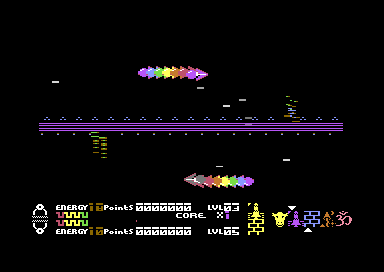
\includegraphics[width=6cm]{planets/entry_images/entry73.png}%
      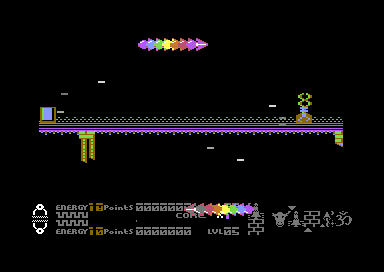
\includegraphics[width=6cm]{planets/entry_images/entry255.png}%
\caption{The planets when we start the materialization sequence, and when we end.}
\end{figure}
